% Options for packages loaded elsewhere
\PassOptionsToPackage{unicode}{hyperref}
\PassOptionsToPackage{hyphens}{url}
%
\documentclass[
  10pt,
  oneside, openany]{book}
\usepackage{amsmath,amssymb}
\usepackage{lmodern}
\usepackage{iftex}
\ifPDFTeX
  \usepackage[T1]{fontenc}
  \usepackage[utf8]{inputenc}
  \usepackage{textcomp} % provide euro and other symbols
\else % if luatex or xetex
  \usepackage{unicode-math}
  \defaultfontfeatures{Scale=MatchLowercase}
  \defaultfontfeatures[\rmfamily]{Ligatures=TeX,Scale=1}
  \setmonofont[]{Lucida Console}
\fi
% Use upquote if available, for straight quotes in verbatim environments
\IfFileExists{upquote.sty}{\usepackage{upquote}}{}
\IfFileExists{microtype.sty}{% use microtype if available
  \usepackage[]{microtype}
  \UseMicrotypeSet[protrusion]{basicmath} % disable protrusion for tt fonts
}{}
\makeatletter
\@ifundefined{KOMAClassName}{% if non-KOMA class
  \IfFileExists{parskip.sty}{%
    \usepackage{parskip}
  }{% else
    \setlength{\parindent}{0pt}
    \setlength{\parskip}{6pt plus 2pt minus 1pt}}
}{% if KOMA class
  \KOMAoptions{parskip=half}}
\makeatother
\usepackage{xcolor}
\usepackage{color}
\usepackage{fancyvrb}
\newcommand{\VerbBar}{|}
\newcommand{\VERB}{\Verb[commandchars=\\\{\}]}
\DefineVerbatimEnvironment{Highlighting}{Verbatim}{commandchars=\\\{\}}
% Add ',fontsize=\small' for more characters per line
\usepackage{framed}
\definecolor{shadecolor}{RGB}{248,248,248}
\newenvironment{Shaded}{\begin{snugshade}}{\end{snugshade}}
\newcommand{\AlertTok}[1]{\textcolor[rgb]{0.94,0.16,0.16}{#1}}
\newcommand{\AnnotationTok}[1]{\textcolor[rgb]{0.56,0.35,0.01}{\textbf{\textit{#1}}}}
\newcommand{\AttributeTok}[1]{\textcolor[rgb]{0.77,0.63,0.00}{#1}}
\newcommand{\BaseNTok}[1]{\textcolor[rgb]{0.00,0.00,0.81}{#1}}
\newcommand{\BuiltInTok}[1]{#1}
\newcommand{\CharTok}[1]{\textcolor[rgb]{0.31,0.60,0.02}{#1}}
\newcommand{\CommentTok}[1]{\textcolor[rgb]{0.56,0.35,0.01}{\textit{#1}}}
\newcommand{\CommentVarTok}[1]{\textcolor[rgb]{0.56,0.35,0.01}{\textbf{\textit{#1}}}}
\newcommand{\ConstantTok}[1]{\textcolor[rgb]{0.00,0.00,0.00}{#1}}
\newcommand{\ControlFlowTok}[1]{\textcolor[rgb]{0.13,0.29,0.53}{\textbf{#1}}}
\newcommand{\DataTypeTok}[1]{\textcolor[rgb]{0.13,0.29,0.53}{#1}}
\newcommand{\DecValTok}[1]{\textcolor[rgb]{0.00,0.00,0.81}{#1}}
\newcommand{\DocumentationTok}[1]{\textcolor[rgb]{0.56,0.35,0.01}{\textbf{\textit{#1}}}}
\newcommand{\ErrorTok}[1]{\textcolor[rgb]{0.64,0.00,0.00}{\textbf{#1}}}
\newcommand{\ExtensionTok}[1]{#1}
\newcommand{\FloatTok}[1]{\textcolor[rgb]{0.00,0.00,0.81}{#1}}
\newcommand{\FunctionTok}[1]{\textcolor[rgb]{0.00,0.00,0.00}{#1}}
\newcommand{\ImportTok}[1]{#1}
\newcommand{\InformationTok}[1]{\textcolor[rgb]{0.56,0.35,0.01}{\textbf{\textit{#1}}}}
\newcommand{\KeywordTok}[1]{\textcolor[rgb]{0.13,0.29,0.53}{\textbf{#1}}}
\newcommand{\NormalTok}[1]{#1}
\newcommand{\OperatorTok}[1]{\textcolor[rgb]{0.81,0.36,0.00}{\textbf{#1}}}
\newcommand{\OtherTok}[1]{\textcolor[rgb]{0.56,0.35,0.01}{#1}}
\newcommand{\PreprocessorTok}[1]{\textcolor[rgb]{0.56,0.35,0.01}{\textit{#1}}}
\newcommand{\RegionMarkerTok}[1]{#1}
\newcommand{\SpecialCharTok}[1]{\textcolor[rgb]{0.00,0.00,0.00}{#1}}
\newcommand{\SpecialStringTok}[1]{\textcolor[rgb]{0.31,0.60,0.02}{#1}}
\newcommand{\StringTok}[1]{\textcolor[rgb]{0.31,0.60,0.02}{#1}}
\newcommand{\VariableTok}[1]{\textcolor[rgb]{0.00,0.00,0.00}{#1}}
\newcommand{\VerbatimStringTok}[1]{\textcolor[rgb]{0.31,0.60,0.02}{#1}}
\newcommand{\WarningTok}[1]{\textcolor[rgb]{0.56,0.35,0.01}{\textbf{\textit{#1}}}}
\usepackage{longtable,booktabs,array}
\usepackage{calc} % for calculating minipage widths
% Correct order of tables after \paragraph or \subparagraph
\usepackage{etoolbox}
\makeatletter
\patchcmd\longtable{\par}{\if@noskipsec\mbox{}\fi\par}{}{}
\makeatother
% Allow footnotes in longtable head/foot
\IfFileExists{footnotehyper.sty}{\usepackage{footnotehyper}}{\usepackage{footnote}}
\makesavenoteenv{longtable}
\usepackage{graphicx}
\makeatletter
\def\maxwidth{\ifdim\Gin@nat@width>\linewidth\linewidth\else\Gin@nat@width\fi}
\def\maxheight{\ifdim\Gin@nat@height>\textheight\textheight\else\Gin@nat@height\fi}
\makeatother
% Scale images if necessary, so that they will not overflow the page
% margins by default, and it is still possible to overwrite the defaults
% using explicit options in \includegraphics[width, height, ...]{}
\setkeys{Gin}{width=\maxwidth,height=\maxheight,keepaspectratio}
% Set default figure placement to htbp
\makeatletter
\def\fps@figure{htbp}
\makeatother
\setlength{\emergencystretch}{3em} % prevent overfull lines
\providecommand{\tightlist}{%
  \setlength{\itemsep}{0pt}\setlength{\parskip}{0pt}}
\setcounter{secnumdepth}{5}
\newlength{\cslhangindent}
\setlength{\cslhangindent}{1.5em}
\newlength{\csllabelwidth}
\setlength{\csllabelwidth}{3em}
\newlength{\cslentryspacingunit} % times entry-spacing
\setlength{\cslentryspacingunit}{\parskip}
\newenvironment{CSLReferences}[2] % #1 hanging-ident, #2 entry spacing
 {% don't indent paragraphs
  \setlength{\parindent}{0pt}
  % turn on hanging indent if param 1 is 1
  \ifodd #1
  \let\oldpar\par
  \def\par{\hangindent=\cslhangindent\oldpar}
  \fi
  % set entry spacing
  \setlength{\parskip}{#2\cslentryspacingunit}
 }%
 {}
\usepackage{calc}
\newcommand{\CSLBlock}[1]{#1\hfill\break}
\newcommand{\CSLLeftMargin}[1]{\parbox[t]{\csllabelwidth}{#1}}
\newcommand{\CSLRightInline}[1]{\parbox[t]{\linewidth - \csllabelwidth}{#1}\break}
\newcommand{\CSLIndent}[1]{\hspace{\cslhangindent}#1}
\let\digamma\undefined

\IfFileExists{lucimatx.sty}{
  % ----- if Lucida availalable------------------
  \usepackage[
    scale=0.875,
    stdmathitalics=true,
    stdmathdigits=true]{lucimatx}
 \linespread{1.02}
}{
  % ------ if Lucida not available --------------
  \usepackage{charter}
  % \usepackage{mathpazo}    % palatino with math
  % \usepackage{mathptmx}    % times with math
  \usepackage{amssymb}
  \linespread{1.03}
}

\usepackage{booktabs}
\usepackage{amsthm}

\usepackage{titlesec}
\titleformat{\chapter}{\bfseries\LARGE}{\thechapter.}{1.5pc}{}{}
\titlespacing{\chapter}{0pt}{0pt}{12pt}
\titleformat{\section}{\bfseries\large}{\thesection.}{1em}{}
\titlespacing{\section}{0pt}{8pt}{3pt}
\titleformat{\subsection}{\bfseries}{}{0em}{}
\titlespacing{\subsection}{0pt}{6pt}{1pt}
\titleformat{\subsubsection}{\slshape}{}{0em}{}
\titlespacing{\subsection}{0pt}{6pt}{1pt}

\usepackage[titles]{tocloft}
\renewcommand{\cftpartfont}{\normalsize\rm\bfseries}
\renewcommand{\cftpartpagefont}{\normalsize\rm\bfseries}
\setlength{\cftbeforechapskip}{2ex}
\setlength{\cftchapnumwidth}{3ex}
\renewcommand{\cftchapfont}{\normalsize\bf}
\renewcommand{\cftchappagefont}{\footnotesize\rm}
\renewcommand{\cftchapaftersnum}{.}
\renewcommand{\cftchapaftersnumb}{\hspace*{8pt}}
\renewcommand{\cftchapleader}{\hspace*{1em}}
\renewcommand{\cftchapafterpnum}{\cftparfillskip}
\renewcommand{\cftpnumalign}{l}
\setlength{\cftbeforesecskip}{0.5ex}
\setlength{\cftsecnumwidth}{5.5ex}
\setlength{\cftsecindent}{5ex}
\renewcommand{\cftsecfont}{\small}
\renewcommand{\cftsecpagefont}{\footnotesize}
\renewcommand{\cftsecaftersnum}{}
\renewcommand{\cftsecaftersnumb}{\hspace*{8pt}}
\renewcommand{\cftsecleader}{\hspace*{1em}}
\renewcommand{\cftsecafterpnum}{\cftparfillskip}
\renewcommand{\cftpnumalign}{l}

\setlength{\paperwidth}{6in}
\setlength{\paperheight}{8in}
\pdfpagewidth=\paperwidth
\pdfpageheight=\paperheight

\setlength{\textwidth}{5in}
\setlength{\textheight}{6.75in}
\setlength{\oddsidemargin}{-0.5in}
\setlength{\evensidemargin}{-0.5in}
\setlength{\topmargin}{-0.75in}
\setlength{\headsep}{18pt}

\renewcommand{\topfraction}{0.9}
\renewcommand{\bottomfraction}{0.8}
\renewcommand{\floatpagefraction}{0.75}
\renewcommand{\textfraction}{0.07}

\setcounter{tocdepth}{0}

\raggedbottom
\sloppy

\let\cleardoublepage\clearpage
\usepackage{booktabs}
\usepackage{longtable}
\usepackage{array}
\usepackage{multirow}
\usepackage{wrapfig}
\usepackage{float}
\usepackage{colortbl}
\usepackage{pdflscape}
\usepackage{tabu}
\usepackage{threeparttable}
\usepackage{threeparttablex}
\usepackage[normalem]{ulem}
\usepackage{makecell}
\usepackage{xcolor}
\ifLuaTeX
  \usepackage{selnolig}  % disable illegal ligatures
\fi
\IfFileExists{bookmark.sty}{\usepackage{bookmark}}{\usepackage{hyperref}}
\IfFileExists{xurl.sty}{\usepackage{xurl}}{} % add URL line breaks if available
\urlstyle{same} % disable monospaced font for URLs
\hypersetup{
  pdftitle={Stan User's Guide},
  pdfauthor={Stan Development Team},
  hidelinks,
  pdfcreator={LaTeX via pandoc}}

\title{Stan User's Guide}
\usepackage{etoolbox}
\makeatletter
\providecommand{\subtitle}[1]{% add subtitle to \maketitle
  \apptocmd{\@title}{\par {\large #1 \par}}{}{}
}
\makeatother
\subtitle{Version 2.32}
\author{Stan Development Team}
\date{}

\begin{document}
\maketitle

{
\setcounter{tocdepth}{1}
\tableofcontents
}
\hypertarget{overview}{%
\chapter*{Overview}\label{overview}}
\addcontentsline{toc}{chapter}{Overview}

\hypertarget{about-this-users-guide}{%
\subsubsection*{About this user's guide}\label{about-this-users-guide}}
\addcontentsline{toc}{subsubsection}{About this user's guide}

This is the official user's guide for Stan. It provides example
models and programming techniques for coding statistical models in Stan.

\begin{itemize}
\item
  Part 1 gives Stan code and discussions for several important classes
  of models.
\item
  Part 2 discusses various general Stan programming techniques that are
  not tied to any particular model.
\item
  Part 3 introduces algorithms for calibration and model checking that
  require multiple runs of Stan.
\item
  The appendices provide an introduction to the stanc3 compiler used in the
  various interfaces to Stan, a style guide, and advice for users of BUGS and
  JAGS.
\end{itemize}

In addition to this user's guide, there are two reference manuals for
the Stan language and algorithms. The \href{https://mc-stan.org/docs/reference-manual/index.html}{\emph{Stan Reference Manual}}
specifies the Stan programming language and inference algorithms. The
\href{https://mc-stan.org/docs/functions-reference/index.html}{\emph{Stan Functions Reference}}
specifies the functions built into the Stan programming language.

There is also a separate installation and getting started guide for
each of the Stan \href{https://mc-stan.org/users/interfaces/}{interfaces} (R, Python,
Julia, Stata, MATLAB, Mathematica, and command line).

We recommend working through this guide using the textbooks \emph{Bayesian
Data Analysis} and \emph{Statistical Rethinking: A Bayesian Course with
Examples in R and Stan} as references on the concepts, and using the
\href{https://mc-stan.org/docs/reference-manual/index.html}{\emph{Stan Reference Manual}}
when necessary to clarify programming issues.

\hypertarget{web-resources}{%
\subsubsection*{Web resources}\label{web-resources}}
\addcontentsline{toc}{subsubsection}{Web resources}

Stan is an open-source software project, resources for which are
hosted on various web sites:

\begin{itemize}
\item
  The \href{https://mc-stan.org/}{Stan Web Site} organizes all of the resources
  for the Stan project for users and developers. It contains links to
  the official Stan releases, source code, installation instructions,
  and full documentation, including the latest version of this manual,
  the user's guide and the getting started guide for each interface,
  tutorials, case studies, and reference materials for developers.
\item
  The \href{https://discourse.mc-stan.org}{Stan Forums} provide structured
  message boards for questions, discussion, and announcements related to
  Stan for both users and developers.
\item
  The \href{https://github.com/stan-dev}{Stan GitHub Organization} hosts all
  of Stan's code, documentation, wikis, and web site, as well as the
  issue trackers for bug reports and feature requests and interactive
  code review for pull requests.
\end{itemize}

\hypertarget{acknowledgements}{%
\subsubsection*{Acknowledgements}\label{acknowledgements}}
\addcontentsline{toc}{subsubsection}{Acknowledgements}

The Stan project could not exist without developers, users, and
funding. Stan is a highly collaborative project. The individual
contributions of the Stan developers to code is tracked through GitHub
and to the design conversation in the Wikis and forums.

Users have made extensive contributions to documentation in the way
of case studies, tutorials and even books. They have also reported
numerous bugs in both the code and documentation.

Stan has been funded through grants for Stan and its developers,
through in-kind donations in the form of companies contributing
developer time to Stan and individuals contributing their own time to
Stan, and through donations to the open-source scientific software
non-profit NumFOCUS. For details of direct funding for the project,
see the web site and project pages of the Stan developers.

\hypertarget{copyright-trademark-and-licensing}{%
\subsubsection*{Copyright, trademark, and licensing}\label{copyright-trademark-and-licensing}}
\addcontentsline{toc}{subsubsection}{Copyright, trademark, and licensing}

This book is copyright 2011--2022, Stan Development Team and their
assignees. The text content is distributed under the \href{https://creativecommons.org/licenses/by-nd/4.0/legalcode}{CC BY-ND 4.0
license}.
The user's guide R and Stan programs are distributed under the \href{https://opensource.org/licenses/BSD-3-Clause}{BSD
3-clause license}.

The Stan name and logo are registered trademarks of NumFOCUS. Use of
the Stan name and logo are governed by the \href{https://mc-stan.org/about/logo/}{Stan logo usage
guidelines}.

\hypertarget{example-models.part}{%
\chapter*{Part 1. Example Models}\label{example-models.part}}
\addcontentsline{toc}{chapter}{Part 1. Example Models}

In this part of the book, we survey a range of example models,
with the goal of illustrating how to code them efficiently in Stan.

\hypertarget{regression-models}{%
\chapter{Regression Models}\label{regression-models}}

Stan supports regression models from simple linear regressions to
multilevel generalized linear models.

\hypertarget{linear-regression}{%
\section{Linear regression}\label{linear-regression}}

The simplest linear regression model is the following, with a single
predictor and a slope and intercept coefficient, and normally
distributed noise. This model can be written using standard
regression notation as
\[
y_n = \alpha + \beta x_n + \epsilon_n
\quad\text{where}\quad
\epsilon_n \sim \operatorname{normal}(0,\sigma).
\]

This is equivalent to the following sampling involving the
residual,
\[
y_n - (\alpha + \beta X_n) \sim \operatorname{normal}(0,\sigma),
\]
and reducing still further, to
\[
y_n \sim \operatorname{normal}(\alpha + \beta X_n, \, \sigma).
\]

This latter form of the model is coded in Stan as follows.

\begin{Shaded}
\begin{Highlighting}[]
\KeywordTok{data}\NormalTok{ \{}
  \DataTypeTok{int}\NormalTok{\textless{}}\KeywordTok{lower}\NormalTok{=}\DecValTok{0}\NormalTok{\textgreater{} N;}
  \DataTypeTok{vector}\NormalTok{[N] x;}
  \DataTypeTok{vector}\NormalTok{[N] y;}
\NormalTok{\}}
\KeywordTok{parameters}\NormalTok{ \{}
  \DataTypeTok{real}\NormalTok{ alpha;}
  \DataTypeTok{real}\NormalTok{ beta;}
  \DataTypeTok{real}\NormalTok{\textless{}}\KeywordTok{lower}\NormalTok{=}\DecValTok{0}\NormalTok{\textgreater{} sigma;}
\NormalTok{\}}
\KeywordTok{model}\NormalTok{ \{}
\NormalTok{  y \textasciitilde{} normal(alpha + beta * x, sigma);}
\NormalTok{\}}
\end{Highlighting}
\end{Shaded}

There are \texttt{N} observations and for each observation, \(n \in N\), we have predictor
\texttt{x{[}n{]}} and outcome \texttt{y{[}n{]}}. The intercept and slope parameters are
\texttt{alpha} and \texttt{beta}. The model assumes a normally
distributed noise term with scale \texttt{sigma}. This model has
improper priors for the two regression coefficients.

\hypertarget{vectorization.section}{%
\subsection*{Matrix notation and vectorization}\label{vectorization.section}}
\addcontentsline{toc}{subsection}{Matrix notation and vectorization}

The sampling statement in the previous model is vectorized, with

\begin{Shaded}
\begin{Highlighting}[]
\NormalTok{y \textasciitilde{} normal(alpha + beta * x, sigma);}
\end{Highlighting}
\end{Shaded}

providing the same model as the unvectorized version,

\begin{Shaded}
\begin{Highlighting}[]
\ControlFlowTok{for}\NormalTok{ (n }\ControlFlowTok{in} \DecValTok{1}\NormalTok{:N) \{}
\NormalTok{  y[n] \textasciitilde{} normal(alpha + beta * x[n], sigma);}
\NormalTok{\}}
\end{Highlighting}
\end{Shaded}

In addition to being more concise, the vectorized form is much faster.\footnote{Unlike in Python and R, which are interpreted, Stan is translated to C++ and compiled, so loops and assignment statements are fast. Vectorized code is faster in Stan because (a) the expression tree used to compute derivatives can be simplified, leading to fewer virtual function calls, and (b) computations that would be repeated in the looping version, such as \texttt{log(sigma)} in the above model, will be computed once and reused.}

In general, Stan allows the arguments to distributions such as
\texttt{normal} to be vectors. If any of the other arguments are vectors or
arrays, they have to be the same size. If any of the other arguments
is a scalar, it is reused for each vector entry. See \protect\hyperlink{vectorization.section}{the
vectorization section} for more information on
vectorization of probability functions.

The other reason this works is that Stan's arithmetic operators are
overloaded to perform matrix arithmetic on matrices. In this case,
because \texttt{x} is of type \texttt{vector} and \texttt{beta} of type
\texttt{real}, the expression \texttt{beta\ *\ x} is of type \texttt{vector}.
Because Stan supports vectorization, a regression model with more than
one predictor can be written directly using matrix notation.

\begin{Shaded}
\begin{Highlighting}[]
\KeywordTok{data}\NormalTok{ \{}
  \DataTypeTok{int}\NormalTok{\textless{}}\KeywordTok{lower}\NormalTok{=}\DecValTok{0}\NormalTok{\textgreater{} N;   }\CommentTok{// number of data items}
  \DataTypeTok{int}\NormalTok{\textless{}}\KeywordTok{lower}\NormalTok{=}\DecValTok{0}\NormalTok{\textgreater{} K;   }\CommentTok{// number of predictors}
  \DataTypeTok{matrix}\NormalTok{[N, K] x;   }\CommentTok{// predictor matrix}
  \DataTypeTok{vector}\NormalTok{[N] y;      }\CommentTok{// outcome vector}
\NormalTok{\}}
\KeywordTok{parameters}\NormalTok{ \{}
  \DataTypeTok{real}\NormalTok{ alpha;           }\CommentTok{// intercept}
  \DataTypeTok{vector}\NormalTok{[K] beta;       }\CommentTok{// coefficients for predictors}
  \DataTypeTok{real}\NormalTok{\textless{}}\KeywordTok{lower}\NormalTok{=}\DecValTok{0}\NormalTok{\textgreater{} sigma;  }\CommentTok{// error scale}
\NormalTok{\}}
\KeywordTok{model}\NormalTok{ \{}
\NormalTok{  y \textasciitilde{} normal(x * beta + alpha, sigma);  }\CommentTok{// likelihood}
\NormalTok{\}}
\end{Highlighting}
\end{Shaded}

The constraint \texttt{lower=0} in the declaration of \texttt{sigma}
constrains the value to be greater than or equal to 0. With no prior
in the model block, the effect is an improper prior on non-negative
real numbers. Although a more informative prior may be added, improper
priors are acceptable as long as they lead to proper posteriors.

In the model above, \texttt{x} is an \(N \times K\) matrix of predictors
and \texttt{beta} a \(K\)-vector of coefficients, so \texttt{x\ *\ beta} is an
\(N\)-vector of predictions, one for each of the \(N\) data items. These
predictions line up with the outcomes in the \(N\)-vector \texttt{y}, so
the entire model may be written using matrix arithmetic as shown. It
would be possible to include a column of ones in the data matrix \texttt{x} to
remove the \texttt{alpha} parameter.

The sampling statement in the model above is just a more efficient,
vector-based approach to coding the model with a loop, as in the
following statistically equivalent model.

\begin{Shaded}
\begin{Highlighting}[]
\KeywordTok{model}\NormalTok{ \{}
  \ControlFlowTok{for}\NormalTok{ (n }\ControlFlowTok{in} \DecValTok{1}\NormalTok{:N) \{}
\NormalTok{    y[n] \textasciitilde{} normal(x[n] * beta, sigma);}
\NormalTok{  \}}
\NormalTok{\}}
\end{Highlighting}
\end{Shaded}

With Stan's matrix indexing scheme, \texttt{x{[}n{]}} picks out row \texttt{n}
of the matrix \texttt{x}; because \texttt{beta} is a column vector,
the product \texttt{x{[}n{]}\ *\ beta} is a scalar of type \texttt{real}.

\hypertarget{intercepts-as-inputs}{%
\subsubsection*{Intercepts as inputs}\label{intercepts-as-inputs}}
\addcontentsline{toc}{subsubsection}{Intercepts as inputs}

In the model formulation

\begin{Shaded}
\begin{Highlighting}[]
\NormalTok{y \textasciitilde{} normal(x * beta, sigma);}
\end{Highlighting}
\end{Shaded}

there is no longer an intercept coefficient \texttt{alpha}. Instead, we
have assumed that the first column of the input matrix \texttt{x} is a
column of 1 values. This way, \texttt{beta{[}1{]}} plays the role of the
intercept. If the intercept gets a different prior than the slope
terms, then it would be clearer to break it out. It is also slightly
more efficient in its explicit form with the intercept variable
singled out because there's one fewer multiplications; it should not
make that much of a difference to speed, though, so the choice should
be based on clarity.

\hypertarget{QR-reparameterization.section}{%
\section{The QR reparameterization}\label{QR-reparameterization.section}}

In the previous example, the linear predictor can be written as \(\eta = x \beta\), where \(\eta\) is a \(N\)-vector of predictions, \(x\) is a \(N \times K\) matrix, and \(\beta\) is a \(K\)-vector of coefficients.
Presuming \(N \geq K\), we can exploit the fact that any design matrix
\(x\) can be decomposed using the thin QR decomposition into an
orthogonal matrix \(Q\) and an upper-triangular matrix \(R\), i.e.~\(x = Q R\).

The functions \texttt{qr\_thin\_Q} and \texttt{qr\_thin\_R} implement the thin QR decomposition,
which is to be preferred to the fat QR decomposition that would be obtained
by using \texttt{qr\_Q} and \texttt{qr\_R}, as the latter would more easily run out of memory
(see the Stan Functions Reference for more information on the \texttt{qr\_thin\_Q}
and \texttt{qr\_thin\_R} functions). In practice, it is best to write \(x = Q^\ast R^\ast\) where \(Q^\ast = Q * \sqrt{n - 1}\) and \(R^\ast = \frac{1}{\sqrt{n - 1}} R\). Thus, we can equivalently write \(\eta = x \beta = Q R \beta = Q^\ast R^\ast \beta\). If we let \(\theta = R^\ast \beta\), then we have \(\eta = Q^\ast \theta\) and \(\beta = R^{\ast^{-1}} \theta\). In that case, the previous Stan program becomes

\begin{Shaded}
\begin{Highlighting}[]
\KeywordTok{data}\NormalTok{ \{}
  \DataTypeTok{int}\NormalTok{\textless{}}\KeywordTok{lower}\NormalTok{=}\DecValTok{0}\NormalTok{\textgreater{} N;   }\CommentTok{// number of data items}
  \DataTypeTok{int}\NormalTok{\textless{}}\KeywordTok{lower}\NormalTok{=}\DecValTok{0}\NormalTok{\textgreater{} K;   }\CommentTok{// number of predictors}
  \DataTypeTok{matrix}\NormalTok{[N, K] x;   }\CommentTok{// predictor matrix}
  \DataTypeTok{vector}\NormalTok{[N] y;      }\CommentTok{// outcome vector}
\NormalTok{\}}
\KeywordTok{transformed data}\NormalTok{ \{}
  \DataTypeTok{matrix}\NormalTok{[N, K] Q\_ast;}
  \DataTypeTok{matrix}\NormalTok{[K, K] R\_ast;}
  \DataTypeTok{matrix}\NormalTok{[K, K] R\_ast\_inverse;}
  \CommentTok{// thin and scale the QR decomposition}
\NormalTok{  Q\_ast = qr\_thin\_Q(x) * sqrt(N {-} }\DecValTok{1}\NormalTok{);}
\NormalTok{  R\_ast = qr\_thin\_R(x) / sqrt(N {-} }\DecValTok{1}\NormalTok{);}
\NormalTok{  R\_ast\_inverse = inverse(R\_ast);}
\NormalTok{\}}
\KeywordTok{parameters}\NormalTok{ \{}
  \DataTypeTok{real}\NormalTok{ alpha;           }\CommentTok{// intercept}
  \DataTypeTok{vector}\NormalTok{[K] theta;      }\CommentTok{// coefficients on Q\_ast}
  \DataTypeTok{real}\NormalTok{\textless{}}\KeywordTok{lower}\NormalTok{=}\DecValTok{0}\NormalTok{\textgreater{} sigma;  }\CommentTok{// error scale}
\NormalTok{\}}
\KeywordTok{model}\NormalTok{ \{}
\NormalTok{  y \textasciitilde{} normal(Q\_ast * theta + alpha, sigma);  }\CommentTok{// likelihood}
\NormalTok{\}}
\KeywordTok{generated quantities}\NormalTok{ \{}
  \DataTypeTok{vector}\NormalTok{[K] beta;}
\NormalTok{  beta = R\_ast\_inverse * theta; }\CommentTok{// coefficients on x}
\NormalTok{\}}
\end{Highlighting}
\end{Shaded}

Since this Stan program generates equivalent predictions for \(y\) and
the same posterior distribution for \(\alpha\), \(\beta\), and \(\sigma\) as
the previous Stan program, many wonder why the version with this QR
reparameterization performs so much better in practice, often both in
terms of wall time and in terms of effective sample size. The
reasoning is threefold:

\begin{enumerate}
\def\labelenumi{\arabic{enumi}.}
\item
  The columns of \(Q^\ast\) are orthogonal whereas the columns of
  \(x\) generally are not. Thus, it is easier for a Markov Chain to move
  around in \(\theta\)-space than in \(\beta\)-space.
\item
  The columns of \(Q^\ast\) have the same scale whereas the columns
  of \(x\) generally do not. Thus, a Hamiltonian Monte Carlo algorithm
  can move around the parameter space with a smaller number of larger
  steps
\item
  Since the covariance matrix for the columns of \(Q^\ast\) is an
  identity matrix, \(\theta\) typically has a reasonable scale if the
  units of \(y\) are also reasonable. This also helps HMC move
  efficiently without compromising numerical accuracy.
\end{enumerate}

Consequently, this QR reparameterization is recommended for linear and
generalized linear models in Stan whenever \(K > 1\) and you do not have
an informative prior on the location of \(\beta\). It can also be
worthwhile to subtract the mean from each column of \(x\) before
obtaining the QR decomposition, which does not affect the posterior
distribution of \(\theta\) or \(\beta\) but does affect \(\alpha\) and
allows you to interpret \(\alpha\) as the expectation of \(y\) in a linear
model.

\hypertarget{regression-priors.section}{%
\section{Priors for coefficients and scales}\label{regression-priors.section}}

See our \href{https://github.com/stan-dev/stan/wiki/Prior-Choice-Recommendations}{general discussion of priors}
for tips on priors for parameters in regression models.

Later sections discuss \protect\hyperlink{hierarchical-priors.section}{univariate
hierarchical priors} and \protect\hyperlink{multivariate-hierarchical-priors.section}{multivariate
hierarchical priors}, as well
as \protect\hyperlink{priors-for-identification.section}{priors used to identify models}.

However, as described in \protect\hyperlink{QR-reparameterization.section}{QR-reparameterization
section}, if you do not have an
informative prior on the \emph{location} of the regression coefficients,
then you are better off reparameterizing your model so that the
regression coefficients are a generated quantity. In that case, it
usually does not matter much what prior is used on on the
reparameterized regression coefficients and almost any weakly
informative prior that scales with the outcome will do.

\hypertarget{robust-noise-models}{%
\section{Robust noise models}\label{robust-noise-models}}

The standard approach to linear regression is to model the noise
term \(\epsilon\) as having a normal distribution. From Stan's
perspective, there is nothing special about normally distributed
noise. For instance, robust regression can be accommodated by giving
the noise term a Student-\(t\) distribution. To code this in Stan, the
sampling distribution is changed to the following.

\begin{Shaded}
\begin{Highlighting}[]
\KeywordTok{data}\NormalTok{ \{}
  \CommentTok{// ...}
  \DataTypeTok{real}\NormalTok{\textless{}}\KeywordTok{lower}\NormalTok{=}\DecValTok{0}\NormalTok{\textgreater{} nu;}
\NormalTok{\}}
\CommentTok{// ...}
\KeywordTok{model}\NormalTok{ \{}
\NormalTok{  y \textasciitilde{} student\_t(nu, alpha + beta * x, sigma);}
\NormalTok{\}}
\end{Highlighting}
\end{Shaded}

The degrees of freedom constant \texttt{nu} is specified as data.

\hypertarget{logistic-probit-regression.section}{%
\section{Logistic and probit regression}\label{logistic-probit-regression.section}}

For binary outcomes, either of the closely related logistic or probit
regression models may be used. These generalized linear models vary
only in the link function they use to map linear predictions in
\((-\infty,\infty)\) to probability values in \((0,1)\). Their respective
link functions, the logistic function and the standard normal cumulative distribution
function, are both sigmoid functions (i.e., they are both \emph{S}-shaped).

A logistic regression model with one predictor and an intercept is coded as
follows.

\begin{Shaded}
\begin{Highlighting}[]
\KeywordTok{data}\NormalTok{ \{}
  \DataTypeTok{int}\NormalTok{\textless{}}\KeywordTok{lower}\NormalTok{=}\DecValTok{0}\NormalTok{\textgreater{} N;}
  \DataTypeTok{vector}\NormalTok{[N] x;}
  \DataTypeTok{array}\NormalTok{[N] }\DataTypeTok{int}\NormalTok{\textless{}}\KeywordTok{lower}\NormalTok{=}\DecValTok{0}\NormalTok{, }\KeywordTok{upper}\NormalTok{=}\DecValTok{1}\NormalTok{\textgreater{} y;}
\NormalTok{\}}
\KeywordTok{parameters}\NormalTok{ \{}
  \DataTypeTok{real}\NormalTok{ alpha;}
  \DataTypeTok{real}\NormalTok{ beta;}
\NormalTok{\}}
\KeywordTok{model}\NormalTok{ \{}
\NormalTok{  y \textasciitilde{} bernoulli\_logit(alpha + beta * x);}
\NormalTok{\}}
\end{Highlighting}
\end{Shaded}

The noise parameter is built into the Bernoulli formulation here
rather than specified directly.

Logistic regression is a kind of generalized linear model with binary
outcomes and the log odds (logit) link function, defined by
\[
\operatorname{logit}(v) = \log \left( \frac{v}{1-v} \right).
\]

The inverse of the link function appears in the model:
\[
\operatorname{logit}^{-1}(u) = \texttt{inv}\mathtt{\_}\texttt{logit}(u) = \frac{1}{1 + \exp(-u)}.
\]

The model formulation above uses the logit-parameterized version of
the Bernoulli distribution, which is defined by
\[
\texttt{bernoulli}\mathtt{\_}\texttt{logit}\left(y \mid \alpha \right)
=
\texttt{bernoulli}\left(y \mid \operatorname{logit}^{-1}(\alpha)\right).
\]

The formulation is also vectorized in the sense that \texttt{alpha} and
\texttt{beta} are scalars and \texttt{x} is a vector, so that \texttt{alpha\ \ \ +\ beta\ *\ x} is a vector. The vectorized formulation is equivalent
to the less efficient version

\begin{Shaded}
\begin{Highlighting}[]
\ControlFlowTok{for}\NormalTok{ (n }\ControlFlowTok{in} \DecValTok{1}\NormalTok{:N) \{}
\NormalTok{  y[n] \textasciitilde{} bernoulli\_logit(alpha + beta * x[n]);}
\NormalTok{\}}
\end{Highlighting}
\end{Shaded}

Expanding out the Bernoulli logit, the model is equivalent to the more
explicit, but less efficient and less arithmetically stable

\begin{Shaded}
\begin{Highlighting}[]
\ControlFlowTok{for}\NormalTok{ (n }\ControlFlowTok{in} \DecValTok{1}\NormalTok{:N) \{}
\NormalTok{  y[n] \textasciitilde{} bernoulli(inv\_logit(alpha + beta * x[n]));}
\NormalTok{\}}
\end{Highlighting}
\end{Shaded}

Other link functions may be used in the same way. For example, probit
regression uses the cumulative normal distribution function, which is
typically written as

\[
\Phi(x) = \int_{-\infty}^x \textsf{normal}\left(y \mid 0,1 \right) \,\textrm{d}y.
\]

The cumulative standard normal distribution function \(\Phi\) is implemented
in Stan as the function \texttt{Phi}. The probit regression model
may be coded in Stan by replacing the logistic model's sampling
statement with the following.

\begin{Shaded}
\begin{Highlighting}[]
\NormalTok{y[n] \textasciitilde{} bernoulli(Phi(alpha + beta * x[n]));}
\end{Highlighting}
\end{Shaded}

A fast approximation to the cumulative standard normal distribution
function \(\Phi\) is implemented in Stan as the function
\texttt{Phi\_approx}.\footnote{The \texttt{Phi\_approx} function is a rescaled version of the inverse logit function, so while the scale is roughly the same \(\Phi\), the tails do not match.}
The approximate probit regression model may
be coded with the following.

\begin{Shaded}
\begin{Highlighting}[]
\NormalTok{y[n] \textasciitilde{} bernoulli(Phi\_approx(alpha + beta * x[n]));}
\end{Highlighting}
\end{Shaded}

\hypertarget{multi-logit.section}{%
\section{Multi-logit regression}\label{multi-logit.section}}

Multiple outcome forms of logistic regression can be coded directly in
Stan. For instance, suppose there are \(K\) possible outcomes for each
output variable \(y_n\). Also suppose that there is a \(D\)-dimensional
vector \(x_n\) of predictors for \(y_n\). The multi-logit model with
\(\textsf{normal}(0,5)\) priors on the coefficients is coded as follows.

\begin{Shaded}
\begin{Highlighting}[]
\KeywordTok{data}\NormalTok{ \{}
  \DataTypeTok{int}\NormalTok{ K;}
  \DataTypeTok{int}\NormalTok{ N;}
  \DataTypeTok{int}\NormalTok{ D;}
  \DataTypeTok{array}\NormalTok{[N] }\DataTypeTok{int}\NormalTok{ y;}
  \DataTypeTok{matrix}\NormalTok{[N, D] x;}
\NormalTok{\}}
\KeywordTok{parameters}\NormalTok{ \{}
  \DataTypeTok{matrix}\NormalTok{[D, K] beta;}
\NormalTok{\}}
\KeywordTok{model}\NormalTok{ \{}
  \DataTypeTok{matrix}\NormalTok{[N, K] x\_beta = x * beta;}

\NormalTok{  to\_vector(beta) \textasciitilde{} normal(}\DecValTok{0}\NormalTok{, }\DecValTok{5}\NormalTok{);}

  \ControlFlowTok{for}\NormalTok{ (n }\ControlFlowTok{in} \DecValTok{1}\NormalTok{:N) \{}
\NormalTok{    y[n] \textasciitilde{} categorical\_logit(x\_beta[n]\textquotesingle{});}

\NormalTok{  \}}
\NormalTok{\}}
\end{Highlighting}
\end{Shaded}

where \texttt{x\_beta{[}n{]}\textquotesingle{}} is the transpose of \texttt{x\_beta{[}n{]}}. The prior on \texttt{beta} is coded in vectorized form.
As of Stan 2.18, the categorical-logit distribution is not vectorized
for parameter arguments, so the loop is required. The matrix multiplication
is pulled out to define a local variable for all of the predictors for
efficiency. Like the Bernoulli-logit, the categorical-logit
distribution applies softmax internally to convert an arbitrary vector
to a simplex,
\[
\texttt{categorical}\mathtt{\_}\texttt{logit}\left(y \mid \alpha\right)
=
\texttt{categorical}\left(y \mid \texttt{softmax}(\alpha)\right),
\]
where
\[
\texttt{softmax}(u) = \exp(u) / \operatorname{sum}\left(\exp(u)\right).
\]

The categorical distribution with log-odds (logit) scaled parameters
used above is equivalent to writing

\begin{Shaded}
\begin{Highlighting}[]
\NormalTok{y[n] \textasciitilde{} categorical(softmax(x[n] * beta));}
\end{Highlighting}
\end{Shaded}

\hypertarget{constraints-on-data-declarations}{%
\subsubsection*{Constraints on data declarations}\label{constraints-on-data-declarations}}
\addcontentsline{toc}{subsubsection}{Constraints on data declarations}

The data block in the above model is defined without constraints on
sizes \texttt{K}, \texttt{N}, and \texttt{D} or on the outcome array
\texttt{y}. Constraints on data declarations provide error checking at
the point data are read (or transformed data are defined), which is
before sampling begins. Constraints on data declarations also make
the model author's intentions more explicit, which can help with
readability. The above model's declarations could be tightened to

\begin{Shaded}
\begin{Highlighting}[]
\DataTypeTok{int}\NormalTok{\textless{}}\KeywordTok{lower}\NormalTok{=}\DecValTok{2}\NormalTok{\textgreater{} K;}
\DataTypeTok{int}\NormalTok{\textless{}}\KeywordTok{lower}\NormalTok{=}\DecValTok{0}\NormalTok{\textgreater{} N;}
\DataTypeTok{int}\NormalTok{\textless{}}\KeywordTok{lower}\NormalTok{=}\DecValTok{1}\NormalTok{\textgreater{} D;}
\DataTypeTok{array}\NormalTok{[N] }\DataTypeTok{int}\NormalTok{\textless{}}\KeywordTok{lower}\NormalTok{=}\DecValTok{1}\NormalTok{, }\KeywordTok{upper}\NormalTok{=K\textgreater{} y;}
\end{Highlighting}
\end{Shaded}

These constraints arise because the number of categories, \texttt{K},
must be at least two in order for a categorical model to be useful.
The number of data items, \texttt{N}, can be zero, but not negative;
unlike R, Stan's for-loops always move forward, so that a loop extent
of \texttt{1:N} when \texttt{N} is equal to zero ensures the loop's body
will not be executed. The number of predictors, \texttt{D}, must be at
least one in order for \texttt{beta\ *\ x{[}n{]}} to produce an
appropriate argument for \texttt{softmax()}. The categorical outcomes
\texttt{y{[}n{]}} must be between \texttt{1} and \texttt{K} in order for the
discrete sampling to be well defined.

Constraints on data declarations are optional. Constraints on
parameters declared in the \texttt{parameters} block, on the other hand,
are \emph{not} optional---they are required to ensure support for all
parameter values satisfying their constraints. Constraints on
transformed data, transformed parameters, and generated quantities are
also optional.

\hypertarget{identifiability}{%
\subsection*{Identifiability}\label{identifiability}}
\addcontentsline{toc}{subsection}{Identifiability}

Because softmax is invariant under adding a constant to each component
of its input, the model is typically only identified if there is a
suitable prior on the coefficients.

An alternative is to use \((K-1)\)-vectors by fixing one of them to be
zero. The \protect\hyperlink{partially-known-parameters.section}{partially known parameters
section} discusses how to mix
constants and parameters in a vector. In the multi-logit case, the
parameter block would be redefined to use \((K - 1)\)-vectors

\begin{Shaded}
\begin{Highlighting}[]
\KeywordTok{parameters}\NormalTok{ \{}
  \DataTypeTok{matrix}\NormalTok{[D, K {-} }\DecValTok{1}\NormalTok{] beta\_raw;}
\NormalTok{\}}
\end{Highlighting}
\end{Shaded}

and then these are transformed to parameters to use in the model.
First, a transformed data block is added before the parameters block
to define a vector of zero values,

\begin{Shaded}
\begin{Highlighting}[]
\KeywordTok{transformed data}\NormalTok{ \{}
  \DataTypeTok{vector}\NormalTok{[D] zeros = rep\_vector(}\DecValTok{0}\NormalTok{, D);}
\NormalTok{\}}
\end{Highlighting}
\end{Shaded}

which can then be appended to \texttt{beta\_raw} to produce the
coefficient matrix \texttt{beta},

\begin{Shaded}
\begin{Highlighting}[]
\KeywordTok{transformed parameters}\NormalTok{ \{}
  \DataTypeTok{matrix}\NormalTok{[D, K] beta = append\_col(beta\_raw, zeros);}
\NormalTok{\}}
\end{Highlighting}
\end{Shaded}

The \texttt{rep\_vector(0,\ D)} call creates a column vector of size \texttt{D} with
all entries set to zero. The derived matrix \texttt{beta} is then defined to
be the result of appending the vector \texttt{zeros} as a new column at the
end of \texttt{beta\_raw}; the vector \texttt{zeros} is defined as transformed
data so that it doesn't need to be constructed from scratch each time
it is used.

This is not the same model as using \(K\)-vectors as parameters,
because now the prior only applies to \((K-1)\)-vectors. In practice,
this will cause the maximum likelihood solutions to be different and
also the posteriors to be slightly different when taking priors
centered around zero, as is typical for regression coefficients.

\hypertarget{parameterizing-centered-vectors}{%
\section{Parameterizing centered vectors}\label{parameterizing-centered-vectors}}

It is often convenient to define a parameter vector \(\beta\) that is
centered in the sense of satisfying the sum-to-zero constraint,
\[
\sum_{k=1}^K \beta_k = 0.
\]

Such a parameter vector may be used to identify a multi-logit
regression parameter vector (see the \protect\hyperlink{multi-logit.section}{multi-logit
section} for details), or may be used for
ability or difficulty parameters (but not both) in an IRT model (see
the \protect\hyperlink{item-response-models.section}{item-response model section} for
details).

\hypertarget{k-1-degrees-of-freedom}{%
\subsection*{\texorpdfstring{\(K-1\) degrees of freedom}{K-1 degrees of freedom}}\label{k-1-degrees-of-freedom}}
\addcontentsline{toc}{subsection}{\(K-1\) degrees of freedom}

There is more than one way to enforce a sum-to-zero constraint on a
parameter vector, the most efficient of which is to define the \(K\)-th
element as the negation of the sum of the elements \(1\) through \(K-1\).

\begin{Shaded}
\begin{Highlighting}[]
\KeywordTok{parameters}\NormalTok{ \{}
  \DataTypeTok{vector}\NormalTok{[K {-} }\DecValTok{1}\NormalTok{] beta\_raw;}
  \CommentTok{// ...}
\NormalTok{\}}
\KeywordTok{transformed parameters}\NormalTok{ \{}
  \DataTypeTok{vector}\NormalTok{[K] beta = append\_row(beta\_raw, {-}sum(beta\_raw));}
  \CommentTok{// ...}
\NormalTok{\}}
\end{Highlighting}
\end{Shaded}

Placing a prior on \texttt{beta\_raw} in this parameterization leads to
a subtly different posterior than that resulting from the same prior
on \texttt{beta} in the original parameterization without the
sum-to-zero constraint. Most notably, a simple prior on each
component of \texttt{beta\_raw} produces different results than putting
the same prior on each component of an unconstrained \(K\)-vector
\texttt{beta}. For example, providing a \(\textsf{normal}(0,5)\) prior
on \texttt{beta} will produce a different posterior mode than placing
the same prior on \texttt{beta\_raw}.

\hypertarget{marginal-distribution-of-sum-to-zero-components}{%
\subsubsection*{Marginal distribution of sum-to-zero components}\label{marginal-distribution-of-sum-to-zero-components}}
\addcontentsline{toc}{subsubsection}{Marginal distribution of sum-to-zero components}

On the Stan forums, Aaron Goodman provided the following code to
produce a prior with standard normal marginals on the components of
\texttt{beta},

\begin{Shaded}
\begin{Highlighting}[]
\KeywordTok{model}\NormalTok{ \{}
\NormalTok{  beta \textasciitilde{} normal(}\DecValTok{0}\NormalTok{, inv(sqrt(}\DecValTok{1}\NormalTok{ {-} inv(K))));}
  \CommentTok{// ...}
\NormalTok{\}}
\end{Highlighting}
\end{Shaded}

The components are not independent, as they must sum zero. No
Jacobian is required because summation and negation are linear
operations (and thus have constant Jacobians).

To generate distributions with marginals other than standard normal,
the resulting \texttt{beta} may be scaled by some factor \texttt{sigma} and
translated to some new location \texttt{mu}.

\hypertarget{qr-decomposition}{%
\subsection*{QR decomposition}\label{qr-decomposition}}
\addcontentsline{toc}{subsection}{QR decomposition}

Aaron Goodman, on the Stan forums, also provided this approach, which
calculates a QR decomposition in the transformed data block, then uses
it to transform to a sum-to-zero parameter \texttt{x},

\begin{Shaded}
\begin{Highlighting}[]
\KeywordTok{transformed data}\NormalTok{\{}
  \DataTypeTok{matrix}\NormalTok{[K, K] A = diag\_matrix(rep\_vector(}\DecValTok{1}\NormalTok{, K));}
  \DataTypeTok{matrix}\NormalTok{[K, K {-} }\DecValTok{1}\NormalTok{] A\_qr;}
  \ControlFlowTok{for}\NormalTok{ (i }\ControlFlowTok{in} \DecValTok{1}\NormalTok{:K {-} }\DecValTok{1}\NormalTok{) A[K, i] = {-}}\DecValTok{1}\NormalTok{;}
\NormalTok{  A[K, K] = }\DecValTok{0}\NormalTok{;}
\NormalTok{  A\_qr = qr\_Q(A)[ , }\DecValTok{1}\NormalTok{:(K {-} }\DecValTok{1}\NormalTok{)];}
\NormalTok{\}}
\KeywordTok{parameters}\NormalTok{ \{}
  \DataTypeTok{vector}\NormalTok{[K {-} }\DecValTok{1}\NormalTok{] beta\_raw;}
\NormalTok{\}}
\KeywordTok{transformed parameters}\NormalTok{\{}
   \DataTypeTok{vector}\NormalTok{[K] beta =  A\_qr * beta\_raw;}
\NormalTok{\}}
\KeywordTok{model}\NormalTok{ \{}
\NormalTok{  beta\_raw \textasciitilde{} normal(}\DecValTok{0}\NormalTok{, inv(sqrt(}\DecValTok{1}\NormalTok{ {-} inv(K))));}
\NormalTok{\}}
\end{Highlighting}
\end{Shaded}

This produces a marginal standard normal distribution on the values of
\texttt{beta}, which will sum to zero by construction of the QR decomposition.

\hypertarget{translated-and-scaled-simplex}{%
\subsection*{Translated and scaled simplex}\label{translated-and-scaled-simplex}}
\addcontentsline{toc}{subsection}{Translated and scaled simplex}

An alternative approach that's less efficient, but amenable to a
symmetric prior, is to offset and scale a simplex.

\begin{Shaded}
\begin{Highlighting}[]
\KeywordTok{parameters}\NormalTok{ \{}
  \DataTypeTok{simplex}\NormalTok{[K] beta\_raw;}
  \DataTypeTok{real}\NormalTok{ beta\_scale;}
  \CommentTok{// ...}
\NormalTok{\}}
\KeywordTok{transformed parameters}\NormalTok{ \{}
  \DataTypeTok{vector}\NormalTok{[K] beta;}
\NormalTok{  beta = beta\_scale * (beta\_raw {-} inv(K));}
  \CommentTok{// ...}
\NormalTok{\}}
\end{Highlighting}
\end{Shaded}

Here \texttt{inv(K)} is just a short way to write \texttt{1.0\ /\ K}. Given
that \texttt{beta\_raw} sums to 1 because it is a simplex, the
elementwise subtraction of \texttt{inv(K)} is guaranteed to sum to zero.
Because the magnitude of the elements of the simplex is bounded, a
scaling factor is required to provide \texttt{beta} with \(K\) degrees of
freedom necessary to take on every possible value that sums to zero.

With this parameterization, a Dirichlet prior can be placed on
\texttt{beta\_raw}, perhaps uniform, and another prior put on
\texttt{beta\_scale}, typically for ``shrinkage.''

\hypertarget{soft-centering}{%
\subsection*{Soft centering}\label{soft-centering}}
\addcontentsline{toc}{subsection}{Soft centering}

Adding a prior such as \(\beta \sim \textsf{normal}(0,\sigma)\) will provide a kind
of soft centering of a parameter vector \(\beta\) by preferring, all
else being equal, that \(\sum_{k=1}^K \beta_k = 0\). This approach is only
guaranteed to roughly center if \(\beta\) and the elementwise addition \(\beta + c\)
for a scalar constant \(c\) produce the same likelihood (perhaps by
another vector \(\alpha\) being transformed to \(\alpha - c\), as in the
IRT models). This is another way of achieving a symmetric prior.

\hypertarget{ordered-logistic.section}{%
\section{Ordered logistic and probit regression}\label{ordered-logistic.section}}

Ordered regression for an outcome \(y_n \in \{ 1, \dotsc, k \}\) with
predictors \(x_n \in \mathbb{R}^D\) is determined by a single coefficient
vector \(\beta \in \mathbb{R}^D\) along with a sequence of cutpoints \(c \in \mathbb{R}^{K-1}\) sorted so that \(c_d < c_{d+1}\). The discrete output is
\(k\) if the linear predictor \(x_n \beta\) falls between \(c_{k-1}\) and
\(c_k\), assuming \(c_0 = -\infty\) and \(c_K = \infty\). The noise term is
fixed by the form of regression, with examples for ordered logistic
and ordered probit models.

\hypertarget{ordered-logistic-regression}{%
\subsection*{Ordered logistic regression}\label{ordered-logistic-regression}}
\addcontentsline{toc}{subsection}{Ordered logistic regression}

The ordered logistic model can be coded in Stan using the
\texttt{ordered} data type for the cutpoints and the built-in
\texttt{ordered\_logistic} distribution.

\begin{Shaded}
\begin{Highlighting}[]
\KeywordTok{data}\NormalTok{ \{}
  \DataTypeTok{int}\NormalTok{\textless{}}\KeywordTok{lower}\NormalTok{=}\DecValTok{2}\NormalTok{\textgreater{} K;}
  \DataTypeTok{int}\NormalTok{\textless{}}\KeywordTok{lower}\NormalTok{=}\DecValTok{0}\NormalTok{\textgreater{} N;}
  \DataTypeTok{int}\NormalTok{\textless{}}\KeywordTok{lower}\NormalTok{=}\DecValTok{1}\NormalTok{\textgreater{} D;}
  \DataTypeTok{array}\NormalTok{[N] }\DataTypeTok{int}\NormalTok{\textless{}}\KeywordTok{lower}\NormalTok{=}\DecValTok{1}\NormalTok{, }\KeywordTok{upper}\NormalTok{=K\textgreater{} y;}
  \DataTypeTok{array}\NormalTok{[N] }\DataTypeTok{row\_vector}\NormalTok{[D] x;}
\NormalTok{\}}
\KeywordTok{parameters}\NormalTok{ \{}
  \DataTypeTok{vector}\NormalTok{[D] beta;}
  \DataTypeTok{ordered}\NormalTok{[K {-} }\DecValTok{1}\NormalTok{] c;}
\NormalTok{\}}
\KeywordTok{model}\NormalTok{ \{}
  \ControlFlowTok{for}\NormalTok{ (n }\ControlFlowTok{in} \DecValTok{1}\NormalTok{:N) \{}
\NormalTok{    y[n] \textasciitilde{} ordered\_logistic(x[n] * beta, c);}
\NormalTok{  \}}
\NormalTok{\}}
\end{Highlighting}
\end{Shaded}

The vector of cutpoints \texttt{c} is declared as \texttt{ordered{[}K\ -\ 1{]}},
which guarantees that \texttt{c{[}k{]}} is less than \texttt{c{[}k\ +\ 1{]}}.

If the cutpoints were assigned independent priors, the constraint
effectively truncates the joint prior to support over points that
satisfy the ordering constraint. Luckily, Stan does not need to
compute the effect of the constraint on the normalizing term because
the probability is needed only up to a proportion.

\hypertarget{ordered-probit}{%
\subsubsection*{Ordered probit}\label{ordered-probit}}
\addcontentsline{toc}{subsubsection}{Ordered probit}

An ordered probit model could be coded in exactly the same way by
swapping the cumulative logistic (\texttt{inv\_logit}) for the cumulative
normal (\texttt{Phi}).

\begin{Shaded}
\begin{Highlighting}[]
\KeywordTok{data}\NormalTok{ \{}
  \DataTypeTok{int}\NormalTok{\textless{}}\KeywordTok{lower}\NormalTok{=}\DecValTok{2}\NormalTok{\textgreater{} K;}
  \DataTypeTok{int}\NormalTok{\textless{}}\KeywordTok{lower}\NormalTok{=}\DecValTok{0}\NormalTok{\textgreater{} N;}
  \DataTypeTok{int}\NormalTok{\textless{}}\KeywordTok{lower}\NormalTok{=}\DecValTok{1}\NormalTok{\textgreater{} D;}
  \DataTypeTok{array}\NormalTok{[N] }\DataTypeTok{int}\NormalTok{\textless{}}\KeywordTok{lower}\NormalTok{=}\DecValTok{1}\NormalTok{, }\KeywordTok{upper}\NormalTok{=K\textgreater{} y;}
  \DataTypeTok{array}\NormalTok{[N] }\DataTypeTok{row\_vector}\NormalTok{[D] x;}
\NormalTok{\}}
\KeywordTok{parameters}\NormalTok{ \{}
  \DataTypeTok{vector}\NormalTok{[D] beta;}
  \DataTypeTok{ordered}\NormalTok{[K {-} }\DecValTok{1}\NormalTok{] c;}
\NormalTok{\}}
\KeywordTok{model}\NormalTok{ \{}
  \DataTypeTok{vector}\NormalTok{[K] theta;}
  \ControlFlowTok{for}\NormalTok{ (n }\ControlFlowTok{in} \DecValTok{1}\NormalTok{:N) \{}
    \DataTypeTok{real}\NormalTok{ eta;}
\NormalTok{    eta = x[n] * beta;}
\NormalTok{    theta[}\DecValTok{1}\NormalTok{] = }\DecValTok{1}\NormalTok{ {-} Phi(eta {-} c[}\DecValTok{1}\NormalTok{]);}
    \ControlFlowTok{for}\NormalTok{ (k }\ControlFlowTok{in} \DecValTok{2}\NormalTok{:(K {-} }\DecValTok{1}\NormalTok{)) \{}
\NormalTok{      theta[k] = Phi(eta {-} c[k {-} }\DecValTok{1}\NormalTok{]) {-} Phi(eta {-} c[k]);}
\NormalTok{    \}}
\NormalTok{    theta[K] = Phi(eta {-} c[K {-} }\DecValTok{1}\NormalTok{]);}
\NormalTok{    y[n] \textasciitilde{} categorical(theta);}
\NormalTok{  \}}
\NormalTok{\}}
\end{Highlighting}
\end{Shaded}

The logistic model could also be coded this way by replacing
\texttt{Phi} with \texttt{inv\_logit}, though the built-in encoding based
on the softmax transform is more efficient and more numerically
stable. A small efficiency gain could be achieved by computing the
values \texttt{Phi(eta\ -\ c{[}k{]})} once and storing them for re-use.

\hypertarget{hierarchical-logistic-regression}{%
\section{Hierarchical logistic regression}\label{hierarchical-logistic-regression}}

The simplest multilevel model is a hierarchical model in which the
data are grouped into \(L\) distinct categories (or levels). An extreme
approach would be to completely pool all the data and estimate a
common vector of regression coefficients \(\beta\). At the other
extreme, an approach with no pooling assigns each level \(l\) its own
coefficient vector \(\beta_l\) that is estimated separately from the
other levels. A hierarchical model is an intermediate solution where
the degree of pooling is determined by the data and a prior on the
amount of pooling.

Suppose each binary outcome \(y_n \in \{ 0, 1 \}\) has an associated
level, \(ll_n \in \{ 1, \dotsc, L \}\). Each outcome will also have
an associated predictor vector \(x_n \in \mathbb{R}^D\). Each level \(l\)
gets its own coefficient vector \(\beta_l \in \mathbb{R}^D\). The
hierarchical structure involves drawing the coefficients \(\beta_{l,d} \in \mathbb{R}\) from a prior that is also estimated with the data. This
hierarchically estimated prior determines the amount of pooling. If
the data in each level are similar, strong pooling will be
reflected in low hierarchical variance. If the data in the levels are
dissimilar, weaker pooling will be reflected in higher hierarchical variance.

The following model encodes a hierarchical logistic regression model
with a hierarchical prior on the regression coefficients.

\begin{Shaded}
\begin{Highlighting}[]
\KeywordTok{data}\NormalTok{ \{}
  \DataTypeTok{int}\NormalTok{\textless{}}\KeywordTok{lower}\NormalTok{=}\DecValTok{1}\NormalTok{\textgreater{} D;}
  \DataTypeTok{int}\NormalTok{\textless{}}\KeywordTok{lower}\NormalTok{=}\DecValTok{0}\NormalTok{\textgreater{} N;}
  \DataTypeTok{int}\NormalTok{\textless{}}\KeywordTok{lower}\NormalTok{=}\DecValTok{1}\NormalTok{\textgreater{} L;}
  \DataTypeTok{array}\NormalTok{[N] }\DataTypeTok{int}\NormalTok{\textless{}}\KeywordTok{lower}\NormalTok{=}\DecValTok{0}\NormalTok{, }\KeywordTok{upper}\NormalTok{=}\DecValTok{1}\NormalTok{\textgreater{} y;}
  \DataTypeTok{array}\NormalTok{[N] }\DataTypeTok{int}\NormalTok{\textless{}}\KeywordTok{lower}\NormalTok{=}\DecValTok{1}\NormalTok{, }\KeywordTok{upper}\NormalTok{=L\textgreater{} ll;}
  \DataTypeTok{array}\NormalTok{[N] }\DataTypeTok{row\_vector}\NormalTok{[D] x;}
\NormalTok{\}}
\KeywordTok{parameters}\NormalTok{ \{}
  \DataTypeTok{array}\NormalTok{[D] }\DataTypeTok{real}\NormalTok{ mu;}
  \DataTypeTok{array}\NormalTok{[D] }\DataTypeTok{real}\NormalTok{\textless{}}\KeywordTok{lower}\NormalTok{=}\DecValTok{0}\NormalTok{\textgreater{} sigma;}
  \DataTypeTok{array}\NormalTok{[L] }\DataTypeTok{vector}\NormalTok{[D] beta;}
\NormalTok{\}}
\KeywordTok{model}\NormalTok{ \{}
  \ControlFlowTok{for}\NormalTok{ (d }\ControlFlowTok{in} \DecValTok{1}\NormalTok{:D) \{}
\NormalTok{    mu[d] \textasciitilde{} normal(}\DecValTok{0}\NormalTok{, }\DecValTok{100}\NormalTok{);}
    \ControlFlowTok{for}\NormalTok{ (l }\ControlFlowTok{in} \DecValTok{1}\NormalTok{:L) \{}
\NormalTok{      beta[l, d] \textasciitilde{} normal(mu[d], sigma[d]);}
\NormalTok{    \}}
\NormalTok{  \}}
  \ControlFlowTok{for}\NormalTok{ (n }\ControlFlowTok{in} \DecValTok{1}\NormalTok{:N) \{}
\NormalTok{    y[n] \textasciitilde{} bernoulli(inv\_logit(x[n] * beta[ll[n]]));}
\NormalTok{  \}}
\NormalTok{\}}
\end{Highlighting}
\end{Shaded}

The standard deviation parameter \texttt{sigma} gets an implicit uniform
prior on \((0,\infty)\) because of its declaration with a lower-bound
constraint of zero. Stan allows improper priors as long as the
posterior is proper. Nevertheless, it is usually helpful to have
informative or at least weakly informative priors for all parameters;
see the \protect\hyperlink{regression-priors.section}{regression priors section} for
recommendations on priors for regression coefficients and scales.

\hypertarget{optimizing-the-model}{%
\subsubsection*{Optimizing the model}\label{optimizing-the-model}}
\addcontentsline{toc}{subsubsection}{Optimizing the model}

Where possible, vectorizing sampling statements leads to faster log
probability and derivative evaluations. The speed boost is not
because loops are eliminated, but because vectorization allows sharing
subcomputations in the log probability and gradient calculations and
because it reduces the size of the expression tree required for
gradient calculations.

The first optimization vectorizes the for-loop over \texttt{D} as

\begin{Shaded}
\begin{Highlighting}[]
\NormalTok{mu \textasciitilde{} normal(}\DecValTok{0}\NormalTok{, }\DecValTok{100}\NormalTok{);}
\ControlFlowTok{for}\NormalTok{ (l }\ControlFlowTok{in} \DecValTok{1}\NormalTok{:L) \{}
\NormalTok{  beta[l] \textasciitilde{} normal(mu, sigma);}
\NormalTok{\}}
\end{Highlighting}
\end{Shaded}

The declaration of \texttt{beta} as an array of vectors means that the
expression \texttt{beta{[}l{]}} denotes a vector. Although \texttt{beta} could have
been declared as a matrix, an array of vectors (or a two-dimensional
array) is more efficient for accessing rows; see the \protect\hyperlink{indexing-efficiency.section}{indexing
efficiency section} for more information
on the efficiency tradeoffs among arrays, vectors, and matrices.

This model can be further sped up and at the same time made more
arithmetically stable by replacing the application of inverse-logit
inside the Bernoulli distribution with the logit-parameterized
Bernoulli,\footnote{The Bernoulli-logit distribution builds in the log link function, taking \[\texttt{bernoulli}\mathtt{\_}\texttt{logit}\left(y \mid \alpha\right) = \texttt{bernoulli}\left(y \mid \operatorname{logit}^{-1}(\alpha)\right).\]}

\begin{Shaded}
\begin{Highlighting}[]
\ControlFlowTok{for}\NormalTok{ (n }\ControlFlowTok{in} \DecValTok{1}\NormalTok{:N) \{}
\NormalTok{  y[n] \textasciitilde{} bernoulli\_logit(x[n] * beta[ll[n]]);}
\NormalTok{\}}
\end{Highlighting}
\end{Shaded}

Unlike in R or BUGS, loops, array access and assignments are fast in
Stan because they are translated directly to C++. In most cases, the
cost of allocating and assigning to a container is more than made up
for by the increased efficiency due to vectorizing the log probability
and gradient calculations. Thus the following version is faster than
the original formulation as a loop over a sampling statement.

\begin{Shaded}
\begin{Highlighting}[]
\NormalTok{\{}
  \DataTypeTok{vector}\NormalTok{[N] x\_beta\_ll;}
  \ControlFlowTok{for}\NormalTok{ (n }\ControlFlowTok{in} \DecValTok{1}\NormalTok{:N) \{}
\NormalTok{    x\_beta\_ll[n] = x[n] * beta[ll[n]];}
\NormalTok{  \}}
\NormalTok{  y \textasciitilde{} bernoulli\_logit(x\_beta\_ll);}
\NormalTok{\}}
\end{Highlighting}
\end{Shaded}

The brackets introduce a new scope for the local variable
\texttt{x\_beta\_ll}; alternatively, the variable may be declared at the
top of the model block.

In some cases, such as the above, the local variable assignment leads
to models that are less readable. The recommended practice in such
cases is to first develop and debug the more transparent version of
the model and only work on optimizations when the simpler formulation
has been debugged.

\hypertarget{hierarchical-priors.section}{%
\section{Hierarchical priors}\label{hierarchical-priors.section}}

Priors on priors, also known as ``hyperpriors,'' should be treated the
same way as priors on lower-level parameters in that as much prior
information as is available should be brought to bear. Because
hyperpriors often apply to only a handful of lower-level parameters,
care must be taken to ensure the posterior is both proper and not
overly sensitive either statistically or computationally to wide tails
in the priors.

\hypertarget{boundary-avoiding-priors-for-mle-in-hierarchical-models}{%
\subsection*{Boundary-avoiding priors for MLE in hierarchical models}\label{boundary-avoiding-priors-for-mle-in-hierarchical-models}}
\addcontentsline{toc}{subsection}{Boundary-avoiding priors for MLE in hierarchical models}

The fundamental problem with maximum likelihood estimation (MLE) in
the hierarchical model setting is that as the hierarchical variance
drops and the values cluster around the hierarchical mean, the overall
density grows without bound. As an illustration, consider a simple
hierarchical linear regression (with fixed prior mean) of \(y_n \in \mathbb{R}\) on \(x_n \in \mathbb{R}^K\), formulated as
\begin{align*}
y_n     & \sim \textsf{normal}(x_n \beta, \sigma) \\
\beta_k & \sim \textsf{normal}(0,\tau) \\
\tau    & \sim \textsf{Cauchy}(0,2.5) \\
\end{align*}

In this case, as \(\tau \rightarrow 0\) and \(\beta_k \rightarrow 0\), the
posterior density
\[ p(\beta,\tau,\sigma|y,x) \propto p(y|x,\beta,\tau,\sigma) \]
grows without bound. See the \protect\hyperlink{funnel.figure}{plot of Neal's funnel density}, which has similar behavior.

There is obviously no MLE estimate for \(\beta,\tau,\sigma\) in such a
case, and therefore the model must be modified if posterior modes are
to be used for inference. The approach recommended by
Chung et al. (\protect\hyperlink{ref-ChungEtAl:2013}{2013}) is to use a gamma distribution as a prior, such
as
\[
\sigma \sim \textsf{Gamma}(2, 1/A),
\]
for a reasonably large value of \(A\), such as \(A = 10\).

\hypertarget{item-response-models.section}{%
\section{Item-response theory models}\label{item-response-models.section}}

Item-response theory (IRT) models the situation in which a number of
students each answer one or more of a group of test questions. The
model is based on parameters for the ability of the students, the
difficulty of the questions, and in more articulated models, the
discriminativeness of the questions and the probability of guessing
correctly; see Andrew Gelman and Hill (\protect\hyperlink{ref-GelmanHill:2007}{2007}, pps. 314--320) for a textbook
introduction to hierarchical IRT models and Curtis (\protect\hyperlink{ref-Curtis:2010}{2010}) for
encodings of a range of IRT models in BUGS.

\hypertarget{data-declaration-with-missingness}{%
\subsection*{Data declaration with missingness}\label{data-declaration-with-missingness}}
\addcontentsline{toc}{subsection}{Data declaration with missingness}

The data provided for an IRT model may be declared as follows
to account for the fact that not every student is required to answer
every question.

\begin{Shaded}
\begin{Highlighting}[]
\KeywordTok{data}\NormalTok{ \{}
  \DataTypeTok{int}\NormalTok{\textless{}}\KeywordTok{lower}\NormalTok{=}\DecValTok{1}\NormalTok{\textgreater{} J;                     }\CommentTok{// number of students}
  \DataTypeTok{int}\NormalTok{\textless{}}\KeywordTok{lower}\NormalTok{=}\DecValTok{1}\NormalTok{\textgreater{} K;                     }\CommentTok{// number of questions}
  \DataTypeTok{int}\NormalTok{\textless{}}\KeywordTok{lower}\NormalTok{=}\DecValTok{1}\NormalTok{\textgreater{} N;                     }\CommentTok{// number of observations}
  \DataTypeTok{array}\NormalTok{[N] }\DataTypeTok{int}\NormalTok{\textless{}}\KeywordTok{lower}\NormalTok{=}\DecValTok{1}\NormalTok{, }\KeywordTok{upper}\NormalTok{=J\textgreater{} jj;  }\CommentTok{// student for observation n}
  \DataTypeTok{array}\NormalTok{[N] }\DataTypeTok{int}\NormalTok{\textless{}}\KeywordTok{lower}\NormalTok{=}\DecValTok{1}\NormalTok{, }\KeywordTok{upper}\NormalTok{=K\textgreater{} kk;  }\CommentTok{// question for observation n}
  \DataTypeTok{array}\NormalTok{[N] }\DataTypeTok{int}\NormalTok{\textless{}}\KeywordTok{lower}\NormalTok{=}\DecValTok{0}\NormalTok{, }\KeywordTok{upper}\NormalTok{=}\DecValTok{1}\NormalTok{\textgreater{} y;   }\CommentTok{// correctness for observation n}
\NormalTok{\}}
\end{Highlighting}
\end{Shaded}

This declares a total of \texttt{N} student-question pairs in the data
set, where each \texttt{n} in \texttt{1:N} indexes a binary observation
\texttt{y{[}n{]}} of the correctness of the answer of student \texttt{jj{[}n{]}}
on question \texttt{kk{[}n{]}}.

The prior hyperparameters will be hard coded in the rest of this
section for simplicity, though they could be coded as data in
Stan for more flexibility.

\hypertarget{pl-rasch-model}{%
\subsection*{1PL (Rasch) model}\label{pl-rasch-model}}
\addcontentsline{toc}{subsection}{1PL (Rasch) model}

The 1PL item-response model, also known as the Rasch model, has one
parameter (1P) for questions and uses the logistic link function (L).

The model parameters are declared as follows.

\begin{Shaded}
\begin{Highlighting}[]
\KeywordTok{parameters}\NormalTok{ \{}
  \DataTypeTok{real}\NormalTok{ delta;            }\CommentTok{// mean student ability}
  \DataTypeTok{array}\NormalTok{[J] }\DataTypeTok{real}\NormalTok{ alpha;   }\CommentTok{// ability of student j {-} mean ability}
  \DataTypeTok{array}\NormalTok{[K] }\DataTypeTok{real}\NormalTok{ beta;    }\CommentTok{// difficulty of question k}
\NormalTok{\}}
\end{Highlighting}
\end{Shaded}

The parameter \texttt{alpha{[}J{]}} is the ability coefficient for student
\texttt{j} and \texttt{beta{[}k{]}} is the difficulty coefficient for question
\texttt{k}. The non-standard parameterization used here also includes
an intercept term \texttt{delta}, which represents the average student's
response to the average question.\footnote{Andrew Gelman and Hill (\protect\hyperlink{ref-GelmanHill:2007}{2007}) treat the \(\delta\) term equivalently as the location parameter in the distribution of student abilities.}

The model itself is as follows.

\begin{Shaded}
\begin{Highlighting}[]
\KeywordTok{model}\NormalTok{ \{}
\NormalTok{  alpha \textasciitilde{} std\_normal();         }\CommentTok{// informative true prior}
\NormalTok{  beta \textasciitilde{} std\_normal();          }\CommentTok{// informative true prior}
\NormalTok{  delta \textasciitilde{} normal(}\FloatTok{0.75}\NormalTok{, }\DecValTok{1}\NormalTok{);      }\CommentTok{// informative true prior}
  \ControlFlowTok{for}\NormalTok{ (n }\ControlFlowTok{in} \DecValTok{1}\NormalTok{:N) \{}
\NormalTok{    y[n] \textasciitilde{} bernoulli\_logit(alpha[jj[n]] {-} beta[kk[n]] + delta);}
\NormalTok{  \}}
\NormalTok{\}}
\end{Highlighting}
\end{Shaded}

This model uses the logit-parameterized Bernoulli distribution, where
\[
\texttt{bernoulli}\mathtt{\_}\texttt{logit}\left(y \mid \alpha\right)
=
\texttt{bernoulli}\left(y \mid \operatorname{logit}^{-1}(\alpha)\right).
\]

The key to understanding it is the term inside the
\texttt{bernoulli\_logit} distribution, from which it follows that
\[
\textsf{Pr}[y_n = 1] = \operatorname{logit}^{-1}\left(\alpha_{jj[n]} - \beta_{kk[n]}
+ \delta\right).
\]

The model suffers from additive identifiability issues without the
priors. For example, adding a term \(\xi\) to each \(\alpha_j\) and
\(\beta_k\) results in the same predictions. The use of priors for
\(\alpha\) and \(\beta\) located at 0 identifies the parameters; see
Andrew Gelman and Hill (\protect\hyperlink{ref-GelmanHill:2007}{2007}) for a discussion of identifiability issues and
alternative approaches to identification.

For testing purposes, the IRT 1PL model distributed with Stan uses
informative priors that match the actual data generation process used
to simulate the data in R (the simulation code is supplied in the same
directory as the models). This is unrealistic for most practical
applications, but allows Stan's inferences to be validated. A simple
sensitivity analysis with fatter priors shows that the posterior is
fairly sensitive to the prior even with 400 students and 100 questions
and only 25\% missingness at random. For real applications, the
priors should be fit hierarchically along with the other parameters,
as described in the next section.

\hypertarget{multilevel-2pl-model}{%
\subsection*{Multilevel 2PL model}\label{multilevel-2pl-model}}
\addcontentsline{toc}{subsection}{Multilevel 2PL model}

The simple 1PL model described in the previous section is generalized
in this section with the addition of a discrimination parameter to
model how noisy a question is and by adding multilevel priors for the
question difficulty and discrimination parameters. The model
parameters are declared as follows.

\begin{Shaded}
\begin{Highlighting}[]
\KeywordTok{parameters}\NormalTok{ \{}
  \DataTypeTok{real}\NormalTok{ mu\_beta;                }\CommentTok{// mean question difficulty}
  \DataTypeTok{vector}\NormalTok{[J] alpha;             }\CommentTok{// ability for j {-} mean}
  \DataTypeTok{vector}\NormalTok{[K] beta;              }\CommentTok{// difficulty for k}
  \DataTypeTok{vector}\NormalTok{\textless{}}\KeywordTok{lower}\NormalTok{=}\DecValTok{0}\NormalTok{\textgreater{}[K] gamma;    }\CommentTok{// discrimination of k}
  \DataTypeTok{real}\NormalTok{\textless{}}\KeywordTok{lower}\NormalTok{=}\DecValTok{0}\NormalTok{\textgreater{} sigma\_beta;    }\CommentTok{// scale of difficulties}
  \DataTypeTok{real}\NormalTok{\textless{}}\KeywordTok{lower}\NormalTok{=}\DecValTok{0}\NormalTok{\textgreater{} sigma\_gamma;   }\CommentTok{// scale of log discrimination}
\NormalTok{\}}
\end{Highlighting}
\end{Shaded}

The parameters should be clearer after the model definition.

\begin{Shaded}
\begin{Highlighting}[]
\KeywordTok{model}\NormalTok{ \{}
\NormalTok{  alpha \textasciitilde{} std\_normal();}
\NormalTok{  beta \textasciitilde{} normal(}\DecValTok{0}\NormalTok{, sigma\_beta);}
\NormalTok{  gamma \textasciitilde{} lognormal(}\DecValTok{0}\NormalTok{, sigma\_gamma);}
\NormalTok{  mu\_beta \textasciitilde{} cauchy(}\DecValTok{0}\NormalTok{, }\DecValTok{5}\NormalTok{);}
\NormalTok{  sigma\_beta \textasciitilde{} cauchy(}\DecValTok{0}\NormalTok{, }\DecValTok{5}\NormalTok{);}
\NormalTok{  sigma\_gamma \textasciitilde{} cauchy(}\DecValTok{0}\NormalTok{, }\DecValTok{5}\NormalTok{);}
\NormalTok{  y \textasciitilde{} bernoulli\_logit(gamma[kk] .* (alpha[jj] {-} (beta[kk] + mu\_beta)));}
\NormalTok{\}}
\end{Highlighting}
\end{Shaded}

The \texttt{std\_normal} function is used here, defined by
\[
\texttt{std}\mathtt{\_}\texttt{normal}(y)
=
\textsf{normal}\left(y \mid 0, 1\right).
\]

The sampling statement is also vectorized using elementwise
multiplication; it is equivalent to

\begin{Shaded}
\begin{Highlighting}[]
\ControlFlowTok{for}\NormalTok{ (n }\ControlFlowTok{in} \DecValTok{1}\NormalTok{:N) \{}
\NormalTok{  y[n] \textasciitilde{} bernoulli\_logit(gamma[kk[n]]}
\NormalTok{                         * (alpha[jj[n]] {-} (beta[kk[n]] + mu\_beta));}
\NormalTok{\}}
\end{Highlighting}
\end{Shaded}

The 2PL model is similar to the 1PL model, with the additional parameter
\texttt{gamma{[}k{]}} modeling how discriminative question \texttt{k} is. If
\texttt{gamma{[}k{]}} is greater than 1, responses are more attenuated with
less chance of getting a question right at random. The parameter
\texttt{gamma{[}k{]}} is constrained to be positive, which prohibits there
being questions that are easier for students of lesser ability; such
questions are not unheard of, but they tend to be eliminated from most
testing situations where an IRT model would be applied.

The model is parameterized here with student abilities \texttt{alpha} being
given a standard normal prior. This is to identify both the scale and
the location of the parameters, both of which would be unidentified
otherwise; see the \protect\hyperlink{problematic-posteriors.chapter}{problematic posteriors
chapter} for further discussion of
identifiability. The difficulty and discrimination parameters \texttt{beta}
and \texttt{gamma} then have varying scales given hierarchically in this
model. They could also be given weakly informative non-hierarchical
priors, such as

\begin{Shaded}
\begin{Highlighting}[]
\NormalTok{beta \textasciitilde{} normal(}\DecValTok{0}\NormalTok{, }\DecValTok{5}\NormalTok{);}
\NormalTok{gamma \textasciitilde{} lognormal(}\DecValTok{0}\NormalTok{, }\DecValTok{2}\NormalTok{);}
\end{Highlighting}
\end{Shaded}

The point is that the \texttt{alpha} determines the scale and location
and \texttt{beta} and \texttt{gamma} are allowed to float.

The \texttt{beta} parameter is here given a non-centered
parameterization, with parameter \texttt{mu\_beta} serving as the mean
\texttt{beta} location. An alternative would've been to take:

\begin{Shaded}
\begin{Highlighting}[]
\NormalTok{beta \textasciitilde{} normal(mu\_beta, sigma\_beta);}
\end{Highlighting}
\end{Shaded}

and

\begin{Shaded}
\begin{Highlighting}[]
\NormalTok{y[n] \textasciitilde{} bernoulli\_logit(gamma[kk[n]] * (alpha[jj[n]] {-} beta[kk[n]]));}
\end{Highlighting}
\end{Shaded}

Non-centered parameterizations tend to be more efficient in
hierarchical models; see the \protect\hyperlink{reparameterization.section}{reparameterization
section} for more information on
non-centered reparameterizations.

The intercept term \texttt{mu\_beta} can't itself be modeled
hierarchically, so it is given a weakly informative
\(\textsf{Cauchy}(0,5)\) prior. Similarly, the scale terms,
\texttt{sigma\_beta}, and \texttt{sigma\_gamma}, are given half-Cauchy
priors. As mentioned earlier, the scale and location for \texttt{alpha}
are fixed to ensure identifiability. The truncation in the
half-Cauchy prior is implicit; explicit truncation is not necessary
because the log probability need only be calculated up to a proportion
and the scale variables are constrained to \((0,\infty)\) by their
declarations.

\hypertarget{priors-for-identification.section}{%
\section{Priors for identifiability}\label{priors-for-identification.section}}

\hypertarget{location-and-scale-invariance}{%
\subsection*{Location and scale invariance}\label{location-and-scale-invariance}}
\addcontentsline{toc}{subsection}{Location and scale invariance}

One application of (hierarchical) priors is to identify the scale
and/or location of a group of parameters. For example, in the IRT
models discussed in the previous section, there is both a location and
scale non-identifiability. With uniform priors, the posteriors will
float in terms of both scale and location. See the \protect\hyperlink{collinearity.section}{collinearity
section} for a simple example of the problems
this poses for estimation.

The non-identifiability is resolved by providing a standard normal (i.e.,
\(\textsf{normal}(0,1)\)) prior on one group of coefficients, such as
the student abilities. With a standard normal prior on the student
abilities, the IRT model is identified in that the posterior will
produce a group of estimates for student ability parameters that have
a sample mean of close to zero and a sample variance of close to one.
The difficulty and discrimination parameters for the questions should
then be given a diffuse, or ideally a hierarchical prior, which will
identify these parameters by scaling and locating relative to the
student ability parameters.

\hypertarget{collinearity}{%
\subsection*{Collinearity}\label{collinearity}}
\addcontentsline{toc}{subsection}{Collinearity}

Another case in which priors can help provide identifiability is in
the case of collinearity in a linear regression. In linear
regression, if two predictors are collinear (i.e, one is a linear
function of the other), then their coefficients will have a
correlation of 1 (or -1) in the posterior. This leads to
non-identifiability. By placing normal priors on the coefficients,
the maximum likelihood solution of two duplicated predictors (trivially
collinear) will be half the value than would be obtained by only
including one.

\hypertarget{separability}{%
\subsection*{Separability}\label{separability}}
\addcontentsline{toc}{subsection}{Separability}

In a logistic regression, if a predictor is positive in cases of 1
outcomes and negative in cases of 0 outcomes, then the maximum
likelihood estimate for the coefficient for that predictor diverges to
infinity. This divergence can be controlled by providing a prior for
the coefficient, which will ``shrink'' the estimate back toward zero
and thus identify the model in the posterior.

Similar problems arise for sampling with improper flat priors. The
sampler will try to draw large values. By providing a prior,
the posterior will be concentrated around finite values, leading to
well-behaved sampling.

\hypertarget{multivariate-hierarchical-priors.section}{%
\section{Multivariate priors for hierarchical models}\label{multivariate-hierarchical-priors.section}}

In hierarchical regression models (and other situations), several
individual-level variables may be assigned hierarchical priors. For
example, a model with multiple varying intercepts and slopes within
might assign them a multivariate prior.

As an example, the individuals might be people and the outcome income,
with predictors such as education level and age, and the groups might be states
or other geographic divisions. The effect of education level and age
as well as an intercept might be allowed to vary by state.
Furthermore, there might be state-level predictors, such as average
state income and unemployment level.

\hypertarget{multivariate-regression-example}{%
\subsection*{Multivariate regression example}\label{multivariate-regression-example}}
\addcontentsline{toc}{subsection}{Multivariate regression example}

Andrew Gelman and Hill (\protect\hyperlink{ref-GelmanHill:2007}{2007, chap. 13}, Chapter 17) provide a discussion of a
hierarchical model with \(N\) individuals organized into \(J\) groups.
Each individual has a predictor row vector \(x_n\) of size \(K\); to unify
the notation, they assume that \(x_{n,1} = 1\) is a fixed ``intercept''
predictor. To encode group membership, they assume individual \(n\)
belongs to group \(jj[n] \in \{ 1, \dotsc, J \}\). Each individual \(n\) also has an
observed outcome \(y_n\) taking on real values.

\hypertarget{likelihood}{%
\subsubsection*{Likelihood}\label{likelihood}}
\addcontentsline{toc}{subsubsection}{Likelihood}

The model is a linear regression with slope and intercept coefficients
varying by group, so that \(\beta_j\) is the coefficient \(K\)-vector for
group \(j\). The likelihood function for individual \(n\) is then just
\[
y_n \sim \textsf{normal}(x_n \, \beta_{jj[n]}, \, \sigma)
\quad\text{for}\quad n \in \{ 1, \dotsc, N \}.
\]

\hypertarget{coefficient-prior}{%
\subsubsection*{Coefficient prior}\label{coefficient-prior}}
\addcontentsline{toc}{subsubsection}{Coefficient prior}

Gelman and Hill model the coefficient vectors \(\beta_j\) as being drawn
from a multivariate distribution with mean vector \(\mu\) and
covariance matrix \(\Sigma\),
\[
\beta_j \sim \textsf{multivariate normal}(\mu_j, \, \Sigma)
\quad\text{for}\quad j \in \{ 1, \dotsc, J \}.
\]

Below, we discuss the full model of Gelman and Hill, which uses
group-level predictors to model \(\mu\); for now, we assume \(\mu\) is a
simple vector parameter.

\hypertarget{hyperpriors}{%
\subsubsection*{Hyperpriors}\label{hyperpriors}}
\addcontentsline{toc}{subsubsection}{Hyperpriors}

For hierarchical modeling, the group-level mean vector \(\mu\) and
covariance matrix \(\Sigma\) must themselves be given priors. The
group-level mean vector can be given a reasonable weakly-informative
prior for independent coefficients, such as
\[
\mu_j \sim \textsf{normal}(0,5).
\]
If more is known about the expected coefficient values
\(\beta_{j, k}\), this information can be incorporated into the prior for
\(\mu_j\).

For the prior on the covariance matrix, Gelman and Hill suggest using
a scaled inverse Wishart. That choice was motivated primarily by
convenience as it is conjugate to the multivariate likelihood function
and thus simplifies Gibbs sampling

In Stan, there is no restriction to conjugacy for multivariate priors,
and we in fact recommend a slightly different approach. Like Gelman
and Hill, we decompose our prior into a scale and a matrix, but are
able to do so in a more natural way based on the actual variable
scales and a correlation matrix. Specifically, we define
\[
\Sigma = \texttt{diag}\mathtt{\_}\texttt{matrix}(\tau) \times \Omega \times \texttt{diag}\mathtt{\_}\texttt{matrix}(\tau),
\]
where \(\Omega\) is a correlation matrix and \(\tau\) is the vector of
coefficient scales. This mapping from scale vector \(\tau\) and
correlation matrix \(\Omega\) can be inverted, using
\[
\tau_k = \sqrt{\Sigma_{k,k}}
\quad\textsf{and}\quad
\Omega_{i, j} = \frac{\Sigma_{i, j}}{\tau_i \, \tau_j}.
\]

The components of the scale vector \(\tau\) can be given any reasonable
prior for scales, but we recommend something weakly informative like a
half-Cauchy distribution with a small scale, such as
\[
\tau_k \sim \textsf{Cauchy}(0, 2.5)
\quad\text{for}\quad k \in \{ 1, \dotsc, K \}
\quad\text{constrained\ by}\quad \tau_k > 0.
\]
As for the prior means, if there is information about the scale of
variation of coefficients across groups, it should be incorporated
into the prior for \(\tau\). For large numbers of exchangeable
coefficients, the components of \(\tau\) itself (perhaps excluding the
intercept) may themselves be given a hierarchical prior.

Our final recommendation is to give the correlation matrix \(\Omega\) an
LKJ prior with shape \(\eta \geq 1\),\footnote{The prior is named for Lewandowski, Kurowicka, and Joe, as it was derived by inverting the random correlation matrix generation strategy of Lewandowski, Kurowicka, and Joe (\protect\hyperlink{ref-LewandowskiKurowickaJoe:2009}{2009}).}

\[
\Omega \sim \textsf{LKJCorr}(\eta).
\]

The LKJ correlation distribution is defined by
\[
\textsf{LKJCorr}\left(\Sigma \mid \eta\right)
\propto
\operatorname{det}\left(\Sigma\right)^{\eta - 1}.
\]

The basic behavior of the LKJ correlation distribution is similar to
that of a beta distribution. For \(\eta = 1\), the result is a uniform
distribution. Despite being the identity over correlation matrices, the
marginal distribution over the entries in that matrix (i.e., the
correlations) is not uniform between -1 and 1. Rather, it
concentrates around zero as the dimensionality increases due to the
complex constraints.

For \(\eta > 1\), the density increasingly concentrates
mass around the unit matrix, i.e., favoring less correlation. For
\(\eta < 1\), it increasingly concentrates mass in the other direction,
i.e., favoring more correlation.

The LKJ prior may thus be used to control the expected amount of
correlation among the parameters \(\beta_j\). For a discussion of
decomposing a covariance prior into a prior on correlation matrices
and an independent prior on scales, see Barnard, McCulloch, and Meng (\protect\hyperlink{ref-barnard-mcculloch-meng:2000}{2000}).

\hypertarget{group-level-predictors-for-prior-mean}{%
\subsubsection*{Group-level predictors for prior mean}\label{group-level-predictors-for-prior-mean}}
\addcontentsline{toc}{subsubsection}{Group-level predictors for prior mean}

To complete Gelman and Hill's model, suppose each group \(j \in \{ 1, \dotsc, J \}\)
is supplied with an \(L\)-dimensional row-vector of group-level
predictors \(u_j\). The prior mean for the \(\beta_j\) can then itself be
modeled as a regression, using an \(L\)-dimensional coefficient vector
\(\gamma\). The prior for the group-level coefficients then becomes
\[
\beta_j \sim \textsf{multivariate normal}(u_j \, \gamma, \Sigma)
\]

The group-level coefficients \(\gamma\) may themselves be given
independent weakly informative priors, such as
\[
\gamma_l \sim \textsf{normal}(0,5).
\]
As usual, information about the group-level means should be
incorporated into this prior.

\hypertarget{coding-the-model-in-stan}{%
\subsubsection*{Coding the model in Stan}\label{coding-the-model-in-stan}}
\addcontentsline{toc}{subsubsection}{Coding the model in Stan}

The Stan code for the full hierarchical model with multivariate priors
on the group-level coefficients and group-level prior means follows
its definition.

\begin{Shaded}
\begin{Highlighting}[]
\KeywordTok{data}\NormalTok{ \{}
  \DataTypeTok{int}\NormalTok{\textless{}}\KeywordTok{lower}\NormalTok{=}\DecValTok{0}\NormalTok{\textgreater{} N;              }\CommentTok{// num individuals}
  \DataTypeTok{int}\NormalTok{\textless{}}\KeywordTok{lower}\NormalTok{=}\DecValTok{1}\NormalTok{\textgreater{} K;              }\CommentTok{// num ind predictors}
  \DataTypeTok{int}\NormalTok{\textless{}}\KeywordTok{lower}\NormalTok{=}\DecValTok{1}\NormalTok{\textgreater{} J;              }\CommentTok{// num groups}
  \DataTypeTok{int}\NormalTok{\textless{}}\KeywordTok{lower}\NormalTok{=}\DecValTok{1}\NormalTok{\textgreater{} L;              }\CommentTok{// num group predictors}
  \DataTypeTok{array}\NormalTok{[N] }\DataTypeTok{int}\NormalTok{\textless{}}\KeywordTok{lower}\NormalTok{=}\DecValTok{1}\NormalTok{, }\KeywordTok{upper}\NormalTok{=J\textgreater{} jj;  }\CommentTok{// group for individual}
  \DataTypeTok{matrix}\NormalTok{[N, K] x;              }\CommentTok{// individual predictors}
  \DataTypeTok{array}\NormalTok{[J] }\DataTypeTok{row\_vector}\NormalTok{[L] u;    }\CommentTok{// group predictors}
  \DataTypeTok{vector}\NormalTok{[N] y;                 }\CommentTok{// outcomes}
\NormalTok{\}}
\KeywordTok{parameters}\NormalTok{ \{}
  \DataTypeTok{corr\_matrix}\NormalTok{[K] Omega;        }\CommentTok{// prior correlation}
  \DataTypeTok{vector}\NormalTok{\textless{}}\KeywordTok{lower}\NormalTok{=}\DecValTok{0}\NormalTok{\textgreater{}[K] tau;      }\CommentTok{// prior scale}
  \DataTypeTok{matrix}\NormalTok{[L, K] gamma;          }\CommentTok{// group coeffs}
  \DataTypeTok{array}\NormalTok{[J] }\DataTypeTok{vector}\NormalTok{[K] beta;     }\CommentTok{// indiv coeffs by group}
  \DataTypeTok{real}\NormalTok{\textless{}}\KeywordTok{lower}\NormalTok{=}\DecValTok{0}\NormalTok{\textgreater{} sigma;         }\CommentTok{// prediction error scale}
\NormalTok{\}}
\KeywordTok{model}\NormalTok{ \{}
\NormalTok{  tau \textasciitilde{} cauchy(}\DecValTok{0}\NormalTok{, }\FloatTok{2.5}\NormalTok{);}
\NormalTok{  Omega \textasciitilde{} lkj\_corr(}\DecValTok{2}\NormalTok{);}
\NormalTok{  to\_vector(gamma) \textasciitilde{} normal(}\DecValTok{0}\NormalTok{, }\DecValTok{5}\NormalTok{);}
\NormalTok{  \{}
    \DataTypeTok{array}\NormalTok{[J] }\DataTypeTok{row\_vector}\NormalTok{[K] u\_gamma;}
    \ControlFlowTok{for}\NormalTok{ (j }\ControlFlowTok{in} \DecValTok{1}\NormalTok{:J) \{}
\NormalTok{      u\_gamma[j] = u[j] * gamma;}
\NormalTok{    \}}
\NormalTok{    beta \textasciitilde{} multi\_normal(u\_gamma, quad\_form\_diag(Omega, tau));}
\NormalTok{  \}}
  \ControlFlowTok{for}\NormalTok{ (n }\ControlFlowTok{in} \DecValTok{1}\NormalTok{:N) \{}
\NormalTok{    y[n] \textasciitilde{} normal(x[n] * beta[jj[n]], sigma);}
\NormalTok{  \}}
\NormalTok{\}}
\end{Highlighting}
\end{Shaded}

The hyperprior covariance matrix is defined implicitly through the a
quadratic form in the code because the correlation matrix \texttt{Omega} and
scale vector \texttt{tau} are more natural to inspect in the output; to
output \texttt{Sigma}, define it as a transformed parameter. The function
\texttt{quad\_form\_diag} is defined so that \texttt{quad\_form\_diag(Sigma,\ tau)} is
equivalent to \texttt{diag\_matrix(tau)\ *\ Sigma\ *\ diag\_matrix(tau)}, where
\texttt{diag\_matrix(tau)} returns the matrix with \texttt{tau} on the diagonal and
zeroes off diagonal; the version using \texttt{quad\_form\_diag} should be
faster. For details on these and other matrix arithmetic operators and
functions, see the function reference manual.

\hypertarget{optimization-through-vectorization}{%
\subsubsection*{Optimization through vectorization}\label{optimization-through-vectorization}}
\addcontentsline{toc}{subsubsection}{Optimization through vectorization}

The code in the Stan program above can be sped up dramatically by replacing:

\begin{Shaded}
\begin{Highlighting}[]
\ControlFlowTok{for}\NormalTok{ (n }\ControlFlowTok{in} \DecValTok{1}\NormalTok{:N) \{}
\NormalTok{  y[n] \textasciitilde{} normal(x[n] * beta[jj[n]], sigma);}
\NormalTok{\}}
\end{Highlighting}
\end{Shaded}

with the vectorized form:

\begin{Shaded}
\begin{Highlighting}[]
\NormalTok{\{}
  \DataTypeTok{vector}\NormalTok{[N] x\_beta\_jj;}
  \ControlFlowTok{for}\NormalTok{ (n }\ControlFlowTok{in} \DecValTok{1}\NormalTok{:N) \{}
\NormalTok{    x\_beta\_jj[n] = x[n] * beta[jj[n]];}
\NormalTok{  \}}
\NormalTok{  y \textasciitilde{} normal(x\_beta\_jj, sigma);}
\NormalTok{\}}
\end{Highlighting}
\end{Shaded}

The outer brackets create a local scope in which to define the
variable \texttt{x\_beta\_jj}, which is then filled in a loop and used
to define a vectorized sampling statement. The reason this is such a
big win is that it allows us to take the log of sigma only once and it
greatly reduces the size of the resulting expression graph by packing
all of the work into a single density function.

Although it is tempting to redeclare \texttt{beta} and include a revised
model block sampling statement,

\begin{Shaded}
\begin{Highlighting}[]
\KeywordTok{parameters}\NormalTok{ \{}
  \DataTypeTok{matrix}\NormalTok{[J, K] beta;}
\CommentTok{// ...}
\NormalTok{\}}
\KeywordTok{model}\NormalTok{ \{}
\NormalTok{  y \textasciitilde{} normal(rows\_dot\_product(x, beta[jj]), sigma);}
  \CommentTok{// ...}
\NormalTok{\}}
\end{Highlighting}
\end{Shaded}

this fails because it breaks the vectorization of sampling for
\texttt{beta},\footnote{Thanks to Mike Lawrence for pointing this out in the GitHub issue for the manual.}

\begin{Shaded}
\begin{Highlighting}[]
\NormalTok{beta \textasciitilde{} multi\_normal(...);}
\end{Highlighting}
\end{Shaded}

which requires \texttt{beta} to be an array of vectors. Both
vectorizations are important, so the best solution is to just use the
loop above, because \texttt{rows\_dot\_product} cannot do much
optimization in and of itself because there are no shared computations.

The code in the Stan program above also builds up an array of vectors
for the outcomes and for the multivariate normal, which provides a
major speedup by reducing the number of linear systems that
need to be solved and differentiated.

\begin{Shaded}
\begin{Highlighting}[]
\NormalTok{\{}
  \DataTypeTok{matrix}\NormalTok{[K, K] Sigma\_beta;}
\NormalTok{  Sigma\_beta = quad\_form\_diag(Omega, tau);}
  \ControlFlowTok{for}\NormalTok{ (j }\ControlFlowTok{in} \DecValTok{1}\NormalTok{:J) \{}
\NormalTok{    beta[j] \textasciitilde{} multi\_normal((u[j] * gamma)\textquotesingle{}, Sigma\_beta);}
\NormalTok{  \}}
\NormalTok{\}}
\end{Highlighting}
\end{Shaded}

In this example, the covariance matrix \texttt{Sigma\_beta} is defined
as a local variable so as not to have to repeat the quadratic form
computation \(J\) times. This vectorization can be combined with the
Cholesky-factor optimization in the next section.

\hypertarget{optimization-through-cholesky-factorization}{%
\subsubsection*{Optimization through Cholesky factorization}\label{optimization-through-cholesky-factorization}}
\addcontentsline{toc}{subsubsection}{Optimization through Cholesky factorization}

The multivariate normal density and LKJ prior on correlation matrices
both require their matrix parameters to be factored. Vectorizing, as
in the previous section, ensures this is only done once for each
density. An even better solution, both in terms of efficiency and
numerical stability, is to parameterize the model directly in terms of
Cholesky factors of correlation matrices using the multivariate
version of the non-centered parameterization. For the model in the
previous section, the program fragment to replace the full matrix
prior with an equivalent Cholesky factorized prior is as follows.

\begin{Shaded}
\begin{Highlighting}[]
\KeywordTok{data}\NormalTok{ \{}
  \DataTypeTok{matrix}\NormalTok{[L, J] u;              }\CommentTok{// group predictors transposed}
  \CommentTok{// ...}
\NormalTok{\}}
\KeywordTok{parameters}\NormalTok{ \{}
  \DataTypeTok{matrix}\NormalTok{[K, J] z;}
  \DataTypeTok{cholesky\_factor\_corr}\NormalTok{[K] L\_Omega;}
  \DataTypeTok{matrix}\NormalTok{[K, L] gamma;}
  \CommentTok{// ...}
\NormalTok{\}}
\KeywordTok{transformed parameters}\NormalTok{ \{}
  \DataTypeTok{matrix}\NormalTok{[K, J] beta;}
\NormalTok{  beta = gamma * u + diag\_pre\_multiply(tau, L\_Omega) * z;}
\NormalTok{\}}
\KeywordTok{model}\NormalTok{ \{}
\NormalTok{  to\_vector(z) \textasciitilde{} std\_normal();}
\NormalTok{  L\_Omega \textasciitilde{} lkj\_corr\_cholesky(}\DecValTok{2}\NormalTok{);}
  \CommentTok{// ...}
\NormalTok{\}}
\end{Highlighting}
\end{Shaded}

The data variable \texttt{u} was originally an array of vectors, which
is efficient for access; here it is redeclared as a matrix in order to
use it in matrix arithmetic. Moreover, it is transposed, along with
\texttt{gamma} and \texttt{beta}, to minimize the number of transposition operations.
The new parameter \texttt{L\_Omega} is the Cholesky factor of the original
correlation matrix \texttt{Omega}, so that

\begin{verbatim}
Omega = L_Omega * L_Omega'
\end{verbatim}

The prior scale vector \texttt{tau} is unchanged, and furthermore,
pre-multiplying the Cholesky factor by the scale produces the Cholesky
factor of the final covariance matrix,

\begin{verbatim}
Sigma_beta
  = quad_form_diag(Omega, tau)
  = diag_pre_multiply(tau, L_Omega) * diag_pre_multiply(tau, L_Omega)'
\end{verbatim}

where the diagonal pre-multiply compound operation is defined by

\begin{verbatim}
diag_pre_multiply(a, b) = diag_matrix(a) * b
\end{verbatim}

The new variable \texttt{z} is declared as a matrix, the entries of
which are given independent standard normal priors; the \texttt{to\_vector}
operation turns the matrix into a vector so that it can be used as a
vectorized argument to the univariate normal density. This results in every
column of \texttt{z} being a \(K\)-variate normal random vector with the identity as
covariance matrix. Therefore, multiplying \texttt{z} by the Cholesky factor of the
covariance matrix and adding the mean \texttt{(u\ *\ gamma)\textquotesingle{}} produces a \texttt{beta}
distributed as in the original model, where the variance is,
letting \(L = \mathrm{diag}(\tau)\,\Omega_L\),

\[
\begin{aligned}
\mathbb{V}[\beta] &= \mathbb{E}\big((L \, z)(L \, z)^\top) \\
&= \mathbb{E}\big((L \, z \, z^\top \, L^\top) \\
&= L \, \mathbb{E}(z \, z^\top) \, L^\top \\
&= L \, L^\top =(\mathrm{diag}(\tau)\,\Omega_L)\,(\mathrm{diag}(\tau)\,\Omega_L)^\top \\
&= \mathrm{diag}(\tau)\,\Omega\,\mathrm{diag}(\tau) \\
&= \Sigma.
\end{aligned}
\]
Where we have used the linearity of expectations (line 2 to 3),
the definition of \(\Omega = \Omega_L \, \Omega_L^\top\), and the
fact that \(\mathbb{E}(z \, z^\top) = I\) since \(z \sim \mathcal{N}(0, I)\).

Omitting the remaining data declarations, which are the same as before
with the exception of \texttt{u}, the optimized model is as follows.

\begin{Shaded}
\begin{Highlighting}[]
\KeywordTok{parameters}\NormalTok{ \{}
  \DataTypeTok{matrix}\NormalTok{[K, J] z;}
  \DataTypeTok{cholesky\_factor\_corr}\NormalTok{[K] L\_Omega;}
  \DataTypeTok{vector}\NormalTok{\textless{}}\KeywordTok{lower}\NormalTok{=}\DecValTok{0}\NormalTok{, }\KeywordTok{upper}\NormalTok{=pi() / }\DecValTok{2}\NormalTok{\textgreater{}[K] tau\_unif;  }\CommentTok{// prior scale}
  \DataTypeTok{matrix}\NormalTok{[K, L] gamma;                        }\CommentTok{// group coeffs}
  \DataTypeTok{real}\NormalTok{\textless{}}\KeywordTok{lower}\NormalTok{=}\DecValTok{0}\NormalTok{\textgreater{} sigma;                       }\CommentTok{// prediction error scale}
\NormalTok{\}}
\KeywordTok{transformed parameters}\NormalTok{ \{}
  \DataTypeTok{vector}\NormalTok{\textless{}}\KeywordTok{lower}\NormalTok{=}\DecValTok{0}\NormalTok{\textgreater{}[K] tau = }\FloatTok{2.5}\NormalTok{ * tan(tau\_unif);}
  \DataTypeTok{matrix}\NormalTok{[K, J] beta = gamma * u + diag\_pre\_multiply(tau, L\_Omega) * z;}
\NormalTok{\}}
\KeywordTok{model}\NormalTok{ \{}
  \DataTypeTok{vector}\NormalTok{[N] mu;}
  \ControlFlowTok{for}\NormalTok{(n }\ControlFlowTok{in} \DecValTok{1}\NormalTok{:N) \{}
\NormalTok{    mu[n] = x[n, ] * beta[, jj[n]];}
\NormalTok{  \}}
\NormalTok{  to\_vector(z) \textasciitilde{} std\_normal();}
\NormalTok{  L\_Omega \textasciitilde{} lkj\_corr\_cholesky(}\DecValTok{2}\NormalTok{);}
\NormalTok{  to\_vector(gamma) \textasciitilde{} normal(}\DecValTok{0}\NormalTok{, }\DecValTok{5}\NormalTok{);}
\NormalTok{  y \textasciitilde{} normal(mu, sigma);}
\NormalTok{\}}
\end{Highlighting}
\end{Shaded}

This model also reparameterizes the prior scale \texttt{tau} to avoid
potential problems with the heavy tails of the Cauchy
distribution. The statement \texttt{tau\_unif\ \textasciitilde{}\ uniform(0,\ pi()\ /\ 2)} can be
omitted from the model block because Stan increments the log posterior
for parameters with uniform priors without it.

\hypertarget{prediction-forecasting-and-backcasting}{%
\section{Prediction, forecasting, and backcasting}\label{prediction-forecasting-and-backcasting}}

Stan models can be used for ``predicting'' the values of arbitrary
model unknowns. When predictions are about the future, they're called
``forecasts;'' when they are predictions about the past, as in climate
reconstruction or cosmology, they are sometimes called ``backcasts''
(or ``aftcasts'' or ``hindcasts'' or ``antecasts,'' depending on the
author's feelings about the opposite of ``fore'').

\hypertarget{programming-predictions}{%
\subsection*{Programming predictions}\label{programming-predictions}}
\addcontentsline{toc}{subsection}{Programming predictions}

As a simple example, the following linear regression provides the same
setup for estimating the coefficients \texttt{beta} as in our very first
example, using \texttt{y} for the \texttt{N} observations and
\texttt{x} for the \texttt{N} predictor vectors. The model parameters and
model for observations are exactly the same as before.

To make predictions, we need to be given the number of predictions,
\texttt{N\_new}, and their predictor matrix, \texttt{x\_new}. The
predictions themselves are modeled as a parameter \texttt{y\_new}. The
model statement for the predictions is exactly the same as for the
observations, with the new outcome vector \texttt{y\_new} and prediction
matrix \texttt{x\_new}.

\begin{Shaded}
\begin{Highlighting}[]
\KeywordTok{data}\NormalTok{ \{}
  \DataTypeTok{int}\NormalTok{\textless{}}\KeywordTok{lower}\NormalTok{=}\DecValTok{1}\NormalTok{\textgreater{} K;}
  \DataTypeTok{int}\NormalTok{\textless{}}\KeywordTok{lower}\NormalTok{=}\DecValTok{0}\NormalTok{\textgreater{} N;}
  \DataTypeTok{matrix}\NormalTok{[N, K] x;}
  \DataTypeTok{vector}\NormalTok{[N] y;}

  \DataTypeTok{int}\NormalTok{\textless{}}\KeywordTok{lower}\NormalTok{=}\DecValTok{0}\NormalTok{\textgreater{} N\_new;}
  \DataTypeTok{matrix}\NormalTok{[N\_new, K] x\_new;}
\NormalTok{\}}
\KeywordTok{parameters}\NormalTok{ \{}
  \DataTypeTok{vector}\NormalTok{[K] beta;}
  \DataTypeTok{real}\NormalTok{\textless{}}\KeywordTok{lower}\NormalTok{=}\DecValTok{0}\NormalTok{\textgreater{} sigma;}

  \DataTypeTok{vector}\NormalTok{[N\_new] y\_new;                  }\CommentTok{// predictions}
\NormalTok{\}}
\KeywordTok{model}\NormalTok{ \{}
\NormalTok{  y \textasciitilde{} normal(x * beta, sigma);          }\CommentTok{// observed model}

\NormalTok{  y\_new \textasciitilde{} normal(x\_new * beta, sigma);  }\CommentTok{// prediction model}
\NormalTok{\}}
\end{Highlighting}
\end{Shaded}

\hypertarget{predictions-as-generated-quantities}{%
\subsection*{Predictions as generated quantities}\label{predictions-as-generated-quantities}}
\addcontentsline{toc}{subsection}{Predictions as generated quantities}

Where possible, the most efficient way to generate predictions is to
use the generated quantities block. This provides proper Monte Carlo
(not Markov chain Monte Carlo) inference, which can have a much higher
effective sample size per iteration.

\begin{Shaded}
\begin{Highlighting}[]
\CommentTok{// ...data as above...}

\KeywordTok{parameters}\NormalTok{ \{}
  \DataTypeTok{vector}\NormalTok{[K] beta;}
  \DataTypeTok{real}\NormalTok{\textless{}}\KeywordTok{lower}\NormalTok{=}\DecValTok{0}\NormalTok{\textgreater{} sigma;}
\NormalTok{\}}
\KeywordTok{model}\NormalTok{ \{}
\NormalTok{  y \textasciitilde{} normal(x * beta, sigma);}
\NormalTok{\}}
\KeywordTok{generated quantities}\NormalTok{ \{}
  \DataTypeTok{vector}\NormalTok{[N\_new] y\_new;}
  \ControlFlowTok{for}\NormalTok{ (n }\ControlFlowTok{in} \DecValTok{1}\NormalTok{:N\_new) \{}
\NormalTok{    y\_new[n] = normal\_rng(x\_new[n] * beta, sigma);}
\NormalTok{  \}}
\NormalTok{\}}
\end{Highlighting}
\end{Shaded}

Now the data are just as before, but the parameter \texttt{y\_new} is now
declared as a generated quantity, and the prediction model is
removed from the model and replaced by a pseudo-random draw from a
normal distribution.

\hypertarget{overflow-in-generated-quantities}{%
\subsubsection*{Overflow in generated quantities}\label{overflow-in-generated-quantities}}
\addcontentsline{toc}{subsubsection}{Overflow in generated quantities}

It is possible for values to overflow or underflow in generated
quantities. The problem is that if the result is NaN, then any
constraints placed on the variables will be violated. It is possible
to check a value assigned by an RNG and reject it if it overflows, but
this is both inefficient and leads to biased posterior estimates.
Instead, the conditions causing overflow, such as trying to generate a
negative binomial random variate with a mean of \(2^{31}\), must
be intercepted and dealt with. This is typically done by reparameterizing or
reimplementing the random number generator using real values rather
than integers, which are upper-bounded by \(2^{31} - 1\) in Stan.

\hypertarget{multivariate-outcomes}{%
\section{Multivariate outcomes}\label{multivariate-outcomes}}

Most regressions are set up to model univariate observations (be they
scalar, boolean, categorical, ordinal, or count). Even multinomial
regressions are just repeated categorical regressions. In contrast,
this section discusses regression when each observed value is
multivariate. To relate multiple outcomes in a regression setting,
their error terms are provided with covariance structure.

This section considers two cases, seemingly unrelated regressions for
continuous multivariate quantities and multivariate probit regression
for boolean multivariate quantities.

\hypertarget{seemingly-unrelated-regressions}{%
\subsection*{Seemingly unrelated regressions}\label{seemingly-unrelated-regressions}}
\addcontentsline{toc}{subsection}{Seemingly unrelated regressions}

The first model considered is the ``seemingly unrelated'' regressions
(SUR) of econometrics where several linear regressions share
predictors and use a covariance error structure rather than
independent errors (\protect\hyperlink{ref-Zellner:1962}{Zellner 1962}; \protect\hyperlink{ref-Greene:2011}{Greene 2011}).

The model is easy to write down as a regression,
\begin{align*}
y_n        &=  x_n \, \beta + \epsilon_n \\
\epsilon_n &\sim \textsf{multivariate normal}(0, \Sigma)
\end{align*}

where \(x_n\) is a \(J\)-row-vector of predictors (\(x\) is an \((N \times J)\) matrix), \(y_n\) is a \(K\)-vector of observations, \(\beta\) is a \((K \times J)\) matrix of regression coefficients (vector \(\beta_k\) holds
coefficients for outcome \(k\)), and \(\Sigma\) is covariance matrix
governing the error. As usual, the intercept can be rolled into \(x\)
as a column of ones.

The basic Stan code is straightforward (though see below for more
optimized code for use with LKJ priors on correlation).

\begin{Shaded}
\begin{Highlighting}[]
\KeywordTok{data}\NormalTok{ \{}
  \DataTypeTok{int}\NormalTok{\textless{}}\KeywordTok{lower}\NormalTok{=}\DecValTok{1}\NormalTok{\textgreater{} K;}
  \DataTypeTok{int}\NormalTok{\textless{}}\KeywordTok{lower}\NormalTok{=}\DecValTok{1}\NormalTok{\textgreater{} J;}
  \DataTypeTok{int}\NormalTok{\textless{}}\KeywordTok{lower}\NormalTok{=}\DecValTok{0}\NormalTok{\textgreater{} N;}
  \DataTypeTok{array}\NormalTok{[N] }\DataTypeTok{vector}\NormalTok{[J] x;}
  \DataTypeTok{array}\NormalTok{[N] }\DataTypeTok{vector}\NormalTok{[K] y;}
\NormalTok{\}}
\KeywordTok{parameters}\NormalTok{ \{}
  \DataTypeTok{matrix}\NormalTok{[K, J] beta;}
  \DataTypeTok{cov\_matrix}\NormalTok{[K] Sigma;}
\NormalTok{\}}
\KeywordTok{model}\NormalTok{ \{}
  \DataTypeTok{array}\NormalTok{[N] }\DataTypeTok{vector}\NormalTok{[K] mu;}
  \ControlFlowTok{for}\NormalTok{ (n }\ControlFlowTok{in} \DecValTok{1}\NormalTok{:N) \{}
\NormalTok{    mu[n] = beta * x[n];}
\NormalTok{  \}}
\NormalTok{  y \textasciitilde{} multi\_normal(mu, Sigma);}
\NormalTok{\}}
\end{Highlighting}
\end{Shaded}

For efficiency, the multivariate normal is vectorized by precomputing
the array of mean vectors and sharing the same covariance matrix.

Following the advice in the \protect\hyperlink{multivariate-hierarchical-priors.section}{multivariate hierarchical priors
section}, we will place a
weakly informative normal prior on the regression coefficients, an LKJ
prior on the correlations and a half-Cauchy prior on standard
deviations. The covariance structure is parameterized in terms of
Cholesky factors for efficiency and arithmetic stability.

\begin{Shaded}
\begin{Highlighting}[]
\CommentTok{// ...}
\KeywordTok{parameters}\NormalTok{ \{}
  \DataTypeTok{matrix}\NormalTok{[K, J] beta;}
  \DataTypeTok{cholesky\_factor\_corr}\NormalTok{[K] L\_Omega;}
  \DataTypeTok{vector}\NormalTok{\textless{}}\KeywordTok{lower}\NormalTok{=}\DecValTok{0}\NormalTok{\textgreater{}[K] L\_sigma;}
\NormalTok{\}}
\KeywordTok{model}\NormalTok{ \{}
  \DataTypeTok{array}\NormalTok{[N] }\DataTypeTok{vector}\NormalTok{[K] mu;}
  \DataTypeTok{matrix}\NormalTok{[K, K] L\_Sigma;}

  \ControlFlowTok{for}\NormalTok{ (n }\ControlFlowTok{in} \DecValTok{1}\NormalTok{:N) \{}
\NormalTok{    mu[n] = beta * x[n];}

\NormalTok{  \}}

\NormalTok{  L\_Sigma = diag\_pre\_multiply(L\_sigma, L\_Omega);}

\NormalTok{  to\_vector(beta) \textasciitilde{} normal(}\DecValTok{0}\NormalTok{, }\DecValTok{5}\NormalTok{);}
\NormalTok{  L\_Omega \textasciitilde{} lkj\_corr\_cholesky(}\DecValTok{4}\NormalTok{);}
\NormalTok{  L\_sigma \textasciitilde{} cauchy(}\DecValTok{0}\NormalTok{, }\FloatTok{2.5}\NormalTok{);}

\NormalTok{  y \textasciitilde{} multi\_normal\_cholesky(mu, L\_Sigma);}
\NormalTok{\}}
\end{Highlighting}
\end{Shaded}

The Cholesky factor of the covariance matrix is then reconstructed as
a local variable and used in the model by scaling the Cholesky factor
of the correlation matrices. The regression coefficients get a prior
all at once by converting the matrix \texttt{beta} to a vector.

If required, the full correlation or covariance matrices may be
reconstructed from their Cholesky factors in the generated quantities
block.

\hypertarget{multivariate-probit-regression}{%
\subsection*{Multivariate probit regression}\label{multivariate-probit-regression}}
\addcontentsline{toc}{subsection}{Multivariate probit regression}

The multivariate probit model generates sequences of boolean variables
by applying a step function to the output of a seemingly unrelated
regression.

The observations \(y_n\) are \(D\)-vectors of boolean values (coded 0 for
false, 1 for true). The values for the observations \(y_n\) are based
on latent values \(z_n\) drawn from a seemingly unrelated regression
model (see the previous section),
\begin{align*}
z_n        &=     x_n \, \beta + \epsilon_n \\
\epsilon_n &\sim  \textsf{multivariate normal}(0, \Sigma)
\end{align*}

These are then put through the step function to produce a \(K\)-vector \(z_n\)
of boolean values with elements defined by
\[
y_{n, k} = \operatorname{I}\left(z_{n, k} > 0\right),
\]
where \(\operatorname{I}()\) is the indicator function taking the value 1 if its
argument is true and 0 otherwise.

Unlike in the seemingly unrelated regressions case, here the
covariance matrix \(\Sigma\) has unit standard deviations (i.e., it is a
correlation matrix). As with ordinary probit and logistic
regressions, letting the scale vary causes the model (which is defined
only by a cutpoint at 0, not a scale) to be unidentified (see
Greene (\protect\hyperlink{ref-Greene:2011}{2011})).

Multivariate probit regression can be coded in Stan using the trick
introduced by Albert and Chib (\protect\hyperlink{ref-AlbertChib:1993}{1993}), where the underlying continuous
value vectors \(y_n\) are coded as truncated parameters. The key to
coding the model in Stan is declaring the latent vector \(z\) in two
parts, based on whether the corresponding value of \(y\) is 0 or 1.
Otherwise, the model is identical to the seemingly unrelated
regression model in the previous section.

First, we introduce a sum function for two-dimensional arrays of
integers; this is going to help us calculate how many total 1 values
there are in \(y\).

\begin{Shaded}
\begin{Highlighting}[]
\KeywordTok{functions}\NormalTok{ \{}
  \DataTypeTok{int}\NormalTok{ sum2d(}\DataTypeTok{array}\NormalTok{[,] }\DataTypeTok{int}\NormalTok{ a) \{}
    \DataTypeTok{int}\NormalTok{ s = }\DecValTok{0}\NormalTok{;}
    \ControlFlowTok{for}\NormalTok{ (i }\ControlFlowTok{in} \DecValTok{1}\NormalTok{:size(a)) \{}
\NormalTok{      s += sum(a[i]);}
\NormalTok{    \}}
    \ControlFlowTok{return}\NormalTok{ s;}
\NormalTok{  \}}
\NormalTok{\}}
\end{Highlighting}
\end{Shaded}

The function is trivial, but it's not a built-in for Stan and it's easier to
understand the rest of the model if it's pulled into its own function
so as not to create a distraction.

The data declaration block is much like for the seemingly unrelated
regressions, but the observations \texttt{y} are now integers
constrained to be 0 or 1.

\begin{Shaded}
\begin{Highlighting}[]
\KeywordTok{data}\NormalTok{ \{}
  \DataTypeTok{int}\NormalTok{\textless{}}\KeywordTok{lower}\NormalTok{=}\DecValTok{1}\NormalTok{\textgreater{} K;}
  \DataTypeTok{int}\NormalTok{\textless{}}\KeywordTok{lower}\NormalTok{=}\DecValTok{1}\NormalTok{\textgreater{} D;}
  \DataTypeTok{int}\NormalTok{\textless{}}\KeywordTok{lower}\NormalTok{=}\DecValTok{0}\NormalTok{\textgreater{} N;}
  \DataTypeTok{array}\NormalTok{[N, D] }\DataTypeTok{int}\NormalTok{\textless{}}\KeywordTok{lower}\NormalTok{=}\DecValTok{0}\NormalTok{, }\KeywordTok{upper}\NormalTok{=}\DecValTok{1}\NormalTok{\textgreater{} y;}
  \DataTypeTok{array}\NormalTok{[N] }\DataTypeTok{vector}\NormalTok{[K] x;}
\NormalTok{\}}
\end{Highlighting}
\end{Shaded}

After declaring the data, there is a rather involved transformed data
block whose sole purpose is to sort the data array \texttt{y} into
positive and negative components, keeping track of indexes so that
\texttt{z} can be easily reassembled in the transformed parameters
block.

\begin{Shaded}
\begin{Highlighting}[]
\KeywordTok{transformed data}\NormalTok{ \{}
  \DataTypeTok{int}\NormalTok{\textless{}}\KeywordTok{lower}\NormalTok{=}\DecValTok{0}\NormalTok{\textgreater{} N\_pos;}
  \DataTypeTok{array}\NormalTok{[sum2d(y)] }\DataTypeTok{int}\NormalTok{\textless{}}\KeywordTok{lower}\NormalTok{=}\DecValTok{1}\NormalTok{, }\KeywordTok{upper}\NormalTok{=N\textgreater{} n\_pos;}
  \DataTypeTok{array}\NormalTok{[size(n\_pos)] }\DataTypeTok{int}\NormalTok{\textless{}}\KeywordTok{lower}\NormalTok{=}\DecValTok{1}\NormalTok{, }\KeywordTok{upper}\NormalTok{=D\textgreater{} d\_pos;}
  \DataTypeTok{int}\NormalTok{\textless{}}\KeywordTok{lower}\NormalTok{=}\DecValTok{0}\NormalTok{\textgreater{} N\_neg;}
  \DataTypeTok{array}\NormalTok{[(N * D) {-} size(n\_pos)] }\DataTypeTok{int}\NormalTok{\textless{}}\KeywordTok{lower}\NormalTok{=}\DecValTok{1}\NormalTok{, }\KeywordTok{upper}\NormalTok{=N\textgreater{} n\_neg;}
  \DataTypeTok{array}\NormalTok{[size(n\_neg)] }\DataTypeTok{int}\NormalTok{\textless{}}\KeywordTok{lower}\NormalTok{=}\DecValTok{1}\NormalTok{, }\KeywordTok{upper}\NormalTok{=D\textgreater{} d\_neg;}

\NormalTok{  N\_pos = size(n\_pos);}
\NormalTok{  N\_neg = size(n\_neg);}
\NormalTok{  \{}
    \DataTypeTok{int}\NormalTok{ i;}
    \DataTypeTok{int}\NormalTok{ j;}
\NormalTok{    i = }\DecValTok{1}\NormalTok{;}
\NormalTok{    j = }\DecValTok{1}\NormalTok{;}
    \ControlFlowTok{for}\NormalTok{ (n }\ControlFlowTok{in} \DecValTok{1}\NormalTok{:N) \{}
      \ControlFlowTok{for}\NormalTok{ (d }\ControlFlowTok{in} \DecValTok{1}\NormalTok{:D) \{}
        \ControlFlowTok{if}\NormalTok{ (y[n, d] == }\DecValTok{1}\NormalTok{) \{}
\NormalTok{          n\_pos[i] = n;}
\NormalTok{          d\_pos[i] = d;}
\NormalTok{          i += }\DecValTok{1}\NormalTok{;}
\NormalTok{        \} }\ControlFlowTok{else}\NormalTok{ \{}
\NormalTok{          n\_neg[j] = n;}
\NormalTok{          d\_neg[j] = d;}
\NormalTok{          j += }\DecValTok{1}\NormalTok{;}
\NormalTok{        \}}
\NormalTok{      \}}
\NormalTok{    \}}
\NormalTok{  \}}
\NormalTok{\}}
\end{Highlighting}
\end{Shaded}

The variables \texttt{N\_pos} and \texttt{N\_neg} are set to the number of
true (1) and number of false (0) observations in \texttt{y}. The loop
then fills in the sequence of indexes for the positive and negative
values in four arrays.

The parameters are declared as follows.

\begin{Shaded}
\begin{Highlighting}[]
\KeywordTok{parameters}\NormalTok{ \{}
  \DataTypeTok{matrix}\NormalTok{[D, K] beta;}
  \DataTypeTok{cholesky\_factor\_corr}\NormalTok{[D] L\_Omega;}
  \DataTypeTok{vector}\NormalTok{\textless{}}\KeywordTok{lower}\NormalTok{=}\DecValTok{0}\NormalTok{\textgreater{}[N\_pos] z\_pos;}
  \DataTypeTok{vector}\NormalTok{\textless{}}\KeywordTok{upper}\NormalTok{=}\DecValTok{0}\NormalTok{\textgreater{}[N\_neg] z\_neg;}
\NormalTok{\}}
\end{Highlighting}
\end{Shaded}

These include the regression coefficients \texttt{beta} and the Cholesky
factor of the correlation matrix, \texttt{L\_Omega}. This time there is
no scaling because the covariance matrix has unit scale (i.e., it is a
correlation matrix; see above).

The critical part of the parameter declaration is that the latent real
value \(z\) is broken into positive-constrained and negative-constrained
components, whose size was conveniently calculated in the transformed
data block. The transformed data block's real work was to allow the
transformed parameter block to reconstruct \(z\).

\begin{Shaded}
\begin{Highlighting}[]
\KeywordTok{transformed parameters}\NormalTok{ \{}
  \DataTypeTok{array}\NormalTok{[N] }\DataTypeTok{vector}\NormalTok{[D] z;}
  \ControlFlowTok{for}\NormalTok{ (n }\ControlFlowTok{in} \DecValTok{1}\NormalTok{:N\_pos) \{}
\NormalTok{    z[n\_pos[n], d\_pos[n]] = z\_pos[n];}
\NormalTok{  \}}
  \ControlFlowTok{for}\NormalTok{ (n }\ControlFlowTok{in} \DecValTok{1}\NormalTok{:N\_neg) \{}
\NormalTok{    z[n\_neg[n], d\_neg[n]] = z\_neg[n];}
\NormalTok{  \}}
\NormalTok{\}}
\end{Highlighting}
\end{Shaded}

At this point, the model is simple, pretty much recreating the
seemingly unrelated regression.

\begin{Shaded}
\begin{Highlighting}[]
\KeywordTok{model}\NormalTok{ \{}
\NormalTok{  L\_Omega \textasciitilde{} lkj\_corr\_cholesky(}\DecValTok{4}\NormalTok{);}
\NormalTok{  to\_vector(beta) \textasciitilde{} normal(}\DecValTok{0}\NormalTok{, }\DecValTok{5}\NormalTok{);}
\NormalTok{  \{}
    \DataTypeTok{array}\NormalTok{[N] }\DataTypeTok{vector}\NormalTok{[D] beta\_x;}
    \ControlFlowTok{for}\NormalTok{ (n }\ControlFlowTok{in} \DecValTok{1}\NormalTok{:N) \{}
\NormalTok{      beta\_x[n] = beta * x[n];}
\NormalTok{    \}}
\NormalTok{    z \textasciitilde{} multi\_normal\_cholesky(beta\_x, L\_Omega);}
\NormalTok{  \}}
\NormalTok{\}}
\end{Highlighting}
\end{Shaded}

This simple form of model is made possible by the Albert and
Chib-style constraints on \texttt{z}.

Finally, the correlation matrix itself can be put back together in the
generated quantities block if desired.

\begin{Shaded}
\begin{Highlighting}[]
\KeywordTok{generated quantities}\NormalTok{ \{}
  \DataTypeTok{corr\_matrix}\NormalTok{[D] Omega;}
\NormalTok{  Omega = multiply\_lower\_tri\_self\_transpose(L\_Omega);}
\NormalTok{\}}
\end{Highlighting}
\end{Shaded}

The same could be done for the seemingly unrelated
regressions in the previous section.

\hypertarget{applications-of-pseudorandom-number-generation}{%
\section{Applications of pseudorandom number generation}\label{applications-of-pseudorandom-number-generation}}

The main application of pseudorandom number generator (PRNGs) is for
posterior inference, including prediction and posterior predictive
checks. They can also be used for pure data simulation, which is like
a posterior predictive check with no conditioning. See the function
reference manual for a complete description of the syntax and usage of
pseudorandom number generators.

\hypertarget{prediction}{%
\subsection*{Prediction}\label{prediction}}
\addcontentsline{toc}{subsection}{Prediction}

Consider predicting unobserved outcomes using linear
regression. Given predictors \(x_1, \dotsc, x_N\) and observed outcomes
\(y_1, \dotsc, y_N\), and assuming a standard linear regression with
intercept \(\alpha\), slope \(\beta\), and error scale \(\sigma\), along with
improper uniform priors, the posterior over the parameters given \(x\)
and \(y\) is
\[
p\left(\alpha, \beta, \sigma \mid x, y \right)
\propto
\prod_{n=1}^N
  \textsf{normal}\left(y_n \mid \alpha + \beta x_n, \sigma\right).
\]

For this model, the posterior predictive inference for a new outcome
\(\tilde{y}_m\) given a predictor \(\tilde{x}_m\), conditioned on the
observed data \(x\) and \(y\), is
\[
p\left(\tilde{y}_n \mid \tilde{x}_n, x, y\right)
= \int_{(\alpha,\beta,\sigma)}
  \textsf{normal}\left(\tilde{y}_n \mid \alpha + \beta \tilde{x}_n, \sigma\right)
  \times
  p\left(\alpha, \beta, \sigma \mid x, y\right)
  \,\textrm{d}(\alpha,\beta,\sigma).
\]

To code the posterior predictive inference in Stan, a standard linear
regression is combined with a random number in the generated
quantities block.

\begin{Shaded}
\begin{Highlighting}[]
\KeywordTok{data}\NormalTok{ \{}
  \DataTypeTok{int}\NormalTok{\textless{}}\KeywordTok{lower}\NormalTok{=}\DecValTok{0}\NormalTok{\textgreater{} N;}
  \DataTypeTok{vector}\NormalTok{[N] y;}
  \DataTypeTok{vector}\NormalTok{[N] x;}
  \DataTypeTok{int}\NormalTok{\textless{}}\KeywordTok{lower}\NormalTok{=}\DecValTok{0}\NormalTok{\textgreater{} N\_tilde;}
  \DataTypeTok{vector}\NormalTok{[N\_tilde] x\_tilde;}
\NormalTok{\}}
\KeywordTok{parameters}\NormalTok{ \{}
  \DataTypeTok{real}\NormalTok{ alpha;}
  \DataTypeTok{real}\NormalTok{ beta;}
  \DataTypeTok{real}\NormalTok{\textless{}}\KeywordTok{lower}\NormalTok{=}\DecValTok{0}\NormalTok{\textgreater{} sigma;}
\NormalTok{\}}
\KeywordTok{model}\NormalTok{ \{}
\NormalTok{  y \textasciitilde{} normal(alpha + beta * x, sigma);}
\NormalTok{\}}
\KeywordTok{generated quantities}\NormalTok{ \{}
  \DataTypeTok{vector}\NormalTok{[N\_tilde] y\_tilde;}
  \ControlFlowTok{for}\NormalTok{ (n }\ControlFlowTok{in} \DecValTok{1}\NormalTok{:N\_tilde) \{}
\NormalTok{    y\_tilde[n] = normal\_rng(alpha + beta * x\_tilde[n], sigma);}
\NormalTok{  \}}
\NormalTok{\}}
\end{Highlighting}
\end{Shaded}

Given observed predictors \(x\) and outcomes \(y\), \texttt{y\_tilde} will
be drawn according to \(p\left(\tilde{y} \mid \tilde{x}, y, x\right)\). This
means that, for example, the posterior mean for \texttt{y\_tilde} is the
estimate of the outcome that minimizes expected square error
(conditioned on the data and model).

\hypertarget{posterior-predictive-checks}{%
\subsection*{Posterior predictive checks}\label{posterior-predictive-checks}}
\addcontentsline{toc}{subsection}{Posterior predictive checks}

A good way to investigate the fit of a model to the data, a critical
step in Bayesian data analysis, is to generate simulated data
according to the parameters of the model. This is carried out with
exactly the same procedure as before, only the observed data
predictors \(x\) are used in place of new predictors \(\tilde{x}\) for
unobserved outcomes. If the model fits the data well, the predictions
for \(\tilde{y}\) based on \(x\) should match the observed data \(y\).

To code posterior predictive checks in Stan requires only a slight
modification of the prediction code to use \(x\) and \(N\) in place of
\(\tilde{x}\) and \(\tilde{N}\),

\begin{Shaded}
\begin{Highlighting}[]
\KeywordTok{generated quantities}\NormalTok{ \{}
  \DataTypeTok{vector}\NormalTok{[N] y\_tilde;}
  \ControlFlowTok{for}\NormalTok{ (n }\ControlFlowTok{in} \DecValTok{1}\NormalTok{:N) \{}
\NormalTok{    y\_tilde[n] = normal\_rng(alpha + beta * x[n], sigma);}
\NormalTok{  \}}
\NormalTok{\}}
\end{Highlighting}
\end{Shaded}

Andrew Gelman et al. (\protect\hyperlink{ref-GelmanEtAl:2013}{2013}) recommend choosing several posterior draws
\(\tilde{y}^{(1)}, \dotsc, \tilde{y}^{(M)}\) and plotting each of them
alongside the data \(y\) that was actually observed. If the model fits
well, the simulated \(\tilde{y}\) will look like the actual data \(y\).

\hypertarget{time-series.chapter}{%
\chapter{Time-Series Models}\label{time-series.chapter}}

Times series data come arranged in temporal order. This chapter
presents two kinds of time series models, regression-like models such
as autoregressive and moving average models, and hidden Markov models.

The \protect\hyperlink{gaussian-processes.chapter}{Gaussian processes chapter} presents
Gaussian processes, which may also be used for time-series (and
spatial) data.

\hypertarget{autoregressive.section}{%
\section{Autoregressive models}\label{autoregressive.section}}

A first-order autoregressive model (AR(1)) with normal noise takes
each point \(y_n\) in a sequence \(y\) to be generated according to
\[
y_n \sim \textsf{normal}(\alpha + \beta y_{n-1}, \sigma).
\]

That is, the expected value of \(y_n\) is \(\alpha + \beta y_{n-1}\), with
noise scaled as \(\sigma\).

\hypertarget{ar1-models}{%
\subsection*{AR(1) models}\label{ar1-models}}
\addcontentsline{toc}{subsection}{AR(1) models}

With improper flat priors on the regression coefficients \(\alpha\) and
\(\beta\) and on the positively-constrained noise scale (\(\sigma\)), the
Stan program for the AR(1) model is as follows.\footnote{The intercept in this model is \(\alpha / (1 - \beta)\). An alternative parameterization in terms of an intercept \(\gamma\) suggested Mark Scheuerell on GitHub is \(y_n \sim \textsf{normal}\left(\gamma + \beta \cdot (y_{n-1} - \gamma), \sigma\right)\).}

\begin{Shaded}
\begin{Highlighting}[]
\KeywordTok{data}\NormalTok{ \{}
  \DataTypeTok{int}\NormalTok{\textless{}}\KeywordTok{lower}\NormalTok{=}\DecValTok{0}\NormalTok{\textgreater{} N;}
  \DataTypeTok{vector}\NormalTok{[N] y;}
\NormalTok{\}}
\KeywordTok{parameters}\NormalTok{ \{}
  \DataTypeTok{real}\NormalTok{ alpha;}
  \DataTypeTok{real}\NormalTok{ beta;}
  \DataTypeTok{real}\NormalTok{\textless{}}\KeywordTok{lower}\NormalTok{=}\DecValTok{0}\NormalTok{\textgreater{} sigma;}
\NormalTok{\}}
\KeywordTok{model}\NormalTok{ \{}
  \ControlFlowTok{for}\NormalTok{ (n }\ControlFlowTok{in} \DecValTok{2}\NormalTok{:N) \{}
\NormalTok{    y[n] \textasciitilde{} normal(alpha + beta * y[n}\DecValTok{{-}1}\NormalTok{], sigma);}
\NormalTok{  \}}
\NormalTok{\}}
\end{Highlighting}
\end{Shaded}

The first observed data point, \texttt{y{[}1{]}}, is not modeled here
because there is nothing to condition on; instead, it acts to
condition \texttt{y{[}2{]}}. This model also uses an improper prior for
\texttt{sigma}, but there is no obstacle to adding an informative prior
if information is available on the scale of the changes in \texttt{y}
over time, or a weakly informative prior to help guide inference if
rough knowledge of the scale of \texttt{y} is available.

\hypertarget{slicing-for-efficiency}{%
\subsubsection*{Slicing for efficiency}\label{slicing-for-efficiency}}
\addcontentsline{toc}{subsubsection}{Slicing for efficiency}

Although perhaps a bit more difficult to read, a much more efficient
way to write the above model is by slicing the vectors, with the model
above being replaced with the one-liner

\begin{Shaded}
\begin{Highlighting}[]
\KeywordTok{model}\NormalTok{ \{}
\NormalTok{  y[}\DecValTok{2}\NormalTok{:N] \textasciitilde{} normal(alpha + beta * y[}\DecValTok{1}\NormalTok{:(N {-} }\DecValTok{1}\NormalTok{)], sigma);}
\NormalTok{\}}
\end{Highlighting}
\end{Shaded}

The left-hand side slicing operation pulls out the last \(N-1\)
elements and the right-hand side version pulls out the first \(N-1\).

\hypertarget{extensions-to-the-ar1-model}{%
\subsection*{Extensions to the AR(1) model}\label{extensions-to-the-ar1-model}}
\addcontentsline{toc}{subsection}{Extensions to the AR(1) model}

Proper priors of a range of different families may be added for the
regression coefficients and noise scale. The normal noise model can
be changed to a Student-\(t\) distribution or any other distribution
with unbounded support. The model could also be made hierarchical if
multiple series of observations are available.

To enforce the estimation of a stationary AR(1) process, the slope
coefficient \texttt{beta} may be constrained with bounds as follows.

\begin{Shaded}
\begin{Highlighting}[]
\DataTypeTok{real}\NormalTok{\textless{}}\KeywordTok{lower}\NormalTok{={-}}\DecValTok{1}\NormalTok{, }\KeywordTok{upper}\NormalTok{=}\DecValTok{1}\NormalTok{\textgreater{} beta;}
\end{Highlighting}
\end{Shaded}

In practice, such a constraint is not recommended. If the data are not well fit by a
stationary model it is best to know this.
Stationary parameter estimates can be encouraged with a prior favoring
values of \texttt{beta} near zero.

\hypertarget{ar2-models}{%
\subsection*{AR(2) models}\label{ar2-models}}
\addcontentsline{toc}{subsection}{AR(2) models}

Extending the order of the model is also straightforward. For
example, an AR(2) model could be coded with the second-order
coefficient \texttt{gamma} and the following model statement.

\begin{Shaded}
\begin{Highlighting}[]
\ControlFlowTok{for}\NormalTok{ (n }\ControlFlowTok{in} \DecValTok{3}\NormalTok{:N) \{}
\NormalTok{  y[n] \textasciitilde{} normal(alpha + beta*y[n}\DecValTok{{-}1}\NormalTok{] + gamma*y[n}\DecValTok{{-}2}\NormalTok{], sigma);}
\NormalTok{\}}
\end{Highlighting}
\end{Shaded}

\hypertarget{ark-models}{%
\subsection*{\texorpdfstring{AR(\(K\)) models}{AR(K) models}}\label{ark-models}}
\addcontentsline{toc}{subsection}{AR(\(K\)) models}

A general model where the order is itself given as data can be coded
by putting the coefficients in an array and computing the linear
predictor in a loop.

\begin{Shaded}
\begin{Highlighting}[]
\KeywordTok{data}\NormalTok{ \{}
  \DataTypeTok{int}\NormalTok{\textless{}}\KeywordTok{lower}\NormalTok{=}\DecValTok{0}\NormalTok{\textgreater{} K;}
  \DataTypeTok{int}\NormalTok{\textless{}}\KeywordTok{lower}\NormalTok{=}\DecValTok{0}\NormalTok{\textgreater{} N;}
  \DataTypeTok{array}\NormalTok{[N] }\DataTypeTok{real}\NormalTok{ y;}
\NormalTok{\}}
\KeywordTok{parameters}\NormalTok{ \{}
  \DataTypeTok{real}\NormalTok{ alpha;}
  \DataTypeTok{array}\NormalTok{[K] }\DataTypeTok{real}\NormalTok{ beta;}
  \DataTypeTok{real}\NormalTok{ sigma;}
\NormalTok{\}}
\KeywordTok{model}\NormalTok{ \{}
  \ControlFlowTok{for}\NormalTok{ (n }\ControlFlowTok{in}\NormalTok{ (K+}\DecValTok{1}\NormalTok{):N) \{}
    \DataTypeTok{real}\NormalTok{ mu = alpha;}
    \ControlFlowTok{for}\NormalTok{ (k }\ControlFlowTok{in} \DecValTok{1}\NormalTok{:K) \{}
\NormalTok{      mu += beta[k] * y[n{-}k];}
\NormalTok{    \}}
\NormalTok{    y[n] \textasciitilde{} normal(mu, sigma);}
\NormalTok{  \}}
\NormalTok{\}}
\end{Highlighting}
\end{Shaded}

\hypertarget{arch1-models}{%
\subsection*{ARCH(1) models}\label{arch1-models}}
\addcontentsline{toc}{subsection}{ARCH(1) models}

Econometric and financial time-series models usually assume
heteroscedasticity: they allow the scale of the noise terms
defining the series to vary over time.
The simplest such model is the autoregressive conditional
heteroscedasticity (ARCH) model (\protect\hyperlink{ref-Engle:1982}{Engle 1982}). Unlike the
autoregressive model AR(1), which modeled the mean of the series as
varying over time but left the noise term fixed, the ARCH(1) model
takes the scale of the noise terms to vary over time but leaves the
mean term fixed. Models could be defined where both the
mean and scale vary over time; the econometrics literature presents a
wide range of time-series modeling choices.

The ARCH(1) model is typically presented as the following sequence of
equations, where \(r_t\) is the observed return at time point \(t\)
and \(\mu\), \(\alpha_0\), and \(\alpha_1\) are unknown regression coefficient parameters.

\begin{align*}
r_t        &=  \mu + a_t \\
a_t        &=  \sigma_t \epsilon_t \\
\epsilon_t &\sim \textsf{normal}(0,1) \\
\sigma^2_t &=  \alpha_0 + \alpha_1 a_{t-1}^2
\end{align*}

In order to ensure the noise terms \(\sigma^2_t\) are positive, the
scale coefficients are constrained to be positive, \(\alpha_0, \alpha_1 > 0\). To ensure stationarity of the time series, the slope is
constrained to be less than one, i.e., \(\alpha_1 < 1\).\footnote{In practice, it can be useful to remove the constraint to test whether a non-stationary set of coefficients provides a better fit to the data. It can also be useful to add a trend term to the model, because an unfitted trend will manifest as non-stationarity.}

The ARCH(1) model may be coded directly in Stan as follows.

\begin{Shaded}
\begin{Highlighting}[]
\KeywordTok{data}\NormalTok{ \{}
  \DataTypeTok{int}\NormalTok{\textless{}}\KeywordTok{lower}\NormalTok{=}\DecValTok{0}\NormalTok{\textgreater{} T;                }\CommentTok{// number of time points}
  \DataTypeTok{array}\NormalTok{[T] }\DataTypeTok{real}\NormalTok{ r;               }\CommentTok{// return at time t}
\NormalTok{\}}
\KeywordTok{parameters}\NormalTok{ \{}
  \DataTypeTok{real}\NormalTok{ mu;                       }\CommentTok{// average return}
  \DataTypeTok{real}\NormalTok{\textless{}}\KeywordTok{lower}\NormalTok{=}\DecValTok{0}\NormalTok{\textgreater{} alpha0;          }\CommentTok{// noise intercept}
  \DataTypeTok{real}\NormalTok{\textless{}}\KeywordTok{lower}\NormalTok{=}\DecValTok{0}\NormalTok{, }\KeywordTok{upper}\NormalTok{=}\DecValTok{1}\NormalTok{\textgreater{} alpha1; }\CommentTok{// noise slope}
\NormalTok{\}}
\KeywordTok{model}\NormalTok{ \{}
  \ControlFlowTok{for}\NormalTok{ (t }\ControlFlowTok{in} \DecValTok{2}\NormalTok{:T) \{}
\NormalTok{    r[t] \textasciitilde{} normal(mu, sqrt(alpha0 + alpha1 }
\NormalTok{                                    * pow(r[t {-} }\DecValTok{1}\NormalTok{] {-} mu,}\DecValTok{2}\NormalTok{)));}
\NormalTok{  \}}
\NormalTok{\}}
\end{Highlighting}
\end{Shaded}

The loop in the model is defined so that the return at time \(t=1\) is
not modeled; the model in the next section shows how to model the
return at \(t=1\). The model can be vectorized to be more efficient;
the model in the next section provides an example.

\hypertarget{modeling-temporal-heteroscedasticity}{%
\section{Modeling temporal heteroscedasticity}\label{modeling-temporal-heteroscedasticity}}

A set of variables is homoscedastic if their variances are all the
same; the variables are heteroscedastic if they do not all have the
same variance. Heteroscedastic time-series models allow the noise
term to vary over time.

\hypertarget{garch11-models}{%
\subsection*{GARCH(1,1) models}\label{garch11-models}}
\addcontentsline{toc}{subsection}{GARCH(1,1) models}

The basic generalized autoregressive conditional heteroscedasticity
(GARCH) model, GARCH(1,1), extends the ARCH(1) model by including the
squared previous difference in return from the mean at time \(t-1\) as a
predictor of volatility at time \(t\), defining
\[
\sigma^2_t = \alpha_0 + \alpha_1 a^2_{t-1} + \beta_1 \sigma^2_{t-1}.
\]

To ensure the scale term is positive and the resulting time series
stationary, the coefficients must all satisfy \(\alpha_0, \alpha_1, \beta_1 > 0\) and the slopes \(\alpha_1 + \beta_1 < 1\).

\begin{Shaded}
\begin{Highlighting}[]
\KeywordTok{data}\NormalTok{ \{}
  \DataTypeTok{int}\NormalTok{\textless{}}\KeywordTok{lower}\NormalTok{=}\DecValTok{0}\NormalTok{\textgreater{} T;}
  \DataTypeTok{array}\NormalTok{[T] }\DataTypeTok{real}\NormalTok{ r;}
  \DataTypeTok{real}\NormalTok{\textless{}}\KeywordTok{lower}\NormalTok{=}\DecValTok{0}\NormalTok{\textgreater{} sigma1;}
\NormalTok{\}}
\KeywordTok{parameters}\NormalTok{ \{}
  \DataTypeTok{real}\NormalTok{ mu;}
  \DataTypeTok{real}\NormalTok{\textless{}}\KeywordTok{lower}\NormalTok{=}\DecValTok{0}\NormalTok{\textgreater{} alpha0;}
  \DataTypeTok{real}\NormalTok{\textless{}}\KeywordTok{lower}\NormalTok{=}\DecValTok{0}\NormalTok{, }\KeywordTok{upper}\NormalTok{=}\DecValTok{1}\NormalTok{\textgreater{} alpha1;}
  \DataTypeTok{real}\NormalTok{\textless{}}\KeywordTok{lower}\NormalTok{=}\DecValTok{0}\NormalTok{, }\KeywordTok{upper}\NormalTok{=(}\DecValTok{1}\NormalTok{{-}alpha1)\textgreater{} beta1;}
\NormalTok{\}}
\KeywordTok{transformed parameters}\NormalTok{ \{}
  \DataTypeTok{array}\NormalTok{[T] }\DataTypeTok{real}\NormalTok{\textless{}}\KeywordTok{lower}\NormalTok{=}\DecValTok{0}\NormalTok{\textgreater{} sigma;}
\NormalTok{  sigma[}\DecValTok{1}\NormalTok{] = sigma1;}
  \ControlFlowTok{for}\NormalTok{ (t }\ControlFlowTok{in} \DecValTok{2}\NormalTok{:T) \{}
\NormalTok{    sigma[t] = sqrt(alpha0}
\NormalTok{                     + alpha1 * pow(r[t {-} }\DecValTok{1}\NormalTok{] {-} mu, }\DecValTok{2}\NormalTok{)}
\NormalTok{                     + beta1 * pow(sigma[t {-} }\DecValTok{1}\NormalTok{], }\DecValTok{2}\NormalTok{));}
\NormalTok{  \}}
\NormalTok{\}}
\KeywordTok{model}\NormalTok{ \{}
\NormalTok{  r \textasciitilde{} normal(mu, sigma);}
\NormalTok{\}}
\end{Highlighting}
\end{Shaded}

To get the recursive definition of the volatility regression off the
ground, the data declaration includes a non-negative value
\texttt{sigma1} for the scale of the noise at \(t = 1\).

The constraints are coded directly on the parameter declarations.
This declaration is order-specific in that the constraint on \texttt{beta1}
depends on the value of \texttt{alpha1}.

A transformed parameter array of non-negative values \texttt{sigma} is
used to store the scale values at each time point. The definition of
these values in the transformed parameters block is where the
regression is now defined. There is an intercept \texttt{alpha0}, a
slope \texttt{alpha1} for the squared difference in return from the mean
at the previous time, and a slope \texttt{beta1} for the previous noise
scale squared. Finally, the whole regression is inside the
\texttt{sqrt} function because Stan requires scale (deviation) parameters (not
variance parameters) for the normal distribution.

With the regression in the transformed parameters block, the model
reduces a single vectorized sampling statement. Because \texttt{r} and
\texttt{sigma} are of length \texttt{T}, all of the data are modeled
directly.

\hypertarget{moving-average-models}{%
\section{Moving average models}\label{moving-average-models}}

A moving average model uses previous errors as predictors for future
outcomes. For a moving average model of order \(Q\), \(\mbox{MA}(Q)\),
there is an overall mean parameter \(\mu\) and regression coefficients
\(\theta_q\) for previous error terms. With \(\epsilon_t\) being the
noise at time \(t\), the model for outcome \(y_t\) is defined by
\[
y_t = \mu + \theta_1 \epsilon_{t-1} + \dotsb + \theta_Q \epsilon_{t-Q}
+ \epsilon_t,
\]
with the noise term \(\epsilon_t\) for outcome \(y_t\) modeled as
normal,
\[
\epsilon_t \sim \textsf{normal}(0,\sigma).
\]
In a proper Bayesian model, the parameters \(\mu\), \(\theta\), and
\(\sigma\) must all be given priors.

\hypertarget{ma2-example}{%
\subsection*{MA(2) example}\label{ma2-example}}
\addcontentsline{toc}{subsection}{MA(2) example}

An \(\mbox{MA}(2)\) model can be coded in Stan as follows.

\begin{Shaded}
\begin{Highlighting}[]
\KeywordTok{data}\NormalTok{ \{}
  \DataTypeTok{int}\NormalTok{\textless{}}\KeywordTok{lower}\NormalTok{=}\DecValTok{3}\NormalTok{\textgreater{} T;          }\CommentTok{// number of observations}
  \DataTypeTok{vector}\NormalTok{[T] y;             }\CommentTok{// observation at time T}
\NormalTok{\}}
\KeywordTok{parameters}\NormalTok{ \{}
  \DataTypeTok{real}\NormalTok{ mu;                 }\CommentTok{// mean}
  \DataTypeTok{real}\NormalTok{\textless{}}\KeywordTok{lower}\NormalTok{=}\DecValTok{0}\NormalTok{\textgreater{} sigma;     }\CommentTok{// error scale}
  \DataTypeTok{vector}\NormalTok{[}\DecValTok{2}\NormalTok{] theta;         }\CommentTok{// lag coefficients}
\NormalTok{\}}
\KeywordTok{transformed parameters}\NormalTok{ \{}
  \DataTypeTok{vector}\NormalTok{[T] epsilon;       }\CommentTok{// error terms}
\NormalTok{  epsilon[}\DecValTok{1}\NormalTok{] = y[}\DecValTok{1}\NormalTok{] {-} mu;}
\NormalTok{  epsilon[}\DecValTok{2}\NormalTok{] = y[}\DecValTok{2}\NormalTok{] {-} mu {-} theta[}\DecValTok{1}\NormalTok{] * epsilon[}\DecValTok{1}\NormalTok{];}
  \ControlFlowTok{for}\NormalTok{ (t }\ControlFlowTok{in} \DecValTok{3}\NormalTok{:T) \{}
\NormalTok{    epsilon[t] = ( y[t] {-} mu}
\NormalTok{                    {-} theta[}\DecValTok{1}\NormalTok{] * epsilon[t {-} }\DecValTok{1}\NormalTok{]}
\NormalTok{                    {-} theta[}\DecValTok{2}\NormalTok{] * epsilon[t {-} }\DecValTok{2}\NormalTok{] );}
\NormalTok{  \}}
\NormalTok{\}}
\KeywordTok{model}\NormalTok{ \{}
\NormalTok{  mu \textasciitilde{} cauchy(}\DecValTok{0}\NormalTok{, }\FloatTok{2.5}\NormalTok{);}
\NormalTok{  theta \textasciitilde{} cauchy(}\DecValTok{0}\NormalTok{, }\FloatTok{2.5}\NormalTok{);}
\NormalTok{  sigma \textasciitilde{} cauchy(}\DecValTok{0}\NormalTok{, }\FloatTok{2.5}\NormalTok{);}
  \ControlFlowTok{for}\NormalTok{ (t }\ControlFlowTok{in} \DecValTok{3}\NormalTok{:T) \{}
\NormalTok{    y[t] \textasciitilde{} normal(mu}
\NormalTok{                  + theta[}\DecValTok{1}\NormalTok{] * epsilon[t {-} }\DecValTok{1}\NormalTok{]}
\NormalTok{                  + theta[}\DecValTok{2}\NormalTok{] * epsilon[t {-} }\DecValTok{2}\NormalTok{],}
\NormalTok{                  sigma);}
\NormalTok{  \}}
\NormalTok{\}}
\end{Highlighting}
\end{Shaded}

The error terms \(\epsilon_t\) are defined as transformed parameters in
terms of the observations and parameters. The definition of the
sampling statement (defining the likelihood) follows the definition,
which can only be applied to \(y_n\) for \(n > Q\). In this example, the
parameters are all given Cauchy (half-Cauchy for \(\sigma\)) priors,
although other priors can be used just as easily.

This model could be improved in terms of speed by vectorizing the
sampling statement in the model block. Vectorizing the calculation of
the \(\epsilon_t\) could also be sped up by using a dot product instead
of a loop.

\hypertarget{vectorized-maq-model}{%
\subsection*{Vectorized MA(Q) model}\label{vectorized-maq-model}}
\addcontentsline{toc}{subsection}{Vectorized MA(Q) model}

A general \(\mbox{MA}(Q)\) model with a vectorized sampling probability
may be defined as follows.

\begin{Shaded}
\begin{Highlighting}[]
\KeywordTok{data}\NormalTok{ \{}
  \DataTypeTok{int}\NormalTok{\textless{}}\KeywordTok{lower}\NormalTok{=}\DecValTok{0}\NormalTok{\textgreater{} Q;       }\CommentTok{// num previous noise terms}
  \DataTypeTok{int}\NormalTok{\textless{}}\KeywordTok{lower}\NormalTok{=}\DecValTok{3}\NormalTok{\textgreater{} T;       }\CommentTok{// num observations}
  \DataTypeTok{vector}\NormalTok{[T] y;          }\CommentTok{// observation at time t}
\NormalTok{\}}
\KeywordTok{parameters}\NormalTok{ \{}
  \DataTypeTok{real}\NormalTok{ mu;              }\CommentTok{// mean}
  \DataTypeTok{real}\NormalTok{\textless{}}\KeywordTok{lower}\NormalTok{=}\DecValTok{0}\NormalTok{\textgreater{} sigma;  }\CommentTok{// error scale}
  \DataTypeTok{vector}\NormalTok{[Q] theta;      }\CommentTok{// error coeff, lag {-}t}
\NormalTok{\}}
\KeywordTok{transformed parameters}\NormalTok{ \{}
  \DataTypeTok{vector}\NormalTok{[T] epsilon;    }\CommentTok{// error term at time t}
  \ControlFlowTok{for}\NormalTok{ (t }\ControlFlowTok{in} \DecValTok{1}\NormalTok{:T) \{}
\NormalTok{    epsilon[t] = y[t] {-} mu;}
    \ControlFlowTok{for}\NormalTok{ (q }\ControlFlowTok{in} \DecValTok{1}\NormalTok{:min(t {-} }\DecValTok{1}\NormalTok{, Q)) \{}
\NormalTok{      epsilon[t] = epsilon[t] {-} theta[q] * epsilon[t {-} q];}
\NormalTok{    \}}
\NormalTok{  \}}
\NormalTok{\}}
\KeywordTok{model}\NormalTok{ \{}
  \DataTypeTok{vector}\NormalTok{[T] eta;}
\NormalTok{  mu \textasciitilde{} cauchy(}\DecValTok{0}\NormalTok{, }\FloatTok{2.5}\NormalTok{);}
\NormalTok{  theta \textasciitilde{} cauchy(}\DecValTok{0}\NormalTok{, }\FloatTok{2.5}\NormalTok{);}
\NormalTok{  sigma \textasciitilde{} cauchy(}\DecValTok{0}\NormalTok{, }\FloatTok{2.5}\NormalTok{);}
  \ControlFlowTok{for}\NormalTok{ (t }\ControlFlowTok{in} \DecValTok{1}\NormalTok{:T) \{}
\NormalTok{    eta[t] = mu;}
    \ControlFlowTok{for}\NormalTok{ (q }\ControlFlowTok{in} \DecValTok{1}\NormalTok{:min(t {-} }\DecValTok{1}\NormalTok{, Q)) \{}
\NormalTok{      eta[t] = eta[t] + theta[q] * epsilon[t {-} q];}
\NormalTok{    \}}
\NormalTok{  \}}
\NormalTok{  y \textasciitilde{} normal(eta, sigma);}
\NormalTok{\}}
\end{Highlighting}
\end{Shaded}

Here all of the data are modeled, with missing terms just dropped from
the regressions as in the calculation of the error terms. Both models
converge quickly and mix well at convergence, with the
vectorized model being faster (per iteration, not to
converge---they compute the same model).

\hypertarget{autoregressive-moving-average-models}{%
\section{Autoregressive moving average models}\label{autoregressive-moving-average-models}}

Autoregressive moving-average models (ARMA), combine the predictors
of the autoregressive model and the moving average model. An
ARMA(1,1) model, with a single state of history, can be encoded in
Stan as follows.

\begin{Shaded}
\begin{Highlighting}[]
\KeywordTok{data}\NormalTok{ \{}
  \DataTypeTok{int}\NormalTok{\textless{}}\KeywordTok{lower}\NormalTok{=}\DecValTok{1}\NormalTok{\textgreater{} T;            }\CommentTok{// num observations}
  \DataTypeTok{array}\NormalTok{[T] }\DataTypeTok{real}\NormalTok{ y;                 }\CommentTok{// observed outputs}
\NormalTok{\}}
\KeywordTok{parameters}\NormalTok{ \{}
  \DataTypeTok{real}\NormalTok{ mu;                   }\CommentTok{// mean coeff}
  \DataTypeTok{real}\NormalTok{ phi;                  }\CommentTok{// autoregression coeff}
  \DataTypeTok{real}\NormalTok{ theta;                }\CommentTok{// moving avg coeff}
  \DataTypeTok{real}\NormalTok{\textless{}}\KeywordTok{lower}\NormalTok{=}\DecValTok{0}\NormalTok{\textgreater{} sigma;       }\CommentTok{// noise scale}
\NormalTok{\}}
\KeywordTok{model}\NormalTok{ \{}
  \DataTypeTok{vector}\NormalTok{[T] nu;              }\CommentTok{// prediction for time t}
  \DataTypeTok{vector}\NormalTok{[T] err;             }\CommentTok{// error for time t}
\NormalTok{  nu[}\DecValTok{1}\NormalTok{] = mu + phi * mu;     }\CommentTok{// assume err[0] == 0}
\NormalTok{  err[}\DecValTok{1}\NormalTok{] = y[}\DecValTok{1}\NormalTok{] {-} nu[}\DecValTok{1}\NormalTok{];}
  \ControlFlowTok{for}\NormalTok{ (t }\ControlFlowTok{in} \DecValTok{2}\NormalTok{:T) \{}
\NormalTok{    nu[t] = mu + phi * y[t {-} }\DecValTok{1}\NormalTok{] + theta * err[t {-} }\DecValTok{1}\NormalTok{];}
\NormalTok{    err[t] = y[t] {-} nu[t];}
\NormalTok{  \}}
\NormalTok{  mu \textasciitilde{} normal(}\DecValTok{0}\NormalTok{, }\DecValTok{10}\NormalTok{);        }\CommentTok{// priors}
\NormalTok{  phi \textasciitilde{} normal(}\DecValTok{0}\NormalTok{, }\DecValTok{2}\NormalTok{);}
\NormalTok{  theta \textasciitilde{} normal(}\DecValTok{0}\NormalTok{, }\DecValTok{2}\NormalTok{);}
\NormalTok{  sigma \textasciitilde{} cauchy(}\DecValTok{0}\NormalTok{, }\DecValTok{5}\NormalTok{);}
\NormalTok{  err \textasciitilde{} normal(}\DecValTok{0}\NormalTok{, sigma);    }\CommentTok{// likelihood}
\NormalTok{\}}
\end{Highlighting}
\end{Shaded}

The data are declared in the same way as the other time-series
regressions and the parameters are documented in the code.

In the model block, the local vector \texttt{nu} stores the predictions
and \texttt{err} the errors. These are computed similarly to the
errors in the moving average models described in the previous section.

The priors are weakly informative for stationary processes. The
likelihood only involves the error term, which is efficiently
vectorized here.

Often in models such as these, it is desirable to inspect the
calculated error terms. This could easily be accomplished in Stan by
declaring \texttt{err} as a transformed parameter, then defining it the
same way as in the model above. The vector \texttt{nu} could still be a
local variable, only now it will be in the transformed parameter block.

Wayne Folta suggested encoding the model without local vector
variables as follows.

\begin{Shaded}
\begin{Highlighting}[]
\KeywordTok{model}\NormalTok{ \{}
  \DataTypeTok{real}\NormalTok{ err;}
\NormalTok{  mu \textasciitilde{} normal(}\DecValTok{0}\NormalTok{, }\DecValTok{10}\NormalTok{);}
\NormalTok{  phi \textasciitilde{} normal(}\DecValTok{0}\NormalTok{, }\DecValTok{2}\NormalTok{);}
\NormalTok{  theta \textasciitilde{} normal(}\DecValTok{0}\NormalTok{, }\DecValTok{2}\NormalTok{);}
\NormalTok{  sigma \textasciitilde{} cauchy(}\DecValTok{0}\NormalTok{, }\DecValTok{5}\NormalTok{);}
\NormalTok{  err = y[}\DecValTok{1}\NormalTok{] {-} (mu + phi * mu);}
\NormalTok{  err \textasciitilde{} normal(}\DecValTok{0}\NormalTok{, sigma);}
  \ControlFlowTok{for}\NormalTok{ (t }\ControlFlowTok{in} \DecValTok{2}\NormalTok{:T) \{}
\NormalTok{    err = y[t] {-} (mu + phi * y[t {-} }\DecValTok{1}\NormalTok{] + theta * err);}
\NormalTok{    err \textasciitilde{} normal(}\DecValTok{0}\NormalTok{, sigma);}
\NormalTok{  \}}
\NormalTok{\}}
\end{Highlighting}
\end{Shaded}

This approach to ARMA models illustrates how local
variables, such as \texttt{err} in this case, can be reused in Stan.
Folta's approach could be extended to higher order moving-average
models by storing more than one error term as a local variable and
reassigning them in the loop.

Both encodings are fast. The original encoding has the advantage
of vectorizing the normal distribution, but it uses a bit more memory.
A halfway point would be to vectorize just \texttt{err}.

\hypertarget{identifiability-and-stationarity}{%
\subsection*{Identifiability and stationarity}\label{identifiability-and-stationarity}}
\addcontentsline{toc}{subsection}{Identifiability and stationarity}

MA and ARMA models are not identifiable if the roots of the
characteristic polynomial for the MA part lie inside the unit circle,
so it's necessary to add the following constraint\footnote{This subsection is a lightly edited comment of Jonathan Gilligan's on GitHub; see \url{https://github.com/stan-dev/stan/issues/1617\#issuecomment-160249142}}

\begin{Shaded}
\begin{Highlighting}[]
\DataTypeTok{real}\NormalTok{\textless{}}\KeywordTok{lower}\NormalTok{={-}}\DecValTok{1}\NormalTok{, }\KeywordTok{upper}\NormalTok{=}\DecValTok{1}\NormalTok{\textgreater{} theta;}
\end{Highlighting}
\end{Shaded}

When the model is run without the constraint, using synthetic data
generated from the model, the simulation can sometimes find modes for
(\texttt{theta}, \texttt{phi}) outside the \([-1,1]\) interval, which
creates a multiple mode problem in the posterior and also causes the
NUTS tree depth to get large (often above 10). Adding the
constraint both improves the accuracy of the posterior and
dramatically reduces the tree depth, which speeds up the simulation
considerably (typically by much more than an order of magnitude).

Further, unless one thinks that the process is really non-stationary,
it's worth adding the following constraint to ensure stationarity.

\begin{Shaded}
\begin{Highlighting}[]
\DataTypeTok{real}\NormalTok{\textless{}}\KeywordTok{lower}\NormalTok{={-}}\DecValTok{1}\NormalTok{, }\KeywordTok{upper}\NormalTok{=}\DecValTok{1}\NormalTok{\textgreater{} phi;}
\end{Highlighting}
\end{Shaded}

\hypertarget{stochastic-volatility-models}{%
\section{Stochastic volatility models}\label{stochastic-volatility-models}}

Stochastic volatility models treat the volatility (i.e., variance) of
a return on an asset, such as an option to buy a security, as
following a latent stochastic process in discrete time
(\protect\hyperlink{ref-KimShephardChib:1998}{Kim, Shephard, and Chib 1998}). The data consist of mean corrected
(i.e., centered) returns \(y_t\) on an underlying asset at \(T\) equally
spaced time points. Kim et al.~formulate a typical stochastic
volatility model using the following regression-like equations, with a
latent parameter \(h_t\) for the log volatility, along with parameters
\(\mu\) for the mean log volatility, and \(\phi\) for the persistence of
the volatility term. The variable \(\epsilon_t\) represents the
white-noise shock (i.e., multiplicative error) on the asset return at
time \(t\), whereas \(\delta_t\) represents the shock on volatility at
time \(t\).
\begin{align*}
y_t        &=    \epsilon_t \exp(h_t / 2) \\
h_{t+1}    &=    \mu + \phi (h_t - \mu) + \delta_t \sigma \\
h_1        &\sim \textsf{normal}\left( \mu, \frac{\sigma}{\sqrt{1 - \phi^2}} \right) \\
\epsilon_t &\sim \textsf{normal}(0,1) \\
\delta_t   &\sim \textsf{normal}(0,1)
\end{align*}

Rearranging the first line, \(\epsilon_t = y_t \exp(-h_t / 2)\),
allowing the sampling distribution for \(y_t\) to be written as
\[
y_t \sim \textsf{normal}(0,\exp(h_t/2)).
\]
The recurrence equation for \(h_{t+1}\) may be combined with the
scaling and sampling of \(\delta_t\) to yield the sampling distribution
\[
h_t \sim \mathsf{normal}(\mu + \phi(h_{t-1} - \mu), \sigma).
\]
This formulation can be directly encoded, as shown in the following
Stan model.

\begin{Shaded}
\begin{Highlighting}[]
\KeywordTok{data}\NormalTok{ \{}
  \DataTypeTok{int}\NormalTok{\textless{}}\KeywordTok{lower}\NormalTok{=}\DecValTok{0}\NormalTok{\textgreater{} T;   }\CommentTok{// \# time points (equally spaced)}
  \DataTypeTok{vector}\NormalTok{[T] y;      }\CommentTok{// mean corrected return at time t}
\NormalTok{\}}
\KeywordTok{parameters}\NormalTok{ \{}
  \DataTypeTok{real}\NormalTok{ mu;                     }\CommentTok{// mean log volatility}
  \DataTypeTok{real}\NormalTok{\textless{}}\KeywordTok{lower}\NormalTok{={-}}\DecValTok{1}\NormalTok{, }\KeywordTok{upper}\NormalTok{=}\DecValTok{1}\NormalTok{\textgreater{} phi; }\CommentTok{// persistence of volatility}
  \DataTypeTok{real}\NormalTok{\textless{}}\KeywordTok{lower}\NormalTok{=}\DecValTok{0}\NormalTok{\textgreater{} sigma;         }\CommentTok{// white noise shock scale}
  \DataTypeTok{vector}\NormalTok{[T] h;                 }\CommentTok{// log volatility at time t}
\NormalTok{\}}
\KeywordTok{model}\NormalTok{ \{}
\NormalTok{  phi \textasciitilde{} uniform({-}}\DecValTok{1}\NormalTok{, }\DecValTok{1}\NormalTok{);}
\NormalTok{  sigma \textasciitilde{} cauchy(}\DecValTok{0}\NormalTok{, }\DecValTok{5}\NormalTok{);}
\NormalTok{  mu \textasciitilde{} cauchy(}\DecValTok{0}\NormalTok{, }\DecValTok{10}\NormalTok{);}
\NormalTok{  h[}\DecValTok{1}\NormalTok{] \textasciitilde{} normal(mu, sigma / sqrt(}\DecValTok{1}\NormalTok{ {-} phi * phi));}
  \ControlFlowTok{for}\NormalTok{ (t }\ControlFlowTok{in} \DecValTok{2}\NormalTok{:T) \{}
\NormalTok{    h[t] \textasciitilde{} normal(mu + phi * (h[t {-} }\DecValTok{1}\NormalTok{] {-}  mu), sigma);}
\NormalTok{  \}}
  \ControlFlowTok{for}\NormalTok{ (t }\ControlFlowTok{in} \DecValTok{1}\NormalTok{:T) \{}
\NormalTok{    y[t] \textasciitilde{} normal(}\DecValTok{0}\NormalTok{, exp(h[t] / }\DecValTok{2}\NormalTok{));}
\NormalTok{  \}}
\NormalTok{\}}
\end{Highlighting}
\end{Shaded}

Compared to the Kim et al.~formulation, the Stan model adds priors
for the parameters \(\phi\), \(\sigma\), and \(\mu\). The shock
terms \(\epsilon_t\) and \(\delta_t\) do not appear explicitly in the
model, although they could be calculated efficiently in a generated
quantities block.

The posterior of a stochastic volatility model such as this one
typically has high posterior variance. For example, simulating 500
data points from the above model with \(\mu = -1.02\), \(\phi = 0.95\),
and \(\sigma = 0.25\) leads to 95\% posterior intervals for \(\mu\) of
\((-1.23, -0.54)\), for \(\phi\) of \((0.82, 0.98)\), and for \(\sigma\) of
\((0.16, 0.38)\).

The samples using NUTS show a high degree of autocorrelation among the
samples, both for this model and the stochastic volatility model
evaluated in (\protect\hyperlink{ref-Hoffman-Gelman:2014}{Hoffman and Gelman 2014}).
Using a non-diagonal mass
matrix provides faster convergence and more effective samples than a
diagonal mass matrix, but will not scale to large values of \(T\).

It is relatively straightforward to speed up the effective samples per
second generated by this model by one or more orders of magnitude.
First, the sampling statements for return \(y\) is easily vectorized to

\begin{Shaded}
\begin{Highlighting}[]
\NormalTok{y \textasciitilde{} normal(}\DecValTok{0}\NormalTok{, exp(h / }\DecValTok{2}\NormalTok{));}
\end{Highlighting}
\end{Shaded}

This speeds up the iterations, but does not change the effective
sample size because the underlying parameterization and log
probability function have not changed. Mixing is improved by
reparameterizing in terms of a standardized volatility, then
rescaling. This requires a standardized parameter \texttt{h\_std} to be
declared instead of \texttt{h}.

\begin{Shaded}
\begin{Highlighting}[]
\KeywordTok{parameters}\NormalTok{ \{}
  \CommentTok{// ...}
  \DataTypeTok{vector}\NormalTok{[T] h\_std;  }\CommentTok{// std log volatility time t}
\NormalTok{\}}
\end{Highlighting}
\end{Shaded}

The original value of \texttt{h} is then defined in a transformed
parameter block.

\begin{Shaded}
\begin{Highlighting}[]
\KeywordTok{transformed parameters}\NormalTok{ \{}
  \DataTypeTok{vector}\NormalTok{[T] h = h\_std * sigma;  }\CommentTok{// now h \textasciitilde{} normal(0, sigma)}
\NormalTok{  h[}\DecValTok{1}\NormalTok{] /= sqrt(}\DecValTok{1}\NormalTok{ {-} phi * phi);  }\CommentTok{// rescale h[1]}
\NormalTok{  h += mu;}
  \ControlFlowTok{for}\NormalTok{ (t }\ControlFlowTok{in} \DecValTok{2}\NormalTok{:T) \{}
\NormalTok{    h[t] += phi * (h[t {-} }\DecValTok{1}\NormalTok{] {-} mu);}
\NormalTok{  \}}
\NormalTok{\}}
\end{Highlighting}
\end{Shaded}

The first assignment rescales \texttt{h\_std} to have a
\(\textsf{normal}(0,\sigma)\) distribution and temporarily assigns it to
\texttt{h}. The second assignment rescales \texttt{h{[}1{]}} so that its
prior differs from that of \texttt{h{[}2{]}} through \texttt{h{[}T{]}}. The next
assignment supplies a \texttt{mu} offset, so that \texttt{h{[}2{]}} through
\texttt{h{[}T{]}} are now distributed \(\textsf{normal}(\mu,\sigma)\); note
that this shift must be done after the rescaling of \texttt{h{[}1{]}}. The
final loop adds in the moving average so that \texttt{h{[}2{]}} through
\texttt{h{[}T{]}} are appropriately modeled relative to \texttt{phi} and
\texttt{mu}.

As a final improvement, the sampling statement for \texttt{h{[}1{]}} and
loop for sampling \texttt{h{[}2{]}} to \texttt{h{[}T{]}} are replaced with a
single vectorized standard normal sampling statement.

\begin{Shaded}
\begin{Highlighting}[]
\KeywordTok{model}\NormalTok{ \{}
  \CommentTok{// ...}
\NormalTok{  h\_std \textasciitilde{} std\_normal();}
\NormalTok{\}}
\end{Highlighting}
\end{Shaded}

Although the original model can take hundreds and sometimes thousands
of iterations to converge, the reparameterized model reliably
converges in tens of iterations. Mixing is also dramatically
improved, which results in higher effective sample sizes per
iteration. Finally, each iteration runs in roughly a quarter of the
time of the original iterations.

\hypertarget{hmms.section}{%
\section{Hidden Markov models}\label{hmms.section}}

A hidden Markov model (HMM) generates a sequence of \(T\) output
variables \(y_t\) conditioned on a parallel sequence of latent
categorical state variables \(z_t \in \{1,\ldots, K\}\). These
``hidden'' state variables are assumed to form a Markov chain so that
\(z_t\) is conditionally independent of other variables given \(z_{t-1}\).
This Markov chain is parameterized by a transition matrix \(\theta\)
where \(\theta_k\) is a \(K\)-simplex for \(k \in \{ 1, \dotsc, K \}\). The
probability of transitioning to state \(z_t\) from state \(z_{t-1}\) is
\[
z_t \sim \textsf{categorical}(\theta_{z[t-1]}).
\]
The output \(y_t\) at time \(t\) is generated conditionally independently
based on the latent state \(z_t\).

This section describes HMMs with a simple categorical model for
outputs \(y_t \in \{ 1, \dotsc, V \}\). The categorical distribution for
latent state \(k\) is parameterized by a \(V\)-simplex \(\phi_k\). The
observed output \(y_t\) at time \(t\) is generated based on the hidden
state indicator \(z_t\) at time \(t\),
\[
y_t \sim \textsf{categorical}(\phi_{z[t]}).
\]
In short, HMMs form a discrete mixture model where the mixture
component indicators form a latent Markov chain.

\hypertarget{supervised-parameter-estimation}{%
\subsection*{Supervised parameter estimation}\label{supervised-parameter-estimation}}
\addcontentsline{toc}{subsection}{Supervised parameter estimation}

In the situation where the hidden states are known, the following
naive model can be used to fit the parameters \(\theta\) and \(\phi\).

\begin{Shaded}
\begin{Highlighting}[]
\KeywordTok{data}\NormalTok{ \{}
  \DataTypeTok{int}\NormalTok{\textless{}}\KeywordTok{lower}\NormalTok{=}\DecValTok{1}\NormalTok{\textgreater{} K;             }\CommentTok{// num categories}
  \DataTypeTok{int}\NormalTok{\textless{}}\KeywordTok{lower}\NormalTok{=}\DecValTok{1}\NormalTok{\textgreater{} V;             }\CommentTok{// num words}
  \DataTypeTok{int}\NormalTok{\textless{}}\KeywordTok{lower}\NormalTok{=}\DecValTok{0}\NormalTok{\textgreater{} T;             }\CommentTok{// num instances}
  \DataTypeTok{array}\NormalTok{[T] }\DataTypeTok{int}\NormalTok{\textless{}}\KeywordTok{lower}\NormalTok{=}\DecValTok{1}\NormalTok{, }\KeywordTok{upper}\NormalTok{=V\textgreater{} w;  }\CommentTok{// words}
  \DataTypeTok{array}\NormalTok{[T] }\DataTypeTok{int}\NormalTok{\textless{}}\KeywordTok{lower}\NormalTok{=}\DecValTok{1}\NormalTok{, }\KeywordTok{upper}\NormalTok{=K\textgreater{} z;  }\CommentTok{// categories}
  \DataTypeTok{vector}\NormalTok{\textless{}}\KeywordTok{lower}\NormalTok{=}\DecValTok{0}\NormalTok{\textgreater{}[K] alpha;   }\CommentTok{// transit prior}
  \DataTypeTok{vector}\NormalTok{\textless{}}\KeywordTok{lower}\NormalTok{=}\DecValTok{0}\NormalTok{\textgreater{}[V] beta;    }\CommentTok{// emit prior}
\NormalTok{\}}
\KeywordTok{parameters}\NormalTok{ \{}
  \DataTypeTok{array}\NormalTok{[K] }\DataTypeTok{simplex}\NormalTok{[K] theta;        }\CommentTok{// transit probs}
  \DataTypeTok{array}\NormalTok{[K] }\DataTypeTok{simplex}\NormalTok{[V] phi;          }\CommentTok{// emit probs}
\NormalTok{\}}
\KeywordTok{model}\NormalTok{ \{}
  \ControlFlowTok{for}\NormalTok{ (k }\ControlFlowTok{in} \DecValTok{1}\NormalTok{:K) \{}
\NormalTok{    theta[k] \textasciitilde{} dirichlet(alpha);}
\NormalTok{  \}}
  \ControlFlowTok{for}\NormalTok{ (k }\ControlFlowTok{in} \DecValTok{1}\NormalTok{:K) \{}
\NormalTok{    phi[k] \textasciitilde{} dirichlet(beta);}
\NormalTok{  \}}
  \ControlFlowTok{for}\NormalTok{ (t }\ControlFlowTok{in} \DecValTok{1}\NormalTok{:T) \{}
\NormalTok{    w[t] \textasciitilde{} categorical(phi[z[t]]);}
\NormalTok{  \}}
  \ControlFlowTok{for}\NormalTok{ (t }\ControlFlowTok{in} \DecValTok{2}\NormalTok{:T) \{}
\NormalTok{    z[t] \textasciitilde{} categorical(theta[z[t {-} }\DecValTok{1}\NormalTok{]]);}
\NormalTok{  \}}
\NormalTok{\}}
\end{Highlighting}
\end{Shaded}

Explicit Dirichlet priors have been provided for \(\theta_k\) and
\(\phi_k\); dropping these two statements would implicitly take the
prior to be uniform over all valid simplexes.

\hypertarget{start-state-and-end-state-probabilities}{%
\subsection*{Start-state and end-state probabilities}\label{start-state-and-end-state-probabilities}}
\addcontentsline{toc}{subsection}{Start-state and end-state probabilities}

Although workable, the above description of HMMs is incomplete because
the start state \(z_1\) is not modeled (the index runs from 2 to \(T\)).
If the data are conceived as a subsequence of a long-running process,
the probability of \(z_1\) should be set to the stationary state
probabilities in the Markov chain. In this case, there is no distinct
end to the data, so there is no need to model the probability that the
sequence ends at \(z_T\).

An alternative conception of HMMs is as models of finite-length
sequences. For example, human language sentences have distinct
starting distributions (usually a capital letter) and ending
distributions (usually some kind of punctuation). The simplest way to
model the sequence boundaries is to add a new latent state \(K+1\),
generate the first state from a categorical distribution with
parameter vector \(\theta_{K+1}\), and restrict the transitions so that
a transition to state \(K+1\) is forced to occur at the end of the
sentence and is prohibited elsewhere.

\hypertarget{calculating-sufficient-statistics}{%
\subsection*{Calculating sufficient statistics}\label{calculating-sufficient-statistics}}
\addcontentsline{toc}{subsection}{Calculating sufficient statistics}

The naive HMM estimation model presented above can be sped up
dramatically by replacing the loops over categorical distributions
with a single multinomial distribution.

The data are declared as before. The transformed data block
computes the sufficient statistics for estimating the transition and
emission matrices.

\begin{Shaded}
\begin{Highlighting}[]
\KeywordTok{transformed data}\NormalTok{ \{}
  \DataTypeTok{array}\NormalTok{[K, K] }\DataTypeTok{int}\NormalTok{\textless{}}\KeywordTok{lower}\NormalTok{=}\DecValTok{0}\NormalTok{\textgreater{} trans;}
  \DataTypeTok{array}\NormalTok{[K, V] }\DataTypeTok{int}\NormalTok{\textless{}}\KeywordTok{lower}\NormalTok{=}\DecValTok{0}\NormalTok{\textgreater{} emit;}
  \ControlFlowTok{for}\NormalTok{ (k1 }\ControlFlowTok{in} \DecValTok{1}\NormalTok{:K) \{}
    \ControlFlowTok{for}\NormalTok{ (k2 }\ControlFlowTok{in} \DecValTok{1}\NormalTok{:K) \{}
\NormalTok{      trans[k1, k2] = }\DecValTok{0}\NormalTok{;}
\NormalTok{    \}}
\NormalTok{  \}}
  \ControlFlowTok{for}\NormalTok{ (t }\ControlFlowTok{in} \DecValTok{2}\NormalTok{:T) \{}
\NormalTok{    trans[z[t {-} }\DecValTok{1}\NormalTok{], z[t]] += }\DecValTok{1}\NormalTok{;}
\NormalTok{  \}}
  \ControlFlowTok{for}\NormalTok{ (k }\ControlFlowTok{in} \DecValTok{1}\NormalTok{:K) \{}
    \ControlFlowTok{for}\NormalTok{ (v }\ControlFlowTok{in} \DecValTok{1}\NormalTok{:V) \{}
\NormalTok{      emit[k, v] = }\DecValTok{0}\NormalTok{;}
\NormalTok{    \}}
\NormalTok{  \}}
  \ControlFlowTok{for}\NormalTok{ (t }\ControlFlowTok{in} \DecValTok{1}\NormalTok{:T) \{}
\NormalTok{    emit[z[t], w[t]] += }\DecValTok{1}\NormalTok{;}
\NormalTok{  \}}
\NormalTok{\}}
\end{Highlighting}
\end{Shaded}

The likelihood component of the model based on looping over the input
is replaced with multinomials as follows.

\begin{Shaded}
\begin{Highlighting}[]
\KeywordTok{model}\NormalTok{ \{}
  \CommentTok{// ...}
  \ControlFlowTok{for}\NormalTok{ (k }\ControlFlowTok{in} \DecValTok{1}\NormalTok{:K) \{}
\NormalTok{    trans[k] \textasciitilde{} multinomial(theta[k]);}
\NormalTok{  \}}
  \ControlFlowTok{for}\NormalTok{ (k }\ControlFlowTok{in} \DecValTok{1}\NormalTok{:K) \{}
\NormalTok{    emit[k] \textasciitilde{} multinomial(phi[k]);}
\NormalTok{  \}}
\NormalTok{\}}
\end{Highlighting}
\end{Shaded}

In a continuous HMM with normal emission probabilities could be sped
up in the same way by computing sufficient statistics.

\hypertarget{analytic-posterior}{%
\subsection*{Analytic posterior}\label{analytic-posterior}}
\addcontentsline{toc}{subsection}{Analytic posterior}

With the Dirichlet-multinomial HMM, the posterior can be computed analytically because the Dirichlet is the conjugate prior to the multinomial. The following example illustrates how a Stan model can define the posterior analytically. This is possible in the Stan language because the model only needs to define the conditional probability of the parameters given the data up to a proportion, which can be done by defining the (unnormalized) joint probability or the (unnormalized) conditional posterior, or anything in between.

The model has the same data and parameters as the previous models, but
now computes the posterior Dirichlet parameters in the transformed
data block.

\begin{Shaded}
\begin{Highlighting}[]
\KeywordTok{transformed data}\NormalTok{ \{}
  \DataTypeTok{vector}\NormalTok{\textless{}}\KeywordTok{lower}\NormalTok{=}\DecValTok{0}\NormalTok{\textgreater{}[K] alpha\_post[K];}
  \DataTypeTok{vector}\NormalTok{\textless{}}\KeywordTok{lower}\NormalTok{=}\DecValTok{0}\NormalTok{\textgreater{}[V] beta\_post[K];}
  \ControlFlowTok{for}\NormalTok{ (k }\ControlFlowTok{in} \DecValTok{1}\NormalTok{:K) \{}
\NormalTok{    alpha\_post[k] = alpha;}
\NormalTok{  \}}
  \ControlFlowTok{for}\NormalTok{ (t }\ControlFlowTok{in} \DecValTok{2}\NormalTok{:T) \{}
\NormalTok{    alpha\_post[z[t {-} }\DecValTok{1}\NormalTok{], z[t]] += }\DecValTok{1}\NormalTok{;}
\NormalTok{  \}}
  \ControlFlowTok{for}\NormalTok{ (k }\ControlFlowTok{in} \DecValTok{1}\NormalTok{:K) \{}
\NormalTok{    beta\_post[k] = beta;}
\NormalTok{  \}}
  \ControlFlowTok{for}\NormalTok{ (t }\ControlFlowTok{in} \DecValTok{1}\NormalTok{:T) \{}
\NormalTok{    beta\_post[z[t], w[t]] += }\DecValTok{1}\NormalTok{;}
\NormalTok{  \}}
\NormalTok{\}}
\end{Highlighting}
\end{Shaded}

The posterior can now be written analytically as follows.

\begin{Shaded}
\begin{Highlighting}[]
\KeywordTok{model}\NormalTok{ \{}
  \ControlFlowTok{for}\NormalTok{ (k }\ControlFlowTok{in} \DecValTok{1}\NormalTok{:K) \{}
\NormalTok{    theta[k] \textasciitilde{} dirichlet(alpha\_post[k]);}
\NormalTok{  \}}
  \ControlFlowTok{for}\NormalTok{ (k }\ControlFlowTok{in} \DecValTok{1}\NormalTok{:K) \{}
\NormalTok{    phi[k] \textasciitilde{} dirichlet(beta\_post[k]);}
\NormalTok{  \}}
\NormalTok{\}}
\end{Highlighting}
\end{Shaded}

\hypertarget{semisupervised-estimation}{%
\subsection*{Semisupervised estimation}\label{semisupervised-estimation}}
\addcontentsline{toc}{subsection}{Semisupervised estimation}

HMMs can be estimated in a fully unsupervised fashion without any data
for which latent states are known. The resulting posteriors are
typically extremely multimodal. An intermediate solution is to use
semisupervised estimation, which is based on a combination of
supervised and unsupervised data. Implementing this estimation
strategy in Stan requires calculating the probability of an output
sequence with an unknown state sequence. This is a marginalization
problem, and for HMMs, it is computed with the so-called forward
algorithm.

In Stan, the forward algorithm is coded as follows. First, two additional data variable are declared for the unsupervised data.

\begin{Shaded}
\begin{Highlighting}[]
\KeywordTok{data}\NormalTok{ \{}
  \CommentTok{// ...}
  \DataTypeTok{int}\NormalTok{\textless{}}\KeywordTok{lower}\NormalTok{=}\DecValTok{1}\NormalTok{\textgreater{} T\_unsup;             }\CommentTok{// num unsupervised items}
  \DataTypeTok{array}\NormalTok{[T\_unsup] }\DataTypeTok{int}\NormalTok{\textless{}}\KeywordTok{lower}\NormalTok{=}\DecValTok{1}\NormalTok{, }\KeywordTok{upper}\NormalTok{=V\textgreater{} u;  }\CommentTok{// unsup words}
  \CommentTok{// ...}
\NormalTok{\}}
\end{Highlighting}
\end{Shaded}

The model for the supervised data does not change; the unsupervised
data are handled with the following Stan implementation of the forward
algorithm.

\begin{Shaded}
\begin{Highlighting}[]
\KeywordTok{model}\NormalTok{ \{}
  \CommentTok{// ...}
  \DataTypeTok{array}\NormalTok{[K] }\DataTypeTok{real}\NormalTok{ acc;}
  \DataTypeTok{array}\NormalTok{[T\_unsup, K] }\DataTypeTok{real}\NormalTok{ gamma;}
  \ControlFlowTok{for}\NormalTok{ (k }\ControlFlowTok{in} \DecValTok{1}\NormalTok{:K) \{}
\NormalTok{    gamma[}\DecValTok{1}\NormalTok{, k] = log(phi[k, u[}\DecValTok{1}\NormalTok{]]);}
\NormalTok{  \}}
  \ControlFlowTok{for}\NormalTok{ (t }\ControlFlowTok{in} \DecValTok{2}\NormalTok{:T\_unsup) \{}
    \ControlFlowTok{for}\NormalTok{ (k }\ControlFlowTok{in} \DecValTok{1}\NormalTok{:K) \{}
      \ControlFlowTok{for}\NormalTok{ (j }\ControlFlowTok{in} \DecValTok{1}\NormalTok{:K) \{}
\NormalTok{        acc[j] = gamma[t {-} }\DecValTok{1}\NormalTok{, j] + log(theta[j, k]) }
\NormalTok{                 + log(phi[k, u[t]]);}
\NormalTok{      \}}
\NormalTok{      gamma[t, k] = log\_sum\_exp(acc);}
\NormalTok{    \}}
\NormalTok{  \}}
  \KeywordTok{target +=}\NormalTok{ log\_sum\_exp(gamma[T\_unsup]);}
\NormalTok{\}}
\end{Highlighting}
\end{Shaded}

The forward values \texttt{gamma{[}t,\ k{]}} are defined to be the log
marginal probability of the inputs \texttt{u{[}1{]},...,u{[}t{]}} up to time
\texttt{t} and the latent state being equal to \texttt{k} at time
\texttt{t}; the previous latent states are marginalized out. The first
row of \texttt{gamma} is initialized by setting \texttt{gamma{[}1,\ k{]}} equal
to the log probability of latent state \texttt{k} generating the first
output \texttt{u{[}1{]}}; as before, the probability of the first latent
state is not itself modeled. For each subsequent time \texttt{t} and
output \texttt{j}, the value \texttt{acc{[}j{]}} is set to the probability of
the latent state at time \texttt{t-1} being \texttt{j}, plus the log
transition probability from state \texttt{j} at time \texttt{t-1} to state
\texttt{k} at time \texttt{t}, plus the log probability of the output
\texttt{u{[}t{]}} being generated by state \texttt{k}. The
\texttt{log\_sum\_exp} operation just multiplies the probabilities for
each prior state \texttt{j} on the log scale in an arithmetically stable
way.

The brackets provide the scope for the local variables \texttt{acc} and
\texttt{gamma}; these could have been declared earlier, but it is
clearer to keep their declaration near their use.

\hypertarget{predictive-inference}{%
\subsection*{Predictive inference}\label{predictive-inference}}
\addcontentsline{toc}{subsection}{Predictive inference}

Given the transition and emission parameters, \(\theta_{k, k'}\) and
\(\phi_{k,v}\) and an observation sequence \(u_1, \dotsc, u_T \in \{ 1, \dotsc, V \}\), the Viterbi (dynamic programming) algorithm
computes the state sequence which is most likely to have generated the
observed output \(u\).

The Viterbi algorithm can be coded in Stan in the generated quantities
block as follows. The predictions here is the most likely state
sequence \texttt{y\_star{[}1{]},\ ...,\ y\_star{[}T\_unsup{]}} underlying the
array of observations \texttt{u{[}1{]},\ ...,\ u{[}T\_unsup{]}}. Because this
sequence is determined from the transition probabilities
\texttt{theta} and emission probabilities \texttt{phi}, it may be
different from sample to sample in the posterior.

\begin{Shaded}
\begin{Highlighting}[]
\KeywordTok{generated quantities}\NormalTok{ \{}
  \DataTypeTok{array}\NormalTok{[T\_unsup] }\DataTypeTok{int}\NormalTok{\textless{}}\KeywordTok{lower}\NormalTok{=}\DecValTok{1}\NormalTok{, }\KeywordTok{upper}\NormalTok{=K\textgreater{} y\_star;}
  \DataTypeTok{real}\NormalTok{ log\_p\_y\_star;}
\NormalTok{  \{}
    \DataTypeTok{array}\NormalTok{[T\_unsup, K] }\DataTypeTok{int}\NormalTok{ back\_ptr;}
    \DataTypeTok{array}\NormalTok{[T\_unsup, K] }\DataTypeTok{real}\NormalTok{ best\_logp;}
    \DataTypeTok{real}\NormalTok{ best\_total\_logp;}
    \ControlFlowTok{for}\NormalTok{ (k }\ControlFlowTok{in} \DecValTok{1}\NormalTok{:K) \{}
\NormalTok{      best\_logp[}\DecValTok{1}\NormalTok{, k] = log(phi[k, u[}\DecValTok{1}\NormalTok{]]);}
\NormalTok{    \}}
    \ControlFlowTok{for}\NormalTok{ (t }\ControlFlowTok{in} \DecValTok{2}\NormalTok{:T\_unsup) \{}
      \ControlFlowTok{for}\NormalTok{ (k }\ControlFlowTok{in} \DecValTok{1}\NormalTok{:K) \{}
\NormalTok{        best\_logp[t, k] = negative\_infinity();}
        \ControlFlowTok{for}\NormalTok{ (j }\ControlFlowTok{in} \DecValTok{1}\NormalTok{:K) \{}
          \DataTypeTok{real}\NormalTok{ logp;}
\NormalTok{          logp = best\_logp[t {-} }\DecValTok{1}\NormalTok{, j]}
\NormalTok{                  + log(theta[j, k]) + log(phi[k, u[t]]);}
          \ControlFlowTok{if}\NormalTok{ (logp \textgreater{} best\_logp[t, k]) \{}
\NormalTok{            back\_ptr[t, k] = j;}
\NormalTok{            best\_logp[t, k] = logp;}
\NormalTok{          \}}
\NormalTok{        \}}
\NormalTok{      \}}
\NormalTok{    \}}
\NormalTok{    log\_p\_y\_star = max(best\_logp[T\_unsup]);}
    \ControlFlowTok{for}\NormalTok{ (k }\ControlFlowTok{in} \DecValTok{1}\NormalTok{:K) \{}
      \ControlFlowTok{if}\NormalTok{ (best\_logp[T\_unsup, k] == log\_p\_y\_star) \{}
\NormalTok{        y\_star[T\_unsup] = k;}
\NormalTok{      \}}
\NormalTok{    \}}
    \ControlFlowTok{for}\NormalTok{ (t }\ControlFlowTok{in} \DecValTok{1}\NormalTok{:(T\_unsup {-} }\DecValTok{1}\NormalTok{)) \{}
\NormalTok{      y\_star[T\_unsup {-} t] = back\_ptr[T\_unsup {-} t + }\DecValTok{1}\NormalTok{,}
\NormalTok{                                      y\_star[T\_unsup {-} t + }\DecValTok{1}\NormalTok{]];}
\NormalTok{    \}}
\NormalTok{  \}}
\NormalTok{\}}
\end{Highlighting}
\end{Shaded}

The bracketed block is used to make the three variables
\texttt{back\_ptr}, \texttt{best\_logp}, and \texttt{best\_total\_logp}
local so they will not be output. The variable \texttt{y\_star} will
hold the label sequence with the highest probability given the input
sequence \texttt{u}. Unlike the forward algorithm, where the
intermediate quantities were total probability, here they consist of
the maximum probability \texttt{best\_logp{[}t,\ k{]}} for the sequence up to
time \texttt{t} with final output category \texttt{k} for time \texttt{t},
along with a backpointer to the source of the link. Following the
backpointers from the best final log probability for the final time
\texttt{t} yields the optimal state sequence.

This inference can be run for the same unsupervised outputs \texttt{u}
as are used to fit the semisupervised model. The above code can be
found in the same model file as the unsupervised fit. This is the
Bayesian approach to inference, where the data being reasoned about is
used in a semisupervised way to train the model. It is not
``cheating'' because the underlying states for \texttt{u} are never
observed --- they are just estimated along with all of the other
parameters.

If the outputs \texttt{u} are not used for semisupervised estimation but
simply as the basis for prediction, the result is equivalent to what
is represented in the BUGS modeling language via the cut operation.
That is, the model is fit independently of \texttt{u}, then those
parameters used to find the most likely state to have generated
\texttt{u}.

\hypertarget{missing-data-and-partially-known-parameters}{%
\chapter{Missing Data and Partially Known Parameters}\label{missing-data-and-partially-known-parameters}}

Bayesian inference supports a general approach to missing data in
which any missing data item is represented as a parameter that is
estimated in the posterior (\protect\hyperlink{ref-GelmanEtAl:2013}{Andrew Gelman et al. 2013}). If the missing
data are not explicitly modeled, as in the predictors for most
regression models, then the result is an improper prior on the
parameter representing the missing predictor.

Mixing arrays of observed and missing data can be difficult to
include in Stan, partly because it can be tricky to model discrete
unknowns in Stan and partly because unlike some other statistical
languages (for example, R and Bugs), Stan requires observed and
unknown quantities to be defined in separate places in the model. Thus
it can be necessary to include code in a Stan program to splice
together observed and missing parts of a data structure. Examples are
provided later in the chapter.

\hypertarget{missing-data}{%
\section{Missing data}\label{missing-data}}

Stan treats variables declared in the \texttt{data} and
\texttt{transformed\ data} blocks as known and the variables in the
\texttt{parameters} block as unknown.

An example involving missing normal observations could be coded as follows.\footnote{A more meaningful estimation example would involve a regression of the observed and missing observations using predictors that were known for each and specified in the \texttt{data} block.}

\begin{Shaded}
\begin{Highlighting}[]
\KeywordTok{data}\NormalTok{ \{}
  \DataTypeTok{int}\NormalTok{\textless{}}\KeywordTok{lower}\NormalTok{=}\DecValTok{0}\NormalTok{\textgreater{} N\_obs;}
  \DataTypeTok{int}\NormalTok{\textless{}}\KeywordTok{lower}\NormalTok{=}\DecValTok{0}\NormalTok{\textgreater{} N\_mis;}
  \DataTypeTok{array}\NormalTok{[N\_obs] }\DataTypeTok{real}\NormalTok{ y\_obs;}
\NormalTok{\}}
\KeywordTok{parameters}\NormalTok{ \{}
  \DataTypeTok{real}\NormalTok{ mu;}
  \DataTypeTok{real}\NormalTok{\textless{}}\KeywordTok{lower}\NormalTok{=}\DecValTok{0}\NormalTok{\textgreater{} sigma;}
  \DataTypeTok{array}\NormalTok{[N\_mis] }\DataTypeTok{real}\NormalTok{ y\_mis;}
\NormalTok{\}}
\KeywordTok{model}\NormalTok{ \{}
\NormalTok{  y\_obs \textasciitilde{} normal(mu, sigma);}
\NormalTok{  y\_mis \textasciitilde{} normal(mu, sigma);}
\NormalTok{\}}
\end{Highlighting}
\end{Shaded}

The number of observed and missing data points are coded as data with
non-negative integer variables \texttt{N\_obs} and \texttt{N\_mis}. The
observed data are provided as an array data variable \texttt{y\_obs}.
The missing data are coded as an array parameter, \texttt{y\_mis}. The
ordinary parameters being estimated, the location \texttt{mu} and scale
\texttt{sigma}, are also coded as parameters. The model is vectorized
on the observed and missing data; combining them in this case would be
less efficient because the data observations would be promoted and
have needless derivatives calculated.

\hypertarget{partially-known-parameters.section}{%
\section{Partially known parameters}\label{partially-known-parameters.section}}

In some situations, such as when a multivariate probability function
has partially observed outcomes or parameters, it will be necessary to
create a vector mixing known (data) and unknown (parameter) values.
This can be done in Stan by creating a vector or array in the
\texttt{transformed\ parameters} block and assigning to it.

The following example involves a bivariate covariance matrix in which the
variances are known, but the covariance is not.

\begin{Shaded}
\begin{Highlighting}[]
\KeywordTok{data}\NormalTok{ \{}
  \DataTypeTok{int}\NormalTok{\textless{}}\KeywordTok{lower}\NormalTok{=}\DecValTok{0}\NormalTok{\textgreater{} N;}
  \DataTypeTok{array}\NormalTok{[N] }\DataTypeTok{vector}\NormalTok{[}\DecValTok{2}\NormalTok{] y;}
  \DataTypeTok{real}\NormalTok{\textless{}}\KeywordTok{lower}\NormalTok{=}\DecValTok{0}\NormalTok{\textgreater{} var1;}
  \DataTypeTok{real}\NormalTok{\textless{}}\KeywordTok{lower}\NormalTok{=}\DecValTok{0}\NormalTok{\textgreater{} var2;}
\NormalTok{\}}
\KeywordTok{transformed data}\NormalTok{ \{}
  \DataTypeTok{real}\NormalTok{\textless{}}\KeywordTok{lower}\NormalTok{=}\DecValTok{0}\NormalTok{\textgreater{} max\_cov = sqrt(var1 * var2);}
  \DataTypeTok{real}\NormalTok{\textless{}}\KeywordTok{upper}\NormalTok{=}\DecValTok{0}\NormalTok{\textgreater{} min\_cov = {-}max\_cov;}
\NormalTok{\}}
\KeywordTok{parameters}\NormalTok{ \{}
  \DataTypeTok{vector}\NormalTok{[}\DecValTok{2}\NormalTok{] mu;}
  \DataTypeTok{real}\NormalTok{\textless{}}\KeywordTok{lower}\NormalTok{=min\_cov, }\KeywordTok{upper}\NormalTok{=max\_cov\textgreater{} cov;}
\NormalTok{\}}
\KeywordTok{transformed parameters}\NormalTok{ \{}
  \DataTypeTok{matrix}\NormalTok{[}\DecValTok{2}\NormalTok{, }\DecValTok{2}\NormalTok{] Sigma;}
\NormalTok{  Sigma[}\DecValTok{1}\NormalTok{, }\DecValTok{1}\NormalTok{] = var1;}
\NormalTok{  Sigma[}\DecValTok{1}\NormalTok{, }\DecValTok{2}\NormalTok{] = cov;}
\NormalTok{  Sigma[}\DecValTok{2}\NormalTok{, }\DecValTok{1}\NormalTok{] = cov;}
\NormalTok{  Sigma[}\DecValTok{2}\NormalTok{, }\DecValTok{2}\NormalTok{] = var2;}
\NormalTok{\}}
\KeywordTok{model}\NormalTok{ \{}
\NormalTok{  y \textasciitilde{} multi\_normal(mu, Sigma);}
\NormalTok{\}}
\end{Highlighting}
\end{Shaded}

The variances are defined as data in variables \texttt{var1} and
\texttt{var2}, whereas the covariance is defined as a parameter in
variable \texttt{cov}. The \(2 \times 2\) covariance matrix \texttt{Sigma}
is defined as a transformed parameter, with the variances assigned to
the two diagonal elements and the covariance to the two off-diagonal
elements.

The constraint on the covariance declaration ensures that the
resulting covariance matrix \texttt{sigma} is positive definite. The
bound, plus or minus the square root of the product of the variances,
is defined as transformed data so that it is only calculated once.

The vectorization of the multivariate normal is critical for
efficiency here. The transformed parameter \texttt{Sigma} could be
defined as a local variable within the model block if
it does not need to be included in the sampler's output.

\hypertarget{sliced-missing-data}{%
\section{Sliced missing data}\label{sliced-missing-data}}

If the missing data are part of some larger data structure, then it can
often be effectively reassembled using index arrays and slicing.
Here's an example for time-series data, where only some entries in the
series are observed.

\begin{Shaded}
\begin{Highlighting}[]
\KeywordTok{data}\NormalTok{ \{}
  \DataTypeTok{int}\NormalTok{\textless{}}\KeywordTok{lower}\NormalTok{=}\DecValTok{0}\NormalTok{\textgreater{} N\_obs;}
  \DataTypeTok{int}\NormalTok{\textless{}}\KeywordTok{lower}\NormalTok{=}\DecValTok{0}\NormalTok{\textgreater{} N\_mis;}
  \DataTypeTok{int}\NormalTok{\textless{}}\KeywordTok{lower}\NormalTok{=}\DecValTok{1}\NormalTok{, }\KeywordTok{upper}\NormalTok{=N\_obs + N\_mis\textgreater{} ii\_obs[N\_obs];}
  \DataTypeTok{int}\NormalTok{\textless{}}\KeywordTok{lower}\NormalTok{=}\DecValTok{1}\NormalTok{, }\KeywordTok{upper}\NormalTok{=N\_obs + N\_mis\textgreater{} ii\_mis[N\_mis];}
  \DataTypeTok{array}\NormalTok{[N\_obs] }\DataTypeTok{real}\NormalTok{ y\_obs;}
\NormalTok{\}}
\KeywordTok{transformed data}\NormalTok{ \{}
  \DataTypeTok{int}\NormalTok{\textless{}}\KeywordTok{lower}\NormalTok{=}\DecValTok{0}\NormalTok{\textgreater{} N = N\_obs + N\_mis;}
\NormalTok{\}}
\KeywordTok{parameters}\NormalTok{ \{}
  \DataTypeTok{array}\NormalTok{[N\_mis] }\DataTypeTok{real}\NormalTok{ y\_mis;}
  \DataTypeTok{real}\NormalTok{\textless{}}\KeywordTok{lower}\NormalTok{=}\DecValTok{0}\NormalTok{\textgreater{} sigma;}
\NormalTok{\}}
\KeywordTok{transformed parameters}\NormalTok{ \{}
  \DataTypeTok{array}\NormalTok{[N] }\DataTypeTok{real}\NormalTok{ y;}
\NormalTok{  y[ii\_obs] = y\_obs;}
\NormalTok{  y[ii\_mis] = y\_mis;}
\NormalTok{\}}
\KeywordTok{model}\NormalTok{ \{}
\NormalTok{  sigma \textasciitilde{} gamma(}\DecValTok{1}\NormalTok{, }\DecValTok{1}\NormalTok{);}
\NormalTok{  y[}\DecValTok{1}\NormalTok{] \textasciitilde{} normal(}\DecValTok{0}\NormalTok{, }\DecValTok{100}\NormalTok{);}
\NormalTok{  y[}\DecValTok{2}\NormalTok{:N] \textasciitilde{} normal(y[}\DecValTok{1}\NormalTok{:(N {-} }\DecValTok{1}\NormalTok{)], sigma);}
\NormalTok{\}}
\end{Highlighting}
\end{Shaded}

The index arrays \texttt{ii\_obs} and \texttt{ii\_mis} contain the indexes into the
final array \texttt{y} of the observed data (coded as a data vector \texttt{y\_obs})
and the missing data (coded as a parameter vector \texttt{y\_mis}). See the
\protect\hyperlink{time-series}{time series chapter} for further discussion of
time-series model and specifically the \protect\hyperlink{autoregressive}{autoregression
section} for an explanation of the
vectorization for \texttt{y} as well as an explanation of how to convert this
example to a full AR(1) model. To ensure \texttt{y{[}1{]}} has a proper
posterior in case it is missing, we have given it an explicit, albeit
broad, prior.

Another potential application would be filling the
columns of a data matrix of predictors for which some predictors are
missing; matrix columns can be accessed as vectors and assigned the
same way, as in

\begin{Shaded}
\begin{Highlighting}[]
\NormalTok{x[N\_obs\_2, }\DecValTok{2}\NormalTok{] = x\_obs\_2;}
\NormalTok{x[N\_mis\_2, }\DecValTok{2}\NormalTok{] = x\_mis\_2;}
\end{Highlighting}
\end{Shaded}

where the relevant variables are all hard coded with index \texttt{2} because
Stan doesn't support ragged arrays. These could all be packed into a
single array with more fiddly indexing that slices out vectors from
longer vectors (see the \protect\hyperlink{ragged-data-structs.section}{ragged data structures
section} for a general discussion of
coding ragged data structures in Stan).

\hypertarget{loading-matrix-for-factor-analysis}{%
\section{Loading matrix for factor analysis}\label{loading-matrix-for-factor-analysis}}

Rick Farouni, on the Stan users group, inquired as to how to build
a Cholesky factor for a covariance matrix with a unit diagonal, as
used in Bayesian factor analysis (\protect\hyperlink{ref-aguilar-west:2000}{Aguilar and West 2000}). This
can be accomplished by declaring the below-diagonal elements as
parameters, then filling the full matrix as a transformed parameter.

\begin{Shaded}
\begin{Highlighting}[]
\KeywordTok{data}\NormalTok{ \{}
  \DataTypeTok{int}\NormalTok{\textless{}}\KeywordTok{lower}\NormalTok{=}\DecValTok{2}\NormalTok{\textgreater{} K;}
\NormalTok{\}}
\KeywordTok{transformed data}\NormalTok{ \{}
  \DataTypeTok{int}\NormalTok{\textless{}}\KeywordTok{lower}\NormalTok{=}\DecValTok{1}\NormalTok{\textgreater{} K\_choose\_2;}
\NormalTok{  K\_choose\_2 = (K * (K {-} }\DecValTok{1}\NormalTok{)) / }\DecValTok{2}\NormalTok{;}
\NormalTok{\}}
\KeywordTok{parameters}\NormalTok{ \{}
  \DataTypeTok{vector}\NormalTok{[K\_choose\_2] L\_lower;}
\NormalTok{\}}
\KeywordTok{transformed parameters}\NormalTok{ \{}
  \DataTypeTok{cholesky\_factor\_cov}\NormalTok{[K] L;}
  \ControlFlowTok{for}\NormalTok{ (k }\ControlFlowTok{in} \DecValTok{1}\NormalTok{:K) \{}
\NormalTok{    L[k, k] = }\DecValTok{1}\NormalTok{;}
\NormalTok{  \}}
\NormalTok{  \{}
    \DataTypeTok{int}\NormalTok{ i;}
    \ControlFlowTok{for}\NormalTok{ (m }\ControlFlowTok{in} \DecValTok{2}\NormalTok{:K) \{}
      \ControlFlowTok{for}\NormalTok{ (n }\ControlFlowTok{in} \DecValTok{1}\NormalTok{:(m {-} }\DecValTok{1}\NormalTok{)) \{}
\NormalTok{        L[m, n] = L\_lower[i];}
\NormalTok{        L[n, m] = }\DecValTok{0}\NormalTok{;}
\NormalTok{        i += }\DecValTok{1}\NormalTok{;}
\NormalTok{      \}}
\NormalTok{    \}}
\NormalTok{  \}}
\NormalTok{\}}
\end{Highlighting}
\end{Shaded}

It is most convenient to place a prior directly on \texttt{L\_lower}.
An alternative would be a prior for the full Cholesky factor \texttt{L},
because the transform from \texttt{L\_lower} to \texttt{L} is just the
identity and thus does not require a Jacobian adjustment (despite the
warning from the parser, which is not smart enough to do the code
analysis to infer that the transform is linear). It would not be at
all convenient to place a prior on the full covariance matrix \texttt{L\ \ \ *\ L\textquotesingle{}}, because that would require a Jacobian adjustment; the exact
adjustment is detailed in the reference manual.

\hypertarget{missing-multivariate-data}{%
\section{Missing multivariate data}\label{missing-multivariate-data}}

It's often the case that one or more components of a multivariate
outcome are missing.\footnote{This is not the same as missing components of a multivariate predictor in a regression problem; in that case, you will need to represent the missing data as a parameter and impute missing values in order to feed them into the regression.}

As an example, we'll consider the bivariate distribution, which is
easily marginalized. The coding here is brute force, representing
both an array of vector observations \texttt{y} and a boolean array
\texttt{y\_observed} to indicate which values were observed (others can
have dummy values in the input).

\begin{Shaded}
\begin{Highlighting}[]
\DataTypeTok{array}\NormalTok{[N] }\DataTypeTok{vector}\NormalTok{[}\DecValTok{2}\NormalTok{] y;}
\DataTypeTok{array}\NormalTok{[N, }\DecValTok{2}\NormalTok{] }\DataTypeTok{int}\NormalTok{\textless{}}\KeywordTok{lower}\NormalTok{=}\DecValTok{0}\NormalTok{, }\KeywordTok{upper}\NormalTok{=}\DecValTok{1}\NormalTok{\textgreater{} y\_observed;}
\end{Highlighting}
\end{Shaded}

If both components are observed, we model them using the full
multi-normal, otherwise we model the marginal distribution of the
component that is observed.

\begin{Shaded}
\begin{Highlighting}[]
\ControlFlowTok{for}\NormalTok{ (n }\ControlFlowTok{in} \DecValTok{1}\NormalTok{:N) \{}
  \ControlFlowTok{if}\NormalTok{ (y\_observed[n, }\DecValTok{1}\NormalTok{] \&\& y\_observed[n, }\DecValTok{2}\NormalTok{]) \{}
\NormalTok{    y[n] \textasciitilde{} multi\_normal(mu, Sigma);}
\NormalTok{  \} }\ControlFlowTok{else} \ControlFlowTok{if}\NormalTok{ (y\_observed[n, }\DecValTok{1}\NormalTok{]) \{}
\NormalTok{    y[n, }\DecValTok{1}\NormalTok{] \textasciitilde{} normal(mu[}\DecValTok{1}\NormalTok{], sqrt(Sigma[}\DecValTok{1}\NormalTok{, }\DecValTok{1}\NormalTok{]));}
\NormalTok{  \} }\ControlFlowTok{else} \ControlFlowTok{if}\NormalTok{ (y\_observed[n, }\DecValTok{2}\NormalTok{]) \{}
\NormalTok{    y[n, }\DecValTok{2}\NormalTok{] \textasciitilde{} normal(mu[}\DecValTok{2}\NormalTok{], sqrt(Sigma[}\DecValTok{2}\NormalTok{, }\DecValTok{2}\NormalTok{]));}
\NormalTok{  \}}
\NormalTok{\}}
\end{Highlighting}
\end{Shaded}

It's a bit more work, but much more efficient to vectorize these
sampling statements. In transformed data, build up three vectors of
indices, for the three cases above:

\begin{Shaded}
\begin{Highlighting}[]
\KeywordTok{transformed data}\NormalTok{ \{}
  \DataTypeTok{array}\NormalTok{[observed\_12(y\_observed)] }\DataTypeTok{int}\NormalTok{ ns12;}
  \DataTypeTok{array}\NormalTok{[observed\_1(y\_observed)] }\DataTypeTok{int}\NormalTok{ ns1;}
  \DataTypeTok{array}\NormalTok{[observed\_2(y\_observed)] }\DataTypeTok{int}\NormalTok{ ns2;}
\NormalTok{\}}
\end{Highlighting}
\end{Shaded}

You will need to write functions that pull out the count of
observations in each of the three sampling situations. This must be
done with functions because the result needs to go in top-level block
variable size declaration. Then the rest of transformed data just
fills in the values using three counters.

\begin{Shaded}
\begin{Highlighting}[]
\DataTypeTok{int}\NormalTok{ n12 = }\DecValTok{1}\NormalTok{;}
\DataTypeTok{int}\NormalTok{ n1 = }\DecValTok{1}\NormalTok{;}
\DataTypeTok{int}\NormalTok{ n2 = }\DecValTok{1}\NormalTok{;}
\ControlFlowTok{for}\NormalTok{ (n }\ControlFlowTok{in} \DecValTok{1}\NormalTok{:N) \{}
  \ControlFlowTok{if}\NormalTok{ (y\_observed[n, }\DecValTok{1}\NormalTok{] \&\& y\_observed[n, }\DecValTok{2}\NormalTok{]) \{}
\NormalTok{    ns12[n12] = n;}
\NormalTok{    n12 += }\DecValTok{1}\NormalTok{;}
\NormalTok{  \} }\ControlFlowTok{else} \ControlFlowTok{if}\NormalTok{ (y\_observed[n, }\DecValTok{1}\NormalTok{]) \{}
\NormalTok{    ns1[n1] = n;}
\NormalTok{    n1 += }\DecValTok{1}\NormalTok{;}
\NormalTok{  \} }\ControlFlowTok{else} \ControlFlowTok{if}\NormalTok{ (y\_observed[n, }\DecValTok{2}\NormalTok{]) \{}
\NormalTok{    ns2[n2] = n;}
\NormalTok{    n2 += }\DecValTok{1}\NormalTok{;}
\NormalTok{  \}}
\NormalTok{\}}
\end{Highlighting}
\end{Shaded}

Then, in the model block, everything is vectorizable
using those indexes constructed once in transformed data:

\begin{Shaded}
\begin{Highlighting}[]
\NormalTok{y[ns12] \textasciitilde{} multi\_normal(mu, Sigma);}
\NormalTok{y[ns1] \textasciitilde{} normal(mu[}\DecValTok{1}\NormalTok{], sqrt(Sigma[}\DecValTok{1}\NormalTok{, }\DecValTok{1}\NormalTok{]));}
\NormalTok{y[ns2] \textasciitilde{} normal(mu[}\DecValTok{2}\NormalTok{], sqrt(Sigma[}\DecValTok{2}\NormalTok{, }\DecValTok{2}\NormalTok{]));}
\end{Highlighting}
\end{Shaded}

The result will be much more efficient than using latent variables for
the missing data, but it requires the multivariate distribution to be
marginalized analytically. It'd be more efficient still to precompute
the three arrays in the transformed data block, though the efficiency
improvement will be relatively minor compared to vectorizing the
probability functions.

This approach can easily be generalized with some index fiddling to
the general multivariate case. The trick is to pull out entries in
the covariance matrix for the missing components. It can also be used
in situations such as multivariate differential equation solutions
where only one component is observed, as in a phase-space experiment
recording only time and position of a pendulum (and not recording
momentum).

\hypertarget{truncated-or-censored-data}{%
\chapter{Truncated or Censored Data}\label{truncated-or-censored-data}}

Data in which measurements have been truncated or censored can be
coded in Stan following their respective probability models.

\hypertarget{truncation.section}{%
\section{Truncated distributions}\label{truncation.section}}

Truncation in Stan is restricted to univariate distributions for which
the corresponding log cumulative distribution function (CDF) and log
complementary cumulative distribution (CCDF) functions are available.
See the reference manual section on truncated distributions for more
information on truncated distributions, CDFs, and CCDFs.

\hypertarget{truncated-data.section}{%
\section{Truncated data}\label{truncated-data.section}}

Truncated data are data for which measurements are only reported if
they fall above a lower bound, below an upper bound, or between a
lower and upper bound.

Truncated data may be modeled in Stan using truncated distributions.
For example, suppose the truncated data are \(y_n\) with an upper
truncation point of \(U = 300\) so that \(y_n < 300\). In Stan, this
data can be modeled as following a truncated normal distribution for
the observations as follows.

\begin{Shaded}
\begin{Highlighting}[]
\KeywordTok{data}\NormalTok{ \{}
  \DataTypeTok{int}\NormalTok{\textless{}}\KeywordTok{lower}\NormalTok{=}\DecValTok{0}\NormalTok{\textgreater{} N;}
  \DataTypeTok{real}\NormalTok{ U;}
  \DataTypeTok{array}\NormalTok{[N] }\DataTypeTok{real}\NormalTok{\textless{}}\KeywordTok{upper}\NormalTok{=U\textgreater{} y;}
\NormalTok{\}}
\KeywordTok{parameters}\NormalTok{ \{}
  \DataTypeTok{real}\NormalTok{ mu;}
  \DataTypeTok{real}\NormalTok{\textless{}}\KeywordTok{lower}\NormalTok{=}\DecValTok{0}\NormalTok{\textgreater{} sigma;}
\NormalTok{\}}
\KeywordTok{model}\NormalTok{ \{}
\NormalTok{  y \textasciitilde{} normal(mu, sigma) }\KeywordTok{T}\NormalTok{[ , U];}
\NormalTok{\}}
\end{Highlighting}
\end{Shaded}

The model declares an upper bound \texttt{U} as data and constrains
the data for \texttt{y} to respect the constraint; this will be checked
when the data are loaded into the model before sampling begins.

This model implicitly uses an improper flat prior on the scale and
location parameters; these could be given priors in the model using
sampling statements.

\hypertarget{constraints-and-out-of-bounds-returns}{%
\subsection*{Constraints and out-of-bounds returns}\label{constraints-and-out-of-bounds-returns}}
\addcontentsline{toc}{subsection}{Constraints and out-of-bounds returns}

If the sampled variate in a truncated distribution lies outside of
the truncation range, the probability is zero, so the log probability
will evaluate to \(-\infty\). For instance, if variate \texttt{y} is
sampled with the statement.

\begin{Shaded}
\begin{Highlighting}[]
\NormalTok{y \textasciitilde{} normal(mu, sigma) }\KeywordTok{T}\NormalTok{[L, U];}
\end{Highlighting}
\end{Shaded}

then if any value inside \texttt{y} is less than the value of \texttt{L}
or greater than the value of \texttt{U}, the sampling statement produces
a zero-probability estimate. For user-defined truncation, this
zeroing outside of truncation bounds must be handled explicitly.

To avoid variables straying outside of truncation bounds, appropriate
constraints are required. For example, if \texttt{y} is a parameter in
the above model, the declaration should constrain it to fall between
the values of \texttt{L} and \texttt{U}.

\begin{Shaded}
\begin{Highlighting}[]
\KeywordTok{parameters}\NormalTok{ \{}
  \DataTypeTok{array}\NormalTok{[N] }\DataTypeTok{real}\NormalTok{\textless{}}\KeywordTok{lower}\NormalTok{=L, }\KeywordTok{upper}\NormalTok{=U\textgreater{} y;}
  \CommentTok{// ...}
\NormalTok{\}}
\end{Highlighting}
\end{Shaded}

If in the above model, \texttt{L} or \texttt{U} is a parameter and
\texttt{y} is data, then \texttt{L} and \texttt{U} must be appropriately
constrained so that all data are in range and the value of \texttt{L} is
less than that of \texttt{U} (if they are equal, the parameter range
collapses to a single point and the Hamiltonian dynamics used by
the sampler break down). The following declarations ensure the bounds
are well behaved.

\begin{Shaded}
\begin{Highlighting}[]
\KeywordTok{parameters}\NormalTok{ \{}
  \DataTypeTok{real}\NormalTok{\textless{}}\KeywordTok{upper}\NormalTok{=min(y)\textgreater{} L;           }\CommentTok{// L \textless{} y[n]}
  \DataTypeTok{real}\NormalTok{\textless{}}\KeywordTok{lower}\NormalTok{=fmax(L, max(y))\textgreater{} U;  }\CommentTok{// L \textless{} U; y[n] \textless{} U}
\end{Highlighting}
\end{Shaded}

For pairs of real numbers, the function \texttt{fmax} is used
rather than \texttt{max}.

\hypertarget{unknown-truncation-points}{%
\subsection*{Unknown truncation points}\label{unknown-truncation-points}}
\addcontentsline{toc}{subsection}{Unknown truncation points}

If the truncation points are unknown, they may be estimated as
parameters. This can be done with a slight rearrangement of the
variable declarations from the model in the previous section with
known truncation points.

\begin{Shaded}
\begin{Highlighting}[]
\KeywordTok{data}\NormalTok{ \{}
  \DataTypeTok{int}\NormalTok{\textless{}}\KeywordTok{lower}\NormalTok{=}\DecValTok{1}\NormalTok{\textgreater{} N;}
  \DataTypeTok{array}\NormalTok{[N] }\DataTypeTok{real}\NormalTok{ y;}
\NormalTok{\}}
\KeywordTok{parameters}\NormalTok{ \{}
  \DataTypeTok{real}\NormalTok{\textless{}}\KeywordTok{upper}\NormalTok{=min(y)\textgreater{} L;}
  \DataTypeTok{real}\NormalTok{\textless{}}\KeywordTok{lower}\NormalTok{=max(y)\textgreater{} U;}
  \DataTypeTok{real}\NormalTok{ mu;}
  \DataTypeTok{real}\NormalTok{\textless{}}\KeywordTok{lower}\NormalTok{=}\DecValTok{0}\NormalTok{\textgreater{} sigma;}
\NormalTok{\}}
\KeywordTok{model}\NormalTok{ \{}
\NormalTok{  L \textasciitilde{} }\CommentTok{// ...}
\NormalTok{  U \textasciitilde{} }\CommentTok{// ...}
\NormalTok{  y \textasciitilde{} normal(mu, sigma) }\KeywordTok{T}\NormalTok{[L, U];}
\NormalTok{\}}
\end{Highlighting}
\end{Shaded}

Here there is a lower truncation point \texttt{L} which is declared to
be less than or equal to the minimum value of \texttt{y}. The upper
truncation point \texttt{U} is declared to be larger than the maximum
value of \texttt{y}. This declaration, although dependent on the data,
only enforces the constraint that the data fall within the truncation
bounds. With \texttt{N} declared as type \texttt{int\textless{}lower=1\textgreater{}}, there must be
at least one data point. The constraint that \texttt{L} is less than
\texttt{U} is enforced indirectly, based on the non-empty data.

The ellipses where the priors for the bounds \texttt{L} and \texttt{U}
should go should be filled in with a an informative prior in
order for this model to not concentrate \texttt{L} strongly around
\texttt{min(y)} and \texttt{U} strongly around \texttt{max(y)}.

\hypertarget{censored-data}{%
\section{Censored data}\label{censored-data}}

Censoring hides values from points that are too large, too small, or
both. Unlike with truncated data, the number of data points that were
censored is known. The textbook example is the household scale which
does not report values above 300 pounds.

\hypertarget{estimating-censored-values}{%
\subsection*{Estimating censored values}\label{estimating-censored-values}}
\addcontentsline{toc}{subsection}{Estimating censored values}

One way to model censored data is to treat the censored data as
missing data that is constrained to fall in the censored range of
values. Since Stan does not allow unknown values in its arrays or
matrices, the censored values must be represented explicitly, as in the
following right-censored case.

\begin{Shaded}
\begin{Highlighting}[]
\KeywordTok{data}\NormalTok{ \{}
  \DataTypeTok{int}\NormalTok{\textless{}}\KeywordTok{lower}\NormalTok{=}\DecValTok{0}\NormalTok{\textgreater{} N\_obs;}
  \DataTypeTok{int}\NormalTok{\textless{}}\KeywordTok{lower}\NormalTok{=}\DecValTok{0}\NormalTok{\textgreater{} N\_cens;}
  \DataTypeTok{array}\NormalTok{[N\_obs] }\DataTypeTok{real}\NormalTok{ y\_obs;}
  \DataTypeTok{real}\NormalTok{\textless{}}\KeywordTok{lower}\NormalTok{=max(y\_obs)\textgreater{} U;}
\NormalTok{\}}
\KeywordTok{parameters}\NormalTok{ \{}
  \DataTypeTok{array}\NormalTok{[N\_cens] }\DataTypeTok{real}\NormalTok{\textless{}}\KeywordTok{lower}\NormalTok{=U\textgreater{} y\_cens;}
  \DataTypeTok{real}\NormalTok{ mu;}
  \DataTypeTok{real}\NormalTok{\textless{}}\KeywordTok{lower}\NormalTok{=}\DecValTok{0}\NormalTok{\textgreater{} sigma;}
\NormalTok{\}}
\KeywordTok{model}\NormalTok{ \{}
\NormalTok{  y\_obs \textasciitilde{} normal(mu, sigma);}
\NormalTok{  y\_cens \textasciitilde{} normal(mu, sigma);}
\NormalTok{\}}
\end{Highlighting}
\end{Shaded}

Because the censored data array \texttt{y\_cens} is declared to be a parameter, it
will be sampled along with the location and scale parameters \texttt{mu}
and \texttt{sigma}. Because the censored data array \texttt{y\_cens} is
declared to have values of type \texttt{real\textless{}lower=U\textgreater{}}, all imputed values
for censored data will be greater than \texttt{U}. The imputed censored
data affects the location and scale parameters through the last
sampling statement in the model.

\hypertarget{integrating-out-censored-values}{%
\subsection*{Integrating out censored values}\label{integrating-out-censored-values}}
\addcontentsline{toc}{subsection}{Integrating out censored values}

Although it is wrong to ignore the censored values in estimating
location and scale, it is not necessary to impute values. Instead,
the values can be integrated out. Each censored data point has a
probability of
\begin{align*}
\operatorname{Pr}[y > U]
  &= \int_U^{\infty} \textsf{normal}\left(y \mid \mu,\sigma \right) \,\textsf{d}y \\
  &= 1 - \Phi\left(\frac{U - \mu}{\sigma}\right),
\end{align*}

where \(\Phi()\) is the standard normal cumulative distribution function.
With \(M\) censored observations, the total probability on the log scale
is
\begin{align*}
\log \prod_{m=1}^M \operatorname{Pr}[y_m > U]
  &= \log \left( 1 - \Phi\left(\frac{U - \mu}{\sigma}\right)\right)^{M} \\
  &= M \times \texttt{normal}\mathtt{\_}\texttt{lccdf}\left(U \mid \mu, \sigma \right),
\end{align*}

where \texttt{normal\_lccdf} is the log of complementary CDF
(Stan provides \texttt{\textless{}distr\textgreater{}\_lccdf} for each distribution
implemented in Stan).

The following right-censored model assumes
that the censoring point is known, so it is declared as data.

\begin{Shaded}
\begin{Highlighting}[]
\KeywordTok{data}\NormalTok{ \{}
  \DataTypeTok{int}\NormalTok{\textless{}}\KeywordTok{lower}\NormalTok{=}\DecValTok{0}\NormalTok{\textgreater{} N\_obs;}
  \DataTypeTok{int}\NormalTok{\textless{}}\KeywordTok{lower}\NormalTok{=}\DecValTok{0}\NormalTok{\textgreater{} N\_cens;}
  \DataTypeTok{array}\NormalTok{[N\_obs] }\DataTypeTok{real}\NormalTok{ y\_obs;}
  \DataTypeTok{real}\NormalTok{\textless{}}\KeywordTok{lower}\NormalTok{=max(y\_obs)\textgreater{} U;}
\NormalTok{\}}
\KeywordTok{parameters}\NormalTok{ \{}
  \DataTypeTok{real}\NormalTok{ mu;}
  \DataTypeTok{real}\NormalTok{\textless{}}\KeywordTok{lower}\NormalTok{=}\DecValTok{0}\NormalTok{\textgreater{} sigma;}
\NormalTok{\}}
\KeywordTok{model}\NormalTok{ \{}
\NormalTok{  y\_obs \textasciitilde{} normal(mu, sigma);}
  \KeywordTok{target +=}\NormalTok{ N\_cens * normal\_lccdf(U | mu, sigma);}
\NormalTok{\}}
\end{Highlighting}
\end{Shaded}

For the observed values in \texttt{y\_obs}, the normal sampling model is
used without truncation. The log probability is directly incremented
using the calculated log cumulative normal probability of the censored
data items.

For the left-censored data the CDF (\texttt{normal\_lcdf}) has to be
used instead of complementary CDF. If the censoring point variable
(\texttt{L}) is unknown, its declaration should be moved from the data
to the parameters block.

\begin{Shaded}
\begin{Highlighting}[]
\KeywordTok{data}\NormalTok{ \{}
  \DataTypeTok{int}\NormalTok{\textless{}}\KeywordTok{lower}\NormalTok{=}\DecValTok{0}\NormalTok{\textgreater{} N\_obs;}
  \DataTypeTok{int}\NormalTok{\textless{}}\KeywordTok{lower}\NormalTok{=}\DecValTok{0}\NormalTok{\textgreater{} N\_cens;}
  \DataTypeTok{array}\NormalTok{[N\_obs] }\DataTypeTok{real}\NormalTok{ y\_obs;}
\NormalTok{\}}
\KeywordTok{parameters}\NormalTok{ \{}
  \DataTypeTok{real}\NormalTok{\textless{}}\KeywordTok{upper}\NormalTok{=min(y\_obs)\textgreater{} L;}
  \DataTypeTok{real}\NormalTok{ mu;}
  \DataTypeTok{real}\NormalTok{\textless{}}\KeywordTok{lower}\NormalTok{=}\DecValTok{0}\NormalTok{\textgreater{} sigma;}
\NormalTok{\}}
\KeywordTok{model}\NormalTok{ \{}
\NormalTok{  L \textasciitilde{} normal(mu, sigma);}
\NormalTok{  y\_obs \textasciitilde{} normal(mu, sigma);}
  \KeywordTok{target +=}\NormalTok{ N\_cens * normal\_lcdf(L | mu, sigma);}
\NormalTok{\}}
\end{Highlighting}
\end{Shaded}

\hypertarget{mixture-modeling.chapter}{%
\chapter{Finite Mixtures}\label{mixture-modeling.chapter}}

Finite mixture models of an outcome assume that the outcome is drawn
from one of several distributions, the identity of which is controlled
by a categorical mixing distribution. Mixture models typically have
multimodal densities with modes near the modes of the mixture
components. Mixture models may be parameterized in several ways, as
described in the following sections. Mixture models may be used
directly for modeling data with multimodal distributions, or they may
be used as priors for other parameters.

\hypertarget{clustering-mixture.section}{%
\section{Relation to clustering}\label{clustering-mixture.section}}

Clustering models, as discussed in the \protect\hyperlink{clustering.chapter}{clustering
chapter}, are just a particular class of mixture
models that have been widely applied to clustering in the engineering
and machine-learning literature. The normal mixture model discussed
in this chapter reappears in multivariate form as the statistical
basis for the \(K\)-means algorithm; the latent Dirichlet allocation
model, usually applied to clustering problems, can be viewed as a
mixed-membership multinomial mixture model.

\hypertarget{latent-discrete-parameterization}{%
\section{Latent discrete parameterization}\label{latent-discrete-parameterization}}

One way to parameterize a mixture model is with a latent categorical
variable indicating which mixture component was responsible for the
outcome. For example, consider \(K\) normal distributions with locations
\(\mu_k \in \mathbb{R}\) and scales \(\sigma_k \in (0,\infty)\). Now consider
mixing them in proportion \(\lambda\), where \(\lambda_k \geq 0\) and
\(\sum_{k=1}^K \lambda_k = 1\) (i.e., \(\lambda\) lies in the unit \(K\)-simplex).
For each outcome \(y_n\) there is a latent variable \(z_n\) in
\(\{ 1,\dotsc,K \}\) with a categorical distribution parameterized
by \(\lambda\),
\[
z_n \sim \textsf{categorical}(\lambda).
\]

The variable \(y_n\) is distributed according to the parameters
of the mixture component \(z_n\),
\[
y_n \sim \textsf{normal}(\mu_{z[n]},\sigma_{z[n]}).
\]

This model is not directly supported by Stan because it involves
discrete parameters \(z_n\), but Stan can sample \(\mu\) and \(\sigma\)
by summing out the \(z\) parameter as described in the next section.

\hypertarget{summing-out-the-responsibility-parameter}{%
\section{Summing out the responsibility parameter}\label{summing-out-the-responsibility-parameter}}

To implement the normal mixture model outlined in the previous
section in Stan, the discrete parameters can be summed out of the
model. If \(Y\) is a mixture of \(K\) normal distributions with
locations \(\mu_k\) and scales \(\sigma_k\) with mixing proportions
\(\lambda\) in the unit \(K\)-simplex, then
\[
p_Y\left(y \mid \lambda, \mu, \sigma \right)
=
\sum_{k=1}^K \lambda_k \, \textsf{normal}\left(y \mid \mu_k, \sigma_k\right).
\]

\hypertarget{log-sum-of-exponentials-linear-sums-on-the-log-scale}{%
\subsection*{Log sum of exponentials: linear Sums on the log scale}\label{log-sum-of-exponentials-linear-sums-on-the-log-scale}}
\addcontentsline{toc}{subsection}{Log sum of exponentials: linear Sums on the log scale}

The log sum of exponentials function is used to define mixtures on the
log scale. It is defined for two inputs by
\[
\texttt{log}\mathtt{\_}\texttt{sum}\mathtt{\_}\texttt{exp}(a, b) = \log \left(\exp(a) + \exp(b)\right).
\]

If \(a\) and \(b\) are probabilities on the log scale, then \(\exp(a) + \exp(b)\) is their sum on the linear scale, and the outer log converts
the result back to the log scale; to summarize, log\_sum\_exp does
linear addition on the log scale. The reason to use Stan's built-in
\texttt{log\_sum\_exp} function is that it can prevent underflow and overflow
in the exponentiation, by calculating the result as
\[
\log \left( \exp(a) + \exp(b)\right)
= c + \log \left( \exp(a - c) + \exp(b - c) \right),
\]
where \(c = \max(a, b)\). In this evaluation, one of the terms, \(a - c\)
or \(b - c\), is zero and the other is negative, thus eliminating the
possibility of overflow or underflow in the leading term while
extracting the most arithmetic precision possible by pulling the
\(\max(a, b)\) out of the log-exp round trip.

For example, the mixture of \(\textsf{normal}(-1, 2)\) with
\(\textsf{normal}(3, 1)\), with mixing proportion \(\lambda = [0.3,0.7]^{\top}\), can be implemented in Stan as follows.

\begin{Shaded}
\begin{Highlighting}[]
\KeywordTok{parameters}\NormalTok{ \{}
  \DataTypeTok{real}\NormalTok{ y;}
\NormalTok{\}}
\KeywordTok{model}\NormalTok{ \{}
  \KeywordTok{target +=}\NormalTok{ log\_sum\_exp(log(}\FloatTok{0.3}\NormalTok{) + normal\_lpdf(y | {-}}\DecValTok{1}\NormalTok{, }\DecValTok{2}\NormalTok{),}
\NormalTok{                        log(}\FloatTok{0.7}\NormalTok{) + normal\_lpdf(y | }\DecValTok{3}\NormalTok{, }\DecValTok{1}\NormalTok{));}
\NormalTok{\}}
\end{Highlighting}
\end{Shaded}

The log probability term is derived by taking
\begin{align*}
\log\, &p\left(y \mid \lambda,\mu,\sigma \right) \\
 &= \log\big( 0.3 \times \textsf{normal}\left(y \mid -1,2 \right)
            + 0.7 \times \textsf{normal}\left(y \mid 3,1 \right) \big) \\
 &= \log\bigg( \exp\Big(\log\big(0.3 \times \textsf{normal}\left(y \mid -1,2 \right)\big)\Big) 
             + \exp\Big(\log\big(0.7 \times \textsf{normal}\left(y \mid 3,1 \right)\big)\Big) \bigg) \\
 &= \texttt{log}\mathtt{\_}\texttt{sum}\mathtt{\_}\texttt{exp}\big(
                         \log(0.3) + \log \textsf{normal}\left(y \mid -1,2 \right),
                         \log(0.7) + \log \textsf{normal}\left(y \mid 3,1 \right) \big).
\end{align*}

\hypertarget{dropping-uniform-mixture-ratios}{%
\subsection*{Dropping uniform mixture ratios}\label{dropping-uniform-mixture-ratios}}
\addcontentsline{toc}{subsection}{Dropping uniform mixture ratios}

If a two-component mixture has a mixing ratio of 0.5, then the mixing
ratios can be dropped, because

\begin{Shaded}
\begin{Highlighting}[]
\NormalTok{log\_half = log(}\FloatTok{0.5}\NormalTok{);}
\ControlFlowTok{for}\NormalTok{ (n }\ControlFlowTok{in} \DecValTok{1}\NormalTok{:N) \{}
    \KeywordTok{target +=}
\NormalTok{        log\_sum\_exp(log\_half + normal\_lpdf(y[n] | mu[}\DecValTok{1}\NormalTok{], sigma[}\DecValTok{1}\NormalTok{]),}
\NormalTok{                    log\_half + normal\_lpdf(y[n] | mu[}\DecValTok{2}\NormalTok{], sigma[}\DecValTok{2}\NormalTok{]));}
\NormalTok{\}}
\end{Highlighting}
\end{Shaded}

then the \(\log 0.5\) term isn't contributing to the proportional
density, and the above can be replaced with the more efficient version

\begin{Shaded}
\begin{Highlighting}[]
\ControlFlowTok{for}\NormalTok{ (n }\ControlFlowTok{in} \DecValTok{1}\NormalTok{:N) \{}
  \KeywordTok{target +=}\NormalTok{ log\_sum\_exp(normal\_lpdf(y[n] | mu[}\DecValTok{1}\NormalTok{], sigma[}\DecValTok{1}\NormalTok{]),}
\NormalTok{                        normal\_lpdf(y[n] | mu[}\DecValTok{2}\NormalTok{], sigma[}\DecValTok{2}\NormalTok{]));}
\NormalTok{\}}
\end{Highlighting}
\end{Shaded}

The same result holds if there are \(K\) components and the mixing
simplex \(\lambda\) is symmetric, i.e.,
\[
\lambda = \left( \frac{1}{K}, \dotsc, \frac{1}{K} \right).
\]

The result follows from the identity
\[
\texttt{log}\mathtt{\_}\texttt{sum}\mathtt{\_}\texttt{exp}(c + a, c + b)
=
c + \texttt{log}\mathtt{\_}\texttt{sum}\mathtt{\_}\texttt{exp}(a, b)
\]
and the fact that adding a constant \(c\) to the log density accumulator
has no effect because the log density is only specified up to an
additive constant in the first place. There is nothing specific to
the normal distribution here; constants may always be dropped from the
target.

\hypertarget{recovering-posterior-mixture-proportions}{%
\subsection*{Recovering posterior mixture proportions}\label{recovering-posterior-mixture-proportions}}
\addcontentsline{toc}{subsection}{Recovering posterior mixture proportions}

The posterior \(p(z_n \mid y_n, \mu, \sigma)\) over the mixture indicator \(z_n \in 1:K\) is often of interest as \(p(z_n = k \mid y, \mu, \sigma)\) is the
posterior probability that that observation \(y_n\) was generated by
mixture component \(k\). The posterior can be computed via Bayes's rule,
\begin{align*}
\operatorname{Pr}\left(z_n = k \mid y_n, \mu, \sigma, \lambda \right)
  &\propto p\left(y_n \mid z_n = k, \mu, \sigma\right)\, p\left(z_n = k \mid \lambda\right) \\
  &= \textsf{normal}\left(y_n \mid \mu_k, \sigma_k\right) \cdot \lambda_k.
\end{align*}

The normalization can be done via summation, because \(z_n \in 1{:}K\) only
takes on finitely many values. In detail,
\[
p\left(z_n = k \mid y_n, \mu, \sigma, \lambda \right) =
\frac{p\left(y_n \mid z_n = k, \mu, \sigma \right) \cdot p\left(z_n = k \mid \lambda \right)}
     {\sum_{k' = 1}^K p\left(y_n \mid z_n = k', \mu, \sigma \right)
                    \cdot p\left(z_n = k' \mid \lambda \right)}.
\]

On the log scale, the normalized probability is computed as
\begin{align*}
\log\,&\operatorname{Pr}\left(z_n = k \mid y_n, \mu, \sigma, \lambda\right) \\
 &= \log p\left(y_n \mid z_n = k, \mu, \sigma\right) + \log \operatorname{Pr}\left(z_n = k \mid \lambda\right) \\
 &\quad  - \texttt{log}\mathtt{\_}\texttt{sum}\mathtt{\_}\texttt{exp}_{k' = 1}^K \big(\log p\left(y_n \mid z_n = k', \mu, \sigma\right)
                                                 + \log p\left(z_n = k' \mid \lambda\right)\big).
\end{align*}
This can be coded up directly in Stan; the change-point model in the
\protect\hyperlink{change-point.section}{change point section} provides an example.

\hypertarget{estimating-parameters-of-a-mixture}{%
\subsection*{Estimating parameters of a mixture}\label{estimating-parameters-of-a-mixture}}
\addcontentsline{toc}{subsection}{Estimating parameters of a mixture}

Given the scheme for representing mixtures, it may be moved to an
estimation setting, where the locations, scales, and mixture
components are unknown. Further generalizing to a number of mixture
components specified as data yields the following model.

\begin{Shaded}
\begin{Highlighting}[]
\KeywordTok{data}\NormalTok{ \{}
  \DataTypeTok{int}\NormalTok{\textless{}}\KeywordTok{lower}\NormalTok{=}\DecValTok{1}\NormalTok{\textgreater{} K;          }\CommentTok{// number of mixture components}
  \DataTypeTok{int}\NormalTok{\textless{}}\KeywordTok{lower}\NormalTok{=}\DecValTok{1}\NormalTok{\textgreater{} N;          }\CommentTok{// number of data points}
  \DataTypeTok{array}\NormalTok{[N] }\DataTypeTok{real}\NormalTok{ y;         }\CommentTok{// observations}
\NormalTok{\}}
\KeywordTok{parameters}\NormalTok{ \{}
  \DataTypeTok{simplex}\NormalTok{[K] theta;          }\CommentTok{// mixing proportions}
  \DataTypeTok{ordered}\NormalTok{[K] mu;             }\CommentTok{// locations of mixture components}
  \DataTypeTok{vector}\NormalTok{\textless{}}\KeywordTok{lower}\NormalTok{=}\DecValTok{0}\NormalTok{\textgreater{}[K] sigma;  }\CommentTok{// scales of mixture components}
\NormalTok{\}}
\KeywordTok{model}\NormalTok{ \{}
  \DataTypeTok{vector}\NormalTok{[K] log\_theta = log(theta);  }\CommentTok{// cache log calculation}
\NormalTok{  sigma \textasciitilde{} lognormal(}\DecValTok{0}\NormalTok{, }\DecValTok{2}\NormalTok{);}
\NormalTok{  mu \textasciitilde{} normal(}\DecValTok{0}\NormalTok{, }\DecValTok{10}\NormalTok{);}
  \ControlFlowTok{for}\NormalTok{ (n }\ControlFlowTok{in} \DecValTok{1}\NormalTok{:N) \{}
    \DataTypeTok{vector}\NormalTok{[K] lps = log\_theta;}
    \ControlFlowTok{for}\NormalTok{ (k }\ControlFlowTok{in} \DecValTok{1}\NormalTok{:K) \{}
\NormalTok{      lps[k] += normal\_lpdf(y[n] | mu[k], sigma[k]);}
\NormalTok{    \}}
    \KeywordTok{target +=}\NormalTok{ log\_sum\_exp(lps);}
\NormalTok{  \}}
\NormalTok{\}}
\end{Highlighting}
\end{Shaded}

The model involves \texttt{K} mixture components and \texttt{N} data
points. The mixing proportion parameter \texttt{theta} is declared to be
a unit \(K\)-simplex, whereas the component location parameter \texttt{mu}
and scale parameter \texttt{sigma} are both defined to be
\texttt{K}-vectors.

The location parameter \texttt{mu} is declared to be an ordered vector
in order to identify the model. This will not affect inferences that
do not depend on the ordering of the components as long as the prior
for the components \texttt{mu{[}k{]}} is symmetric, as it is here (each
component has an independent \(\textsf{normal}(0, 10)\) prior). It
would even be possible to include a hierarchical prior for the components.

The values in the scale array \texttt{sigma} are constrained to be
non-negative, and have a weakly informative prior given in the model
chosen to avoid zero values and thus collapsing components.

The model declares a local array variable \texttt{lps} to be size
\texttt{K} and uses it to accumulate the log contributions from the
mixture components. The main action is in the loop over data points
\texttt{n}. For each such point, the log of \(\theta_k \times \textsf{normal}\left(y_n \mid \mu_k,\sigma_k\right)\) is calculated and added to the
array \texttt{lpps}. Then the log probability is incremented with the log
sum of exponentials of those values.

\hypertarget{vectorizing-mixtures}{%
\section{Vectorizing mixtures}\label{vectorizing-mixtures}}

There is (currently) no way to vectorize mixture models at the
observation level in Stan. This section is to warn users away from
attempting to vectorize naively, as it results in a different model.
A proper mixture at the observation level is defined as follows, where
we assume that \texttt{lambda}, \texttt{y{[}n{]}}, \texttt{mu{[}1{]},\ mu{[}2{]}}, and
\texttt{sigma{[}1{]},\ sigma{[}2{]}} are all scalars and \texttt{lambda} is between
0 and 1.

\begin{Shaded}
\begin{Highlighting}[]
\ControlFlowTok{for}\NormalTok{ (n }\ControlFlowTok{in} \DecValTok{1}\NormalTok{:N) \{}
  \KeywordTok{target +=}\NormalTok{ log\_sum\_exp(log(lambda)}
\NormalTok{                          + normal\_lpdf(y[n] | mu[}\DecValTok{1}\NormalTok{], sigma[}\DecValTok{1}\NormalTok{]),}
\NormalTok{                        log1m(lambda)}
\NormalTok{                          + normal\_lpdf(y[n] | mu[}\DecValTok{2}\NormalTok{], sigma[}\DecValTok{2}\NormalTok{]));}
\end{Highlighting}
\end{Shaded}

or equivalently

\begin{Shaded}
\begin{Highlighting}[]
\ControlFlowTok{for}\NormalTok{ (n }\ControlFlowTok{in} \DecValTok{1}\NormalTok{:N) \{}
  \KeywordTok{target +=}\NormalTok{ log\_mix(lambda,}
\NormalTok{                    normal\_lpdf(y[n] | mu[}\DecValTok{1}\NormalTok{], sigma[}\DecValTok{1}\NormalTok{]),}
\NormalTok{                    normal\_lpdf(y[n] | mu[}\DecValTok{2}\NormalTok{], sigma[}\DecValTok{2}\NormalTok{])) }
\NormalTok{  \};}
\end{Highlighting}
\end{Shaded}

This definition assumes that each observation \(y_n\) may have arisen
from either of the mixture components. The density is
\[
p\left(y \mid \lambda, \mu, \sigma\right)
= \prod_{n=1}^N \big(\lambda \times \textsf{normal}\left(y_n \mid \mu_1, \sigma_1 \right)
                 + (1 - \lambda) \times \textsf{normal}\left(y_n \mid \mu_2, \sigma_2 \right)\big).
\]

Contrast the previous model with the following (erroneous) attempt to
vectorize the model.

\begin{Shaded}
\begin{Highlighting}[]
\KeywordTok{target +=}\NormalTok{ log\_sum\_exp(log(lambda)}
\NormalTok{                        + normal\_lpdf(y | mu[}\DecValTok{1}\NormalTok{], sigma[}\DecValTok{1}\NormalTok{]),}
\NormalTok{                      log1m(lambda)}
\NormalTok{                        + normal\_lpdf(y | mu[}\DecValTok{2}\NormalTok{], sigma[}\DecValTok{2}\NormalTok{]));}
\end{Highlighting}
\end{Shaded}

or equivalently,

\begin{Shaded}
\begin{Highlighting}[]
\KeywordTok{target +=}\NormalTok{ log\_mix(lambda,}
\NormalTok{                  normal\_lpdf(y | mu[}\DecValTok{1}\NormalTok{], sigma[}\DecValTok{1}\NormalTok{]),}
\NormalTok{                  normal\_lpdf(y | mu[}\DecValTok{2}\NormalTok{], sigma[}\DecValTok{2}\NormalTok{]));}
\end{Highlighting}
\end{Shaded}

This second definition implies that the entire sequence \(y_1, \dotsc, y_n\) of
observations comes form one component or the other, defining a
different density,
\[
p\left(y \mid \lambda, \mu, \sigma \right)
= \lambda \times \prod_{n=1}^N \textsf{normal}\left(y_n \mid \mu_1, \sigma_1\right)
+ (1 - \lambda) \times \prod_{n=1}^N \textsf{normal}\left(y_n \mid \mu_2, \sigma_2\right).
\]

\hypertarget{mixture-inference.section}{%
\section{Inferences supported by mixtures}\label{mixture-inference.section}}

In many mixture models, the mixture components are underlyingly
exchangeable in the model and thus not identifiable. This arises if
the parameters of the mixture components have exchangeable priors and
the mixture ratio gets a uniform prior so that the parameters of the
mixture components are also exchangeable in the likelihood.

We have finessed this basic problem by ordering the parameters. This
will allow us in some cases to pick out mixture components either
ahead of time or after fitting (e.g., male vs.~female, or Democrat
vs.~Republican).

In other cases, we do not care about the actual identities of the
mixture components and want to consider inferences that are
independent of indexes. For example, we might only be interested
in posterior predictions for new observations.

\hypertarget{mixtures-with-unidentifiable-components}{%
\subsection*{Mixtures with unidentifiable components}\label{mixtures-with-unidentifiable-components}}
\addcontentsline{toc}{subsection}{Mixtures with unidentifiable components}

As an example, consider the normal mixture from the previous section,
which provides an exchangeable prior on the pairs of parameters
\((\mu_1, \sigma_1)\) and \((\mu_2, \sigma_2)\),
\begin{align*}
\mu_1, \mu_2       &\sim \textsf{normal}(0, 10) \\
\sigma_1, \sigma_2 &\sim \textsf{halfnormal}(0, 10) \\
\end{align*}

The prior on the mixture ratio is uniform,
\[
\lambda \sim \textsf{uniform}(0, 1),
\]
so that with the likelihood
\[
p\left(y_n \mid \mu, \sigma\right)
= \lambda \times \textsf{normal}\left(y_n \mid \mu_1, \sigma_1\right)
+ (1 - \lambda) \times \textsf{normal}\left(y_n \mid \mu_2, \sigma_2\right),
\]
the joint distribution \(p(y, \mu, \sigma, \lambda)\) is exchangeable
in the parameters \((\mu_1, \sigma_1)\) and \((\mu_2, \sigma_2)\) with
\(\lambda\) flipping to \(1 - \lambda\).\footnote{Imposing a constraint such as \(\theta < 0.5\) will resolve the symmetry, but fundamentally changes the model and its posterior inferences.}

\hypertarget{inference-under-label-switching}{%
\subsection*{Inference under label switching}\label{inference-under-label-switching}}
\addcontentsline{toc}{subsection}{Inference under label switching}

In cases where the mixture components are not identifiable, it can be
difficult to diagnose convergence of sampling or optimization
algorithms because the labels will switch, or be permuted, in
different MCMC chains or different optimization runs. Luckily,
posterior inferences which do not refer to specific component labels
are invariant under label switching and may be used directly. This
subsection considers a pair of examples.

\hypertarget{predictive-likelihood}{%
\subsubsection*{Predictive likelihood}\label{predictive-likelihood}}
\addcontentsline{toc}{subsubsection}{Predictive likelihood}

Predictive likelihood for a new observation \(\tilde{y}\) given the
complete parameter vector \(\theta\) will be
\[
p(\tilde{y} \mid y)
=
\int_{\theta}
p(\tilde{y} \mid \theta)
\, p(\theta \mid y)
\, \textsf{d}\theta.
\]

The normal mixture example from the previous section, with \(\theta = (\mu, \sigma, \lambda)\), shows that the likelihood returns the same
density under label switching and thus the predictive inference is
sound. In Stan, that predictive inference can be done either by
computing \(p(\tilde{y} \mid y)\), which is more efficient
statistically in terms of effective sample size, or simulating draws
of \(\tilde{y}\), which is easier to plug into other inferences. Both
approaches can be coded directly in the generated quantities block of
the program. Here's an example of the direct (non-sampling) approach.

\begin{Shaded}
\begin{Highlighting}[]
\KeywordTok{data}\NormalTok{ \{}
  \DataTypeTok{int}\NormalTok{\textless{}}\KeywordTok{lower}\NormalTok{=}\DecValTok{0}\NormalTok{\textgreater{} N\_tilde;}
  \DataTypeTok{vector}\NormalTok{[N\_tilde] y\_tilde;}
  \CommentTok{// ...}
\NormalTok{\}}
\KeywordTok{generated quantities}\NormalTok{ \{}
  \DataTypeTok{vector}\NormalTok{[N\_tilde] log\_p\_y\_tilde;}
  \ControlFlowTok{for}\NormalTok{ (n }\ControlFlowTok{in} \DecValTok{1}\NormalTok{:N\_tilde) \{}
\NormalTok{    log\_p\_y\_tilde[n]}
\NormalTok{      = log\_mix(lambda,}
\NormalTok{                normal\_lpdf(y\_tilde[n] | mu[}\DecValTok{1}\NormalTok{], sigma[}\DecValTok{1}\NormalTok{])}
\NormalTok{                normal\_lpdf(y\_tilde[n] | mu[}\DecValTok{2}\NormalTok{], sigma[}\DecValTok{2}\NormalTok{]));}
\NormalTok{  \}}
\NormalTok{\}}
\end{Highlighting}
\end{Shaded}

It is a bit of a bother afterwards, because the logarithm function
isn't linear and hence doesn't distribute through averages (Jensen's
inequality shows which way the inequality goes). The right thing to
do is to apply \texttt{log\_sum\_exp} of the posterior draws of
\texttt{log\_p\_y\_tilde}. The average log predictive density is then
given by subtracting \texttt{log(N\_new)}.

\hypertarget{clustering-and-similarity}{%
\subsubsection*{Clustering and similarity}\label{clustering-and-similarity}}
\addcontentsline{toc}{subsubsection}{Clustering and similarity}

Often a mixture model will be applied to a clustering problem and
there might be two data items \(y_i\) and \(y_j\) for which there is a
question of whether they arose from the same mixture component. If we
take \(z_i\) and \(z_j\) to be the component responsibility discrete
variables, then the quantity of interest is \(z_i = z_j\), which can be
summarized as an event probability
\[
\operatorname{Pr}[z_i = z_j \mid y]
=
\int_{\theta}
\frac{\sum_{k=0}^1 p(z_i=k, z_j = k, y_i, y_j \mid \theta)}
     {\sum_{k=0}^1 \sum_{m=0}^1 p(z_i = k, z_j = m, y_i, y_j \mid \theta)}
\,
p(\theta \mid y)
\,
\textsf{d}\theta.
\]

As with other event probabilities, this can be calculated in the
generated quantities block either by sampling \(z_i\) and \(z_j\) and
using the indicator function on their equality, or by computing the
term inside the integral as a generated quantity. As with predictive
likelihood, working in expectation is more statistically efficient than
sampling.

\hypertarget{zero-inflated.section}{%
\section{Zero-inflated and hurdle models}\label{zero-inflated.section}}

Zero-inflated and hurdle models both provide mixtures of a Poisson and
Bernoulli probability mass function to allow more flexibility in
modeling the probability of a zero outcome. Zero-inflated models, as
defined by Lambert (\protect\hyperlink{ref-Lambert:1992}{1992}), add additional probability mass to
the outcome of zero. Hurdle models, on the other hand, are formulated
as pure mixtures of zero and non-zero outcomes.

Zero inflation and hurdle models can be formulated for discrete
distributions other than the Poisson. Zero inflation does not work
for continuous distributions in Stan because of issues with
derivatives; in particular, there is no way to add a point mass to a
continuous distribution, such as zero-inflating a normal as a
regression coefficient prior. Hurdle models can be formulated as
combination of point mass at zero and continuous distribution for
positive values.

\hypertarget{zero-inflation}{%
\subsection*{Zero inflation}\label{zero-inflation}}
\addcontentsline{toc}{subsection}{Zero inflation}

Consider the following example for zero-inflated Poisson
distributions. There is a
probability \(\theta\) of observing a zero, and a probability \(1 - \theta\)
of observing a count with a \(\textsf{Poisson}(\lambda)\) distribution
(now \(\theta\) is being
used for mixing proportions because \(\lambda\) is the traditional
notation for a Poisson mean parameter). Given the probability \(\theta\)
and the intensity \(\lambda\), the distribution for \(y_n\) can be written as
\[
y_n \sim 
\begin{cases}
 0 & \quad\text{with probability } \theta, \text{ and}\\
 \textsf{Poisson}(y_n \mid \lambda) & \quad\text{with probability } 1-\theta.
\end{cases}
\]

Stan does not support conditional sampling statements (with \texttt{\textasciitilde{}}) conditional on some parameter, and we need to consider the corresponding likelihood
\[
p(y_n \mid \theta,\lambda)
=
\begin{cases}
\theta + (1 - \theta) \times \textsf{Poisson}(0 \mid \lambda) & \quad\text{if } y_n = 0, \text{ and}\\
(1-\theta) \times \textsf{Poisson}(y_n \mid \lambda) &\quad\text{if } y_n > 0.
\end{cases}
\]
The log likelihood can be implemented directly in Stan (with \texttt{target\ +=}) as follows.

\begin{Shaded}
\begin{Highlighting}[]
\KeywordTok{data}\NormalTok{ \{}
  \DataTypeTok{int}\NormalTok{\textless{}}\KeywordTok{lower}\NormalTok{=}\DecValTok{0}\NormalTok{\textgreater{} N;}
  \DataTypeTok{array}\NormalTok{[N] }\DataTypeTok{int}\NormalTok{\textless{}}\KeywordTok{lower}\NormalTok{=}\DecValTok{0}\NormalTok{\textgreater{} y;}
\NormalTok{\}}
\KeywordTok{parameters}\NormalTok{ \{}
  \DataTypeTok{real}\NormalTok{\textless{}}\KeywordTok{lower}\NormalTok{=}\DecValTok{0}\NormalTok{, }\KeywordTok{upper}\NormalTok{=}\DecValTok{1}\NormalTok{\textgreater{} theta;}
  \DataTypeTok{real}\NormalTok{\textless{}}\KeywordTok{lower}\NormalTok{=}\DecValTok{0}\NormalTok{\textgreater{} lambda;}
\NormalTok{\}}
\KeywordTok{model}\NormalTok{ \{}
  \ControlFlowTok{for}\NormalTok{ (n }\ControlFlowTok{in} \DecValTok{1}\NormalTok{:N) \{}
    \ControlFlowTok{if}\NormalTok{ (y[n] == }\DecValTok{0}\NormalTok{) \{}
      \KeywordTok{target +=}\NormalTok{ log\_sum\_exp(log(theta),}
\NormalTok{                            log1m(theta)}
\NormalTok{                              + poisson\_lpmf(y[n] | lambda));}
\NormalTok{    \} }\ControlFlowTok{else}\NormalTok{ \{}
      \KeywordTok{target +=}\NormalTok{ log1m(theta)}
\NormalTok{                  + poisson\_lpmf(y[n] | lambda);}
\NormalTok{    \}}
\NormalTok{  \}}
\NormalTok{\}}
\end{Highlighting}
\end{Shaded}

The \texttt{log1m(theta)} computes \texttt{log(1-theta)}, but is more computationally stable.
The \texttt{log\_sum\_exp(lp1,lp2)} function adds the log probabilities
on the linear scale; it is defined to be equal to \texttt{log(exp(lp1)\ +\ exp(lp2))}, but is more computationally stable and faster.

\hypertarget{optimizing-the-zero-inflated-poisson-model}{%
\subsubsection*{Optimizing the zero-inflated Poisson model}\label{optimizing-the-zero-inflated-poisson-model}}
\addcontentsline{toc}{subsubsection}{Optimizing the zero-inflated Poisson model}

The code given above to compute the zero-inflated Poisson
redundantly calculates all of the Bernoulli terms and also
\texttt{poisson\_lpmf(0\ \textbar{}\ lambda)} every time the first condition
body executes. The use of the redundant terms is conditioned on
\texttt{y}, which is known when the data are read in. This allows
the transformed data block to be used to compute some more convenient
terms for expressing the log density each iteration.

The number of zero cases is computed and handled separately.
Then the nonzero cases are collected into their own array for
vectorization. The number of zeros is required to declare
\texttt{y\_nonzero}, so it must be computed in a function.

\begin{Shaded}
\begin{Highlighting}[]
\KeywordTok{functions}\NormalTok{ \{}
  \DataTypeTok{int}\NormalTok{ num\_zeros(}\DataTypeTok{array}\NormalTok{[] }\DataTypeTok{int}\NormalTok{ y) \{}
    \DataTypeTok{int}\NormalTok{ sum = }\DecValTok{0}\NormalTok{;}
    \ControlFlowTok{for}\NormalTok{ (n }\ControlFlowTok{in} \DecValTok{1}\NormalTok{:size(y)) \{}
\NormalTok{      sum += (y[n] == }\DecValTok{0}\NormalTok{);}
\NormalTok{    \}}
    \ControlFlowTok{return}\NormalTok{ sum;}
\NormalTok{  \}}
\NormalTok{\}}
\CommentTok{// ...}
\KeywordTok{transformed data}\NormalTok{ \{}
  \DataTypeTok{int}\NormalTok{\textless{}}\KeywordTok{lower}\NormalTok{=}\DecValTok{0}\NormalTok{\textgreater{} N\_zero = num\_zeros(y);}
  \DataTypeTok{array}\NormalTok{[N {-} N\_zero] }\DataTypeTok{int}\NormalTok{\textless{}}\KeywordTok{lower}\NormalTok{=}\DecValTok{1}\NormalTok{\textgreater{} y\_nonzero;}
  \DataTypeTok{int}\NormalTok{ N\_nonzero = }\DecValTok{0}\NormalTok{;}
  \ControlFlowTok{for}\NormalTok{ (n }\ControlFlowTok{in} \DecValTok{1}\NormalTok{:N) \{}
    \ControlFlowTok{if}\NormalTok{ (y[n] == }\DecValTok{0}\NormalTok{) }\ControlFlowTok{continue}\NormalTok{;}
\NormalTok{    N\_nonzero += }\DecValTok{1}\NormalTok{;}
\NormalTok{    y\_nonzero[N\_nonzero] = y[n];}
\NormalTok{  \}}
\NormalTok{\}}
\CommentTok{// ...}
\KeywordTok{model}\NormalTok{ \{}
  \CommentTok{// ...}
\NormalTok{   target}
\NormalTok{     += N\_zero}
\NormalTok{          * log\_sum\_exp(log(theta),}
\NormalTok{                        log1m(theta)}
\NormalTok{                          + poisson\_lpmf(}\DecValTok{0}\NormalTok{ | lambda));}
   \KeywordTok{target +=}\NormalTok{ N\_nonzero * log1m(theta);}
   \KeywordTok{target +=}\NormalTok{ poisson\_lpmf(y\_nonzero | lambda);}
  \CommentTok{// ...}
\NormalTok{\}}
\end{Highlighting}
\end{Shaded}

The boundary conditions of all zeros and no zero outcomes is handled
appropriately; in the vectorized case, if \texttt{y\_nonzero} is empty,
\texttt{N\_nonzero} will be zero, and the last two target increment
terms will add zeros.

\hypertarget{hurdle-models}{%
\subsection*{Hurdle models}\label{hurdle-models}}
\addcontentsline{toc}{subsection}{Hurdle models}

The hurdle model is similar to the zero-inflated model, but more
flexible in that the zero outcomes can be deflated as well as
inflated. Given the probability \(\theta\) and the intensity \(\lambda\),
the distribution for \(y_n\) can be written as
\[
y_n \sim 
\begin{cases}
 0 & \quad\text{with probability } \theta, \text{and }\\
 \textsf{Poisson}_{x\neq 0}(y_n \mid \lambda) & \quad\text{with probability } 1-\theta,
\end{cases}
\]
Where \(\textsf{Poisson}_{x\neq 0}\) is a truncated Poisson distribution, truncated at \(0\).

The corresponding likelihood function for the hurdle model is
defined by
\[
p(y\mid\theta,\lambda)
=
\begin{cases}
\theta &\quad\text{if } y = 0, \text{ and}\\
(1 - \theta)
   \frac{\displaystyle \textsf{Poisson}(y \mid \lambda)}
        {\displaystyle  1 - \textsf{PoissonCDF}(0 \mid \lambda)}
&\quad\text{if } y > 0,
\end{cases}
\]
where \(\textsf{PoissonCDF}\) is the cumulative distribution function for
the Poisson distribution and and \(1 - \textsf{PoissonCDF}(0 \mid \lambda)\) is the relative normalization term for the truncated Poisson (truncated at \(0\)).

The hurdle model is even more straightforward to
program in Stan, as it does not require an explicit mixture.

\begin{Shaded}
\begin{Highlighting}[]
\ControlFlowTok{if}\NormalTok{ (y[n] == }\DecValTok{0}\NormalTok{) \{}
  \KeywordTok{target +=}\NormalTok{ log(theta);}
\NormalTok{\} }\ControlFlowTok{else}\NormalTok{ \{}
  \KeywordTok{target +=}\NormalTok{ log1m(theta) + poisson\_lpmf(y[n] | lambda)}
\NormalTok{            {-} poisson\_lccdf(}\DecValTok{0}\NormalTok{ | lambda));}
\NormalTok{\}}
\end{Highlighting}
\end{Shaded}

Julian King pointed out that because
\begin{align*}
\log \left( 1 - \textsf{PoissonCDF}(0 \mid \lambda) \right)
  &= \log \left( 1 - \textsf{Poisson}(0 \mid \lambda) \right) \\
  &= \log(1 - \exp(-\lambda))
\end{align*}
the CCDF in the else clause can be replaced with a simpler expression.

\begin{Shaded}
\begin{Highlighting}[]
\KeywordTok{target +=}\NormalTok{ log1m(theta) + poisson\_lpmf(y[n] | lambda)}
\NormalTok{          {-} log1m\_exp({-}lambda));}
\end{Highlighting}
\end{Shaded}

The resulting code is about 15\% faster than the code with the CCDF.

This is an example where collecting counts ahead of time can also
greatly speed up the execution speed without changing the density.
For data size \(N=200\) and parameters \(\theta=0.3\) and \(\lambda = 8\),
the speedup is a factor of 10; it will be lower for smaller \(N\) and
greater for larger \(N\); it will also be greater for larger \(\theta\).

To achieve this speedup, it helps to have a function to count the
number of non-zero entries in an array of integers,

\begin{Shaded}
\begin{Highlighting}[]
\KeywordTok{functions}\NormalTok{ \{}
  \DataTypeTok{int}\NormalTok{ num\_zero(}\DataTypeTok{array}\NormalTok{[] }\DataTypeTok{int}\NormalTok{ y) \{}
    \DataTypeTok{int}\NormalTok{ nz = }\DecValTok{0}\NormalTok{;}
    \ControlFlowTok{for}\NormalTok{ (n }\ControlFlowTok{in} \DecValTok{1}\NormalTok{:size(y)) \{}
      \ControlFlowTok{if}\NormalTok{ (y[n] == }\DecValTok{0}\NormalTok{) \{}
\NormalTok{        nz += }\DecValTok{1}\NormalTok{;}
\NormalTok{      \} }
\NormalTok{    \}}
    \ControlFlowTok{return}\NormalTok{ nz;}
\NormalTok{  \}}
\NormalTok{\}}
\end{Highlighting}
\end{Shaded}

Then a transformed data block can be used to store the sufficient
statistics,

\begin{Shaded}
\begin{Highlighting}[]
\KeywordTok{transformed data}\NormalTok{ \{}
  \DataTypeTok{int}\NormalTok{\textless{}}\KeywordTok{lower}\NormalTok{=}\DecValTok{0}\NormalTok{, }\KeywordTok{upper}\NormalTok{=N\textgreater{} N0 = num\_zero(y);}
  \DataTypeTok{int}\NormalTok{\textless{}}\KeywordTok{lower}\NormalTok{=}\DecValTok{0}\NormalTok{, }\KeywordTok{upper}\NormalTok{=N\textgreater{} Ngt0 = N {-} N0;}
  \DataTypeTok{array}\NormalTok{[N {-} num\_zero(y)] }\DataTypeTok{int}\NormalTok{\textless{}}\KeywordTok{lower}\NormalTok{=}\DecValTok{1}\NormalTok{\textgreater{} y\_nz;}
\NormalTok{  \{}
    \DataTypeTok{int}\NormalTok{ pos = }\DecValTok{1}\NormalTok{;}
    \ControlFlowTok{for}\NormalTok{ (n }\ControlFlowTok{in} \DecValTok{1}\NormalTok{:N) \{}
      \ControlFlowTok{if}\NormalTok{ (y[n] != }\DecValTok{0}\NormalTok{) \{}
\NormalTok{        y\_nz[pos] = y[n];}
\NormalTok{        pos += }\DecValTok{1}\NormalTok{;}
\NormalTok{      \}}
\NormalTok{    \}}
\NormalTok{  \}}
\NormalTok{\}}
\end{Highlighting}
\end{Shaded}

The model block is then reduced to three statements.

\begin{Shaded}
\begin{Highlighting}[]
\KeywordTok{model}\NormalTok{ \{}
\NormalTok{  N0 \textasciitilde{} binomial(N, theta);}
\NormalTok{  y\_nz \textasciitilde{} poisson(lambda);}
  \KeywordTok{target +=}\NormalTok{ {-}Ngt0 * log1m\_exp({-}lambda);}
\NormalTok{\}}
\end{Highlighting}
\end{Shaded}

The first statement accounts for the Bernoulli contribution to both
the zero and non-zero counts. The second line is the Poisson
contribution from the non-zero counts, which is now vectorized.
Finally, the normalization for the truncation is a single line, so
that the expression for the log CCDF at 0 isn't repeated. Also note
that the negation is applied to the constant \texttt{Ngt0}; whenever
possible, leave subexpressions constant because then gradients need
not be propagated until a non-constant term is encountered.

\hypertarget{priors-and-effective-data-size-in-mixture-models}{%
\section{Priors and effective data size in mixture models}\label{priors-and-effective-data-size-in-mixture-models}}

Suppose we have a two-component mixture model with mixing rate
\(\lambda \in (0, 1)\). Because the likelihood for the mixture
components is proportionally weighted by the mixture weights, the
effective data size used to estimate each of the mixture components
will also be weighted as a fraction of the overall data size. Thus
although there are \(N\) observations, the mixture components will be
estimated with effective data sizes of \(\theta \, N\) and \((1 - \theta) \, N\) for the two components for some \(\theta \in (0, 1)\). The
effective weighting size is determined by posterior responsibility,
not simply by the mixing rate \(\lambda\).

\hypertarget{comparison-to-model-averaging}{%
\subsection*{Comparison to model averaging}\label{comparison-to-model-averaging}}
\addcontentsline{toc}{subsection}{Comparison to model averaging}

In contrast to mixture models, which create mixtures at the
observation level, model averaging creates mixtures over the
posteriors of models separately fit with the entire data set. In this
situation, the priors work as expected when fitting the models
independently, with the posteriors being based on the complete observed
data \(y\).

If different models are expected to account for different
observations, we recommend building mixture models directly. If the
models being mixed are similar, often a single expanded model will
capture the features of both and may be used on its own for
inferential purposes (estimation, decision making, prediction, etc.).
For example, rather than fitting an intercept-only regression and a
slope-only regression and averaging their predictions, even as a
mixture model, we would recommend building a single regression with
both a slope and an intercept. Model complexity, such as having more
predictors than data points, can be tamed using appropriately
regularizing priors. If computation becomes a bottleneck, the only
recourse can be model averaging, which can be calculated after fitting
each model independently (see Hoeting et al. (\protect\hyperlink{ref-HoetingEtAl:1999}{1999}) and
Andrew Gelman et al. (\protect\hyperlink{ref-GelmanEtAl:2013}{2013}) for theoretical and computational details).

\hypertarget{measurement-error-and-meta-analysis}{%
\chapter{Measurement Error and Meta-Analysis}\label{measurement-error-and-meta-analysis}}

Most quantities used in statistical models arise from measurements.
Most of these measurements are taken with some error. When the
measurement error is small relative to the quantity being measured,
its effect on a model is usually small. When measurement error is
large relative to the quantity being measured, or when precise
relations can be estimated being measured quantities, it is useful to
introduce an explicit model of measurement error. One kind of
measurement error is rounding.

Meta-analysis plays out statistically much like measurement error
models, where the inferences drawn from multiple data sets are
combined to do inference over all of them. Inferences for each data
set are treated as providing a kind of measurement error with respect
to true parameter values.

\hypertarget{bayesian-measurement-error-model}{%
\section{Bayesian measurement error model}\label{bayesian-measurement-error-model}}

A Bayesian approach to measurement error can be formulated directly by
treating the true quantities being measured as missing data
(\protect\hyperlink{ref-Clayton:1992}{Clayton 1992}; \protect\hyperlink{ref-RichardsonGilks:1993}{Richardson and Gilks 1993}). This requires a model of
how the measurements are derived from the true values.

\hypertarget{regression-with-measurement-error}{%
\subsection*{Regression with measurement error}\label{regression-with-measurement-error}}
\addcontentsline{toc}{subsection}{Regression with measurement error}

Before considering regression with measurement error, first consider a
linear regression model where the observed data for \(N\) cases includes
a predictor \(x_n\) and outcome \(y_n\). In Stan, a linear regression for
\(y\) based on \(x\) with a slope and intercept is modeled as follows.

\begin{Shaded}
\begin{Highlighting}[]
\KeywordTok{data}\NormalTok{ \{}
  \DataTypeTok{int}\NormalTok{\textless{}}\KeywordTok{lower}\NormalTok{=}\DecValTok{0}\NormalTok{\textgreater{} N;       }\CommentTok{// number of cases}
  \DataTypeTok{vector}\NormalTok{[N] x;          }\CommentTok{// predictor (covariate)}
  \DataTypeTok{vector}\NormalTok{[N] y;          }\CommentTok{// outcome (variate)}
\NormalTok{\}}
\KeywordTok{parameters}\NormalTok{ \{}
  \DataTypeTok{real}\NormalTok{ alpha;           }\CommentTok{// intercept}
  \DataTypeTok{real}\NormalTok{ beta;            }\CommentTok{// slope}
  \DataTypeTok{real}\NormalTok{\textless{}}\KeywordTok{lower}\NormalTok{=}\DecValTok{0}\NormalTok{\textgreater{} sigma;  }\CommentTok{// outcome noise}
\NormalTok{\}}
\KeywordTok{model}\NormalTok{ \{}
\NormalTok{  y \textasciitilde{} normal(alpha + beta * x, sigma);}
\NormalTok{  alpha \textasciitilde{} normal(}\DecValTok{0}\NormalTok{, }\DecValTok{10}\NormalTok{);}
\NormalTok{  beta \textasciitilde{} normal(}\DecValTok{0}\NormalTok{, }\DecValTok{10}\NormalTok{);}
\NormalTok{  sigma \textasciitilde{} cauchy(}\DecValTok{0}\NormalTok{, }\DecValTok{5}\NormalTok{);}
\NormalTok{\}}
\end{Highlighting}
\end{Shaded}

Now suppose that the true values of the predictors \(x_n\) are not
known, but for each \(n\), a measurement \(x^{\textrm{meas}}_n\) of \(x_n\)
is available. If the error in measurement can be modeled, the
measured value \(x^{\textrm{meas}}_n\) can be modeled in terms of the
true value \(x_n\) plus measurement noise. The true value \(x_n\) is
treated as missing data and estimated along with other quantities in
the model. A simple approach is to assume the measurement error is
normal with known deviation \(\tau\). This leads to the following
regression model with constant measurement error.

\begin{Shaded}
\begin{Highlighting}[]
\KeywordTok{data}\NormalTok{ \{}
  \CommentTok{// ...}
  \DataTypeTok{array}\NormalTok{[N] }\DataTypeTok{real}\NormalTok{ x\_meas;   }\CommentTok{// measurement of x}
  \DataTypeTok{real}\NormalTok{\textless{}}\KeywordTok{lower}\NormalTok{=}\DecValTok{0}\NormalTok{\textgreater{} tau;     }\CommentTok{// measurement noise}
\NormalTok{\}}
\KeywordTok{parameters}\NormalTok{ \{}
  \DataTypeTok{array}\NormalTok{[N] }\DataTypeTok{real}\NormalTok{ x;    }\CommentTok{// unknown true value}
  \DataTypeTok{real}\NormalTok{ mu\_x;          }\CommentTok{// prior location}
  \DataTypeTok{real}\NormalTok{ sigma\_x;       }\CommentTok{// prior scale}
  \CommentTok{// ...}
\NormalTok{\}}
\KeywordTok{model}\NormalTok{ \{}
\NormalTok{  x \textasciitilde{} normal(mu\_x, sigma\_x);  }\CommentTok{// prior}
\NormalTok{  x\_meas \textasciitilde{} normal(x, tau);    }\CommentTok{// measurement model}
\NormalTok{  y \textasciitilde{} normal(alpha + beta * x, sigma);}
  \CommentTok{// ...}
\NormalTok{\}}
\end{Highlighting}
\end{Shaded}

The regression coefficients \texttt{alpha} and \texttt{beta} and
regression noise scale \texttt{sigma} are the same as before, but now
\texttt{x} is declared as a parameter rather than as data. The data are
now \texttt{x\_meas}, which is a measurement of the true \texttt{x} value
with noise scale \texttt{tau}. The model then specifies that the
measurement error for \texttt{x\_meas{[}n{]}} given true value \texttt{x{[}n{]}}
is normal with deviation \texttt{tau}. Furthermore, the true values
\texttt{x} are given a hierarchical prior here.

In cases where the measurement errors are not normal, richer
measurement error models may be specified. The prior on the true
values may also be enriched. For instance, Clayton (\protect\hyperlink{ref-Clayton:1992}{1992})
introduces an exposure model for the unknown (but noisily measured)
risk factors \(x\) in terms of known (without measurement error) risk
factors \(c\). A simple model would regress \(x_n\) on the covariates
\(c_n\) with noise term \(\upsilon\),
\[
x_n \sim \textsf{normal}(\gamma^{\top}c, \upsilon).
\]
This can be coded in Stan just like any other regression. And, of
course, other exposure models can be provided.

\hypertarget{rounding}{%
\subsection*{Rounding}\label{rounding}}
\addcontentsline{toc}{subsection}{Rounding}

A common form of measurement error arises from rounding measurements.
Rounding may be done in many ways, such as rounding weights to the
nearest milligram, or to the nearest pound; rounding may even be done
by rounding down to the nearest integer.

Exercise 3.5(b) by Andrew Gelman et al. (\protect\hyperlink{ref-GelmanEtAl:2013}{2013}) provides an example.

\begin{quote}
3.5. Suppose we weigh an object five times and measure
weights, rounded to the nearest pound, of 10, 10, 12, 11, 9.
Assume the unrounded measurements are normally distributed with a
noninformative prior distribution on \(\mu\) and \(\sigma^2\).

\begin{enumerate}
\def\labelenumi{(\alph{enumi})}
\setcounter{enumi}{1}
\tightlist
\item
  Give the correct posterior distribution for \((\mu, \sigma^2)\),
  treating the measurements as rounded.
\end{enumerate}
\end{quote}

Letting \(z_n\) be the unrounded measurement for \(y_n\), the problem
as stated assumes the likelihood
\[
z_n \sim \textsf{normal}(\mu, \sigma).
\]

The rounding process entails that \(z_n \in (y_n - 0.5, y_n + 0.5)\).
The probability mass function for the discrete observation \(y\) is then given
by marginalizing out the unrounded measurement, producing the likelihood
\begin{align*}
p(y_n \mid \mu, \sigma)
 &= \int_{y_n - 0.5}^{y_n + 0.5} \textsf{normal}(z_n \mid \mu, \sigma) \,\textsf{d}z_n \\
 &= \Phi\!\left(\frac{y_n + 0.5 - \mu}{\sigma}\right)
   -\Phi\!\left(\frac{y_n - 0.5 - \mu}{\sigma}\right).
\end{align*}
Gelman's answer for this problem took the noninformative prior to be
uniform in the variance \(\sigma^2\) on the log scale, which yields (due
to the Jacobian adjustment), the prior density
\[
p(\mu, \sigma^2) \propto \frac{1}{\sigma^2}.
\]
The posterior after observing \(y = (10, 10, 12, 11, 9)\) can be
calculated by Bayes's rule as
\begin{align*}
p(\mu, \sigma^2 \mid y)
 &\propto p(\mu, \sigma^2) \ p(y \mid \mu, \sigma^2) \\
 &\propto \frac{1}{\sigma^2} \ \prod_{n=1}^5
  \left( \Phi\!\left(\frac{y_n + 0.5 - \mu}{\sigma}\right)
        -\Phi\!\left(\frac{y_n - 0.5 - \mu}{\sigma}\right)
  \right).
\end{align*}

The Stan code simply follows the mathematical definition, providing an
example of the direct definition of a probability function up to a
proportion.

\begin{Shaded}
\begin{Highlighting}[]
\KeywordTok{data}\NormalTok{ \{}
  \DataTypeTok{int}\NormalTok{\textless{}}\KeywordTok{lower}\NormalTok{=}\DecValTok{0}\NormalTok{\textgreater{} N;}
  \DataTypeTok{vector}\NormalTok{[N] y;}
\NormalTok{\}}
\KeywordTok{parameters}\NormalTok{ \{}
  \DataTypeTok{real}\NormalTok{ mu;}
  \DataTypeTok{real}\NormalTok{\textless{}}\KeywordTok{lower}\NormalTok{=}\DecValTok{0}\NormalTok{\textgreater{} sigma\_sq;}
\NormalTok{\}}
\KeywordTok{transformed parameters}\NormalTok{ \{}
  \DataTypeTok{real}\NormalTok{\textless{}}\KeywordTok{lower}\NormalTok{=}\DecValTok{0}\NormalTok{\textgreater{} sigma;}
\NormalTok{  sigma = sqrt(sigma\_sq);}
\NormalTok{\}}
\KeywordTok{model}\NormalTok{ \{}
  \KeywordTok{target +=}\NormalTok{ {-}}\DecValTok{2}\NormalTok{ * log(sigma);}
  \ControlFlowTok{for}\NormalTok{ (n }\ControlFlowTok{in} \DecValTok{1}\NormalTok{:N) \{}
    \KeywordTok{target +=}\NormalTok{ log(Phi((y[n] + }\FloatTok{0.5}\NormalTok{ {-} mu) / sigma)}
\NormalTok{                  {-} Phi((y[n] {-} }\FloatTok{0.5}\NormalTok{ {-} mu) / sigma));}
\NormalTok{  \}}
\NormalTok{\}}
\end{Highlighting}
\end{Shaded}

Alternatively, the model may be defined with latent parameters for the
unrounded measurements \(z_n\). The Stan code in this case uses the
likelihood for \(z_n\) directly while respecting the constraint \(z_n \in (y_n - 0.5, y_n + 0.5)\). Because Stan does not allow varying upper-
and lower-bound constraints on the elements of a vector (or array),
the parameters are declared to be the rounding error \(y - z\), and
then \(z\) is defined as a transformed parameter.

\begin{Shaded}
\begin{Highlighting}[]
\KeywordTok{data}\NormalTok{ \{}
  \DataTypeTok{int}\NormalTok{\textless{}}\KeywordTok{lower}\NormalTok{=}\DecValTok{0}\NormalTok{\textgreater{} N;}
  \DataTypeTok{vector}\NormalTok{[N] y;}
\NormalTok{\}}
\KeywordTok{parameters}\NormalTok{ \{}
  \DataTypeTok{real}\NormalTok{ mu;}
  \DataTypeTok{real}\NormalTok{\textless{}}\KeywordTok{lower}\NormalTok{=}\DecValTok{0}\NormalTok{\textgreater{} sigma\_sq;}
  \DataTypeTok{vector}\NormalTok{\textless{}}\KeywordTok{lower}\NormalTok{={-}}\FloatTok{0.5}\NormalTok{, }\KeywordTok{upper}\NormalTok{=}\FloatTok{0.5}\NormalTok{\textgreater{}[N] y\_err;}
\NormalTok{\}}
\KeywordTok{transformed parameters}\NormalTok{ \{}
  \DataTypeTok{real}\NormalTok{\textless{}}\KeywordTok{lower}\NormalTok{=}\DecValTok{0}\NormalTok{\textgreater{} sigma;}
  \DataTypeTok{vector}\NormalTok{[N] z;}
\NormalTok{  sigma = sqrt(sigma\_sq);}
\NormalTok{  z = y + y\_err;}
\NormalTok{\}}
\KeywordTok{model}\NormalTok{ \{}
  \KeywordTok{target +=}\NormalTok{ {-}}\DecValTok{2}\NormalTok{ * log(sigma);}
\NormalTok{  z \textasciitilde{} normal(mu, sigma);}
\NormalTok{\}}
\end{Highlighting}
\end{Shaded}

This explicit model for the unrounded measurements \(z\) produces the
same posterior for \(\mu\) and \(\sigma\) as the previous model that
marginalizes \(z\) out. Both approaches mix well, but the latent
parameter version is about twice as efficient in terms of effective
samples per iteration, as well as providing a posterior for the
unrounded parameters.

\hypertarget{meta-analysis}{%
\section{Meta-analysis}\label{meta-analysis}}

Meta-analysis aims to pool the data from several studies, such as the
application of a tutoring program in several schools or treatment
using a drug in several clinical trials.

The Bayesian framework is particularly convenient for meta-analysis,
because each previous study can be treated as providing a noisy
measurement of some underlying quantity of interest. The model then
follows directly from two components, a prior on the underlying
quantities of interest and a measurement-error style model for each of
the studies being analyzed.

\hypertarget{treatment-effects-in-controlled-studies}{%
\subsection*{Treatment effects in controlled studies}\label{treatment-effects-in-controlled-studies}}
\addcontentsline{toc}{subsection}{Treatment effects in controlled studies}

Suppose the data in question arise from a total of \(M\) studies
providing paired binomial data for a treatment and control group. For
instance, the data might be post-surgical pain reduction under a treatment
of ibuprofen (\protect\hyperlink{ref-WarnThompsonSpiegelhalter:2002}{Warn, Thompson, and Spiegelhalter 2002}) or mortality after
myocardial infarction under a treatment of beta blockers
(\protect\hyperlink{ref-GelmanEtAl:2013}{Andrew Gelman et al. 2013, sec. 5.6}).

\hypertarget{data}{%
\subsubsection*{Data}\label{data}}
\addcontentsline{toc}{subsubsection}{Data}

The clinical data consists of \(J\) trials, each with \(n^t\) treatment cases, \(n^c\) control cases, \(r^t\) successful outcomes among those treated and \(r^c\) successful outcomes among those in the control group. This data can be declared in Stan as follows.\footnote{Stan's integer constraints are not powerful enough to express the constraint that \(\texttt{r}\mathtt{\_}\texttt{t[j]} \leq \texttt{n}\mathtt{\_}\texttt{t[j]}\), but this constraint could be checked in the transformed data block.}

\begin{Shaded}
\begin{Highlighting}[]
\KeywordTok{data}\NormalTok{ \{}
  \DataTypeTok{int}\NormalTok{\textless{}}\KeywordTok{lower}\NormalTok{=}\DecValTok{0}\NormalTok{\textgreater{} J;}
  \DataTypeTok{array}\NormalTok{[J] }\DataTypeTok{int}\NormalTok{\textless{}}\KeywordTok{lower}\NormalTok{=}\DecValTok{0}\NormalTok{\textgreater{} n\_t;  }\CommentTok{// num cases, treatment}
  \DataTypeTok{array}\NormalTok{[J] }\DataTypeTok{int}\NormalTok{\textless{}}\KeywordTok{lower}\NormalTok{=}\DecValTok{0}\NormalTok{\textgreater{} r\_t;  }\CommentTok{// num successes, treatment}
  \DataTypeTok{array}\NormalTok{[J] }\DataTypeTok{int}\NormalTok{\textless{}}\KeywordTok{lower}\NormalTok{=}\DecValTok{0}\NormalTok{\textgreater{} n\_c;  }\CommentTok{// num cases, control}
  \DataTypeTok{array}\NormalTok{[J] }\DataTypeTok{int}\NormalTok{\textless{}}\KeywordTok{lower}\NormalTok{=}\DecValTok{0}\NormalTok{\textgreater{} r\_c;  }\CommentTok{// num successes, control}
\NormalTok{\}}
\end{Highlighting}
\end{Shaded}

\hypertarget{converting-to-log-odds-and-standard-error}{%
\subsubsection*{Converting to log odds and standard error}\label{converting-to-log-odds-and-standard-error}}
\addcontentsline{toc}{subsubsection}{Converting to log odds and standard error}

Although the clinical trial data are binomial in its raw format, it may
be transformed to an unbounded scale by considering the log odds ratio
\begin{align*}
y_j &= \log \left( \frac{r^t_j / (n^t_j - r^t_j)}
                        {r^c_j / (n^c_j - r^c_j)}
        \right) \\
 &= \log \left( \frac{r^t_j}{n^t_j - r^t_j} \right)
   -\log \left( \frac{r^c_j}{n^c_j - r^c_j} \right)
\end{align*}
and corresponding standard errors
\[
\sigma_j = \sqrt{
  \frac{1}{r^T_i}
+ \frac{1}{n^T_i - r^T_i}
+ \frac{1}{r^C_i}
+ \frac{1}{n^C_i - r^C_i}
}.
\]

The log odds and standard errors can be defined in a transformed
parameter block, though care must be taken not to use integer
division.\footnote{When dividing two integers, the result type is an integer and rounding will ensue if the result is not exact. See the discussion of primitive arithmetic types in the reference manual for more information.}

\begin{Shaded}
\begin{Highlighting}[]
\KeywordTok{transformed data}\NormalTok{ \{}
  \DataTypeTok{array}\NormalTok{[J] }\DataTypeTok{real}\NormalTok{ y;}
  \DataTypeTok{array}\NormalTok{[J] }\DataTypeTok{real}\NormalTok{\textless{}}\KeywordTok{lower}\NormalTok{=}\DecValTok{0}\NormalTok{\textgreater{} sigma;}
  \ControlFlowTok{for}\NormalTok{ (j }\ControlFlowTok{in} \DecValTok{1}\NormalTok{:J) \{}
\NormalTok{    y[j] = log(r\_t[j]) {-} log(n\_t[j] {-} r\_t[j])}
\NormalTok{            {-} (log(r\_c[j]) {-} log(n\_c[j] {-} r\_c[j]));}
\NormalTok{  \}}
  \ControlFlowTok{for}\NormalTok{ (j }\ControlFlowTok{in} \DecValTok{1}\NormalTok{:J) \{}
\NormalTok{    sigma[j] = sqrt(}\DecValTok{1}\NormalTok{ / r\_t[j] + }\DecValTok{1}\NormalTok{ / (n\_t[j] {-} r\_t[j])}
\NormalTok{                     + }\DecValTok{1}\NormalTok{ / r\_c[j] + }\DecValTok{1}\NormalTok{ / (n\_c[j] {-} r\_c[j]));}
\NormalTok{  \}}
\NormalTok{\}}
\end{Highlighting}
\end{Shaded}

This definition will be problematic if any of the success counts is
zero or equal to the number of trials.
If that arises, a direct binomial model will be required or other
transforms must be used than the unregularized sample log odds.

\hypertarget{non-hierarchical-model}{%
\subsubsection*{Non-hierarchical model}\label{non-hierarchical-model}}
\addcontentsline{toc}{subsubsection}{Non-hierarchical model}

With the transformed data in hand, two standard forms of meta-analysis
can be applied. The first is a so-called ``fixed effects'' model,
which assumes a single parameter for the global odds ratio. This
model is coded in Stan as follows.

\begin{Shaded}
\begin{Highlighting}[]
\KeywordTok{parameters}\NormalTok{ \{}
  \DataTypeTok{real}\NormalTok{ theta;  }\CommentTok{// global treatment effect, log odds}
\NormalTok{\}}
\KeywordTok{model}\NormalTok{ \{}
\NormalTok{  y \textasciitilde{} normal(theta, sigma);}
\NormalTok{\}}
\end{Highlighting}
\end{Shaded}

The sampling statement for \texttt{y} is vectorized; it has the same
effect as the following.

\begin{Shaded}
\begin{Highlighting}[]
  \ControlFlowTok{for}\NormalTok{ (j }\ControlFlowTok{in} \DecValTok{1}\NormalTok{:J) \{}
\NormalTok{    y[j] \textasciitilde{} normal(theta, sigma[j]);}
\NormalTok{  \}}
\end{Highlighting}
\end{Shaded}

It is common to include a prior for \texttt{theta} in this model, but it
is not strictly necessary for the model to be proper because \texttt{y}
is fixed and \(\textsf{normal}(y \mid \mu,\sigma) = \textsf{normal}(\mu \mid y,\sigma)\).

\hypertarget{hierarchical-model}{%
\subsubsection*{Hierarchical model}\label{hierarchical-model}}
\addcontentsline{toc}{subsubsection}{Hierarchical model}

To model so-called ``random effects,'' where the treatment effect may
vary by clinical trial, a hierarchical model can be used. The
parameters include per-trial treatment effects and the hierarchical
prior parameters, which will be estimated along with other unknown
quantities.

\begin{Shaded}
\begin{Highlighting}[]
\KeywordTok{parameters}\NormalTok{ \{}
  \DataTypeTok{array}\NormalTok{[J] }\DataTypeTok{real}\NormalTok{ theta;  }\CommentTok{// per{-}trial treatment effect}
  \DataTypeTok{real}\NormalTok{ mu;              }\CommentTok{// mean treatment effect}
  \DataTypeTok{real}\NormalTok{\textless{}}\KeywordTok{lower}\NormalTok{=}\DecValTok{0}\NormalTok{\textgreater{} tau;    }\CommentTok{// deviation of treatment effects}
\NormalTok{\}}
\KeywordTok{model}\NormalTok{ \{}
\NormalTok{  y \textasciitilde{} normal(theta, sigma);}
\NormalTok{  theta \textasciitilde{} normal(mu, tau);}
\NormalTok{  mu \textasciitilde{} normal(}\DecValTok{0}\NormalTok{, }\DecValTok{10}\NormalTok{);}
\NormalTok{  tau \textasciitilde{} cauchy(}\DecValTok{0}\NormalTok{, }\DecValTok{5}\NormalTok{);}
\NormalTok{\}}
\end{Highlighting}
\end{Shaded}

Although the vectorized sampling statement for \texttt{y} appears
unchanged, the parameter \texttt{theta} is now a vector. The sampling
statement for \texttt{theta} is also vectorized, with the
hyperparameters \texttt{mu} and \texttt{tau} themselves being given wide
priors compared to the scale of the data.

Donald B. Rubin (\protect\hyperlink{ref-Rubin:1981}{1981}) provided a hierarchical Bayesian meta-analysis of
the treatment effect of Scholastic Aptitude Test (SAT) coaching in
eight schools based on the sample treatment effect and standard error
in each school.

\hypertarget{extensions-and-alternatives}{%
\subsubsection*{Extensions and alternatives}\label{extensions-and-alternatives}}
\addcontentsline{toc}{subsubsection}{Extensions and alternatives}

Smith, Spiegelhalter, and Thomas (\protect\hyperlink{ref-SmithSpiegelhalterThomas:1995}{1995}) and Andrew Gelman et al. (\protect\hyperlink{ref-GelmanEtAl:2013}{2013, sec. 19.4})
provide meta-analyses based directly on binomial data.
Warn, Thompson, and Spiegelhalter (\protect\hyperlink{ref-WarnThompsonSpiegelhalter:2002}{2002}) consider the modeling
implications of using alternatives to the log-odds ratio in
transforming the binomial data.

If trial-specific predictors are available, these can be included
directly in a regression model for the per-trial treatment effects
\(\theta_j\).

\hypertarget{latent-discrete.chapter}{%
\chapter{Latent Discrete Parameters}\label{latent-discrete.chapter}}

Stan does not support sampling discrete parameters. So it is not
possible to directly translate BUGS or JAGS models with discrete
parameters (i.e., discrete stochastic nodes). Nevertheless, it is
possible to code many models that involve bounded discrete
parameters by marginalizing out the discrete parameters.\footnote{The computations are similar to those involved in expectation maximization (EM) algorithms (\protect\hyperlink{ref-dempster-et-al:1977}{Dempster, Laird, and Rubin 1977}).}

This chapter shows how to code several widely-used models involving
latent discrete parameters. The next chapter, the \protect\hyperlink{clustering.chapter}{clustering
chapter}, on clustering models, considers further
models involving latent discrete parameters.

\hypertarget{rao-blackwell.section}{%
\section{The benefits of marginalization}\label{rao-blackwell.section}}

Although it requires some algebra on the joint probability function,
a pleasant byproduct of the required calculations is the posterior
expectation of the marginalized variable, which is often the quantity
of interest for a model. This allows far greater exploration of the
tails of the distribution as well as more efficient sampling on an
iteration-by-iteration basis because the expectation at all possible
values is being used rather than itself being estimated through
sampling a discrete parameter.

Standard optimization algorithms, including expectation maximization
(EM), are often provided in applied statistics papers to describe
maximum likelihood estimation algorithms. Such derivations provide
exactly the marginalization needed for coding the model in Stan.

\hypertarget{change-point.section}{%
\section{Change point models}\label{change-point.section}}

The first example is a model of coal mining disasters in the U.K. for the years 1851--1962.\footnote{The source of the data is (\protect\hyperlink{ref-Jarret:1979}{Jarrett 1979}), which itself is a note correcting an earlier data collection.}

\hypertarget{model-with-latent-discrete-parameter}{%
\subsection*{Model with latent discrete parameter}\label{model-with-latent-discrete-parameter}}
\addcontentsline{toc}{subsection}{Model with latent discrete parameter}

Fonnesbeck et al. (\protect\hyperlink{ref-PyMC:2014}{2013, sec. 3.1}) provides a Poisson model of disaster
\(D_t\) in year \(t\) with two rate parameters, an early rate (\(e\))
and late rate (\(l\)), that change at a given point in time \(s\). The
full model expressed using a latent discrete parameter \(s\) is
\begin{align*}
e   &\sim  \textsf{exponential}(r_e) \\
l   &\sim  \textsf{exponential}(r_l) \\
s   &\sim  \textsf{uniform}(1, T) \\
D_t &\sim  \textsf{Poisson}(t < s \; ? \; e \: : \: l)
\end{align*}

The last line uses the conditional operator (also known as the ternary
operator), which is borrowed from C and related languages. The
conditional operator has the same behavior as its counterpart in C++.\footnote{The R counterpart, \texttt{ifelse}, is slightly different in that it is typically used in a vectorized situation. The conditional operator is not (yet) vectorized in Stan.}

It uses a compact notation involving separating its three arguments by
a question mark (\texttt{?}) and a colon (\texttt{:}). The conditional
operator is defined by
\[
c \; ? \; x_1 \: : \: x_2
=
\begin{cases}
\ x_1 & \quad\text{if } c \text{ is true (i.e., non-zero), and} \\
\ x_2 & \quad\text{if } c \text{ is false (i.e., zero).}
\end{cases}
\]

\hypertarget{marginalizing-out-the-discrete-parameter}{%
\subsection*{Marginalizing out the discrete parameter}\label{marginalizing-out-the-discrete-parameter}}
\addcontentsline{toc}{subsection}{Marginalizing out the discrete parameter}

To code this model in Stan, the discrete parameter \(s\) must be
marginalized out to produce a model defining the log of the
probability function \(p(e,l,D_t)\).
The full joint probability factors as
\begin{align*}
p(e,l,s,D) &=  p(e) \, p(l) \, p(s) \, p(D \mid s, e, l) \\
 &= \textsf{exponential}(e \mid r_e) \ \textsf{exponential}(l \mid r_l) \,
    \textsf{uniform}(s \mid 1, T) \\
 & \qquad \prod_{t=1}^T \textsf{Poisson}(D_t \mid t < s \; ? \; e \: : \: l).
\end{align*}

To marginalize, an alternative factorization into prior and likelihood is used,
\[
p(e,l,D) = p(e,l) \, p(D \mid e,l),
\]

where the likelihood is defined by marginalizing \(s\) as
\begin{align*}
p(D \mid e,l) &= \sum_{s=1}^T p(s, D \mid e,l) \\
 &= \sum_{s=1}^T p(s) \, p(D \mid s,e,l) \\
 &= \sum_{s=1}^T \textsf{uniform}(s \mid 1,T) \,
    \prod_{t=1}^T \textsf{Poisson}(D_t \mid t < s \; ? \; e \: : \: l).
\end{align*}

Stan operates on the log scale and thus requires the log likelihood,
\begin{align*}
\log p(D \mid e,l)
 &= \texttt{log}\mathtt{\_}\texttt{sum}\mathtt{\_}\texttt{exp}_{s=1}^T
    \left( \log \textsf{uniform}(s \mid 1, T) \vphantom{\sum_{t=1}^T}\right. \\
 &\qquad \left.
    + \sum_{t=1}^T \log \textsf{Poisson}(D_t \mid t < s \; ? \; e \: : \: l)
\right),
\end{align*}
where the log sum of exponents function is defined by
\[
\texttt{log}\mathtt{\_}\texttt{sum}\mathtt{\_}\texttt{exp}_{n=1}^N \, \alpha_n =
\log \sum_{n=1}^N \exp(\alpha_n).
\]

The log sum of exponents function allows the model to be coded
directly in Stan using the built-in function \texttt{log\_sum\_exp},
which provides both arithmetic stability and efficiency for mixture
model calculations.

\hypertarget{coding-the-model-in-stan-1}{%
\subsection*{Coding the model in Stan}\label{coding-the-model-in-stan-1}}
\addcontentsline{toc}{subsection}{Coding the model in Stan}

The Stan program for the change point model is shown in
the figure below. The transformed parameter
\texttt{lp{[}s{]}} stores the quantity \(\log p(s, D \mid e, l)\).

\begin{Shaded}
\begin{Highlighting}[]
\KeywordTok{data}\NormalTok{ \{}
  \DataTypeTok{real}\NormalTok{\textless{}}\KeywordTok{lower}\NormalTok{=}\DecValTok{0}\NormalTok{\textgreater{} r\_e;}
  \DataTypeTok{real}\NormalTok{\textless{}}\KeywordTok{lower}\NormalTok{=}\DecValTok{0}\NormalTok{\textgreater{} r\_l;}

  \DataTypeTok{int}\NormalTok{\textless{}}\KeywordTok{lower}\NormalTok{=}\DecValTok{1}\NormalTok{\textgreater{} T;}
  \DataTypeTok{array}\NormalTok{[T] }\DataTypeTok{int}\NormalTok{\textless{}}\KeywordTok{lower}\NormalTok{=}\DecValTok{0}\NormalTok{\textgreater{} D;}
\NormalTok{\}}
\KeywordTok{transformed data}\NormalTok{ \{}
  \DataTypeTok{real}\NormalTok{ log\_unif;}
\NormalTok{  log\_unif = {-}log(T);}
\NormalTok{\}}
\KeywordTok{parameters}\NormalTok{ \{}
  \DataTypeTok{real}\NormalTok{\textless{}}\KeywordTok{lower}\NormalTok{=}\DecValTok{0}\NormalTok{\textgreater{} e;}
  \DataTypeTok{real}\NormalTok{\textless{}}\KeywordTok{lower}\NormalTok{=}\DecValTok{0}\NormalTok{\textgreater{} l;}
\NormalTok{\}}
\KeywordTok{transformed parameters}\NormalTok{ \{}
  \DataTypeTok{vector}\NormalTok{[T] lp;}
\NormalTok{  lp = rep\_vector(log\_unif, T);}
  \ControlFlowTok{for}\NormalTok{ (s }\ControlFlowTok{in} \DecValTok{1}\NormalTok{:T) \{}
    \ControlFlowTok{for}\NormalTok{ (t }\ControlFlowTok{in} \DecValTok{1}\NormalTok{:T) \{}
\NormalTok{      lp[s] = lp[s] + poisson\_lpmf(D[t] | t \textless{} s ? e : l);}
\NormalTok{    \}}
\NormalTok{  \}}
\NormalTok{\}}
\KeywordTok{model}\NormalTok{ \{}
\NormalTok{  e \textasciitilde{} exponential(r\_e);}
\NormalTok{  l \textasciitilde{} exponential(r\_l);}
  \KeywordTok{target +=}\NormalTok{ log\_sum\_exp(lp);}
\NormalTok{\}}
\end{Highlighting}
\end{Shaded}

A change point model in which disaster rates \texttt{D{[}t{]}} have one rate,
\texttt{e}, before the change point and a different rate, \texttt{l}, after the
change point. The change point itself, \texttt{s}, is marginalized out as
described in the text.

Although the change-point model is coded directly, the doubly nested
loop used for \texttt{s} and \texttt{t} is quadratic in \texttt{T}. Luke Wiklendt pointed
out that a linear alternative can be achieved by the use of dynamic
programming similar to the forward-backward algorithm for Hidden
Markov models; he submitted a slight variant of the following code to
replace the transformed parameters block of the above Stan program.

\begin{Shaded}
\begin{Highlighting}[]
\KeywordTok{transformed parameters}\NormalTok{ \{}
    \DataTypeTok{vector}\NormalTok{[T] lp;}
\NormalTok{    \{}
      \DataTypeTok{vector}\NormalTok{[T + }\DecValTok{1}\NormalTok{] lp\_e;}
      \DataTypeTok{vector}\NormalTok{[T + }\DecValTok{1}\NormalTok{] lp\_l;}
\NormalTok{      lp\_e[}\DecValTok{1}\NormalTok{] = }\DecValTok{0}\NormalTok{;}
\NormalTok{      lp\_l[}\DecValTok{1}\NormalTok{] = }\DecValTok{0}\NormalTok{;}
      \ControlFlowTok{for}\NormalTok{ (t }\ControlFlowTok{in} \DecValTok{1}\NormalTok{:T) \{}
\NormalTok{        lp\_e[t + }\DecValTok{1}\NormalTok{] = lp\_e[t] + poisson\_lpmf(D[t] | e);}
\NormalTok{        lp\_l[t + }\DecValTok{1}\NormalTok{] = lp\_l[t] + poisson\_lpmf(D[t] | l);}
\NormalTok{      \}}
\NormalTok{      lp = rep\_vector(log\_unif + lp\_l[T + }\DecValTok{1}\NormalTok{], T)}
\NormalTok{           + head(lp\_e, T) {-} head(lp\_l, T);}
\NormalTok{    \}}
\NormalTok{  \}}
\end{Highlighting}
\end{Shaded}

As should be obvious from looking at it, it has linear complexity in
\texttt{T} rather than quadratic. The result for the mining-disaster
data is about 20 times faster; the improvement will be greater for
larger \texttt{T}.

The key to understanding Wiklendt's dynamic programming version is to
see that \texttt{head(lp\_e)} holds the forward values, whereas
\texttt{lp\_l{[}T\ +\ 1{]}\ -\ head(lp\_l,\ T)} holds the backward values; the
clever use of subtraction allows \texttt{lp\_l} to be accumulated
naturally in the forward direction.

\hypertarget{fitting-the-model-with-mcmc}{%
\subsection*{Fitting the model with MCMC}\label{fitting-the-model-with-mcmc}}
\addcontentsline{toc}{subsection}{Fitting the model with MCMC}

This model is easy to fit using MCMC with NUTS in its default
configuration. Convergence is fast and sampling produces roughly
one effective sample every two iterations. Because it is a relatively
small model (the inner double loop over time is roughly 20,000 steps),
it is fast.

The value of \texttt{lp} for each iteration for each change point is
available because it is declared as a transformed parameter. If the
value of \texttt{lp} were not of interest, it could be coded as a local
variable in the model block and thus avoid the I/O overhead of saving
values every iteration.

\hypertarget{posterior-distribution-of-the-discrete-change-point}{%
\subsection*{Posterior distribution of the discrete change point}\label{posterior-distribution-of-the-discrete-change-point}}
\addcontentsline{toc}{subsection}{Posterior distribution of the discrete change point}

The value of \texttt{lp{[}s{]}} in a given iteration is given by \(\log p(s,D \mid e,l)\) for the values of the early and late rates, \(e\) and \(l\),
in the iteration. In each iteration after convergence, the early and
late disaster rates, \(e\) and \(l\), are drawn from the posterior
\(p(e,l \mid D)\) by MCMC sampling and the associated \texttt{lp} calculated.
The value of \texttt{lp} may be normalized to calculate \(p(s \mid e,l,D)\) in
each iteration, based on on the current values of \(e\) and \(l\).
Averaging over iterations provides an unnormalized probability
estimate of the change point being \(s\) (see below for the normalizing
constant),
\begin{align*}
p(s \mid D) &\propto q(s \mid D) \\
 &= \frac{1}{M} \sum_{m=1}^{M} \exp(\texttt{lp}[m,s]).
\end{align*}
where \(\texttt{lp}[m,s]\) represents the value of \texttt{lp} in
posterior draw \(m\) for change point \(s\). By averaging over draws,
\(e\) and \(l\) are themselves marginalized out, and the result has no
dependence on a given iteration's value for \(e\) and \(l\). A final
normalization then produces the quantity of interest, the posterior
probability of the change point being \(s\) conditioned on the data \(D\),
\[
p(s \mid D) = \frac{q(s \mid D)}{\sum_{s'=1}^T q(s' \mid D)}.
\]

A plot of the values of \(\log p(s \mid D)\) computed using Stan 2.4's
default MCMC implementation is shown in the posterior plot.

Log probability of change point being in year, calculated analytically.

\begin{figure}

{\centering 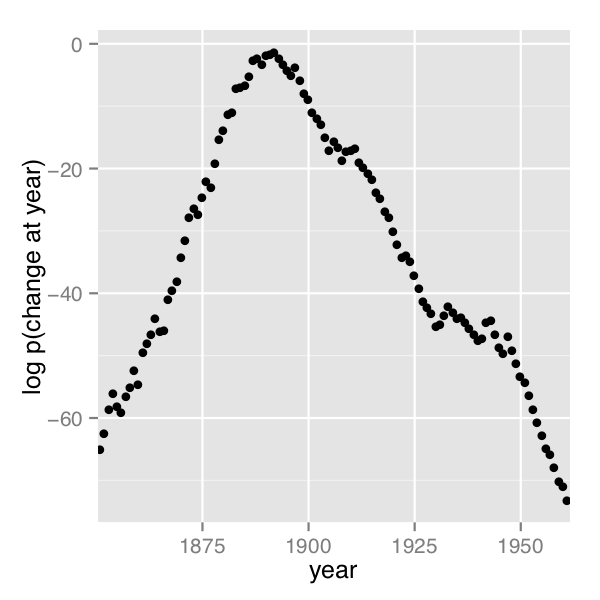
\includegraphics[width=0.7\linewidth]{./img/change-point-posterior} 

}

\caption{Analytical change-point posterior}\label{fig:unnamed-chunk-10}
\end{figure}

The frequency of change points generated by sampling the discrete change
points.

\begin{figure}

{\centering 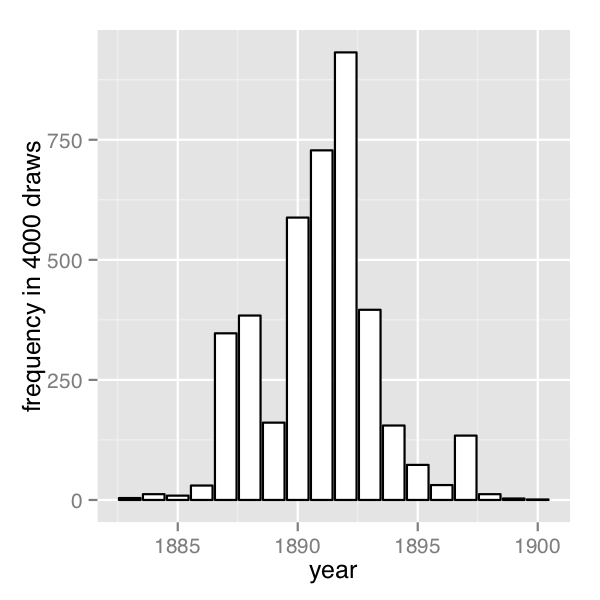
\includegraphics[width=0.7\linewidth]{./img/s-discrete-posterior} 

}

\caption{Sampled change-point posterior}\label{fig:unnamed-chunk-11}
\end{figure}

In order their range of estimates be visible, the first plot is on the log
scale and the second plot on the linear scale; note the narrower range
of years in the second plot resulting from sampling. The posterior
mean of \(s\) is roughly 1891.

\hypertarget{discrete-sampling}{%
\subsection*{Discrete sampling}\label{discrete-sampling}}
\addcontentsline{toc}{subsection}{Discrete sampling}

The generated quantities block may be used to draw discrete parameter
values using the built-in pseudo-random number generators. For
example, with \texttt{lp} defined as above, the following program
draws a random value for \texttt{s} at every iteration.

\begin{Shaded}
\begin{Highlighting}[]
\KeywordTok{generated quantities}\NormalTok{ \{}
  \DataTypeTok{int}\NormalTok{\textless{}}\KeywordTok{lower}\NormalTok{=}\DecValTok{1}\NormalTok{, }\KeywordTok{upper}\NormalTok{=T\textgreater{} s;}
\NormalTok{  s = categorical\_logit\_rng(lp);}
\NormalTok{\}}
\end{Highlighting}
\end{Shaded}

A posterior histogram of draws for \(s\) is shown on the second change
point posterior figure above.

Compared to working in terms of expectations, discrete sampling is
highly inefficient, especially for tails of distributions, so this
approach should only be used if draws from a distribution are
explicitly required. Otherwise, expectations should be computed in
the generated quantities block based on the posterior distribution for
\texttt{s} given by \texttt{softmax(lp)}.

\hypertarget{posterior-covariance}{%
\subsection*{Posterior covariance}\label{posterior-covariance}}
\addcontentsline{toc}{subsection}{Posterior covariance}

The discrete sample generated for \(s\) can be used to calculate
covariance with other parameters. Although the sampling approach is
straightforward, it is more statistically efficient (in the sense of
requiring far fewer iterations for the same degree of accuracy) to
calculate these covariances in expectation using \texttt{lp}.

\hypertarget{multiple-change-points}{%
\subsection*{Multiple change points}\label{multiple-change-points}}
\addcontentsline{toc}{subsection}{Multiple change points}

There is no obstacle in principle to allowing multiple change points.
The only issue is that computation increases from linear to quadratic
in marginalizing out two change points, cubic for three change points,
and so on. There are three parameters, \texttt{e}, \texttt{m}, and
\texttt{l}, and two loops for the change point and then one over time,
with log densities being stored in a matrix.

\begin{Shaded}
\begin{Highlighting}[]
\DataTypeTok{matrix}\NormalTok{[T, T] lp;}
\NormalTok{lp = rep\_matrix(log\_unif, T);}
\ControlFlowTok{for}\NormalTok{ (s1 }\ControlFlowTok{in} \DecValTok{1}\NormalTok{:T) \{}
  \ControlFlowTok{for}\NormalTok{ (s2 }\ControlFlowTok{in} \DecValTok{1}\NormalTok{:T) \{}
    \ControlFlowTok{for}\NormalTok{ (t }\ControlFlowTok{in} \DecValTok{1}\NormalTok{:T) \{}
\NormalTok{      lp[s1,s2] = lp[s1,s2]}
\NormalTok{        + poisson\_lpmf(D[t] | t \textless{} s1 ? e : (t \textless{} s2 ? m : l));}
\NormalTok{    \}}
\NormalTok{  \}}
\NormalTok{\}}
\end{Highlighting}
\end{Shaded}

The matrix can then be converted back to a vector using
\texttt{to\_vector} before being passed to \texttt{log\_sum\_exp}.

\hypertarget{mark-recapture-models}{%
\section{Mark-recapture models}\label{mark-recapture-models}}

A widely applied field method in ecology is to capture (or sight)
animals, mark them (e.g., by tagging), then release them. This
process is then repeated one or more times, and is often done for
populations on an ongoing basis. The resulting data may be used to
estimate population size.

The first subsection describes a simple mark-recapture model that does
not involve any latent discrete parameters. The following subsections
describes the Cormack-Jolly-Seber model, which involves latent
discrete parameters for animal death.

\hypertarget{simple-mark-recapture-model}{%
\subsection*{Simple mark-recapture model}\label{simple-mark-recapture-model}}
\addcontentsline{toc}{subsection}{Simple mark-recapture model}

In the simplest case, a one-stage mark-recapture study produces the
following data

\begin{itemize}
\tightlist
\item
  \(M\) : number of animals marked in first capture,
\item
  \(C\) : number animals in second capture, and
\item
  \(R\) : number of marked animals in second capture.
\end{itemize}

The estimand of interest is

\begin{itemize}
\tightlist
\item
  \(N\) : number of animals in the population.
\end{itemize}

Despite the notation, the model will take \(N\) to be a continuous
parameter; just because the population must be finite doesn't mean the
parameter representing it must be. The parameter will be used to
produce a real-valued estimate of the population size.

The Lincoln-Petersen (\protect\hyperlink{ref-Lincoln:1930}{Lincoln 1930}; \protect\hyperlink{ref-Petersen:1896}{Petersen 1896}) method for
estimating population size is
\[
\hat{N} = \frac{M C}{R}.
\]

This population estimate would arise from a probabilistic model in
which the number of recaptured animals is distributed binomially,
\[
R \sim \textsf{binomial}(C, M / N)
\]
given the total number of animals captured in the second round (\(C\))
with a recapture probability of \(M/N\), the fraction of the total
population \(N\) marked in the first round.

\begin{Shaded}
\begin{Highlighting}[]
\KeywordTok{data}\NormalTok{ \{}
  \DataTypeTok{int}\NormalTok{\textless{}}\KeywordTok{lower}\NormalTok{=}\DecValTok{0}\NormalTok{\textgreater{} M;}
  \DataTypeTok{int}\NormalTok{\textless{}}\KeywordTok{lower}\NormalTok{=}\DecValTok{0}\NormalTok{\textgreater{} C;}
  \DataTypeTok{int}\NormalTok{\textless{}}\KeywordTok{lower}\NormalTok{=}\DecValTok{0}\NormalTok{, }\KeywordTok{upper}\NormalTok{=min(M, C)\textgreater{} R;}
\NormalTok{\}}
\KeywordTok{parameters}\NormalTok{ \{}
  \DataTypeTok{real}\NormalTok{\textless{}}\KeywordTok{lower}\NormalTok{=(C {-} R + M)\textgreater{} N;}
\NormalTok{\}}
\KeywordTok{model}\NormalTok{ \{}
\NormalTok{  R \textasciitilde{} binomial(C, M / N);}
\NormalTok{\}}
\end{Highlighting}
\end{Shaded}

A probabilistic formulation of the Lincoln-Petersen
estimator for population size based on data from a one-step
mark-recapture study. The lower bound on \(N\) is necessary to
efficiently eliminate impossible values.

The probabilistic variant of the Lincoln-Petersen estimator can be
directly coded in Stan as shown in the Lincon-Petersen model figure.
The Lincoln-Petersen estimate is the maximum likelihood estimate (MLE)
for this model.

To ensure the MLE is the Lincoln-Petersen estimate, an improper
uniform prior for \(N\) is used; this could (and should) be replaced
with a more informative prior if possible, based on knowledge of the
population under study.

The one tricky part of the model is the lower bound \(C - R + M\) placed
on the population size \(N\). Values below this bound are impossible
because it is otherwise not possible to draw \(R\) samples out of the
\(C\) animals recaptured. Implementing this lower bound is necessary to
ensure sampling and optimization can be carried out in an
unconstrained manner with unbounded support for parameters on the
transformed (unconstrained) space. The lower bound in the declaration
for \(C\) implies a variable transform
\(f : (C-R+M,\infty) \rightarrow (-\infty,+\infty)\) defined by
\(f(N) = \log(N - (C - R + M))\); the reference manual contains full
details of all constrained parameter transforms.

\hypertarget{cormack-jolly-seber-with-discrete-parameter}{%
\subsection*{Cormack-Jolly-Seber with discrete parameter}\label{cormack-jolly-seber-with-discrete-parameter}}
\addcontentsline{toc}{subsection}{Cormack-Jolly-Seber with discrete parameter}

The Cormack-Jolly-Seber (CJS) model (\protect\hyperlink{ref-Cormack:1964}{Cormack 1964}; \protect\hyperlink{ref-Jolly:1965}{Jolly 1965}; \protect\hyperlink{ref-Seber:1965}{Seber 1965})
is an open-population model in which the population may change over time
due to death; the presentation here draws heavily on Schofield (\protect\hyperlink{ref-Schofield:2007}{2007}).

The basic data are

\begin{itemize}
\tightlist
\item
  \(I\): number of individuals,
\item
  \(T\): number of capture periods, and
\item
  \(y_{i,t}\): Boolean indicating if individual \(i\) was captured at
  time \(t\).
\end{itemize}

Each individual is assumed to have been captured at least once because
an individual only contributes information conditionally after they
have been captured the first time.

There are two Bernoulli parameters in the model,

\begin{itemize}
\tightlist
\item
  \(\phi_t\) : probability that animal alive at time \(t\) survives
  until \(t + 1\) and
\item
  \(p_t\) : probability that animal alive at time \(t\) is captured at
  time \(t\).
\end{itemize}

These parameters will both be given uniform priors, but information
should be used to tighten these priors in practice.

The CJS model also employs a latent discrete parameter \(z_{i,t}\)
indicating for each individual \(i\) whether it is alive at time \(t\),
distributed as
\[
z_{i,t} \sim \mathsf{Bernoulli}(z_{i,t-1} \; ? \; 0 \: : \: \phi_{t-1}).
\]

The conditional prevents the model positing zombies; once an animal is
dead, it stays dead. The data distribution is then simple to express
conditional on \(z\) as
\[
y_{i,t} \sim \mathsf{Bernoulli}(z_{i,t} \; ? \; 0 \: : \: p_t).
\]

The conditional enforces the constraint that dead animals cannot be captured.

\hypertarget{collective-cormack-jolly-seber-model}{%
\subsection*{Collective Cormack-Jolly-Seber model}\label{collective-cormack-jolly-seber-model}}
\addcontentsline{toc}{subsection}{Collective Cormack-Jolly-Seber model}

This subsection presents an implementation of the model in terms of
counts for different history profiles for individuals over three
capture times. It assumes exchangeability of the animals in that each
is assigned the same capture and survival probabilities.

In order to ease the marginalization of the latent discrete parameter
\(z_{i,t}\), the Stan models rely on a derived quantity \(\chi_t\) for
the probability that an individual is never captured again if it is
alive at time \(t\) (if it is dead, the recapture probability is zero).
this quantity is defined recursively by
\[
\chi_t
=
\begin{cases}
1 & \quad\text{if } t = T \\
(1 - \phi_t) + \phi_t (1 - p_{t+1}) \chi_{t+1}
  & \quad\text{if } t < T
\end{cases}
\]

The base case arises because if an animal was captured in the last
time period, the probability it is never captured again is 1 because
there are no more capture periods. The recursive case defining
\(\chi_{t}\) in terms of \(\chi_{t+1}\) involves two possibilities: (1)
not surviving to the next time period, with probability \((1 - \phi_t)\), or (2) surviving to the next time period with probability
\(\phi_t\), not being captured in the next time period with probability
\((1 - p_{t+1})\), and not being captured again after being alive in
period \(t+1\) with probability \(\chi_{t+1}\).

With three capture times, there are eight captured/not-captured
profiles an individual may have. These may be naturally coded as
binary numbers as follows.

\begin{table}
\centering
\begin{tabular}{ccccc}
\toprule
\multicolumn{1}{c}{} & \multicolumn{3}{c}{captures} & \multicolumn{1}{c}{} \\
\cmidrule(l{3pt}r{3pt}){2-4}
profile & 1 & 2 & 3 & probability\\
\midrule
0 & $-$ & $-$ & $-$ & n/a\\
1 & $-$ & $-$ & $+$ & n/a\\
2 & $-$ & $+$ & $-$ & $\chi_2$\\
3 & $-$ & $+$ & $+$ & $\phi_2 \, p_3$\\
4 & $+$ & $-$ & $-$ & $\chi_1$\\
\addlinespace
5 & $+$ & $-$ & $+$ & $\phi_1 \, (1 - p_2) \, \phi_2 \, p_3$\\
6 & $+$ & $+$ & $-$ & $\phi_1 \, p_2 \, \chi_2$\\
7 & $+$ & $+$ & $+$ & $\phi_1 \, p_2 \, \phi_2 \, p_3$\\
\bottomrule
\end{tabular}
\end{table}

History 0, for animals that are never captured, is unobservable
because only animals that are captured are observed. History 1, for
animals that are only captured in the last round, provides no
information for the CJS model, because capture/non-capture status is
only informative when conditioned on earlier captures. For the
remaining cases, the contribution to the likelihood is provided in the
final column.

By defining these probabilities in terms of \(\chi\) directly, there is
no need for a latent binary parameter indicating whether an animal is
alive at time \(t\) or not. The definition of \(\chi\) is typically used
to define the likelihood (i.e., marginalize out the latent discrete
parameter) for the CJS model (\protect\hyperlink{ref-Schofield:2007}{Schofield 2007}).

The Stan model defines \(\chi\) as a transformed parameter based on
parameters \(\phi\) and \(p\). In the model block, the log probability is
incremented for each history based on its count. This second step is
similar to collecting Bernoulli observations into a binomial or
categorical observations into a multinomial, only it is coded directly
in the Stan program using \texttt{target\ +=} rather than
being part of a built-in probability function.

The following is the Stan program for the Cormack-Jolly-Seber
mark-recapture model that considers counts of individuals with
observation histories of being observed or not in three capture
periods

\begin{Shaded}
\begin{Highlighting}[]
\KeywordTok{data}\NormalTok{ \{}
  \DataTypeTok{array}\NormalTok{[}\DecValTok{7}\NormalTok{] }\DataTypeTok{int}\NormalTok{\textless{}}\KeywordTok{lower}\NormalTok{=}\DecValTok{0}\NormalTok{\textgreater{} history;}
\NormalTok{\}}
\KeywordTok{parameters}\NormalTok{ \{}
  \DataTypeTok{array}\NormalTok{[}\DecValTok{2}\NormalTok{] }\DataTypeTok{real}\NormalTok{\textless{}}\KeywordTok{lower}\NormalTok{=}\DecValTok{0}\NormalTok{, }\KeywordTok{upper}\NormalTok{=}\DecValTok{1}\NormalTok{\textgreater{} phi;}
  \DataTypeTok{array}\NormalTok{[}\DecValTok{3}\NormalTok{] }\DataTypeTok{real}\NormalTok{\textless{}}\KeywordTok{lower}\NormalTok{=}\DecValTok{0}\NormalTok{, }\KeywordTok{upper}\NormalTok{=}\DecValTok{1}\NormalTok{\textgreater{} p;}
\NormalTok{\}}
\KeywordTok{transformed parameters}\NormalTok{ \{}
  \DataTypeTok{array}\NormalTok{[}\DecValTok{2}\NormalTok{] }\DataTypeTok{real}\NormalTok{\textless{}}\KeywordTok{lower}\NormalTok{=}\DecValTok{0}\NormalTok{, }\KeywordTok{upper}\NormalTok{=}\DecValTok{1}\NormalTok{\textgreater{} chi;}
\NormalTok{  chi[}\DecValTok{2}\NormalTok{] = (}\DecValTok{1}\NormalTok{ {-} phi[}\DecValTok{2}\NormalTok{]) + phi[}\DecValTok{2}\NormalTok{] * (}\DecValTok{1}\NormalTok{ {-} p[}\DecValTok{3}\NormalTok{]);}
\NormalTok{  chi[}\DecValTok{1}\NormalTok{] = (}\DecValTok{1}\NormalTok{ {-} phi[}\DecValTok{1}\NormalTok{]) + phi[}\DecValTok{1}\NormalTok{] * (}\DecValTok{1}\NormalTok{ {-} p[}\DecValTok{2}\NormalTok{]) * chi[}\DecValTok{2}\NormalTok{];}
\NormalTok{\}}
\KeywordTok{model}\NormalTok{ \{}
  \KeywordTok{target +=}\NormalTok{ history[}\DecValTok{2}\NormalTok{] * log(chi[}\DecValTok{2}\NormalTok{]);}
  \KeywordTok{target +=}\NormalTok{ history[}\DecValTok{3}\NormalTok{] * (log(phi[}\DecValTok{2}\NormalTok{]) + log(p[}\DecValTok{3}\NormalTok{]));}
  \KeywordTok{target +=}\NormalTok{ history[}\DecValTok{4}\NormalTok{] * (log(chi[}\DecValTok{1}\NormalTok{]));}
  \KeywordTok{target +=}\NormalTok{ history[}\DecValTok{5}\NormalTok{] * (log(phi[}\DecValTok{1}\NormalTok{]) + log1m(p[}\DecValTok{2}\NormalTok{])}
\NormalTok{                            + log(phi[}\DecValTok{2}\NormalTok{]) + log(p[}\DecValTok{3}\NormalTok{]));}
  \KeywordTok{target +=}\NormalTok{ history[}\DecValTok{6}\NormalTok{] * (log(phi[}\DecValTok{1}\NormalTok{]) + log(p[}\DecValTok{2}\NormalTok{])}
\NormalTok{                            + log(chi[}\DecValTok{2}\NormalTok{]));}
  \KeywordTok{target +=}\NormalTok{ history[}\DecValTok{7}\NormalTok{] * (log(phi[}\DecValTok{1}\NormalTok{]) + log(p[}\DecValTok{2}\NormalTok{])}
\NormalTok{                            + log(phi[}\DecValTok{2}\NormalTok{]) + log(p[}\DecValTok{3}\NormalTok{]));}
\NormalTok{\}}
\KeywordTok{generated quantities}\NormalTok{ \{}
  \DataTypeTok{real}\NormalTok{\textless{}}\KeywordTok{lower}\NormalTok{=}\DecValTok{0}\NormalTok{, }\KeywordTok{upper}\NormalTok{=}\DecValTok{1}\NormalTok{\textgreater{} beta3;}
\NormalTok{  beta3 = phi[}\DecValTok{2}\NormalTok{] * p[}\DecValTok{3}\NormalTok{];}
\NormalTok{\}}
\end{Highlighting}
\end{Shaded}

\hypertarget{identifiability-1}{%
\subsubsection*{Identifiability}\label{identifiability-1}}
\addcontentsline{toc}{subsubsection}{Identifiability}

The parameters \(\phi_2\) and \(p_3\), the probability of death at time 2
and probability of capture at time 3 are not identifiable, because both
may be used to account for lack of capture at time 3. Their product,
\(\beta_3 = \phi_2 \, p_3\), is identified. The Stan model defines
\texttt{beta3} as a generated quantity. Unidentified parameters pose a
problem for Stan's samplers' adaptation. Although the problem posed
for adaptation is mild here because the parameters are bounded and
thus have proper uniform priors, it would be better to formulate an
identified parameterization. One way to do this would be to formulate
a hierarchical model for the \(p\) and \(\phi\) parameters.

\hypertarget{individual-cormack-jolly-seber-model}{%
\subsection*{Individual Cormack-Jolly-Seber model}\label{individual-cormack-jolly-seber-model}}
\addcontentsline{toc}{subsection}{Individual Cormack-Jolly-Seber model}

This section presents a version of the Cormack-Jolly-Seber (CJS) model
cast at the individual level rather than collectively as in the
previous subsection. It also extends the model to allow an arbitrary
number of time periods. The data will consist of the number \(T\) of
capture events, the number \(I\) of individuals, and a boolean flag
\(y_{i,t}\) indicating if individual \(i\) was observed at time \(t\). In
Stan,

\begin{Shaded}
\begin{Highlighting}[]
\KeywordTok{data}\NormalTok{ \{}
  \DataTypeTok{int}\NormalTok{\textless{}}\KeywordTok{lower}\NormalTok{=}\DecValTok{2}\NormalTok{\textgreater{} T;}
  \DataTypeTok{int}\NormalTok{\textless{}}\KeywordTok{lower}\NormalTok{=}\DecValTok{0}\NormalTok{\textgreater{} I;}
  \DataTypeTok{array}\NormalTok{[I, T] }\DataTypeTok{int}\NormalTok{\textless{}}\KeywordTok{lower}\NormalTok{=}\DecValTok{0}\NormalTok{, }\KeywordTok{upper}\NormalTok{=}\DecValTok{1}\NormalTok{\textgreater{} y;}
\NormalTok{\}}
\end{Highlighting}
\end{Shaded}

The advantages to the individual-level model is that it becomes
possible to add individual ``random effects'' that affect survival or
capture probability, as well as to avoid the combinatorics involved in
unfolding \(2^T\) observation histories for \(T\) capture times.

\hypertarget{utility-functions}{%
\subsubsection*{Utility functions}\label{utility-functions}}
\addcontentsline{toc}{subsubsection}{Utility functions}

The individual CJS model is written involves several function
definitions. The first two are used in the transformed data block to
compute the first and last time period in which an animal was
captured.\footnote{An alternative would be to compute this on the outside and feed it into the Stan model as preprocessed data. Yet another alternative encoding would be a sparse one recording only the capture events along with their time and identifying the individual captured.}

\begin{Shaded}
\begin{Highlighting}[]
\KeywordTok{functions}\NormalTok{ \{}
  \DataTypeTok{int}\NormalTok{ first\_capture(}\DataTypeTok{array}\NormalTok{[] }\DataTypeTok{int}\NormalTok{ y\_i) \{}
    \ControlFlowTok{for}\NormalTok{ (k }\ControlFlowTok{in} \DecValTok{1}\NormalTok{:size(y\_i)) \{}
      \ControlFlowTok{if}\NormalTok{ (y\_i[k]) \{}
        \ControlFlowTok{return}\NormalTok{ k;}
\NormalTok{      \}}
\NormalTok{    \}}
    \ControlFlowTok{return} \DecValTok{0}\NormalTok{;}
\NormalTok{  \}}
  \DataTypeTok{int}\NormalTok{ last\_capture(}\DataTypeTok{array}\NormalTok{[] }\DataTypeTok{int}\NormalTok{ y\_i) \{}
    \ControlFlowTok{for}\NormalTok{ (k\_rev }\ControlFlowTok{in} \DecValTok{0}\NormalTok{:(size(y\_i) {-} }\DecValTok{1}\NormalTok{)) \{}
      \DataTypeTok{int}\NormalTok{ k;}
\NormalTok{      k = size(y\_i) {-} k\_rev;}
      \ControlFlowTok{if}\NormalTok{ (y\_i[k]) \{}
        \ControlFlowTok{return}\NormalTok{ k;}
\NormalTok{      \}}
\NormalTok{    \}}
    \ControlFlowTok{return} \DecValTok{0}\NormalTok{;}
\NormalTok{  \}}
  \CommentTok{// ...}
\NormalTok{\}}
\end{Highlighting}
\end{Shaded}

These two functions are used to define the first and last capture time
for each individual in the transformed data block.\footnote{Both functions return 0 if the individual represented by the input array was never captured. Individuals with no captures are not relevant for estimating the model because all probability statements are conditional on earlier captures. Typically they would be removed from the data, but the program allows them to be included even though they make not contribution to the log probability function.}

\begin{Shaded}
\begin{Highlighting}[]
\KeywordTok{transformed data}\NormalTok{ \{}
  \DataTypeTok{array}\NormalTok{[I] }\DataTypeTok{int}\NormalTok{\textless{}}\KeywordTok{lower}\NormalTok{=}\DecValTok{0}\NormalTok{, }\KeywordTok{upper}\NormalTok{=T\textgreater{} first;}
  \DataTypeTok{array}\NormalTok{[I] }\DataTypeTok{int}\NormalTok{\textless{}}\KeywordTok{lower}\NormalTok{=}\DecValTok{0}\NormalTok{, }\KeywordTok{upper}\NormalTok{=T\textgreater{} last;}
  \DataTypeTok{vector}\NormalTok{\textless{}}\KeywordTok{lower}\NormalTok{=}\DecValTok{0}\NormalTok{, }\KeywordTok{upper}\NormalTok{=I\textgreater{}[T] n\_captured;}
  \ControlFlowTok{for}\NormalTok{ (i }\ControlFlowTok{in} \DecValTok{1}\NormalTok{:I) \{}
\NormalTok{    first[i] = first\_capture(y[i]);}
\NormalTok{  \}}
  \ControlFlowTok{for}\NormalTok{ (i }\ControlFlowTok{in} \DecValTok{1}\NormalTok{:I) \{}
\NormalTok{    last[i] = last\_capture(y[i]);}
\NormalTok{  \}}
\NormalTok{  n\_captured = rep\_vector(}\DecValTok{0}\NormalTok{, T);}
  \ControlFlowTok{for}\NormalTok{ (t }\ControlFlowTok{in} \DecValTok{1}\NormalTok{:T) \{}
    \ControlFlowTok{for}\NormalTok{ (i }\ControlFlowTok{in} \DecValTok{1}\NormalTok{:I) \{}
      \ControlFlowTok{if}\NormalTok{ (y[i, t]) \{}
\NormalTok{        n\_captured[t] = n\_captured[t] + }\DecValTok{1}\NormalTok{;}
\NormalTok{      \}}
\NormalTok{    \}}
\NormalTok{  \}}
\NormalTok{\}}
\end{Highlighting}
\end{Shaded}

The transformed data block also defines \texttt{n\_captured{[}t{]}}, which is
the total number of captures at time \texttt{t}. The variable
\texttt{n\_captured} is defined as a vector instead of an integer array
so that it can be used in an elementwise vector operation in the generated
quantities block to model the population estimates at each time point.

The parameters and transformed parameters are as before, but now there
is a function definition for computing the entire vector \texttt{chi}, the
probability that if an individual is alive at \texttt{t} that it will
never be captured again.

\begin{Shaded}
\begin{Highlighting}[]
\KeywordTok{parameters}\NormalTok{ \{}
  \DataTypeTok{vector}\NormalTok{\textless{}}\KeywordTok{lower}\NormalTok{=}\DecValTok{0}\NormalTok{, }\KeywordTok{upper}\NormalTok{=}\DecValTok{1}\NormalTok{\textgreater{}[T {-} }\DecValTok{1}\NormalTok{] phi;}
  \DataTypeTok{vector}\NormalTok{\textless{}}\KeywordTok{lower}\NormalTok{=}\DecValTok{0}\NormalTok{, }\KeywordTok{upper}\NormalTok{=}\DecValTok{1}\NormalTok{\textgreater{}[T] p;}
\NormalTok{\}}
\KeywordTok{transformed parameters}\NormalTok{ \{}
  \DataTypeTok{vector}\NormalTok{\textless{}}\KeywordTok{lower}\NormalTok{=}\DecValTok{0}\NormalTok{, }\KeywordTok{upper}\NormalTok{=}\DecValTok{1}\NormalTok{\textgreater{}[T] chi;}
\NormalTok{  chi = prob\_uncaptured(T, p, phi);}
\NormalTok{\}}
\end{Highlighting}
\end{Shaded}

The definition of \texttt{prob\_uncaptured}, from the functions block,
is

\begin{Shaded}
\begin{Highlighting}[]
\KeywordTok{functions}\NormalTok{ \{}
  \CommentTok{// ...}
  \DataTypeTok{vector}\NormalTok{ prob\_uncaptured(}\DataTypeTok{int}\NormalTok{ T, }\DataTypeTok{vector}\NormalTok{ p, }\DataTypeTok{vector}\NormalTok{ phi) \{}
    \DataTypeTok{vector}\NormalTok{[T] chi;}
\NormalTok{    chi[T] = }\FloatTok{1.0}\NormalTok{;}
    \ControlFlowTok{for}\NormalTok{ (t }\ControlFlowTok{in} \DecValTok{1}\NormalTok{:(T {-} }\DecValTok{1}\NormalTok{)) \{}
      \DataTypeTok{int}\NormalTok{ t\_curr;}
      \DataTypeTok{int}\NormalTok{ t\_next;}
\NormalTok{      t\_curr = T {-} t;}
\NormalTok{      t\_next = t\_curr + }\DecValTok{1}\NormalTok{;}
\NormalTok{      chi[t\_curr] = (}\DecValTok{1}\NormalTok{ {-} phi[t\_curr])}
\NormalTok{                     + phi[t\_curr]}
\NormalTok{                       * (}\DecValTok{1}\NormalTok{ {-} p[t\_next])}
\NormalTok{                       * chi[t\_next];}
\NormalTok{    \}}
    \ControlFlowTok{return}\NormalTok{ chi;}
\NormalTok{  \}}
\NormalTok{\}}
\end{Highlighting}
\end{Shaded}

The function definition directly follows the mathematical definition
of \(\chi_t\), unrolling the recursion into an iteration and
defining the elements of \texttt{chi} from \texttt{T} down to 1.

\hypertarget{the-model}{%
\subsubsection*{The model}\label{the-model}}
\addcontentsline{toc}{subsubsection}{The model}

Given the precomputed quantities, the model block directly encodes the
CJS model's log likelihood function. All parameters are left with
their default uniform priors and the model simply encodes the log
probability of the observations \texttt{q} given the parameters \texttt{p}
and \texttt{phi} as well as the transformed parameter \texttt{chi} defined
in terms of \texttt{p} and \texttt{phi}.

\begin{Shaded}
\begin{Highlighting}[]
\KeywordTok{model}\NormalTok{ \{}
  \ControlFlowTok{for}\NormalTok{ (i }\ControlFlowTok{in} \DecValTok{1}\NormalTok{:I) \{}
    \ControlFlowTok{if}\NormalTok{ (first[i] \textgreater{} }\DecValTok{0}\NormalTok{) \{}
      \ControlFlowTok{for}\NormalTok{ (t }\ControlFlowTok{in}\NormalTok{ (first[i]+}\DecValTok{1}\NormalTok{):last[i]) \{}
        \DecValTok{1}\NormalTok{ \textasciitilde{} bernoulli(phi[t {-} }\DecValTok{1}\NormalTok{]);}
\NormalTok{        y[i, t] \textasciitilde{} bernoulli(p[t]);}
\NormalTok{      \}}
      \DecValTok{1}\NormalTok{ \textasciitilde{} bernoulli(chi[last[i]]);}
\NormalTok{    \}}
\NormalTok{  \}}
\NormalTok{\}}
\end{Highlighting}
\end{Shaded}

The outer loop is over individuals, conditional skipping individuals
\texttt{i} which are never captured. The never-captured check depends
on the convention of the first-capture and last-capture functions
returning 0 for \texttt{first} if an individual is never captured.

The inner loop for individual \texttt{i} first increments the log
probability based on the survival of the individual with probability
\texttt{phi{[}t\ -\ 1{]}}. The outcome of 1 is fixed because the individual
must survive between the first and last capture (i.e., no zombies).
The loop starts after the first capture, because all
information in the CJS model is conditional on the first capture.

In the inner loop, the observed capture status \texttt{y{[}i,\ t{]}} for
individual \texttt{i} at time \texttt{t} has a Bernoulli distribution
based on the capture probability \texttt{p{[}t{]}} at time \texttt{t}.

After the inner loop, the probability of an animal never being seen
again after being observed at time \texttt{last{[}i{]}} is included, because
\texttt{last{[}i{]}} was defined to be the last time period in which animal
\texttt{i} was observed.

\hypertarget{identified-parameters}{%
\subsubsection*{Identified parameters}\label{identified-parameters}}
\addcontentsline{toc}{subsubsection}{Identified parameters}

As with the collective model described in the previous subsection,
this model does not identify \texttt{phi{[}T\ -\ 1{]}} and \texttt{p{[}T{]}}, but
does identify their product, \texttt{beta}. Thus \texttt{beta} is defined
as a generated quantity to monitor convergence and report.

\begin{Shaded}
\begin{Highlighting}[]
\KeywordTok{generated quantities}\NormalTok{ \{}
  \DataTypeTok{real}\NormalTok{ beta;}
  \CommentTok{// ...}

\NormalTok{  beta = phi[T {-} }\DecValTok{1}\NormalTok{] * p[T];}
  \CommentTok{// ...}
\NormalTok{\}}
\end{Highlighting}
\end{Shaded}

The parameter \texttt{p{[}1{]}} is also not modeled and will just be uniform
between 0 and 1. A more finely articulated model might have a
hierarchical or time-series component, in which case \texttt{p{[}1{]}} would
be an unknown initial condition and both \texttt{phi{[}T\ -\ 1{]}} and
\texttt{p{[}T{]}} could be identified.

\hypertarget{population-size-estimates}{%
\subsubsection*{Population size estimates}\label{population-size-estimates}}
\addcontentsline{toc}{subsubsection}{Population size estimates}

The generated quantities also calculates an estimate of the population
mean at each time \texttt{t} in the same way as in the simple
mark-recapture model as the number of individuals captured at time
\texttt{t} divided by the probability of capture at time \texttt{t}. This
is done with the elementwise division operation for vectors
(\texttt{./}) in the generated quantities block.

\begin{Shaded}
\begin{Highlighting}[]
\KeywordTok{generated quantities}\NormalTok{ \{}
  \CommentTok{// ...}
  \DataTypeTok{vector}\NormalTok{\textless{}}\KeywordTok{lower}\NormalTok{=}\DecValTok{0}\NormalTok{\textgreater{}[T] pop;}
  \CommentTok{// ...}
\NormalTok{  pop = n\_captured ./ p;}
\NormalTok{  pop[}\DecValTok{1}\NormalTok{] = {-}}\DecValTok{1}\NormalTok{;}
\NormalTok{\}}
\end{Highlighting}
\end{Shaded}

\hypertarget{generalizing-to-individual-effects}{%
\subsubsection*{Generalizing to individual effects}\label{generalizing-to-individual-effects}}
\addcontentsline{toc}{subsubsection}{Generalizing to individual effects}

All individuals are modeled as having the same capture probability,
but this model could be easily generalized to use a logistic
regression here based on individual-level inputs to be used as
predictors.

\hypertarget{data-coding-models.section}{%
\section{Data coding and diagnostic accuracy models}\label{data-coding-models.section}}

Although seemingly disparate tasks, the rating/coding/annotation of
items with categories and diagnostic testing for disease or other
conditions, share several characteristics which allow their statistical
properties to be modeled similarly.

\hypertarget{diagnostic-accuracy}{%
\subsection*{Diagnostic accuracy}\label{diagnostic-accuracy}}
\addcontentsline{toc}{subsection}{Diagnostic accuracy}

Suppose you have diagnostic tests for a condition of varying
sensitivity and specificity. Sensitivity is the probability a test
returns positive when the patient has the condition and specificity is
the probability that a test returns negative when the patient does not
have the condition. For example, mammograms and puncture biopsy tests
both test for the presence of breast cancer. Mammograms have high
sensitivity and low specificity, meaning lots of false positives,
whereas puncture biopsies are the opposite, with low sensitivity and
high specificity, meaning lots of false negatives.

There are several estimands of interest in such studies. An
epidemiological study may be interested in the prevalence of a kind of
infection, such as malaria, in a population. A test development study
might be interested in the diagnostic accuracy of a new test. A health
care worker performing tests might be interested in the disease status
of a particular patient.

\hypertarget{data-coding}{%
\subsection*{Data coding}\label{data-coding}}
\addcontentsline{toc}{subsection}{Data coding}

Humans are often given the task of coding (equivalently rating or
annotating) data. For example, journal or grant reviewers rate
submissions, a political study may code campaign commercials as to
whether they are attack ads or not, a natural language processing
study might annotate Tweets as to whether they are positive or
negative in overall sentiment, or a dentist looking at an X-ray
classifies a patient as having a cavity or not. In all of these
cases, the data coders play the role of the diagnostic tests and all
of the same estimands are in play --- data coder accuracy and bias,
true categories of items being coded, or the prevalence of various
categories of items in the data.

\hypertarget{noisy-categorical-measurement-model}{%
\subsection*{Noisy categorical measurement model}\label{noisy-categorical-measurement-model}}
\addcontentsline{toc}{subsection}{Noisy categorical measurement model}

In this section, only categorical ratings are considered, and the
challenge in the modeling for Stan is to marginalize out the discrete
parameters.

A. P. Dawid and Skene (\protect\hyperlink{ref-DawidSkene:1979}{1979}) introduce a noisy-measurement model for
coding and apply it in the epidemiological setting of coding what
doctors say about patient histories; the same model can be used
for diagnostic procedures.

\hypertarget{data-1}{%
\subsubsection*{Data}\label{data-1}}
\addcontentsline{toc}{subsubsection}{Data}

The data for the model consists of \(J\) raters (diagnostic tests), \(I\)
items (patients), and \(K\) categories (condition statuses) to annotate,
with \(y_{i, j} \in \{1, \dotsc, K\}\) being the rating provided by rater \(j\) for
item \(i\). In a diagnostic test setting for a particular condition,
the raters are diagnostic procedures and often \(K=2\), with values
signaling the presence or absence of the condition.\footnote{Diagnostic procedures are often ordinal, as in stages of cancer in oncological diagnosis or the severity of a cavity in dental diagnosis. Dawid and Skene's model may be used as is or naturally generalized for ordinal ratings using a latent continuous rating and cutpoints as in ordinal logistic regression.}

It is relatively straightforward to extend Dawid and Skene's model to
deal with the situation where not every rater rates each item exactly
once.

\hypertarget{model-parameters}{%
\subsection*{Model parameters}\label{model-parameters}}
\addcontentsline{toc}{subsection}{Model parameters}

The model is based on three parameters, the first of which is discrete:

\begin{itemize}
\tightlist
\item
  \(z_i\) : a value in \(\{1, \dotsc, K\}\) indicating the true category of item \(i\),
\item
  \(\pi\) : a \(K\)-simplex for the prevalence of the \(K\)
  categories in the population, and
\item
  \(\theta_{j,k}\) : a \(K\)-simplex for the response of annotator \(j\)
  to an item of true category \(k\).
\end{itemize}

\hypertarget{noisy-measurement-model}{%
\subsection*{Noisy measurement model}\label{noisy-measurement-model}}
\addcontentsline{toc}{subsection}{Noisy measurement model}

The true category of an item is assumed to be generated by a simple
categorical distribution based on item prevalence,
\[
z_i \sim \textsf{categorical}(\pi).
\]

The rating \(y_{i, j}\) provided for item \(i\) by rater \(j\) is modeled as
a categorical response of rater \(i\) to an item of category \(z_i\),\footnote{In the subscript, \(z_i\) is written as \(z[i]\) to improve legibility.}
\[
y_{i, j} \sim \textsf{categorical}(\theta_{j,\pi_{z[i]}}).
\]

\hypertarget{priors-and-hierarchical-modeling}{%
\subsubsection*{Priors and hierarchical modeling}\label{priors-and-hierarchical-modeling}}
\addcontentsline{toc}{subsubsection}{Priors and hierarchical modeling}

Dawid and Skene provided maximum likelihood estimates for \(\theta\) and
\(\pi\), which allows them to generate probability estimates for each \(z_i\).

To mimic Dawid and Skene's maximum likelihood model, the parameters
\(\theta_{j,k}\) and \(\pi\) can be given uniform priors over
\(K\)-simplexes. It is straightforward to generalize to Dirichlet
priors,
\[
\pi \sim \textsf{Dirichlet}(\alpha)
\]
and
\[
\theta_{j,k} \sim \textsf{Dirichlet}(\beta_k)
\]
with fixed hyperparameters \(\alpha\) (a vector) and \(\beta\) (a matrix
or array of vectors). The prior for \(\theta_{j,k}\) must be allowed to
vary in \(k\), so that, for instance, \(\beta_{k,k}\) is large enough to
allow the prior to favor better-than-chance annotators over random or
adversarial ones.

Because there are \(J\) coders, it would be natural to extend the model
to include a hierarchical prior for \(\beta\) and to partially pool the
estimates of coder accuracy and bias.

\hypertarget{marginalizing-out-the-true-category}{%
\subsubsection*{Marginalizing out the true category}\label{marginalizing-out-the-true-category}}
\addcontentsline{toc}{subsubsection}{Marginalizing out the true category}

Because the true category parameter \(z\) is discrete, it must be
marginalized out of the joint posterior in order to carry out sampling
or maximum likelihood estimation in Stan. The joint posterior factors
as
\[
p(y, \theta, \pi) = p(y \mid \theta,\pi) \, p(\pi) \, p(\theta),
\]
where \(p(y \mid \theta,\pi)\) is derived by marginalizing \(z\) out of
\[
p(z, y \mid \theta, \pi) =
\prod_{i=1}^I \left( \textsf{categorical}(z_i \mid \pi)
                     \prod_{j=1}^J
                     \textsf{categorical}(y_{i, j} \mid \theta_{j, z[i]})
              \right).
\]

This can be done item by item, with
\[
p(y \mid \theta, \pi) =
\prod_{i=1}^I \sum_{k=1}^K
  \left( \textsf{categorical}(k \mid \pi)
         \prod_{j=1}^J
         \textsf{categorical}(y_{i, j} \mid \theta_{j, k})
  \right).
\]

In the missing data model, only the observed labels would be used in
the inner product.

A. P. Dawid and Skene (\protect\hyperlink{ref-DawidSkene:1979}{1979}) derive exactly the same equation in their
Equation (2.7), required for the E-step in their expectation
maximization (EM) algorithm. Stan requires the marginalized
probability function on the log scale,
\begin{align*}
\log p(y \mid \theta, \pi)
 &= \sum_{i=1}^I \log \left( \sum_{k=1}^K \exp
    \left(\log \textsf{categorical}(k \mid \pi) \vphantom{\sum_{j=1}^J}\right.\right. 
    \left.\left. + \ \sum_{j=1}^J
           \log \textsf{categorical}(y_{i, j} \mid \theta_{j, k})
    \right) \right),
\end{align*}
which can be directly coded using Stan's built-in \texttt{log\_sum\_exp}
function.

\hypertarget{stan-implementation}{%
\subsection*{Stan implementation}\label{stan-implementation}}
\addcontentsline{toc}{subsection}{Stan implementation}

The Stan program for the Dawid and Skene model is provided below (\protect\hyperlink{ref-DawidSkene:1979}{A. P. Dawid and Skene 1979}).

\begin{Shaded}
\begin{Highlighting}[]
\KeywordTok{data}\NormalTok{ \{}
  \DataTypeTok{int}\NormalTok{\textless{}}\KeywordTok{lower}\NormalTok{=}\DecValTok{2}\NormalTok{\textgreater{} K;}
  \DataTypeTok{int}\NormalTok{\textless{}}\KeywordTok{lower}\NormalTok{=}\DecValTok{1}\NormalTok{\textgreater{} I;}
  \DataTypeTok{int}\NormalTok{\textless{}}\KeywordTok{lower}\NormalTok{=}\DecValTok{1}\NormalTok{\textgreater{} J;}

  \DataTypeTok{array}\NormalTok{[I, J] }\DataTypeTok{int}\NormalTok{\textless{}}\KeywordTok{lower}\NormalTok{=}\DecValTok{1}\NormalTok{, }\KeywordTok{upper}\NormalTok{=K\textgreater{} y;}

  \DataTypeTok{vector}\NormalTok{\textless{}}\KeywordTok{lower}\NormalTok{=}\DecValTok{0}\NormalTok{\textgreater{}[K] alpha;}
  \DataTypeTok{vector}\NormalTok{\textless{}}\KeywordTok{lower}\NormalTok{=}\DecValTok{0}\NormalTok{\textgreater{}[K] beta[K];}
\NormalTok{\}}
\KeywordTok{parameters}\NormalTok{ \{}
  \DataTypeTok{simplex}\NormalTok{[K] pi;}
  \DataTypeTok{array}\NormalTok{[J, K] }\DataTypeTok{simplex}\NormalTok{[K] theta;}
\NormalTok{\}}
\KeywordTok{transformed parameters}\NormalTok{ \{}
  \DataTypeTok{array}\NormalTok{[I] }\DataTypeTok{vector}\NormalTok{[K] log\_q\_z;}
  \ControlFlowTok{for}\NormalTok{ (i }\ControlFlowTok{in} \DecValTok{1}\NormalTok{:I) \{}
\NormalTok{    log\_q\_z[i] = log(pi);}
    \ControlFlowTok{for}\NormalTok{ (j }\ControlFlowTok{in} \DecValTok{1}\NormalTok{:J) \{}
      \ControlFlowTok{for}\NormalTok{ (k }\ControlFlowTok{in} \DecValTok{1}\NormalTok{:K) \{}
\NormalTok{        log\_q\_z[i, k] = log\_q\_z[i, k]}
\NormalTok{                         + log(theta[j, k, y[i, j]]);}
\NormalTok{      \}}
\NormalTok{    \}}
\NormalTok{  \}}
\NormalTok{\}}
\KeywordTok{model}\NormalTok{ \{}
\NormalTok{  pi \textasciitilde{} dirichlet(alpha);}
  \ControlFlowTok{for}\NormalTok{ (j }\ControlFlowTok{in} \DecValTok{1}\NormalTok{:J) \{}
    \ControlFlowTok{for}\NormalTok{ (k }\ControlFlowTok{in} \DecValTok{1}\NormalTok{:K) \{}
\NormalTok{      theta[j, k] \textasciitilde{} dirichlet(beta[k]);}
\NormalTok{    \}}
\NormalTok{  \}}

  \ControlFlowTok{for}\NormalTok{ (i }\ControlFlowTok{in} \DecValTok{1}\NormalTok{:I) \{}
    \KeywordTok{target +=}\NormalTok{ log\_sum\_exp(log\_q\_z[i]);}
\NormalTok{  \}}
\NormalTok{\}}
\end{Highlighting}
\end{Shaded}

The model marginalizes out the discrete parameter \(z\), storing the
unnormalized conditional probability \(\log q(z_i=k|\theta,\pi)\) in
\texttt{log\_q\_z{[}i,\ k{]}}.

The Stan model converges quickly and mixes well using NUTS starting at
diffuse initial points, unlike the equivalent model implemented with
Gibbs sampling over the discrete parameter. Reasonable weakly
informative priors are \(\alpha_k = 3\) and \(\beta_{k,k} = 2.5 K\) and
\(\beta_{k,k'} = 1\) if \(k \neq k'\). Taking \(\alpha\) and \(\beta_k\) to
be unit vectors and applying optimization will produce the same answer
as the expectation maximization (EM) algorithm of
A. P. Dawid and Skene (\protect\hyperlink{ref-DawidSkene:1979}{1979}).

\hypertarget{inference-for-the-true-category}{%
\subsubsection*{Inference for the true category}\label{inference-for-the-true-category}}
\addcontentsline{toc}{subsubsection}{Inference for the true category}

The quantity \texttt{log\_q\_z{[}i{]}} is defined as a transformed
parameter. It encodes the (unnormalized) log of \(p(z_i \mid \theta, \pi)\). Each iteration provides a value conditioned on that
iteration's values for \(\theta\) and \(\pi\). Applying the softmax
function to \texttt{log\_q\_z{[}i{]}} provides a simplex corresponding to
the probability mass function of \(z_i\) in the posterior. These may
be averaged across the iterations to provide the posterior probability
distribution over each \(z_i\).

\hypertarget{marginalization-mathematics.section}{%
\section{The mathematics of recovering marginalized parameters}\label{marginalization-mathematics.section}}

\hypertarget{introduction}{%
\subsection*{Introduction}\label{introduction}}
\addcontentsline{toc}{subsection}{Introduction}

This section describes in more detail the mathematics of statistical inference using the output of marginalized Stan models, such as those presented in the last three sections. It provides a mathematical explanation of why and how certain manipulations of Stan's output produce valid summaries of the posterior distribution when discrete parameters have been marginalized out of a statistical model. Ultimately, however, fully understanding the mathematics in this section is \emph{not} necessary to fit models with discrete parameters using Stan.

Throughout, the model under consideration consists of both continuous parameters, \(\Theta\), and discrete parameters, \(Z\). It is also assumed that \(Z\) can only take finitely many values, as is the case for all the models described in this chapter of the User's Guide. To simplify notation, any conditioning on data is suppressed in this section, except where specified. As with all Bayesian analyses, however, all inferences using models with marginalized parameters are made conditional on the observed data.

\hypertarget{estimating-expectations}{%
\subsection*{Estimating expectations}\label{estimating-expectations}}
\addcontentsline{toc}{subsection}{Estimating expectations}

When performing Bayesian inference, interest often centers on estimating some (constant) low-dimensional summary statistics of the posterior distribution. Mathematically, we are interested in estimating \(\mu\), say, where \(\mu = \mathbb{E}[g(\Theta, Z)]\) and \(g(\cdot)\) is an arbitrary function. An example of such a quantity is \(\mathbb{E}[\Theta]\), the posterior mean of the continuous parameters, where we would take \(g(\theta, z) = \theta\). To estimate \(\mu\) the most common approach is to sample a series of values, at least approximately, from the posterior distribution of the parameters of interest. The numerical values of these draws can then be used to calculate the quantities of interest. Often, this process of calculation is trivial, but more care is required when working with marginalized posteriors as we describe in this section.

If both \(\Theta\) and \(Z\) were continuous, Stan could be used to sample \(M\) draws from the joint posterior \(p_{\Theta, Z}(\theta, z)\) and then estimate \(\mu\) with
\[   
\hat{\mu} = \frac{1}{M} \sum_{i = 1}^M {g(\theta^{(i)}, z^{(i)})}.
\]
Given \(Z\) is discrete, however, Stan cannot be used to sample from the joint posterior (or even to do optimization). Instead, as outlined in the previous sections describing specific models, the user can first marginalize out \(Z\) from the joint posterior to give the marginalized posterior \(p_\Theta(\theta)\). This marginalized posterior can then be implemented in Stan as usual, and Stan will give draws \(\{\theta^{(i)}\}_{i = 1}^M\) from the marginalized posterior.

Using only these draws, how can we estimate \(\mathbb{E}[g(\Theta, Z)]\)? We can use a conditional estimator. We explain in more detail below, but at a high level the idea is that, for each function \(g\) of interest, we compute
\[    
h(\Theta) = \mathbb{E}[g(\Theta, Z) \mid \Theta]
\]
and then estimate \(\mathbb{E}[g(\Theta, Z)]\) with
\[    
\hat{\mu} = \frac{1}{M} \sum_{i = 1}^M h(\theta^{(i)}).
\]
This estimator is justified by the law of iterated expectation, the fact that
\[    
\mathbb{E}[h(\Theta)] = \mathbb{E}[\mathbb{E}[g(\Theta, Z] \mid \Theta)] = \mathbb{E}[g(\Theta, Z)] = \mu.
\]
Using this marginalized estimator provides a way to estimate the expectation of any function \(g(\cdot)\) for all combinations of discrete or continuous parameters in the model. However, it presents a possible new challenge: evaluating the conditional expectation \(\mathbb{E}[g(\Theta, Z) \mid \Theta]\).

\hypertarget{evaluating-the-conditional-expectation}{%
\subsection*{Evaluating the conditional expectation}\label{evaluating-the-conditional-expectation}}
\addcontentsline{toc}{subsection}{Evaluating the conditional expectation}

Fortunately, the discrete nature of \(Z\) makes evaluating \(\mathbb{E}[g(\Theta, Z) \mid \Theta]\) easy. The function \(h(\Theta)\) can be written as:
\[    
h(\Theta)
= \mathbb{E}[g(\Theta, Z) \mid \Theta]
= \sum_{k} g(\Theta, k) \Pr[Z = k \mid \Theta],
\]
where we sum over the possible values of the latent discrete parameters. An essential part of this formula is the probability of the discrete parameters conditional on the continuous parameters, \(\Pr[Z = k \mid \Theta]\). More detail on how this quantity can be calculated is included below. Note that if \(Z\) takes infinitely many values then computing the infinite sums will involve, potentially computationally expensive, approximation.

When \(g(\theta, z)\) is a function of either \(\theta\) or \(z\) only, the above formula simplifies further.

In the first case, where \(g(\theta, z) = g(\theta)\), we have:
\begin{align*}
h(\Theta)
&= \sum_{k} g(\Theta) \Pr[Z = k \mid \Theta] \\
&= g(\Theta) \sum_{k} \Pr[Z = k \mid \Theta] \\
&= g(\Theta).
\end{align*}
This means that we can estimate \(\mathbb{E}[g(\Theta)]\) with the standard, seemingly unconditional, estimator:
\[    
\frac{1}{M} \sum_{i = 1}^M g(\theta^{(i)}).
\]
Even after marginalization, computing expectations of functions of the continuous parameters can be performed as if no marginalization had taken place.

In the second case, where \(g(\theta, z) = g(z)\), the conditional expectation instead simplifies as follows:
\[
h(\Theta) = \sum_{k} g(k) \Pr[Z = k \mid \Theta].
\]
An important special case of this result is when \(g(\theta, z) = \textrm{I}(z = k)\), where \(\textrm{I}\) is the indicator function. This choice allows us to recover the probability mass function of the discrete random variable \(Z\), since \(\mathbb{E}[\textrm{I}(Z = k)] = \Pr[Z = k]\). In this case,
\[    
h(\Theta) 
= \sum_{k} \textrm{I}(z = k) \Pr[Z = k \mid \Theta]
= \Pr[Z = k \mid \Theta].
\]
The quantity \(\Pr[Z = k]\) can therefore be estimated with:
\[
\frac{1}{M} \sum_{i = 1}^M \Pr[Z = k \mid \Theta = \theta^{(i)}].
\]
When calculating this conditional probability it is important to remember that we are also conditioning on the observed data, \(Y\). That is, we are really estimating \(\Pr[Z = k \mid Y]\) with
\[
\frac{1}{M} \sum_{i = 1}^M \Pr[Z = k \mid \Theta = \theta^{(i)}, Y].
\]
This point is important as it suggests one of the main ways of calculating the required conditional probability. Using Bayes's theorem gives us
\[    
\Pr[Z = k \mid \Theta = \theta^{(i)}, Y]
= \frac{\Pr[Y \mid Z = k, \Theta = \theta^{(i)}]
\Pr[Z = k \mid \Theta = \theta^{(i)}]}
{\sum_{k = 1}^K \Pr[Y \mid Z = k, \Theta = \theta^{(i)}] 
\Pr[Z = k \mid \Theta = \theta^{(i)}]}.
\]
Here, \(\Pr[Y \mid \Theta = \theta^{(i)}, Z = k]\) is the likelihood conditional on a particular value of the latent variables. Crucially, all elements of the expression can be calculated using the draws from the posterior of the continuous parameters and knowledge of the model structure.

Other than the use of Bayes's theorem, \(\Pr[Z = k \mid \theta = \theta^{(i)}, Y]\) can also be extracted by coding the Stan model to include the conditional probability explicitly (as is done for the \protect\hyperlink{data-coding-models.section}{Dawid--Skene model}).

For a longer introduction to the mathematics of marginalization in Stan, which also covers the connections between Rao--Blackwellization and marginalization, see Pullin, Gurrin, and Vukcevic (\protect\hyperlink{ref-PullinEtAl:2021}{2021}).

\hypertarget{sparse-ragged.chapter}{%
\chapter{Sparse and Ragged Data Structures}\label{sparse-ragged.chapter}}

Stan does not directly support either sparse or ragged data
structures, though both can be accommodated with some programming
effort. The \protect\hyperlink{sparse-matrices.chapter}{sparse matrices chapter}
introduces a special-purpose sparse matrix times dense vector
multiplication, which should be used where applicable; this chapter
covers more general data structures.

\hypertarget{sparse-data-structures}{%
\section{Sparse data structures}\label{sparse-data-structures}}

Coding sparse data structures is as easy as moving from a matrix-like
data structure to a database-like data structure. For example,
consider the coding of sparse data for the IRT models discussed in the
\protect\hyperlink{item-response-models.section}{item-response model section}. There
are \(J\) students and \(K\) questions, and if every student answers every
question, then it is practical to declare the data as a \(J \times K\)
array of answers.

\begin{Shaded}
\begin{Highlighting}[]
\KeywordTok{data}\NormalTok{ \{}
  \DataTypeTok{int}\NormalTok{\textless{}}\KeywordTok{lower}\NormalTok{=}\DecValTok{1}\NormalTok{\textgreater{} J;}
  \DataTypeTok{int}\NormalTok{\textless{}}\KeywordTok{lower}\NormalTok{=}\DecValTok{1}\NormalTok{\textgreater{} K;}
  \DataTypeTok{array}\NormalTok{[J, K] }\DataTypeTok{int}\NormalTok{\textless{}}\KeywordTok{lower}\NormalTok{=}\DecValTok{0}\NormalTok{, }\KeywordTok{upper}\NormalTok{=}\DecValTok{1}\NormalTok{\textgreater{} y;}
  \CommentTok{// ...}
\KeywordTok{model}\NormalTok{ \{}
  \ControlFlowTok{for}\NormalTok{ (j }\ControlFlowTok{in} \DecValTok{1}\NormalTok{:J) \{}
    \ControlFlowTok{for}\NormalTok{ (k }\ControlFlowTok{in} \DecValTok{1}\NormalTok{:K) \{}
\NormalTok{      y[j, k] \textasciitilde{} bernoulli\_logit(delta[k] * (alpha[j] {-} beta[k]));}
\NormalTok{    \}}
\NormalTok{  \}}
  \CommentTok{// ...}
\NormalTok{\}}
\end{Highlighting}
\end{Shaded}

\begin{figure}
            \begin{center}
            \begin{minipage}[c]{0.45\textwidth}
$$
y
=
\left[
\begin{array}{cccc}
0 & 1 & \mbox{NA} & 1
\\
0 & \mbox{NA} & \mbox{NA} & 1
\\
\mbox{NA} & 0 & \mbox{NA} & \mbox{NA}
\end{array}
\right]
$$
\end{minipage}
            \ \ \
            \begin{minipage}[c]{0.45\textwidth}


\begin{tabu} to \linewidth {>{\raggedleft}X>{\raggedleft}X>{\raggedleft}X}
\toprule
$jj$ & $kk$ & $y$\\
\midrule
1 & 1 & 0\\
1 & 2 & 1\\
1 & 4 & 1\\
2 & 1 & 0\\
2 & 4 & 1\\
3 & 2 & 0\\
\bottomrule
\end{tabu}

\end{minipage}
            \end{center}
            \end{figure}

\textbackslash end\{figure\}

On the left is a definition of a sparse matrix \(y\) using the NA notation from R
(which is not supported by Stan). On the right is a database-like encoding of
the same sparse matrix \(y\) that can be used directly in Stan. The first two
columns, \(jj\) and \(kk\), denote the indexes and the final column, \(y\), the value.
For example, the fifth row of the database-like data structure on the right
indicates that \(y_{2,4} = 1\).

When not every student is given every question, the dense array coding
will no longer work, because Stan does not support undefined values.
The sparse data example shows an example with \(J=3\) and \(K=4\), with
missing responses shown as NA, as in R. There is no support within
Stan for R's NA values, so this data structure cannot be used
directly. Instead, it must be converted to a ``long form'' as in a
database, with columns indicating the \(j\) and \(k\) indexes along with
the value. For instance, with \(jj\) and \(kk\) used for the indexes
(following Andrew Gelman and Hill (\protect\hyperlink{ref-GelmanHill:2007}{2007})), the data structure can be coded as in
the right-hand example in the example. This says that
\(y_{1,1} = 0\), \(y_{1,2} = 1\), and so on, up to \(y_{3,2} = 1\), with all
other entries undefined.

Letting \(N\) be the number of \(y\) that are defined, here \(N=6\),
the data and model can be formulated as follows.

\begin{Shaded}
\begin{Highlighting}[]
\KeywordTok{data}\NormalTok{ \{}
  \CommentTok{// ...}
  \DataTypeTok{int}\NormalTok{\textless{}}\KeywordTok{lower}\NormalTok{=}\DecValTok{1}\NormalTok{\textgreater{} N;}
  \DataTypeTok{array}\NormalTok{[N] }\DataTypeTok{int}\NormalTok{\textless{}}\KeywordTok{lower}\NormalTok{=}\DecValTok{1}\NormalTok{, }\KeywordTok{upper}\NormalTok{=J\textgreater{} jj;}
  \DataTypeTok{array}\NormalTok{[N] }\DataTypeTok{int}\NormalTok{\textless{}}\KeywordTok{lower}\NormalTok{=}\DecValTok{1}\NormalTok{, }\KeywordTok{upper}\NormalTok{=K\textgreater{} kk;}
  \DataTypeTok{array}\NormalTok{[N] }\DataTypeTok{int}\NormalTok{\textless{}}\KeywordTok{lower}\NormalTok{=}\DecValTok{0}\NormalTok{, }\KeywordTok{upper}\NormalTok{=}\DecValTok{1}\NormalTok{\textgreater{} y;}
  \CommentTok{// ...}
\NormalTok{\}}
\KeywordTok{model}\NormalTok{ \{}
  \ControlFlowTok{for}\NormalTok{ (n }\ControlFlowTok{in} \DecValTok{1}\NormalTok{:N) \{}
\NormalTok{    y[n] \textasciitilde{} bernoulli\_logit(delta[kk[n]]}
\NormalTok{                           * (alpha[jj[n]] {-} beta[kk[n]]));}
\NormalTok{  \}}
  \CommentTok{// ...}
\NormalTok{\}}
\end{Highlighting}
\end{Shaded}

In the situation where there are no missing values, the two model
formulations produce exactly the same log posterior density.

\hypertarget{ragged-data-structs.section}{%
\section{Ragged data structures}\label{ragged-data-structs.section}}

Ragged arrays are arrays that are not rectangular, but have different
sized entries. This kind of structure crops up when there are
different numbers of observations per entry.

A general approach to dealing with ragged structure is to move to a
full database-like data structure as discussed in the previous
section. A more compact approach is possible with some indexing into
a linear array.

For example, consider a data structure for three groups, each of which
has a different number of observations.

\begin{center}
            \begin{minipage}[c]{0.35\textwidth}
$y_1 =  \left[1.3 \ \ 2.4 \ \ 0.9\right]$

$y_2 = \left[-1.8 \ \ -0.1\right]$

$y_3 = \left[12.9 \ \ 18.7 \ \ 42.9 \ \ 4.7\right]$

\end{minipage}
            \ \ \
            \begin{minipage}[c]{0.60\textwidth}

$z = [1.3 \ \ 2.4 \ \ 0.9 \ \ -1.8 \ \ -0.1 \ \ 12.9 \ \ 18.7 \ \ 42.9
\ \ 4.7]$

$s  =  \{ 3 \ \ 2 \ \ 4 \}$


\end{minipage}
            \end{center}

\textbackslash end\{center\}

On the left is the definition of a ragged data structure \(y\) with three rows of
different sizes (\(y_1\) is size 3, \(y_2\) size 2, and \(y_3\) size 4). On the right
is an example of how to code the data in Stan, using a single vector \(z\) to hold
all the values and a separate array of integers \(s\) to hold the group row sizes.
In this example, \(y_1 = z_{1:3}\), \(y_2 = z_{4:5}\), and \(y_3 = z_{6:9}\).

Suppose the model is a simple varying intercept model, which,
using vectorized notation, would yield a log-likelihood
\[
\sum_{n=1}^3 \log \textsf{normal}(y_n \mid \mu_n, \sigma).
\]
There's no direct way to encode this in Stan.

A full database type structure could be used, as in the sparse
example, but this is inefficient, wasting space for unnecessary
indices and not allowing vector-based density operations. A better
way to code this data is as a single list of values, with a separate
data structure indicating the sizes of each subarray. This is
indicated on the right of the example. This coding uses a
single array for the values and a separate array for the sizes of each
row.

The model can then be coded up using slicing operations as follows.

\begin{Shaded}
\begin{Highlighting}[]
\KeywordTok{data}\NormalTok{ \{}
  \DataTypeTok{int}\NormalTok{\textless{}}\KeywordTok{lower}\NormalTok{=}\DecValTok{0}\NormalTok{\textgreater{} N;   }\CommentTok{// \# observations}
  \DataTypeTok{int}\NormalTok{\textless{}}\KeywordTok{lower}\NormalTok{=}\DecValTok{0}\NormalTok{\textgreater{} K;   }\CommentTok{// \# of groups}
  \DataTypeTok{vector}\NormalTok{[N] y;      }\CommentTok{// observations}
  \DataTypeTok{array}\NormalTok{[K] }\DataTypeTok{int}\NormalTok{ s;   }\CommentTok{// group sizes}
  \CommentTok{// ...}
\NormalTok{\}}
\KeywordTok{model}\NormalTok{ \{}
  \DataTypeTok{int}\NormalTok{ pos;}
\NormalTok{  pos = }\DecValTok{1}\NormalTok{;}
  \ControlFlowTok{for}\NormalTok{ (k }\ControlFlowTok{in} \DecValTok{1}\NormalTok{:K) \{}
\NormalTok{    segment(y, pos, s[k]) \textasciitilde{} normal(mu[k], sigma);}
\NormalTok{    pos = pos + s[k];}
\NormalTok{  \}}
\end{Highlighting}
\end{Shaded}

This coding allows for efficient vectorization, which is worth the
copy cost entailed by the \texttt{segment()} vector slicing operation.

\hypertarget{clustering.chapter}{%
\chapter{Clustering Models}\label{clustering.chapter}}

Unsupervised methods for organizing data into groups are collectively
referred to as clustering. This chapter describes the implementation
in Stan of two widely used statistical clustering models, soft
\(K\)-means and latent Dirichlet allocation (LDA). In addition, this
chapter includes naive Bayesian classification, which can be viewed as
a form of clustering which may be supervised. These models are
typically expressed using discrete parameters for cluster assignments.
Nevertheless, they can be implemented in Stan like any other mixture
model by marginalizing out the discrete parameters (see
the \protect\hyperlink{mixture-modeling.chapter}{mixture modeling chapter}).

\hypertarget{relation-to-finite-mixture-models}{%
\section{Relation to finite mixture models}\label{relation-to-finite-mixture-models}}

As mentioned in the \protect\hyperlink{clustering-mixture.section}{clustering section},
clustering models and finite mixture models are really just two sides
of the same coin. The ``soft'' \(K\)-means model described in the next
section is a normal mixture model (with varying assumptions about
covariance in higher dimensions leading to variants of \(K\)-means).
Latent Dirichlet allocation is a mixed-membership multinomial mixture.

\hypertarget{soft-k-means}{%
\section{\texorpdfstring{Soft \emph{K}-means}{Soft K-means}}\label{soft-k-means}}

\(K\)-means clustering is a method of clustering data represented as
\(D\)-dimensional vectors. Specifically, there will be \(N\) items to be
clustered, each represented as a vector \(y_n \in \mathbb{R}^D\). In the
``soft'' version of \(K\)-means, the assignments to clusters will be
probabilistic.

\hypertarget{geometric-hard-k-means-clustering}{%
\subsection{\texorpdfstring{Geometric hard \emph{K}-means clustering}{Geometric hard K-means clustering}}\label{geometric-hard-k-means-clustering}}

\(K\)-means clustering is typically described geometrically in terms of
the following algorithm, which assumes the number of clusters \(K\) and
data vectors \(y\) as input.

\begin{enumerate}
\def\labelenumi{\arabic{enumi}.}
\tightlist
\item
  For each \(n\) in \(\{1,\dotsc,N\}\), randomly assign vector \(y_n\) to a cluster in \(\{1,\dotsc,K\}\);
\item
  Repeat

  \begin{enumerate}
  \def\labelenumii{\arabic{enumii}.}
  \tightlist
  \item
    For each cluster \(k\) in \(\{1,\dotsc,K\}\), compute the cluster centroid \(\mu_k\) by averaging the vectors assigned to that cluster;
  \item
    For each \(n\) in \(\{1,\dotsc,N\}\), reassign \(y_n\) to the cluster \(k\) for which the (Euclidean) distance from \(y_n\) to \(\mu_k\) is smallest;
  \item
    If no vectors changed cluster, return the cluster assignments.
  \end{enumerate}
\end{enumerate}

This algorithm is guaranteed to terminate.

\hypertarget{soft-k-means-clustering}{%
\subsection{\texorpdfstring{Soft \emph{K}-means clustering}{Soft K-means clustering}}\label{soft-k-means-clustering}}

Soft \(K\)-means clustering treats the cluster assignments as
probability distributions over the clusters. Because of the
connection between Euclidean distance and multivariate normal models
with a fixed covariance, soft \(K\)-means can be expressed (and coded in
Stan) as a multivariate normal mixture model.

In the full generative model, each data point \(n\) in \(\{1,\dotsc,N\}\) is assigned
a cluster \(z_n \in \{1,\dotsc,K\}\) with symmetric uniform probability,
\[
z_n \sim \textsf{categorical}(1/K),
\]
where \(1\) is the unit vector of \(K\) dimensions, so that \(1/K\)
is the symmetric \(K\)-simplex. Thus the model assumes that
each data point is drawn from a hard decision about cluster
membership. The softness arises only from the uncertainty about which
cluster generated a data point.

The data points themselves are generated from a multivariate normal
distribution whose parameters are determined by the cluster assignment
\(z_n\),
\[
y_n \sim  \textsf{normal}(\mu_{z[n]},\Sigma_{z[n]})
\]

The sample implementation in this section assumes a fixed unit
covariance matrix shared by all clusters \(k\),
\[
\Sigma_k = \mathrm{diag\_matrix}({\bf 1}),
\]
so that the log multivariate normal can be implemented directly up to a proportion
by
\[
\mathrm{normal}\left( y_n \mid \mu_k, \mathrm{diag\_matrix}({\bf 1}) \right)
\propto \exp \left (- \frac{1}{2} \sum_{d=1}^D \left( \mu_{k,d} - y_{n,d}
  \right)^2 \right).
\]
The spatial perspective on \(K\)-means arises by noting that the inner
term is just half the negative Euclidean distance from the cluster
mean \(\mu_k\) to the data point \(y_n\).

\hypertarget{stan-implementation-of-soft-k-means}{%
\subsection*{\texorpdfstring{Stan implementation of soft \emph{K}-means}{Stan implementation of soft K-means}}\label{stan-implementation-of-soft-k-means}}
\addcontentsline{toc}{subsection}{Stan implementation of soft \emph{K}-means}

Consider the following Stan program for implementing \(K\)-means
clustering.

\begin{Shaded}
\begin{Highlighting}[]
\KeywordTok{data}\NormalTok{ \{}
  \DataTypeTok{int}\NormalTok{\textless{}}\KeywordTok{lower}\NormalTok{=}\DecValTok{0}\NormalTok{\textgreater{} N;        }\CommentTok{// number of data points}
  \DataTypeTok{int}\NormalTok{\textless{}}\KeywordTok{lower}\NormalTok{=}\DecValTok{1}\NormalTok{\textgreater{} D;        }\CommentTok{// number of dimensions}
  \DataTypeTok{int}\NormalTok{\textless{}}\KeywordTok{lower}\NormalTok{=}\DecValTok{1}\NormalTok{\textgreater{} K;        }\CommentTok{// number of clusters}
  \DataTypeTok{array}\NormalTok{[N] }\DataTypeTok{vector}\NormalTok{[D] y;  }\CommentTok{// observations}
\NormalTok{\}}
\KeywordTok{transformed data}\NormalTok{ \{}
  \DataTypeTok{real}\NormalTok{\textless{}}\KeywordTok{upper}\NormalTok{=}\DecValTok{0}\NormalTok{\textgreater{} neg\_log\_K;}
\NormalTok{  neg\_log\_K = {-}log(K);}
\NormalTok{\}}
\KeywordTok{parameters}\NormalTok{ \{}
  \DataTypeTok{array}\NormalTok{[K] }\DataTypeTok{vector}\NormalTok{[D] mu; }\CommentTok{// cluster means}
\NormalTok{\}}
\KeywordTok{transformed parameters}\NormalTok{ \{}
  \DataTypeTok{array}\NormalTok{[N, K] }\DataTypeTok{real}\NormalTok{\textless{}}\KeywordTok{upper}\NormalTok{=}\DecValTok{0}\NormalTok{\textgreater{} soft\_z; }\CommentTok{// log unnormalized clusters}
  \ControlFlowTok{for}\NormalTok{ (n }\ControlFlowTok{in} \DecValTok{1}\NormalTok{:N) \{}
    \ControlFlowTok{for}\NormalTok{ (k }\ControlFlowTok{in} \DecValTok{1}\NormalTok{:K) \{}
\NormalTok{      soft\_z[n, k] = neg\_log\_K}
\NormalTok{                     {-} }\FloatTok{0.5}\NormalTok{ * dot\_self(mu[k] {-} y[n]);}
\NormalTok{    \}}
\NormalTok{  \}}
\NormalTok{\}}
\KeywordTok{model}\NormalTok{ \{}
  \CommentTok{// prior}
  \ControlFlowTok{for}\NormalTok{ (k }\ControlFlowTok{in} \DecValTok{1}\NormalTok{:K) \{}
\NormalTok{    mu[k] \textasciitilde{} std\_normal();}
\NormalTok{  \}}

  \CommentTok{// likelihood}
  \ControlFlowTok{for}\NormalTok{ (n }\ControlFlowTok{in} \DecValTok{1}\NormalTok{:N) \{}
    \KeywordTok{target +=}\NormalTok{ log\_sum\_exp(soft\_z[n]);}
\NormalTok{  \}}
\NormalTok{\}}
\end{Highlighting}
\end{Shaded}

There is an independent standard normal prior on the centroid parameters;
this prior could be swapped with other priors, or even a hierarchical
model to fit an overall problem scale and location.

The only parameter is \texttt{mu}, where \texttt{mu{[}k{]}} is the centroid for cluster
\(k\). The transformed parameters \texttt{soft\_z{[}n{]}} contain the log of the
unnormalized cluster assignment probabilities. The vector \texttt{soft\_z{[}n{]}}
can be converted back to a normalized simplex using the softmax
function (see the functions reference manual), either externally or
within the model's generated quantities block.

\hypertarget{generalizing-soft-k-means}{%
\subsection*{\texorpdfstring{Generalizing soft \emph{K}-means}{Generalizing soft K-means}}\label{generalizing-soft-k-means}}
\addcontentsline{toc}{subsection}{Generalizing soft \emph{K}-means}

The multivariate normal distribution with unit covariance matrix
produces a log probability density proportional to Euclidean distance
(i.e., \(L_2\) distance). Other distributions relate to other
geometries. For instance, replacing the normal distribution with the
double exponential (Laplace) distribution produces a clustering model
based on \(L_1\) distance (i.e., Manhattan or taxicab
distance).

Within the multivariate normal version of \(K\)-means, replacing the
unit covariance matrix with a shared covariance matrix amounts to
working with distances defined in a space transformed by the inverse
covariance matrix.

Although there is no global spatial analog, it is common to see soft
\(K\)-means specified with a per-cluster covariance matrix. In this
situation, a hierarchical prior may be used for the covariance matrices.

\hypertarget{the-difficulty-of-bayesian-inference-for-clustering}{%
\section{The difficulty of Bayesian inference for clustering}\label{the-difficulty-of-bayesian-inference-for-clustering}}

Two problems make it pretty much impossible to perform full Bayesian
inference for clustering models, the lack of parameter identifiability
and the extreme multimodality of the posteriors. There is additional
discussion related to the non-identifiability due to label switching
in the \protect\hyperlink{label-switching-problematic.section}{label switching
section}.

\hypertarget{non-identifiability}{%
\subsection*{Non-identifiability}\label{non-identifiability}}
\addcontentsline{toc}{subsection}{Non-identifiability}

Cluster assignments are not identified---permuting the cluster mean
vectors \texttt{mu} leads to a model with identical likelihoods. For
instance, permuting the first two indexes in \texttt{mu} and the first
two indexes in each \texttt{soft\_z{[}n{]}} leads to an identical likelihood
(and prior).

The lack of identifiability means that the cluster parameters
cannot be compared across multiple Markov chains. In fact, the only
parameter in soft \(K\)-means is not identified, leading to problems in
monitoring convergence. Clusters can even fail to be identified
within a single chain, with indices swapping if the chain is long
enough or the data are not cleanly separated.

\hypertarget{multimodality}{%
\subsection*{Multimodality}\label{multimodality}}
\addcontentsline{toc}{subsection}{Multimodality}

The other problem with clustering models is that their posteriors are
highly multimodal. One form of multimodality is the
non-identifiability leading to index swapping. But even without
the index problems the posteriors are highly multimodal.

Bayesian inference fails in cases of high multimodality because there
is no way to visit all of the modes in the posterior in appropriate
proportions and thus no way to evaluate integrals involved in
posterior predictive inference.

In light of these two problems, the advice often given in fitting
clustering models is to try many different initializations and select
the sample with the highest overall probability. It is also popular
to use optimization-based point estimators such as expectation
maximization or variational Bayes, which can be much more efficient
than sampling-based approaches.

\hypertarget{naive-bayes-classification-and-clustering}{%
\section{Naive Bayes classification and clustering}\label{naive-bayes-classification-and-clustering}}

Naive Bayes is a kind of mixture model that can be used for
classification or for clustering (or a mix of both), depending on
which labels for items are observed.\footnote{For clustering, the non-identifiability problems for all mixture models present a problem, whereas there is no such problem for classification. Despite the difficulties with full Bayesian inference for clustering, researchers continue to use it, often in an exploratory data analysis setting rather than for predictive modeling.}

Multinomial mixture models are referred to as ``naive Bayes'' because
they are often applied to classification problems where the
multinomial independence assumptions are clearly false.

Naive Bayes classification and clustering can be applied to any data
with multinomial structure. A typical example of this is natural
language text classification and clustering, which is used an example
in what follows.

The observed data consists of a sequence of \(M\) documents made up of
bags of words drawn from a vocabulary of \(V\) distinct words. A
document \(m\) has \(N_m\) words, which are indexed as \(w_{m,1}, \dotsc, w_{m,N[m]} \in \{1,\dotsc,V\}\). Despite the ordered indexing of words in a
document, this order is not part of the model, which is clearly
defective for natural human language data. A number of topics (or
categories) \(K\) is fixed.

The multinomial mixture model generates a single category \(z_m \in \{1,\dotsc,K\}\) for each document \(m \in \{1,\dotsc,M\}\) according to a categorical
distribution,
\[
z_m \sim \textsf{categorical}(\theta).
\]
The \(K\)-simplex parameter \(\theta\) represents the prevalence of each
category in the data.

Next, the words in each document are generated conditionally
independently of each other and the words in other documents based on
the category of the document, with word \(n\) of document \(m\) being
generated as
\[
w_{m,n} \sim \textsf{categorical}(\phi_{z[m]}).
\]
The parameter \(\phi_{z[m]}\) is a \(V\)-simplex representing the
probability of each word in the vocabulary in documents of category
\(z_m\).

The parameters \(\theta\) and \(\phi\) are typically given symmetric
Dirichlet priors. The prevalence \(\theta\) is sometimes fixed to
produce equal probabilities for each category \(k \in \{1,\dotsc,K\}\).

\hypertarget{coding-ragged-arrays}{%
\subsection*{Coding ragged arrays}\label{coding-ragged-arrays}}
\addcontentsline{toc}{subsection}{Coding ragged arrays}

The specification for naive Bayes in the previous sections have used a ragged
array notation for the words \(w\). Because Stan does not support
ragged arrays, the models are coded using an alternative strategy that
provides an index for each word in a global list of words. The data
is organized as follows, with the word arrays laid out in a column and each
assigned to its document in a second column.

\begin{table}
\centering
\begin{tabular}{rcc}
\toprule
n & w[n] & doc[n]\\
\midrule
1 & $w_{1,1}$ & 1\\
2 & $w_{1,2}$ & 1\\
$\vdots$ & $\vdots$ & $\vdots$\\
$N_1$ & $w_{1,N[1]}$ & 1\\
$N_1 + 1$ & $w_{2,1}$ & 2\\
\addlinespace
$N_1 + 2$ & $w_{2,2}$ & 2\\
$\vdots$ & $\vdots$ & $\vdots$\\
$N_1 + N_2$ & $w_{2,N[2]}$ & 2\\
$N_1 + N_2 + 1$ & $w_{3,1}$ & 3\\
$\vdots$ & $\vdots$ & $\vdots$\\
\addlinespace
$N = \sum_{m=1}^M N_m$ & $w_{M,N[M]}$ & $M$\\
\bottomrule
\end{tabular}
\end{table}

The relevant variables for the program are \texttt{N}, the total number
of words in all the documents, the word array \texttt{w}, and the
document identity array \texttt{doc}.

\hypertarget{estimation-with-category-labeled-training-data}{%
\subsection*{Estimation with category-labeled training data}\label{estimation-with-category-labeled-training-data}}
\addcontentsline{toc}{subsection}{Estimation with category-labeled training data}

A naive Bayes model for estimating the simplex parameters given
training data with documents of known categories can be coded in Stan
as follows

\begin{Shaded}
\begin{Highlighting}[]
\KeywordTok{data}\NormalTok{ \{}
  \CommentTok{// training data}
  \DataTypeTok{int}\NormalTok{\textless{}}\KeywordTok{lower}\NormalTok{=}\DecValTok{1}\NormalTok{\textgreater{} K;               }\CommentTok{// num topics}
  \DataTypeTok{int}\NormalTok{\textless{}}\KeywordTok{lower}\NormalTok{=}\DecValTok{1}\NormalTok{\textgreater{} V;               }\CommentTok{// num words}
  \DataTypeTok{int}\NormalTok{\textless{}}\KeywordTok{lower}\NormalTok{=}\DecValTok{0}\NormalTok{\textgreater{} M;               }\CommentTok{// num docs}
  \DataTypeTok{int}\NormalTok{\textless{}}\KeywordTok{lower}\NormalTok{=}\DecValTok{0}\NormalTok{\textgreater{} N;               }\CommentTok{// total word instances}
  \DataTypeTok{array}\NormalTok{[M] }\DataTypeTok{int}\NormalTok{\textless{}}\KeywordTok{lower}\NormalTok{=}\DecValTok{1}\NormalTok{, }\KeywordTok{upper}\NormalTok{=K\textgreater{} z;    }\CommentTok{// topic for doc m}
  \DataTypeTok{array}\NormalTok{[N] }\DataTypeTok{int}\NormalTok{\textless{}}\KeywordTok{lower}\NormalTok{=}\DecValTok{1}\NormalTok{, }\KeywordTok{upper}\NormalTok{=V\textgreater{} w;    }\CommentTok{// word n}
  \DataTypeTok{array}\NormalTok{[N] }\DataTypeTok{int}\NormalTok{\textless{}}\KeywordTok{lower}\NormalTok{=}\DecValTok{1}\NormalTok{, }\KeywordTok{upper}\NormalTok{=M\textgreater{} doc;  }\CommentTok{// doc ID for word n}
  \CommentTok{// hyperparameters}
  \DataTypeTok{vector}\NormalTok{\textless{}}\KeywordTok{lower}\NormalTok{=}\DecValTok{0}\NormalTok{\textgreater{}[K] alpha;     }\CommentTok{// topic prior}
  \DataTypeTok{vector}\NormalTok{\textless{}}\KeywordTok{lower}\NormalTok{=}\DecValTok{0}\NormalTok{\textgreater{}[V] beta;      }\CommentTok{// word prior}
\NormalTok{\}}
\KeywordTok{parameters}\NormalTok{ \{}
  \DataTypeTok{simplex}\NormalTok{[K] theta;             }\CommentTok{// topic prevalence}
  \DataTypeTok{array}\NormalTok{[K] }\DataTypeTok{simplex}\NormalTok{[V] phi;      }\CommentTok{// word dist for topic k}
\NormalTok{\}}
\KeywordTok{model}\NormalTok{ \{}
\NormalTok{  theta \textasciitilde{} dirichlet(alpha);}
  \ControlFlowTok{for}\NormalTok{ (k }\ControlFlowTok{in} \DecValTok{1}\NormalTok{:K) \{}
\NormalTok{    phi[k] \textasciitilde{} dirichlet(beta);}
\NormalTok{  \}}
  \ControlFlowTok{for}\NormalTok{ (m }\ControlFlowTok{in} \DecValTok{1}\NormalTok{:M) \{}
\NormalTok{    z[m] \textasciitilde{} categorical(theta);}
\NormalTok{  \}}
  \ControlFlowTok{for}\NormalTok{ (n }\ControlFlowTok{in} \DecValTok{1}\NormalTok{:N) \{}
\NormalTok{    w[n] \textasciitilde{} categorical(phi[z[doc[n]]]);}
\NormalTok{  \}}
\NormalTok{\}}
\end{Highlighting}
\end{Shaded}

The topic identifiers \(z_m\) are declared as data and the
latent category assignments are included as part of the likelihood
function.

\hypertarget{estimation-without-category-labeled-training-data}{%
\subsection*{Estimation without category-labeled training data}\label{estimation-without-category-labeled-training-data}}
\addcontentsline{toc}{subsection}{Estimation without category-labeled training data}

Naive Bayes models can be used in an unsupervised fashion to cluster
multinomial-structured data into a fixed number \(K\) of categories.
The data declaration includes the same variables as the model in the
previous section excluding the topic labels \texttt{z}. Because
\texttt{z} is discrete, it needs to be summed out of the model
calculation. This is done for naive Bayes as for other mixture
models. The parameters are the same up to the priors, but the
likelihood is now computed as the marginal document probability
\begin{align*}
\log\, &p(w_{m,1},\dotsc,w_{m,N_m} \mid \theta,\phi) \\
 &= \log \sum_{k=1}^K
    \left( \textsf{categorical}(k \mid \theta)
           \times \prod_{n=1}^{N_m} \textsf{categorical}(w_{m,n} \mid \phi_k)
    \right) \\
 &= \log \sum_{k=1}^K \exp \left(
    \log \textsf{categorical}(k \mid \theta)
     + \sum_{n=1}^{N_m} \log \textsf{categorical}(w_{m,n} \mid \phi_k)
    \right).
\end{align*}

The last step shows how the \texttt{log\_sum\_exp} function can be used
to stabilize the numerical calculation and return a result on the log
scale.

\begin{Shaded}
\begin{Highlighting}[]
\KeywordTok{model}\NormalTok{ \{}
  \DataTypeTok{array}\NormalTok{[M, K] }\DataTypeTok{real}\NormalTok{ gamma;}
\NormalTok{  theta \textasciitilde{} dirichlet(alpha);}
  \ControlFlowTok{for}\NormalTok{ (k }\ControlFlowTok{in} \DecValTok{1}\NormalTok{:K) \{}
\NormalTok{    phi[k] \textasciitilde{} dirichlet(beta);}
\NormalTok{  \}}
  \ControlFlowTok{for}\NormalTok{ (m }\ControlFlowTok{in} \DecValTok{1}\NormalTok{:M) \{}
    \ControlFlowTok{for}\NormalTok{ (k }\ControlFlowTok{in} \DecValTok{1}\NormalTok{:K) \{}
\NormalTok{      gamma[m, k] = categorical\_lpmf(k | theta);}
\NormalTok{    \}}
\NormalTok{  \}}
  \ControlFlowTok{for}\NormalTok{ (n }\ControlFlowTok{in} \DecValTok{1}\NormalTok{:N) \{}
    \ControlFlowTok{for}\NormalTok{ (k }\ControlFlowTok{in} \DecValTok{1}\NormalTok{:K) \{}
\NormalTok{      gamma[doc[n], k] = gamma[doc[n], k]}
\NormalTok{                         + categorical\_lpmf(w[n] | phi[k]);}
\NormalTok{    \}}
\NormalTok{  \}}
  \ControlFlowTok{for}\NormalTok{ (m }\ControlFlowTok{in} \DecValTok{1}\NormalTok{:M) \{}
    \KeywordTok{target +=}\NormalTok{ log\_sum\_exp(gamma[m]);}
\NormalTok{  \}}
\NormalTok{\}}
\end{Highlighting}
\end{Shaded}

The local variable \texttt{gamma{[}m,\ k{]}} represents the value
\[
\gamma_{m,k} = \log \textsf{categorical}(k \mid \theta)
+ \sum_{n=1}^{N_m} \log \textsf{categorical}(w_{m,n} \mid \phi_k).
\]

Given \(\gamma\), the posterior probability that document
\(m\) is assigned category \(k\) is
\[
\mathrm{Pr}[z_m = k \mid w,\alpha,\beta]
=
\exp \left(
\gamma_{m,k}
- \log \sum_{k=1}^K \exp \left( \gamma_{m,k} \right)
\right).
\]

If the variable \texttt{gamma} were declared and defined in the
transformed parameter block, its sampled values would be saved by
Stan. The normalized posterior probabilities could also be defined as
generated quantities.

\hypertarget{full-bayesian-inference-for-naive-bayes}{%
\subsection*{Full Bayesian inference for naive Bayes}\label{full-bayesian-inference-for-naive-bayes}}
\addcontentsline{toc}{subsection}{Full Bayesian inference for naive Bayes}

Full Bayesian posterior predictive inference for the naive Bayes model
can be implemented in Stan by combining the models for labeled and
unlabeled data. The estimands include both the model parameters and
the posterior distribution over categories for the unlabeled data. The
model is essentially a missing data model assuming the unknown
category labels are missing completely at random; see
Andrew Gelman et al. (\protect\hyperlink{ref-GelmanEtAl:2013}{2013}) and Andrew Gelman and Hill (\protect\hyperlink{ref-GelmanHill:2007}{2007}) for more
information on missing data imputation. The model is also an instance
of semisupervised learning because the unlabeled data contributes to
the parameter estimations.

To specify a Stan model for performing full Bayesian inference, the
model for labeled data is combined with the model for unlabeled data.
A second document collection is declared as data, but without the
category labels, leading to new variables \texttt{M2} \texttt{N2},
\texttt{w2}, and \texttt{doc2}. The number of categories and number of
words, as well as the hyperparameters are shared and only declared
once. Similarly, there is only one set of parameters. Then the model
contains a single set of statements for the prior, a set of statements
for the labeled data, and a set of statements for the unlabeled data.

\hypertarget{prediction-without-model-updates}{%
\subsection*{Prediction without model updates}\label{prediction-without-model-updates}}
\addcontentsline{toc}{subsection}{Prediction without model updates}

An alternative to full Bayesian inference involves estimating a model
using labeled data, then applying it to unlabeled data without
updating the parameter estimates based on the unlabeled data. This
behavior can be implemented by moving the definition of \texttt{gamma}
for the unlabeled documents to the generated quantities block.
Because the variables no longer contribute to the log probability,
they no longer jointly contribute to the estimation of the model
parameters.

\hypertarget{latent-dirichlet-allocation}{%
\section{Latent Dirichlet allocation}\label{latent-dirichlet-allocation}}

Latent Dirichlet allocation (LDA) is a mixed-membership multinomial
clustering model (\protect\hyperlink{ref-BleiNgJordan:2003}{Blei, Ng, and Jordan 2003}) that generalizes naive
Bayes. Using the topic and document terminology common in discussions of
LDA, each document is modeled as having a mixture of topics, with each
word drawn from a topic based on the mixing proportions.

\hypertarget{the-lda-model}{%
\subsection*{The LDA Model}\label{the-lda-model}}
\addcontentsline{toc}{subsection}{The LDA Model}

The basic model assumes each document is generated independently based
on fixed hyperparameters. For document \(m\), the first step is to draw a topic
distribution simplex \(\theta_m\) over the \(K\) topics,
\[
\theta_m \sim \textsf{Dirichlet}(\alpha).
\]

The prior hyperparameter \(\alpha\) is fixed to a \(K\)-vector of positive
values. Each word in the document is generated independently
conditional on the distribution \(\theta_m\). First, a topic
\(z_{m,n} \in \{1,\dotsc,K\}\) is drawn for the word based on the
document-specific topic-distribution,
\[
z_{m,n} \sim \textsf{categorical}(\theta_m).
\]

Finally, the word \(w_{m,n}\) is drawn according to the word distribution
for topic \(z_{m,n}\),
\[
w_{m,n} \sim \textsf{categorical}(\phi_{z[m,n]}).
\]
The distributions \(\phi_k\) over words for topic \(k\) are also given a
Dirichlet prior,
\[
\phi_k \sim \textsf{Dirichlet}(\beta)
\]

where \(\beta\) is a fixed \(V\)-vector of positive values.

\hypertarget{summing-out-the-discrete-parameters}{%
\subsection*{Summing out the discrete parameters}\label{summing-out-the-discrete-parameters}}
\addcontentsline{toc}{subsection}{Summing out the discrete parameters}

Although Stan does not (yet) support discrete sampling, it is possible
to calculate the marginal distribution over the continuous parameters
by summing out the discrete parameters as in other mixture models.
The marginal posterior of the topic and word variables is
\begin{align*}
p(\theta,\phi \mid w,\alpha,\beta) 
 &\propto p(\theta \mid \alpha) \, p(\phi \mid \beta) \, p(w \mid \theta,\phi) \\
 &= \prod_{m=1}^M p(\theta_m \mid \alpha)
    \times \prod_{k=1}^K p(\phi_k \mid \beta)
    \times \prod_{m=1}^M \prod_{n=1}^{M[n]} p(w_{m,n} \mid \theta_m,\phi).
\end{align*}

The inner word-probability term is defined by summing out the
topic assignments,
\begin{align*}
p(w_{m,n} \mid \theta_m,\phi)
 &= \sum_{z=1}^K p(z,w_{m,n} \mid \theta_m,\phi) \\
 &= \sum_{z=1}^K p(z \mid \theta_m) \, p(w_{m,n} \mid \phi_z).
\end{align*}

Plugging the distributions in and converting to the log scale provides a
formula that can be implemented directly in Stan,
\begin{align*}
\log\, &p(\theta,\phi \mid w,\alpha,\beta) \\
 &= \sum_{m=1}^M \log \textsf{Dirichlet}(\theta_m \mid \alpha)
    + \sum_{k=1}^K \log \textsf{Dirichlet}(\phi_k \mid \beta) \\
 &\qquad + \sum_{m=1}^M \sum_{n=1}^{N[m]} \log \left(
    \sum_{z=1}^K \textsf{categorical}(z \mid \theta_m)
    \times \textsf{categorical}(w_{m,n} \mid \phi_z)
  \right)
\end{align*}

\hypertarget{implementation-of-lda}{%
\subsection*{Implementation of LDA}\label{implementation-of-lda}}
\addcontentsline{toc}{subsection}{Implementation of LDA}

Applying the marginal derived in the last section to the data
structure described in this section leads to the following Stan
program for LDA.

\begin{Shaded}
\begin{Highlighting}[]
\KeywordTok{data}\NormalTok{ \{}
  \DataTypeTok{int}\NormalTok{\textless{}}\KeywordTok{lower}\NormalTok{=}\DecValTok{2}\NormalTok{\textgreater{} K;               }\CommentTok{// num topics}
  \DataTypeTok{int}\NormalTok{\textless{}}\KeywordTok{lower}\NormalTok{=}\DecValTok{2}\NormalTok{\textgreater{} V;               }\CommentTok{// num words}
  \DataTypeTok{int}\NormalTok{\textless{}}\KeywordTok{lower}\NormalTok{=}\DecValTok{1}\NormalTok{\textgreater{} M;               }\CommentTok{// num docs}
  \DataTypeTok{int}\NormalTok{\textless{}}\KeywordTok{lower}\NormalTok{=}\DecValTok{1}\NormalTok{\textgreater{} N;               }\CommentTok{// total word instances}
  \DataTypeTok{array}\NormalTok{[N] }\DataTypeTok{int}\NormalTok{\textless{}}\KeywordTok{lower}\NormalTok{=}\DecValTok{1}\NormalTok{, }\KeywordTok{upper}\NormalTok{=V\textgreater{} w;    }\CommentTok{// word n}
  \DataTypeTok{array}\NormalTok{[N] }\DataTypeTok{int}\NormalTok{\textless{}}\KeywordTok{lower}\NormalTok{=}\DecValTok{1}\NormalTok{, }\KeywordTok{upper}\NormalTok{=M\textgreater{} doc;  }\CommentTok{// doc ID for word n}
  \DataTypeTok{vector}\NormalTok{\textless{}}\KeywordTok{lower}\NormalTok{=}\DecValTok{0}\NormalTok{\textgreater{}[K] alpha;     }\CommentTok{// topic prior}
  \DataTypeTok{vector}\NormalTok{\textless{}}\KeywordTok{lower}\NormalTok{=}\DecValTok{0}\NormalTok{\textgreater{}[V] beta;      }\CommentTok{// word prior}
\NormalTok{\}}
\KeywordTok{parameters}\NormalTok{ \{}
  \DataTypeTok{array}\NormalTok{[M] }\DataTypeTok{simplex}\NormalTok{[K] theta;    }\CommentTok{// topic dist for doc m}
  \DataTypeTok{array}\NormalTok{[K] }\DataTypeTok{simplex}\NormalTok{[V] phi;      }\CommentTok{// word dist for topic k}
\NormalTok{\}}
\KeywordTok{model}\NormalTok{ \{}
  \ControlFlowTok{for}\NormalTok{ (m }\ControlFlowTok{in} \DecValTok{1}\NormalTok{:M) \{}
\NormalTok{    theta[m] \textasciitilde{} dirichlet(alpha);  }\CommentTok{// prior}
\NormalTok{  \}}
  \ControlFlowTok{for}\NormalTok{ (k }\ControlFlowTok{in} \DecValTok{1}\NormalTok{:K) \{}
\NormalTok{    phi[k] \textasciitilde{} dirichlet(beta);     }\CommentTok{// prior}
\NormalTok{  \}}
  \ControlFlowTok{for}\NormalTok{ (n }\ControlFlowTok{in} \DecValTok{1}\NormalTok{:N) \{}
    \DataTypeTok{array}\NormalTok{[K] }\DataTypeTok{real}\NormalTok{ gamma;}
    \ControlFlowTok{for}\NormalTok{ (k }\ControlFlowTok{in} \DecValTok{1}\NormalTok{:K) \{}
\NormalTok{      gamma[k] = log(theta[doc[n], k]) + log(phi[k, w[n]]);}
\NormalTok{    \}}
    \KeywordTok{target +=}\NormalTok{ log\_sum\_exp(gamma);  }\CommentTok{// likelihood;}
\NormalTok{  \}}
\NormalTok{\}}
\end{Highlighting}
\end{Shaded}

As in the other mixture models, the log-sum-of-exponents function is
used to stabilize the numerical arithmetic.

\hypertarget{correlated-topic-model}{%
\subsection*{Correlated topic model}\label{correlated-topic-model}}
\addcontentsline{toc}{subsection}{Correlated topic model}

To account for correlations in the distribution of topics for
documents, Blei and Lafferty (\protect\hyperlink{ref-BleiLafferty:2007}{2007}) introduced a variant of LDA in
which the Dirichlet prior on the per-document topic distribution is
replaced with a multivariate logistic normal distribution.

The authors treat the prior as a fixed hyperparameter. They use an
\(L_1\)-regularized estimate of covariance, which is equivalent to the
maximum a posteriori estimate given a double-exponential prior. Stan
does not (yet) support maximum a posteriori estimation, so the mean and
covariance of the multivariate logistic normal must be specified as
data.

\hypertarget{fixed-hyperparameter-correlated-topic-model}{%
\subsubsection*{Fixed hyperparameter correlated topic model}\label{fixed-hyperparameter-correlated-topic-model}}
\addcontentsline{toc}{subsubsection}{Fixed hyperparameter correlated topic model}

The Stan model in the previous section can be modified to implement
the correlated topic model by replacing the Dirichlet topic prior
\texttt{alpha} in the data declaration with the mean and covariance of
the multivariate logistic normal prior.

\begin{Shaded}
\begin{Highlighting}[]
\KeywordTok{data}\NormalTok{ \{}
  \CommentTok{// ... data as before without alpha ...}
  \DataTypeTok{vector}\NormalTok{[K] mu;          }\CommentTok{// topic mean}
  \DataTypeTok{cov\_matrix}\NormalTok{[K] Sigma;   }\CommentTok{// topic covariance}
\NormalTok{\}}
\end{Highlighting}
\end{Shaded}

Rather than drawing the simplex parameter \texttt{theta} from a
Dirichlet, a parameter \texttt{eta} is drawn from a multivariate normal
distribution and then transformed using softmax into a simplex.

\begin{Shaded}
\begin{Highlighting}[]
\KeywordTok{parameters}\NormalTok{ \{}
  \DataTypeTok{array}\NormalTok{[K] }\DataTypeTok{simplex}\NormalTok{[V] phi;     }\CommentTok{// word dist for topic k}
  \DataTypeTok{array}\NormalTok{[M] }\DataTypeTok{vector}\NormalTok{[K] eta;      }\CommentTok{// topic dist for doc m}
\NormalTok{\}}
\KeywordTok{transformed parameters}\NormalTok{ \{}
  \DataTypeTok{array}\NormalTok{[M] }\DataTypeTok{simplex}\NormalTok{[K] theta;}
  \ControlFlowTok{for}\NormalTok{ (m }\ControlFlowTok{in} \DecValTok{1}\NormalTok{:M) \{}
\NormalTok{    theta[m] = softmax(eta[m]);}
\NormalTok{  \}}
\NormalTok{\}}
\KeywordTok{model}\NormalTok{ \{}
  \ControlFlowTok{for}\NormalTok{ (m }\ControlFlowTok{in} \DecValTok{1}\NormalTok{:M) \{}
\NormalTok{    eta[m] \textasciitilde{} multi\_normal(mu, Sigma);}
\NormalTok{  \}}
  \CommentTok{// ... model as before w/o prior for theta ...}
\NormalTok{\}}
\end{Highlighting}
\end{Shaded}

\hypertarget{full-bayes-correlated-topic-model}{%
\subsubsection*{Full Bayes correlated topic model}\label{full-bayes-correlated-topic-model}}
\addcontentsline{toc}{subsubsection}{Full Bayes correlated topic model}

By adding a prior for the mean and covariance, Stan supports full
Bayesian inference for the correlated topic model. This requires
moving the declarations of topic mean \texttt{mu} and covariance \texttt{Sigma}
from the data block to the parameters block and providing them with
priors in the model. A relatively efficient and interpretable prior
for the covariance matrix \texttt{Sigma} may be encoded as follows.

\begin{Shaded}
\begin{Highlighting}[]
\CommentTok{// ... data block as before, but without alpha ...}
\KeywordTok{parameters}\NormalTok{ \{}
  \DataTypeTok{vector}\NormalTok{[K] mu;              }\CommentTok{// topic mean}
  \DataTypeTok{corr\_matrix}\NormalTok{[K] Omega;      }\CommentTok{// correlation matrix}
  \DataTypeTok{vector}\NormalTok{\textless{}}\KeywordTok{lower}\NormalTok{=}\DecValTok{0}\NormalTok{\textgreater{}[K] sigma;  }\CommentTok{// scales}
  \DataTypeTok{array}\NormalTok{[M] }\DataTypeTok{vector}\NormalTok{[K] eta;    }\CommentTok{// logit topic dist for doc m}
  \DataTypeTok{array}\NormalTok{[K] }\DataTypeTok{simplex}\NormalTok{[V] phi;   }\CommentTok{// word dist for topic k}
\NormalTok{\}}
\KeywordTok{transformed parameters}\NormalTok{ \{}
  \CommentTok{// ... eta as above ...}
  \DataTypeTok{cov\_matrix}\NormalTok{[K] Sigma;       }\CommentTok{// covariance matrix}
  \ControlFlowTok{for}\NormalTok{ (m }\ControlFlowTok{in} \DecValTok{1}\NormalTok{:K) \{}
\NormalTok{    Sigma[m, m] = sigma[m] * sigma[m] * Omega[m, m];}
\NormalTok{  \}}
  \ControlFlowTok{for}\NormalTok{ (m }\ControlFlowTok{in} \DecValTok{1}\NormalTok{:(K}\DecValTok{{-}1}\NormalTok{)) \{}
    \ControlFlowTok{for}\NormalTok{ (n }\ControlFlowTok{in}\NormalTok{ (m+}\DecValTok{1}\NormalTok{):K) \{}
\NormalTok{      Sigma[m, n] = sigma[m] * sigma[n] * Omega[m, n];}
\NormalTok{      Sigma[n, m] = Sigma[m, n];}
\NormalTok{    \}}
\NormalTok{  \}}
\NormalTok{\}}
\KeywordTok{model}\NormalTok{ \{}
\NormalTok{  mu \textasciitilde{} normal(}\DecValTok{0}\NormalTok{, }\DecValTok{5}\NormalTok{);      }\CommentTok{// vectorized, diffuse}
\NormalTok{  Omega \textasciitilde{} lkj\_corr(}\FloatTok{2.0}\NormalTok{);  }\CommentTok{// regularize to unit correlation}
\NormalTok{  sigma \textasciitilde{} cauchy(}\DecValTok{0}\NormalTok{, }\DecValTok{5}\NormalTok{);   }\CommentTok{// half{-}Cauchy due to constraint}
  \CommentTok{// ... words sampled as above ...}
\NormalTok{\}}
\end{Highlighting}
\end{Shaded}

The \(\textsf{LKJCorr}\) distribution with shape \(\alpha > 0\) has support
on correlation matrices (i.e., symmetric positive definite with unit
diagonal). Its density is defined by
\[
\mathsf{LkjCorr}(\Omega\mid\alpha) \propto \mathrm{det}(\Omega)^{\alpha - 1}
\]
With a scale of \(\alpha = 2\), the weakly informative prior favors a
unit correlation matrix. Thus the compound effect of this prior on
the covariance matrix \(\Sigma\) for the multivariate logistic normal is
a slight concentration around diagonal covariance matrices with scales
determined by the prior on \texttt{sigma}.

\hypertarget{gaussian-processes.chapter}{%
\chapter{Gaussian Processes}\label{gaussian-processes.chapter}}

翻译贡献者:王嘉宁
Gaussian processes are continuous stochastic processes and thus may be
interpreted as providing a probability distribution over functions. A
probability distribution over continuous functions may be viewed,
roughly, as an uncountably infinite collection of random variables,
one for each valid input. The generality of the supported functions
makes Gaussian priors popular choices for priors in general
multivariate (non-linear) regression problems.

The defining feature of a Gaussian process is that the joint distribution of
the function's value at a finite number of input points is a multivariate
normal distribution. This makes it tractable to both fit models from finite
amounts of observed data and make predictions for finitely many new data
points.

Unlike a simple multivariate normal distribution, which is
parameterized by a mean vector and covariance matrix, a Gaussian
process is parameterized by a mean function and covariance function.
The mean and covariance functions apply to vectors of inputs and
return a mean vector and covariance matrix which provide the mean and
covariance of the outputs corresponding to those input points in the
functions drawn from the process.

Gaussian processes can be encoded in Stan by implementing their mean and
covariance functions and plugging the result into the Gaussian form of their
sampling distribution, or by using the specialized covariance functions
outlined below. This form of model is straightforward and may be used for
simulation, model fitting, or posterior predictive inference. A more efficient
Stan implementation for the GP with a normally distributed outcome marginalizes
over the latent Gaussian process, and applies a Cholesky-factor
reparameterization of the Gaussian to compute the likelihood and the posterior
predictive distribution analytically.

After defining Gaussian processes, this chapter covers the basic
implementations for simulation, hyperparameter estimation, and
posterior predictive inference for univariate regressions,
multivariate regressions, and multivariate logistic regressions.
Gaussian processes are general, and by necessity this chapter
only touches on some basic models. For more information, see
Rasmussen and Williams (\protect\hyperlink{ref-RasmussenWilliams:2006}{2006}).

\hypertarget{gaussian-process-regression}{%
\section{Gaussian process regression}\label{gaussian-process-regression}}

The data for a multivariate Gaussian process regression consists of a
series of \(N\) inputs \(x_1,\dotsc,x_N \in \mathbb{R}^D\) paired with outputs
\(y_1,\dotsc,y_N \in \mathbb{R}\). The defining feature of Gaussian
processes is that the probability of a finite number of outputs \(y\)
conditioned on their inputs \(x\) is Gaussian:
\[
y \sim \textsf{multivariate normal}(m(x), K(x \mid \theta)),
\]
where \(m(x)\) is an \(N\)-vector and \(K(x \mid \theta)\) is an \(N \times N\)
covariance matrix. The mean function \(m : \mathbb{R}^{N \times D} \rightarrow \mathbb{R}^{N}\) can be anything, but the covariance function
\(K : \mathbb{R}^{N \times D} \rightarrow \mathbb{R}^{N \times N}\) must produce
a positive-definite matrix for any input \(x\).\footnote{Gaussian processes can be extended to covariance functions producing positive semi-definite matrices, but Stan does not support inference in the resulting models because the resulting distribution does not have unconstrained support.}

A popular covariance function, which will be used in the implementations later
in this chapter, is an exponentiated quadratic function,
\[
  K(x \mid \alpha, \rho, \sigma)_{i, j}
= \alpha^2
\exp \left(
- \dfrac{1}{2 \rho^2} \sum_{d=1}^D (x_{i,d} - x_{j,d})^2
\right)
+ \delta_{i, j} \sigma^2,
\]
where \(\alpha\), \(\rho\), and \(\sigma\) are hyperparameters defining the
covariance function and where \(\delta_{i, j}\) is the Kronecker delta
function with value 1 if \(i = j\) and value 0 otherwise; this
test is between the indexes \(i\) and \(j\), not between values \(x_i\) and
\(x_j\). This kernel is obtained through a convolution of two
independent Gaussian processes, \(f_1\) and \(f_2\), with kernels
\[
  K_1(x \mid \alpha, \rho)_{i, j}
= \alpha^2
\exp \left(
- \dfrac{1}{2 \rho^2} \sum_{d=1}^D (x_{i,d} - x_{j,d})^2
\right)
\]
and
\[
  K_2(x \mid \sigma)_{i, j}
=
 \delta_{i, j} \sigma^2,
\]

The addition of \(\sigma^2\) on the diagonal is important
to ensure the positive definiteness of the resulting matrix in the case of
two identical inputs \(x_i = x_j\). In statistical terms, \(\sigma\) is
the scale of the noise term in the regression.

The hyperparameter \(\rho\) is the \emph{length-scale}, and corresponds to the
frequency of the functions represented by the Gaussian process prior with
respect to the domain. Values of \(\rho\) closer to zero lead the GP to represent
high-frequency functions, whereas larger values of \(\rho\) lead to low-frequency
functions. The hyperparameter \(\alpha\) is the \emph{marginal standard
deviation}. It controls the magnitude of the range of the function represented
by the GP. If you were to take the standard deviation of many draws from the GP
\(f_1\) prior at a single input \(x\) conditional on one value of \(\alpha\) one
would recover \(\alpha\).

The only term in the squared exponential covariance function involving
the inputs \(x_i\) and \(x_j\) is their vector difference, \(x_i - x_j\).
This produces a process with stationary covariance in the sense that
if an input vector \(x\) is translated by a vector \(\epsilon\) to \(x + \epsilon\), the covariance at any pair of outputs is unchanged, because
\(K(x \mid \theta) = K(x + \epsilon \mid \theta)\).

The summation involved is just the squared Euclidean distance between
\(x_i\) and \(x_j\) (i.e., the \(L_2\) norm of their difference, \(x_i - x_j\)). This results in support for smooth functions in the process.
The amount of variation in the function is controlled by the free
hyperparameters \(\alpha\), \(\rho\), and \(\sigma\).

Changing the notion of distance from Euclidean to taxicab distance
(i.e., an \(L_1\) norm) changes the support to functions which are
continuous but not smooth.

\hypertarget{simulating-from-a-gaussian-process}{%
\section{Simulating from a Gaussian process}\label{simulating-from-a-gaussian-process}}

It is simplest to start with a Stan model that does nothing more than
simulate draws of functions \(f\) from a Gaussian process. In practical
terms, the model will draw values \(y_n = f(x_n)\) for finitely many
input points \(x_n\).

The Stan model defines the mean and covariance functions in a
transformed data block and then samples outputs \(y\) in the model using
a multivariate normal distribution. To make the model concrete, the
squared exponential covariance function described in the previous section
will be used with hyperparameters set to \(\alpha^2 = 1\), \(\rho^2 = 1\),
and \(\sigma^2 = 0.1\), and the mean function \(m\) is defined to always
return the zero vector, \(m(x) = \textbf{0}\). Consider the following
implementation of a Gaussian process simulator.

\begin{Shaded}
\begin{Highlighting}[]
\KeywordTok{data}\NormalTok{ \{}
  \DataTypeTok{int}\NormalTok{\textless{}}\KeywordTok{lower}\NormalTok{=}\DecValTok{1}\NormalTok{\textgreater{} N;}
  \DataTypeTok{array}\NormalTok{[N] }\DataTypeTok{real}\NormalTok{ x;}
\NormalTok{\}}
\KeywordTok{transformed data}\NormalTok{ \{}
  \DataTypeTok{matrix}\NormalTok{[N, N] K;}
  \DataTypeTok{vector}\NormalTok{[N] mu = rep\_vector(}\DecValTok{0}\NormalTok{, N);}
  \ControlFlowTok{for}\NormalTok{ (i }\ControlFlowTok{in} \DecValTok{1}\NormalTok{:(N {-} }\DecValTok{1}\NormalTok{)) \{}
\NormalTok{    K[i, i] = }\DecValTok{1}\NormalTok{ + }\FloatTok{0.1}\NormalTok{;}
    \ControlFlowTok{for}\NormalTok{ (j }\ControlFlowTok{in}\NormalTok{ (i + }\DecValTok{1}\NormalTok{):N) \{}
\NormalTok{      K[i, j] = exp({-}}\FloatTok{0.5}\NormalTok{ * square(x[i] {-} x[j]));}
\NormalTok{      K[j, i] = K[i, j];}
\NormalTok{    \}}
\NormalTok{  \}}
\NormalTok{  K[N, N] = }\DecValTok{1}\NormalTok{ + }\FloatTok{0.1}\NormalTok{;}
\NormalTok{\}}
\KeywordTok{parameters}\NormalTok{ \{}
  \DataTypeTok{vector}\NormalTok{[N] y;}
\NormalTok{\}}
\KeywordTok{model}\NormalTok{ \{}
\NormalTok{  y \textasciitilde{} multi\_normal(mu, K);}
\NormalTok{\}}
\end{Highlighting}
\end{Shaded}

The above model can also be written more compactly using the specialized
covariance function that implements the exponentiated quadratic kernel.

\begin{Shaded}
\begin{Highlighting}[]
\KeywordTok{data}\NormalTok{ \{}
  \DataTypeTok{int}\NormalTok{\textless{}}\KeywordTok{lower}\NormalTok{=}\DecValTok{1}\NormalTok{\textgreater{} N;}
  \DataTypeTok{array}\NormalTok{[N] }\DataTypeTok{real}\NormalTok{ x;}
\NormalTok{\}}
\KeywordTok{transformed data}\NormalTok{ \{}
  \DataTypeTok{matrix}\NormalTok{[N, N] K = cov\_exp\_quad(x, }\FloatTok{1.0}\NormalTok{, }\FloatTok{1.0}\NormalTok{);}
  \DataTypeTok{vector}\NormalTok{[N] mu = rep\_vector(}\DecValTok{0}\NormalTok{, N);}
  \ControlFlowTok{for}\NormalTok{ (n }\ControlFlowTok{in} \DecValTok{1}\NormalTok{:N) \{}
\NormalTok{    K[n, n] = K[n, n] + }\FloatTok{0.1}\NormalTok{;}
\NormalTok{  \}}
\NormalTok{\}}
\KeywordTok{parameters}\NormalTok{ \{}
  \DataTypeTok{vector}\NormalTok{[N] y;}
\NormalTok{\}}
\KeywordTok{model}\NormalTok{ \{}
\NormalTok{  y \textasciitilde{} multi\_normal(mu, K);}
\NormalTok{\}}
\end{Highlighting}
\end{Shaded}

The input data are just the vector of inputs \texttt{x} and its size
\texttt{N}. Such a model can be used with values of \texttt{x} evenly
spaced over some interval in order to plot sample draws of functions
from a Gaussian process.

\hypertarget{multivariate-inputs}{%
\subsection*{Multivariate inputs}\label{multivariate-inputs}}
\addcontentsline{toc}{subsection}{Multivariate inputs}

Only the input data needs to change in moving from a univariate model to a
multivariate model.

The only lines that change from the univariate model above are as follows.

\begin{Shaded}
\begin{Highlighting}[]
\KeywordTok{data}\NormalTok{ \{}
  \DataTypeTok{int}\NormalTok{\textless{}}\KeywordTok{lower}\NormalTok{=}\DecValTok{1}\NormalTok{\textgreater{} N;}
  \DataTypeTok{int}\NormalTok{\textless{}}\KeywordTok{lower}\NormalTok{=}\DecValTok{1}\NormalTok{\textgreater{} D;}
  \DataTypeTok{array}\NormalTok{[N] }\DataTypeTok{vector}\NormalTok{[D] x;}
\NormalTok{\}}
\KeywordTok{transformed data}\NormalTok{ \{}
  \CommentTok{// ...}
\NormalTok{\}}
\end{Highlighting}
\end{Shaded}

The data are now declared as an array of vectors instead of an array of
scalars; the dimensionality \texttt{D} is also declared.

In the remainder of the chapter, univariate models will be used for simplicity,
but any of the models could be changed to multivariate in the same way as the
simple sampling model. The only extra computational overhead from a
multivariate model is in the distance calculation.

\hypertarget{cholesky-factored-and-transformed-implementation}{%
\subsection*{Cholesky factored and transformed implementation}\label{cholesky-factored-and-transformed-implementation}}
\addcontentsline{toc}{subsection}{Cholesky factored and transformed implementation}

A more efficient implementation of the simulation model can be
coded in Stan by relocating, rescaling and rotating an isotropic standard
normal variate. Suppose \(\eta\) is an an isotropic standard normal variate
\[
\eta \sim \textsf{normal}(\textbf{0}, \textbf{1}),
\]
where \(\textbf{0}\) is an \(N\)-vector of 0 values and \(\textbf{1}\) is the \(N \times N\) identity matrix. Let \(L\) be the Cholesky decomposition of
\(K(x \mid \theta)\), i.e., the lower-triangular matrix \(L\) such that \(LL^{\top} = K(x \mid \theta)\). Then the transformed variable \(\mu + L\eta\) has the intended
target distribution,
\[
  \mu + L\eta \sim \textsf{multivariate normal}(\mu(x), K(x \mid \theta)).
\]

This transform can be applied directly to Gaussian process
simulation.

This model has the same data declarations for \texttt{N} and \texttt{x},
and the same transformed data definitions of \texttt{mu} and
\texttt{K} as the previous model, with the addition of a transformed
data variable for the Cholesky decomposition. The parameters change
to the raw parameters sampled from an isotropic standard normal, and the
actual samples are defined as generated quantities.

\begin{Shaded}
\begin{Highlighting}[]
\CommentTok{// ...}
\KeywordTok{transformed data}\NormalTok{ \{}
  \DataTypeTok{matrix}\NormalTok{[N, N] L;}
  \CommentTok{// ...}
\NormalTok{  L = cholesky\_decompose(K);}
\NormalTok{\}}
\KeywordTok{parameters}\NormalTok{ \{}
  \DataTypeTok{vector}\NormalTok{[N] eta;}
\NormalTok{\}}
\KeywordTok{model}\NormalTok{ \{}
\NormalTok{  eta \textasciitilde{} std\_normal();}
\NormalTok{\}}
\KeywordTok{generated quantities}\NormalTok{ \{}
  \DataTypeTok{vector}\NormalTok{[N] y;}
\NormalTok{  y = mu + L * eta;}
\NormalTok{\}}
\end{Highlighting}
\end{Shaded}

The Cholesky decomposition is only computed once, after the data are
loaded and the covariance matrix \texttt{K} computed. The isotropic
normal distribution for \texttt{eta} is specified as a vectorized
univariate distribution for efficiency; this specifies that each
\texttt{eta{[}n{]}} has an independent standard normal distribution. The sampled
vector \texttt{y} is then defined as a generated quantity using a direct
encoding of the transform described above.

\hypertarget{fit-gp.section}{%
\section{Fitting a Gaussian process}\label{fit-gp.section}}

\hypertarget{gp-with-a-normal-outcome}{%
\subsection*{GP with a normal outcome}\label{gp-with-a-normal-outcome}}
\addcontentsline{toc}{subsection}{GP with a normal outcome}

The full generative model for a GP with a normal outcome,
\(y \in \mathbb{R}^N\), with inputs \(x \in \mathbb{R}^N\), for a finite \(N\):
\begin{align*}
\rho   &\sim \textsf{InvGamma}(5, 5) \\
\alpha &\sim \textsf{normal}(0, 1) \\
\sigma &\sim \textsf{normal}(0, 1) \\
f      &\sim \textsf{multivariate normal}\left(0, K(x \mid \alpha, \rho)\right) \\
y_i    &\sim \textsf{normal}(f_i, \sigma) \, \forall i \in \{1, \dots, N\}
\end{align*}
With a normal outcome, it is possible to integrate out the Gaussian
process \(f\), yielding the more parsimonious model:
\begin{align*}
\rho   &\sim \textsf{InvGamma}(5, 5) \\
\alpha &\sim \textsf{normal}(0, 1) \\
\sigma &\sim \textsf{normal}(0, 1) \\
y      &\sim \textsf{multivariate normal}
         \left(0, K(x \mid \alpha, \rho) + \textbf{I}_N \sigma^2\right) \\
\end{align*}

It can be more computationally efficient when dealing with a normal
outcome to integrate out the Gaussian process, because this yields a
lower-dimensional parameter space over which to do inference. We'll fit
both models in Stan. The former model will be referred to as the latent
variable GP, while the latter will be called the marginal likelihood
GP.

The hyperparameters controlling the covariance function of a Gaussian
process can be fit by assigning them priors, like we have in the
generative models above, and then computing the posterior distribution
of the hyperparameters given observed data. The priors on the
parameters should be defined based on prior knowledge of the scale of
the output values (\(\alpha\)), the scale of the output noise
(\(\sigma\)), and the scale at which distances are measured among inputs
(\(\rho\)). See the \protect\hyperlink{priors-gp.section}{Gaussian process priors section}
for more information about how to specify
appropriate priors for the hyperparameters.

The Stan program implementing the marginal likelihood GP is shown below. The
program is similar to the Stan programs that implement the simulation GPs
above, but because we are doing inference on the hyperparameters, we need to
calculate the covariance matrix \texttt{K} in the model block, rather than
the transformed data block.

\begin{Shaded}
\begin{Highlighting}[]
\KeywordTok{data}\NormalTok{ \{}
  \DataTypeTok{int}\NormalTok{\textless{}}\KeywordTok{lower}\NormalTok{=}\DecValTok{1}\NormalTok{\textgreater{} N;}
  \DataTypeTok{array}\NormalTok{[N] }\DataTypeTok{real}\NormalTok{ x;}
  \DataTypeTok{vector}\NormalTok{[N] y;}
\NormalTok{\}}
\KeywordTok{transformed data}\NormalTok{ \{}
  \DataTypeTok{vector}\NormalTok{[N] mu = rep\_vector(}\DecValTok{0}\NormalTok{, N);}
\NormalTok{\}}
\KeywordTok{parameters}\NormalTok{ \{}
  \DataTypeTok{real}\NormalTok{\textless{}}\KeywordTok{lower}\NormalTok{=}\DecValTok{0}\NormalTok{\textgreater{} rho;}
  \DataTypeTok{real}\NormalTok{\textless{}}\KeywordTok{lower}\NormalTok{=}\DecValTok{0}\NormalTok{\textgreater{} alpha;}
  \DataTypeTok{real}\NormalTok{\textless{}}\KeywordTok{lower}\NormalTok{=}\DecValTok{0}\NormalTok{\textgreater{} sigma;}
\NormalTok{\}}
\KeywordTok{model}\NormalTok{ \{}
  \DataTypeTok{matrix}\NormalTok{[N, N] L\_K;}
  \DataTypeTok{matrix}\NormalTok{[N, N] K = cov\_exp\_quad(x, alpha, rho);}
  \DataTypeTok{real}\NormalTok{ sq\_sigma = square(sigma);}

  \CommentTok{// diagonal elements}
  \ControlFlowTok{for}\NormalTok{ (n }\ControlFlowTok{in} \DecValTok{1}\NormalTok{:N) \{}
\NormalTok{    K[n, n] = K[n, n] + sq\_sigma;}
\NormalTok{  \}}

\NormalTok{  L\_K = cholesky\_decompose(K);}

\NormalTok{  rho \textasciitilde{} inv\_gamma(}\DecValTok{5}\NormalTok{, }\DecValTok{5}\NormalTok{);}
\NormalTok{  alpha \textasciitilde{} std\_normal();}
\NormalTok{  sigma \textasciitilde{} std\_normal();}

\NormalTok{  y \textasciitilde{} multi\_normal\_cholesky(mu, L\_K);}
\NormalTok{\}}
\end{Highlighting}
\end{Shaded}

The data block declares a vector \texttt{y} of observed values \texttt{y{[}n{]}}
for inputs \texttt{x{[}n{]}}. The transformed data block now only defines the mean
vector to be zero. The three hyperparameters are defined as parameters
constrained to be non-negative. The computation of the covariance matrix
\texttt{K} is now in the model block because it involves unknown parameters and
thus can't simply be precomputed as transformed data. The rest of the model
consists of the priors for the hyperparameters and the multivariate
Cholesky-parameterized normal likelihood, only now the value \texttt{y} is known
and the covariance matrix \texttt{K} is an unknown dependent on the
hyperparameters, allowing us to learn the hyperparameters.

We have used the Cholesky parameterized multivariate normal rather
than the standard parameterization because it allows us to the
\texttt{cholesky\_decompose} function which has been optimized for both small
and large matrices. When working with small matrices the differences
in computational speed between the two approaches will not be
noticeable, but for larger matrices (\(N \gtrsim 100\)) the Cholesky
decomposition version will be faster.

Hamiltonian Monte Carlo sampling is fast and effective for hyperparameter
inference in this model (\protect\hyperlink{ref-Neal:1997}{Neal 1997}). If the posterior is
well-concentrated for the hyperparameters the Stan implementation will fit
hyperparameters in models with a few hundred data points in seconds.

\hypertarget{latent-variable-gp}{%
\subsubsection*{Latent variable GP}\label{latent-variable-gp}}
\addcontentsline{toc}{subsubsection}{Latent variable GP}

We can also explicitly code the latent variable formulation of a GP in Stan.
This will be useful for when the outcome is not normal. We'll need to add a
small positive term, \(\delta\) to the diagonal of the covariance matrix in order
to ensure that our covariance matrix remains positive definite.

\begin{Shaded}
\begin{Highlighting}[]
\KeywordTok{data}\NormalTok{ \{}
  \DataTypeTok{int}\NormalTok{\textless{}}\KeywordTok{lower}\NormalTok{=}\DecValTok{1}\NormalTok{\textgreater{} N;}
  \DataTypeTok{array}\NormalTok{[N] }\DataTypeTok{real}\NormalTok{ x;}
  \DataTypeTok{vector}\NormalTok{[N] y;}
\NormalTok{\}}
\KeywordTok{transformed data}\NormalTok{ \{}
  \DataTypeTok{real}\NormalTok{ delta = }\FloatTok{1e{-}9}\NormalTok{;}
\NormalTok{\}}
\KeywordTok{parameters}\NormalTok{ \{}
  \DataTypeTok{real}\NormalTok{\textless{}}\KeywordTok{lower}\NormalTok{=}\DecValTok{0}\NormalTok{\textgreater{} rho;}
  \DataTypeTok{real}\NormalTok{\textless{}}\KeywordTok{lower}\NormalTok{=}\DecValTok{0}\NormalTok{\textgreater{} alpha;}
  \DataTypeTok{real}\NormalTok{\textless{}}\KeywordTok{lower}\NormalTok{=}\DecValTok{0}\NormalTok{\textgreater{} sigma;}
  \DataTypeTok{vector}\NormalTok{[N] eta;}
\NormalTok{\}}
\KeywordTok{model}\NormalTok{ \{}
  \DataTypeTok{vector}\NormalTok{[N] f;}
\NormalTok{  \{}
    \DataTypeTok{matrix}\NormalTok{[N, N] L\_K;}
    \DataTypeTok{matrix}\NormalTok{[N, N] K = cov\_exp\_quad(x, alpha, rho);}

    \CommentTok{// diagonal elements}
    \ControlFlowTok{for}\NormalTok{ (n }\ControlFlowTok{in} \DecValTok{1}\NormalTok{:N) \{}
\NormalTok{      K[n, n] = K[n, n] + delta;}
\NormalTok{    \}}

\NormalTok{    L\_K = cholesky\_decompose(K);}
\NormalTok{    f = L\_K * eta;}
\NormalTok{  \}}

\NormalTok{  rho \textasciitilde{} inv\_gamma(}\DecValTok{5}\NormalTok{, }\DecValTok{5}\NormalTok{);}
\NormalTok{  alpha \textasciitilde{} std\_normal();}
\NormalTok{  sigma \textasciitilde{} std\_normal();}
\NormalTok{  eta \textasciitilde{} std\_normal();}

\NormalTok{  y \textasciitilde{} normal(f, sigma);}
\NormalTok{\}}
\end{Highlighting}
\end{Shaded}

Two differences between the latent variable GP and the marginal likelihood GP
are worth noting. The first is that we have augmented our parameter block with
a new parameter vector of length \(N\) called \texttt{eta}. This is used in the model
block to generate a multivariate normal vector called \(f\), corresponding to the
latent GP. We put a \(\textsf{normal}(0,1)\) prior on \texttt{eta} like we did in the
Cholesky-parameterized GP in the simulation section. The second difference is
that our likelihood is now univariate, though we could code \(N\) likelihood
terms as one \(N\)-dimensional multivariate normal with an identity covariance
matrix multiplied by \(\sigma^2\). However, it is more efficient to use the
vectorized statement as shown above.

\hypertarget{discrete-outcomes-with-gaussian-processes}{%
\subsection*{Discrete outcomes with Gaussian processes}\label{discrete-outcomes-with-gaussian-processes}}
\addcontentsline{toc}{subsection}{Discrete outcomes with Gaussian processes}

Gaussian processes can be generalized the same way as standard linear
models by introducing a link function. This allows them to be used as
discrete data models.

\hypertarget{poisson-gp}{%
\subsubsection*{Poisson GP}\label{poisson-gp}}
\addcontentsline{toc}{subsubsection}{Poisson GP}

If we want to model count data, we can remove the \(\sigma\) parameter, and use
\texttt{poisson\_log}, which implements a log link, for our likelihood rather
than \texttt{normal}. We can also add an overall mean parameter, \(a\), which
will account for the marginal expected value for \(y\). We do this because we
cannot center count data like we would for normally distributed data.

\begin{Shaded}
\begin{Highlighting}[]
\KeywordTok{data}\NormalTok{ \{}
  \CommentTok{// ...}
  \DataTypeTok{array}\NormalTok{[N] }\DataTypeTok{int}\NormalTok{\textless{}}\KeywordTok{lower}\NormalTok{=}\DecValTok{0}\NormalTok{\textgreater{} y;}
  \CommentTok{// ...}
\NormalTok{\}}
\CommentTok{// ...}
\KeywordTok{parameters}\NormalTok{ \{}
  \DataTypeTok{real}\NormalTok{\textless{}}\KeywordTok{lower}\NormalTok{=}\DecValTok{0}\NormalTok{\textgreater{} rho;}
  \DataTypeTok{real}\NormalTok{\textless{}}\KeywordTok{lower}\NormalTok{=}\DecValTok{0}\NormalTok{\textgreater{} alpha;}
  \DataTypeTok{real}\NormalTok{ a;}
  \DataTypeTok{vector}\NormalTok{[N] eta;}
\NormalTok{\}}
\KeywordTok{model}\NormalTok{ \{}
  \CommentTok{// ...}
\NormalTok{  rho \textasciitilde{} inv\_gamma(}\DecValTok{5}\NormalTok{, }\DecValTok{5}\NormalTok{);}
\NormalTok{  alpha \textasciitilde{} std\_normal();}
\NormalTok{  a \textasciitilde{} std\_normal();}
\NormalTok{  eta \textasciitilde{} std\_normal();}

\NormalTok{  y \textasciitilde{} poisson\_log(a + f);}
\NormalTok{\}}
\end{Highlighting}
\end{Shaded}

\hypertarget{logistic-gaussian-process-regression}{%
\subsubsection*{Logistic Gaussian process regression}\label{logistic-gaussian-process-regression}}
\addcontentsline{toc}{subsubsection}{Logistic Gaussian process regression}

For binary classification problems, the observed outputs \(z_n \in \{ 0,1 \}\) are binary. These outputs are modeled using a Gaussian
process with (unobserved) outputs \(y_n\) through the logistic link,
\[
z_n \sim \textsf{Bernoulli}(\operatorname{logit}^{-1}(y_n)),
\]
or in other words,
\[
\textsf{Pr}[z_n = 1] = \operatorname{logit}^{-1}(y_n).
\]

We can extend our latent variable GP Stan program to deal with classification
problems. Below \texttt{a} is the bias term, which can help account for imbalanced
classes in the training data:

\begin{Shaded}
\begin{Highlighting}[]
\KeywordTok{data}\NormalTok{ \{}
  \CommentTok{// ...}
  \DataTypeTok{array}\NormalTok{[N] }\DataTypeTok{int}\NormalTok{\textless{}}\KeywordTok{lower}\NormalTok{=}\DecValTok{0}\NormalTok{, }\KeywordTok{upper}\NormalTok{=}\DecValTok{1}\NormalTok{\textgreater{} z;}
  \CommentTok{// ...}
\NormalTok{\}}
\CommentTok{// ...}
\KeywordTok{model}\NormalTok{ \{}
  \CommentTok{// ...}
\NormalTok{  y \textasciitilde{} bernoulli\_logit(a + f);}
\NormalTok{\}}
\end{Highlighting}
\end{Shaded}

\hypertarget{automatic-relevance-determination}{%
\subsection*{Automatic relevance determination}\label{automatic-relevance-determination}}
\addcontentsline{toc}{subsection}{Automatic relevance determination}

If we have multivariate inputs \(x \in \mathbb{R}^D\), the squared exponential
covariance function can be further generalized by fitting a scale
parameter \(\rho_d\) for each dimension \(d\),
\[
  k(x \mid \alpha, \vec{\rho}, \sigma)_{i, j} = \alpha^2 \exp
\left(-\dfrac{1}{2}
\sum_{d=1}^D \dfrac{1}{\rho_d^2} (x_{i,d} - x_{j,d})^2
\right)
+ \delta_{i, j}\sigma^2.
\]
The estimation of \(\rho\) was termed ``automatic relevance determination'' by
Neal (\protect\hyperlink{ref-Neal:1996}{1996a}), but this is misleading, because the magnitude of the scale of
the posterior for each \(\rho_d\) is dependent on the scaling of the input data
along dimension \(d\). Moreover, the scale of the parameters \(\rho_d\) measures
non-linearity along the \(d\)-th dimension, rather than ``relevance''
(\protect\hyperlink{ref-PiironenVehtari:2016}{Piironen and Vehtari 2016}).

A priori, the closer \(\rho_d\) is to zero, the more nonlinear the
conditional mean in dimension \(d\) is. A posteriori, the actual dependencies
between \(x\) and \(y\) play a role. With one covariate \(x_1\) having a
linear effect and another covariate \(x_2\) having a nonlinear effect,
it is possible that \(\rho_1 > \rho_2\) even if the predictive relevance
of \(x_1\) is higher (\protect\hyperlink{ref-RasmussenWilliams:2006}{Rasmussen and Williams 2006, 80}).
The collection of \(\rho_d\) (or \(1/\rho_d\)) parameters can also be
modeled hierarchically.

The implementation of automatic relevance determination in Stan is
straightforward, though it currently requires the user to directly code the
covariance matrix. We'll write a function to generate the Cholesky of the
covariance matrix called \texttt{L\_cov\_exp\_quad\_ARD}.

\begin{Shaded}
\begin{Highlighting}[]
\KeywordTok{functions}\NormalTok{ \{}
  \DataTypeTok{matrix}\NormalTok{ L\_cov\_exp\_quad\_ARD(}\DataTypeTok{vector}\NormalTok{[] x,}
                            \DataTypeTok{real}\NormalTok{ alpha,}
                            \DataTypeTok{vector}\NormalTok{ rho,}
                            \DataTypeTok{real}\NormalTok{ delta) \{}
    \DataTypeTok{int}\NormalTok{ N = size(x);}
    \DataTypeTok{matrix}\NormalTok{[N, N] K;}
    \DataTypeTok{real}\NormalTok{ sq\_alpha = square(alpha);}
    \ControlFlowTok{for}\NormalTok{ (i }\ControlFlowTok{in} \DecValTok{1}\NormalTok{:(N}\DecValTok{{-}1}\NormalTok{)) \{}
\NormalTok{      K[i, i] = sq\_alpha + delta;}
      \ControlFlowTok{for}\NormalTok{ (j }\ControlFlowTok{in}\NormalTok{ (i + }\DecValTok{1}\NormalTok{):N) \{}
\NormalTok{        K[i, j] = sq\_alpha}
\NormalTok{                      * exp({-}}\FloatTok{0.5}\NormalTok{ * dot\_self((x[i] {-} x[j]) ./ rho));}
\NormalTok{        K[j, i] = K[i, j];}
\NormalTok{      \}}
\NormalTok{    \}}
\NormalTok{    K[N, N] = sq\_alpha + delta;}
    \ControlFlowTok{return}\NormalTok{ cholesky\_decompose(K);}
\NormalTok{  \}}
\NormalTok{\}}
\KeywordTok{data}\NormalTok{ \{}
  \DataTypeTok{int}\NormalTok{\textless{}}\KeywordTok{lower}\NormalTok{=}\DecValTok{1}\NormalTok{\textgreater{} N;}
  \DataTypeTok{int}\NormalTok{\textless{}}\KeywordTok{lower}\NormalTok{=}\DecValTok{1}\NormalTok{\textgreater{} D;}
  \DataTypeTok{array}\NormalTok{[N] }\DataTypeTok{vector}\NormalTok{[D] x;}
  \DataTypeTok{vector}\NormalTok{[N] y;}
\NormalTok{\}}
\KeywordTok{transformed data}\NormalTok{ \{}
  \DataTypeTok{real}\NormalTok{ delta = }\FloatTok{1e{-}9}\NormalTok{;}
\NormalTok{\}}
\KeywordTok{parameters}\NormalTok{ \{}
  \DataTypeTok{vector}\NormalTok{\textless{}}\KeywordTok{lower}\NormalTok{=}\DecValTok{0}\NormalTok{\textgreater{}[D] rho;}
  \DataTypeTok{real}\NormalTok{\textless{}}\KeywordTok{lower}\NormalTok{=}\DecValTok{0}\NormalTok{\textgreater{} alpha;}
  \DataTypeTok{real}\NormalTok{\textless{}}\KeywordTok{lower}\NormalTok{=}\DecValTok{0}\NormalTok{\textgreater{} sigma;}
  \DataTypeTok{vector}\NormalTok{[N] eta;}
\NormalTok{\}}
\KeywordTok{model}\NormalTok{ \{}
  \DataTypeTok{vector}\NormalTok{[N] f;}
\NormalTok{  \{}
    \DataTypeTok{matrix}\NormalTok{[N, N] L\_K = L\_cov\_exp\_quad\_ARD(x, alpha, rho, delta);}
\NormalTok{    f = L\_K * eta;}
\NormalTok{  \}}

\NormalTok{  rho \textasciitilde{} inv\_gamma(}\DecValTok{5}\NormalTok{, }\DecValTok{5}\NormalTok{);}
\NormalTok{  alpha \textasciitilde{} std\_normal();}
\NormalTok{  sigma \textasciitilde{} std\_normal();}
\NormalTok{  eta \textasciitilde{} std\_normal();}

\NormalTok{  y \textasciitilde{} normal(f, sigma);}
\NormalTok{\}}
\end{Highlighting}
\end{Shaded}

\hypertarget{priors-gp.section}{%
\subsection{Priors for Gaussian process parameters}\label{priors-gp.section}}

\hypertarget{priors-gp.section}{%
\subsection{高斯过程的先验参数}\label{priors-gp.section}}

对高斯过程的超参数进行建模时需要研究者考虑该过程中的内生统计性质,该过程的设计目的以及在Stan计算时可能遇到的数值问题。

重要的是,参数\(\rho\)以及\(\alpha\)是弱可识别的(\protect\hyperlink{ref-zhang-gp:2004}{Zhang 2004}),而它们的比值却可以很好的识别。但是在实践中,由于上述两个参数的解释性优于它们的比值,因此我们常常为这两个参数设计独立的先验。

\hypertarget{priors-for-length-scale}{%
\subsubsection*{Priors for length-scale}\label{priors-for-length-scale}}
\addcontentsline{toc}{subsubsection}{Priors for length-scale}

GPs are a flexible class of priors and, as such, can represent a wide spectrum
of functions. For length scales below the minimum spacing of the covariates
the GP likelihood plateaus. Unless regularized by a prior, this flat
likelihood induces considerable posterior mass at small length scales where the
observation variance drops to zero and the functions supported by the GP being
to exactly interpolate between the input data. The resulting posterior not
only significantly overfits to the input data, it also becomes hard to
accurately sample using Euclidean HMC.

We may wish to put further soft constraints on the length-scale, but these are
dependent on how the GP is used in our statistical model.

If our model consists of only the GP, i.e.:
\begin{align*}
f   &\sim \textsf{multivariate normal}\left(0, K(x \mid \alpha, \rho)\right) \\
y_i &\sim \textsf{normal}(f_i, \sigma) \, \forall i \in \{1, \dots, N\} \\
    & x \in \mathbb{R}^{N \times D}, \quad
      f \in \mathbb{R}^N
\end{align*}

we likely don't need constraints beyond penalizing small
length-scales. We'd like to allow the GP prior to represent both
high-frequency and low-frequency functions, so our prior should put
non-negligible mass on both sets of functions. In this case, an
inverse gamma, \texttt{inv\_gamma\_lpdf} in Stan's language, will work well as
it has a sharp left tail that puts negligible mass on infinitesimal
length-scales, but a generous right tail, allowing for large
length-scales. Inverse gamma priors will avoid infinitesimal
length-scales because the density is zero at zero, so the posterior
for length-scale will be pushed away from zero. An inverse gamma
distribution is one of many zero-avoiding or boundary-avoiding
distributions.\footnote{A boundary-avoiding prior is just one where the limit of the density is zero at the boundary, the result of which is estimates that are pushed away from the boundary.}.

If we're using the GP as a component in a larger model that includes an overall
mean and fixed effects for the same variables we're using as the domain for the
GP, i.e.:
\begin{align*}
f   &\sim \textsf{multivariate normal}\big(0, K(x \mid \alpha, \rho)\big) \\
y_i &\sim \textsf{normal}\left(\beta_0 + x_i \beta_{[1:D]} + f_i, \sigma\right) \, \forall i
  \in \{1, \dots, N\} \\
    & x_i^T, \beta_{[1:D]} \in \mathbb{R}^D,\quad
      x \in \mathbb{R}^{N \times D},\quad
      f \in \mathbb{R}^N
\end{align*}

we'll likely want to constrain large length-scales as well. A length scale
that is larger than the scale of the data yields a GP posterior that is
practically linear (with respect to the particular covariate) and increasing
the length scale has little impact on the likelihood. This will introduce
nonidentifiability in our model, as both the fixed effects and the GP will
explain similar variation. In order to limit the amount of overlap between the
GP and the linear regression, we should use a prior with a sharper right tail
to limit the GP to higher-frequency functions. We can use a generalized inverse
Gaussian distribution:
\begin{align*}
f(x \mid a, b, p) &= \dfrac{\left(a/b\right)^{p/2}}{2K_p\left(\sqrt{ab}\right)} x^{p - 1}\exp\big(-(ax + b
  / x)/2\big) \\
  & x, a, b \in \mathbb{R}^{+},\quad
    p \in \mathbb{Z}
\end{align*}

which has an inverse gamma left tail if \(p \leq 0\) and an inverse Gaussian
right tail. This has not yet been implemented in Stan's math library, but it
is possible to implement as a user defined function:

\begin{Shaded}
\begin{Highlighting}[]
\KeywordTok{functions}\NormalTok{ \{}
  \DataTypeTok{real}\NormalTok{ generalized\_inverse\_gaussian\_lpdf(}\DataTypeTok{real}\NormalTok{ x, }\DataTypeTok{int}\NormalTok{ p,}
                                        \DataTypeTok{real}\NormalTok{ a, }\DataTypeTok{real}\NormalTok{ b) \{}
    \ControlFlowTok{return}\NormalTok{ p * }\FloatTok{0.5}\NormalTok{ * log(a / b)}
\NormalTok{      {-} log(}\DecValTok{2}\NormalTok{ * modified\_bessel\_second\_kind(p, sqrt(a * b)))}
\NormalTok{      + (p {-} }\DecValTok{1}\NormalTok{) * log(x)}
\NormalTok{      {-} (a * x + b / x) * }\FloatTok{0.5}\NormalTok{;}
\NormalTok{ \}}
\NormalTok{\}}
\KeywordTok{data}\NormalTok{ \{}
  \CommentTok{// ...}
\NormalTok{\}}
\end{Highlighting}
\end{Shaded}

If we have high-frequency covariates in our fixed effects, we may wish to
further regularize the GP away from high-frequency functions, which means we'll
need to penalize smaller length-scales. Luckily, we have a useful way of
thinking about how length-scale affects the frequency of the functions
supported the GP. If we were to repeatedly draw from a zero-mean GP with a
length-scale of \(\rho\) in a fixed-domain \([0,T]\), we would get a distribution
for the number of times each draw of the GP crossed the zero axis. The
expectation of this random variable, the number of zero crossings, is \(T / \pi \rho\). You can see that as \(\rho\) decreases, the expectation of the number of
upcrossings increases as the GP is representing higher-frequency functions.
Thus, this is a good statistic to keep in mind when setting a lower-bound for
our prior on length-scale in the presence of high-frequency covariates.
However, this statistic is only valid for one-dimensional inputs.

\hypertarget{priors-for-marginal-standard-deviation}{%
\subsubsection*{Priors for marginal standard deviation}\label{priors-for-marginal-standard-deviation}}
\addcontentsline{toc}{subsubsection}{Priors for marginal standard deviation}

The parameter \(\alpha\) corresponds to how much of the variation is
explained by the regression function and has a similar role to the
prior variance for linear model weights. This means the prior can be
the same as used in linear models, such as a half-\(t\) prior on \(\alpha\).

A half-\(t\) or half-Gaussian prior on alpha also has the benefit of putting
nontrivial prior mass around zero. This allows the GP support the zero
functions and allows the possibility that the GP won't contribute to the
conditional mean of the total output.

\hypertarget{predictive-inference-with-a-gaussian-process}{%
\subsection*{Predictive inference with a Gaussian process}\label{predictive-inference-with-a-gaussian-process}}
\addcontentsline{toc}{subsection}{Predictive inference with a Gaussian process}

Suppose for a given sequence of inputs \(x\) that the corresponding
outputs \(y\) are observed. Given a new sequence of inputs \(\tilde{x}\),
the posterior predictive distribution of their labels is computed by
sampling outputs \(\tilde{y}\) according to
\[
p\left(\tilde{y} \mid \tilde{x},x,y\right)
\ = \
\frac{p\left(\tilde{y}, y \mid \tilde{x},x\right)}
     {p(y \mid x)}
\ \propto \
p\left(\tilde{y}, y \mid \tilde{x},x\right).
\]

A direct implementation in Stan defines a model in terms of the
joint distribution of the observed \(y\) and unobserved \(\tilde{y}\).

\begin{Shaded}
\begin{Highlighting}[]
\KeywordTok{data}\NormalTok{ \{}
  \DataTypeTok{int}\NormalTok{\textless{}}\KeywordTok{lower}\NormalTok{=}\DecValTok{1}\NormalTok{\textgreater{} N1;}
  \DataTypeTok{array}\NormalTok{[N1] }\DataTypeTok{real}\NormalTok{ x1;}
  \DataTypeTok{vector}\NormalTok{[N1] y1;}
  \DataTypeTok{int}\NormalTok{\textless{}}\KeywordTok{lower}\NormalTok{=}\DecValTok{1}\NormalTok{\textgreater{} N2;}
  \DataTypeTok{array}\NormalTok{[N2] }\DataTypeTok{real}\NormalTok{ x2;}
\NormalTok{\}}
\KeywordTok{transformed data}\NormalTok{ \{}
  \DataTypeTok{real}\NormalTok{ delta = }\FloatTok{1e{-}9}\NormalTok{;}
  \DataTypeTok{int}\NormalTok{\textless{}}\KeywordTok{lower}\NormalTok{=}\DecValTok{1}\NormalTok{\textgreater{} N = N1 + N2;}
  \DataTypeTok{array}\NormalTok{[N] }\DataTypeTok{real}\NormalTok{ x;}
  \ControlFlowTok{for}\NormalTok{ (n1 }\ControlFlowTok{in} \DecValTok{1}\NormalTok{:N1) \{}
\NormalTok{    x[n1] = x1[n1];}
\NormalTok{  \}}
  \ControlFlowTok{for}\NormalTok{ (n2 }\ControlFlowTok{in} \DecValTok{1}\NormalTok{:N2) \{}
\NormalTok{    x[N1 + n2] = x2[n2];}
\NormalTok{  \}}
\NormalTok{\}}
\KeywordTok{parameters}\NormalTok{ \{}
  \DataTypeTok{real}\NormalTok{\textless{}}\KeywordTok{lower}\NormalTok{=}\DecValTok{0}\NormalTok{\textgreater{} rho;}
  \DataTypeTok{real}\NormalTok{\textless{}}\KeywordTok{lower}\NormalTok{=}\DecValTok{0}\NormalTok{\textgreater{} alpha;}
  \DataTypeTok{real}\NormalTok{\textless{}}\KeywordTok{lower}\NormalTok{=}\DecValTok{0}\NormalTok{\textgreater{} sigma;}
  \DataTypeTok{vector}\NormalTok{[N] eta;}
\NormalTok{\}}
\KeywordTok{transformed parameters}\NormalTok{ \{}
  \DataTypeTok{vector}\NormalTok{[N] f;}
\NormalTok{  \{}
    \DataTypeTok{matrix}\NormalTok{[N, N] L\_K;}
    \DataTypeTok{matrix}\NormalTok{[N, N] K = cov\_exp\_quad(x, alpha, rho);}

    \CommentTok{// diagonal elements}
    \ControlFlowTok{for}\NormalTok{ (n }\ControlFlowTok{in} \DecValTok{1}\NormalTok{:N) \{}
\NormalTok{      K[n, n] = K[n, n] + delta;}
\NormalTok{    \}}

\NormalTok{    L\_K = cholesky\_decompose(K);}
\NormalTok{    f = L\_K * eta;}
\NormalTok{  \}}
\NormalTok{\}}
\KeywordTok{model}\NormalTok{ \{}
\NormalTok{  rho \textasciitilde{} inv\_gamma(}\DecValTok{5}\NormalTok{, }\DecValTok{5}\NormalTok{);}
\NormalTok{  alpha \textasciitilde{} std\_normal();}
\NormalTok{  sigma \textasciitilde{} std\_normal();}
\NormalTok{  eta \textasciitilde{} std\_normal();}

\NormalTok{  y1 \textasciitilde{} normal(f[}\DecValTok{1}\NormalTok{:N1], sigma);}
\NormalTok{\}}
\KeywordTok{generated quantities}\NormalTok{ \{}
  \DataTypeTok{vector}\NormalTok{[N2] y2;}
  \ControlFlowTok{for}\NormalTok{ (n2 }\ControlFlowTok{in} \DecValTok{1}\NormalTok{:N2) \{}
\NormalTok{    y2[n2] = normal\_rng(f[N1 + n2], sigma);}
\NormalTok{  \}}
\NormalTok{\}}
\end{Highlighting}
\end{Shaded}

The input vectors \texttt{x1} and \texttt{x2} are declared as data, as is the
observed output vector \texttt{y1}. The unknown output vector \texttt{y2}, which
corresponds to input vector \texttt{x2}, is declared in the generated quantities
block and will be sampled when the model is executed.

A transformed data block is used to combine the input vectors
\texttt{x1} and \texttt{x2} into a single vector \texttt{x}.

The model block declares and defines a local variable for the combined output
vector \texttt{f}, which consists of the concatenation of the conditional mean
for known outputs \texttt{y1} and unknown outputs \texttt{y2}. Thus the
combined output vector \texttt{f} is aligned with the combined
input vector \texttt{x}. All that is left is to define the univariate
normal sampling statement for \texttt{y}.

The generated quantities block defines the quantity \texttt{y2}. We generate
\texttt{y2} by sampling \texttt{N2} univariate normals with each mean corresponding
to the appropriate element in \texttt{f}.

\hypertarget{predictive-inference-in-non-gaussian-gps}{%
\subsubsection*{Predictive inference in non-Gaussian GPs}\label{predictive-inference-in-non-gaussian-gps}}
\addcontentsline{toc}{subsubsection}{Predictive inference in non-Gaussian GPs}

We can do predictive inference in non-Gaussian GPs in much the
same way as we do with Gaussian GPs.

Consider the following full model for prediction using logistic Gaussian
process regression.

\begin{Shaded}
\begin{Highlighting}[]
\KeywordTok{data}\NormalTok{ \{}
  \DataTypeTok{int}\NormalTok{\textless{}}\KeywordTok{lower}\NormalTok{=}\DecValTok{1}\NormalTok{\textgreater{} N1;}
  \DataTypeTok{array}\NormalTok{[N1] }\DataTypeTok{real}\NormalTok{ x1;}
  \DataTypeTok{array}\NormalTok{[N1] }\DataTypeTok{int}\NormalTok{\textless{}}\KeywordTok{lower}\NormalTok{=}\DecValTok{0}\NormalTok{, }\KeywordTok{upper}\NormalTok{=}\DecValTok{1}\NormalTok{\textgreater{} z1;}
  \DataTypeTok{int}\NormalTok{\textless{}}\KeywordTok{lower}\NormalTok{=}\DecValTok{1}\NormalTok{\textgreater{} N2;}
  \DataTypeTok{array}\NormalTok{[N2] }\DataTypeTok{real}\NormalTok{ x2;}
\NormalTok{\}}
\KeywordTok{transformed data}\NormalTok{ \{}
  \DataTypeTok{real}\NormalTok{ delta = }\FloatTok{1e{-}9}\NormalTok{;}
  \DataTypeTok{int}\NormalTok{\textless{}}\KeywordTok{lower}\NormalTok{=}\DecValTok{1}\NormalTok{\textgreater{} N = N1 + N2;}
  \DataTypeTok{array}\NormalTok{[N] }\DataTypeTok{real}\NormalTok{ x;}
  \ControlFlowTok{for}\NormalTok{ (n1 }\ControlFlowTok{in} \DecValTok{1}\NormalTok{:N1) \{}
\NormalTok{    x[n1] = x1[n1];}
\NormalTok{  \}}
  \ControlFlowTok{for}\NormalTok{ (n2 }\ControlFlowTok{in} \DecValTok{1}\NormalTok{:N2) \{}
\NormalTok{    x[N1 + n2] = x2[n2];}
\NormalTok{  \}}
\NormalTok{\}}
\KeywordTok{parameters}\NormalTok{ \{}
  \DataTypeTok{real}\NormalTok{\textless{}}\KeywordTok{lower}\NormalTok{=}\DecValTok{0}\NormalTok{\textgreater{} rho;}
  \DataTypeTok{real}\NormalTok{\textless{}}\KeywordTok{lower}\NormalTok{=}\DecValTok{0}\NormalTok{\textgreater{} alpha;}
  \DataTypeTok{real}\NormalTok{ a;}
  \DataTypeTok{vector}\NormalTok{[N] eta;}
\NormalTok{\}}
\KeywordTok{transformed parameters}\NormalTok{ \{}
  \DataTypeTok{vector}\NormalTok{[N] f;}
\NormalTok{  \{}
    \DataTypeTok{matrix}\NormalTok{[N, N] L\_K;}
    \DataTypeTok{matrix}\NormalTok{[N, N] K = cov\_exp\_quad(x, alpha, rho);}

    \CommentTok{// diagonal elements}
    \ControlFlowTok{for}\NormalTok{ (n }\ControlFlowTok{in} \DecValTok{1}\NormalTok{:N) \{}
\NormalTok{      K[n, n] = K[n, n] + delta;}
\NormalTok{    \}}

\NormalTok{    L\_K = cholesky\_decompose(K);}
\NormalTok{    f = L\_K * eta;}
\NormalTok{  \}}
\NormalTok{\}}
\KeywordTok{model}\NormalTok{ \{}
\NormalTok{  rho \textasciitilde{} inv\_gamma(}\DecValTok{5}\NormalTok{, }\DecValTok{5}\NormalTok{);}
\NormalTok{  alpha \textasciitilde{} std\_normal();}
\NormalTok{  a \textasciitilde{} std\_normal();}
\NormalTok{  eta \textasciitilde{} std\_normal();}

\NormalTok{  z1 \textasciitilde{} bernoulli\_logit(a + f[}\DecValTok{1}\NormalTok{:N1]);}
\NormalTok{\}}
\KeywordTok{generated quantities}\NormalTok{ \{}
  \DataTypeTok{array}\NormalTok{[N2] }\DataTypeTok{int}\NormalTok{ z2;}
  \ControlFlowTok{for}\NormalTok{ (n2 }\ControlFlowTok{in} \DecValTok{1}\NormalTok{:N2) \{}
\NormalTok{    z2[n2] = bernoulli\_logit\_rng(a + f[N1 + n2]);}
\NormalTok{  \}}
\NormalTok{\}}
\end{Highlighting}
\end{Shaded}

\hypertarget{analytical-form-of-joint-predictive-inference}{%
\subsubsection*{Analytical form of joint predictive inference}\label{analytical-form-of-joint-predictive-inference}}
\addcontentsline{toc}{subsubsection}{Analytical form of joint predictive inference}

Bayesian predictive inference for Gaussian processes with Gaussian observations
can be sped up by deriving the posterior analytically, then directly sampling
from it.

Jumping straight to the result,
\[
p\left(\tilde{y} \mid \tilde{x},y,x\right)
=
\textsf{normal}\left(K^{\top}\Sigma^{-1}y,\
                \Omega - K^{\top}\Sigma^{-1}K\right),
\]
where \(\Sigma = K(x \mid \alpha, \rho, \sigma)\) is the result of applying the covariance
function to the inputs \(x\) with observed outputs \(y\), \(\Omega = K(\tilde{x} \mid \alpha, \rho)\) is the result of applying the covariance function to the
inputs \(\tilde{x}\) for which predictions are to be inferred, and \(K\)
is the matrix of covariances between inputs \(x\) and \(\tilde{x}\), which
in the case of the exponentiated quadratic covariance function
would be
\[
K(x \mid \alpha, \rho)_{i, j} = \eta^2 \exp\left(-\dfrac{1}{2 \rho^2}
\sum_{d=1}^D \left(x_{i,d} - \tilde{x}_{j,d}\right)^2\right).
\]

There is no noise term including \(\sigma^2\) because the indexes of
elements in \(x\) and \(\tilde{x}\) are never the same.

This Stan code below uses the analytic form of the posterior and provides
sampling of the resulting multivariate normal through the Cholesky
decomposition. The data declaration is the same as for the latent variable
example, but we've defined a function called \texttt{gp\_pred\_rng} which will
generate a draw from the posterior predictive mean conditioned on observed data
\texttt{y1}. The code uses a Cholesky decomposition in triangular solves in order
to cut down on the number of matrix-matrix multiplications when computing
the conditional mean and the conditional covariance of \(p(\tilde{y})\).

\begin{Shaded}
\begin{Highlighting}[]
\KeywordTok{functions}\NormalTok{ \{}
  \DataTypeTok{vector}\NormalTok{ gp\_pred\_rng(}\DataTypeTok{array}\NormalTok{[] }\DataTypeTok{real}\NormalTok{ x2,}
                     \DataTypeTok{vector}\NormalTok{ y1,}
                     \DataTypeTok{array}\NormalTok{[] }\DataTypeTok{real}\NormalTok{ x1,}
                     \DataTypeTok{real}\NormalTok{ alpha,}
                     \DataTypeTok{real}\NormalTok{ rho,}
                     \DataTypeTok{real}\NormalTok{ sigma,}
                     \DataTypeTok{real}\NormalTok{ delta) \{}
    \DataTypeTok{int}\NormalTok{ N1 = rows(y1);}
    \DataTypeTok{int}\NormalTok{ N2 = size(x2);}
    \DataTypeTok{vector}\NormalTok{[N2] f2;}
\NormalTok{    \{}
      \DataTypeTok{matrix}\NormalTok{[N1, N1] L\_K;}
      \DataTypeTok{vector}\NormalTok{[N1] K\_div\_y1;}
      \DataTypeTok{matrix}\NormalTok{[N1, N2] k\_x1\_x2;}
      \DataTypeTok{matrix}\NormalTok{[N1, N2] v\_pred;}
      \DataTypeTok{vector}\NormalTok{[N2] f2\_mu;}
      \DataTypeTok{matrix}\NormalTok{[N2, N2] cov\_f2;}
      \DataTypeTok{matrix}\NormalTok{[N2, N2] diag\_delta;}
      \DataTypeTok{matrix}\NormalTok{[N1, N1] K;}
\NormalTok{      K = cov\_exp\_quad(x1, alpha, rho);}
      \ControlFlowTok{for}\NormalTok{ (n }\ControlFlowTok{in} \DecValTok{1}\NormalTok{:N1) \{}
\NormalTok{        K[n, n] = K[n, n] + square(sigma);}
\NormalTok{      \}}
\NormalTok{      L\_K = cholesky\_decompose(K);}
\NormalTok{      K\_div\_y1 = mdivide\_left\_tri\_low(L\_K, y1);}
\NormalTok{      K\_div\_y1 = mdivide\_right\_tri\_low(K\_div\_y1\textquotesingle{}, L\_K)\textquotesingle{};}
\NormalTok{      k\_x1\_x2 = cov\_exp\_quad(x1, x2, alpha, rho);}
\NormalTok{      f2\_mu = (k\_x1\_x2\textquotesingle{} * K\_div\_y1);}
\NormalTok{      v\_pred = mdivide\_left\_tri\_low(L\_K, k\_x1\_x2);}
\NormalTok{      cov\_f2 = cov\_exp\_quad(x2, alpha, rho) {-} v\_pred\textquotesingle{} * v\_pred;}
\NormalTok{      diag\_delta = diag\_matrix(rep\_vector(delta, N2));}

\NormalTok{      f2 = multi\_normal\_rng(f2\_mu, cov\_f2 + diag\_delta);}
\NormalTok{    \}}
    \ControlFlowTok{return}\NormalTok{ f2;}
\NormalTok{  \}}
\NormalTok{\}}
\KeywordTok{data}\NormalTok{ \{}
  \DataTypeTok{int}\NormalTok{\textless{}}\KeywordTok{lower}\NormalTok{=}\DecValTok{1}\NormalTok{\textgreater{} N1;}
  \DataTypeTok{array}\NormalTok{[N1] }\DataTypeTok{real}\NormalTok{ x1;}
  \DataTypeTok{vector}\NormalTok{[N1] y1;}
  \DataTypeTok{int}\NormalTok{\textless{}}\KeywordTok{lower}\NormalTok{=}\DecValTok{1}\NormalTok{\textgreater{} N2;}
  \DataTypeTok{array}\NormalTok{[N2] }\DataTypeTok{real}\NormalTok{ x2;}
\NormalTok{\}}
\KeywordTok{transformed data}\NormalTok{ \{}
  \DataTypeTok{vector}\NormalTok{[N1] mu = rep\_vector(}\DecValTok{0}\NormalTok{, N1);}
  \DataTypeTok{real}\NormalTok{ delta = }\FloatTok{1e{-}9}\NormalTok{;}
\NormalTok{\}}
\KeywordTok{parameters}\NormalTok{ \{}
  \DataTypeTok{real}\NormalTok{\textless{}}\KeywordTok{lower}\NormalTok{=}\DecValTok{0}\NormalTok{\textgreater{} rho;}
  \DataTypeTok{real}\NormalTok{\textless{}}\KeywordTok{lower}\NormalTok{=}\DecValTok{0}\NormalTok{\textgreater{} alpha;}
  \DataTypeTok{real}\NormalTok{\textless{}}\KeywordTok{lower}\NormalTok{=}\DecValTok{0}\NormalTok{\textgreater{} sigma;}
\NormalTok{\}}
\KeywordTok{model}\NormalTok{ \{}
  \DataTypeTok{matrix}\NormalTok{[N1, N1] L\_K;}
\NormalTok{  \{}
    \DataTypeTok{matrix}\NormalTok{[N1, N1] K = cov\_exp\_quad(x1, alpha, rho);}
    \DataTypeTok{real}\NormalTok{ sq\_sigma = square(sigma);}

    \CommentTok{// diagonal elements}
    \ControlFlowTok{for}\NormalTok{ (n1 }\ControlFlowTok{in} \DecValTok{1}\NormalTok{:N1) \{}
\NormalTok{      K[n1, n1] = K[n1, n1] + sq\_sigma;}
\NormalTok{    \}}

\NormalTok{    L\_K = cholesky\_decompose(K);}
\NormalTok{  \}}

\NormalTok{  rho \textasciitilde{} inv\_gamma(}\DecValTok{5}\NormalTok{, }\DecValTok{5}\NormalTok{);}
\NormalTok{  alpha \textasciitilde{} std\_normal();}
\NormalTok{  sigma \textasciitilde{} std\_normal();}

\NormalTok{  y1 \textasciitilde{} multi\_normal\_cholesky(mu, L\_K);}
\NormalTok{\}}
\KeywordTok{generated quantities}\NormalTok{ \{}
  \DataTypeTok{vector}\NormalTok{[N2] f2;}
  \DataTypeTok{vector}\NormalTok{[N2] y2;}

\NormalTok{  f2 = gp\_pred\_rng(x2, y1, x1, alpha, rho, sigma, delta);}
  \ControlFlowTok{for}\NormalTok{ (n2 }\ControlFlowTok{in} \DecValTok{1}\NormalTok{:N2) \{}
\NormalTok{    y2[n2] = normal\_rng(f2[n2], sigma);}
\NormalTok{  \}}
\NormalTok{\}}
\end{Highlighting}
\end{Shaded}

\hypertarget{multiple-output-gaussian-processes}{%
\subsection*{Multiple-output Gaussian processes}\label{multiple-output-gaussian-processes}}
\addcontentsline{toc}{subsection}{Multiple-output Gaussian processes}

Suppose we have observations \(y_i \in \mathbb{R}^M\) observed at
\(x_i \in \mathbb{R}^K\). One can model the data like so:
\begin{align*}
y_i  &\sim \textsf{multivariate normal}\left(f(x_i), \textbf{I}_M \sigma^2\right) \\
f(x) &\sim \textsf{GP}\big(m(x), K(x \mid \theta, \phi)\big) \\
     & K(x \mid \theta) \in \mathbb{R}^{M \times M}, \quad
       f(x), m(x) \in \mathbb{R}^M
\end{align*}
where the \(K(x, x^\prime \mid \theta, \phi)_{[m, m^\prime]}\) entry defines the
covariance between \(f_m(x)\) and \(f_{m^\prime}(x^\prime)(x)\). This construction
of Gaussian processes allows us to learn the covariance between the output
dimensions of \(f(x)\). If we parameterize our kernel \(K\):
\[
K(x, x^\prime \mid \theta, \phi)_{[m, m^\prime]} = k\left(x, x^\prime \mid
\theta\right) k\left(m, m^\prime \mid \phi\right)
\]
then our finite dimensional generative model for the above is:
\begin{align*}
f        &\sim \textsf{matrixnormal}\big(m(x), K(x \mid \alpha, \rho), C(\phi)\big) \\
y_{i, m} &\sim \textsf{normal}(f_{i,m}, \sigma) \\
f        &\in  \mathbb{R}^{N \times M}
\end{align*}
where \(K(x \mid \alpha, \rho)\) is the exponentiated quadratic kernel we've used
throughout this chapter, and \(C(\phi)\) is a positive-definite matrix,
parameterized by some vector \(\phi\).

The matrix normal distribution has two covariance matrices: \(K(x \mid \alpha, \rho)\) to encode column covariance, and \(C(\phi)\) to define row
covariance. The salient features of the matrix normal are that the rows
of the matrix \(f\) are distributed:
\[
f_{[n,]} \sim \textsf{multivariate normal}\big(m(x)_{[n,]}, K(x \mid \alpha,
\rho)_{[n,n]} C(\phi)\big)
\]
and that the columns of the matrix \(f\) are
distributed:
\[
f_{[,m]} \sim \textsf{multivariate normal}\big(m(x)_{[,m]}, K(x
  \mid \alpha, \rho) C(\phi)_{[m,m]}\big)
\]
This also means means that \(\mathbb{E}\left[f^T f\right]\) is equal to
\(\operatorname{trace}\!\big(K(x \mid \alpha, \rho)\big) \times C\), whereas \(\mathbb{E}\left[ff^T\right]\)
is \(\operatorname{trace}(C) \times K(x \mid \alpha, \rho)\). We can derive this using
properties of expectation and the matrix normal density.

We should set \(\alpha\) to \(1.0\) because the parameter is not identified unless
we constrain \(\operatorname{trace}(C) = 1\). Otherwise, we can multiply \(\alpha\) by a scalar \(d\) and
\(C\) by \(1/d\) and our likelihood will not change.

We can generate a random variable \(f\) from a matrix normal density in
\(\mathbb{R}^{N \times M}\) using the following algorithm:
\begin{align*}
\eta_{i,j} &\sim \textsf{normal}(0, 1) \, \forall i,j \\
f          &= L_{K(x \mid 1.0, \rho)} \, \eta \, L_C(\phi)^T \\
f          &\sim \textsf{matrixnormal}\big(0, K(x \mid 1.0, \rho), C(\phi)\big) \\
\eta       &\in \mathbb{R}^{N \times M} \\
L_C(\phi)  &= \texttt{cholesky}\mathtt{\_}\texttt{decompose}\big(C(\phi)\big) \\
L_{K(x \mid 1.0, \rho)} &= \texttt{cholesky}\mathtt{\_}\texttt{decompose}\big(K(x \mid 1.0, \rho)\big)
\end{align*}

This can be implemented in Stan using a latent-variable GP formulation. We've used
\(\textsf{LKJCorr}\) for \(C(\phi)\), but any positive-definite matrix will do.

\begin{Shaded}
\begin{Highlighting}[]
\KeywordTok{data}\NormalTok{ \{}
  \DataTypeTok{int}\NormalTok{\textless{}}\KeywordTok{lower}\NormalTok{=}\DecValTok{1}\NormalTok{\textgreater{} N;}
  \DataTypeTok{int}\NormalTok{\textless{}}\KeywordTok{lower}\NormalTok{=}\DecValTok{1}\NormalTok{\textgreater{} D;}
  \DataTypeTok{array}\NormalTok{[N] }\DataTypeTok{real}\NormalTok{ x;}
  \DataTypeTok{matrix}\NormalTok{[N, D] y;}
\NormalTok{\}}
\KeywordTok{transformed data}\NormalTok{ \{}
  \DataTypeTok{real}\NormalTok{ delta = }\FloatTok{1e{-}9}\NormalTok{;}
\NormalTok{\}}
\KeywordTok{parameters}\NormalTok{ \{}
  \DataTypeTok{real}\NormalTok{\textless{}}\KeywordTok{lower}\NormalTok{=}\DecValTok{0}\NormalTok{\textgreater{} rho;}
  \DataTypeTok{vector}\NormalTok{\textless{}}\KeywordTok{lower}\NormalTok{=}\DecValTok{0}\NormalTok{\textgreater{}[D] alpha;}
  \DataTypeTok{real}\NormalTok{\textless{}}\KeywordTok{lower}\NormalTok{=}\DecValTok{0}\NormalTok{\textgreater{} sigma;}
  \DataTypeTok{cholesky\_factor\_corr}\NormalTok{[D] L\_Omega;}
  \DataTypeTok{matrix}\NormalTok{[N, D] eta;}
\NormalTok{\}}
\KeywordTok{model}\NormalTok{ \{}
  \DataTypeTok{matrix}\NormalTok{[N, D] f;}
\NormalTok{  \{}
    \DataTypeTok{matrix}\NormalTok{[N, N] K = cov\_exp\_quad(x, }\FloatTok{1.0}\NormalTok{, rho);}
    \DataTypeTok{matrix}\NormalTok{[N, N] L\_K;}

    \CommentTok{// diagonal elements}
    \ControlFlowTok{for}\NormalTok{ (n }\ControlFlowTok{in} \DecValTok{1}\NormalTok{:N) \{}
\NormalTok{      K[n, n] = K[n, n] + delta;}
\NormalTok{    \}}

\NormalTok{    L\_K = cholesky\_decompose(K);}
\NormalTok{    f = L\_K * eta}
\NormalTok{        * diag\_pre\_multiply(alpha, L\_Omega)\textquotesingle{};}
\NormalTok{  \}}

\NormalTok{  rho \textasciitilde{} inv\_gamma(}\DecValTok{5}\NormalTok{, }\DecValTok{5}\NormalTok{);}
\NormalTok{  alpha \textasciitilde{} std\_normal();}
\NormalTok{  sigma \textasciitilde{} std\_normal();}
\NormalTok{  L\_Omega \textasciitilde{} lkj\_corr\_cholesky(}\DecValTok{3}\NormalTok{);}
\NormalTok{  to\_vector(eta) \textasciitilde{} std\_normal();}

\NormalTok{  to\_vector(y) \textasciitilde{} normal(to\_vector(f), sigma);}
\NormalTok{\}}
\KeywordTok{generated quantities}\NormalTok{ \{}
  \DataTypeTok{matrix}\NormalTok{[D, D] Omega;}
\NormalTok{  Omega = L\_Omega * L\_Omega\textquotesingle{};}
\NormalTok{\}}
\end{Highlighting}
\end{Shaded}

\hypertarget{directions-rotations-and-hyperspheres}{%
\chapter{Directions, Rotations, and Hyperspheres}\label{directions-rotations-and-hyperspheres}}

Directional statistics involve data and/or parameters that are
constrained to be directions. The set of directions forms a sphere,
the geometry of which is not smoothly mappable to that of a Euclidean
space because you can move around a sphere and come back to where you
started. This is why it is impossible to make a map of the globe on a
flat piece of paper where all points that are close to each other on
the globe are close to each other on the flat map. The fundamental
problem is easy to visualize in two dimensions, because as you move
around a circle, you wind up back where you started. In other words,
0 degrees and 360 degrees (equivalently, 0 and \(2 \pi\) radians) pick
out the same point, and the distance between 359 degrees and 2 degrees
is the same as the distance between 137 and 140 degrees.

Stan supports directional statistics by providing a unit-vector data
type, the values of which determine points on a hypersphere (circle in
two dimensions, sphere in three dimensions).

\hypertarget{unit-vectors}{%
\section{Unit vectors}\label{unit-vectors}}

The length of a vector \(x \in \mathbb{R}^K\) is given by
\[
\Vert x \Vert
= \sqrt{x^{\top}\,x}
= \sqrt{x_1^2 + x_2^2 + \cdots + x_K^2}.
\]
Unit vectors are defined to be vectors of unit length (i.e., length
one).

With a variable declaration such as

\begin{Shaded}
\begin{Highlighting}[]
\DataTypeTok{unit\_vector}\NormalTok{[K] x;}
\end{Highlighting}
\end{Shaded}

the value of \texttt{x} will be constrained to be a vector of size
\texttt{K} with unit length; the reference manual chapter on
constrained parameter transforms provides precise definitions.

\emph{Warning:} An extra term gets added to the log density to ensure
the distribution on unit vectors is proper. This is not a problem in
practice, but it may lead to misunderstandings of the target log
density output (\texttt{lp\_\_} in some interfaces). The underlying
source of the problem is that a unit vector of size \(K\) has only
\(K - 1\) degrees of freedom. But there is no way to map those \(K - 1\)
degrees of freedom continuously to \(\mathbb{R}^N\)---for example, the
circle can't be mapped continuously to a line so the limits work out,
nor can a sphere be mapped to a plane. A workaround is needed
instead. Stan's unit vector transform uses \(K\) unconstrained
variables, then projects down to the unit hypersphere. Even though
the hypersphere is compact, the result would be an improper
distribution. To ensure the unit vector distribution is proper, each
unconstrained variable is given a ``Jacobian'' adjustment equal to an
independent standard normal distribution. Effectively, each dimension is
drawn standard normal, then they are together projected down to the
hypersphere to produce a unit vector. The result is a proper uniform
distribution over the hypersphere.

\hypertarget{circles-spheres-and-hyperspheres}{%
\section{Circles, spheres, and hyperspheres}\label{circles-spheres-and-hyperspheres}}

An \(n\)-sphere, written \(S^{n}\), is defined as the set of \((n + 1)\)-dimensional unit vectors,
\[
S^{n} = \left\{ x \in \mathbb{R}^{n+1} \: : \: \Vert x \Vert = 1 \right\}.
\]

Even though \(S^n\) is made up of points in \((n+1)\) dimensions, it is
only an \(n\)-dimensional manifold. For example, \(S^2\) is defined as a
set of points in \(\mathbb{R}^3\), but each such point may be described
uniquely by a latitude and longitude. Geometrically, the surface
defined by \(S^2\) in \(\mathbb{R}^3\) behaves locally like a plane, i.e.,
\(\mathbb{R}^2\). However, the overall shape of \(S^2\) is not like a plane
in that it is compact (i.e., there is a maximum distance between points).
If you set off around the globe in a ``straight line'' (i.e., a
geodesic), you wind up back where you started eventually; that is why
the geodesics on the sphere (\(S^2\)) are called ``great circles,'' and
why we need to use some clever representations to do circular or
spherical statistics.

Even though \(S^{n-1}\) behaves locally like \(\mathbb{R}^{n-1}\), there is no
way to smoothly map between them. For example, because
latitude and longitude work on a modular basis (wrapping at \(2\pi\)
radians in natural units), they do not produce a smooth map.

Like a bounded interval \((a, b)\), in geometric terms, a sphere is
compact in that the distance between any two points is bounded.

\hypertarget{transforming-to-unconstrained-parameters}{%
\section{Transforming to unconstrained parameters}\label{transforming-to-unconstrained-parameters}}

Stan (inverse) transforms arbitrary points in \(\mathbb{R}^{K+1}\) to points
in \(S^K\) using the auxiliary variable approach of
Muller (\protect\hyperlink{ref-Muller:1959}{1959}). A point \(y \in \mathbb{R}^K\) is transformed to a
point \(x \in S^{K-1}\) by
\[
x = \frac{y}{\sqrt{y^{\top} y}}.
\]

The problem with this mapping is that it's many to one; any point
lying on a vector out of the origin is projected to the same point on
the surface of the sphere. Muller (\protect\hyperlink{ref-Muller:1959}{1959}) introduced an
auxiliary variable interpretation of this mapping that provides the
desired properties of uniformity; the reference manual contains the
precise definitions used in the chapter on constrained parameter
transforms.

\hypertarget{warning-undefined-at-zero}{%
\subsubsection*{Warning: undefined at zero!}\label{warning-undefined-at-zero}}
\addcontentsline{toc}{subsubsection}{Warning: undefined at zero!}

The above mapping from \(\mathbb{R}^n\) to \(S^n\) is not defined at zero.
While this point outcome has measure zero during sampling, and may
thus be ignored, it is the default initialization point and thus unit
vector parameters cannot be initialized at zero. A simple workaround
is to initialize from a small interval around zero, which is an
option built into all of the Stan interfaces.

\hypertarget{unit-vectors-and-rotations}{%
\section{Unit vectors and rotations}\label{unit-vectors-and-rotations}}

Unit vectors correspond directly to angles and thus to rotations.
This is easy to see in two dimensions, where a point on a circle
determines a compass direction, or equivalently, an angle \(\theta\).
Given an angle \(\theta\), a matrix can be defined, the
pre-multiplication by which rotates a point by an angle of \(\theta\).
For angle \(\theta\) (in two dimensions), the \(2 \times 2\) rotation
matrix is defined by
\[
R_{\theta}
=
\begin{bmatrix}
\cos \theta & -\sin \theta \\
\sin \theta &  \cos \theta
\end{bmatrix}.
\]
Given a two-dimensional vector \(x\), \(R_{\theta} \, x\) is the rotation
of \(x\) (around the origin) by \(\theta\) degrees.

\hypertarget{angles-from-unit-vectors}{%
\subsection*{Angles from unit vectors}\label{angles-from-unit-vectors}}
\addcontentsline{toc}{subsection}{Angles from unit vectors}

Angles can be calculated from unit vectors. For example, a random
variable \texttt{theta} representing an angle in \((-\pi, \pi)\) radians
can be declared as a two-dimensional unit vector then transformed to
an angle.

\begin{Shaded}
\begin{Highlighting}[]
\KeywordTok{parameters}\NormalTok{ \{}
  \DataTypeTok{unit\_vector}\NormalTok{[}\DecValTok{2}\NormalTok{] xy;}
\NormalTok{\}}
\KeywordTok{transformed parameters}\NormalTok{ \{}
  \DataTypeTok{real}\NormalTok{\textless{}}\KeywordTok{lower}\NormalTok{={-}pi(), }\KeywordTok{upper}\NormalTok{=pi()\textgreater{} theta = atan2(xy[}\DecValTok{2}\NormalTok{], xy[}\DecValTok{1}\NormalTok{]);}
\NormalTok{\}}
\end{Highlighting}
\end{Shaded}

If the distribution of \((x, y)\) is uniform over a circle, then the
distribution of \(\arctan \frac{y}{x}\) is uniform over \((-\pi, \pi)\).

It might be tempting to try to just declare \texttt{theta} directly as a
parameter with the lower and upper bound constraint as given above.
The drawback to this approach is that the values \(-\pi\) and \(\pi\) are
at \(-\infty\) and \(\infty\) on the unconstrained scale, which can
produce multimodal posterior distributions when the true distribution
on the circle is unimodal.

With a little additional work on the trigonometric front, the same
conversion back to angles may be accomplished in more dimensions.

\hypertarget{circular-representations-of-days-and-years}{%
\section{Circular representations of days and years}\label{circular-representations-of-days-and-years}}

A 24-hour clock naturally represents the progression of time through
the day, moving from midnight to noon and back again in one rotation.
A point on a circle divided into 24 hours is thus a natural
representation for the time of day. Similarly, years cycle through
the seasons and return to the season from which they started.

In human affairs, temporal effects often arise by convention. These
can be modeled directly with ad-hoc predictors for holidays and
weekends, or with data normalization back to natural scales for
daylight savings time.

\hypertarget{algebra-solver.chapter}{%
\chapter{Solving Algebraic Equations}\label{algebra-solver.chapter}}

Stan provides a built-in mechanism for specifying systems of algebraic equations.
These systems can be solved either with the Newton method,
as implemented in the Kinsol package (\protect\hyperlink{ref-Hindmarsh:2005}{Hindmarsh et al. 2005}),
or with the Powell hybrid method (\protect\hyperlink{ref-Powell:1970}{Powell 1970}).
The function signatures for Stan's algebraic solvers are fully
described in the algebraic solver section of the reference manual.

Solving any system of algebraic equations can be translated into a root-finding
problem, that is, given a function \(f\), we wish to find \(y\) such that
\(f(y) = 0\).

\hypertarget{example-system-of-nonlinear-algebraic-equations}{%
\section{Example: system of nonlinear algebraic equations}\label{example-system-of-nonlinear-algebraic-equations}}

For systems of linear algebraic equations, we recommend solving the system
using matrix division. The algebraic solver becomes handy when we want
to solve nonlinear equations.

As an illustrative example, we consider the following nonlinear system of two equations
with two unknowns:
\begin{align*}
z_1 &= y_1 - \theta_1 \\
z_2 &= y_1 y_2 + \theta_2
\end{align*}

Our goal is to simultaneously solve all equations for
\(y_1\) and \(y_2\), such that the vector \(z\) goes to 0.

\hypertarget{coding-an-algebraic-system}{%
\section{Coding an algebraic system}\label{coding-an-algebraic-system}}

A system of algebraic equations is coded directly in Stan as a
function with a strictly specified signature. For example, the
nonlinear system given above can be coded using the
following function in Stan (see the \protect\hyperlink{functions-programming.chapter}{user-defined functions
section} for more information on coding
user-defined functions).

\begin{Shaded}
\begin{Highlighting}[]
\DataTypeTok{vector}\NormalTok{ system(}\DataTypeTok{vector}\NormalTok{ y,              }\CommentTok{// unknowns}
              \DataTypeTok{vector}\NormalTok{ theta,          }\CommentTok{// parameters}
              \KeywordTok{data} \DataTypeTok{array}\NormalTok{[] }\DataTypeTok{real}\NormalTok{ x\_r, }\CommentTok{// data (real)}
              \DataTypeTok{array}\NormalTok{[] }\DataTypeTok{int}\NormalTok{ x\_i) \{     }\CommentTok{// data (integer)}
  \DataTypeTok{vector}\NormalTok{[}\DecValTok{2}\NormalTok{] z;}
\NormalTok{  z[}\DecValTok{1}\NormalTok{] = y[}\DecValTok{1}\NormalTok{] {-} theta[}\DecValTok{1}\NormalTok{];}
\NormalTok{  z[}\DecValTok{2}\NormalTok{] = y[}\DecValTok{1}\NormalTok{] * y[}\DecValTok{2}\NormalTok{] {-} theta[}\DecValTok{2}\NormalTok{];}
  \ControlFlowTok{return}\NormalTok{ z;}
\NormalTok{\}}
\end{Highlighting}
\end{Shaded}

The function takes the unknowns we wish to solve for in \texttt{y} (a
vector), the system parameters in \texttt{theta} (a vector), the real
data in \texttt{x\_r} (a real array) and the integer data in \texttt{x\_i}
(an integer array). The system function returns the value of the
function (a vector), for which we want to compute the roots. Our
example does not use real or integer data. Nevertheless, these unused
arguments must be included in the system function with exactly the
signature above.

The body of the system function here could also be coded using a row
vector constructor and transposition,

\begin{Shaded}
\begin{Highlighting}[]
\ControlFlowTok{return}\NormalTok{ [ y[}\DecValTok{1}\NormalTok{] {-} theta[}\DecValTok{1}\NormalTok{],}
\NormalTok{         y[}\DecValTok{1}\NormalTok{] * y[}\DecValTok{2}\NormalTok{] {-} theta[}\DecValTok{2}\NormalTok{] ]\textquotesingle{};}
\end{Highlighting}
\end{Shaded}

As systems get more complicated, naming the intermediate expressions
goes a long way toward readability.

\hypertarget{strict-signature}{%
\subsubsection*{Strict signature}\label{strict-signature}}
\addcontentsline{toc}{subsubsection}{Strict signature}

The function defining the system must have exactly these argument types and
return type. This may require passing in zero-length arrays for data or a zero-length
vector for parameters if the system does not involve data or parameters.

\hypertarget{calling-the-algebraic-solver}{%
\section{Calling the algebraic solver}\label{calling-the-algebraic-solver}}

Let's suppose \(\theta = (3, 6)\). To call the algebraic solver, we need to
provide an initial guess. This varies on a case-by-case basis, but in general
a good guess will speed up the solver and, in pathological cases, even determine
whether the solver converges or not. If the solver does not converge, the metropolis
proposal gets rejected and a warning message, stating no acceptable solution was
found, is issued.

The solver has three tuning parameters to determine convergence: the
relative tolerance, the function tolerance, and the maximum number of
steps. Their behavior is explained in
the section about \protect\hyperlink{algebra-control.section}{algebraic solvers with control
parameters}.

The following code returns the solution to our nonlinear algebraic system:

\begin{Shaded}
\begin{Highlighting}[]
\KeywordTok{transformed data}\NormalTok{ \{}
  \DataTypeTok{vector}\NormalTok{[}\DecValTok{2}\NormalTok{] y\_guess = [}\DecValTok{1}\NormalTok{, }\DecValTok{1}\NormalTok{]\textquotesingle{};}
  \DataTypeTok{array}\NormalTok{[}\DecValTok{0}\NormalTok{] }\DataTypeTok{real}\NormalTok{ x\_r;}
  \DataTypeTok{array}\NormalTok{[}\DecValTok{0}\NormalTok{] }\DataTypeTok{int}\NormalTok{ x\_i;}
\NormalTok{\}}

\KeywordTok{transformed parameters}\NormalTok{ \{}
  \DataTypeTok{vector}\NormalTok{[}\DecValTok{2}\NormalTok{] theta = [}\DecValTok{3}\NormalTok{, }\DecValTok{6}\NormalTok{]\textquotesingle{};}
  \DataTypeTok{vector}\NormalTok{[}\DecValTok{2}\NormalTok{] y;}

\NormalTok{  y = algebra\_solver\_newton(system, y\_guess, theta, x\_r, x\_i);}
\NormalTok{\}}
\end{Highlighting}
\end{Shaded}

which returns \(y = (3, -2)\).

\hypertarget{data-versus-parameters}{%
\subsection*{Data versus parameters}\label{data-versus-parameters}}
\addcontentsline{toc}{subsection}{Data versus parameters}

The arguments for the real data \texttt{x\_r} and
the integer data \texttt{x\_i} must be expressions that only involve data or
transformed data variables. \texttt{theta}, on the other hand,
must only involve parameters. Note there are no restrictions on the initial guess,
\texttt{y\_guess}, which may be a data or a parameter vector.

\hypertarget{length-of-the-algebraic-function-and-of-the-vector-of-unknowns}{%
\subsection*{Length of the algebraic function and of the vector of unknowns}\label{length-of-the-algebraic-function-and-of-the-vector-of-unknowns}}
\addcontentsline{toc}{subsection}{Length of the algebraic function and of the vector of unknowns}

The Jacobian of the solution with respect to the parameters is computed
using the implicit function theorem, which imposes certain restrictions. In particular,
the Jacobian of the algebraic function \(f\) with respect to the unknowns \(x\) must
be invertible. This requires the Jacobian to be square, meaning \(f(y)\) and
\(y\) have the same length or, in other words \emph{the number of equations in
the system is the same as the number of unknowns.}

\hypertarget{pathological-solutions}{%
\subsection*{Pathological solutions}\label{pathological-solutions}}
\addcontentsline{toc}{subsection}{Pathological solutions}

Certain systems may be degenerate, meaning they have multiple solutions. The
algebraic solver will not report these cases, as the algorithm stops once it has found
an acceptable solution. The initial guess will often determine which solution gets found
first. The degeneracy may be broken by putting additional constraints on the solution.
For instance, it might make ``physical sense'' for a solution to be positive or negative.

On the other hand, a system may not have a solution (for a given point in the parameter
space). In that case, the solver will not converge to a solution. When the solver fails to
do so, the current metropolis proposal gets rejected.

\hypertarget{algebra-control.section}{%
\section{Control parameters for the algebraic solver}\label{algebra-control.section}}

The call to the algebraic solver shown previously uses the default control settings. The solver
allows three additional parameters, all of which must be supplied if any of them is
supplied.

\begin{Shaded}
\begin{Highlighting}[]
\NormalTok{y = algebra\_solver\_newton(system, y\_guess, theta, x\_r, x\_i,}
\NormalTok{                          rel\_tol, f\_tol, max\_steps);}
\end{Highlighting}
\end{Shaded}

The three control arguments are relative tolerance, function tolerance, and maximum
number of steps. Both tolerances need to be satisfied. If one of them is not met, the
metropolis proposal gets rejected with a warning message explaining which criterion
was not satisfied. The default values for the control arguments are respectively
\texttt{rel\_tol\ =\ 1e-10} (\(10^{-10}\)), \texttt{f\_tol\ =\ 1e-6} (\(10^{-6}\)), and \texttt{max\_steps\ =\ 1e3} (\(10^3\)).

\hypertarget{tolerance}{%
\subsection*{Tolerance}\label{tolerance}}
\addcontentsline{toc}{subsection}{Tolerance}

The relative and function tolerances control the accuracy of the solution generated by
the solver. Relative tolerances are relative to the solution value. The function tolerance
is the norm of the algebraic function, once we plug in the proposed solution. This norm
should go to 0 (equivalently, all elements of the vector function are 0). It helps to think about this
geometrically. Ideally the output of the algebraic function is at the origin; the norm measures
deviations from this ideal. As the length of the return vector increases, a certain
function tolerance becomes an increasingly difficult criterion to meet, given each
individual element of the vector contribute to the norm.

Smaller relative tolerances produce more accurate solutions but require more computational time.

\hypertarget{sensitivity-analysis}{%
\subsubsection*{Sensitivity analysis}\label{sensitivity-analysis}}
\addcontentsline{toc}{subsubsection}{Sensitivity analysis}

The tolerances should be set low enough that setting them lower does not change the
statistical properties of posterior samples generated by the Stan program.

\hypertarget{maximum-number-of-steps}{%
\subsection*{Maximum number of steps}\label{maximum-number-of-steps}}
\addcontentsline{toc}{subsection}{Maximum number of steps}

The maximum number of steps can be used to stop a runaway simulation. This can arise in
MCMC when a bad jump is taken, particularly during warmup. If the limit is hit, the
current metropolis proposal gets rejected. Users will see a warning message stating the
maximum number of steps has been exceeded.

\hypertarget{ode-solver.chapter}{%
\chapter{Ordinary Differential Equations}\label{ode-solver.chapter}}

Stan provides a number of different methods for solving systems of
ordinary differential equations (ODEs). All of these methods adaptively
refine their solutions in order to satisfy given tolerances, but
internally they handle calculations quite a bit differently.

Because Stan's algorithms requires gradients of the log density, the ODE
solvers must not only provide the solution to the ODE itself, but also
the gradient of the ODE solution with respect to parameters (the
sensitivities). Two fundamentally different approaches are available
in Stan to solve this problem, each having very different
computational cost depending on the number of ODE
states \(N\) and the number of parameters \(M\) being used:

\begin{itemize}
\item
  A \emph{forward sensitivity} solver expands the base ODE system
  with additional ODE equations for the gradients of the solution.
  For each parameter, an additional full set of \(N\)
  sensitivity states are added meaning that the full ODE solved has
  \[N \, + N \cdot M\] states.
\item
  An \emph{adjoint sensitivity} solver starts by solving the base ODE system
  forward in time to get the ODE solution and then solves
  another ODE system (the adjoint) backward in time to get the
  gradients. The forward and reverse solves both have \(N\) states each.
  There is additionally one quadrature problem solved for every
  parameter.
\end{itemize}

The adjoint sensitivity approach scales much better than the forward
sensitivity approach. Whereas the computational cost of the forward
approach scales multiplicatively in the number of ODE states \(N\) and
parameters \(M\), the adjoint sensitivity approach scales linear in states
\(N\) and parameters \(M\). However, the adjoint problem is harder
to configure and the overhead for small problems actually makes it
slower than solving the full forward sensitivity system. With that in
mind, the rest of this introduction focuses on the forward sensitivity
interfaces. For information on the adjoint sensitivity interface see
the \protect\hyperlink{adjoint-ode.section}{Adjoint ODE solver}

Two interfaces are provided for each forward sensitivity solver: one
with default tolerances and default max number of steps, and one
that allows these controls to be modified. Choosing tolerances is
important for making any of the solvers work well -- the defaults
will not work everywhere. The tolerances should be chosen primarily
with consideration to the scales of the solutions, the accuracy
needed for the solutions, and how the solutions are used in the model. For
instance, if a solution component slowly varies between 3.0 and 5.0 and
measurements of the ODE state are noisy, then perhaps the tolerances do not
need to be as tight as for a situation where the solutions vary between 3.0
and 3.1 and very high precision measurements of the ODE state are available.
It is also often useful to reduce the absolute tolerance when
a component of the solution is expected to approach zero. For information on choosing
tolerances, see the \protect\hyperlink{control-ode.section}{control parameters section}.

The advantage of adaptive solvers is that as long as reasonable tolerances
are provided and an ODE solver well-suited to the problem is chosen the
technical details of solving the ODE can be abstracted away. The catch
is that it is not always clear from the outset what reasonable tolerances
are or which ODE solver is best suited to a problem. In addition, as
changes are made to an ODE model, the optimal solver and tolerances
may change.

With this in mind, the four forward solvers are \texttt{rk45}, \texttt{bdf},
\texttt{adams}, and \texttt{ckrk}. If no other information about the ODE is
available, start with the \texttt{rk45} solver. The list below has
information on when each solver is useful.

If there is any uncertainty about which solver is the best, it can be
useful to measure the performance of all the interesting solvers
using \texttt{profile} statements. It is difficult to always know exactly what
solver is the best in all situations, but a \texttt{profile} can provide a quick check.

\begin{itemize}
\item
  \texttt{rk45}: a fourth and fifth order Runge-Kutta method for
  non-stiff systems (\protect\hyperlink{ref-DormandPrince:1980}{Dormand and Prince 1980}; \protect\hyperlink{ref-AhnertMulansky:2011}{Ahnert and Mulansky 2011}). \texttt{rk45} is
  the most generic solver and should be tried first.
\item
  \texttt{bdf}: a variable-step, variable-order,
  backward-differentiation formula implementation for stiff systems
  (\protect\hyperlink{ref-CohenHindmarsh:1996}{Cohen and Hindmarsh 1996}; \protect\hyperlink{ref-SerbanHindmarsh:2005}{Serban and Hindmarsh 2005}). \texttt{bdf} is often useful
  for ODEs modeling chemical reactions.
\item
  \texttt{adams}: a variable-step, variable-order,
  Adams-Moulton formula implementation for non-stiff systems
  (\protect\hyperlink{ref-CohenHindmarsh:1996}{Cohen and Hindmarsh 1996}; \protect\hyperlink{ref-SerbanHindmarsh:2005}{Serban and Hindmarsh 2005}). The method has order
  up to 12, hence is commonly used when high-accuracy is
  desired for a very smooth solution,
  such as in modeling celestial mechanics and orbital dynamics (\protect\hyperlink{ref-montenbrucksatellite:2000}{Montenbruck and Gill 2000}).
\item
  \texttt{ckrk}: a fourth and fifth order explicit Runge-Kutta method for
  non-stiff and semi-stiff systems (\protect\hyperlink{ref-cashvariable:1990}{Cash and Karp 1990}; \protect\hyperlink{ref-mazziatest:2012}{Mazzia, Cash, and Soetaert 2012}).
  The difference between \texttt{ckrk} and \texttt{rk45} is that \texttt{ckrk} should perform
  better for systems that exhibit rapidly varying solutions. Often in
  those situations the derivatives become large or even nearly
  discontinuous, and \texttt{ckrk} is designed to address such problems.
\end{itemize}

For a discussion of stiff ODE systems, see the \protect\hyperlink{stiff-ode.section}{stiff ODE
section}. For information on the adjoint
sensitivity interface see the
\protect\hyperlink{adjoint-ode.section}{Adjoint ODE solver section}.
The function signatures for Stan's ODE solvers can be found in
the function reference manual section on ODE solvers.

\hypertarget{notation}{%
\section{Notation}\label{notation}}

An ODE is defined by a set of differential equations,
\(y(t, \theta)' = f(t, y, \theta)\), and initial conditions,
\(y(t_0, \theta) = y_0\). The function \(f(t, y, \theta)\) is called the
system function. The \(\theta\) dependence is included in the notation for
\(y(t, \theta)\) and \(f(t, y, \theta)\) as a reminder that the solution is
a function of any parameters used in the computation.

\hypertarget{example-simple-harmonic-oscillator}{%
\section{Example: simple harmonic oscillator}\label{example-simple-harmonic-oscillator}}

As an example of a system of ODEs, consider a harmonic oscillator. In a harmonic
oscillator a particle disturbed from equilibrium is pulled back towards its
equilibrium position by a force proportional to its displacement from equilibrium.
The system here additionally has a friction force proportional to particle speed
which points in the opposite direction of the particle velocity.
The system state will be a pair \(y = (y_1, y_2)\) representing position and
speed. The change in the system with respect to time is given by the
following differential equations.\footnote{This example is drawn from the
  documentation for the Boost Numeric Odeint library
  (\protect\hyperlink{ref-AhnertMulansky:2011}{Ahnert and Mulansky 2011}), which Stan uses to implement the \texttt{rk45} and
  \texttt{ckrk} solver.}

\[
\frac{d}{dt} y_1 = y_2 \\
\frac{d}{dt} y_2 = -y_1 - \theta y_2
\]

The state equations implicitly defines the state at future times
as a function of an initial state and the system parameters.

\hypertarget{coding-the-ode-system-function}{%
\section{Coding the ODE system function}\label{coding-the-ode-system-function}}

The first step in coding an ODE system in Stan is defining the ODE system
function. The system functions require a specific signature so that the solvers
know how to use them properly.

The first argument to the system function is time, passed as a \texttt{real};
the second argument to the system function is the system state,
passed as a \texttt{vector}, and the return value from the system function are the
current time derivatives of the state defined as a \texttt{vector}. Additional arguments
can be included in the system function to pass other information
into the solve (these will be passed through the function that starts the ODE
integration). These argument can be parameters (in this case, the friction
coefficient), data, or any quantities that are needed to define the
differential equation.

The simple harmonic oscillator can be coded using the following function
in Stan (see the \protect\hyperlink{functions-programming.chapter}{user-defined functions chapter} for
more information on coding user-defined functions).

\begin{Shaded}
\begin{Highlighting}[]
\DataTypeTok{vector}\NormalTok{ sho(}\DataTypeTok{real}\NormalTok{ t,        }\CommentTok{// time}
           \DataTypeTok{vector}\NormalTok{ y,      }\CommentTok{// state}
           \DataTypeTok{real}\NormalTok{ theta) \{  }\CommentTok{// friction parameter}
  \DataTypeTok{vector}\NormalTok{[}\DecValTok{2}\NormalTok{] dydt;}
\NormalTok{  dydt[}\DecValTok{1}\NormalTok{] = y[}\DecValTok{2}\NormalTok{];}
\NormalTok{  dydt[}\DecValTok{2}\NormalTok{] = {-}y[}\DecValTok{1}\NormalTok{] {-} theta * y[}\DecValTok{2}\NormalTok{];}
  \ControlFlowTok{return}\NormalTok{ dydt;}
\NormalTok{\}}
\end{Highlighting}
\end{Shaded}

The function takes in a time \texttt{t} (a \texttt{real}), the system state
\texttt{y} (a \texttt{vector}), and the parameter \texttt{theta} (a \texttt{real}). The function returns a
\texttt{vector} of time derivatives of the system state at time \texttt{t}, state \texttt{y}, and
parameter \texttt{theta}. The simple harmonic oscillator coded here does not have
time-sensitive equations; that is, \texttt{t} does not show up in the definition of
\texttt{dydt}, however it is still required.

\hypertarget{strict-signature-1}{%
\subsection*{Strict signature}\label{strict-signature-1}}
\addcontentsline{toc}{subsection}{Strict signature}

The types in the ODE system function are strict. The first argument is the time
passed as a \texttt{real}, the second argument is the state passed as a \texttt{vector},
and the return type is a \texttt{vector}. A model that does not have this signature will
fail to compile. The third argument onwards can be any type, granted all
the argument types match the types of the respective arguments in the solver
call.

All of these are possible ODE signatures:

\begin{Shaded}
\begin{Highlighting}[]
\DataTypeTok{vector}\NormalTok{ myode1(}\DataTypeTok{real}\NormalTok{ t, }\DataTypeTok{vector}\NormalTok{ y, }\DataTypeTok{real}\NormalTok{ a0);}
\DataTypeTok{vector}\NormalTok{ myode2(}\DataTypeTok{real}\NormalTok{ t, }\DataTypeTok{vector}\NormalTok{ y, }\DataTypeTok{array}\NormalTok{[] }\DataTypeTok{int}\NormalTok{ a0, }\DataTypeTok{vector}\NormalTok{ a1);}
\DataTypeTok{vector}\NormalTok{ myode3(}\DataTypeTok{real}\NormalTok{ t, }\DataTypeTok{vector}\NormalTok{ y, }\DataTypeTok{matrix}\NormalTok{ a0, }\DataTypeTok{array}\NormalTok{[] }\DataTypeTok{real}\NormalTok{ a1, }\DataTypeTok{row\_vector}\NormalTok{ a2);}
\end{Highlighting}
\end{Shaded}

but these are not allowed:

\begin{Shaded}
\begin{Highlighting}[]
\DataTypeTok{vector}\NormalTok{ myode1(}\DataTypeTok{real}\NormalTok{ t, }\DataTypeTok{array}\NormalTok{[] }\DataTypeTok{real}\NormalTok{ y, }\DataTypeTok{real}\NormalTok{ a0); }
\CommentTok{// Second argument is not a vector}
\DataTypeTok{array}\NormalTok{[] }\DataTypeTok{real}\NormalTok{ myode2(}\DataTypeTok{real}\NormalTok{ t, }\DataTypeTok{vector}\NormalTok{ y, }\DataTypeTok{real}\NormalTok{ a0); }
\CommentTok{// Return type is not a vector}
\DataTypeTok{vector}\NormalTok{ myode3(}\DataTypeTok{vector}\NormalTok{ y, }\DataTypeTok{real}\NormalTok{ a0); }
\CommentTok{// First argument is not a real and second is not a vector}
\end{Highlighting}
\end{Shaded}

\hypertarget{measurement-error-models}{%
\section{Measurement error models}\label{measurement-error-models}}

Noisy observations of the ODE state can be used to estimate the parameters
and/or the initial state of the system.

\hypertarget{simulating-noisy-measurements}{%
\subsection*{Simulating noisy measurements}\label{simulating-noisy-measurements}}
\addcontentsline{toc}{subsection}{Simulating noisy measurements}

As an example, suppose the simple harmonic oscillator has a parameter
value of \(\theta = 0.15\) and an initial state \(y(t = 0, \theta = 0.15) = (1, 0)\).
Assume the system is measured at 10 time points, \(t = 1, 2, \cdots, 10\),
where each measurement of \(y(t, \theta)\) has independent
\(\textsf{normal}(0, 0.1)\) error in both dimensions (\(y_1(t, \theta)\)
and \(y_2(t, \theta)\)).

The following model can be used to generate data like this:

\begin{Shaded}
\begin{Highlighting}[]
\KeywordTok{functions}\NormalTok{ \{}
  \DataTypeTok{vector}\NormalTok{ sho(}\DataTypeTok{real}\NormalTok{ t,}
             \DataTypeTok{vector}\NormalTok{ y,}
             \DataTypeTok{real}\NormalTok{ theta) \{}
    \DataTypeTok{vector}\NormalTok{[}\DecValTok{2}\NormalTok{] dydt;}
\NormalTok{    dydt[}\DecValTok{1}\NormalTok{] = y[}\DecValTok{2}\NormalTok{];}
\NormalTok{    dydt[}\DecValTok{2}\NormalTok{] = {-}y[}\DecValTok{1}\NormalTok{] {-} theta * y[}\DecValTok{2}\NormalTok{];}
    \ControlFlowTok{return}\NormalTok{ dydt;}
\NormalTok{  \}}
\NormalTok{\}}
\KeywordTok{data}\NormalTok{ \{}
  \DataTypeTok{int}\NormalTok{\textless{}}\KeywordTok{lower}\NormalTok{=}\DecValTok{1}\NormalTok{\textgreater{} T;}
  \DataTypeTok{vector}\NormalTok{[}\DecValTok{2}\NormalTok{] y0;}
  \DataTypeTok{real}\NormalTok{ t0;}
  \DataTypeTok{array}\NormalTok{[T] }\DataTypeTok{real}\NormalTok{ ts;}
  \DataTypeTok{real}\NormalTok{ theta;}
\NormalTok{\}}
\KeywordTok{model}\NormalTok{ \{}
\NormalTok{\}}
\KeywordTok{generated quantities}\NormalTok{ \{}
  \DataTypeTok{array}\NormalTok{[T] }\DataTypeTok{vector}\NormalTok{[}\DecValTok{2}\NormalTok{] y\_sim = ode\_rk45(sho, y0, t0, ts, theta);}
  \CommentTok{// add measurement error}
  \ControlFlowTok{for}\NormalTok{ (t }\ControlFlowTok{in} \DecValTok{1}\NormalTok{:T) \{}
\NormalTok{    y\_sim[t, }\DecValTok{1}\NormalTok{] += normal\_rng(}\DecValTok{0}\NormalTok{, }\FloatTok{0.1}\NormalTok{);}
\NormalTok{    y\_sim[t, }\DecValTok{2}\NormalTok{] += normal\_rng(}\DecValTok{0}\NormalTok{, }\FloatTok{0.1}\NormalTok{);}
\NormalTok{  \}}
\NormalTok{\}}
\end{Highlighting}
\end{Shaded}

The system parameters \texttt{theta} and initial state \texttt{y0} are read in as data
along with the initial time \texttt{t0} and observation times \texttt{ts}. The ODE is solved
for the specified times, and then random measurement errors are added to
produce simulated observations \texttt{y\_sim}. Because the system is not stiff, the
\texttt{ode\_rk45} solver is used.

This program illustrates the way in which the ODE solver is called in
a Stan program,

\begin{Shaded}
\begin{Highlighting}[]
\DataTypeTok{array}\NormalTok{[T] }\DataTypeTok{vector}\NormalTok{[}\DecValTok{2}\NormalTok{] y\_sim = ode\_rk45(sho, y0, t0, ts, theta);}
\end{Highlighting}
\end{Shaded}

this returns the solution of the ODE initial value problem defined
by system function \texttt{sho}, initial state \texttt{y0}, initial time \texttt{t0}, and
parameter \texttt{theta} at the times \texttt{ts}. The call explicitly
specifies the non-stiff RK45 solver.

The parameter \texttt{theta} is passed unmodified
to the ODE system function. If there were additional arguments that must be
passed, they could be appended to the end of the ode call here. For instance, if
the system function took two parameters, \(\theta\) and \(\beta\), the system
function definition would look like:

\begin{Shaded}
\begin{Highlighting}[]
\DataTypeTok{vector}\NormalTok{ sho(}\DataTypeTok{real}\NormalTok{ t, }\DataTypeTok{vector}\NormalTok{ y, }\DataTypeTok{real}\NormalTok{ theta, }\DataTypeTok{real}\NormalTok{ beta) \{ ... \}}
\end{Highlighting}
\end{Shaded}

and the appropriate ODE solver call would be:

\begin{Shaded}
\begin{Highlighting}[]
\NormalTok{ode\_rk45(sho, y0, t0, ts, theta, beta);}
\end{Highlighting}
\end{Shaded}

Any number of additional arguments can be added. They can be any Stan type (as
long as the types match between the ODE system function and the solver call).

Because all none of the input arguments are a function of parameters, the ODE
solver is called in the generated quantities block. The random measurement noise
is added to each of the \texttt{T} outputs with \texttt{normal\_rng}.

\begin{figure}

{\centering 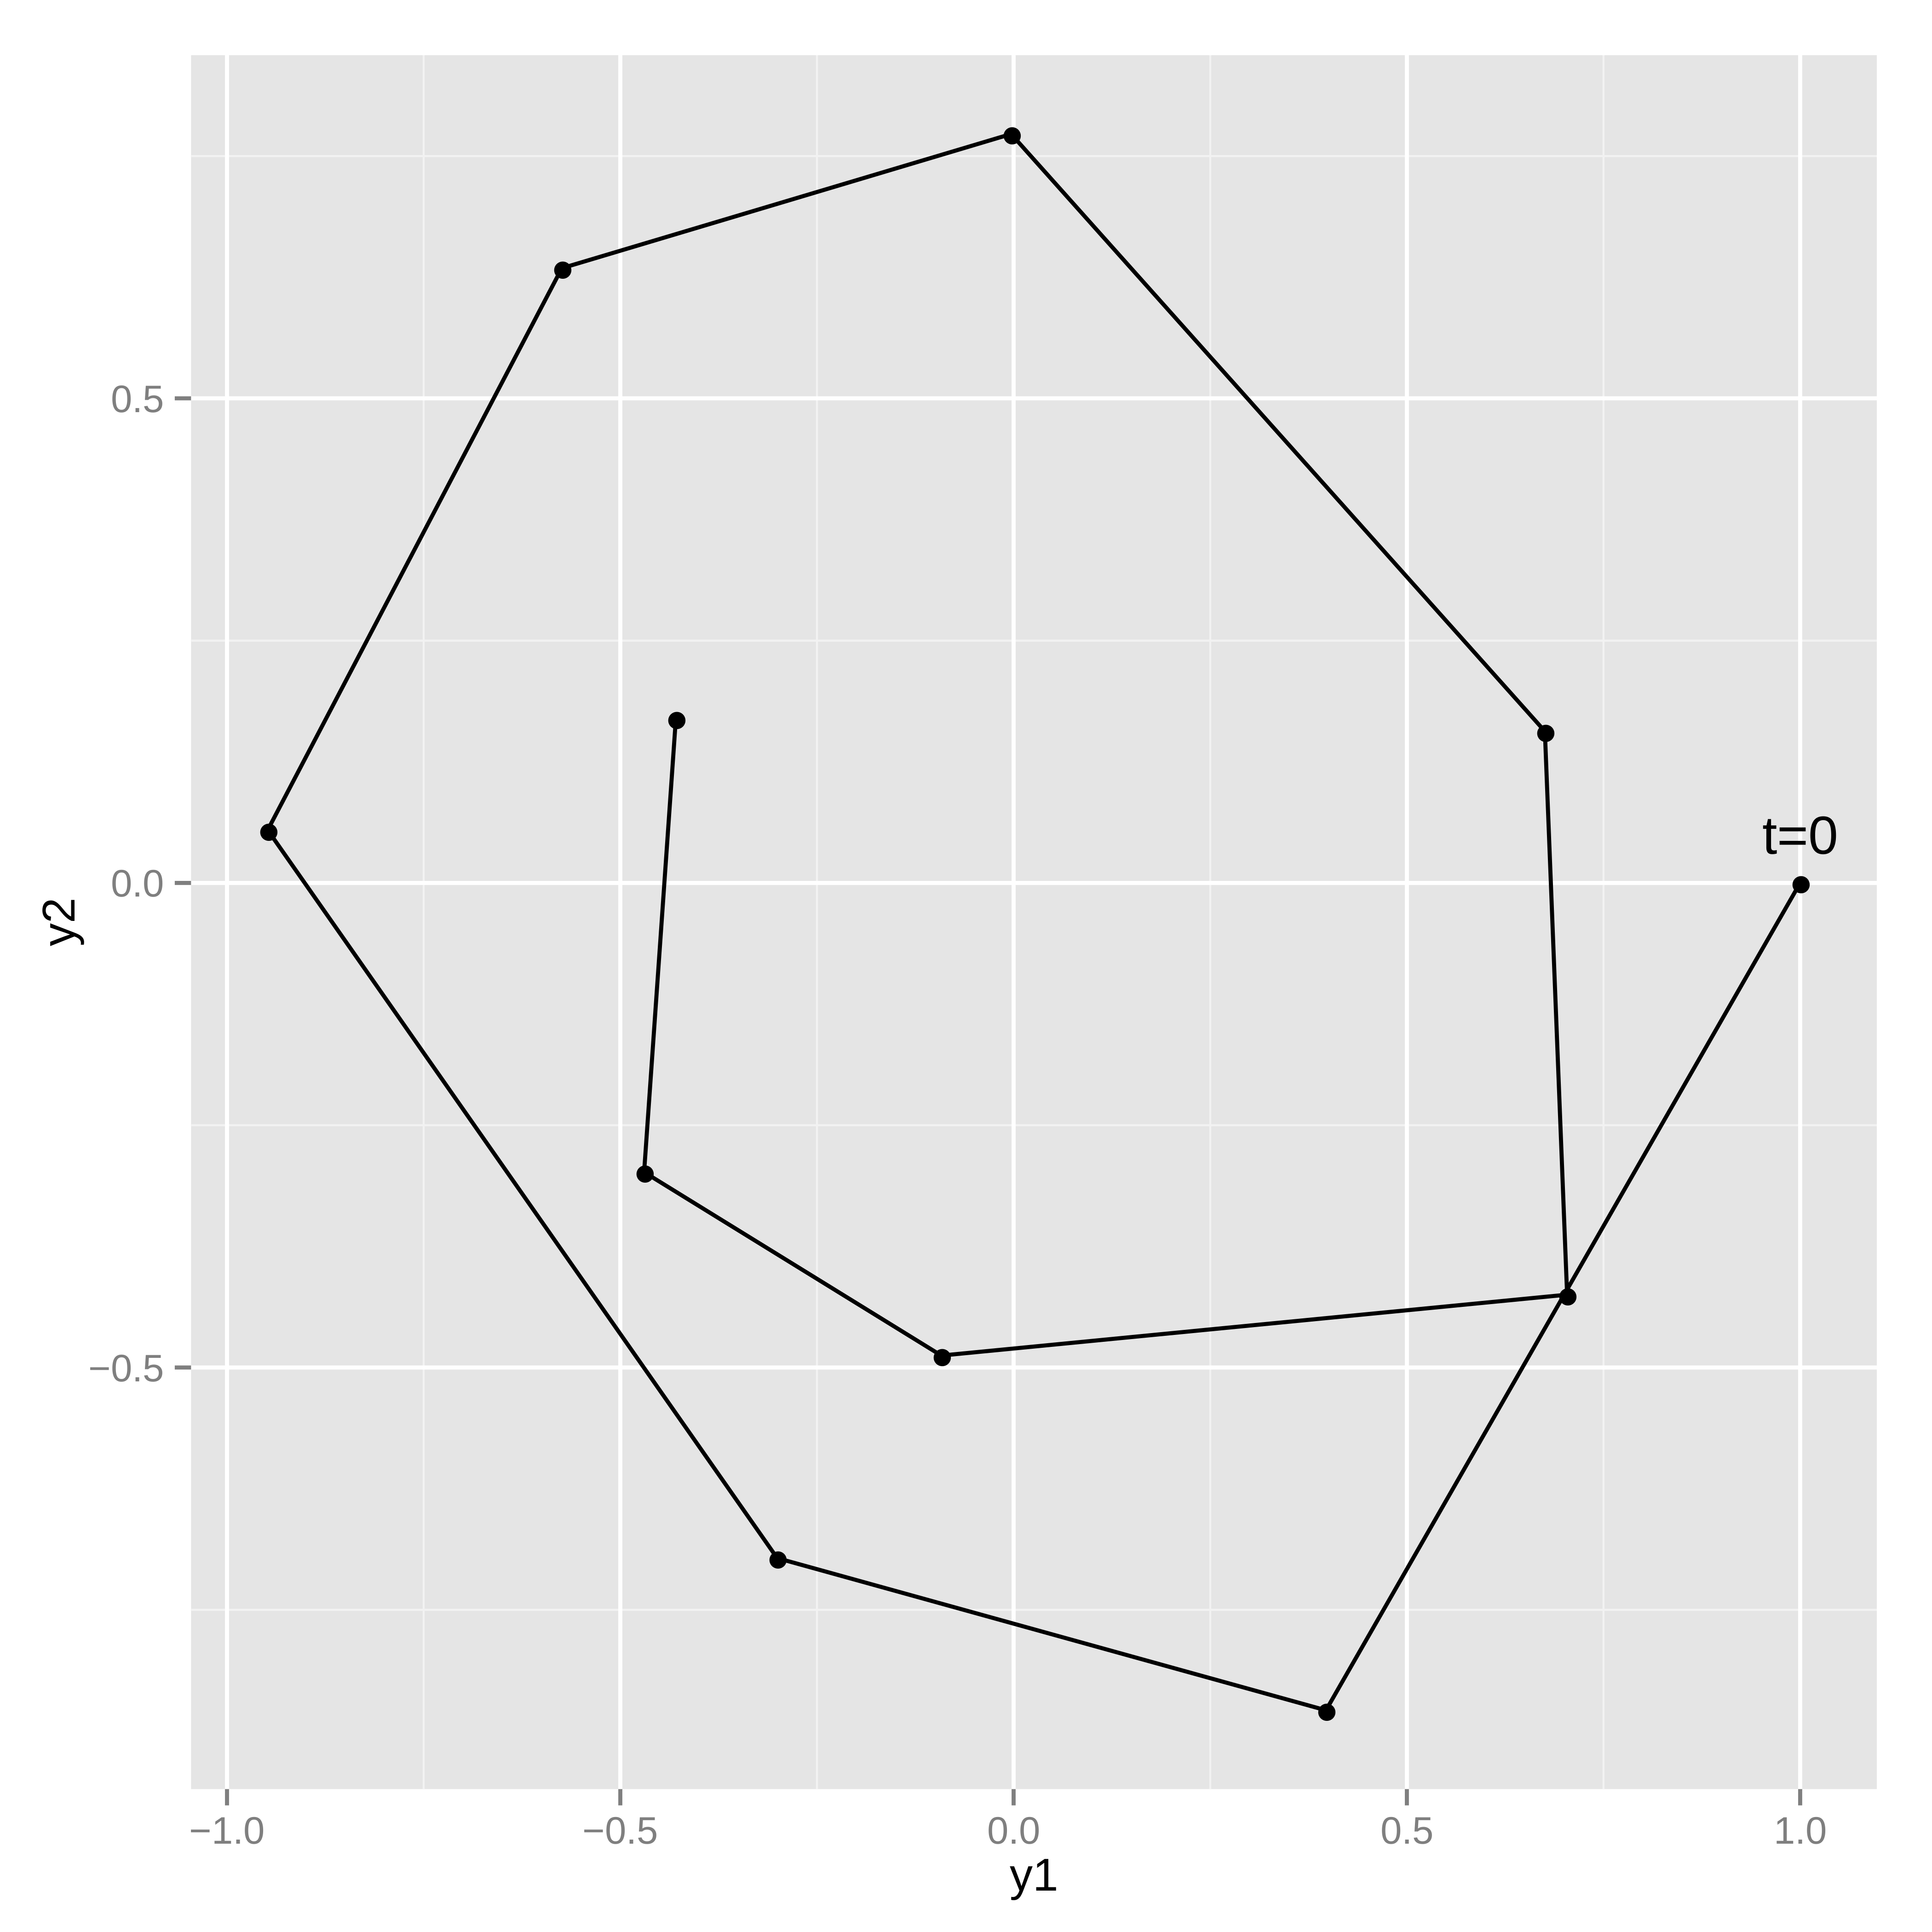
\includegraphics[width=0.7\linewidth]{./img/sho-ode-trajectory} 

}

\caption{Typical realization of harmonic oscillator trajectory.}\label{fig:unnamed-chunk-27}
\end{figure}

\hypertarget{estimating-system-parameters-and-initial-state}{%
\subsection*{Estimating system parameters and initial state}\label{estimating-system-parameters-and-initial-state}}
\addcontentsline{toc}{subsection}{Estimating system parameters and initial state}

These ten noisy observations of the state can be used to estimate the friction
parameter, \(\theta\), the initial conditions, \(y(t_0, \theta)\), and the scale of
the noise in the problem. The full Stan model is:

\newpage

\begin{Shaded}
\begin{Highlighting}[]
\KeywordTok{functions}\NormalTok{ \{}
  \DataTypeTok{vector}\NormalTok{ sho(}\DataTypeTok{real}\NormalTok{ t,}
             \DataTypeTok{vector}\NormalTok{ y,}
             \DataTypeTok{real}\NormalTok{ theta) \{}
    \DataTypeTok{vector}\NormalTok{[}\DecValTok{2}\NormalTok{] dydt;}
\NormalTok{    dydt[}\DecValTok{1}\NormalTok{] = y[}\DecValTok{2}\NormalTok{];}
\NormalTok{    dydt[}\DecValTok{2}\NormalTok{] = {-}y[}\DecValTok{1}\NormalTok{] {-} theta * y[}\DecValTok{2}\NormalTok{];}
    \ControlFlowTok{return}\NormalTok{ dydt;}
\NormalTok{  \}}
\NormalTok{\}}
\KeywordTok{data}\NormalTok{ \{}
  \DataTypeTok{int}\NormalTok{\textless{}}\KeywordTok{lower}\NormalTok{=}\DecValTok{1}\NormalTok{\textgreater{} T;}
  \DataTypeTok{array}\NormalTok{[T] }\DataTypeTok{vector}\NormalTok{[}\DecValTok{2}\NormalTok{] y;}
  \DataTypeTok{real}\NormalTok{ t0;}
  \DataTypeTok{array}\NormalTok{[T] }\DataTypeTok{real}\NormalTok{ ts;}
\NormalTok{\}}
\KeywordTok{parameters}\NormalTok{ \{}
  \DataTypeTok{vector}\NormalTok{[}\DecValTok{2}\NormalTok{] y0;}
  \DataTypeTok{vector}\NormalTok{\textless{}}\KeywordTok{lower}\NormalTok{=}\DecValTok{0}\NormalTok{\textgreater{}[}\DecValTok{2}\NormalTok{] sigma;}
  \DataTypeTok{real}\NormalTok{ theta;}
\NormalTok{\}}
\KeywordTok{model}\NormalTok{ \{}
  \DataTypeTok{array}\NormalTok{[T] }\DataTypeTok{vector}\NormalTok{[}\DecValTok{2}\NormalTok{] mu = ode\_rk45(sho, y0, t0, ts, theta);}
\NormalTok{  sigma \textasciitilde{} normal(}\DecValTok{0}\NormalTok{, }\FloatTok{2.5}\NormalTok{);}
\NormalTok{  theta \textasciitilde{} std\_normal();}
\NormalTok{  y0 \textasciitilde{} std\_normal();}
  \ControlFlowTok{for}\NormalTok{ (t }\ControlFlowTok{in} \DecValTok{1}\NormalTok{:T) \{}
\NormalTok{    y[t] \textasciitilde{} normal(mu[t], sigma);}
\NormalTok{  \}}
\NormalTok{\}}
\end{Highlighting}
\end{Shaded}

Because the solves are now a function of model parameters, the \texttt{ode\_rk45}
call is now made in the model block. There are half-normal priors on the
measurement error scales \texttt{sigma}, and standard normal priors on \texttt{theta} and the
initial state vector \texttt{y0}. The solutions to the ODE are assigned to \texttt{mu}, which
is used as the location for the normal observation model.

As with other regression models, it's easy to change the noise
model to something with heavier tails (e.g., Student-t distributed),
correlation in the state variables (e.g., with a multivariate
normal distribution), or both heavy tails and correlation in the state
variables (e.g., with a multivariate Student-t distribution).

\hypertarget{stiff-ode.section}{%
\section{Stiff ODEs}\label{stiff-ode.section}}

Stiffness is a numerical phenomena that causes some differential equation
solvers difficulty, notably the Runge-Kutta RK45 solver used in the examples
earlier. The phenomena is common in chemical reaction systems, which are often
characterized by having multiple vastly different time-scales. The stiffness of
a system can also vary between different parts of parameter space, and so a
typically non-stiff system may exhibit stiffness occasionally. These sorts of
difficulties can occur more frequently with loose priors or during warmup.

Stan provides a specialized solver for stiff ODEs
(\protect\hyperlink{ref-CohenHindmarsh:1996}{Cohen and Hindmarsh 1996}; \protect\hyperlink{ref-SerbanHindmarsh:2005}{Serban and Hindmarsh 2005}). An ODE system is
specified exactly the same way with a function of exactly the same
signature. The only difference is in the call to the solver the
\texttt{rk45} suffix is replaced with \texttt{bdf}, as in

\begin{Shaded}
\begin{Highlighting}[]
\NormalTok{ode\_bdf(sho, y0, t0, ts, theta);}
\end{Highlighting}
\end{Shaded}

Using the stiff (\texttt{bdf}) solver on a system that is not stiff
may be much slower than using the non-stiff (\texttt{rk45}) solver because
each step of the stiff solver takes more time to compute. On the other hand,
attempting to use the non-stiff solver for a stiff system will cause
the timestep to become very small, leading the non-stiff solver taking more
time overall even if each step is easier to compute than for the stiff solver.

If it is not known for sure that an ODE system is stiff, run the model with
both the \texttt{rk45} and \texttt{bdf} solvers and see which is faster. If the \texttt{rk45}
solver is faster, then the problem is probably non-stiff, and then it makes
sense to try the \texttt{adams} solver as well. The \texttt{adams} solver uses higher order
methods which can take larger timesteps than the \texttt{rk45} solver, though similar
to the \texttt{bdf} solver each of these steps is more expensive to compute.

\hypertarget{control-ode.section}{%
\section{Control parameters for ODE solving}\label{control-ode.section}}

For additional control of the solves, both the stiff and non-stiff
forward ODE solvers have function signatures that makes it possible to
specify the \texttt{relative\_tolerance}, \texttt{absolute\_tolerance}, and
\texttt{max\_num\_steps} parameters. These are the same as the regular
function names but with \texttt{\_tol} appended to the end. All three control
arguments must be supplied with this signature (there are no
defaults).

\begin{Shaded}
\begin{Highlighting}[]
\DataTypeTok{array}\NormalTok{[T] }\DataTypeTok{vector}\NormalTok{[}\DecValTok{2}\NormalTok{] y\_sim = ode\_bdf\_tol(sho, y0, t0, ts,}
\NormalTok{                                 relative\_tolerance,}
\NormalTok{                                 absolute\_tolerance,}
\NormalTok{                                 max\_num\_steps,}
\NormalTok{                                 theta);}
\end{Highlighting}
\end{Shaded}

\texttt{relative\_tolerance} and \texttt{absolute\_tolerance} control accuracy the solver tries to achieve, and
\texttt{max\_num\_steps} specifies the maximum number of steps the solver will
take between output time points before throwing an error.

The control parameters must be data variables -- they cannot be
parameters or expressions that depend on parameters, including local
variables in any block other than transformed data and generated
quantities. User-defined function arguments may be qualified as only
allowing data arguments using the \texttt{data} qualifier.

For the RK45 and Cash-Karp solvers, the default values for relative and absolute tolerance are
both \(10^{-6}\) and the maximum number of steps between outputs is
one million. For the BDF and Adams solvers, the relative and absolute
tolerances are \(10^{-10}\) and the maximum number of steps between outputs is
one hundred million.

\hypertarget{discontinuous-ode-system-function}{%
\subsection*{Discontinuous ODE system function}\label{discontinuous-ode-system-function}}
\addcontentsline{toc}{subsection}{Discontinuous ODE system function}

If there are discontinuities in the ODE system function, it is best
to integrate the ODE between the discontinuities, stopping the solver at each
one, and restarting it on the other side.

Nonetheless, the ODE solvers will attempt to integrate over discontinuities
they encounters in the state function. The accuracy of the solution near the
discontinuity may be problematic (requiring many small steps). An example of
such a discontinuity is a lag in a pharmacokinetic model, where a
concentration is zero for times \(0 < t < t'\) and then positive for \(t \geq t'\).
In this example example, we would use code in the system such as

\begin{Shaded}
\begin{Highlighting}[]
\ControlFlowTok{if}\NormalTok{ (t \textless{} t\_lag) \{}
  \ControlFlowTok{return}\NormalTok{ [}\DecValTok{0}\NormalTok{, }\DecValTok{0}\NormalTok{]\textquotesingle{};}
\NormalTok{\} }\ControlFlowTok{else}\NormalTok{ \{}
  \CommentTok{// ... return non{-}zero vector...}
\NormalTok{\}}
\end{Highlighting}
\end{Shaded}

In general it is better to integrate up to \texttt{t\_lag} in one solve and
then integrate from \texttt{t\_lag} onwards in another. Mathematically, the
discontinuity can make the problem ill-defined and the numerical integrator
may behave erratically around it.

If the location of the discontinuity cannot be controlled precisely, or there is
some other rapidly change in ODE behavior, it can be useful to tell the ODE
solver to produce output in the neighborhood. This can help the ODE solver avoid
indiscriminately stepping over an important feature of the solution.

\hypertarget{tolerance-1}{%
\subsection*{Tolerance}\label{tolerance-1}}
\addcontentsline{toc}{subsection}{Tolerance}

The relative tolerance RTOL and absolute tolerance ATOL control the accuracy of the
numerical solution. Specifically, when solving an ODE with unknowns
\(y=(y_1,\dots,y_n)^T\), at every step the
solver controls estimated local error \(e=(e_1,\dots,e_n)^T\) through its weighted root-mean-square norm
(Serban and Hindmarsh (\protect\hyperlink{ref-SerbanHindmarsh:2005}{2005}), Hairer, Nørsett, and Wanner (\protect\hyperlink{ref-hairer:1993}{1993}))

\[
\sqrt{\sum_{i=1}^n{\frac{1}{n}\frac{e_i^2}{(\text{RTOL}\times y_i + \text{ATOL})^2}}} < 1
\]
by reducing the stepsize when the inequality is not satisfied.

To understand the roles of the two tolerances it helps to assume \(y\) at
opposite scales in the above expression: on one hand the absolute
tolerance has little effect when \(y_i \gg 1\), on the other the
relative tolerance can
not affect the norm when \(y_i = 0\). Users are strongly encouraged to carefully choose
tolerance values according to the ODE and its application. One can follow
Brenan, Campbell, and Petzold (\protect\hyperlink{ref-Brenan:1996}{1995}) for a rule of thumb:
let \(m\) be the number of significant digits required for \(y\), set
\(\text{RTOL}=10^{-(m+1)}\), and set ATOL at
which \(y\) becomes insignificant. Note that the same weighted root-mean-square norm
is used to control nonlinear solver convergence in \texttt{bdf} and \texttt{adams} solvers, and the same
tolerances are used to control forward sensitivity calculation. See
Serban and Hindmarsh (\protect\hyperlink{ref-SerbanHindmarsh:2005}{2005}) for details.

\hypertarget{maximum-number-of-steps-1}{%
\subsection*{Maximum number of steps}\label{maximum-number-of-steps-1}}
\addcontentsline{toc}{subsection}{Maximum number of steps}

The maximum number of steps can be used to stop a runaway simulation.
This can arise in when MCMC moves to a part of parameter space very far from
where a differential equation would typically be solved. In particular this
can happen during warmup. With the non-stiff solver, this may happen when
the sampler moves to stiff regions of parameter space, which will requires small
step sizes.

\hypertarget{adjoint-ode.section}{%
\section{Adjoint ODE solver}\label{adjoint-ode.section}}

The adjoint ODE solver method differs mathematically from the forward
ODE solvers in the way gradients of the ODE solution are obtained. The
forward ODE approach augments the original ODE system with \(N\)
additional states for each parameter for which gradients are
needed. If there are \(M\) parameters for which sensitivities are
required, then the augmented ODE system has a total of \(N \cdot (M + 1)\) states. This can result in very large ODE systems through the
multiplicative scaling of the computational effort needed.

In contrast, the adjoint ODE solver integrates forward in time a
system of \(N\) equations to compute the ODE solution and then integrates
backwards in time another system of \(N\) equations to get the sensitivities.
Additionally, for \(M\) parameters there are \(M\) additional equations
to integrate during the backwards solve. Because of this the adjoint
sensitivity problem scales better in parameters than the forward
sensitivity problem. The adjoint solver in Stan uses CVODES (the same
as the \texttt{bdf} and \texttt{adams} forward sensitivity interfaces).

The solution computed in the forward integration is required during the
backward integration. CVODES uses a checkpointing scheme that saves the
forward solver state regularly. The number of steps between saving
checkpoints is configurable in the interface. These checkpoints are
then interpolated during the backward solve using one of two
interpolation schemes.

The solver type (either \texttt{bdf} or \texttt{adams}) can be individually set for
both the forward and backward solves.

The tolerances for each phase of the solve must be specified in the
interface. Note that the absolute tolerance for the forward and
backward ODE integration phase need to be set for each
ODE state separately. The harmonic oscillator example call from above
becomes:

\begin{Shaded}
\begin{Highlighting}[]
\DataTypeTok{array}\NormalTok{[T] }\DataTypeTok{vector}\NormalTok{[}\DecValTok{2}\NormalTok{] y\_sim}
\NormalTok{    = ode\_adjoint\_tol\_ctl(sho, y0, t0, ts,}
\NormalTok{                          relative\_tolerance/}\FloatTok{9.0}\NormalTok{,                }\CommentTok{// forward tolerance}
\NormalTok{                          rep\_vector(absolute\_tolerance/}\FloatTok{9.0}\NormalTok{, }\DecValTok{2}\NormalTok{), }\CommentTok{// forward tolerance}
\NormalTok{                          relative\_tolerance/}\FloatTok{3.0}\NormalTok{,                }\CommentTok{// backward tolerance}
\NormalTok{                          rep\_vector(absolute\_tolerance/}\FloatTok{3.0}\NormalTok{, }\DecValTok{2}\NormalTok{), }\CommentTok{// backward tolerance}
\NormalTok{                          relative\_tolerance,                    }\CommentTok{// quadrature tolerance}
\NormalTok{                          absolute\_tolerance,                    }\CommentTok{// quadrature tolerance}
\NormalTok{                          max\_num\_steps,}
                          \DecValTok{150}\NormalTok{,                                   }\CommentTok{// number of steps between checkpoints}
                          \DecValTok{1}\NormalTok{,                                     }\CommentTok{// interpolation polynomial: 1=Hermite, 2=polynomial}
                          \DecValTok{2}\NormalTok{,                                     }\CommentTok{// solver for forward phase: 1=Adams, 2=BDF }
                          \DecValTok{2}\NormalTok{,                                     }\CommentTok{// solver for backward phase: 1=Adams, 2=BDF }
\NormalTok{                          theta);}
\end{Highlighting}
\end{Shaded}

For a detailed information on each argument please see the
Stan function reference manual.

\hypertarget{solving-a-system-of-linear-odes-using-a-matrix-exponential}{%
\section{Solving a system of linear ODEs using a matrix exponential}\label{solving-a-system-of-linear-odes-using-a-matrix-exponential}}

Linear systems of ODEs can be solved using a matrix exponential. This can be
considerably faster than using one of the ODE solvers.

The solution to \(\frac{d}{dt} y = ay\) is \(y = y_0e^{at}\), where the constant
\(y_0\) is determined by boundary conditions. We can extend this solution
to the vector case:
\[
\frac{d}{dt}y = A \, y
\]
where \(y\) is now a vector of length \(n\) and \(A\) is an \(n\) by \(n\) matrix. The
solution is then given by:
\[
y = e^{tA} \, y_0
\]
where the matrix exponential is formally defined by the convergent power series:
\[
e^{tA} = \sum_{n=0}^{\infty} \dfrac{tA^n}{n!} = I + tA + \frac{t^2A^2}{2!} + \dotsb
\]

We can apply this technique to the simple harmonic oscillator example, by
setting
\[
y = \begin{bmatrix} y_1 \\ y_2 \end{bmatrix} \qquad
A = \begin{bmatrix} 0 & 1 \\ -1 & -\theta \end{bmatrix}
\]

The Stan model to simulate noisy observations using a matrix exponential function
is given below.

In general, computing a matrix exponential will be more efficient than using a numerical
solver. We can however only apply this technique to systems of linear ODEs.

\begin{Shaded}
\begin{Highlighting}[]
\KeywordTok{data}\NormalTok{ \{}
  \DataTypeTok{int}\NormalTok{\textless{}}\KeywordTok{lower}\NormalTok{=}\DecValTok{1}\NormalTok{\textgreater{} T;}
  \DataTypeTok{vector}\NormalTok{[}\DecValTok{2}\NormalTok{] y0;}
  \DataTypeTok{array}\NormalTok{[T] }\DataTypeTok{real}\NormalTok{ ts;}
  \DataTypeTok{array}\NormalTok{[}\DecValTok{1}\NormalTok{] }\DataTypeTok{real}\NormalTok{ theta;}
\NormalTok{\}}
\KeywordTok{model}\NormalTok{ \{}
\NormalTok{\}}
\KeywordTok{generated quantities}\NormalTok{ \{}
  \DataTypeTok{array}\NormalTok{[T] }\DataTypeTok{vector}\NormalTok{[}\DecValTok{2}\NormalTok{] y\_sim;}
  \DataTypeTok{matrix}\NormalTok{[}\DecValTok{2}\NormalTok{, }\DecValTok{2}\NormalTok{] A = [[ }\DecValTok{0}\NormalTok{,  }\DecValTok{1}\NormalTok{],}
\NormalTok{                    [{-}}\DecValTok{1}\NormalTok{, {-}theta[}\DecValTok{1}\NormalTok{]]]}
  \ControlFlowTok{for}\NormalTok{ (t }\ControlFlowTok{in} \DecValTok{1}\NormalTok{:T) \{}
\NormalTok{    y\_sim[t] = matrix\_exp((t {-} }\DecValTok{1}\NormalTok{) * A) * y0;}
\NormalTok{  \}}
  \CommentTok{// add measurement error}
  \ControlFlowTok{for}\NormalTok{ (t }\ControlFlowTok{in} \DecValTok{1}\NormalTok{:T) \{}
\NormalTok{    y\_sim[t, }\DecValTok{1}\NormalTok{] += normal\_rng(}\DecValTok{0}\NormalTok{, }\FloatTok{0.1}\NormalTok{);}
\NormalTok{    y\_sim[t, }\DecValTok{2}\NormalTok{] += normal\_rng(}\DecValTok{0}\NormalTok{, }\FloatTok{0.1}\NormalTok{);}
\NormalTok{  \}}
\NormalTok{\}}
\end{Highlighting}
\end{Shaded}

This Stan program simulates noisy measurements from a simple harmonic
oscillator. The system of linear differential equations is coded as a
matrix. The system parameters \texttt{theta} and initial state \texttt{y0} are read
in as data along observation times \texttt{ts}. The generated quantities
block is used to solve the ODE for the specified times and then add
random measurement error, producing observations \texttt{y\_sim}. Because the
ODEs are linear, we can use the \texttt{matrix\_exp} function to solve the
system.

\hypertarget{integrate-1d}{%
\chapter{Computing One Dimensional Integrals}\label{integrate-1d}}

Definite and indefinite one dimensional integrals can be performed in Stan
using the \href{https://mc-stan.org/docs/functions-reference/functions-1d-integrator.html}{\texttt{integrate\_1d} function}.

As an example, the normalizing constant of a left-truncated normal distribution is

\[
  \int_a^\infty \frac{1}{\sqrt{2 \pi \sigma^2}} e^{-\frac{1}{2}\frac{(x - \mu)^2}{\sigma^2}}
\]

To compute this integral in Stan, the integrand must first be defined as a Stan function
(see the Stan Reference Manual chapter on User-Defined Functions
for more information on coding user-defined functions).

\begin{Shaded}
\begin{Highlighting}[]
\DataTypeTok{real}\NormalTok{ normal\_density(}\DataTypeTok{real}\NormalTok{ x,             }\CommentTok{// Function argument}
                    \DataTypeTok{real}\NormalTok{ xc,            }\CommentTok{// Complement of function argument}
                                        \CommentTok{//  on the domain (defined later)}
                    \DataTypeTok{array}\NormalTok{[] }\DataTypeTok{real}\NormalTok{ theta, }\CommentTok{// parameters}
                    \DataTypeTok{array}\NormalTok{[] }\DataTypeTok{real}\NormalTok{ x\_r,   }\CommentTok{// data (real)}
                    \DataTypeTok{array}\NormalTok{[] }\DataTypeTok{int}\NormalTok{ x\_i) \{  }\CommentTok{// data (integer)}
  \DataTypeTok{real}\NormalTok{ mu = theta[}\DecValTok{1}\NormalTok{];}
  \DataTypeTok{real}\NormalTok{ sigma = theta[}\DecValTok{2}\NormalTok{];}

  \ControlFlowTok{return} \DecValTok{1}\NormalTok{ / (sqrt(}\DecValTok{2}\NormalTok{ * pi()) * sigma) * exp({-}}\FloatTok{0.5}\NormalTok{ * ((x {-} mu) / sigma)\^{}}\DecValTok{2}\NormalTok{);}
\NormalTok{\}}
\end{Highlighting}
\end{Shaded}

This function is expected to return the value of the integrand evaluated at point \texttt{x}. The
argument \texttt{xc} is used in definite integrals to avoid loss of precision near
the limits of integration and is set to NaN when either limit is infinite
(see the section on precision/loss in the chapter on
Higher-Order Functions
of the Stan Functions Reference for details on how to use this).
The argument \texttt{theta} is used to pass in arguments of the integral
that are a function of the parameters in our model. The arguments \texttt{x\_r}
and \texttt{x\_i} are used to pass in real and integer arguments of the integral that are
not a function of our parameters.

The function defining the integrand must have exactly the argument types and
return type of \texttt{normal\_density} above, though argument naming is not important.
Even if \texttt{x\_r} and \texttt{x\_i} are unused in the integrand, they must be
included in the function signature. This may require passing in zero-length arrays
for data or a zero-length vector for parameters if the integral does not involve
data or parameters.

\hypertarget{calling-the-integrator}{%
\section{Calling the integrator}\label{calling-the-integrator}}

Suppose that our model requires evaluating the lpdf of a left-truncated normal, but
the truncation limit is to be estimated as a parameter. Because the truncation
point is a parameter, we must include the normalization term of the truncated pdf when
computing our model's log density. Note this is just an example of how to use the
1D integrator. The more efficient way to perform the correct normalization in Stan
is described in the chapter on Truncated or Censored Data of this guide.

Such a model might look like (include the function defined at the beginning of this
chapter to make this code compile):

\begin{Shaded}
\begin{Highlighting}[]
\KeywordTok{data}\NormalTok{ \{}
  \DataTypeTok{int}\NormalTok{ N;}
  \DataTypeTok{array}\NormalTok{[N] }\DataTypeTok{real}\NormalTok{ y;}
\NormalTok{\}}

\KeywordTok{transformed data}\NormalTok{ \{}
  \DataTypeTok{array}\NormalTok{[}\DecValTok{0}\NormalTok{] }\DataTypeTok{real}\NormalTok{ x\_r;}
  \DataTypeTok{array}\NormalTok{[}\DecValTok{0}\NormalTok{] }\DataTypeTok{int}\NormalTok{ x\_i;}
\NormalTok{\}}

\KeywordTok{parameters}\NormalTok{ \{}
  \DataTypeTok{real}\NormalTok{ mu;}
  \DataTypeTok{real}\NormalTok{\textless{}}\KeywordTok{lower}\NormalTok{=}\FloatTok{0.0}\NormalTok{\textgreater{} sigma;}
  \DataTypeTok{real}\NormalTok{ left\_limit;}
\NormalTok{\}}

\KeywordTok{model}\NormalTok{ \{}
\NormalTok{  mu \textasciitilde{} normal(}\DecValTok{0}\NormalTok{, }\DecValTok{1}\NormalTok{);}
\NormalTok{  sigma \textasciitilde{} normal(}\DecValTok{0}\NormalTok{, }\DecValTok{1}\NormalTok{);}
\NormalTok{  left\_limit \textasciitilde{} normal(}\DecValTok{0}\NormalTok{, }\DecValTok{1}\NormalTok{);}
  \KeywordTok{target +=}\NormalTok{ normal\_lpdf(y | mu, sigma);}
  \KeywordTok{target +=}\NormalTok{ log(integrate\_1d(normal\_density,}
\NormalTok{                             left\_limit,}
\NormalTok{                             positive\_infinity(),}
\NormalTok{                             \{ mu, sigma \}, x\_r, x\_i));}
\NormalTok{\}}
\end{Highlighting}
\end{Shaded}

\hypertarget{limits-of-integration}{%
\subsection{Limits of integration}\label{limits-of-integration}}

The limits of integration can be finite or infinite. The infinite limits are
made available via the Stan calls \texttt{negative\_infinity()} and
\texttt{positive\_infinity()}.

If both limits are either \texttt{negative\_infinity()} or
\texttt{positive\_infinity()}, the integral and its gradients are set to zero.

\hypertarget{data-vs.-parameters}{%
\subsection{Data vs.~parameters}\label{data-vs.-parameters}}

The arguments for the real data \texttt{x\_r} and the integer data \texttt{x\_i}
must be expressions that only involve data or transformed data variables.
\texttt{theta}, on the other hand, can be a function of data, transformed data,
parameters, or transformed parameters.

The endpoints of integration can be data or parameters (and internally the
derivatives of the integral with respect to the endpoints are handled
with the Leibniz integral rule).

\hypertarget{integrator-convergence}{%
\section{Integrator convergence}\label{integrator-convergence}}

The integral is performed with the iterative 1D quadrature methods implemented
in the Boost library (\protect\hyperlink{ref-BoostQuadrature:2017}{Agrawal et al. 2017}). If the \(n\)th estimate of the
integral is denoted \(I_n\) and the \(n\)th estimate of the norm of the integral is
denoted \(|I|_n\), the iteration is terminated when

\[
  \frac{{|I_{n + 1} - I_n|}}{{|I|_{n + 1}}} < \text{relative tolerance}.
\]

The \texttt{relative\_tolerance} parameter can be optionally specified as the
last argument to \texttt{integrate\_1d}. By default, \texttt{integrate\_1d} follows the
Boost library recommendation of setting \texttt{relative\_tolerance} to the square
root of the machine epsilon of double precision floating point numbers
(about \texttt{1e-8}).

\hypertarget{zero-crossing}{%
\subsection{Zero-crossing integrals}\label{zero-crossing}}

Integrals on the (possibly infinite) interval \((a, b)\) that cross zero are
split into two integrals, one from \((a, 0)\) and one from \((0, b)\). This is
because the quadrature methods employed internally can have difficulty near
zero.

In this case, each integral is separately integrated to the given
\texttt{relative\_tolerance}.

\hypertarget{integral-precision}{%
\subsection{Avoiding precision loss near limits of integration in definite integrals}\label{integral-precision}}

If care is not taken, the quadrature can suffer from numerical loss of
precision near the endpoints of definite integrals.

For instance, in integrating the pdf of a beta distribution when the values of
\(\alpha\) and \(\beta\) are small, most of the probability mass is lumped near zero
and one.

The pdf of a beta distribution is proportional to

\[
p(x) \propto x^{\alpha - 1}(1 - x)^{\beta - 1}
\]

Normalizing this distribution requires computing the integral of \(p(x)\) from
zero to one. In Stan code, the integrand might look like:

\begin{Shaded}
\begin{Highlighting}[]
\DataTypeTok{real}\NormalTok{ beta(}\DataTypeTok{real}\NormalTok{ x, }\DataTypeTok{real}\NormalTok{ xc, }\DataTypeTok{array}\NormalTok{[] }\DataTypeTok{real}\NormalTok{ theta, }\DataTypeTok{array}\NormalTok{[] }\DataTypeTok{real}\NormalTok{ x\_r, }\DataTypeTok{array}\NormalTok{[] }\DataTypeTok{int}\NormalTok{ x\_i) \{}
  \DataTypeTok{real}\NormalTok{ alpha = theta[}\DecValTok{1}\NormalTok{];}
  \DataTypeTok{real}\NormalTok{ beta = theta[}\DecValTok{2}\NormalTok{];}

  \ControlFlowTok{return}\NormalTok{ x\^{}(alpha {-} }\FloatTok{1.0}\NormalTok{) * (}\FloatTok{1.0}\NormalTok{ {-} x)\^{}(beta {-} }\FloatTok{1.0}\NormalTok{);}
\NormalTok{\}}
\end{Highlighting}
\end{Shaded}

The issue is that there will be numerical breakdown in the precision of
\texttt{1.0\ -\ x} as \texttt{x} gets close to one. This is because of the limited
precision of double precision floating numbers. This integral will fail to
converge for values of \texttt{alpha} and \texttt{beta} much less than one.

This is where \texttt{xc} is useful. It is defined, for definite integrals, as a high
precision version of the distance from \texttt{x} to the nearest endpoint --- \texttt{a\ -\ x}
or \texttt{b\ -\ x} for a lower endpoint \texttt{a} and an upper endpoint \texttt{b}. To make use of
this for the beta integral, the integrand can be re-coded:

\begin{Shaded}
\begin{Highlighting}[]
\DataTypeTok{real}\NormalTok{ beta(}\DataTypeTok{real}\NormalTok{ x, }\DataTypeTok{real}\NormalTok{ xc, }\DataTypeTok{array}\NormalTok{[] }\DataTypeTok{real}\NormalTok{ theta, }\DataTypeTok{array}\NormalTok{[] }\DataTypeTok{real}\NormalTok{ x\_r, }\DataTypeTok{array}\NormalTok{[] }\DataTypeTok{int}\NormalTok{ x\_i) \{}
  \DataTypeTok{real}\NormalTok{ alpha = theta[}\DecValTok{1}\NormalTok{];}
  \DataTypeTok{real}\NormalTok{ beta = theta[}\DecValTok{2}\NormalTok{];}
  \DataTypeTok{real}\NormalTok{ v;}

  \ControlFlowTok{if}\NormalTok{(x \textgreater{} }\FloatTok{0.5}\NormalTok{) \{}
\NormalTok{    v = x\^{}(alpha {-} }\FloatTok{1.0}\NormalTok{) * xc\^{}(beta {-} }\FloatTok{1.0}\NormalTok{);}
\NormalTok{  \} }\ControlFlowTok{else}\NormalTok{ \{}
\NormalTok{    v = x\^{}(alpha {-} }\FloatTok{1.0}\NormalTok{) * (}\FloatTok{1.0}\NormalTok{ {-} x)\^{}(beta {-} }\FloatTok{1.0}\NormalTok{);}
\NormalTok{  \}}

  \ControlFlowTok{return}\NormalTok{ v;}
\NormalTok{\}}
\end{Highlighting}
\end{Shaded}

In this case, as we approach the upper limit of integration \(a = 1\), \texttt{xc} will
take on the value of \(a - x = 1 - x\). This version of the integrand will
converge for much smaller values of \texttt{alpha} and \texttt{beta} than otherwise possible.

Consider another example: let's say we have a log-normal distribution that is
both shifted away from zero by some amount \(\delta\), and truncated at some
value \(b\). If we were interested in calculating the expectation of a variable
\(X\) distributed in this way, we would need to calculate
\[
\int_a^b xf(x)\,dx = \int_{\delta}^b xf(x)\,dx
\]
in the numerator, where \(f(x)\) is the probability density function for the
shifted log-normal distribution. This probability density function can be
coded in Stan as:

\begin{Shaded}
\begin{Highlighting}[]
\DataTypeTok{real}\NormalTok{ shift\_lognormal\_pdf(}\DataTypeTok{real}\NormalTok{ x,}
                         \DataTypeTok{real}\NormalTok{ mu,}
                         \DataTypeTok{real}\NormalTok{ sigma,}
                         \DataTypeTok{real}\NormalTok{ delta) \{}
  \DataTypeTok{real}\NormalTok{ p;}

\NormalTok{  p = (}\FloatTok{1.0}\NormalTok{ / ((x {-} delta) * sigma * sqrt(}\DecValTok{2}\NormalTok{ * pi()))) *}
\NormalTok{    exp({-}}\DecValTok{1}\NormalTok{ * (log(x {-} delta) {-} mu)\^{}}\DecValTok{2}\NormalTok{ / (}\DecValTok{2}\NormalTok{ * sigma\^{}}\DecValTok{2}\NormalTok{));}

  \ControlFlowTok{return}\NormalTok{ p;}
\NormalTok{\}}
\end{Highlighting}
\end{Shaded}

Therefore, the function that we want to integrate is:

\begin{Shaded}
\begin{Highlighting}[]
\DataTypeTok{real}\NormalTok{ integrand(}\DataTypeTok{real}\NormalTok{ x,}
               \DataTypeTok{real}\NormalTok{ xc,}
               \DataTypeTok{array}\NormalTok{[] }\DataTypeTok{real}\NormalTok{ theta,}
               \DataTypeTok{array}\NormalTok{[] }\DataTypeTok{real}\NormalTok{ x\_r,}
               \DataTypeTok{array}\NormalTok{[] }\DataTypeTok{int}\NormalTok{ x\_i) \{}
  \DataTypeTok{real}\NormalTok{ numerator;}
  \DataTypeTok{real}\NormalTok{ p;}

  \DataTypeTok{real}\NormalTok{ mu = theta[}\DecValTok{1}\NormalTok{];}
  \DataTypeTok{real}\NormalTok{ sigma = theta[}\DecValTok{2}\NormalTok{];}
  \DataTypeTok{real}\NormalTok{ delta = theta[}\DecValTok{3}\NormalTok{];}
  \DataTypeTok{real}\NormalTok{ b = theta[}\DecValTok{4}\NormalTok{];}

\NormalTok{  p = shift\_lognormal\_pdf(x, mu, sigma, delta);}

\NormalTok{  numerator = x * p;}

  \ControlFlowTok{return}\NormalTok{ numerator;}
\NormalTok{\}}
\end{Highlighting}
\end{Shaded}

What happens here is that, given that the log-normal distribution is shifted by
\(\delta\), when we then try to integrate the numerator, our \texttt{x} starts at
values just above \texttt{delta}. This, in turn, causes the \texttt{x\ -\ delta} term to be
near zero, leading to a breakdown.

We can use \texttt{xc}, and define the \texttt{integrand} as:

\begin{Shaded}
\begin{Highlighting}[]
\DataTypeTok{real}\NormalTok{ integrand(}\DataTypeTok{real}\NormalTok{ x,}
               \DataTypeTok{real}\NormalTok{ xc,}
               \DataTypeTok{array}\NormalTok{[] }\DataTypeTok{real}\NormalTok{ theta,}
               \DataTypeTok{array}\NormalTok{[] }\DataTypeTok{real}\NormalTok{ x\_r,}
               \DataTypeTok{array}\NormalTok{[] }\DataTypeTok{int}\NormalTok{ x\_i) \{}
  \DataTypeTok{real}\NormalTok{ numerator;}
  \DataTypeTok{real}\NormalTok{ p;}

  \DataTypeTok{real}\NormalTok{ mu = theta[}\DecValTok{1}\NormalTok{];}
  \DataTypeTok{real}\NormalTok{ sigma = theta[}\DecValTok{2}\NormalTok{];}
  \DataTypeTok{real}\NormalTok{ delta = theta[}\DecValTok{3}\NormalTok{];}
  \DataTypeTok{real}\NormalTok{ b = theta[}\DecValTok{4}\NormalTok{];}

  \ControlFlowTok{if}\NormalTok{ (x \textless{} delta + }\DecValTok{1}\NormalTok{) \{}
\NormalTok{    p = shift\_lognormal\_pdf(xc, mu, sigma, delta);}
\NormalTok{  \} }\ControlFlowTok{else}\NormalTok{ \{}
\NormalTok{    p = shift\_lognormal\_pdf(x, mu, sigma, delta);}
\NormalTok{  \}}

\NormalTok{  numerator = x * p;}

  \ControlFlowTok{return}\NormalTok{ numerator;}
\NormalTok{\}}
\end{Highlighting}
\end{Shaded}

Why does this work? When our values of \texttt{x} are less than \texttt{delta\ +\ 1} (so, when
they're near \texttt{delta}, given that our lower bound of integration is equal to
\(\delta\)), we pass \texttt{xc} as an argument to our \texttt{shift\_lognormal\_pdf} function.
This way, instead of dealing with \texttt{x\ -\ delta} in \texttt{shift\_lognormal\_pdf}, we are
working with \texttt{xc\ -\ delta} which is equal to \texttt{delta\ -\ x\ -\ delta}, as \texttt{delta} is
the lower endpoint in that case. The \texttt{delta} terms cancel out, and we are left
with a high-precision version of \texttt{x}. We don't encounter the same problem at
the upper limit \(b\) so we don't adjust the code for that case.

Note, \texttt{xc} is only used for definite integrals. If either the left endpoint
is at negative infinity or the right endpoint is at positive infinity, \texttt{xc}
will be NaN.

For zero-crossing definite integrals (see section \protect\hyperlink{zero-crossing}{Zero Crossing}) the
integrals are broken into two pieces (\((a, 0)\) and \((0, b)\) for endpoints
\(a < 0\) and \(b > 0\)) and \texttt{xc} is a high precision version of the distance
to the limits of each of the two integrals separately. This means \texttt{xc} will
be a high precision version of \texttt{a\ -\ x}, \texttt{x}, or \texttt{b\ -\ x},
depending on the value of x and the endpoints.

\hypertarget{complex-numbers}{%
\chapter{Complex Numbers}\label{complex-numbers}}

Stan supports complex scalars, matrices, and vectors as well as
real-based ones.

\hypertarget{working-with-complex-numbers}{%
\section{Working with complex numbers}\label{working-with-complex-numbers}}

This section describes the complex scalar type, including how to build
complex numbers, assign them, and use them in arrays and functions.

\hypertarget{constructing-and-accessing-complex-numbers}{%
\subsection{Constructing and accessing complex numbers}\label{constructing-and-accessing-complex-numbers}}

Complex numbers can be constructed using imaginary literals. For example,

\begin{Shaded}
\begin{Highlighting}[]
\DataTypeTok{complex}\NormalTok{ z = {-}}\FloatTok{1.1}\NormalTok{ + }\FloatTok{2.3i}\NormalTok{;}
\end{Highlighting}
\end{Shaded}

produces the complex number \(-1.1 + 2.3i\). This only works if the
real and imaginary components are literal numerals. To construct a
complex number out of arbitrary real variables, the \texttt{to\_complex()}
function may be used. For example, the following code will work if
\texttt{x} and \texttt{y} are parameters, transformed data, or local variables in a
function or model block.

\begin{Shaded}
\begin{Highlighting}[]
\DataTypeTok{real}\NormalTok{ x = }\CommentTok{// ...}
\DataTypeTok{real}\NormalTok{ y = }\CommentTok{// ...}
\DataTypeTok{complex}\NormalTok{ z = to\_complex(x, y);}
\end{Highlighting}
\end{Shaded}

The real and imaginary parts of the complex number can be accessed
with getters as follows.

\begin{Shaded}
\begin{Highlighting}[]
\DataTypeTok{real}\NormalTok{ x = get\_real(z);  }\CommentTok{// x = {-}1.1}
\DataTypeTok{real}\NormalTok{ y = get\_imag(z);  }\CommentTok{// y = 2.3}
\end{Highlighting}
\end{Shaded}

Complex numbers can be compared using equality (or inequality), but
not with greater than or less than operators. For example, after
running the code above, the following code snippet will print
``hello''.

\begin{Shaded}
\begin{Highlighting}[]
\DataTypeTok{complex}\NormalTok{ a = }\FloatTok{3.2}\NormalTok{ + }\FloatTok{2i}\NormalTok{;}
\DataTypeTok{complex}\NormalTok{ b = to\_complex(}\FloatTok{3.2}\NormalTok{, }\DecValTok{2}\NormalTok{);}
\ControlFlowTok{if}\NormalTok{ (a == b) }\KeywordTok{print}\NormalTok{(}\StringTok{"hello"}\NormalTok{);}
\end{Highlighting}
\end{Shaded}

\hypertarget{complex-assignment-and-promotion}{%
\subsection{Complex assignment and promotion}\label{complex-assignment-and-promotion}}

Integer- or real-valued expressions may be assigned to complex
numbers, with the corresponding imaginary component set to zero.

\begin{Shaded}
\begin{Highlighting}[]
\DataTypeTok{complex}\NormalTok{ z1 = }\DecValTok{3}\NormalTok{;  }\CommentTok{// int promoted to 3 + 0i}
\DataTypeTok{complex}\NormalTok{ z2 = }\FloatTok{3.2}\NormalTok{;  }\CommentTok{// real promoted to 3.2 + 0.i}
\end{Highlighting}
\end{Shaded}

\hypertarget{complex-arrays}{%
\subsection{Complex arrays}\label{complex-arrays}}

Arrays of complex numbers work as usual and allow the usual
curly bracket constructors.

\begin{Shaded}
\begin{Highlighting}[]
\DataTypeTok{complex}\NormalTok{ z1;  }\DataTypeTok{complex}\NormalTok{ z2;  }\DataTypeTok{complex}\NormalTok{ z3;}
\CommentTok{// ...}
\DataTypeTok{array}\NormalTok{[}\DecValTok{3}\NormalTok{] }\DataTypeTok{complex}\NormalTok{ zs = \{ z1, z2, z3 \};}
\ControlFlowTok{for}\NormalTok{ (z }\ControlFlowTok{in}\NormalTok{ zs) \{}
  \KeywordTok{print}\NormalTok{(z);}
\NormalTok{\}}
\end{Highlighting}
\end{Shaded}

Complex arrays allow assignment into their elements, with integer or
real assigned values being promoted to complex.

\hypertarget{complex-functions}{%
\subsection{Complex functions}\label{complex-functions}}

All of the standard complex functions are available, including
natural logarithm \texttt{log(z)}, natural exponentiation \texttt{exp(z)}, and
powers \texttt{pow(z1,\ z2)}, as well as all of the trig and hyperbolic
trigonometric functions and their inverse, such as \texttt{sin(z)},
\texttt{acos(z)}, \texttt{tanh(z)} and \texttt{asinh(z)}.

Promotion also works for complex-valued function arguments, which may
be passed integer or real values, which will be promoted before the
function is evaluated. For example, the following user-defined
complex function will accept integer, real, or complex arguments.

\begin{Shaded}
\begin{Highlighting}[]
\DataTypeTok{complex}\NormalTok{ times\_i(}\DataTypeTok{complex}\NormalTok{ z) \{}
  \DataTypeTok{complex}\NormalTok{ i = to\_complex(}\DecValTok{0}\NormalTok{, }\DecValTok{1}\NormalTok{);}
  \ControlFlowTok{return}\NormalTok{ i * z;}
\NormalTok{\}}
\end{Highlighting}
\end{Shaded}

For instance, \texttt{times\_i(1)} evaluates to the imaginary base \(i\), as
does \texttt{times\_i(1.0)}.

\hypertarget{complex-random-variables}{%
\section{Complex random variables}\label{complex-random-variables}}

The simplest way to model a distribution over a complex random number
\(z = x = yi\) is to consider its real part \(x\) and imaginary part \(y\)
to have a bivariate normal distribution. For example, a complex prior
can be expressed as follows.

\begin{Shaded}
\begin{Highlighting}[]
\DataTypeTok{complex}\NormalTok{ z;}
\DataTypeTok{vector}\NormalTok{[}\DecValTok{2}\NormalTok{] mu;}
\NormalTok{cholesky\_cov[}\DecValTok{2}\NormalTok{] L\_Sigma;}
\CommentTok{// ...}
\NormalTok{[get\_real(z), get\_imag(z)]\textquotesingle{} \textasciitilde{} multi\_normal\_cholesky(mu, L\_Sigma);}
\end{Highlighting}
\end{Shaded}

For example, if \texttt{z} is data, this can be used to estimate \texttt{mu} and the
covariance Cholesky factor \texttt{L\_Sigma}. Alternatively, if \texttt{z} is
a parameter, \texttt{mu} and \texttt{L\_Sigma} may constants defining a prior or
further parameters defining a hierarchical model.

\hypertarget{complex-matrices-and-vectors}{%
\section{Complex matrices and vectors}\label{complex-matrices-and-vectors}}

Stan supports complex matrices, vectors, and row vectors. Variables
of these types are declared with sizes in the same way as their
real-based counterparts.

\begin{Shaded}
\begin{Highlighting}[]
\DataTypeTok{complex\_vector}\NormalTok{[}\DecValTok{3}\NormalTok{] v;}
\DataTypeTok{complex\_row\_vector}\NormalTok{[}\DecValTok{2}\NormalTok{] rv;}
\DataTypeTok{complex\_matrix}\NormalTok{[}\DecValTok{3}\NormalTok{, }\DecValTok{2}\NormalTok{] m;}
\end{Highlighting}
\end{Shaded}

We can construct vectors and matrices using brackets in the same way
as for real-valued vectors and matrices. For example, given the
declaration of \texttt{rv} above, we could assign it to a constructed row
vector.

\begin{Shaded}
\begin{Highlighting}[]
\NormalTok{rv =  [}\DecValTok{2}\NormalTok{ + }\FloatTok{3i}\NormalTok{, }\FloatTok{1.9}\NormalTok{ {-} }\FloatTok{2.3i}\NormalTok{];}
\end{Highlighting}
\end{Shaded}

Complex matrices and vectors support all of the standard arithetmic
operations including negation, addition, subtraction, and
multiplication (division involves a solve, and isn't a simple
arithmetic operation for matrices). They also support transposition.

Furthermore, it is possible to convert back and forth between arrays
and matrices using the \texttt{to\_array} functions.

\hypertarget{complex-linear-regression}{%
\section{Complex linear regression}\label{complex-linear-regression}}

Complex valued linear regression with complex predictors and
regression coefficients looks just like standard regression. For
example, if we take \texttt{x} to be predictors, \texttt{y} to be an array of
outcomes. For example, consider the following complete Stan program
for an intercept and slope.

\begin{Shaded}
\begin{Highlighting}[]
\KeywordTok{data}\NormalTok{ \{}
  \DataTypeTok{int}\NormalTok{\textless{}}\KeywordTok{lower}\NormalTok{=}\DecValTok{0}\NormalTok{\textgreater{} N;}
  \DataTypeTok{complex\_vector}\NormalTok{[N] x;}
  \DataTypeTok{complex\_vector}\NormalTok{[N] y;}
\NormalTok{\}}
\KeywordTok{parameters}\NormalTok{ \{}
  \DataTypeTok{complex}\NormalTok{ alpha;}
  \DataTypeTok{complex}\NormalTok{ beta;}
\NormalTok{\}}
\KeywordTok{model}\NormalTok{ \{}
  \DataTypeTok{complex\_vector}\NormalTok{[N] eps = y {-} (alpha + beta * x);}
\NormalTok{  eps \textasciitilde{}  }\CommentTok{// ...error distribution...}
\NormalTok{\}}
\end{Highlighting}
\end{Shaded}

The question remains of how to fill in the error distribution and
there are several alternatives. We consider only two simple
alternatives, and do not consider penalizing the absolute value of the
error.

\hypertarget{independent-real-and-imaginary-error}{%
\subsection{Independent real and imaginary error}\label{independent-real-and-imaginary-error}}

The simplest approach to error in complex regression is to give the
real and imaginary parts of \texttt{eps\_n} independent
independent normal distributions, as follows.

\begin{Shaded}
\begin{Highlighting}[]
\KeywordTok{parameters}\NormalTok{ \{}
  \CommentTok{// ...}
  \DataTypeTok{vector}\NormalTok{[}\DecValTok{2}\NormalTok{] sigma;}
\NormalTok{\}}
\CommentTok{// ...}
\KeywordTok{model}\NormalTok{ \{}
  \CommentTok{// ...}
\NormalTok{  get\_real(eps) \textasciitilde{} normal(}\DecValTok{0}\NormalTok{, sigma[}\DecValTok{1}\NormalTok{]);}
\NormalTok{  get\_imag(eps) \textasciitilde{} normal(}\DecValTok{0}\NormalTok{, sigma[}\DecValTok{2}\NormalTok{]);}
\NormalTok{  sigma \textasciitilde{} }\CommentTok{//...hyperprior...}
\NormalTok{\}}
\end{Highlighting}
\end{Shaded}

A new error scale vector \texttt{sigma} is introduced, and it should itself
get a prior based on the expected scale of error for the problem.

\hypertarget{dependent-complex-error}{%
\subsection{Dependent complex error}\label{dependent-complex-error}}

The next simplest approach is to treat the real and imaginary parts of
the complex number as having a multivariate normal prior. This can be
done by adding a parameter for correlation to the above, or just
working with a multivariate covariance matrix, as we do here.

\begin{Shaded}
\begin{Highlighting}[]
\KeywordTok{parameters}\NormalTok{ \{}
  \DataTypeTok{cholesky\_factor\_corr}\NormalTok{[}\DecValTok{2}\NormalTok{] L\_Omega;  }\CommentTok{// correlation matrix}
  \DataTypeTok{vector}\NormalTok{[}\DecValTok{2}\NormalTok{] sigma;                  }\CommentTok{// real, imag error scales}
  \CommentTok{// ...}
\NormalTok{\}}
\CommentTok{// ...}
\KeywordTok{model}\NormalTok{ \{}
  \DataTypeTok{array}\NormalTok{[N] }\DataTypeTok{vector}\NormalTok{[}\DecValTok{2}\NormalTok{] eps\_arr;}
  \ControlFlowTok{for}\NormalTok{ (n }\ControlFlowTok{in} \DecValTok{1}\NormalTok{:N) \{}
\NormalTok{    eps\_arr[n] = \{ to\_real(eps[n]), to\_imag(eps[n]) \};}
\NormalTok{  \}}
\NormalTok{  eps\_arr \textasciitilde{} multi\_normal\_cholesky([}\DecValTok{0}\NormalTok{, }\DecValTok{0}\NormalTok{]\textquotesingle{},}
\NormalTok{                                  diag\_pre\_multiply(sigma, L\_Omega));}
\NormalTok{  L\_Omega \textasciitilde{} lkj\_cholesky(}\DecValTok{4}\NormalTok{);  }\CommentTok{// shrink toward diagonal correlation}
\NormalTok{  sigma \textasciitilde{} }\CommentTok{// ... hyperprior ...}
\NormalTok{\}}
\end{Highlighting}
\end{Shaded}

Here, the real and imaginary components of the error get a joint
distribution with correlation and independent scales. The error gets
a multivariate normal distribution with zero mean and a Cholesky
factor representation of covariance, consisting of a scale vector
\texttt{sigma} and a Cholesky factor or a correlation matrix, \texttt{L\_Omega}. The
prior on the correlations is concentrated loosely around diagonal
covariance, and the prior on the scales is left open. In order to
vectorize the call to \texttt{multi\_normal\_cholesky}, the vector of complex
numbers needs to be converted to an array of size 2 vectors.

\hypertarget{dae-solver.chapter}{%
\chapter{Differential-Algebraic Equations}\label{dae-solver.chapter}}

Stan support solving systems of differential-algebraic equations
(DAEs) of index 1 (\protect\hyperlink{ref-serban_user:2021}{Serban et al. 2021}). The solver adaptively
refines the solutions in order to satisfy given tolerances.

One can think a differential-algebraic system of equations
as ODEs with additional algebraic constraits applied to some
of the variables. In such a system, the variable derivatives may not be
expressed explicitly with a right-hand-side as in ODEs, but implicitly
constrained.

Similar to ODE solvers, the DAE
solvers must not only provide the solution to the DAE itself, but also
the gradient of the DAE solution with respect to parameters (the
sensitivities). Stan's DAE solver uses
the \emph{forward sensitivity} calculation to expand the base DAE system
with additional DAE equations for the gradients of the solution.
For each parameter, an additional full set of \(N\)
sensitivity states are added meaning that the full DAE solved has
\[N \, + N \cdot M\] states.

Two interfaces are provided for the forward sensitivity solver: one
with default tolerances and default max number of steps, and one
that allows these controls to be modified. Choosing tolerances is
important for making any of the solvers work well -- the defaults
will not work everywhere. The tolerances should be chosen primarily
with consideration to the scales of the solutions, the accuracy
needed for the solutions, and how the solutions are used in the
model. The same principles in the \protect\hyperlink{control-ode.section}{control parameters
section} apply here.

Internally Stan's DAE solver uses a variable-step, variable-order,
backward-differentiation formula implementation
(\protect\hyperlink{ref-CohenHindmarsh:1996}{Cohen and Hindmarsh 1996}; \protect\hyperlink{ref-SerbanHindmarsh:2005}{Serban and Hindmarsh 2005}).

\hypertarget{notation-1}{%
\section{Notation}\label{notation-1}}

A DAE is defined by a set of expressions for the \emph{residuals} of differential equations and algebraic equations
\(r(y', y, t, \theta)\), and \emph{consistent} initial conditions
\(y(t_0, \theta) = y_0, y'(t_0, \theta)=y'_0\). The DAE is define by
residual function as \(r(y', y, t, \theta)=0\).
The \(\theta\) dependence is included in the notation to highlight that
the solution \(y(t)\) is
a function of any parameters used in the computation.

\hypertarget{example-chemical-kinetics}{%
\section{Example: chemical kinetics}\label{example-chemical-kinetics}}

As an example of a system of DAEs, consider following chemical
kinetics problem(\protect\hyperlink{ref-robertson_solution:1966}{Robertson 1966}). The nondimensionalized DAE consists of two differential equations
and one algebraic constraint. The differential equations describe the
reactions from reactants \(y_1\) and \(y_2\) to the product \(y_3\), and the
algebraic equation describes the mass conservation.
(\protect\hyperlink{ref-serban_example:2021}{Serban and Hindmarsh 2021}).

\[
\frac{dy_1}{dt} + \alpha y_1 - \beta y_2 y_3 = 0
\frac{dy_2}{dt} - \alpha y_1 + \beta y_2 y_3 + \gamma y_2^2 = 0
y_1 + y_2 + y_3 - 1.0 = 0
\]

The state equations implicitly defines the state \((y_1(t), y_2(t), y_3(t))\) at future times
as a function of an initial state and the system parameters, in this
example the reaction rate coefficients \((\alpha, \beta, \gamma)\).

Unlike solving ODEs, solving DAEs requires a \emph{consistent} initial
condition. That is, one must specify both \(y(t_0)\)
and \(y'(t_0)\) so that residual function becomes zero at initial time \(t_0\)
\[
r(y'(t_0), y(t_0), t_0) = 0
\]

\hypertarget{index-of-daes}{%
\section{Index of DAEs}\label{index-of-daes}}

The index along a DAE solution \(y(t)\) is the minimum number of
differentiations of some of the components of the system required to
solve for \(y'\) uniquely in terms of \(y\) and \(t\), so that the DAE is
converted into an ODE for \(y\). Thus an ODE system is of index 0. The
above chemical kinetics DAE is of index 1, as we can perform
differentiation of the third equation followed by introducing the
first two equations in order to obtain the ODE for \(y_3\).

Most DAE solvers, including the one in Stan, support only index-1
DAEs. For a high index DAE problem the user must first convert it to a
lower index system. This often can be done by carrying out
differentiations analytically (\protect\hyperlink{ref-ascher_computer:1998}{Ascher and Petzold 1998}).

\hypertarget{coding-the-dae-system-function}{%
\section{Coding the DAE system function}\label{coding-the-dae-system-function}}

The first step in coding an DAE system in Stan is defining the DAE residual
function. The system functions require a specific signature so that the solvers
know how to use them properly.

The first argument to the residual function is time, passed as a \texttt{real};
the second argument to the residual function is the system state \(y\),
passed as a \texttt{vector}, the third argument to the residual function is
the state derivative \(y'\), also passed as a \texttt{vector}. The residual
function's return value is a \texttt{vector} of the same size as state and
stae derivatives. Additional arguments
can be included in the residual function to pass other information
into the solve (these will be passed through the function that starts the DAE
solution). These argument can be parameters (in our example, the
reaction rate coefficient \(\alpha\), \(\beta\), and \(\gamma\)), data, or any quantities that are needed to define the
DAE.

The above reaction be coded using the following function
in Stan (see the \protect\hyperlink{functions-programming.chapter}{user-defined functions chapter} for
more information on coding user-defined functions).

\begin{Shaded}
\begin{Highlighting}[]
 \DataTypeTok{vector}\NormalTok{ chem(}\DataTypeTok{real}\NormalTok{ t, }\DataTypeTok{vector}\NormalTok{ yy, }\DataTypeTok{vector}\NormalTok{ yp,}
                 \DataTypeTok{real}\NormalTok{ alpha, }\DataTypeTok{real}\NormalTok{ beta, }\DataTypeTok{real}\NormalTok{ gamma) \{}
    \DataTypeTok{vector}\NormalTok{[}\DecValTok{3}\NormalTok{] res;}
\NormalTok{    res[}\DecValTok{1}\NormalTok{] = yp[}\DecValTok{1}\NormalTok{] + alpha * yy[}\DecValTok{1}\NormalTok{] {-} beta * yy[}\DecValTok{2}\NormalTok{] * yy[}\DecValTok{3}\NormalTok{];}
\NormalTok{    res[}\DecValTok{2}\NormalTok{] = yp[}\DecValTok{2}\NormalTok{] {-} alpha * yy[}\DecValTok{1}\NormalTok{] + beta * yy[}\DecValTok{2}\NormalTok{] * yy[}\DecValTok{3}\NormalTok{] + gamma * yy[}\DecValTok{2}\NormalTok{] * yy[}\DecValTok{2}\NormalTok{];}
\NormalTok{    res[}\DecValTok{3}\NormalTok{] = yy[}\DecValTok{1}\NormalTok{] + yy[}\DecValTok{2}\NormalTok{] + yy[}\DecValTok{3}\NormalTok{] {-} }\FloatTok{1.0}\NormalTok{;}
    \ControlFlowTok{return}\NormalTok{ res;}
\NormalTok{  \}}
\NormalTok{\}}
\end{Highlighting}
\end{Shaded}

The function takes in a time \texttt{t} (a \texttt{real}), the system state
\texttt{yy} (a \texttt{vector}), state derivative \texttt{yp} (a \texttt{vector}), as well as parameter
\texttt{alpha} (a \texttt{real}), \texttt{beta} (a \texttt{real}), and \texttt{gamma} (a \texttt{real}). The function returns a
\texttt{vector} of the residuals at time \texttt{t}. The DAE coded here does not
explicitly depend on \texttt{t}, however one still needs to specify \texttt{t} as
an argument.

\hypertarget{strict-signature-2}{%
\subsection*{Strict signature}\label{strict-signature-2}}
\addcontentsline{toc}{subsection}{Strict signature}

The types in the DAE residual function are strict. The first argument is the time
passed as a \texttt{real}, the second argument is the state passed as a \texttt{vector},
the third argument is the state derivative passed as a \texttt{vector},
and the return type is a \texttt{vector}. A model that does not have this signature will
fail to compile. The fourth argument onwards can be any type, granted all
the argument types match the types of the respective arguments in the solver
call.

All of these are possible DAE signatures:

\begin{Shaded}
\begin{Highlighting}[]
\DataTypeTok{vector}\NormalTok{ my\_dae1(}\DataTypeTok{real}\NormalTok{ t, }\DataTypeTok{vector}\NormalTok{ y, }\DataTypeTok{vector}\NormalTok{ yp, }\DataTypeTok{real}\NormalTok{ a0);}
\DataTypeTok{vector}\NormalTok{ my\_dae2(}\DataTypeTok{real}\NormalTok{ t, }\DataTypeTok{vector}\NormalTok{ y, }\DataTypeTok{vector}\NormalTok{ yp, }\DataTypeTok{array}\NormalTok{[] }\DataTypeTok{int}\NormalTok{ a0, }\DataTypeTok{vector}\NormalTok{ a1);}
\DataTypeTok{vector}\NormalTok{ my\_dae3(}\DataTypeTok{real}\NormalTok{ t, }\DataTypeTok{vector}\NormalTok{ y, }\DataTypeTok{vector}\NormalTok{ yp, }\DataTypeTok{matrix}\NormalTok{ a0, }\DataTypeTok{array}\NormalTok{[] }\DataTypeTok{real}\NormalTok{ a1, }\DataTypeTok{row\_vector}\NormalTok{ a2);}
\end{Highlighting}
\end{Shaded}

but these are not allowed:

\begin{Shaded}
\begin{Highlighting}[]
\DataTypeTok{vector}\NormalTok{ my\_dae1(}\DataTypeTok{real}\NormalTok{ t, }\DataTypeTok{array}\NormalTok{[] }\DataTypeTok{real}\NormalTok{ y, }\DataTypeTok{vector}\NormalTok{ yp); }
\CommentTok{// Second argument is not a vector}
\DataTypeTok{array}\NormalTok{[] }\DataTypeTok{real}\NormalTok{ my\_dae2(}\DataTypeTok{real}\NormalTok{ t, }\DataTypeTok{vector}\NormalTok{ y, }\DataTypeTok{vector}\NormalTok{ yp); }
\CommentTok{// Return type is not a vector}
\DataTypeTok{vector}\NormalTok{ my\_dae3(}\DataTypeTok{real}\NormalTok{ t, }\DataTypeTok{vector}\NormalTok{ y); }
\CommentTok{// First argument is not a real and missing the third argument}
\end{Highlighting}
\end{Shaded}

\hypertarget{solving-daes}{%
\section{Solving DAEs}\label{solving-daes}}

Stan provides a \texttt{dae} function for solving DAEs, so that the above chemical reaction
equation can be solved in the following code.

\begin{Shaded}
\begin{Highlighting}[]
\KeywordTok{data}\NormalTok{ \{}
  \DataTypeTok{int}\NormalTok{ N;}
  \DataTypeTok{vector}\NormalTok{[}\DecValTok{3}\NormalTok{] yy0;}
  \DataTypeTok{vector}\NormalTok{[}\DecValTok{3}\NormalTok{] yp0;}
  \DataTypeTok{real}\NormalTok{ t0;}
  \DataTypeTok{real}\NormalTok{ alpha;}
  \DataTypeTok{real}\NormalTok{ beta;}
  \DataTypeTok{array}\NormalTok{[N] }\DataTypeTok{real}\NormalTok{ ts;}
  \DataTypeTok{array}\NormalTok{[N] }\DataTypeTok{vector}\NormalTok{[}\DecValTok{3}\NormalTok{] y;}
\NormalTok{\}}
\KeywordTok{parameters}\NormalTok{ \{}
  \DataTypeTok{real}\NormalTok{ gamma;}
\NormalTok{\}}
\KeywordTok{transformed parameters}\NormalTok{ \{}
  \DataTypeTok{vector}\NormalTok{[}\DecValTok{3}\NormalTok{] y\_hat[N] = dae(chem, yy0, yp0, t0, ts, alpha, beta, gamma);}
\NormalTok{\}}
\end{Highlighting}
\end{Shaded}

Since \texttt{gamma} is a parameter, the DAE solver is called in the transformed parameters block.

\hypertarget{control-dae.section}{%
\section{Control parameters for DAE solving}\label{control-dae.section}}

Using \texttt{dae\_tol} one can specify the \texttt{relative\_tolerance}, \texttt{absolute\_tolerance}, and
\texttt{max\_num\_steps} parameters in order to control the DAE solution.

\begin{Shaded}
\begin{Highlighting}[]
\DataTypeTok{vector}\NormalTok{[}\DecValTok{3}\NormalTok{] y\_hat[N] = dae\_tol(chem, yy0, yp0, t0, ts,}
\NormalTok{                             relative\_tolerance,}
\NormalTok{                             absolute\_tolerance,}
\NormalTok{                             max\_num\_steps,}
\NormalTok{                             alpha, beta, gamma);}
\end{Highlighting}
\end{Shaded}

\texttt{relative\_tolerance} and \texttt{absolute\_tolerance} control accuracy the solver tries to achieve, and
\texttt{max\_num\_steps} specifies the maximum number of steps the solver will
take between output time points before throwing an error.

The control parameters must be data variables -- they cannot be
parameters or expressions that depend on parameters, including local
variables in any block other than transformed data and generated
quantities. User-defined function arguments may be qualified as only
allowing data arguments using the \texttt{data} qualifier.

The default value of relative and absolute
tolerances are \(10^{-10}\) and the maximum number of steps between outputs is
one hundred million. We suggest the user choose the control parameters according
to the problem in hand, and resort to the defaults only when no
knowledge of the DAE system or the physics it models is available.

\hypertarget{maximum-number-of-steps-2}{%
\subsection*{Maximum number of steps}\label{maximum-number-of-steps-2}}
\addcontentsline{toc}{subsection}{Maximum number of steps}

The maximum number of steps can be used to stop a runaway simulation.
This can arise in when MCMC moves to a part of parameter space very far from
where a differential equation would typically be solved. In particular this
can happen during warmup. With the non-stiff solver, this may happen when
the sampler moves to stiff regions of parameter space, which will requires small
step sizes.

\hypertarget{part-2.-programming-techniques}{%
\chapter*{Part 2. Programming Techniques}\label{part-2.-programming-techniques}}
\addcontentsline{toc}{chapter}{Part 2. Programming Techniques}

This part of the manual surveys general programming techniques in
Stan that are useful across a range of different model types.

\hypertarget{floating-point-arithmetic}{%
\chapter{Floating Point Arithmetic}\label{floating-point-arithmetic}}

Computers approximate real values in \(\mathbb{R}\) using a fixed number
of bits. This chapter explains how this is done and why it is
important for writing robust Stan (and other numerical) programs. The
subfield of computer science devoted to studying how real arithmetic
works on computers is called \emph{numerical analysis}.

\hypertarget{floating-point-representations}{%
\section{Floating-point representations}\label{floating-point-representations}}

Stan's arithmetic is implemented using double-precision arithmetic.
The behavior of most\footnote{The notable exception is Intel's optimizing
  compilers under certain optimization settings.} modern computers
follows the floating-point arithmetic, \emph{IEEE Standard for
Floating-Point Arithmetic} (IEEE 754).

\hypertarget{finite-values}{%
\subsection{Finite values}\label{finite-values}}

The double-precision component of the IEEE 754 standard specifies the
representation of real values using a fixed pattern of 64 bits (8
bytes). All values are represented in base two (i.e., binary). The
representation is divided into two signed components:

\begin{itemize}
\item
  \emph{significand} (53 bits): base value representing significant digits
\item
  \emph{exponent} (11 bits): power of two multiplied by the base
\end{itemize}

The \emph{value} of a finite floating point number is

\[
v = (-1)^s \times c \, 2^q
\]

\hypertarget{normality}{%
\subsection{Normality}\label{normality}}

A \emph{normal} floating-point value does not use any leading zeros in
its significand; \emph{subnormal} numbers may use leading zeros. Not all
I/O systems support subnormal numbers.

\hypertarget{ranges-and-extreme-values}{%
\subsection{Ranges and extreme values}\label{ranges-and-extreme-values}}

There are some reserved exponent values so that legal exponent values
range between\(-(2^{10}) + 2 = -1022\) and \(2^{10} - 1 = 1023\). Legal
significand values are between \(-2^{52}\) and \(2^{52} - 1\).
Floating point allows the representation of both really big and really
small values. Some extreme values are

\begin{itemize}
\item
  \emph{largest normal finite number}: \(\approx 1.8 \times 10^{308}\)
\item
  \emph{largest subnormal finite number}: \(\approx 2.2 \times 10^{308}\)
\item
  \emph{smallest positive normal number}: \(\approx 2.2 \times 10^{-308}\)
\item
  \emph{smallest positive subnormal number}: \(\approx 4.9 \times 10^{-324}\)
\end{itemize}

\hypertarget{signed-zero}{%
\subsection{Signed zero}\label{signed-zero}}

Because of the sign bit, there are two ways to represent zero, often
called ``positive zero'' and ``negative zero''. This distinction is
irrelevant in Stan (as it is in R), because the two values are equal
(i.e., \texttt{0\ ==\ -0} evaluates to true).

\hypertarget{not-a-number-values}{%
\subsection{Not-a-number values}\label{not-a-number-values}}

A specially chosen bit pattern is used for the \emph{not-a-number} value
(often written as \texttt{NaN} in programming language output, including
Stan's).

Stan provides a value function \texttt{not\_a\_number()} that returns this special
not-a-number value. It is meant to represent error conditions, not
missing values. Usually when not-a-number is an argument to a
function, the result will not-a-number if an exception (a rejection in
Stan) is not raised.

Stan also provides a test function \texttt{is\_nan(x)} that returns 1 if \texttt{x}
is not-a-number and 0 otherwise.

Not-a-number values propagate under almost all mathematical
operations. For example, all of the built-in binary arithmetic
operations (addition, subtraction, multiplication, division, negation)
return not-a-number if any of their arguments are not-a-number. The
built-in functions such as \texttt{log} and \texttt{exp} have the same behavior,
propagating not-a-number values.

Most of Stan's built-in functions will throw exceptions (i.e., reject)
when any of their arguments is not-a-number.

Comparisons with not-a-number always return false, up to and including
comparison with itself. That is, \texttt{not\_a\_number()\ ==\ not\_a\_number()}
somewhat confusingly returns false. That is why there is a built-in
\texttt{is\_nan()} function in Stan (and in C++). The only exception
is negation, which remains coherent. This means \texttt{not\_a\_number()\ !=\ not\_a\_number()} returns true.

Undefined operations often return not-a-number values. For example,
\texttt{sqrt(-1)} will evaluate to not-a-number.

\hypertarget{positive-and-negative-infinity}{%
\subsection{Positive and negative infinity}\label{positive-and-negative-infinity}}

There are also two special values representing positive infinity
(\(\infty)\) and negative infinity (\(-\infty\)). These are not
as pathological as not-a-number, but are often used to represent error
conditions such as overflow and underflow. For example, rather than
raising an error or returning not-a-number, \texttt{log(0)} evaluates to
negative infinity. Exponentiating negative infinity leads back to
zero, so that \texttt{0\ ==\ exp(log(0))}. Nevertheless, this should not be
done in Stan because the chain rule used to calculate the derivatives
will attempt illegal operations and return not-a-number.

There are value functions \texttt{positive\_infinity()} and
\texttt{negative\_infinity()} as well as a test function \texttt{is\_inf()}.

Positive and negative infinity have the expected comparison behavior,
so that \texttt{negative\_infinty()\ \textless{}\ 0} evaluates to true (represented with 1
in Stan). Also, negating positive infinity leads to negative infinity
and vice-versa.

Positive infinity added to either itself or a finite value produces
positive infinity. Negative infinity behaves the same way. However,
attempts to subtract positive infinity from itself produce
not-a-number, not zero. Similarly, attempts to divide infinite values
results in a not-a-number value.

\hypertarget{literals-decimal-and-scientific-notation}{%
\section{Literals: decimal and scientific notation}\label{literals-decimal-and-scientific-notation}}

In programming languages such as Stan, numbers may be represented in
standard \emph{decimal} (base 10) notation. For example, \texttt{2.39} or
\texttt{-1567846.276452}. Remember there is no point in writing more than 16
significant digits as they cannot be represented. A number may be
coded in Stan using \emph{scientific notation}, which consists of a signed
decimal representation of a base and a signed integer decimal
exponent. For example, \texttt{36.29e-3} represents the number \(36.29 \times 10^{-3}\), which is the same number as is represented by \texttt{0.03629}.

\hypertarget{arithmetic-precision}{%
\section{Arithmetic precision}\label{arithmetic-precision}}

The choice of significand provides \(\log_{10} 2^{53} \approx 15.95\)
decimal (base 10) digits of \emph{arithmetic precision}. This is just the
precision of the floating-point representation. After several
operations are chained together, the realized arithmetic precision is
often much lower.

\hypertarget{rounding-and-probabilities}{%
\subsection{Rounding and probabilities}\label{rounding-and-probabilities}}

In practice, the finite amount of arithmetic precision leads to
\emph{rounding}, whereby a number is represented by the closest
floating-point number. For example, with only 16 decimal digits of
accuracy,

\begin{verbatim}
1 + 1e-20 == 1
\end{verbatim}

The closest floating point number to \(1 + 10^{-20}\) turns out to be
\(1\) itself. By contrast,

\begin{verbatim}
0 + 1e-20 == 1e-20
\end{verbatim}

This highlights the fact that precision depends on scale. Even though
\texttt{1\ +\ 1e-20\ ==\ 1}, we have \texttt{1e-20\ +\ 1e-20\ ==\ 2e-20}, as expected.

Rounding also manifests itself in a lack of \emph{transitivity}. In
particular, it does \emph{not} usually hold for three floating point numbers
\(a, b, c\) that \((a + b) + c = a + (b + c)\).

In statistical applications, problems often manifest in situations
where users expect the usual rules of real-valued arithmetic to hold.
Suppose we have a lower triangular matrix \(L\) with strictly positive
diagonal, so that it is the Cholesky factor of a positive-definite
matrix \(L \, L^{\top}\). In practice, rounding and loss of precision
may render the result \(L \, L^{\top}\) neither symmetric nor positive
definite.

In practice, care must be taken to defend against rounding. For
example, symmetry may be produced by adding \(L \, L^{\top}\) with its
transpose and dividing by two, or by copying the lower triangular
portion into the upper portion. Positive definiteness may be
maintained by adding a small quantity to the diagonal.

\hypertarget{machine-precision-and-the-asymmetry-of-0-and-1}{%
\subsection{Machine precision and the asymmetry of 0 and 1}\label{machine-precision-and-the-asymmetry-of-0-and-1}}

The smallest number greater than zero is roughly \(0 + 10^{-323}\). The
largest number less than one is roughly \(1 - 10^{-15.95}\). The
asymmetry is apparent when considering the representation of that
largest number smaller than one---the exponent is of no help, and the
number is represented as the binary equivalent of
\(0.9999999999999999\).

For this reason, the \emph{machine precision} is said to be roughly
\(10^{-15.95}\). This constant is available as \texttt{machine\_precision()} in
Stan.

\hypertarget{complementary-and-epsilon-functions}{%
\subsection{Complementary and epsilon functions}\label{complementary-and-epsilon-functions}}

Special operations are available to mitigate this problem with numbers
rounding when they get close to one. For example, consider the
operation \texttt{log(1\ +\ x)} for positive \texttt{x}. When \texttt{x} is small (less than
\(10^{-16}\) for double-precision floating point), the sum in the
argument will round to 1 and the result will round to zero. To allow
more granularity, programming languages provide a library function
directly implementing \(f(x) = \log (1 + x)\). In Stan (as in C++),
this operation is written as \texttt{log1p(x)}. Because \texttt{x} itself may be
close to zero, the function \texttt{log1p(x)} can take the logarithm of
values very close to one, the results of which are close to zero.

Similarly, the complementary cumulative distribution functions (CCDF),
defined by \(F^{\complement}_Y(y) = 1 - F_Y(y)\), where \(F_Y\) is the
cumulative distribution function (CDF) for the random variable \(Y\).
This allows values very close to one to be represented in
complementary form.

\hypertarget{catastrophic-cancellation}{%
\subsection{Catastrophic cancellation}\label{catastrophic-cancellation}}

Another downside to floating point representations is that
subtraction of two numbers close to each other results in a loss of
precision that depends on how close they are. This is easy to see in
practice. Consider
\begin{align*}
  1&.23456789012345 \\
- 1&.23456789012344 \\
= 0&.00000000000001
\end{align*}
We start with fifteen decimal places of accuracy in the arguments and
are left with a single decimal place of accuracy in the result.

Catastrophic cancellation arises in statistical computations whenever
we calculate variance for a distribution with small standard
deviations relative to its location. When calculating summary
statistics, Stan uses \emph{Welford's algorithm} for computing variances.
This avoids catastrophic cancellation and may also be carried out in a
single pass.

\hypertarget{overflow}{%
\subsection{Overflow}\label{overflow}}

Even though \texttt{1e200} may be represented as a double precision floating
point value, there is no finite value large enough to represent \texttt{1e200\ *\ 1e200}. The result of \texttt{1e200\ *\ 1e200} is said to \emph{overflow}. The
IEEE 754 standard requires the result to be positive infinity.

Overflow is rarely a problem in statistical computations. If it is,
it's possible to work on the log scale, just as for underflow as
described below.

\hypertarget{underflow-and-the-log-scale}{%
\subsection{Underflow and the log scale}\label{underflow-and-the-log-scale}}

When there is no number small enough to represent a result, it is said
to \emph{underflow}. For instance, \texttt{1e-200} may be represented, but
\texttt{1e-200\ *\ 1e-200} underflows so that the result is zero.

Underflow is a ubiquitous problem in likelihood calculations,
For example, if \(p(y_n \mid \theta) < 0.1\), then
\[
p(y \mid \theta) = \prod_{n=1}^N p(y_n \mid \theta)
\]
will underflow as soon as \(N > 350\) or so.

To deal with underflow, work on the log scale. Even though \(p(y \mid \theta)\) can't be represented, there is no problem representing
\[
\begin{array}{rcl}
\log p(y \mid \theta)
& = & \log \prod_{n=1}^N p(y_n \mid \theta)
\\[4pt]
& = & \sum_{n = 1}^N \log p(y_n \mid \theta)
\end{array}
\]

This is why all of Stan's probability functions operate on the log
scale.

\hypertarget{log-sum-of-exponentials}{%
\section{Log sum of exponentials}\label{log-sum-of-exponentials}}

Working on the log scale, multiplication is converted to addition,
\[
\log (a \cdot b) = \log a + \log b.
\]
Thus sequences of multiplication operations can remain on the log scale.
But what about addition? Given \(\log a\) and
\(\log b\), how do we get \(\log (a + b)\)? Working out the algebra,
\[
\log (a + b)
=
\log (\exp(\log a) + \exp(\log b)).
\]

\hypertarget{log-sum-exp-function}{%
\subsection{Log-sum-exp function}\label{log-sum-exp-function}}

The nested log of sum of exponentials is so common, it has its own
name, ``log-sum-exp'',
\[
\textrm{log-sum-exp}(u, v)
=
\log (\exp(u) + \exp(v)).
\]
so that
\[
\log (a + b)
=
\textrm{log-sum-exp}(\log a, \log b).
\]

Although it appears this might overflow as soon as exponentiation is
introduced, evaluation does not proceed by evaluating the terms as
written. Instead, with a little algebra, the terms are rearranged
into a stable form,
\[
\textrm{log-sum-exp}(u, v)
=
\max(u, v) + \log\big( \exp(u - \max(u, v)) + \exp(v - \max(u, v)) \big).
\]

Because the terms inside the exponentiations are \(u - \max(u, v)\) and
\(v - \max(u, v)\), one will be zero and the other will be negative.
Because the operation is symmetric, it may be assumed without loss of
generality that \(u \geq v\), so that
\[
\textrm{log-sum-exp}(u, v) = u + \log\big(1 + \exp(v - u)\big).
\]

Although the inner term may itself be evaluated using the built-in
function \texttt{log1p}, there is only limited gain because \(\exp(v - u)\) is
only near zero when \(u\) is much larger than \(v\), meaning the final
result is likely to round to \(u\) anyway.

To conclude, when evaluating \(\log (a + b)\) given \(\log a\) and \(\log b\), and assuming \(\log a > \log b\), return

\[
\log (a + b) =
\log a + \textrm{log1p}\big(\exp(\log b - \log a)\big).
\]

\hypertarget{applying-log-sum-exp-to-a-sequence}{%
\subsection{Applying log-sum-exp to a sequence}\label{applying-log-sum-exp-to-a-sequence}}

The log sum of exponentials function may be generalized to sequences
in the obvious way, so that if \(v = v_1, \ldots, v_N\), then
\begin{eqnarray*}
\textrm{log-sum-exp}(v)
& = & \log \sum_{n = 1}^N \exp(v_n)
\\[4pt]
& = & \max(v) + \log \sum_{n = 1}^N \exp(v_n - \max(v)).
\end{eqnarray*}
The exponent cannot overflow because its argument is either zero or negative.
This form makes it easy to calculate \(\log (u_1 + \cdots + u_N)\) given
only \(\log u_n\).

\hypertarget{calculating-means-with-log-sum-exp}{%
\subsection{Calculating means with log-sum-exp}\label{calculating-means-with-log-sum-exp}}

An immediate application is to computing the mean of a vector \(u\) entirely
on the log scale. That is, given \(\log u\) and returning \(\log \textrm{mean}(u)\).
\begin{eqnarray*}
\log \left( \frac{1}{N} \sum_{n = 1}^N u_n \right)
& = & \log \frac{1}{N} + \log \sum_{n = 1}^N \exp(\log u_n)
\\[4pt]
& = & -\log N + \textrm{log-sum-exp}(\log u).
\end{eqnarray*}
where \(\log u = (\log u_1, \ldots, \log u_N)\) is understood elementwise.

\hypertarget{comparing-floating-point-numbers}{%
\section{Comparing floating-point numbers}\label{comparing-floating-point-numbers}}

Because floating-point representations are inexact, it is rarely a
good idea to test exact inequality. The general recommendation is
that rather than testing \texttt{x\ ==\ y}, an approximate test may be used
given an absolute or relative tolerance.

Given a positive \emph{absolute tolerance} of \texttt{epsilon}, \texttt{x} can be compared
to \texttt{y} using the conditional

\begin{verbatim}
abs(x - y) <= epsilon.
\end{verbatim}

Absolute tolerances work when the scale of \texttt{x} and \texttt{y} and the
relevant comparison is known.

Given a positive \emph{relative tolerance} of \texttt{epsilon}, a typical
comparison is

\begin{verbatim}
2 * abs(x - y) / (abs(x) + abs(y)) <= epsilon.
\end{verbatim}

\hypertarget{matrices-vectors-and-arrays}{%
\chapter{Matrices, Vectors, and Arrays}\label{matrices-vectors-and-arrays}}

This chapter provides pointers as to how to choose among the various
matrix, vector, and array data structures provided by Stan.

\hypertarget{basic-motivation}{%
\section{Basic motivation}\label{basic-motivation}}

Stan provides two basic scalar types, \texttt{int} and \texttt{real}, and
three basic linear algebra types, \texttt{vector}, \texttt{row\_vector},
and \texttt{matrix}. Then Stan allows arrays to be of any dimension and
contain any type of element (though that type must be declared and
must be the same for all elements).

This leaves us in the awkward situation of having three
one-dimensional containers, as exemplified by the following
declarations.

\begin{Shaded}
\begin{Highlighting}[]
\DataTypeTok{array}\NormalTok{[N] }\DataTypeTok{real}\NormalTok{ a;}
\DataTypeTok{vector}\NormalTok{[N] a;}
\DataTypeTok{row\_vector}\NormalTok{[N] a;}
\end{Highlighting}
\end{Shaded}

These distinctions matter. Matrix types, like vector and row vector,
are required for linear algebra operations. There is no automatic
promotion of arrays to vectors because the target, row vector or
column vector, is ambiguous. Similarly, row vectors are separated
from column vectors because multiplying a row vector by a column
vector produces a scalar, whereas multiplying in the opposite order
produces a matrix.

The following code fragment shows all four ways to declare a
two-dimensional container of size \(M \times N\).

\begin{Shaded}
\begin{Highlighting}[]
\DataTypeTok{array}\NormalTok{[M, N] }\DataTypeTok{real}\NormalTok{ b;          }\CommentTok{// b[m] : array[] real     (efficient)}
\DataTypeTok{array}\NormalTok{[M] }\DataTypeTok{vector}\NormalTok{[N] b;        }\CommentTok{// b[m] : vector     (efficient)}
\DataTypeTok{array}\NormalTok{[M] }\DataTypeTok{row\_vector}\NormalTok{[N] b;    }\CommentTok{// b[m] : row\_vector (efficient)}
\DataTypeTok{matrix}\NormalTok{[M, N] b;              }\CommentTok{// b[m] : row\_vector (inefficient)}
\end{Highlighting}
\end{Shaded}

The main differences among these choices involve efficiency for
various purposes and the type of \texttt{b{[}m{]}}, which is shown in
comments to the right of the declarations. Thus the only way to
efficiently iterate over row vectors is to use the third declaration,
but if you need linear algebra on matrices, but the only way to use
matrix operations is to use the fourth declaration.

The inefficiencies due to any manual reshaping of containers is
usually slight compared to what else is going on in a Stan program
(typically a lot of gradient calculations).

\hypertarget{fixed-sizes-and-indexing-out-of-bounds}{%
\section{Fixed sizes and indexing out of bounds}\label{fixed-sizes-and-indexing-out-of-bounds}}

Stan's matrices, vectors, and array variables are sized when they are
declared and may not be dynamically resized. Function arguments do
not have sizes, but these sizes are fixed when the function is called
and the container is instantiated. Also, declarations may be inside
loops and thus may change over the course of running a program, but
each time a declaration is visited, it declares a fixed size object.

When an index is provided that is out of bounds, Stan throws a
rejection error and computation on the current log density and
gradient evaluation is halted and the algorithm is left to clean up
the error. All of Stan's containers check the sizes of all indexes.

\hypertarget{indexing-efficiency.section}{%
\section{Data type and indexing efficiency}\label{indexing-efficiency.section}}

The underlying matrix and linear algebra operations are implemented in
terms of data types from the Eigen C++ library. By having vectors
and matrices as basic types, no conversion is necessary when invoking
matrix operations or calling linear algebra functions.

Arrays, on the other hand, are implemented as instances of the C++\\
\texttt{std::vector} class (not to be confused with Eigen's
\texttt{Eigen::Vector} class or Stan vectors). By implementing arrays
this way, indexing is efficient because values can be returned by
reference rather than copied by value.

\hypertarget{matrices-vs.-two-dimensional-arrays}{%
\subsection*{Matrices vs.~two-dimensional arrays}\label{matrices-vs.-two-dimensional-arrays}}
\addcontentsline{toc}{subsection}{Matrices vs.~two-dimensional arrays}

In Stan models, there are a few minor efficiency considerations in
deciding between a two-dimensional array and a matrix, which may seem
interchangeable at first glance.

First, matrices use a bit less memory than two-dimensional arrays.
This is because they don't store a sequence of arrays, but just the
data and the two dimensions.

Second, matrices store their data in column-major order. Furthermore,
all of the data in a matrix is guaranteed to be contiguous in memory.
This is an important consideration for optimized code because bringing
in data from memory to cache is much more expensive than performing
arithmetic operations with contemporary CPUs. Arrays, on the other
hand, only guarantee that the values of primitive types are contiguous
in memory; otherwise, they hold copies of their values (which are
returned by reference wherever possible).

Third, both data structures are best traversed in the order in which
they are stored. This also helps with memory locality. This is
column-major for matrices, so the following order is appropriate.

\begin{Shaded}
\begin{Highlighting}[]
\DataTypeTok{matrix}\NormalTok{[M, N] a;}
\CommentTok{//...}
\ControlFlowTok{for}\NormalTok{ (n }\ControlFlowTok{in} \DecValTok{1}\NormalTok{:N) \{}
  \ControlFlowTok{for}\NormalTok{ (m }\ControlFlowTok{in} \DecValTok{1}\NormalTok{:M) \{}
    \CommentTok{// ... do something with a[m, n] ...}
\NormalTok{  \}}
\NormalTok{\}}
\end{Highlighting}
\end{Shaded}

Arrays, on the other hand, should be traversed in row-major order
(i.e., last index fastest), as in the following example.

\begin{Shaded}
\begin{Highlighting}[]
\DataTypeTok{array}\NormalTok{[M, N] }\DataTypeTok{real}\NormalTok{ a;}
\CommentTok{// ...}
\ControlFlowTok{for}\NormalTok{ (m }\ControlFlowTok{in} \DecValTok{1}\NormalTok{:M) \{}
  \ControlFlowTok{for}\NormalTok{ (n }\ControlFlowTok{in} \DecValTok{1}\NormalTok{:N) \{}
    \CommentTok{// ... do something with a[m, n] ...}
\NormalTok{  \}}
\NormalTok{\}}
\end{Highlighting}
\end{Shaded}

The first use of \texttt{a{[}m\ ,n{]}} should bring \texttt{a{[}m{]}} into memory.
Overall, traversing matrices is more efficient than traversing arrays.

This is true even for arrays of matrices. For example, the ideal
order in which to traverse a two-dimensional array of matrices is

\begin{Shaded}
\begin{Highlighting}[]
\DataTypeTok{array}\NormalTok{[I, J] }\DataTypeTok{matrix}\NormalTok{[M, N] b;}
\CommentTok{// ...}
\ControlFlowTok{for}\NormalTok{ (i }\ControlFlowTok{in} \DecValTok{1}\NormalTok{:I) \{}
  \ControlFlowTok{for}\NormalTok{ (j }\ControlFlowTok{in} \DecValTok{1}\NormalTok{:J) \{}
    \ControlFlowTok{for}\NormalTok{ (n }\ControlFlowTok{in} \DecValTok{1}\NormalTok{:N) \{}
      \ControlFlowTok{for}\NormalTok{ (m }\ControlFlowTok{in} \DecValTok{1}\NormalTok{:M) \{}
        \CommentTok{// ... do something with b[i, j, m, n] ...}
\NormalTok{      \}}
\NormalTok{    \}}
\NormalTok{  \}}
\NormalTok{\}}
\end{Highlighting}
\end{Shaded}

If \texttt{a} is a matrix, the notation \texttt{a{[}m{]}} picks out row
\texttt{m} of that matrix. This is a rather inefficient operation for
matrices. If indexing of vectors is needed, it is much better to
declare an array of vectors. That is, this

\begin{Shaded}
\begin{Highlighting}[]
\DataTypeTok{array}\NormalTok{[M] }\DataTypeTok{row\_vector}\NormalTok{[N] b;}
\CommentTok{// ...}
\ControlFlowTok{for}\NormalTok{ (m }\ControlFlowTok{in} \DecValTok{1}\NormalTok{:M) \{}
   \CommentTok{// ... do something with row vector b[m] ...}
\NormalTok{\}}
\end{Highlighting}
\end{Shaded}

is much more efficient than the pure matrix version

\begin{Shaded}
\begin{Highlighting}[]
\DataTypeTok{array}\NormalTok{[M, N] }\DataTypeTok{matrix}\NormalTok{ b;}
\CommentTok{// ...}
\ControlFlowTok{for}\NormalTok{ (m }\ControlFlowTok{in} \DecValTok{1}\NormalTok{:M) \{}
   \CommentTok{// ... do something with row vector b[m] ...}
\NormalTok{\}}
\end{Highlighting}
\end{Shaded}

Similarly, indexing an array of column vectors is more efficient than
using the \texttt{col} function to pick out a column of a matrix.

In contrast, whatever can be done as pure matrix algebra will be the
fastest. So if I want to create a row of predictor-coefficient
dot-products, it's more efficient to do this

\begin{Shaded}
\begin{Highlighting}[]
\DataTypeTok{matrix}\NormalTok{[N, k] x;    }\CommentTok{// predictors (aka covariates)}
\CommentTok{// ...}
\DataTypeTok{vector}\NormalTok{[K] beta;   }\CommentTok{// coeffs}
\CommentTok{// ...}
\DataTypeTok{vector}\NormalTok{[N] y\_hat;  }\CommentTok{// linear prediction}
\CommentTok{// ...}
\NormalTok{y\_hat = x * beta;}
\end{Highlighting}
\end{Shaded}

than it is to do this

\begin{Shaded}
\begin{Highlighting}[]
\DataTypeTok{array}\NormalTok{[N] }\DataTypeTok{row\_vector}\NormalTok{[K] x;    }\CommentTok{// predictors (aka covariates)}
\CommentTok{// ...}
\DataTypeTok{vector}\NormalTok{[K] beta;   }\CommentTok{// coeffs}
\CommentTok{// ...}
\DataTypeTok{vector}\NormalTok{[N] y\_hat;  }\CommentTok{// linear prediction}
\CommentTok{// ...}
\ControlFlowTok{for}\NormalTok{ (n }\ControlFlowTok{in} \DecValTok{1}\NormalTok{:N) \{}
\NormalTok{  y\_hat[n] = x[n] * beta;}
\NormalTok{\}}
\end{Highlighting}
\end{Shaded}

\hypertarget{row-vectors-vs.-one-dimensional-arrays}{%
\subsection*{(Row) vectors vs.~one-dimensional arrays}\label{row-vectors-vs.-one-dimensional-arrays}}
\addcontentsline{toc}{subsection}{(Row) vectors vs.~one-dimensional arrays}

For use purely as a container, there is really nothing to decide among
vectors, row vectors and one-dimensional arrays. The
\texttt{Eigen::Vector} template specialization and the
\texttt{std::vector} template class are implemented similarly as
containers of \texttt{double} values (the type \texttt{real} in Stan).
Only arrays in Stan are allowed to store integer values.

\hypertarget{memory-locality}{%
\section{Memory locality}\label{memory-locality}}

The key to understanding efficiency of matrix and vector
representations is memory locality and reference passing versus
copying.

\hypertarget{memory-locality-1}{%
\subsection*{Memory locality}\label{memory-locality-1}}
\addcontentsline{toc}{subsection}{Memory locality}

CPUs on computers bring in memory in blocks through layers of caches.
Fetching from memory is \emph{much} slower than performing arithmetic
operations. The only way to make container operations fast is to
respect memory locality and access elements that are close together in
memory sequentially in the program.

\hypertarget{matrices}{%
\subsection*{Matrices}\label{matrices}}
\addcontentsline{toc}{subsection}{Matrices}

Matrices are stored internally in column-major order. That is, an \(M \times N\) matrix stores its elements in the order
\[
(1,1), (2, 1), \dotsc, (M, 1), (1, 2), \dotsc, (M, 2), \dotsc, (1, N),
\dotsc, (M, N).
\]

This means that it's much more efficient to write loops over matrices
column by column, as in the following example.

\begin{Shaded}
\begin{Highlighting}[]
\DataTypeTok{matrix}\NormalTok{[M, N] a;}
\CommentTok{// ...}
\ControlFlowTok{for}\NormalTok{ (n }\ControlFlowTok{in} \DecValTok{1}\NormalTok{:N) \{}
  \ControlFlowTok{for}\NormalTok{ (m }\ControlFlowTok{in} \DecValTok{1}\NormalTok{:M) \{}
     \CommentTok{// ... do something with a[m, n] ...}
\NormalTok{  \}}
\NormalTok{\}}
\end{Highlighting}
\end{Shaded}

It also follows that pulling a row out of a matrix is not memory
local, as it has to stride over the whole sequence of values. It also
requires a copy operation into a new data structure as it is not
stored internally as a unit in a matrix. For sequential access to row
vectors in a matrix, it is much better to use an array of row vectors,
as in the following example.

\begin{Shaded}
\begin{Highlighting}[]
\DataTypeTok{array}\NormalTok{[M] }\DataTypeTok{row\_vector}\NormalTok{[N] a;}
\CommentTok{// ...}
\ControlFlowTok{for}\NormalTok{ (m }\ControlFlowTok{in} \DecValTok{1}\NormalTok{:M) \{}
  \CommentTok{// ... do something with row vector a[m] ...}
\NormalTok{\}}
\end{Highlighting}
\end{Shaded}

Even if what is done involves a function call, the row vector
\texttt{a{[}m{]}} will not have to be copied.

\hypertarget{arrays}{%
\subsection*{Arrays}\label{arrays}}
\addcontentsline{toc}{subsection}{Arrays}

Arrays are stored internally following their data structure. That
means a two dimensional array is stored in row-major order. Thus it
is efficient to pull out a ``row'' of a two-dimensional array.

\begin{Shaded}
\begin{Highlighting}[]
\DataTypeTok{array}\NormalTok{[M, N] }\DataTypeTok{real}\NormalTok{ a;}
\CommentTok{// ...}
\ControlFlowTok{for}\NormalTok{ (m }\ControlFlowTok{in} \DecValTok{1}\NormalTok{:M) \{}
  \CommentTok{// ... do something with a[m] ...}
\NormalTok{\}}
\end{Highlighting}
\end{Shaded}

A difference with matrices is that the entries \texttt{a{[}m{]}} in the two
dimensional array are not necessarily adjacent in memory, so there are
no guarantees on iterating over all the elements in a two-dimensional
array will provide memory locality across the ``rows.''

\hypertarget{converting-among-matrix-vector-and-array-types}{%
\section{Converting among matrix, vector, and array types}\label{converting-among-matrix-vector-and-array-types}}

There is no automatic conversion among matrices, vectors, and arrays
in Stan. But there are a wide range of conversion functions to
convert a matrix into a vector, or a multi-dimensional array into a
one-dimensional array, or convert a vector to an array. See the
section on mixed matrix and array operations in the functions
reference manual for a complete list of conversion operators and the
\protect\hyperlink{multi-indexing.chapter}{multi-indexing chapter} for some reshaping
operations involving multiple indexing and range indexing.

\hypertarget{aliasing-in-stan-containers}{%
\section{Aliasing in Stan containers}\label{aliasing-in-stan-containers}}

Stan expressions are all evaluated before assignment happens, so there
is no danger of so-called aliasing in array, vector, or matrix
operations. Contrast the behavior of the assignments to \texttt{u} and
\texttt{x}, which start with the same values.

The loop assigning to \texttt{u} and the compound slicing assigning to \texttt{x}.

the following trivial Stan program.

\begin{Shaded}
\begin{Highlighting}[]
\KeywordTok{transformed data}\NormalTok{ \{}
  \DataTypeTok{vector}\NormalTok{[}\DecValTok{4}\NormalTok{] x = [ }\DecValTok{1}\NormalTok{, }\DecValTok{2}\NormalTok{, }\DecValTok{3}\NormalTok{, }\DecValTok{4}\NormalTok{ ]\textquotesingle{};}
  \DataTypeTok{vector}\NormalTok{[}\DecValTok{4}\NormalTok{] u = [ }\DecValTok{1}\NormalTok{, }\DecValTok{2}\NormalTok{, }\DecValTok{3}\NormalTok{, }\DecValTok{4}\NormalTok{ ]\textquotesingle{};}

  \ControlFlowTok{for}\NormalTok{ (t }\ControlFlowTok{in} \DecValTok{2}\NormalTok{:}\DecValTok{4}\NormalTok{) \{}
\NormalTok{    u[t] = u[t {-} }\DecValTok{1}\NormalTok{] * }\DecValTok{3}\NormalTok{;}
\NormalTok{  \}}

\NormalTok{  x[}\DecValTok{2}\NormalTok{:}\DecValTok{4}\NormalTok{] = x[}\DecValTok{1}\NormalTok{:}\DecValTok{3}\NormalTok{] * }\DecValTok{3}\NormalTok{;}

  \KeywordTok{print}\NormalTok{(}\StringTok{"u = "}\NormalTok{, u);}
  \KeywordTok{print}\NormalTok{(}\StringTok{"x = "}\NormalTok{, x);}
\NormalTok{\}}
\end{Highlighting}
\end{Shaded}

The output it produces is,

\begin{verbatim}
u = [1, 3, 9, 27]
x = [1, 3, 6, 9]
\end{verbatim}

In the loop version assigning to \texttt{u}, the values are updated before being used to
define subsequent values; in the sliced expression assigning to
\texttt{x}, the entire right-hand side is evaluated before assigning to
the left-hand side.

\hypertarget{multi-indexing.chapter}{%
\chapter{Multiple Indexing and Range Indexing}\label{multi-indexing.chapter}}

Stan allows multiple indexes to be provided for containers (i.e.,
arrays, vectors, and matrices) in a single position, using either an
array of integer indexes or range bounds. In many cases, there are
functions that provide similar behavior.

Allowing multiple indexes supports inline vectorization of models.
For instance, consider the likelihood for a varying-slope,
varying-intercept hierarchical linear regression, which could be coded
as

\begin{Shaded}
\begin{Highlighting}[]
\ControlFlowTok{for}\NormalTok{ (n }\ControlFlowTok{in} \DecValTok{1}\NormalTok{:N) \{}
\NormalTok{  y[n] \textasciitilde{} normal(alpha[ii[n]] + beta[ii[n]] * x[n], sigma);}
\NormalTok{\}}
\end{Highlighting}
\end{Shaded}

With multiple indexing, this can be coded in one line, leading to more
efficient vectorized code.

\begin{Shaded}
\begin{Highlighting}[]
\NormalTok{y \textasciitilde{} normal(alpha[ii] + rows\_dot\_product(beta[ii], x), sigma);}
\end{Highlighting}
\end{Shaded}

This latter version is faster than the loop version; it is equivalent
in speed to the clunky assignment to a local variable.

\begin{Shaded}
\begin{Highlighting}[]
\NormalTok{\{}
  \DataTypeTok{vector}\NormalTok{[N] mu;}
  \ControlFlowTok{for}\NormalTok{ (n }\ControlFlowTok{in} \DecValTok{1}\NormalTok{:N) \{}
\NormalTok{    mu[n] = alpha[ii[n]] + beta[ii[n]] * x[n];}
\NormalTok{  \}}
\NormalTok{  y \textasciitilde{} normal(mu, sigma);}
\NormalTok{\}}
\end{Highlighting}
\end{Shaded}

The boost in speed compared to the original version is because the
single call to the normal log density in the sampling statement will
be much more memory efficient than the original version.

\hypertarget{multiple-indexing}{%
\section{Multiple indexing}\label{multiple-indexing}}

The following is the simplest concrete example of multiple indexing
with an array of integers; the ellipses stand for code defining the
variables as indicated in the comments.

\begin{Shaded}
\begin{Highlighting}[]
\DataTypeTok{array}\NormalTok{[}\DecValTok{3}\NormalTok{] }\DataTypeTok{int}\NormalTok{ c;}
\CommentTok{// ... define: c == (5, 9, 7)}
\DataTypeTok{array}\NormalTok{[}\DecValTok{4}\NormalTok{] }\DataTypeTok{int}\NormalTok{ idxs;}
\CommentTok{// ... define: idxs == (3, 3, 1, 2)}
\DataTypeTok{array}\NormalTok{[}\DecValTok{4}\NormalTok{] }\DataTypeTok{int}\NormalTok{ d;}
\NormalTok{d = c[idxs];    }\CommentTok{// result: d == (7, 7, 5, 9)}
\end{Highlighting}
\end{Shaded}

In general, the multiple indexed expression \texttt{c{[}idxs{]}} is defined
as follows, assuming \texttt{idxs} is of size \texttt{K}.

\begin{verbatim}
c[idxs] = ( c[idxs[1]], c[idxs[2]], ..., c[idxs[K]] )
\end{verbatim}

Thus \texttt{c{[}idxs{]}} is of the same size as \texttt{idxs}, which is
\texttt{K} in this example.

Multiple indexing can also be used with multi-dimensional arrays. For
example, consider the following.

\begin{Shaded}
\begin{Highlighting}[]
\DataTypeTok{array}\NormalTok{[}\DecValTok{2}\NormalTok{, }\DecValTok{3}\NormalTok{] }\DataTypeTok{int}\NormalTok{ c;}
\CommentTok{// ... define: c = ((1, 3, 5), ((7, 11, 13))}
\DataTypeTok{array}\NormalTok{[}\DecValTok{4}\NormalTok{] }\DataTypeTok{int}\NormalTok{ idxs;}
\CommentTok{// ... define: idxs = (2, 2, 1, 2)}
\DataTypeTok{array}\NormalTok{[}\DecValTok{4}\NormalTok{, }\DecValTok{3}\NormalTok{] }\DataTypeTok{int}\NormalTok{ d}
\NormalTok{d = c[idxs];    }\CommentTok{// result: d = ((7, 11, 13), (7, 11, 13),}
                \CommentTok{//              (1, 3, 5), (7, 11, 13))}
\end{Highlighting}
\end{Shaded}

That is, putting an index in the first position acts exactly the same
way as defined above. The fact that the values are themselves arrays
makes no difference---the result is still defined by \texttt{c{[}idxs{]}{[}j{]}\ ==\ \ \ c{[}idxs{[}j{]}{]}}.

Multiple indexing may also be used in the second position of a
multi-dimensional array. Continuing the above example, consider a
single index in the first position and a multiple index in the second.

\begin{Shaded}
\begin{Highlighting}[]
\DataTypeTok{array}\NormalTok{[}\DecValTok{4}\NormalTok{] }\DataTypeTok{int}\NormalTok{ e;}
\NormalTok{e = c[}\DecValTok{2}\NormalTok{, idxs]; }\CommentTok{// result:  c[2] = (7, 11, 13)}
                \CommentTok{// result:  e = (11, 11, 7, 11)}
\end{Highlighting}
\end{Shaded}

The single index is applied, the one-dimensional result is determined,
then the multiple index is applied to the result. That is,
\texttt{c{[}2,idxs{]}} evaluates to the same value as \texttt{c{[}2{]}{[}idxs{]}}.

Multiple indexing can apply to more than one position of a
multi-dimensional array. For instance, consider the following

\begin{Shaded}
\begin{Highlighting}[]
\DataTypeTok{array}\NormalTok{[}\DecValTok{2}\NormalTok{, }\DecValTok{3}\NormalTok{] }\DataTypeTok{int}\NormalTok{ c;}
\CommentTok{// ... define: c = ((1, 3, 5), (7, 11, 13))}
\DataTypeTok{array}\NormalTok{[}\DecValTok{3}\NormalTok{] }\DataTypeTok{int}\NormalTok{ idxs1;}
\CommentTok{// ... define: idxs1 = (2, 2, 1)}
\DataTypeTok{array}\NormalTok{[}\DecValTok{2}\NormalTok{] }\DataTypeTok{int}\NormalTok{ idxs2;}
\CommentTok{// ... define: idxs2 = (1, 3)}
\DataTypeTok{array}\NormalTok{[}\DecValTok{3}\NormalTok{, }\DecValTok{2}\NormalTok{] }\DataTypeTok{int}\NormalTok{ d;}
\NormalTok{d = c[idxs1, idxs2];  }\CommentTok{// result: d = ((7, 13), (7, 13), (1, 5))}
\end{Highlighting}
\end{Shaded}

With multiple indexes, we no longer have \texttt{c{[}idxs1,\ idxs2{]}} being
the same as \texttt{c{[}idxs1{]}{[}idxs2{]}}. Rather, the entry \texttt{d{[}i,\ j{]}}
after executing the above is given by

\begin{verbatim}
d[i, j] == c[idxs1, idxs2][i, j] = c[idxs1[i], idxs2[j]]
\end{verbatim}

This example illustrates the operation of multiple indexing in the
general case: a multiple index like \texttt{idxs1} converts an index
\texttt{i} used on the result (here, \texttt{c{[}idxs1,\ idxs2{]}}) to index
\texttt{idxs1{[}i{]}} in the variable being indexed (here, \texttt{c}). In
contrast, a single index just returns the value at that index, thus
reducing dimensionality by one in the result.

\hypertarget{slicing-with-range-indexes}{%
\section{Slicing with range indexes}\label{slicing-with-range-indexes}}

Slicing returns a contiguous slice of a one-dimensional array, a
contiguous sub-block of a two-dimensional array, and so on.
Semantically, it is just a special form of multiple indexing.

\hypertarget{lower-and-upper-bound-indexes}{%
\subsection*{Lower and upper bound indexes}\label{lower-and-upper-bound-indexes}}
\addcontentsline{toc}{subsection}{Lower and upper bound indexes}

For instance, consider supplying an upper and lower bound for an
index.

\begin{Shaded}
\begin{Highlighting}[]
\DataTypeTok{array}\NormalTok{[}\DecValTok{7}\NormalTok{] }\DataTypeTok{int}\NormalTok{ c;}
\CommentTok{// ...}
\DataTypeTok{array}\NormalTok{[}\DecValTok{4}\NormalTok{] }\DataTypeTok{int}\NormalTok{ d;}
\NormalTok{d = c[}\DecValTok{3}\NormalTok{:}\DecValTok{6}\NormalTok{];  }\CommentTok{// result: d == (c[3], c[4], c[5], c[6])}
\end{Highlighting}
\end{Shaded}

The range index \texttt{3:6} behaves semantically just like the multiple
index \texttt{(3,\ 4,\ 5,\ 6)}. In terms of implementation, the sliced
upper and/or lower bounded indices are faster and use less memory
because they do not explicitly create a multiple index, but rather use
a direct loop. They are also easier to read, so should be preferred
over multiple indexes where applicable.

\hypertarget{lower-or-upper-bound-indexes}{%
\subsection*{Lower or upper bound indexes}\label{lower-or-upper-bound-indexes}}
\addcontentsline{toc}{subsection}{Lower or upper bound indexes}

It is also possible to supply just a lower bound, or just an upper
bound. Writing \texttt{c{[}3:{]}} is just shorthand for
\texttt{c{[}3:size(c){]}}. Writing \texttt{c{[}:5{]}} is just shorthand for
\texttt{c{[}1:5{]}}.

\hypertarget{full-range-indexes}{%
\subsection*{Full range indexes}\label{full-range-indexes}}
\addcontentsline{toc}{subsection}{Full range indexes}

Finally, it is possible to write a range index that covers the entire
range of an array, either by including just the range symbol
(\texttt{:}) as the index or leaving the index position empty. In both
cases, \texttt{c{[}{]}} and \texttt{c{[}:{]}} are equal to \texttt{c{[}1:size(c){]}},
which in turn is just equal to \texttt{c}.

\hypertarget{slicing-functions}{%
\subsection*{Slicing functions}\label{slicing-functions}}
\addcontentsline{toc}{subsection}{Slicing functions}

Stan provides \texttt{head} and \texttt{tail} functions that pull out prefixes or
suffixes of vectors, row vectors, and one-dimensional arrays. In each
case, the return type is the same as the argument type. For
example,

\begin{verbatim}
vector[M] a = ...;
vector[N] b = head(a, N);
\end{verbatim}

assigns \texttt{b} to be a vector equivalent to the first \texttt{N} elements of the
vector \texttt{a}. The function \texttt{tail} works the same way for suffixes, with

\begin{verbatim}
array[M] a = ...;
array[N] b = tail(a, N);
\end{verbatim}

Finally, there is a segment function, which specifies a first element
and number of elements. For example,

\begin{verbatim}
array[15] a = ...;
array[3] b = segment(a, 5, 3);
\end{verbatim}

will set \texttt{b} to be equal to \texttt{\{\ a{[}5{]},\ a{[}6{]},\ a{[}7{]}\ \}}, so that it starts
at element 5 of \texttt{a} and includes a total of 3 elements.

\hypertarget{multiple-indexing-on-the-left-of-assignments}{%
\section{Multiple indexing on the left of assignments}\label{multiple-indexing-on-the-left-of-assignments}}

Multiple expressions may be used on the left-hand side of an
assignment statement, where they work exactly the same way as on the
right-hand side in terms of picking out entries of a container.
For example, consider the following.

\begin{Shaded}
\begin{Highlighting}[]
\DataTypeTok{array}\NormalTok{[}\DecValTok{3}\NormalTok{] }\DataTypeTok{int}\NormalTok{ a;}
\DataTypeTok{array}\NormalTok{[}\DecValTok{2}\NormalTok{] }\DataTypeTok{int}\NormalTok{ c;}
\DataTypeTok{array}\NormalTok{[}\DecValTok{2}\NormalTok{] }\DataTypeTok{int}\NormalTok{ idxs;}
\CommentTok{// ... define: a == (1, 2, 3);  c == (5, 9)}
               \CommentTok{//         idxs = (3,2)}
\NormalTok{a[idxs] = c;   }\CommentTok{// result: a == (1, 9, 5)}
\end{Highlighting}
\end{Shaded}

The result above can be worked out by noting that the assignment sets
\texttt{a{[}idxs{[}1{]}{]}} (\texttt{a{[}3{]}}) to \texttt{c{[}1{]}} (\texttt{5}) and
\texttt{a{[}idxs{[}2{]}{]}} (\texttt{a{[}2{]}}) to \texttt{c{[}2{]}} (\texttt{9}).

The same principle applies when there are many multiple indexes, as
in the following example.

\begin{Shaded}
\begin{Highlighting}[]
\DataTypeTok{array}\NormalTok{[}\DecValTok{5}\NormalTok{, }\DecValTok{7}\NormalTok{] }\DataTypeTok{int}\NormalTok{ a;}
\DataTypeTok{array}\NormalTok{[}\DecValTok{2}\NormalTok{, }\DecValTok{2}\NormalTok{] }\DataTypeTok{int}\NormalTok{ c;}
\CommentTok{// ...}
\NormalTok{a[}\DecValTok{2}\NormalTok{:}\DecValTok{3}\NormalTok{, }\DecValTok{5}\NormalTok{:}\DecValTok{6}\NormalTok{] = c;  }\CommentTok{// result: a[2, 5] == c[1, 1];  a[2, 6] == c[1, 2]}
                  \CommentTok{//         a[3, 5] == c[2, 1];  a[3, 6] == c[2, 2]}
\end{Highlighting}
\end{Shaded}

As in the one-dimensional case, the right-hand side is written into
the slice, block, or general chunk picked out by the left-hand side.

Usage on the left-hand side allows the full generality of multiple
indexing, with single indexes reducing dimensionality and multiple
indexes maintaining dimensionality while rearranging, slicing, or
blocking. For example, it is valid to assign to a segment of a row of
an array as follows.

\begin{Shaded}
\begin{Highlighting}[]
\DataTypeTok{array}\NormalTok{[}\DecValTok{10}\NormalTok{, }\DecValTok{13}\NormalTok{] }\DataTypeTok{int}\NormalTok{ a;}
\DataTypeTok{array}\NormalTok{[}\DecValTok{2}\NormalTok{] }\DataTypeTok{int}\NormalTok{ c;}
\CommentTok{// ...}
\NormalTok{a[}\DecValTok{4}\NormalTok{, }\DecValTok{2}\NormalTok{:}\DecValTok{3}\NormalTok{] = c;  }\CommentTok{// result:  a[4, 2] == c[1];  a[4, 3] == c[2]}
\end{Highlighting}
\end{Shaded}

\hypertarget{assign-by-value-and-aliasing}{%
\subsection*{Assign-by-value and aliasing}\label{assign-by-value-and-aliasing}}
\addcontentsline{toc}{subsection}{Assign-by-value and aliasing}

Aliasing issues arise when there are references to the same data
structure on the right-hand and left-hand side of an assignment. For
example, consider the array \texttt{a} in the following code fragment.

\begin{Shaded}
\begin{Highlighting}[]
\DataTypeTok{array}\NormalTok{[}\DecValTok{3}\NormalTok{] }\DataTypeTok{int}\NormalTok{ a;}
\CommentTok{// ... define: a == (5, 6, 7)}
\NormalTok{a[}\DecValTok{2}\NormalTok{:}\DecValTok{3}\NormalTok{] = a[}\DecValTok{1}\NormalTok{:}\DecValTok{2}\NormalTok{];}
\CommentTok{// ... result: a == (5, 5, 6)}
\end{Highlighting}
\end{Shaded}

The reason the value of \texttt{a} after the assignment is \((5,5,6)\)
rather than \((5,5,5)\) is that Stan behaves as if the right-hand side
expression is evaluated to a fresh copy. As another example,
consider the following.

\begin{Shaded}
\begin{Highlighting}[]
\DataTypeTok{array}\NormalTok{[}\DecValTok{3}\NormalTok{] }\DataTypeTok{int}\NormalTok{ a;}
\DataTypeTok{array}\NormalTok{[}\DecValTok{3}\NormalTok{] }\DataTypeTok{int}\NormalTok{ idxs;}
\CommentTok{// ... define idxs = (2, 1, 3)}
\NormalTok{a[idxs] = a;}
\end{Highlighting}
\end{Shaded}

In this case, it is evident why the right-hand side needs to be copied
before the assignment.

It is tempting (but wrong) to think of the assignment \texttt{a{[}2:3{]}\ =\ \ \ a{[}1:2{]}} as executing the following assignments.

\begin{Shaded}
\begin{Highlighting}[]
\CommentTok{// ... define: a = (5, 6, 7)}
\NormalTok{a[}\DecValTok{2}\NormalTok{] = a[}\DecValTok{1}\NormalTok{];      }\CommentTok{// result: a = (5, 5, 7)}
\NormalTok{a[}\DecValTok{3}\NormalTok{] = a[}\DecValTok{2}\NormalTok{];      }\CommentTok{// result: a = (5, 5, 5)!}
\end{Highlighting}
\end{Shaded}

This produces a different result than executing the assignment because
\texttt{a{[}2{]}}'s value changes before it is used.

\hypertarget{multiple-indexes-with-vectors-and-matrices}{%
\section{Multiple indexes with vectors and matrices}\label{multiple-indexes-with-vectors-and-matrices}}

Multiple indexes can be supplied to vectors and matrices as well as
arrays of vectors and matrices.

\hypertarget{vectors}{%
\subsection*{Vectors}\label{vectors}}
\addcontentsline{toc}{subsection}{Vectors}

Vectors and row vectors behave exactly the same way as arrays with
multiple indexes. If \texttt{v} is a vector, then \texttt{v{[}3{]}} is a
scalar real value, whereas \texttt{v{[}2:4{]}} is a vector of size 3
containing the elements \texttt{v{[}2{]}}, \texttt{v{[}3{]}}, and \texttt{v{[}4{]}}.

The only subtlety with vectors is in inferring the return type when
there are multiple indexes. For example, consider the following
minimal example.

\begin{Shaded}
\begin{Highlighting}[]
\DataTypeTok{array}\NormalTok{[}\DecValTok{3}\NormalTok{] }\DataTypeTok{vector}\NormalTok{[}\DecValTok{5}\NormalTok{] v;}
\DataTypeTok{array}\NormalTok{[}\DecValTok{7}\NormalTok{] }\DataTypeTok{int}\NormalTok{ idxs;}
\CommentTok{// ...}
\DataTypeTok{vector}\NormalTok{[}\DecValTok{7}\NormalTok{] u;}
\NormalTok{u = v[}\DecValTok{2}\NormalTok{, idxs];}

\DataTypeTok{array}\NormalTok{[}\DecValTok{7}\NormalTok{] }\DataTypeTok{real}\NormalTok{ w;}
\NormalTok{w = v[idxs, }\DecValTok{2}\NormalTok{];}
\end{Highlighting}
\end{Shaded}

The key is understanding that a single index always reduces
dimensionality, whereas a multiple index never does. The dimensions
with multiple indexes (and unindexed dimensions) determine the indexed
expression's type. In the example above, because \texttt{v} is an array
of vectors, \texttt{v{[}2,\ idxs{]}} reduces the array dimension but doesn't
reduce the vector dimension, so the result is a vector. In contrast,
\texttt{v{[}idxs,\ 2{]}} does not reduce the array dimension, but does reduce
the vector dimension (to a scalar), so the result type for \texttt{w} is
an array of reals. In both cases, the size of the multiple index
(here, 7) determines the size of the result.

\hypertarget{matrices-1}{%
\subsection*{Matrices}\label{matrices-1}}
\addcontentsline{toc}{subsection}{Matrices}

Matrices are a bit trickier because they have two dimensions, but the
underlying principle of type inference is the same---multiple indexes
leave dimensions in place, whereas single indexes reduce them. The
following code shows how this works for multiple indexing of matrices.

\begin{Shaded}
\begin{Highlighting}[]
\DataTypeTok{matrix}\NormalTok{[}\DecValTok{5}\NormalTok{, }\DecValTok{7}\NormalTok{] m;}
\CommentTok{// ...}
\DataTypeTok{row\_vector}\NormalTok{[}\DecValTok{3}\NormalTok{] rv;}
\NormalTok{rv = m[}\DecValTok{4}\NormalTok{, }\DecValTok{3}\NormalTok{:}\DecValTok{5}\NormalTok{];    }\CommentTok{// result is 1 x 3}
\CommentTok{// ...}
\DataTypeTok{vector}\NormalTok{[}\DecValTok{4}\NormalTok{] v;}
\NormalTok{v = m[}\DecValTok{2}\NormalTok{:}\DecValTok{5}\NormalTok{, }\DecValTok{3}\NormalTok{];     }\CommentTok{// result is 3 x 1}
\CommentTok{// ...}
\DataTypeTok{matrix}\NormalTok{[}\DecValTok{3}\NormalTok{, }\DecValTok{4}\NormalTok{] m2;}
\NormalTok{m2 = m[}\DecValTok{1}\NormalTok{:}\DecValTok{3}\NormalTok{, }\DecValTok{2}\NormalTok{:}\DecValTok{5}\NormalTok{];  }\CommentTok{// result is 3 x 4}
\end{Highlighting}
\end{Shaded}

The key is realizing that any position with a multiple index or
bounded index remains in play in the result, whereas any dimension
with a single index is replaced with 1 in the resulting dimensions.
Then the type of the result can be read off of the resulting
dimensionality as indicated in the comments above.

\hypertarget{matrices-with-one-multiple-index}{%
\subsection*{Matrices with one multiple index}\label{matrices-with-one-multiple-index}}
\addcontentsline{toc}{subsection}{Matrices with one multiple index}

If matrices receive a single multiple index, the result is a matrix.
So if \texttt{m} is a matrix, so is \texttt{m{[}2:4{]}}. In contrast,
supplying a single index, \texttt{m{[}3{]}}, produces a row vector result.
That is, \texttt{m{[}3{]}} produces the same result as \texttt{m{[}3,\ {]}}
or \texttt{m{[}3,\ 1:cols(m){]}}.

\hypertarget{arrays-of-vectors-or-matrices}{%
\subsection*{Arrays of vectors or matrices}\label{arrays-of-vectors-or-matrices}}
\addcontentsline{toc}{subsection}{Arrays of vectors or matrices}

With arrays of matrices, vectors, and row vectors, the basic access
rules remain exactly the same: single indexes reduce dimensionality
and multiple indexes redirect indexes. For example, consider the
following example.

\begin{Shaded}
\begin{Highlighting}[]
\DataTypeTok{array}\NormalTok{[}\DecValTok{5}\NormalTok{, }\DecValTok{7}\NormalTok{] }\DataTypeTok{matrix}\NormalTok{[}\DecValTok{3}\NormalTok{, }\DecValTok{4}\NormalTok{] m;}
\CommentTok{// ...}
\DataTypeTok{array}\NormalTok{[}\DecValTok{2}\NormalTok{] }\DataTypeTok{matrix}\NormalTok{[}\DecValTok{3}\NormalTok{, }\DecValTok{4}\NormalTok{] a;}
\NormalTok{a = m[}\DecValTok{1}\NormalTok{, }\DecValTok{2}\NormalTok{:}\DecValTok{3}\NormalTok{];  }\CommentTok{// knock off first array dimension}
\NormalTok{a = m[}\DecValTok{3}\NormalTok{:}\DecValTok{4}\NormalTok{, }\DecValTok{5}\NormalTok{];  }\CommentTok{// knock off second array dimension}
\end{Highlighting}
\end{Shaded}

In both assignments, the multiple index knocks off an array dimension,
but it's different in both cases. In the first case, \texttt{a{[}i{]}\ ==\ \ \ m{[}1,\ i\ +\ 1{]}}, whereas in the second case, \texttt{a{[}i{]}\ ==\ m{[}i\ +\ 2,\ \ \ 5{]}}.

Continuing the previous example, consider the following.

\begin{Shaded}
\begin{Highlighting}[]
\CommentTok{// ...}
\DataTypeTok{vector}\NormalTok{[}\DecValTok{2}\NormalTok{] b;}
\NormalTok{b = a[}\DecValTok{1}\NormalTok{, }\DecValTok{3}\NormalTok{, }\DecValTok{2}\NormalTok{:}\DecValTok{3}\NormalTok{, }\DecValTok{2}\NormalTok{];}
\end{Highlighting}
\end{Shaded}

Here, the two array dimensions are reduced as is the column dimension
of the matrix, leaving only a row dimension index, hence the result is
a vector. In this case, \texttt{b{[}j{]}\ ==\ a{[}1,\ 3,\ 1\ +\ j,\ 2{]}}.

This last example illustrates an important point: if there is a
lower-bounded index, such as \texttt{2:3}, with lower bound 2, then the
lower bound minus one is added to the index, as seen in the \texttt{1\ +\ j} expression above.

Continuing further, consider continuing with the following.

\begin{Shaded}
\begin{Highlighting}[]
\CommentTok{// ...}
\DataTypeTok{array}\NormalTok{[}\DecValTok{2}\NormalTok{] }\DataTypeTok{row\_vector}\NormalTok{[}\DecValTok{3}\NormalTok{] c;}
\NormalTok{c = a[}\DecValTok{4}\NormalTok{:}\DecValTok{5}\NormalTok{, }\DecValTok{3}\NormalTok{, }\DecValTok{1}\NormalTok{, }\DecValTok{2}\NormalTok{: ];}
\end{Highlighting}
\end{Shaded}

Here, the first array dimension is reduced, leaving a single array
dimension, and the row index of the matrix is reduced, leaving a row
vector. For indexing, the values are given by
\texttt{c{[}i,\ j{]}\ ==\ a{[}i\ +\ 3,\ 3,\ 1,\ j\ +\ 1{]}}

\hypertarget{block-row-and-column-extraction-for-matrices}{%
\subsection*{Block, row, and column extraction for matrices}\label{block-row-and-column-extraction-for-matrices}}
\addcontentsline{toc}{subsection}{Block, row, and column extraction for matrices}

Matrix slicing can also be performed using the \texttt{block} function. For
example,

\begin{verbatim}
matrix[20, 20] a = ...;
matrix[3, 2] b = block(a, 5, 9, 3, 2);
\end{verbatim}

will set \texttt{b} equal to the submatrix of \texttt{a} starting at index {[}5, 9{]}
and extending 3 rows and 2 columns. Thus \texttt{block(a,\ 5,\ 9,\ 3,\ 2)} is
equivalent to \texttt{b{[}5:7,\ 9:10{]}}.

The \texttt{sub\_col} function extracts a slice of a column of a matrix as a
vector. For example,

\begin{verbatim}
matrix[10, 10] a = ...;
vector b = sub_col(a, 2, 3, 5);
\end{verbatim}

will set \texttt{b} equal to the vector \texttt{a{[}2:6,\ 3{]}}, taking the element
starting at {[}2, 3{]}, then extending for a total of 5 rows. The
function \texttt{sub\_row} works the same way for extracting a slice of a row
as a row vector. For example, \texttt{sub\_row(a,\ 2,\ 3,\ 5)} is equal to
the row vector \texttt{a{[}2,\ 3:7{]}}, which also starts at position {[}2, 3{]} then
extends for a total of 5 columns.

\hypertarget{matrices-with-parameters-and-constants}{%
\section{Matrices with parameters and constants}\label{matrices-with-parameters-and-constants}}

Suppose you have a \(3 x 3\) matrix and know that two entries are zero but the
others are parameters. Such a situation arises in missing data
situations and in problems with fixed structural parameters.

Suppose a \(3 \times 3\) matrix is known to be zero at indexes \([1,2]\)
and \([1,3]\). The indexes for parameters are included in a ``melted''
data-frame or database format.

\begin{verbatim}
transformed data {
  array[7, 2] int<lower=1, upper=3> idxs
    = { {1, 1},
        {2, 1}, {2, 2}, {2, 3},
        {3, 1}, {3, 2}, {3, 3} };
  // ...
\end{verbatim}

The seven remaining parameters are declared as a vector.

\begin{Shaded}
\begin{Highlighting}[]
\KeywordTok{parameters}\NormalTok{ \{}
  \DataTypeTok{vector}\NormalTok{[}\DecValTok{7}\NormalTok{] A\_raw;}
  \CommentTok{// ...}
\NormalTok{\}}
\end{Highlighting}
\end{Shaded}

Then the full matrix \texttt{A} is constructed in the model block as a
local variable.

\begin{Shaded}
\begin{Highlighting}[]
\KeywordTok{model}\NormalTok{ \{}
  \DataTypeTok{matrix}\NormalTok{[}\DecValTok{3}\NormalTok{, }\DecValTok{3}\NormalTok{] A;}
  \ControlFlowTok{for}\NormalTok{ (i }\ControlFlowTok{in} \DecValTok{1}\NormalTok{:}\DecValTok{7}\NormalTok{) \{}
\NormalTok{    A[idxs[i, }\DecValTok{1}\NormalTok{], idxs[i, }\DecValTok{2}\NormalTok{]] = A\_raw[i];}
\NormalTok{  \}}
\NormalTok{  A[}\DecValTok{1}\NormalTok{, }\DecValTok{2}\NormalTok{] = }\DecValTok{0}\NormalTok{;}
\NormalTok{  A[}\DecValTok{1}\NormalTok{, }\DecValTok{3}\NormalTok{] = }\DecValTok{0}\NormalTok{;}
  \CommentTok{// ...}
\NormalTok{\}}
\end{Highlighting}
\end{Shaded}

This may seem like overkill in this setting, but in more general
settings, the matrix size, vector size, and the \texttt{idxs} array will
be too large to code directly. Similar techniques can be used to
build up matrices with ad-hoc constraints, such as a handful of
entries known to be positive.

\hypertarget{functions-programming.chapter}{%
\chapter{User-Defined Functions}\label{functions-programming.chapter}}

This chapter explains functions from a user perspective with examples;
see the language reference for a full specification. User-defined
functions allow computations to be encapsulated into a single named
unit and invoked elsewhere by name. Similarly, functions allow
complex procedures to be broken down into more understandable
components. Writing modular code using descriptively named functions
is easier to understand than a monolithic program, even if the latter
is heavily commented.\footnote{The main problem with comments is that they can be misleading, either due to misunderstandings on the programmer's part or because the program's behavior is modified after the comment is written. The program always behaves the way the code is written, which is why refactoring complex code into understandable units is preferable to simply adding comments.}

\hypertarget{basic-functions.section}{%
\section{Basic functions}\label{basic-functions.section}}

Here's an example of a skeletal Stan program with a user-defined
relative difference function employed in the generated quantities
block to compute a relative differences between two parameters.

\begin{Shaded}
\begin{Highlighting}[]
\KeywordTok{functions}\NormalTok{ \{}
  \DataTypeTok{real}\NormalTok{ relative\_diff(}\DataTypeTok{real}\NormalTok{ x, }\DataTypeTok{real}\NormalTok{ y) \{}
    \DataTypeTok{real}\NormalTok{ abs\_diff;}
    \DataTypeTok{real}\NormalTok{ avg\_scale;}
\NormalTok{    abs\_diff = fabs(x {-} y);}
\NormalTok{    avg\_scale = (fabs(x) + fabs(y)) / }\DecValTok{2}\NormalTok{;}
    \ControlFlowTok{return}\NormalTok{ abs\_diff / avg\_scale;}
\NormalTok{  \}}
\NormalTok{\}}
\CommentTok{// ...}
\KeywordTok{generated quantities}\NormalTok{ \{}
  \DataTypeTok{real}\NormalTok{ rdiff;}
\NormalTok{  rdiff = relative\_diff(alpha, beta);}
\NormalTok{\}}
\end{Highlighting}
\end{Shaded}

The function is named \texttt{relative\_diff}, and is declared to have
two real-valued arguments and return a real-valued result. It is
used the same way a built-in function would be used in the generated
quantities block.

\hypertarget{user-defined-functions-block}{%
\subsection*{User-defined functions block}\label{user-defined-functions-block}}
\addcontentsline{toc}{subsection}{User-defined functions block}

All functions are defined in their own block, which is labeled
\texttt{functions} and must appear before all other program blocks. The
user-defined functions block is optional.

\hypertarget{function-bodies}{%
\subsection*{Function bodies}\label{function-bodies}}
\addcontentsline{toc}{subsection}{Function bodies}

The body (the part between the curly braces) contains ordinary Stan
code, including local variables. The new function is used in the
generated quantities block just as any of Stan's built-in functions
would be used.

\hypertarget{return-statements}{%
\subsection*{Return statements}\label{return-statements}}
\addcontentsline{toc}{subsection}{Return statements}

Return statements, such as the one on the last line of the definition
of \texttt{relative\_diff} above, are only allowed in the bodies of
function definitions. Return statements may appear anywhere in a
function, but functions with non-void return types must end in a
return statement.

\hypertarget{reject-statements}{%
\subsection*{Reject statements}\label{reject-statements}}
\addcontentsline{toc}{subsection}{Reject statements}

The Stan reject statement provides a mechanism to report errors or
problematic values encountered during program execution. It accepts
any number of quoted string literals or Stan expressions as arguments.
This statement is typically embedded in a conditional statement in
order to detect bad or illegal outcomes of some processing step.

\hypertarget{catching-errors}{%
\subsubsection*{Catching errors}\label{catching-errors}}
\addcontentsline{toc}{subsubsection}{Catching errors}

Rejection is used to flag errors that arise in inputs or in program
state. It is far better to fail early with a localized informative
error message than to run into problems much further downstream (as in
rejecting a state or failing to compute a derivative).

The most common errors that are coded is to test that all of the
arguments to a function are legal. The following function takes a
square root of its input, so requires non-negative inputs; it is coded
to guard against illegal inputs.

\begin{Shaded}
\begin{Highlighting}[]
\DataTypeTok{real}\NormalTok{ dbl\_sqrt(}\DataTypeTok{real}\NormalTok{ x) \{}
  \ControlFlowTok{if}\NormalTok{ (!(x \textgreater{}= }\DecValTok{0}\NormalTok{)) \{}
    \KeywordTok{reject}\NormalTok{(}\StringTok{"dblsqrt(x): x must be positive; found x = "}\NormalTok{, x);}
\NormalTok{  \}}
  \ControlFlowTok{return} \DecValTok{2}\NormalTok{ * sqrt(x);}
\NormalTok{\}}
\end{Highlighting}
\end{Shaded}

The negation of the positive test is important, because it also
catches the case where \texttt{x} is a not-a-number value. If the
condition had been coded as \texttt{(x\ \textless{}\ 0)} it would not catch the
not-a-number case, though it could be written as
\texttt{(x\ \textless{}\ 0\ \textbar{}\textbar{}\ is\_nan(x))}. The positive infinite case is allowed
through, but could also be checked with the \texttt{is\_inf(x)} function.
The square root function does not itself reject, but some downstream
consumer of \texttt{dbl\_sqrt(-2)} would be likely to raise an error, at
which point the origin of the illegal input requires detective work.
Or even worse, as Matt Simpson pointed out in the GitHub comments, the
function could go into an infinite loop if it starts with an infinite
value and tries to reduce it by arithmetic, likely consuming all
available memory and crashing an interface. Much better to catch
errors early and report on their origin.

The effect of rejection depends on the program block in which the
rejection is executed. In transformed data, rejections cause the
program to fail to load. In transformed parameters or in the model
block, rejections cause the current state to be rejected in the
Metropolis sense.\footnote{Just because this makes it possible to code a rejection sampler does not make it a good idea. Rejections break differentiability and the smooth exploration of the posterior. In Hamiltonian Monte Carlo, it can cause the sampler to be reduced to a diffusive random walk.}

In generated quantities, rejections cause execution to halt because
there is no way to recover and generate the remaining parameters, so
extra care should be taken in calling functions in the generated
quantities block.

\hypertarget{type-declarations-for-functions}{%
\subsection*{Type declarations for functions}\label{type-declarations-for-functions}}
\addcontentsline{toc}{subsection}{Type declarations for functions}

Function argument and return types for vector and matrix types
are not declared with their sizes, unlike type declarations for variables.
Function argument type declarations may not be
declared with constraints, either lower or upper bounds or structured
constraints like forming a simplex or correlation matrix, (as is also
the case for local variables); see the table of types in the \href{https://mc-stan.org/docs/reference-manual/variable-declaration.html}{reference
manual}
for full details.

For example, here's a function to compute the entropy of a categorical
distribution with simplex parameter \texttt{theta}.

\begin{Shaded}
\begin{Highlighting}[]
\DataTypeTok{real}\NormalTok{ entropy(}\DataTypeTok{vector}\NormalTok{ theta) \{}
  \ControlFlowTok{return}\NormalTok{ sum(theta .* log(theta));}
\NormalTok{\}}
\end{Highlighting}
\end{Shaded}

Although \texttt{theta} must be a simplex, only the type \texttt{vector}
is used.\footnote{A range of built-in validation routines is coming to Stan soon! Alternatively, the \texttt{reject} statement can be used to check constraints on the simplex.}

Upper or lower bounds on values or constrained types are not allowed
as return types or argument types in function declarations.

\hypertarget{array-types-for-function-declarations}{%
\subsection*{Array types for function declarations}\label{array-types-for-function-declarations}}
\addcontentsline{toc}{subsection}{Array types for function declarations}

Array arguments have their own syntax, which follows that used in this
manual for function signatures. For example, a function that operates
on a two-dimensional array to produce a one-dimensional array might be
declared as follows.

\begin{Shaded}
\begin{Highlighting}[]
\DataTypeTok{array}\NormalTok{[] }\DataTypeTok{real}\NormalTok{ baz(}\DataTypeTok{array}\NormalTok{[,] }\DataTypeTok{real}\NormalTok{ x);}
\end{Highlighting}
\end{Shaded}

The notation \texttt{{[}\ {]}} is used for one-dimensional arrays (as in the
return above), \texttt{{[}\ ,\ {]}} for two-dimensional arrays,
\texttt{{[}\ ,\ ,\ {]}} for three-dimensional arrays, and so on.

Functions support arrays of any type, including matrix and vector
types. As with other types, no constraints are allowed.

\hypertarget{data-only-function-arguments}{%
\subsection*{Data-only function arguments}\label{data-only-function-arguments}}
\addcontentsline{toc}{subsection}{Data-only function arguments}

A function argument which is a real-valued type or
a container of a real-valued type,
i.e., not an integer type or integer array type,
can be qualified using the prefix qualifier \texttt{data}.
The following is an example of a data-only function argument.

\begin{Shaded}
\begin{Highlighting}[]
\DataTypeTok{real}\NormalTok{ foo(}\DataTypeTok{real}\NormalTok{ y, }\KeywordTok{data} \DataTypeTok{real}\NormalTok{ mu) \{}
  \ControlFlowTok{return}\NormalTok{ {-}}\FloatTok{0.5}\NormalTok{ * (y {-} mu)\^{}}\DecValTok{2}\NormalTok{;}
\NormalTok{\}}
\end{Highlighting}
\end{Shaded}

This qualifier restricts this argument to being invoked
with expressions which consist only of data variables,
transformed data variables, literals, and function calls.
A data-only function argument cannot involve real variables declared
in the parameters, transformed parameters, or model block.
Attempts to invoke a function using an expression which contains
parameter, transformed parameters, or model block variables
as a data-only argument will result in an error message from the
parser.

Use of the \texttt{data} qualifier must be consistent between the
forward declaration and the definition of a functions.

This qualifier should be used when writing functions that call the
built-in ordinary differential equation (ODE) solvers, algebraic
solvers, or map functions. These higher-order functions have strictly
specified signatures where some arguments of are data only
expressions. (See the \protect\hyperlink{ode-solver.chapter}{ODE solver chapter} for
more usage details and the functions reference manual for full
definitions.) When writing a function which calls the ODE or
algebraic solver, arguments to that function which are passed into the
call to the solver, either directly or indirectly, should have the
\texttt{data} prefix qualifier. This allows for compile-time type checking
and increases overall program understandability.

\hypertarget{functions-as-statements}{%
\section{Functions as statements}\label{functions-as-statements}}

In some cases, it makes sense to have functions that do not return a
value. For example, a routine to print the lower-triangular portion
of a matrix can be defined as follows.

\begin{Shaded}
\begin{Highlighting}[]
\KeywordTok{functions}\NormalTok{ \{}
  \DataTypeTok{void}\NormalTok{ pretty\_print\_tri\_lower(}\DataTypeTok{matrix}\NormalTok{ x) \{}
    \ControlFlowTok{if}\NormalTok{ (rows(x) == }\DecValTok{0}\NormalTok{) \{}
      \KeywordTok{print}\NormalTok{(}\StringTok{"empty matrix"}\NormalTok{);}
      \ControlFlowTok{return}\NormalTok{;}
\NormalTok{    \}}
    \KeywordTok{print}\NormalTok{(}\StringTok{"rows="}\NormalTok{, rows(x), }\StringTok{" cols="}\NormalTok{, cols(x));}
    \ControlFlowTok{for}\NormalTok{ (m }\ControlFlowTok{in} \DecValTok{1}\NormalTok{:rows(x)) \{}
      \ControlFlowTok{for}\NormalTok{ (n }\ControlFlowTok{in} \DecValTok{1}\NormalTok{:m) \{}
        \KeywordTok{print}\NormalTok{(}\StringTok{"["}\NormalTok{, m, }\StringTok{","}\NormalTok{, n, }\StringTok{"]="}\NormalTok{, x[m, n]);}
\NormalTok{      \}}
\NormalTok{    \}}
\NormalTok{  \}}
\NormalTok{\}}
\end{Highlighting}
\end{Shaded}

The special symbol \texttt{void} is used as the return type. This is
not a type itself in that there are no values of type \texttt{void}; it
merely indicates the lack of a value. As such, return statements for
void functions are not allowed to have arguments, as in the return
statement in the body of the previous example.

Void functions applied to appropriately typed arguments may be used on
their own as statements. For example, the pretty-print function
defined above may be applied to a covariance matrix being defined in
the transformed parameters block.

\begin{Shaded}
\begin{Highlighting}[]
\KeywordTok{transformed parameters}\NormalTok{ \{}
  \DataTypeTok{cov\_matrix}\NormalTok{[K] Sigma;}
  \CommentTok{// ... code to set Sigma ...}
\NormalTok{  pretty\_print\_tri\_lower(Sigma);}
  \CommentTok{// ...}
\NormalTok{\}}
\end{Highlighting}
\end{Shaded}

\hypertarget{functions-accessing-the-log-probability-accumulator}{%
\section{Functions accessing the log probability accumulator}\label{functions-accessing-the-log-probability-accumulator}}

Functions whose names end in \texttt{\_lp} are allowed to use sampling
statements and \texttt{target\ +=} statements; other
functions are not. Because of this access, their use is restricted to
the transformed parameters and model blocks.

Here is an example of a function to assign standard normal priors to a
vector of coefficients, along with a center and scale, and return the
translated and scaled coefficients; see the \protect\hyperlink{reparameterization.section}{reparameterization
section} for more information on
efficient non-centered parameterizations

\begin{Shaded}
\begin{Highlighting}[]
\KeywordTok{functions}\NormalTok{ \{}
  \DataTypeTok{vector}\NormalTok{ center\_lp(}\DataTypeTok{vector}\NormalTok{ beta\_raw, }\DataTypeTok{real}\NormalTok{ mu, }\DataTypeTok{real}\NormalTok{ sigma) \{}
\NormalTok{    beta\_raw \textasciitilde{} std\_normal();}
\NormalTok{    sigma \textasciitilde{} cauchy(}\DecValTok{0}\NormalTok{, }\DecValTok{5}\NormalTok{);}
\NormalTok{    mu \textasciitilde{} cauchy(}\DecValTok{0}\NormalTok{, }\FloatTok{2.5}\NormalTok{);}
    \ControlFlowTok{return}\NormalTok{ sigma * beta\_raw + mu;}
\NormalTok{  \}}
  \CommentTok{// ...}
\NormalTok{\}}
\KeywordTok{parameters}\NormalTok{ \{}
  \DataTypeTok{vector}\NormalTok{[K] beta\_raw;}
  \DataTypeTok{real}\NormalTok{ mu\_beta;}
  \DataTypeTok{real}\NormalTok{\textless{}}\KeywordTok{lower}\NormalTok{=}\DecValTok{0}\NormalTok{\textgreater{} sigma\_beta;}
  \CommentTok{// ...}
\NormalTok{\}}
\KeywordTok{transformed parameters}\NormalTok{ \{}
  \DataTypeTok{vector}\NormalTok{[K] beta;}
  \CommentTok{// ...}
\NormalTok{  beta = center\_lp(beta\_raw, mu\_beta, sigma\_beta);}
  \CommentTok{// ...}
\NormalTok{\}}
\end{Highlighting}
\end{Shaded}

\hypertarget{functions-acting-as-random-number-generators}{%
\section{Functions acting as random number generators}\label{functions-acting-as-random-number-generators}}

A user-specified function can be declared to act as a (pseudo) random
number generator (PRNG) by giving it a name that ends in \texttt{\_rng}.
Giving a function a name that ends in \texttt{\_rng} allows it to access
built-in functions and user-defined functions that end in
\texttt{\_rng}, which includes all the built-in PRNG functions. Only
functions ending in \texttt{\_rng} are able access the built-in PRNG
functions. The use of functions ending in \texttt{\_rng} must therefore
be restricted to transformed data and generated quantities blocks like
other PRNG functions; they may also be used in the bodies of other
user-defined functions ending in \texttt{\_rng}.

For example, the following function generates an \(N \times K\) data
matrix, the first column of which is filled with 1 values for the
intercept and the remaining entries of which have values drawn
from a standard normal PRNG.

\begin{Shaded}
\begin{Highlighting}[]
\DataTypeTok{matrix}\NormalTok{ predictors\_rng(}\DataTypeTok{int}\NormalTok{ N, }\DataTypeTok{int}\NormalTok{ K) \{}
  \DataTypeTok{matrix}\NormalTok{[N, K] x;}
  \ControlFlowTok{for}\NormalTok{ (n }\ControlFlowTok{in} \DecValTok{1}\NormalTok{:N) \{}
\NormalTok{    x[n, }\DecValTok{1}\NormalTok{] = }\FloatTok{1.0}\NormalTok{;  }\CommentTok{// intercept}
    \ControlFlowTok{for}\NormalTok{ (k }\ControlFlowTok{in} \DecValTok{2}\NormalTok{:K) \{}
\NormalTok{      x[n, k] = normal\_rng(}\DecValTok{0}\NormalTok{, }\DecValTok{1}\NormalTok{);}
\NormalTok{    \}}
\NormalTok{  \}}
  \ControlFlowTok{return}\NormalTok{ x;}
\NormalTok{\}}
\end{Highlighting}
\end{Shaded}

The following function defines a simulator for regression outcomes
based on a data matrix \texttt{x}, coefficients \texttt{beta}, and noise
scale \texttt{sigma}.

\begin{Shaded}
\begin{Highlighting}[]
\DataTypeTok{vector}\NormalTok{ regression\_rng(}\DataTypeTok{vector}\NormalTok{ beta, }\DataTypeTok{matrix}\NormalTok{ x, }\DataTypeTok{real}\NormalTok{ sigma) \{}
  \DataTypeTok{vector}\NormalTok{[rows(x)] y;}
  \DataTypeTok{vector}\NormalTok{[rows(x)] mu;}
\NormalTok{  mu = x * beta;}
  \ControlFlowTok{for}\NormalTok{ (n }\ControlFlowTok{in} \DecValTok{1}\NormalTok{:rows(x)) \{}
\NormalTok{    y[n] = normal\_rng(mu[n], sigma);}
\NormalTok{  \}}
  \ControlFlowTok{return}\NormalTok{ y;}
\NormalTok{\}}
\end{Highlighting}
\end{Shaded}

These might be used in a generated quantity block to simulate some
fake data from a fitted regression model as follows.

\begin{Shaded}
\begin{Highlighting}[]
\KeywordTok{parameters}\NormalTok{ \{}
  \DataTypeTok{vector}\NormalTok{[K] beta;}
  \DataTypeTok{real}\NormalTok{\textless{}}\KeywordTok{lower}\NormalTok{=}\DecValTok{0}\NormalTok{\textgreater{} sigma;}
  \CommentTok{// ...}
\NormalTok{\}}
\KeywordTok{generated quantities}\NormalTok{ \{}
  \DataTypeTok{matrix}\NormalTok{[N\_sim, K] x\_sim;}
  \DataTypeTok{vector}\NormalTok{[N\_sim] y\_sim;}
\NormalTok{  x\_sim = predictors\_rng(N\_sim, K);}
\NormalTok{  y\_sim = regression\_rng(beta, x\_sim, sigma);}
\NormalTok{\}}
\end{Highlighting}
\end{Shaded}

A more sophisticated simulation might fit a multivariate~normal to the
predictors \texttt{x} and use the resulting parameters to generate
multivariate normal draws for \texttt{x\_sim}.

\hypertarget{user-defined-probability-functions}{%
\section{User-defined probability functions}\label{user-defined-probability-functions}}

Probability functions are distinguished in Stan by names ending in
\texttt{\_lpdf} for density functions and \texttt{\_lpmf} for mass
functions; in both cases, they must have \texttt{real} return types.

Suppose a model uses several standard normal distributions, for which
there is not a specific overloaded density nor defaults in Stan. So
rather than writing out the location of 0 and scale of 1 for all of
them, a new density function may be defined and reused.

\begin{Shaded}
\begin{Highlighting}[]
\KeywordTok{functions}\NormalTok{ \{}
  \DataTypeTok{real}\NormalTok{ unit\_normal\_lpdf(}\DataTypeTok{real}\NormalTok{ y) \{}
    \ControlFlowTok{return}\NormalTok{ normal\_lpdf(y | }\DecValTok{0}\NormalTok{, }\DecValTok{1}\NormalTok{);}
\NormalTok{  \}}
\NormalTok{\}}
\CommentTok{// ...}
\KeywordTok{model}\NormalTok{ \{}
\NormalTok{  alpha \textasciitilde{} unit\_normal();}
\NormalTok{  beta \textasciitilde{} unit\_normal();}
  \CommentTok{// ...}
\NormalTok{\}}
\end{Highlighting}
\end{Shaded}

The ability to use the \texttt{unit\_normal} function as a density is
keyed off its name ending in \texttt{\_lpdf} (names ending in
\texttt{\_lpmf} for probability mass functions work the same way).

In general, if \texttt{foo\_lpdf} is defined to consume \(N + 1\)
arguments, then

\begin{Shaded}
\begin{Highlighting}[]
\NormalTok{y \textasciitilde{} foo(theta1, ..., thetaN);}
\end{Highlighting}
\end{Shaded}

can be used as shorthand for

\begin{Shaded}
\begin{Highlighting}[]
\KeywordTok{target +=}\NormalTok{ foo\_lpdf(y | theta1, ..., thetaN);}
\end{Highlighting}
\end{Shaded}

As with the built-in functions, the suffix \texttt{\_lpdf} is dropped and
the first argument moves to the left of the sampling symbol (\texttt{\textasciitilde{}})
in the sampling statement.

Functions ending in \texttt{\_lpmf} (for probability mass functions),
behave exactly the same way. The difference is that the first
argument of a density function (\texttt{\_lpdf}) must be continuous (not
an integer or integer array), whereas the first argument of a mass
function (\texttt{\_lpmf}) must be discrete (integer or integer array).

\hypertarget{overloading-functions}{%
\section{Overloading functions}\label{overloading-functions}}

As described in the \href{https://mc-stan.org/docs/2_28/reference-manual/function-names.html}{reference
manual}
function overloading is permitted in Stan, beginning in version 2.29.

This means multiple functions can be defined with the same name as long as
they accept different numbers or types of arguments. User-defined functions can
also overload Stan library functions.

\hypertarget{warning-on-usage}{%
\subsection{Warning on usage}\label{warning-on-usage}}

Overloading is a powerful productivity tool in programming languages, but it can
also lead to confusion.
In particular, it can be unclear at first glance which version of a function is
being called at any particular call site, especially with type promotion allowed
between scalar types. Because of this, it is a programming best practice that
overloaded functions maintain the same meaning across definitions.

For example, consider a function \texttt{triple} which has the following three
signatures

\begin{Shaded}
\begin{Highlighting}[]
\DataTypeTok{real}\NormalTok{ triple(}\DataTypeTok{real}\NormalTok{ x);}
\DataTypeTok{complex}\NormalTok{ triple(}\DataTypeTok{complex}\NormalTok{ x);}
\DataTypeTok{array}\NormalTok{[] }\DataTypeTok{real}\NormalTok{ triple(}\DataTypeTok{array}\NormalTok{[] }\DataTypeTok{real}\NormalTok{);}
\end{Highlighting}
\end{Shaded}

One should expect that all overloads of this function perform the same basic task.
This should lead to definitions of these functions which would satisfy the
following assumptions that someone reading the program would expect

\begin{Shaded}
\begin{Highlighting}[]
\CommentTok{// The function does what it says}
\NormalTok{triple(}\FloatTok{3.0}\NormalTok{) == }\FloatTok{9.0}
\CommentTok{// It is defined reasonably for different types}
\NormalTok{triple(to\_complex(}\FloatTok{3.0}\NormalTok{)) == to\_complex(triple(}\FloatTok{3.0}\NormalTok{))}
\CommentTok{// A container version of this function works by element}
\NormalTok{triple(\{}\FloatTok{3.0}\NormalTok{, }\FloatTok{4.0}\NormalTok{\})[}\DecValTok{0}\NormalTok{] == triple(\{}\FloatTok{3.0}\NormalTok{, }\FloatTok{4.0}\NormalTok{\}[}\DecValTok{0}\NormalTok{])}
\end{Highlighting}
\end{Shaded}

Note that none of these properties are enforced by Stan, they are mentioned
merely to warn against uses of overloading which cause confusion.

\hypertarget{function-resolution}{%
\subsection{Function resolution}\label{function-resolution}}

Stan resolves overloaded functions by the number and type of arguments passed to
the function. This can be subtle when multiple signatures with the same number
of arguments are present.

Consider the following function signatures

\begin{Shaded}
\begin{Highlighting}[]
\DataTypeTok{real}\NormalTok{ foo(}\DataTypeTok{int}\NormalTok{ a, }\DataTypeTok{real}\NormalTok{ b);}
\DataTypeTok{real}\NormalTok{ foo(}\DataTypeTok{real}\NormalTok{ a, }\DataTypeTok{real}\NormalTok{ b);}
\end{Highlighting}
\end{Shaded}

Given these, the function call \texttt{foo(1.5,\ 2.5)} is unambiguous - it must resolve
to the second signature.
But, the function call \texttt{foo(1,\ 1.5)} could be valid for \emph{either} under Stan's
promotion rules, which allow integers to be promoted to real numbers.

To resolve this, Stan selects the signature which requires the fewest number of
promotions for a given function call. In the above case, this means
the call \texttt{foo(1,\ 1.5)} would select the first signature, because it requires 0
promotions (the second signature would require 1 promotion).

Furthermore, there must be only one such signature, e.g., the minimum number of
promotions must be a unique minimum. This requirement forbids certain kinds of
overloading. For example, consider the function signatures

\begin{Shaded}
\begin{Highlighting}[]
\DataTypeTok{real}\NormalTok{ bar(}\DataTypeTok{int}\NormalTok{ x, }\DataTypeTok{real}\NormalTok{ y);}
\DataTypeTok{real}\NormalTok{ bar(}\DataTypeTok{real}\NormalTok{ x, }\DataTypeTok{int}\NormalTok{ y);}
\end{Highlighting}
\end{Shaded}

These signatures do not have a unique minimum number of promotions for the call
\texttt{bar(1,\ 2)}. Both signatures require one \texttt{int} to \texttt{real} promotion, and so it
cannot be determined which is correct. Stan will produce a compilation error in
this case.

Promotion from integers to complex numbers is considered to be two
separate promotions, first from \texttt{int} to \texttt{real}, then from \texttt{real} to \texttt{complex}. This
means that integer arguments will ``prefer'' a signature with real types over
complex types.

For example, consider the function signatures

\begin{Shaded}
\begin{Highlighting}[]
\DataTypeTok{real}\NormalTok{ pop(}\DataTypeTok{real}\NormalTok{ x);}
\DataTypeTok{real}\NormalTok{ pop(}\DataTypeTok{complex}\NormalTok{ x);}
\end{Highlighting}
\end{Shaded}

Stan will select the first signature when \texttt{pop} is called with an integer
argument such as \texttt{pop(0)}.

\hypertarget{documenting-functions.section}{%
\section{Documenting functions}\label{documenting-functions.section}}

Functions will ideally be documented at their interface level. The
Stan style guide for function documentation follows the same format as
used by the Doxygen (C++) and Javadoc (Java) automatic documentation
systems. Such specifications indicate the variables and their types
and the return value, prefaced with some descriptive text.

For example, here's some documentation for the prediction matrix
generator.

\begin{Shaded}
\begin{Highlighting}[]
\CommentTok{/**}
\CommentTok{ * Return a data matrix of specified size with rows}
\CommentTok{ * corresponding to items and the first column filled}
\CommentTok{ * with the value 1 to represent the intercept and the}
\CommentTok{ * remaining columns randomly filled with unit{-}normal draws.}
\CommentTok{ *}
\CommentTok{ * @param N Number of rows corresponding to data items}
\CommentTok{ * @param K Number of predictors, counting the intercept, per}
\CommentTok{ *          item.}
\CommentTok{ * @return Simulated predictor matrix.}
\CommentTok{ */}
\DataTypeTok{matrix}\NormalTok{ predictors\_rng(}\DataTypeTok{int}\NormalTok{ N, }\DataTypeTok{int}\NormalTok{ K) \{}
  \CommentTok{// ...}
\end{Highlighting}
\end{Shaded}

The comment begins with \texttt{/**}, ends with \texttt{*/}, and has an
asterisk (\texttt{*}) on each line. It uses \texttt{@param} followed by
the argument's identifier to document a function argument. The tag
\texttt{@return} is used to indicate the return value. Stan does not
(yet) have an automatic documentation generator like Javadoc or
Doxygen, so this just looks like a big comment starting with \texttt{/*}
and ending with \texttt{*/} to the Stan parser.

For functions that raise exceptions, exceptions can be documented using
\texttt{@throws}.\footnote{As of Stan 2.9.0, the only way a user-defined producer will raise an exception is if a function it calls (including sampling statements) raises an exception via the reject statement.}

For example,

\begin{Shaded}
\begin{Highlighting}[]
 \CommentTok{/** ...}
\CommentTok{ * @param theta}
\CommentTok{ * @throws If any of the entries of theta is negative.}
\CommentTok{ */}
\DataTypeTok{real}\NormalTok{ entropy(}\DataTypeTok{vector}\NormalTok{ theta) \{}
  \CommentTok{// ...}
\NormalTok{\}}
\end{Highlighting}
\end{Shaded}

Usually an exception type would be provided, but these are not exposed
as part of the Stan language, so there is no need to document them.

\hypertarget{summary-of-function-types}{%
\section{Summary of function types}\label{summary-of-function-types}}

Functions may have a void or non-void return type and they may or may
not have one of the special suffixes, \texttt{\_lpdf}, \texttt{\_lpmf},
\texttt{\_lp}, or \texttt{\_rng}.

\hypertarget{void-vs.-non-void-return}{%
\subsection*{Void vs.~non-void return}\label{void-vs.-non-void-return}}
\addcontentsline{toc}{subsection}{Void vs.~non-void return}

Only functions declared to return \texttt{void} may be used as
statements. These are also the only functions that use \texttt{return}
statements with no arguments.

Only functions declared to return non-\texttt{void} values may be used
as expressions. These functions require \texttt{return} statements with
arguments of a type that matches the declared return type.

\hypertarget{suffixed-or-non-suffixed}{%
\subsection*{Suffixed or non-suffixed}\label{suffixed-or-non-suffixed}}
\addcontentsline{toc}{subsection}{Suffixed or non-suffixed}

Only functions ending in \texttt{\_lpmf} or \texttt{\_lpdf} and with
return type \texttt{real} may be used as probability functions in
sampling statements.

Only functions ending in \texttt{\_lp} may access the log probability
accumulator through sampling statements or \texttt{target\ +=}
statements. Such functions may only be used in the transformed
parameters or model blocks.

Only functions ending in \texttt{\_rng} may access the built-in
pseudo-random number generators. Such functions may only be used in
the generated quantities block or transformed data block, or in the
bodies of other user-defined functions ending in \texttt{\_rng}.

\hypertarget{recursive-functions}{%
\section{Recursive functions}\label{recursive-functions}}

Stan supports recursive function definitions, which can be useful for
some applications. For instance, consider the matrix power operation,
\(A^n\), which is defined for a square matrix \(A\) and positive integer
\(n\) by
\[
A^n
=
\begin{cases}
\textrm{I} & \quad\text{if } n = 0, \text{ and} \\
A \, A^{n-1} & \quad\text{if } n > 0.
\end{cases}
\]

where \(\textrm{I}\) is the identity matrix. This definition can be
directly translated to a recursive function definition.

\begin{Shaded}
\begin{Highlighting}[]
\DataTypeTok{matrix}\NormalTok{ matrix\_pow(}\DataTypeTok{matrix}\NormalTok{ a, }\DataTypeTok{int}\NormalTok{ n);}

\DataTypeTok{matrix}\NormalTok{ matrix\_pow(}\DataTypeTok{matrix}\NormalTok{ a, }\DataTypeTok{int}\NormalTok{ n) \{}
  \ControlFlowTok{if}\NormalTok{ (n == }\DecValTok{0}\NormalTok{) \{}
    \ControlFlowTok{return}\NormalTok{ diag\_matrix(rep\_vector(}\DecValTok{1}\NormalTok{, rows(a)));}
\NormalTok{  \} }\ControlFlowTok{else}\NormalTok{ \{}
    \ControlFlowTok{return}\NormalTok{ a *  matrix\_pow(a, n {-} }\DecValTok{1}\NormalTok{);}
\NormalTok{  \}}
\NormalTok{\}}
\end{Highlighting}
\end{Shaded}

The forward declaration of the function signature before it is defined
is necessary so that the embedded use of \texttt{matrix\_pow} is
well-defined when it is encountered. It would be more efficient to
not allow the recursion to go all the way to the base case, adding the
following conditional clause.

\begin{Shaded}
\begin{Highlighting}[]
\ControlFlowTok{else} \ControlFlowTok{if}\NormalTok{ (n == }\DecValTok{1}\NormalTok{) \{}
  \ControlFlowTok{return}\NormalTok{ a;}
\NormalTok{\}}
\end{Highlighting}
\end{Shaded}

\hypertarget{truncated-random-number-generation}{%
\section{Truncated random number generation}\label{truncated-random-number-generation}}

\hypertarget{generation-with-inverse-cdfs}{%
\subsection*{Generation with inverse CDFs}\label{generation-with-inverse-cdfs}}
\addcontentsline{toc}{subsection}{Generation with inverse CDFs}

To generate random numbers, it is often sufficient to invert their
cumulative distribution functions. This is built into many of the
random number generators. For example, to generate a standard
logistic variate, first generate a uniform variate
\(u \sim \textsf{uniform}(0, 1)\), then run through the inverse
cumulative distribution function, \(y = \textrm{logit}(u)\). If this
were not already built in as \texttt{logistic\_rng(0,\ 1)}, it could be
coded in Stan directly as

\begin{Shaded}
\begin{Highlighting}[]
\DataTypeTok{real}\NormalTok{ standard\_logistic\_rng() \{}
  \DataTypeTok{real}\NormalTok{ u = uniform\_rng(}\DecValTok{0}\NormalTok{, }\DecValTok{1}\NormalTok{);}
  \DataTypeTok{real}\NormalTok{ y = logit(u);}
  \ControlFlowTok{return}\NormalTok{ y;}
\NormalTok{\}}
\end{Highlighting}
\end{Shaded}

Following the same pattern, a standard normal RNG could be coded as

\begin{Shaded}
\begin{Highlighting}[]
\DataTypeTok{real}\NormalTok{ standard\_normal\_rng() \{}
  \DataTypeTok{real}\NormalTok{ u = uniform\_rng(}\DecValTok{0}\NormalTok{, }\DecValTok{1}\NormalTok{);}
  \DataTypeTok{real}\NormalTok{ y = inv\_Phi(u);}
  \ControlFlowTok{return}\NormalTok{ y;}
\NormalTok{\}}
\end{Highlighting}
\end{Shaded}

that is, \(y = \Phi^{-1}(u)\), where \(\Phi^{-1}\) is the inverse cumulative
distribution function for the standard normal distribution, implemented in
the Stan function \texttt{inv\_Phi}.

In order to generate non-standard variates of the location-scale
variety, the variate is scaled by the scale parameter and shifted by
the location parameter. For example, to generate
\(\textsf{normal}(\mu, \sigma)\) variates, it is enough to generate a
uniform variate \(u \sim \textsf{uniform}(0, 1)\), then convert it to a
standard normal variate, \(z = \Phi(u)\), where
\(\Phi\) is the inverse cumulative distribution function for the
standard normal, and then, finally, scale and translate it, \(y = \mu + \sigma \times z\). In code,

\begin{Shaded}
\begin{Highlighting}[]
\DataTypeTok{real}\NormalTok{ my\_normal\_rng(}\DataTypeTok{real}\NormalTok{ mu, }\DataTypeTok{real}\NormalTok{ sigma) \{}
  \DataTypeTok{real}\NormalTok{ u = uniform\_rng(}\DecValTok{0}\NormalTok{, }\DecValTok{1}\NormalTok{);}
  \DataTypeTok{real}\NormalTok{ z = inv\_Phi(u);}
  \DataTypeTok{real}\NormalTok{ y = mu + sigma * z;}
  \ControlFlowTok{return}\NormalTok{ y;}
\NormalTok{\}}
\end{Highlighting}
\end{Shaded}

A robust version of this function would test that the arguments are
finite and that \texttt{sigma} is non-negative, e.g.,

\begin{Shaded}
\begin{Highlighting}[]
  \ControlFlowTok{if}\NormalTok{ (is\_nan(mu) || is\_inf(mu)) \{}
    \KeywordTok{reject}\NormalTok{(}\StringTok{"my\_normal\_rng: mu must be finite; "}\NormalTok{,}
           \StringTok{"found mu = "}\NormalTok{, mu);}
\NormalTok{  \}}
  \ControlFlowTok{if}\NormalTok{ (is\_nan(sigma) || is\_inf(sigma) || sigma \textless{} }\DecValTok{0}\NormalTok{) \{}
    \KeywordTok{reject}\NormalTok{(}\StringTok{"my\_normal\_rng: sigma must be finite and non{-}negative; "}\NormalTok{,}
           \StringTok{"found sigma = "}\NormalTok{, sigma);}
\NormalTok{  \}}
\end{Highlighting}
\end{Shaded}

\hypertarget{truncated-variate-generation}{%
\subsection*{Truncated variate generation}\label{truncated-variate-generation}}
\addcontentsline{toc}{subsection}{Truncated variate generation}

Often truncated uniform variates are needed, as in survival analysis
when a time of death is censored beyond the end of the observations.
To generate a truncated random variate, the cumulative distribution is
used to find the truncation point in the inverse CDF, a uniform
variate is generated in range, and then the inverse CDF translates it
back.

\hypertarget{truncating-below}{%
\subsubsection*{Truncating below}\label{truncating-below}}
\addcontentsline{toc}{subsubsection}{Truncating below}

For example, the following code generates a \(\textsf{Weibull}(\alpha, \sigma)\) variate truncated below at a time \(t\),\footnote{The original code and impetus for including this in the manual came from the Stan forums post \url{http://discourse.mc-stan.org/t/rng-for-truncated-distributions/3122/7}; by user \texttt{lcomm}, who also explained truncation above and below.}

\begin{Shaded}
\begin{Highlighting}[]
\DataTypeTok{real}\NormalTok{ weibull\_lb\_rng(}\DataTypeTok{real}\NormalTok{ alpha, }\DataTypeTok{real}\NormalTok{ sigma, }\DataTypeTok{real}\NormalTok{ t) \{}
  \DataTypeTok{real}\NormalTok{ p = weibull\_cdf(lt, alpha, sigma);   }\CommentTok{// cdf for lb}
  \DataTypeTok{real}\NormalTok{ u = uniform\_rng(p, }\DecValTok{1}\NormalTok{);               }\CommentTok{// unif in bounds}
  \DataTypeTok{real}\NormalTok{ y = sigma * ({-}log1m(u))\^{}inv(alpha);  }\CommentTok{// inverse cdf}
  \ControlFlowTok{return}\NormalTok{ y;}
\NormalTok{\}}
\end{Highlighting}
\end{Shaded}

\hypertarget{truncating-above-and-below}{%
\subsubsection*{Truncating above and below}\label{truncating-above-and-below}}
\addcontentsline{toc}{subsubsection}{Truncating above and below}

If there is a lower bound and upper bound, then the CDF trick is used
twice to find a lower and upper bound. For example, to generate a
\(\textsf{normal}(\mu, \sigma)\) truncated to a region \((a, b)\), the
following code suffices,

\begin{Shaded}
\begin{Highlighting}[]
\DataTypeTok{real}\NormalTok{ normal\_lub\_rng(}\DataTypeTok{real}\NormalTok{ mu, }\DataTypeTok{real}\NormalTok{ sigma, }\DataTypeTok{real}\NormalTok{ lb, }\DataTypeTok{real}\NormalTok{ ub) \{}
  \DataTypeTok{real}\NormalTok{ p\_lb = normal\_cdf(lb, mu, sigma);}
  \DataTypeTok{real}\NormalTok{ p\_ub = normal\_cdf(ub, mu, sigma);}
  \DataTypeTok{real}\NormalTok{ u = uniform\_rng(p\_lb, p\_ub);}
  \DataTypeTok{real}\NormalTok{ y = mu + sigma * inv\_Phi(u);}
  \ControlFlowTok{return}\NormalTok{ y;}
\NormalTok{\}}
\end{Highlighting}
\end{Shaded}

To make this more robust, all variables should be tested for
finiteness, \texttt{sigma} should be tested for positiveness, and
\texttt{lb} and \texttt{ub} should be tested to ensure the upper bound is
greater than the lower bound. While it may be tempting to compress
lines, the variable names serve as a kind of chunking of operations
and naming for readability; compare the multiple statement version
above with the single statement

\begin{Shaded}
\begin{Highlighting}[]
  \ControlFlowTok{return}\NormalTok{ mu + sigma * inv\_Phi(uniform\_rng(normal\_cdf(lb, mu, sigma),}
\NormalTok{                                          normal\_cdf(ub, mu, sigma)));}
\end{Highlighting}
\end{Shaded}

for readability. The names like \texttt{p} indicate probabilities, and
\texttt{p\_lb} and \texttt{p\_ub} indicate the probabilities of the
bounds. The variable \texttt{u} is clearly named as a uniform variate,
and \texttt{y} is used to denote the variate being generated itself.

\hypertarget{custom-probability-functions.chapter}{%
\chapter{Custom Probability Functions}\label{custom-probability-functions.chapter}}

Custom distributions may also be implemented directly within Stan's
programming language. The only thing that is needed is to increment
the total log probability. The rest of the chapter provides examples.

\hypertarget{examples}{%
\section{Examples}\label{examples}}

\hypertarget{triangle-distribution}{%
\subsection*{Triangle distribution}\label{triangle-distribution}}
\addcontentsline{toc}{subsection}{Triangle distribution}

A simple example is the triangle distribution,
whose density is shaped like an isosceles triangle with corners at
specified bounds and height determined by the constraint that a
density integrate to 1. If \(\alpha \in \mathbb{R}\) and \(\beta \in \mathbb{R}\)
are the bounds, with \(\alpha < \beta\), then \(y \in (\alpha,\beta)\) has
a density defined as follows.
\[
\textsf{triangle}(y \mid \alpha,\beta)
=
\frac{2}{\beta - \alpha}
\
\left(
1 -
\left|
y - \frac{\alpha + \beta}{\beta - \alpha}
\right|
\right)
\]

If \(\alpha = -1\), \(\beta = 1\), and \(y \in (-1,1)\), this reduces to
\[
\textsf{triangle}(y \mid -1,1) = 1 - |y|.
\]
Consider the following Stan implementation of
\(\textsf{triangle}(-1,1)\) for sampling.

\begin{Shaded}
\begin{Highlighting}[]
\KeywordTok{parameters}\NormalTok{ \{}
  \DataTypeTok{real}\NormalTok{\textless{}}\KeywordTok{lower}\NormalTok{={-}}\DecValTok{1}\NormalTok{, }\KeywordTok{upper}\NormalTok{=}\DecValTok{1}\NormalTok{\textgreater{} y;}
\NormalTok{\}}
\KeywordTok{model}\NormalTok{ \{}
  \KeywordTok{target +=}\NormalTok{ log1m(fabs(y));}
\NormalTok{\}}
\end{Highlighting}
\end{Shaded}

The single scalar parameter \texttt{y} is declared as lying in the
interval \texttt{(-1,1)}. The total log probability is
incremented with the joint log probability of all parameters, i.e.,
\(\log \mathsf{Triangle}(y \mid -1,1)\). This value is coded in Stan as
\texttt{log1m(fabs(y))}. The function \texttt{log1m} is defined so
that \texttt{log1m(x)} has the same value as \(\log(1-x)\), but the
computation is faster, more accurate, and more stable.

The constrained type \texttt{real\textless{}lower=-1,\ upper=1\textgreater{}} declared for \texttt{y} is
critical for correct sampling behavior. If the constraint on \texttt{y}
is removed from the program, say by declaring \texttt{y} as having the
unconstrained scalar type \texttt{real}, the program would compile, but
it would produce arithmetic exceptions at run time when the sampler
explored values of \texttt{y} outside of \((-1,1)\).

Now suppose the log probability function were extended to all of
\(\mathbb{R}\) as follows by defining the probability to be \texttt{log(0.0)},
i.e., \(-\infty\), for values outside of \((-1,1)\).

\begin{Shaded}
\begin{Highlighting}[]
\KeywordTok{target +=}\NormalTok{ log(fmax(}\FloatTok{0.0}\NormalTok{,}\DecValTok{1}\NormalTok{ {-} fabs(y)));}
\end{Highlighting}
\end{Shaded}

With the constraint on \texttt{y} in place, this is just a less
efficient, slower, and less arithmetically stable version of the
original program. But if the constraint on \texttt{y} is removed,
the model will compile and run without arithmetic errors, but will not
sample properly.\footnote{The problem is the (extremely!) light tails of the triangle distribution. The standard HMC and NUTS samplers can't get into the corners of the triangle properly. Because the Stan code declares \texttt{y} to be of type \texttt{real\textless{}lower=-1,\ upper=1\textgreater{}}, the inverse logit transform is applied to the unconstrained variable and its log absolute derivative added to the log probability. The resulting distribution on the logit-transformed \texttt{y} is well behaved.}

\hypertarget{exponential-distribution}{%
\subsection*{Exponential distribution}\label{exponential-distribution}}
\addcontentsline{toc}{subsection}{Exponential distribution}

If Stan didn't happen to include the exponential distribution, it
could be coded directly using the following assignment statement,
where \texttt{lambda} is the inverse scale and \texttt{y} the sampled
variate.

\begin{Shaded}
\begin{Highlighting}[]
\KeywordTok{target +=}\NormalTok{ log(lambda) {-} y * lambda;}
\end{Highlighting}
\end{Shaded}

This encoding will work for any \texttt{lambda} and \texttt{y}; they can
be parameters, data, or one of each, or even local variables.

The assignment statement in the previous paragraph generates
C++ code that is similar to that generated by the following
sampling statement.

\begin{Shaded}
\begin{Highlighting}[]
\NormalTok{y \textasciitilde{} exponential(lambda);}
\end{Highlighting}
\end{Shaded}

There are two notable differences. First, the sampling statement will
check the inputs to make sure both \texttt{lambda} is positive and
\texttt{y} is non-negative (which includes checking that neither is the
special not-a-number value).

The second difference is that if \texttt{lambda} is not a parameter,
transformed parameter, or local model variable, the sampling statement
is clever enough to drop the \texttt{log(lambda)} term. This results in
the same posterior because Stan only needs the log probability up to
an additive constant. If \texttt{lambda} and \texttt{y} are both
constants, the sampling statement will drop both terms (but still
check for out-of-domain errors on the inputs).

\hypertarget{bivariate-normal-cumulative-distribution-function}{%
\subsection*{Bivariate normal cumulative distribution function}\label{bivariate-normal-cumulative-distribution-function}}
\addcontentsline{toc}{subsection}{Bivariate normal cumulative distribution function}

For another example of user-defined functions, consider the following
definition of the bivariate normal cumulative distribution function
(CDF) with location zero, unit variance, and correlation \texttt{rho}.
That is, it computes
\[
\texttt{binormal}\mathtt{\_}\texttt{cdf}(z_1, z_2, \rho) = \textsf{Pr}[Z_1 > z_1 \text{ and } Z_2 > z_2]
\]
where the random 2-vector \(Z\) has the distribution
\[
Z \sim \textsf{multivariate normal}\left(
\begin{bmatrix}
0 \\
0
\end{bmatrix}, \
\begin{bmatrix}
1 & \rho
\\
\rho & 1
\end{bmatrix}
]\right).
\]

The following Stan program implements this function,

\begin{Shaded}
\begin{Highlighting}[]
\DataTypeTok{real}\NormalTok{ binormal\_cdf(}\DataTypeTok{real}\NormalTok{ z1, }\DataTypeTok{real}\NormalTok{ z2, }\DataTypeTok{real}\NormalTok{ rho) \{}
  \ControlFlowTok{if}\NormalTok{ (z1 != }\DecValTok{0}\NormalTok{ || z2 != }\DecValTok{0}\NormalTok{) \{}
    \DataTypeTok{real}\NormalTok{ denom = fabs(rho) \textless{} }\FloatTok{1.0}\NormalTok{ ? sqrt((}\DecValTok{1}\NormalTok{ + rho) * (}\DecValTok{1}\NormalTok{ {-} rho)) }
\NormalTok{                                 : not\_a\_number();}
    \DataTypeTok{real}\NormalTok{ a1 = (z2 / z1 {-} rho) / denom;}
    \DataTypeTok{real}\NormalTok{ a2 = (z1 / z2 {-} rho) / denom;}
    \DataTypeTok{real}\NormalTok{ product = z1 * z2;}
    \DataTypeTok{real}\NormalTok{ delta = product \textless{} }\DecValTok{0}\NormalTok{ || (product == }\DecValTok{0}\NormalTok{ \&\& (z1 + z2) \textless{} }\DecValTok{0}\NormalTok{);}
    \ControlFlowTok{return} \FloatTok{0.5}\NormalTok{ * (Phi(z1) + Phi(z2) {-} delta)}
\NormalTok{                 {-} owens\_t(z1, a1) {-} owens\_t(z2, a2);}
\NormalTok{  \}}
  \ControlFlowTok{return} \FloatTok{0.25}\NormalTok{ + asin(rho) / (}\DecValTok{2}\NormalTok{ * pi());}
\NormalTok{\}}
\end{Highlighting}
\end{Shaded}

\hypertarget{proportionality-constants.chapter}{%
\chapter{Proportionality Constants}\label{proportionality-constants.chapter}}

When evaluating a likelihood or prior as part of the log density computation in
MCMC, variational inference, or optimization, it is usually only necessary to
compute the functions up to a proportionality constant (or similarly compute
log densities up to an additive constant). In MCMC this comes from the fact that
the distribution being sampled does not need to be normalized (and so it is the
normalization constant that is ignored). Similarly the distribution does not
need normalized to perform variational inference or do optimizations. The advantage
of working with unnormalized distributions is they can make computation quite a
bit cheaper.

There are three different syntaxes to work with distributions in Stan. The way
to select between them is by determining if the proportionality constants are
necessary. If performance is not a problem, it is always safe to use the normalized
densities.

The first two syntaxes use unnormalized densities (dropping proportionality
constants):

\begin{Shaded}
\begin{Highlighting}[]
\NormalTok{x \textasciitilde{} normal(}\DecValTok{0}\NormalTok{, }\DecValTok{1}\NormalTok{);}
\KeywordTok{target +=}\NormalTok{ normal\_lupdf(x | }\DecValTok{0}\NormalTok{, }\DecValTok{1}\NormalTok{); }\CommentTok{// the \textquotesingle{}u\textquotesingle{} is for unnormalized}
\end{Highlighting}
\end{Shaded}

The final syntax uses the full normalized density (dropping no constants):

\begin{Shaded}
\begin{Highlighting}[]
\KeywordTok{target +=}\NormalTok{ normal\_lpdf(x | }\DecValTok{0}\NormalTok{, }\DecValTok{1}\NormalTok{);}
\end{Highlighting}
\end{Shaded}

For discrete distributions, the \texttt{target\ +=} syntax is \texttt{\_lupmf} and \texttt{\_lpmf}
instead:

\begin{Shaded}
\begin{Highlighting}[]
\NormalTok{y \textasciitilde{} bernoulli(}\FloatTok{0.5}\NormalTok{);}
\KeywordTok{target +=}\NormalTok{ bernoulli\_lupmf(y | }\FloatTok{0.5}\NormalTok{);}
\KeywordTok{target +=}\NormalTok{ bernoulli\_lpmf(y | }\FloatTok{0.5}\NormalTok{);}
\end{Highlighting}
\end{Shaded}

\hypertarget{dropping-proportionality-constants}{%
\section{Dropping Proportionality Constants}\label{dropping-proportionality-constants}}

If a density \(p(\theta)\) can be factored into \(K g(\theta)\) where \(K\) are all
the factors that are a not a function of \(\theta\) and \(g(\theta)\) are all the
terms that are a function of \(\theta\), then it is said that \(g(\theta)\)
is proportional to \(p(\theta)\) up to a constant.

The advantage of all this is that sometimes \(K\) is expensive to compute and if
it is not a function of the distribution that is to be sampled (or optimized or
approximated with variational inference), there is no need to compute it
because it will not affect the results.

Stan takes advantage of the proportionality constant fact with the \texttt{\textasciitilde{}} syntax.
Take for instance the normal likelihood:

\begin{Shaded}
\begin{Highlighting}[]
\KeywordTok{data}\NormalTok{ \{}
  \DataTypeTok{real}\NormalTok{ mu;}
  \DataTypeTok{real}\NormalTok{\textless{}}\KeywordTok{lower}\NormalTok{=}\FloatTok{0.0}\NormalTok{\textgreater{} sigma;}
\NormalTok{\}}
\KeywordTok{parameters}\NormalTok{ \{}
  \DataTypeTok{real}\NormalTok{ x;}
\NormalTok{\}}
\KeywordTok{model}\NormalTok{ \{}
\NormalTok{  x \textasciitilde{} normal(mu, sigma);}
\NormalTok{\}}
\end{Highlighting}
\end{Shaded}

Syntactically, this is just shorthand for the equivalent model that replaces the
\texttt{\textasciitilde{}} syntax with a \texttt{target\ +=} statement and a \texttt{normal\_lupdf} function call:

\begin{Shaded}
\begin{Highlighting}[]
\KeywordTok{data}\NormalTok{ \{}
  \DataTypeTok{real}\NormalTok{ mu;}
  \DataTypeTok{real}\NormalTok{\textless{}}\KeywordTok{lower}\NormalTok{=}\FloatTok{0.0}\NormalTok{\textgreater{} sigma;}
\NormalTok{\}}
\KeywordTok{parameters}\NormalTok{ \{}
  \DataTypeTok{real}\NormalTok{ x;}
\NormalTok{\}}
\KeywordTok{model}\NormalTok{ \{}
  \KeywordTok{target +=}\NormalTok{ normal\_lupdf(x | mu, sigma)}
\NormalTok{\}}
\end{Highlighting}
\end{Shaded}

The function \texttt{normal\_lupdf} is only guaranteed to return the log density of the
normal distribution up to a proportionality constant density to be sampled. The
proportionality constant itself is not defined. The full log density of the
statement here is:

\[
\textsf{normal\_lpdf}(x | \mu, \sigma) =
-\log \left( \sigma \sqrt{2 \pi} \right)
-\frac{1}{2} \left( \frac{x - \mu}{\sigma} \right)^2
\]

Now because the density here is only a function of \(x\), the additive terms in
the log density that are not a function of \(x\) can be dropped. In this case it
is enough to know only the quadratic term:

\[
\textsf{normal\_lupdf}(x | \mu, \sigma) =
-\frac{1}{2} \left( \frac{x - \mu}{\sigma} \right)^2
\]

\hypertarget{keeping-proportionality-constants}{%
\section{Keeping Proportionality Constants}\label{keeping-proportionality-constants}}

In the case that the proportionality constants were needed for a normal log
density the function \texttt{normal\_lpdf} can be used. For clarity, if there is ever
a situation where it is unclear if the normalization is necessary, it should
always be safe to include it. Only use the \texttt{\textasciitilde{}} or \texttt{target\ +=\ normal\_lupdf}
syntaxes if it is absolutely clear that the proportionality constants are not
necessary.

\hypertarget{user-defined-distributions}{%
\section{User-defined Distributions}\label{user-defined-distributions}}

When a custom \texttt{\_lpdf} or \texttt{\_lpmf} function is defined, the compiler will
automatically make available a \texttt{\_lupdf} or \texttt{\_lupmf} version of the function.
It is only possible to define custom distributions in the normalized
form in Stan. Any attempt to define an unnormalized distribution directly will
result in an error.

The difference in the normalized and unnormalized versions of custom probability
functions is how probability functions are treated inside these functions. Any
internal unnormalized probability function call will be replaced with its normalized
equivalent if the normalized version of the parent custom distribution is called.

The following code demonstrates the different behaviors:

\begin{Shaded}
\begin{Highlighting}[]
\KeywordTok{functions}\NormalTok{ \{}
  \DataTypeTok{real}\NormalTok{ custom1\_lpdf(x) \{}
    \ControlFlowTok{return}\NormalTok{ normal\_lupdf(x | }\FloatTok{0.0}\NormalTok{, }\FloatTok{1.0}\NormalTok{)}
\NormalTok{  \}}
  \DataTypeTok{real}\NormalTok{ custom2\_lpdf(x) \{}
    \ControlFlowTok{return}\NormalTok{ normal\_lpdf(x | }\FloatTok{0.0}\NormalTok{, }\FloatTok{1.0}\NormalTok{)}
\NormalTok{  \}}
\NormalTok{\}}
\KeywordTok{parameters}\NormalTok{ \{}
  \DataTypeTok{real}\NormalTok{ mu;}
\NormalTok{\}}
\KeywordTok{model}\NormalTok{ \{}
\NormalTok{  mu \textasciitilde{} custom1(); }\CommentTok{// Normalization constants dropped}
  \KeywordTok{target +=}\NormalTok{ custom1\_lupdf(mu); }\CommentTok{// Normalization constants dropped}
  \KeywordTok{target +=}\NormalTok{ custom1\_lpdf(mu);  }\CommentTok{// Normalization constants kept}

\NormalTok{  mu \textasciitilde{} custom2();  }\CommentTok{// Normalization constants kept}
  \KeywordTok{target +=}\NormalTok{ custom2\_lupdf(mu);  }\CommentTok{// Normalization constants kept}
  \KeywordTok{target +=}\NormalTok{ custom2\_lpdf(mu);  }\CommentTok{// Normalization constants kept}
\NormalTok{\}}
\end{Highlighting}
\end{Shaded}

\hypertarget{limitations-on-using-_lupdf-and-_lupmf-functions}{%
\section{\texorpdfstring{Limitations on Using \texttt{\_lupdf} and \texttt{\_lupmf} Functions}{Limitations on Using \_lupdf and \_lupmf Functions}}\label{limitations-on-using-_lupdf-and-_lupmf-functions}}

To avoid ambiguities in how the normalization constants work, functions ending
in \texttt{\_lupdf} and \texttt{\_lupmf} can only be used in the model block or user-defined
probability functions (functions ending in \texttt{\_lpdf} or \texttt{\_lpmf}).

\hypertarget{problematic-posteriors.chapter}{%
\chapter{Problematic Posteriors}\label{problematic-posteriors.chapter}}

Mathematically speaking, with a proper posterior, one can do Bayesian
inference and that's that. There is not even a need to require a
finite variance or even a finite mean---all that's needed is a finite
integral. Nevertheless, modeling is a tricky business and even
experienced modelers sometimes code models that lead to improper
priors. Furthermore, some posteriors are mathematically sound, but
ill-behaved in practice. This chapter discusses issues in models that
create problematic posterior inferences, either in general for
Bayesian inference or in practice for Stan.

\hypertarget{collinearity.section}{%
\section{Collinearity of predictors in regressions}\label{collinearity.section}}

This section discusses problems related to the classical notion of
identifiability, which lead to ridges in the posterior density and
wreak havoc with both sampling and inference.

\hypertarget{examples-of-collinearity}{%
\subsection*{Examples of collinearity}\label{examples-of-collinearity}}
\addcontentsline{toc}{subsection}{Examples of collinearity}

\hypertarget{redundant-intercepts}{%
\subsubsection*{Redundant intercepts}\label{redundant-intercepts}}
\addcontentsline{toc}{subsubsection}{Redundant intercepts}

The first example of collinearity is an artificial example involving
redundant intercept parameters.\footnote{This example was raised by Richard McElreath on the Stan users group in a query about the difference in behavior between Gibbs sampling as used in BUGS and JAGS and the Hamiltonian Monte Carlo (HMC) and no-U-turn samplers (NUTS) used by Stan.}

Suppose there are observations \(y_n\) for \(n \in \{1,\dotsc,N\}\),
two intercept parameters \(\lambda_1\) and
\(\lambda_2\), a scale parameter \(\sigma > 0\), and the sampling distribution
\[
y_n \sim \textsf{normal}(\lambda_1 + \lambda_2, \sigma).
\]

For any constant \(q\), the sampling density for \(y\) does not change if
we add \(q\) to \(\lambda_1\) and subtract it from \(\lambda_2\), i.e.,
\[
p(y \mid \lambda_1, \lambda_2,\sigma)
=
p(y \mid \lambda_1 + q, \lambda_2 - q, \sigma).
\]

The consequence is that an improper uniform prior \(p(\mu,\sigma) \propto 1\) leads to an improper posterior. This impropriety arises
because the neighborhoods around \(\lambda_1 + q, \lambda_2 - q\) have
the same mass no matter what \(q\) is. Therefore, a sampler would need
to spend as much time in the neighborhood of \(\lambda_1=1\,000\,000\,000\)
and \(\lambda_2=-1\,000\,000\,000\) as it does in the neighborhood of
\(\lambda_1=0\) and \(\lambda_2=0\), and so on for ever more far-ranging
values.

The marginal posterior \(p(\lambda_1,\lambda_2 \mid y)\) for this model is
thus improper.\footnote{The marginal posterior \(p(\sigma \mid y)\) for \(\sigma\) is proper here as long as there are at least two distinct data points.}

The impropriety shows up visually as a ridge in the posterior density,
as illustrated in the left-hand plot. The ridge for this model is
along the line where \(\lambda_2 = \lambda_1 + c\) for some constant
\(c\).

Contrast this model with a simple regression with a single intercept
parameter \(\mu\) and sampling distribution
\[
y_n \sim \textsf{normal}(\mu,\sigma).
\]
Even with an improper prior, the posterior is proper as long as there
are at least two data points \(y_n\) with distinct values.

\hypertarget{ability-and-difficulty-in-irt-models}{%
\subsubsection*{Ability and difficulty in IRT models}\label{ability-and-difficulty-in-irt-models}}
\addcontentsline{toc}{subsubsection}{Ability and difficulty in IRT models}

Consider an item-response theory model for students \(j \in 1{:}J\) with
abilities \(\alpha_j\) and test items \(i \in 1{:}I\) with difficulties
\(\beta_i\). The observed data are an \(I \times J\) array with entries
\(y_{i, j} \in \{ 0, 1 \}\) coded such that \(y_{i, j} = 1\) indicates that
student \(j\) answered question \(i\) correctly. The sampling
distribution for the data is
\[
y_{i, j} \sim \textsf{Bernoulli}(\operatorname{logit}^{-1}(\alpha_j - \beta_i)).
\]

For any constant \(c\), the probability of \(y\) is unchanged by adding a
constant \(c\) to all the abilities and subtracting it from all the
difficulties, i.e.,
\[
p(y \mid \alpha, \beta)
=
p(y \mid \alpha + c, \beta - c).
\]

This leads to a multivariate version of the ridge displayed by the
regression with two intercepts discussed above.

\hypertarget{general-collinear-regression-predictors}{%
\subsubsection*{General collinear regression predictors}\label{general-collinear-regression-predictors}}
\addcontentsline{toc}{subsubsection}{General collinear regression predictors}

The general form of the collinearity problem arises when predictors
for a regression are collinear. For example, consider a linear
regression sampling distribution
\[
y_n \sim \textsf{normal}(x_n \beta, \sigma)
\]
for an \(N\)-dimensional observation vector \(y\), an \(N \times K\) predictor
matrix \(x\), and a \(K\)-dimensional coefficient vector \(\beta\).

Now suppose that column \(k\) of the predictor matrix is a multiple of
column \(k'\), i.e., there is some constant \(c\) such that \(x_{n,k} = c \, x_{n,k'}\) for all \(n\). In this case, the coefficients \(\beta_k\)
and \(\beta_{k'}\) can covary without changing the predictions, so that
for any \(d \neq 0\),
\[
p(y \mid \ldots, \beta_k, \dotsc, \beta_{k'}, \dotsc, \sigma)
=
p(y \mid \ldots, d \beta_k, \dotsc, \frac{d}{c} \, \beta_{k'}, \dotsc,
\sigma).
\]

Even if columns of the predictor matrix are not exactly collinear as
discussed above, they cause similar problems for inference if they are
nearly collinear.

\hypertarget{multiplicative-issues-with-discrimination-in-irt}{%
\subsubsection*{Multiplicative issues with discrimination in IRT}\label{multiplicative-issues-with-discrimination-in-irt}}
\addcontentsline{toc}{subsubsection}{Multiplicative issues with discrimination in IRT}

Consider adding a discrimination parameter \(\delta_i\) for each
question in an IRT model, with data sampling model
\[
y_{i, j} \sim \textsf{Bernoulli}(\operatorname{logit}^{-1}(\delta_i(\alpha_j - \beta_i))).
\]
For any constant \(c \neq 0\), multiplying \(\delta\) by \(c\) and dividing
\(\alpha\) and \(\beta\) by \(c\) produces the same likelihood,
\[
p(y \mid \delta,\alpha,\beta)
= p(y \mid c \delta, \frac{1}{c}\alpha, \frac{1}{c}\beta).
\]
If \(c < 0\), this switches the signs of every component in \(\alpha\),
\(\beta\), and \(\delta\) without changing the density.

\hypertarget{softmax-with-k-vs.-k-1-parameters}{%
\subsubsection*{\texorpdfstring{Softmax with \(K\) vs.~\(K-1\) parameters}{Softmax with K vs.~K-1 parameters}}\label{softmax-with-k-vs.-k-1-parameters}}
\addcontentsline{toc}{subsubsection}{Softmax with \(K\) vs.~\(K-1\) parameters}

In order to parameterize a \(K\)-simplex (i.e., a \(K\)-vector with
non-negative values that sum to one), only \(K - 1\) parameters are
necessary because the \(K\)th is just one minus the sum of the first \(K - 1\) parameters, so that if \(\theta\) is a \(K\)-simplex,
\[
\theta_K = 1 - \sum_{k=1}^{K-1} \theta_k.
\]

The \texttt{softmax} function maps a \(K\)-vector \(\alpha\) of linear predictors
to a \(K\)-simplex \(\theta = \texttt{softmax}(\alpha)\) by defining
\[
\theta_k = \frac{\exp(\alpha_k)}{\sum_{k'=1}^K \exp(\alpha_{k'})}.
\]

The \texttt{softmax} function is many-to-one, which leads to a lack of
identifiability of the unconstrained parameters \(\alpha\). In
particular, adding or subtracting a constant from each \(\alpha_k\)
produces the same simplex \(\theta\).

\hypertarget{mitigating-the-invariances}{%
\subsection*{Mitigating the invariances}\label{mitigating-the-invariances}}
\addcontentsline{toc}{subsection}{Mitigating the invariances}

All of the examples discussed in the previous section allow
translation or scaling of parameters while leaving the data
probability density invariant. These problems can be mitigated in
several ways.

\hypertarget{removing-redundant-parameters-or-predictors}{%
\subsubsection*{Removing redundant parameters or predictors}\label{removing-redundant-parameters-or-predictors}}
\addcontentsline{toc}{subsubsection}{Removing redundant parameters or predictors}

In the case of the multiple intercepts, \(\lambda_1\) and \(\lambda_2\),
the simplest solution is to remove the redundant intercept, resulting
in a model with a single intercept parameter \(\mu\) and sampling
distribution \(y_n \sim \textsf{normal}(\mu, \sigma)\). The same
solution works for solving the problem with collinearity---just remove
one of the columns of the predictor matrix \(x\).

\hypertarget{pinning-parameters}{%
\subsubsection*{Pinning parameters}\label{pinning-parameters}}
\addcontentsline{toc}{subsubsection}{Pinning parameters}

The IRT model without a discrimination parameter can be fixed by
pinning one of its parameters to a fixed value, typically 0. For
example, the first student ability \(\alpha_1\) can be fixed to 0. Now
all other student ability parameters can be interpreted as being
relative to student 1. Similarly, the difficulty parameters are
interpretable relative to student 1's ability to answer them.

This solution is not sufficient to deal with the multiplicative
invariance introduced by the question discrimination parameters
\(\delta_i\). To solve this problem, one of the difficulty parameters,
say \(\delta_1\), must also be constrained. Because it's a
multiplicative and not an additive invariance, it must be constrained
to a non-zero value, with 1 being a convenient choice. Now all of the
discrimination parameters may be interpreted relative to item 1's
discrimination.

The many-to-one nature of \(\texttt{softmax}(\alpha)\) is typically
mitigated by pinning a component of \(\alpha\), for instance fixing
\(\alpha_K = 0\). The resulting mapping is one-to-one from \(K-1\)
unconstrained parameters to a \(K\)-simplex. This is roughly how
simplex-constrained parameters are defined in Stan; see the reference
manual chapter on constrained parameter transforms for a precise
definition. The Stan code for creating a simplex from a \(K-1\)-vector
can be written as

\begin{verbatim}
vector softmax_id(vector alpha) {
  vector[num_elements(alpha) + 1] alphac1;
  for (k in 1:num_elements(alpha)) {
    alphac1[k] = alpha[k];
  }
  alphac1[num_elements(alphac1)] = 0;
  return softmax(alphac1);
}
\end{verbatim}

\hypertarget{adding-priors}{%
\subsubsection*{Adding priors}\label{adding-priors}}
\addcontentsline{toc}{subsubsection}{Adding priors}

So far, the models have been discussed as if the priors on the
parameters were improper uniform priors.

A more general Bayesian solution to these invariance problems is to
impose proper priors on the parameters. This approach can be used to
solve problems arising from either additive or multiplicative
invariance.

For example, normal priors on the multiple intercepts,
\[
\lambda_1, \lambda_2 \sim \textsf{normal}(0,\tau),
\]
with a constant scale \(\tau\), ensure that the posterior mode is
located at a point where \(\lambda_1 = \lambda_2\), because this
minimizes \(\log \textsf{normal}(\lambda_1 \mid 0,\tau) + \log \textsf{normal}(\lambda_2 \mid 0,\tau)\).\footnote{A Laplace prior (or an L1 regularizer for penalized maximum likelihood estimation) is not sufficient to remove this additive invariance. It provides shrinkage, but does not in and of itself identify the parameters because adding a constant to \(\lambda_1\) and subtracting it from \(\lambda_2\) results in the same value for the prior density.}

The following plots show the posteriors for two intercept
parameterization without prior, two intercept parameterization with
standard normal prior, and one intercept reparameterization without
prior. For all three cases, the posterior is plotted for 100 data
points drawn from a standard normal.

The two intercept parameterization leads to an improper prior with a ridge extending infinitely to the northwest and southeast.

\begin{figure}
\centering
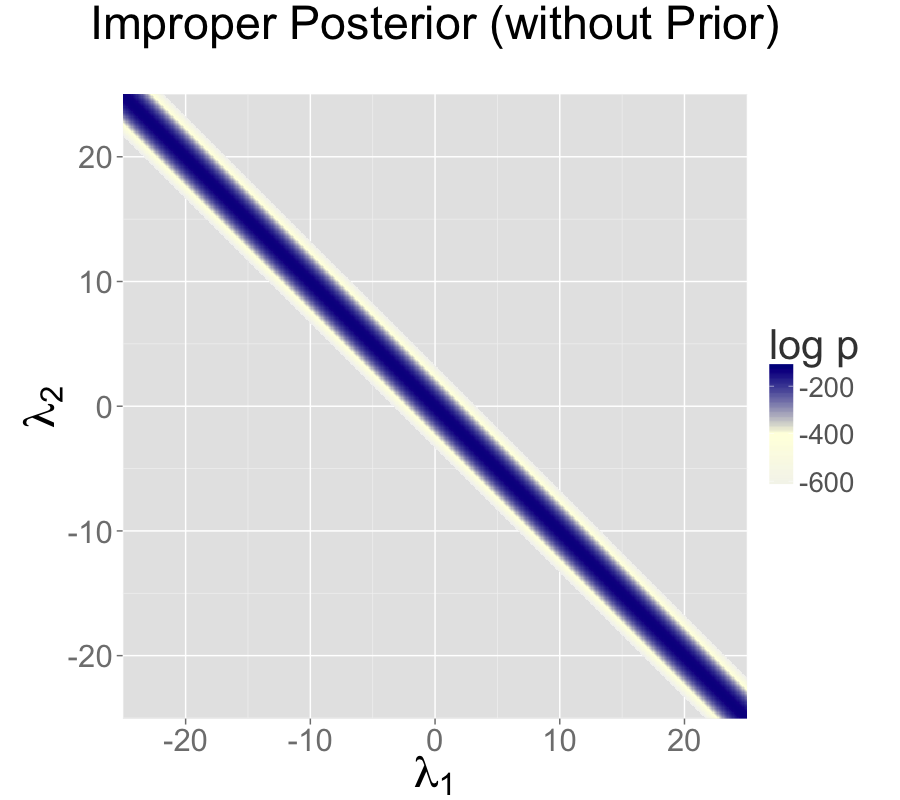
\includegraphics{img/non-identified.png}
\caption{Two intercepts with improper prior}
\end{figure}

Adding a standard normal prior for the intercepts results in a proper posterior.

\begin{figure}
\centering
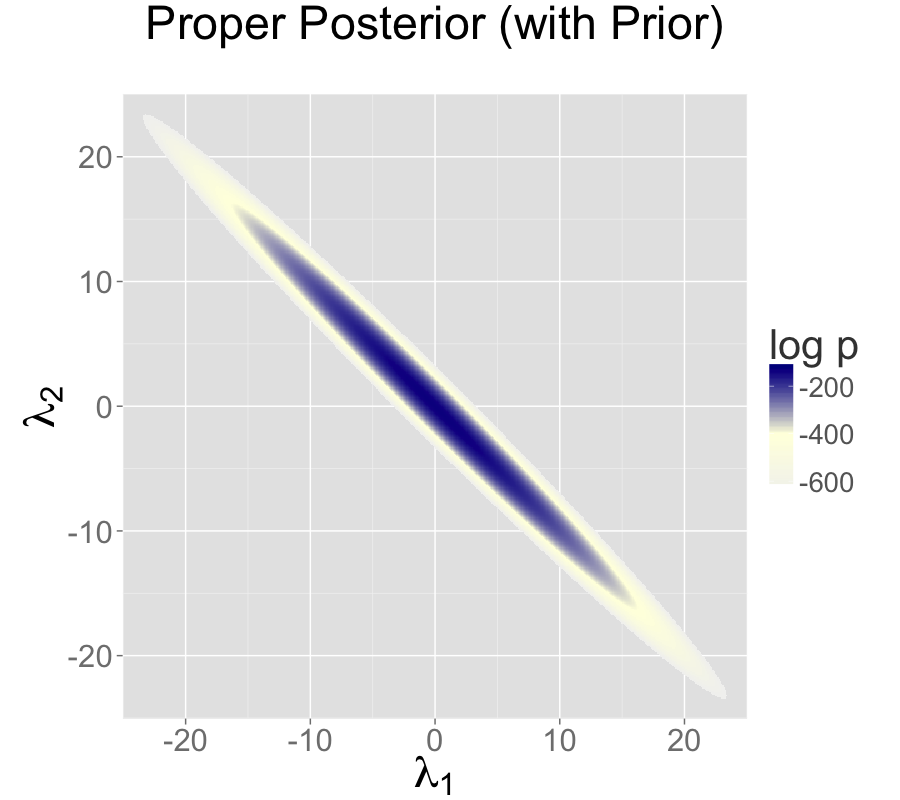
\includegraphics{img/non-identified-plus-prior.png}
\caption{Two intercepts with proper prior}
\end{figure}

The single intercept parameterization with no prior also has a proper posterior.

\begin{figure}
\centering
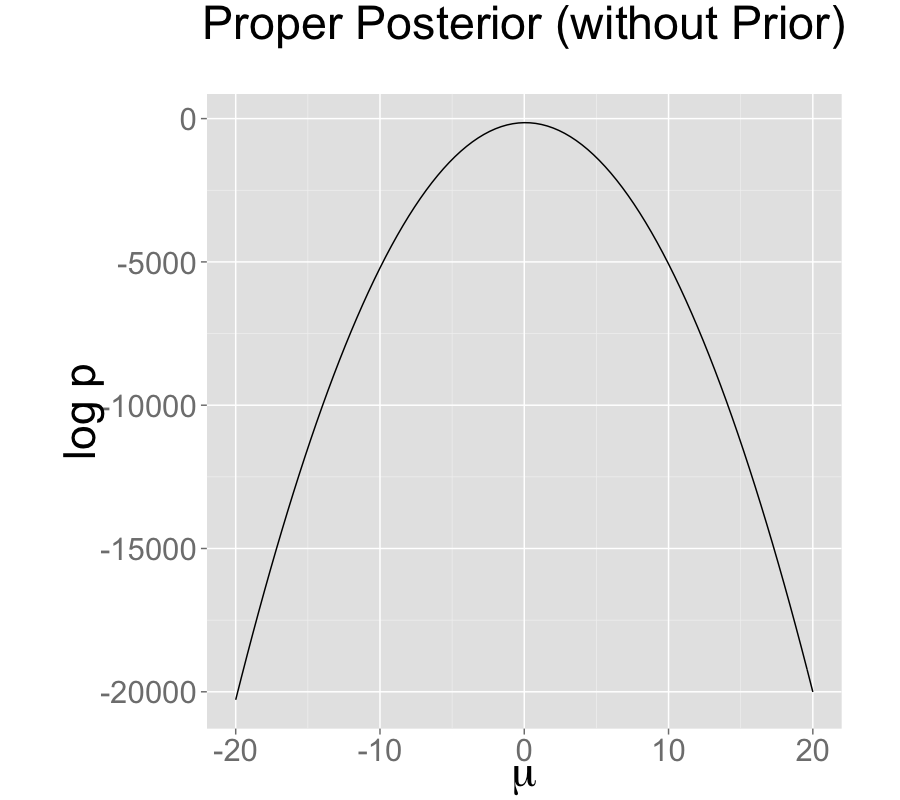
\includegraphics{img/one-param-identified.png}
\caption{Single intercepts with improper prior}
\end{figure}

The addition of a prior to the two intercepts model is shown in the
second plot; the final plot shows the result of reparameterizing to a
single intercept.

An alternative strategy for identifying a \(K\)-simplex parameterization
\(\theta = \texttt{softmax}(\alpha)\) in terms of an unconstrained
\(K\)-vector \(\alpha\) is to place a prior on the components of \(\alpha\)
with a fixed location (that is, specifically avoid hierarchical priors
with varying location). Unlike the approaching of pinning \(\alpha_K = 0\), the prior-based approach models the \(K\) outcomes symmetrically
rather than modeling \(K-1\) outcomes relative to the \(K\)-th. The
pinned parameterization, on the other hand, is usually more efficient
statistically because it does not have the extra degree of (prior
constrained) wiggle room.

\hypertarget{vague-strongly-informative-and-weakly-informative-priors}{%
\subsubsection*{Vague, strongly informative, and weakly informative priors}\label{vague-strongly-informative-and-weakly-informative-priors}}
\addcontentsline{toc}{subsubsection}{Vague, strongly informative, and weakly informative priors}

Care must be used when adding a prior to resolve invariances. If the
prior is taken to be too broad (i.e., too vague), the resolution is in
theory only, and samplers will still struggle.

Ideally, a realistic prior will be formulated based on substantive
knowledge of the problem being modeled. Such a prior can be chosen to
have the appropriate strength based on prior knowledge. A strongly
informative prior makes sense if there is strong prior information.

When there is not strong prior information, a weakly informative prior
strikes the proper balance between controlling computational inference
without dominating the data in the posterior. In most problems, the
modeler will have at least some notion of the expected scale of the
estimates and be able to choose a prior for identification purposes
that does not dominate the data, but provides sufficient computational
control on the posterior.

Priors can also be used in the same way to control the additive
invariance of the IRT model. A typical approach is to place a strong
prior on student ability parameters \(\alpha\) to control scale simply
to control the additive invariance of the basic IRT model and the
multiplicative invariance of the model extended with a item
discrimination parameters; such a prior does not add any prior
knowledge to the problem. Then a prior on item difficulty can be
chosen that is either informative or weakly informative based on prior
knowledge of the problem.

\hypertarget{label-switching-problematic.section}{%
\section{Label switching in mixture models}\label{label-switching-problematic.section}}

Where collinearity in regression models can lead to infinitely many
posterior maxima, swapping components in a mixture model leads to
finitely many posterior maxima.

\hypertarget{mixture-models}{%
\subsection*{Mixture models}\label{mixture-models}}
\addcontentsline{toc}{subsection}{Mixture models}

Consider a normal mixture model with two location parameters \(\mu_1\)
and \(\mu_2\), a shared scale \(\sigma > 0\), a mixture ratio \(\theta \in [0,1]\), and likelihood
\[
p(y \mid \theta,\mu_1,\mu_2,\sigma)
= \prod_{n=1}^N \big( \theta \, \textsf{normal}(y_n \mid \mu_1,\sigma)
                       + (1 - \theta) \, \textsf{normal}(y_n \mid \mu_2,\sigma) \big).
\]
The issue here is exchangeability of the mixture components, because
\[
p(\theta,\mu_1,\mu_2,\sigma \mid y) = p\big((1-\theta),\mu_2,\mu_1,\sigma \mid y\big).
\]
The problem is exacerbated as the number of mixture components \(K\)
grows, as in clustering models, leading to \(K!\) identical posterior
maxima.

\hypertarget{convergence-monitoring-and-effective-sample-size}{%
\subsection*{Convergence monitoring and effective sample size}\label{convergence-monitoring-and-effective-sample-size}}
\addcontentsline{toc}{subsection}{Convergence monitoring and effective sample size}

The analysis of posterior convergence and effective sample size is
also difficult for mixture models. For example, the \(\hat{R}\)
convergence statistic reported by Stan and the computation of
effective sample size are both compromised by label switching. The
problem is that the posterior mean, a key ingredient in these
computations, is affected by label switching, resulting in a posterior
mean for \(\mu_1\) that is equal to that of \(\mu_2\), and a posterior
mean for \(\theta\) that is always 1/2, no matter what the data are.

\hypertarget{some-inferences-are-invariant}{%
\subsection*{Some inferences are invariant}\label{some-inferences-are-invariant}}
\addcontentsline{toc}{subsection}{Some inferences are invariant}

In some sense, the index (or label) of a mixture component is
irrelevant. Posterior predictive inferences can still be carried out
without identifying mixture components. For example, the log
probability of a new observation does not depend on the identities of
the mixture components. The only sound Bayesian inferences in such
models are those that are invariant to label switching. Posterior
means for the parameters are meaningless because they are not
invariant to label switching; for example, the posterior mean for
\(\theta\) in the two component mixture model will always be 1/2.

\hypertarget{highly-multimodal-posteriors}{%
\subsection*{Highly multimodal posteriors}\label{highly-multimodal-posteriors}}
\addcontentsline{toc}{subsection}{Highly multimodal posteriors}

Theoretically, this should not present a problem for inference because
all of the integrals involved in posterior predictive inference will
be well behaved. The problem in practice is computation.

Being able to carry out such invariant inferences in practice is an
altogether different matter. It is almost always intractable to find
even a single posterior mode, much less balance the exploration of the
neighborhoods of multiple local maxima according to the probability
masses. In Gibbs sampling, it is unlikely for \(\mu_1\)
to move to a new mode when sampled conditioned on the current values
of \(\mu_2\) and \(\theta\). For HMC and NUTS, the problem is that the
sampler gets stuck in one of the two ``bowls'' around the modes and
cannot gather enough energy from random momentum assignment to move
from one mode to another.

Even with a proper posterior, all known sampling and inference
techniques are notoriously ineffective when the number of modes grows
super-exponentially as it does for mixture models with increasing
numbers of components.

\hypertarget{hacks-as-fixes}{%
\subsection*{Hacks as fixes}\label{hacks-as-fixes}}
\addcontentsline{toc}{subsection}{Hacks as fixes}

Several hacks (i.e., ``tricks'') have been suggested and employed to
deal with the problems posed by label switching in practice.

\hypertarget{parameter-ordering-constraints}{%
\subsubsection*{Parameter ordering constraints}\label{parameter-ordering-constraints}}
\addcontentsline{toc}{subsubsection}{Parameter ordering constraints}

One common strategy is to impose a constraint on the parameters that
identifies the components. For instance, we might consider
constraining \(\mu_1 < \mu_2\) in the two-component normal mixture model
discussed above. A problem that can arise from such an approach is
when there is substantial probability mass for the opposite ordering
\(\mu_1 > \mu_2\). In these cases, the posteriors are affected by
the constraint and true posterior uncertainty in \(\mu_1\) and \(\mu_2\)
is not captured by the model with the constraint. In addition,
standard approaches to posterior inference for event probabilities is
compromised. For instance, attempting to use \(M\) posterior samples to
estimate \(\textsf{Pr}[\mu_1 > \mu_2]\), will fail, because the estimator
\[
\textsf{Pr}[\mu_1 > \mu_2]
\approx
\sum_{m=1}^M \textrm{I}\left(\mu_1^{(m)} > \mu_2^{(m)}\right)
\]
will result in an estimate of 0 because the posterior respects the
constraint in the model.

\hypertarget{initialization-around-a-single-mode}{%
\subsubsection*{Initialization around a single mode}\label{initialization-around-a-single-mode}}
\addcontentsline{toc}{subsubsection}{Initialization around a single mode}

Another common approach is to run a single chain or to initialize the
parameters near realistic values.\footnote{Tempering methods may be viewed as automated ways to carry
  out such a search for modes, though most MCMC tempering methods
  continue to search for modes on an ongoing basis; see
  (\protect\hyperlink{ref-SwendsenWang:1986}{Swendsen and Wang 1986}; \protect\hyperlink{ref-Neal:1996b}{Neal 1996b}).}

This can work better than the hard constraint approach if reasonable
initial values can be found and the labels do not switch within a
Markov chain. The result is that all chains are glued to a
neighborhood of a particular mode in the posterior.

\hypertarget{component-collapsing-in-mixture-models}{%
\section{Component collapsing in mixture models}\label{component-collapsing-in-mixture-models}}

It is possible for two mixture components in a mixture model to
collapse to the same values during sampling or optimization. For
example, a mixture of \(K\) normals might devolve to have \(\mu_i = \mu_j\) and \(\sigma_i = \sigma_j\) for \(i \neq j\).

This will typically happen early in sampling due to initialization in
MCMC or optimization or arise from random movement during MCMC. Once
the parameters match for a given draw \((m)\), it can become hard to
escape because there can be a trough of low-density mass between the
current parameter values and the ones without collapsed components.

It may help to use a smaller step size during warmup, a stronger prior
on each mixture component's membership responsibility. A more extreme
measure is to include additional mixture components to deal with the
possibility that some of them may collapse.

In general, it is difficult to recover exactly the right \(K\)
mixture components in a mixture model as \(K\) increases beyond one
(yes, even a two-component mixture can have this problem).

\hypertarget{posteriors-with-unbounded-densities}{%
\section{Posteriors with unbounded densities}\label{posteriors-with-unbounded-densities}}

In some cases, the posterior density grows without bounds as
parameters approach certain poles or boundaries. In such, there
are no posterior modes and numerical stability issues can arise as
sampled parameters approach constraint boundaries.

\hypertarget{mixture-models-with-varying-scales}{%
\subsection*{Mixture models with varying scales}\label{mixture-models-with-varying-scales}}
\addcontentsline{toc}{subsection}{Mixture models with varying scales}

One such example is a binary mixture model with scales varying by
component, \(\sigma_1\) and \(\sigma_2\) for locations \(\mu_1\) and
\(\mu_2\). In this situation, the density grows without bound as
\(\sigma_1 \rightarrow 0\) and \(\mu_1 \rightarrow y_n\) for some \(n\);
that is, one of the mixture components concentrates all of its mass
around a single data item \(y_n\).

\hypertarget{beta-binomial-models-with-skewed-data-and-weak-priors}{%
\subsection*{Beta-binomial models with skewed data and weak priors}\label{beta-binomial-models-with-skewed-data-and-weak-priors}}
\addcontentsline{toc}{subsection}{Beta-binomial models with skewed data and weak priors}

Another example of unbounded densities arises with a posterior such as
\(\textsf{beta}(\phi \mid 0.5,0.5)\), which can arise if seemingly weak beta
priors are used for groups that have no data. This density is
unbounded as \(\phi \rightarrow 0\) and \(\phi \rightarrow 1\). Similarly,
a Bernoulli likelihood model coupled with a ``weak'' beta prior, leads
to a posterior
\begin{align*}
p(\phi \mid y)
 &\propto 
   \textsf{beta}(\phi \mid 0.5,0.5) \times \prod_{n=1}^N \textsf{Bernoulli}(y_n \mid \phi) \\
 &=
   \textsf{beta}\left(\phi \,\middle|\, 0.5 + \sum_{n=1}^N y_n, 0.5 + N - \sum_{n=1}^N y_n\right).
\end{align*}

If \(N = 9\) and each \(y_n = 1\), the posterior is
\(\textsf{beta}(\phi \mid 9.5,0,5)\). This posterior is unbounded as \(\phi \rightarrow 1\). Nevertheless, the posterior is proper, and although
there is no posterior mode, the posterior mean is well-defined with a
value of exactly 0.95.

\hypertarget{constrained-vs.-unconstrained-scales}{%
\subsubsection*{Constrained vs.~unconstrained scales}\label{constrained-vs.-unconstrained-scales}}
\addcontentsline{toc}{subsubsection}{Constrained vs.~unconstrained scales}

Stan does not sample directly on the constrained \((0,1)\) space for
this problem, so it doesn't directly deal with unconstrained density
values. Rather, the probability values \(\phi\) are logit-transformed
to \((-\infty,\infty)\). The boundaries at 0 and 1 are pushed out to
\(-\infty\) and \(\infty\) respectively. The Jacobian adjustment that
Stan automatically applies ensures the unconstrained density is
proper. The adjustment for the particular case of \((0,1)\) is \(\log \operatorname{logit}^{-1}(\phi) + \log \operatorname{logit}(1 - \phi)\).

There are two problems that still arise, though. The first is that if
the posterior mass for \(\phi\) is near one of the boundaries, the
logit-transformed parameter will have to sweep out long paths and
thus can dominate the U-turn condition imposed by the no-U-turn
sampler (NUTS). The second issue is that the inverse transform from
the unconstrained space to the constrained space can underflow to 0 or
overflow to 1, even when the unconstrained parameter is not infinite.
Similar problems arise for the expectation terms in logistic
regression, which is why the logit-scale parameterizations of the
Bernoulli and binomial distributions are more stable.

\hypertarget{posteriors-with-unbounded-parameters}{%
\section{Posteriors with unbounded parameters}\label{posteriors-with-unbounded-parameters}}

In some cases, the posterior density will not grow without bound, but
parameters will grow without bound with gradually increasing density
values. Like the models discussed in the previous section that have
densities that grow without bound, such models also have no posterior
modes.

\hypertarget{separability-in-logistic-regression}{%
\subsection*{Separability in logistic regression}\label{separability-in-logistic-regression}}
\addcontentsline{toc}{subsection}{Separability in logistic regression}

Consider a logistic regression model with \(N\) observed outcomes \(y_n \in \{ 0, 1 \}\), an \(N \times K\) matrix \(x\) of predictors, a
\(K\)-dimensional coefficient vector \(\beta\), and sampling distribution
\[
y_n \sim \textsf{Bernoulli}(\operatorname{logit}^{-1}(x_n \beta)).
\]
Now suppose that column \(k\) of the predictor matrix is such that
\(x_{n,k} > 0\) if and only if \(y_n = 1\), a condition known as
``separability.'' In this case, predictive accuracy on the observed data
continue to improve as \(\beta_k \rightarrow \infty\), because for cases
with \(y_n = 1\), \(x_n \beta \rightarrow \infty\) and hence
\(\operatorname{logit}^{-1}(x_n \beta) \rightarrow 1\).

With separability, there is no maximum to the likelihood and hence no
maximum likelihood estimate. From the Bayesian perspective, the
posterior is improper and therefore the marginal posterior mean for
\(\beta_k\) is also not defined. The usual solution to this problem in
Bayesian models is to include a proper prior for \(\beta\), which
ensures a proper posterior.

\hypertarget{uniform-posteriors}{%
\section{Uniform posteriors}\label{uniform-posteriors}}

Suppose your model includes a parameter \(\psi\) that is defined on
\([0,1]\) and is given a flat prior \(\textsf{uniform}(\psi \mid 0,1)\). Now if
the data don't tell us anything about \(\psi\), the posterior is also
\(\textsf{uniform}(\psi \mid 0,1)\).

Although there is no maximum likelihood estimate for \(\psi\), the
posterior is uniform over a closed interval and hence proper. In the
case of a uniform posterior on \([0,1]\), the posterior mean for \(\psi\)
is well-defined with value \(1/2\). Although there is no posterior
mode, posterior predictive inference may nevertheless do the right
thing by simply integrating (i.e., averaging) over the predictions for
\(\psi\) at all points in \([0,1]\).

\hypertarget{sampling-difficulties-with-problematic-priors}{%
\section{Sampling difficulties with problematic priors}\label{sampling-difficulties-with-problematic-priors}}

With an improper posterior, it is theoretically impossible to properly
explore the posterior. However, Gibbs sampling as performed by BUGS
and JAGS, although still unable to properly sample from such an
improper posterior, behaves differently in practice than the
Hamiltonian Monte Carlo sampling performed by Stan when faced with an
example such as the two intercept model discussed in
the \protect\hyperlink{collinearity.section}{collinearity section} and illustrated in
the non-identifiable density plot.

\hypertarget{gibbs-sampling}{%
\subsection*{Gibbs sampling}\label{gibbs-sampling}}
\addcontentsline{toc}{subsection}{Gibbs sampling}

Gibbs sampling, as performed by BUGS and JAGS, may appear to be
efficient and well behaved for this unidentified model, but as
discussed in the previous subsection, will not actually explore the
posterior properly.

Consider what happens with initial values \(\lambda_1^{(0)}, \lambda_2^{(0)}\).
Gibbs sampling proceeds in iteration \(m\) by drawing
\begin{align*}
\lambda_1^{(m)} &\sim p(\lambda_1 \mid \lambda_2^{(m-1)}, \sigma^{(m-1)},  y) \\
\lambda_2^{(m)} &\sim p(\lambda_2 \mid \lambda_1^{(m)},   \sigma^{(m-1)},  y) \\
\sigma^{(m)}    &\sim p(\sigma    \mid \lambda_1^{(m)},   \lambda_2^{(m)}, y).
\end{align*}

Now consider the draw for \(\lambda_1\) (the draw for \(\lambda_2\) is
symmetric), which is conjugate in this model and thus can be done
efficiently. In this model, the range from which the next \(\lambda_1\)
can be drawn is highly constrained by the current values of
\(\lambda_2\) and \(\sigma\). Gibbs will run quickly and provide
seemingly reasonable inferences for \(\lambda_1 + \lambda_2\). But it
will not explore the full range of the posterior; it will merely take
a slow random walk from the initial values. This random walk behavior
is typical of Gibbs sampling when posteriors are highly correlated and
the primary reason to prefer Hamiltonian Monte Carlo to Gibbs sampling
for models with parameters correlated in the posterior.

\hypertarget{hamiltonian-monte-carlo-sampling}{%
\subsection*{Hamiltonian Monte Carlo sampling}\label{hamiltonian-monte-carlo-sampling}}
\addcontentsline{toc}{subsection}{Hamiltonian Monte Carlo sampling}

Hamiltonian Monte Carlo (HMC), as performed by Stan, is much more
efficient at exploring posteriors in models where parameters are
correlated in the posterior. In this particular example, the
Hamiltonian dynamics (i.e., the motion of a fictitious particle given
random momentum in the field defined by the negative log posterior) is
going to run up and down along the valley defined by the potential
energy (ridges in log posteriors correspond to valleys in potential
energy). In practice, even with a random momentum for \(\lambda_1\) and
\(\lambda_2\), the gradient of the log posterior is going to adjust for
the correlation and the simulation will run \(\lambda_1\) and
\(\lambda_2\) in opposite directions along the valley corresponding to
the ridge in the posterior log density.

\hypertarget{no-u-turn-sampling}{%
\subsection*{No-U-turn sampling}\label{no-u-turn-sampling}}
\addcontentsline{toc}{subsection}{No-U-turn sampling}

Stan's default no-U-turn sampler (NUTS), is even more efficient at
exploring the posterior (see \protect\hyperlink{ref-Hoffman-Gelman:2014}{Hoffman and Gelman 2014}). NUTS simulates the
motion of the fictitious particle representing the parameter values
until it makes a U-turn, it will be defeated in most cases, as it will
just move down the potential energy valley indefinitely without making
a U-turn. What happens in practice is that the maximum number of
leapfrog steps in the simulation will be hit in many of the
iterations, causing a large number of log probability and
gradient evaluations (1000 if the max tree depth is set to 10, as in
the default). Thus sampling will appear to be slow. This is
indicative of an improper posterior, not a bug in the NUTS algorithm
or its implementation. It is simply not possible to sample from an
improper posterior! Thus the behavior of HMC in general and NUTS
in particular should be reassuring in that it will clearly fail in
cases of improper posteriors, resulting in a clean diagnostic of
sweeping out large paths in the posterior.

Here are results of Stan runs with default parameters fit to
\(N=100\) data points generated from \(y_n \sim \textsf{normal}(0,1)\):

\emph{Two Scale Parameters, Improper Prior}

\begin{verbatim}
Inference for Stan model: improper_stan
Warmup took (2.7, 2.6, 2.9, 2.9) seconds, 11 seconds total
Sampling took (3.4, 3.7, 3.6, 3.4) seconds, 14 seconds total

                  Mean     MCSE   StdDev        5%       95%  N_Eff  N_Eff/s  R_hat
lp__          -5.3e+01  7.0e-02  8.5e-01  -5.5e+01  -5.3e+01    150       11    1.0
n_leapfrog__   1.4e+03  1.7e+01  9.2e+02   3.0e+00   2.0e+03   2987      212    1.0
lambda1        1.3e+03  1.9e+03  2.7e+03  -2.3e+03   6.0e+03    2.1     0.15    5.2
lambda2       -1.3e+03  1.9e+03  2.7e+03  -6.0e+03   2.3e+03    2.1     0.15    5.2
sigma          1.0e+00  8.5e-03  6.2e-02   9.5e-01   1.2e+00     54      3.9    1.1
mu             1.6e-01  1.9e-03  1.0e-01  -8.3e-03   3.3e-01   2966      211    1.0
\end{verbatim}

\emph{Two Scale Parameters, Weak Prior}

\begin{verbatim}
Warmup took (0.40, 0.44, 0.40, 0.36) seconds, 1.6 seconds total
Sampling took (0.47, 0.40, 0.47, 0.39) seconds, 1.7 seconds total

                 Mean     MCSE   StdDev        5%    95%  N_Eff  N_Eff/s  R_hat
lp__              -54  4.9e-02  1.3e+00  -5.7e+01    -53    728      421    1.0
n_leapfrog__      157  2.8e+00  1.5e+02   3.0e+00    511   3085     1784    1.0
lambda1          0.31  2.8e-01  7.1e+00  -1.2e+01     12    638      369    1.0
lambda2         -0.14  2.8e-01  7.1e+00  -1.2e+01     12    638      369    1.0
sigma             1.0  2.6e-03  8.0e-02   9.2e-01    1.2    939      543    1.0
mu               0.16  1.8e-03  1.0e-01  -8.1e-03   0.33   3289     1902    1.0
\end{verbatim}

\emph{One Scale Parameter, Improper Prior}

\begin{verbatim}
Warmup took (0.011, 0.012, 0.011, 0.011) seconds, 0.044 seconds total
Sampling took (0.017, 0.020, 0.020, 0.019) seconds, 0.077 seconds total

                Mean     MCSE  StdDev        5%   50%   95%  N_Eff  N_Eff/s  R_hat
lp__             -54  2.5e-02    0.91  -5.5e+01   -53   -53   1318    17198    1.0
n_leapfrog__     3.2  2.7e-01     1.7   1.0e+00   3.0   7.0     39      507    1.0
mu              0.17  2.1e-03    0.10  -3.8e-03  0.17  0.33   2408    31417    1.0
sigma            1.0  1.6e-03   0.071   9.3e-01   1.0   1.2   2094    27321    1.0
\end{verbatim}

On the top is the non-identified model with improper uniform priors
and likelihood \(y_n \sim \textsf{normal}(\lambda_1 + \lambda_2, \sigma)\).

In the middle is the same likelihood as the middle plus priors
\(\lambda_k \sim \textsf{normal}(0,10)\).

On the bottom is an identified model with an improper prior, with
likelihood \(y_n \sim \textsf{normal}(\mu,\sigma)\). All models
estimate \(\mu\) at roughly 0.16 with low Monte Carlo standard
error, but a high posterior standard deviation of 0.1; the true
value \(\mu=0\) is within the 90\% posterior intervals in all three models.

\hypertarget{examples-fits-in-stan}{%
\subsection*{Examples: fits in Stan}\label{examples-fits-in-stan}}
\addcontentsline{toc}{subsection}{Examples: fits in Stan}

To illustrate the issues with sampling from non-identified and only
weakly identified models, we fit three models with increasing degrees
of identification of their parameters. The posteriors for these
models is illustrated in the non-identifiable density plot. The
first model is the unidentified model with two location parameters and
no priors discussed in the \protect\hyperlink{collinearity.section}{collinearity section}.

\begin{Shaded}
\begin{Highlighting}[]
\KeywordTok{data}\NormalTok{ \{}
  \DataTypeTok{int}\NormalTok{ N;}
  \DataTypeTok{array}\NormalTok{[N] }\DataTypeTok{real}\NormalTok{ y;}
\NormalTok{\}}
\KeywordTok{parameters}\NormalTok{ \{}
  \DataTypeTok{real}\NormalTok{ lambda1;}
  \DataTypeTok{real}\NormalTok{ lambda2;}
  \DataTypeTok{real}\NormalTok{\textless{}}\KeywordTok{lower}\NormalTok{=}\DecValTok{0}\NormalTok{\textgreater{} sigma;}
\NormalTok{\}}
\KeywordTok{transformed parameters}\NormalTok{ \{}
  \DataTypeTok{real}\NormalTok{ mu;}
\NormalTok{  mu = lambda1 + lambda2;}
\NormalTok{\}}
\KeywordTok{model}\NormalTok{ \{}
\NormalTok{  y \textasciitilde{} normal(mu, sigma);}
\NormalTok{\}}
\end{Highlighting}
\end{Shaded}

The second adds priors to the model block for \texttt{lambda1} and
\texttt{lambda2} to the previous model.

\begin{Shaded}
\begin{Highlighting}[]
\NormalTok{lambda1 \textasciitilde{} normal(}\DecValTok{0}\NormalTok{, }\DecValTok{10}\NormalTok{);}
\NormalTok{lambda2 \textasciitilde{} normal(}\DecValTok{0}\NormalTok{, }\DecValTok{10}\NormalTok{);}
\end{Highlighting}
\end{Shaded}

The third involves a single location parameter, but no priors.

\begin{Shaded}
\begin{Highlighting}[]
\KeywordTok{data}\NormalTok{ \{}
  \DataTypeTok{int}\NormalTok{ N;}
  \DataTypeTok{array}\NormalTok{[N] }\DataTypeTok{real}\NormalTok{ y;}
\NormalTok{\}}
\KeywordTok{parameters}\NormalTok{ \{}
  \DataTypeTok{real}\NormalTok{ mu;}
  \DataTypeTok{real}\NormalTok{\textless{}}\KeywordTok{lower}\NormalTok{=}\DecValTok{0}\NormalTok{\textgreater{} sigma;}
\NormalTok{\}}
\KeywordTok{model}\NormalTok{ \{}
\NormalTok{  y \textasciitilde{} normal(mu, sigma);}
\NormalTok{\}}
\end{Highlighting}
\end{Shaded}

All three of the example models were fit in Stan 2.1.0 with default
parameters (1000 warmup iterations, 1000 sampling iterations, NUTS
sampler with max tree depth of 10). The results are shown in the
non-identified fits figure. The key statistics from these outputs are
the following.

\begin{itemize}
\item
  As indicated by \texttt{R\_hat} column, all parameters have
  converged other than \(\lambda_1\) and \(\lambda_2\) in the
  non-identified model.
\item
  The average number of leapfrog steps is roughly 3 in
  the identified model, 150 in the model identified by a weak prior, and
  1400 in the non-identified model.
\item
  The number of effective samples per
  second for \(\mu\) is roughly 31,000 in the identified model, 1,900 in the model
  identified with weakly informative priors, and 200 in the
  non-identified model; the results are similar for \(\sigma\).
\item
  In the non-identified model, the 95\% interval for \(\lambda_1\) is
  (-2300,6000), whereas it is only (-12,12) in the model identified with
  weakly informative priors.
\item
  In all three models, the simulated value of \(\mu=0\) and \(\sigma=1\)
  are well within the posterior 90\% intervals.
\end{itemize}

The first two points, lack of convergence and hitting the maximum
number of leapfrog steps (equivalently maximum tree depth) are
indicative of improper posteriors. Thus rather than covering up the
problem with poor sampling as may be done with Gibbs samplers,
Hamiltonian Monte Carlo tries to explore the posterior and its failure
is a clear indication that something is amiss in the model.

\hypertarget{change-of-variables.chapter}{%
\chapter{Reparameterization and Change of Variables}\label{change-of-variables.chapter}}

Stan supports a direct encoding of reparameterizations.
Stan also supports changes of variables by directly incrementing the
log probability accumulator with the log Jacobian of the transform.

\hypertarget{theoretical-and-practical-background}{%
\section{Theoretical and practical background}\label{theoretical-and-practical-background}}

A Bayesian posterior is technically a probability \emph{measure},
which is a parameterization-invariant, abstract mathematical object.\footnote{This is in contrast to (penalized) maximum likelihood estimates, which are not parameterization invariant.}

Stan's modeling language, on the other hand, defines a probability
\emph{density}, which is a non-unique, parameterization-dependent
function in \(\mathbb{R}^N \rightarrow \mathbb{R}^{+}\). In practice, this
means a given model can be represented different ways in Stan, and
different representations have different computational performances.

As pointed out by Andrew Gelman (\protect\hyperlink{ref-Gelman:2004}{2004}) in a paper discussing the
relation between parameterizations and Bayesian modeling, a change of
parameterization often carries with it suggestions of how the model
might change, because we tend to use certain natural classes of prior
distributions. Thus, it's not \emph{just} that we have a fixed
distribution that we want to sample from, with reparameterizations
being computational aids. In addition, once we reparameterize and add
prior information, the model itself typically changes, often in useful
ways.

\hypertarget{reparameterizations}{%
\section{Reparameterizations}\label{reparameterizations}}

Reparameterizations may be implemented directly using the transformed
parameters block or just in the model block.

\hypertarget{beta-and-dirichlet-priors}{%
\subsection*{Beta and Dirichlet priors}\label{beta-and-dirichlet-priors}}
\addcontentsline{toc}{subsection}{Beta and Dirichlet priors}

The beta and Dirichlet distributions may both be reparameterized from
a vector of counts to use a mean and total count.

\hypertarget{beta-distribution}{%
\subsubsection*{Beta distribution}\label{beta-distribution}}
\addcontentsline{toc}{subsubsection}{Beta distribution}

For example, the Beta distribution is parameterized by two positive
count parameters \(\alpha, \beta > 0\). The following example
illustrates a hierarchical Stan model with a vector of parameters
\texttt{theta} are drawn i.i.d.~for a Beta distribution whose
parameters are themselves drawn from a hyperprior distribution.

\begin{Shaded}
\begin{Highlighting}[]
\KeywordTok{parameters}\NormalTok{ \{}
  \DataTypeTok{real}\NormalTok{\textless{}}\KeywordTok{lower}\NormalTok{=}\DecValTok{0}\NormalTok{\textgreater{} alpha;}
  \DataTypeTok{real}\NormalTok{\textless{}}\KeywordTok{lower}\NormalTok{=}\DecValTok{0}\NormalTok{\textgreater{} beta;}
  \CommentTok{// ...}
\NormalTok{\}}
\KeywordTok{model}\NormalTok{ \{}
\NormalTok{  alpha \textasciitilde{} ...}
\NormalTok{  beta \textasciitilde{} ...}
  \ControlFlowTok{for}\NormalTok{ (n }\ControlFlowTok{in} \DecValTok{1}\NormalTok{:N) \{}
\NormalTok{    theta[n] \textasciitilde{} beta(alpha, beta);}
\NormalTok{  \}}
  \CommentTok{// ...}
\NormalTok{\}}
\end{Highlighting}
\end{Shaded}

It is often more natural to specify hyperpriors in terms of
transformed parameters. In the case of the Beta, the obvious choice
for reparameterization is in terms of a mean parameter
\[
\phi = \alpha / (\alpha + \beta)
\]
and total count parameter
\[
\lambda = \alpha + \beta.
\]
Following @{[}GelmanEtAl:2013, Chapter 5{]} the mean
gets a uniform prior and the count parameter a Pareto prior with
\(p(\lambda) \propto \lambda^{-2.5}\).

\begin{Shaded}
\begin{Highlighting}[]
\KeywordTok{parameters}\NormalTok{ \{}
  \DataTypeTok{real}\NormalTok{\textless{}}\KeywordTok{lower}\NormalTok{=}\DecValTok{0}\NormalTok{, }\KeywordTok{upper}\NormalTok{=}\DecValTok{1}\NormalTok{\textgreater{} phi;}
  \DataTypeTok{real}\NormalTok{\textless{}}\KeywordTok{lower}\NormalTok{=}\FloatTok{0.1}\NormalTok{\textgreater{} lambda;}
  \CommentTok{// ...}
\NormalTok{\}}
\KeywordTok{transformed parameters}\NormalTok{ \{}
  \DataTypeTok{real}\NormalTok{\textless{}}\KeywordTok{lower}\NormalTok{=}\DecValTok{0}\NormalTok{\textgreater{} alpha = lambda * phi;}
  \DataTypeTok{real}\NormalTok{\textless{}}\KeywordTok{lower}\NormalTok{=}\DecValTok{0}\NormalTok{\textgreater{} beta = lambda * (}\DecValTok{1}\NormalTok{ {-} phi);}
  \CommentTok{// ...}
\NormalTok{\}}
\KeywordTok{model}\NormalTok{ \{}
\NormalTok{  phi \textasciitilde{} beta(}\DecValTok{1}\NormalTok{, }\DecValTok{1}\NormalTok{); }\CommentTok{// uniform on phi, could drop}
\NormalTok{  lambda \textasciitilde{} pareto(}\FloatTok{0.1}\NormalTok{, }\FloatTok{1.5}\NormalTok{);}
  \ControlFlowTok{for}\NormalTok{ (n }\ControlFlowTok{in} \DecValTok{1}\NormalTok{:N) \{}
\NormalTok{    theta[n] \textasciitilde{} beta(alpha, beta);}
\NormalTok{  \}}
  \CommentTok{// ...}
\NormalTok{\}}
\end{Highlighting}
\end{Shaded}

The new parameters, \texttt{phi} and \texttt{lambda}, are declared in the
parameters block and the parameters for the Beta distribution,
\texttt{alpha} and \texttt{beta}, are declared and defined in the
transformed parameters block. And If their values are not of interest,
they could instead be defined as local variables in the model as
follows.

\begin{Shaded}
\begin{Highlighting}[]
\KeywordTok{model}\NormalTok{ \{}
  \DataTypeTok{real}\NormalTok{ alpha = lambda * phi}
  \DataTypeTok{real}\NormalTok{ beta = lambda * (}\DecValTok{1}\NormalTok{ {-} phi);}
  \CommentTok{// ...}
  \ControlFlowTok{for}\NormalTok{ (n }\ControlFlowTok{in} \DecValTok{1}\NormalTok{:N) \{}
\NormalTok{    theta[n] \textasciitilde{} beta(alpha, beta);}
\NormalTok{  \}}
  \CommentTok{// ...}
\NormalTok{\}}
\end{Highlighting}
\end{Shaded}

With vectorization, this could be expressed more compactly and
efficiently as follows.

\begin{Shaded}
\begin{Highlighting}[]
\KeywordTok{model}\NormalTok{ \{}
\NormalTok{  theta \textasciitilde{} beta(lambda * phi, lambda * (}\DecValTok{1}\NormalTok{ {-} phi));}
  \CommentTok{// ...}
\NormalTok{\}}
\end{Highlighting}
\end{Shaded}

If the variables \texttt{alpha} and \texttt{beta} are of interest, they
can be defined in the transformed parameter block and then used in the
model.

\hypertarget{jacobians-not-necessary}{%
\subsubsection*{Jacobians not necessary}\label{jacobians-not-necessary}}
\addcontentsline{toc}{subsubsection}{Jacobians not necessary}

Because the transformed parameters are being used, rather than given a
distribution, there is no need to apply a Jacobian adjustment for the
transform. For example, in the beta distribution example,
\texttt{alpha} and \texttt{beta} have the correct posterior distribution.

\hypertarget{dirichlet-priors}{%
\subsubsection*{Dirichlet priors}\label{dirichlet-priors}}
\addcontentsline{toc}{subsubsection}{Dirichlet priors}

The same thing can be done with a Dirichlet, replacing the mean for
the Beta, which is a probability value, with a simplex. Assume there
are \(K > 0\) dimensions being considered (\(K=1\) is trivial and \(K=2\)
reduces to the beta distribution case). The traditional prior is

\begin{Shaded}
\begin{Highlighting}[]
\KeywordTok{parameters}\NormalTok{ \{}
  \DataTypeTok{vector}\NormalTok{[K] alpha;}
  \DataTypeTok{array}\NormalTok{[N] }\DataTypeTok{simplex}\NormalTok{[K] theta;}
  \CommentTok{// ...}
\NormalTok{\}}
\KeywordTok{model}\NormalTok{ \{}
\NormalTok{  alpha \textasciitilde{} }\CommentTok{// ...}
  \ControlFlowTok{for}\NormalTok{ (n }\ControlFlowTok{in} \DecValTok{1}\NormalTok{:N) \{}
\NormalTok{    theta[n] \textasciitilde{} dirichlet(alpha);}
\NormalTok{  \}}
\NormalTok{\}}
\end{Highlighting}
\end{Shaded}

This provides essentially \(K\) degrees of freedom, one for each
dimension of \texttt{alpha}, and it is not obvious how to specify a
reasonable prior for \texttt{alpha}.

An alternative coding is to use the mean, which is a simplex, and a
total count.

\begin{Shaded}
\begin{Highlighting}[]
\KeywordTok{parameters}\NormalTok{ \{}
  \DataTypeTok{simplex}\NormalTok{[K] phi;}
  \DataTypeTok{real}\NormalTok{\textless{}}\KeywordTok{lower}\NormalTok{=}\DecValTok{0}\NormalTok{\textgreater{} kappa;}
  \DataTypeTok{array}\NormalTok{[N] }\DataTypeTok{simplex}\NormalTok{[K] theta;}
  \CommentTok{// ...}
\NormalTok{\}}
\KeywordTok{transformed parameters}\NormalTok{ \{}
  \DataTypeTok{vector}\NormalTok{[K] alpha = kappa * phi;}
  \CommentTok{// ...}
\NormalTok{\}}
\KeywordTok{model}\NormalTok{ \{}
\NormalTok{  phi \textasciitilde{} }\CommentTok{// ...}
\NormalTok{  kappa \textasciitilde{} }\CommentTok{// ...}
  \ControlFlowTok{for}\NormalTok{ (n }\ControlFlowTok{in} \DecValTok{1}\NormalTok{:N) \{}
\NormalTok{    theta[n] \textasciitilde{} dirichlet(alpha);}
\NormalTok{  \}}
  \CommentTok{// ...}
\NormalTok{\}}
\end{Highlighting}
\end{Shaded}

Now it is much easier to formulate priors, because \texttt{phi} is the
expected value of \texttt{theta} and \texttt{kappa} (minus \texttt{K}) is
the strength of the prior mean measured in number of prior observations.

\hypertarget{transforming-unconstrained-priors-probit-and-logit}{%
\subsection*{Transforming unconstrained priors: probit and logit}\label{transforming-unconstrained-priors-probit-and-logit}}
\addcontentsline{toc}{subsection}{Transforming unconstrained priors: probit and logit}

If the variable \(u\) has a \(\textsf{uniform}(0, 1)\) distribution, then
\(\operatorname{logit}(u)\) is distributed as \(\textsf{logistic}(0, 1)\). This
is because inverse logit is the cumulative distribution function (cdf)
for the logistic distribution, so that the logit function itself is
the inverse CDF and thus maps a uniform draw in \((0, 1)\) to a
logistically-distributed quantity.

Things work the same way for the probit case: if \(u\) has a
\(\textsf{uniform}(0, 1)\) distribution, then \(\Phi^{-1}(u)\) has a
\(\textsf{normal}(0, 1)\) distribution. The other way around, if \(v\)
has a \(\textsf{normal}(0, 1)\) distribution, then \(\Phi(v)\) has a
\(\textsf{uniform}(0, 1)\) distribution.

In order to use the probit and logistic as priors on variables
constrained to \((0, 1)\), create an unconstrained variable and
transform it appropriately. For comparison, the following Stan
program fragment declares a \((0, 1)\)-constrained parameter
\texttt{theta} and gives it a beta prior, then uses it as a parameter in
a distribution (here using \texttt{foo} as a placeholder).

\begin{Shaded}
\begin{Highlighting}[]
\KeywordTok{parameters}\NormalTok{ \{}
  \DataTypeTok{real}\NormalTok{\textless{}}\KeywordTok{lower}\NormalTok{=}\DecValTok{0}\NormalTok{, }\KeywordTok{upper}\NormalTok{=}\DecValTok{1}\NormalTok{\textgreater{} theta;}
  \CommentTok{// ...}
\NormalTok{\}}
\KeywordTok{model}\NormalTok{ \{}
\NormalTok{  theta \textasciitilde{} beta(a, b);}
  \CommentTok{// ...}
\NormalTok{  y \textasciitilde{} foo(theta);}
  \CommentTok{// ...}
\NormalTok{\}}
\end{Highlighting}
\end{Shaded}

If the variables \texttt{a} and \texttt{b} are one, then this imposes
a uniform distribution \texttt{theta}. If \texttt{a} and \texttt{b} are
both less than one, then the density on \texttt{theta} has a U shape,
whereas if they are both greater than one, the density of \texttt{theta}
has an inverted-U or more bell-like shape.

Roughly the same result can be achieved with unbounded parameters that
are probit or inverse-logit-transformed. For example,

\begin{Shaded}
\begin{Highlighting}[]
\KeywordTok{parameters}\NormalTok{ \{}
  \DataTypeTok{real}\NormalTok{ theta\_raw;}
  \CommentTok{// ...}
\NormalTok{\}}
\KeywordTok{transformed parameters}\NormalTok{ \{}
  \DataTypeTok{real}\NormalTok{\textless{}}\KeywordTok{lower}\NormalTok{=}\DecValTok{0}\NormalTok{, }\KeywordTok{upper}\NormalTok{=}\DecValTok{1}\NormalTok{\textgreater{} theta = inv\_logit(theta\_raw);}
  \CommentTok{// ...}
\NormalTok{\}}
\KeywordTok{model}\NormalTok{ \{}
\NormalTok{  theta\_raw \textasciitilde{} logistic(mu, sigma);}
  \CommentTok{// ...}
\NormalTok{  y \textasciitilde{} foo(theta);}
  \CommentTok{// ...}
\NormalTok{\}}
\end{Highlighting}
\end{Shaded}

In this model, an unconstrained parameter \texttt{theta\_raw} gets a
logistic prior, and then the transformed parameter \texttt{theta} is
defined to be the inverse logit of \texttt{theta\_raw}. In this
parameterization, \texttt{inv\_logit(mu)} is the mean of the implied
prior on \texttt{theta}. The prior distribution on \texttt{theta} will be
flat if \texttt{sigma} is one and \texttt{mu} is zero, and will be
U-shaped if \texttt{sigma} is larger than one and bell shaped if
\texttt{sigma} is less than one.

When moving from a variable in \((0, 1)\) to a simplex, the same trick
may be performed using the softmax function, which is a multinomial
generalization of the inverse logit function. First, consider a
simplex parameter with a Dirichlet prior.

\begin{Shaded}
\begin{Highlighting}[]
\KeywordTok{parameters}\NormalTok{ \{}
  \DataTypeTok{simplex}\NormalTok{[K] theta;}
  \CommentTok{// ...}
\NormalTok{\}}
\KeywordTok{model}\NormalTok{ \{}
\NormalTok{  theta \textasciitilde{} dirichlet(a);}
  \CommentTok{// ...}
\NormalTok{  y \textasciitilde{} foo(theta);}
\NormalTok{\}}
\end{Highlighting}
\end{Shaded}

Now \texttt{a} is a vector with \texttt{K} rows, but it has the same shape
properties as the pair \texttt{a} and \texttt{b} for a beta; the beta
distribution is just the distribution of the first component of a
Dirichlet with parameter vector \([a b]^{\top}\). To formulate an
unconstrained prior, the exact same strategy works as for the beta.

\begin{Shaded}
\begin{Highlighting}[]
\KeywordTok{parameters}\NormalTok{ \{}
  \DataTypeTok{vector}\NormalTok{[K] theta\_raw;}
  \CommentTok{// ...}
\NormalTok{\}}
\KeywordTok{transformed parameters}\NormalTok{ \{}
  \DataTypeTok{simplex}\NormalTok{[K] theta = softmax(theta\_raw);}
  \CommentTok{// ...}
\NormalTok{\}}
\KeywordTok{model}\NormalTok{ \{}
\NormalTok{  theta\_raw \textasciitilde{} multi\_normal\_cholesky(mu, L\_Sigma);}
\NormalTok{\}}
\end{Highlighting}
\end{Shaded}

The multivariate normal is used for convenience and efficiency with
its Cholesky-factor parameterization. Now the mean is controlled by
\texttt{softmax(mu)}, but we have additional control of covariance
through \texttt{L\_Sigma} at the expense of having on the order of \(K^2\)
parameters in the prior rather than order \(K\). If no covariance is
desired, the number of parameters can be reduced back to \(K\) using a
vectorized normal distribution as follows.

\begin{Shaded}
\begin{Highlighting}[]
\NormalTok{theta\_raw \textasciitilde{} normal(mu, sigma);}
\end{Highlighting}
\end{Shaded}

where either or both of \texttt{mu} and \texttt{sigma} can be vectors.

\hypertarget{changes-of-variables}{%
\section{Changes of variables}\label{changes-of-variables}}

Changes of variables are applied when the transformation of a
parameter is characterized by a distribution. The standard textbook
example is the lognormal distribution, which is the distribution of a
variable \(y > 0\) whose logarithm \(\log y\) has a normal distribution.
The distribution is being assigned to \(\log y\).

The change of variables requires an adjustment to the probability to
account for the distortion caused by the transform. For this to work,
univariate changes of variables must be monotonic and differentiable
everywhere in their support. Multivariate changes of variables must
be injective and differentiable everywhere in their support, and they
must map \(\mathbb{R}^N \rightarrow \mathbb{R}^N\).

The probability must be scaled by a \emph{Jacobian adjustment} equal to
the absolute determinant of the Jacobian of the transform. In the
univariate case, the Jacobian adjustment is simply the absolute
derivative of the transform.

In the case of log normals, if \(y\)'s logarithm is normal with mean
\(\mu\) and deviation \(\sigma\), then the distribution of \(y\) is given by
\[
p(y)
= \textsf{normal}(\log y \mid \mu, \sigma) \, \left| \frac{d}{dy} \log y \right|
= \textsf{normal}(\log y \mid \mu, \sigma) \, \frac{1}{y}.
\]
Stan works on the log scale to prevent underflow, where
\[
\log p(y)
=
\log \textsf{normal}(\log y \mid \mu, \sigma) - \log y.
\]

In Stan, the change of variables can be applied in the sampling
statement. To adjust for the curvature, the log probability
accumulator is incremented with the log absolute derivative of the
transform. The lognormal distribution can thus be implemented
directly in Stan as follows.\footnote{This example is for illustrative purposes only; the recommended way to implement the lognormal distribution in Stan is with the built-in \texttt{lognormal} probability function; see the functions reference manual for details.}

\begin{Shaded}
\begin{Highlighting}[]
\KeywordTok{parameters}\NormalTok{ \{}
  \DataTypeTok{real}\NormalTok{\textless{}}\KeywordTok{lower}\NormalTok{=}\DecValTok{0}\NormalTok{\textgreater{} y;}
  \CommentTok{// ...}
\NormalTok{\}}
\KeywordTok{model}\NormalTok{ \{}
\NormalTok{  log(y) \textasciitilde{} normal(mu, sigma);}
  \KeywordTok{target +=}\NormalTok{ {-}log(y);}
  \CommentTok{// ...}
\NormalTok{\}}
\end{Highlighting}
\end{Shaded}

It is important, as always, to declare appropriate constraints on
parameters; here \texttt{y} is constrained to be positive.

It would be slightly more efficient to define a local variable for the
logarithm, as follows.

\begin{Shaded}
\begin{Highlighting}[]
\KeywordTok{model}\NormalTok{ \{}
  \DataTypeTok{real}\NormalTok{ log\_y;}
\NormalTok{  log\_y = log(y);}
\NormalTok{  log\_y \textasciitilde{} normal(mu, sigma);}
  \KeywordTok{target +=}\NormalTok{ {-}log\_y;}
  \CommentTok{// ...}
\NormalTok{\}}
\end{Highlighting}
\end{Shaded}

If \texttt{y} were declared as data instead of as a parameter, then the
adjustment can be ignored because the data will be constant and Stan
only requires the log probability up to a constant.

\hypertarget{change-of-variables-vs.-transformations}{%
\subsection*{Change of variables vs.~transformations}\label{change-of-variables-vs.-transformations}}
\addcontentsline{toc}{subsection}{Change of variables vs.~transformations}

This section illustrates the difference between a change of variables
and a simple variable transformation. A transformation samples a
parameter, then transforms it, whereas a change of variables
transforms a parameter, then samples it. Only the latter requires a
Jacobian adjustment.

It does not matter whether the probability function is
expressed using a sampling statement, such as

\begin{Shaded}
\begin{Highlighting}[]
\NormalTok{log(y) \textasciitilde{} normal(mu, sigma);}
\end{Highlighting}
\end{Shaded}

or as an increment to the log probability function, as in

\begin{Shaded}
\begin{Highlighting}[]
\KeywordTok{target +=}\NormalTok{ normal\_lpdf(log(y) | mu, sigma);}
\end{Highlighting}
\end{Shaded}

\hypertarget{jacobian-adjustment.section}{%
\subsubsection*{Gamma and inverse gamma distribution}\label{jacobian-adjustment.section}}
\addcontentsline{toc}{subsubsection}{Gamma and inverse gamma distribution}

Like the log normal, the inverse gamma distribution is a distribution
of variables whose inverse has a gamma distribution. This section
contrasts two approaches, first with a transform, then with a change
of variables.

The transform based approach to sampling \texttt{y\_inv} with an inverse
gamma distribution can be coded as follows.

\begin{Shaded}
\begin{Highlighting}[]
\KeywordTok{parameters}\NormalTok{ \{}
  \DataTypeTok{real}\NormalTok{\textless{}}\KeywordTok{lower}\NormalTok{=}\DecValTok{0}\NormalTok{\textgreater{} y;}
\NormalTok{\}}
\KeywordTok{transformed parameters}\NormalTok{ \{}
  \DataTypeTok{real}\NormalTok{\textless{}}\KeywordTok{lower}\NormalTok{=}\DecValTok{0}\NormalTok{\textgreater{} y\_inv;}
\NormalTok{  y\_inv = }\DecValTok{1}\NormalTok{ / y;}
\NormalTok{\}}
\KeywordTok{model}\NormalTok{ \{}
\NormalTok{  y \textasciitilde{} gamma(}\DecValTok{2}\NormalTok{,}\DecValTok{4}\NormalTok{);}
\NormalTok{\}}
\end{Highlighting}
\end{Shaded}

The change-of-variables approach to sampling \texttt{y\_inv} with an
inverse gamma distribution can be coded as follows.

\begin{Shaded}
\begin{Highlighting}[]
\KeywordTok{parameters}\NormalTok{ \{}
  \DataTypeTok{real}\NormalTok{\textless{}}\KeywordTok{lower}\NormalTok{=}\DecValTok{0}\NormalTok{\textgreater{} y\_inv;}
\NormalTok{\}}
\KeywordTok{transformed parameters}\NormalTok{ \{}
  \DataTypeTok{real}\NormalTok{\textless{}}\KeywordTok{lower}\NormalTok{=}\DecValTok{0}\NormalTok{\textgreater{} y;}
\NormalTok{  y = }\DecValTok{1}\NormalTok{ / y\_inv;  }\CommentTok{// change variables}
\NormalTok{\}}
\KeywordTok{model}\NormalTok{ \{}
\NormalTok{  y \textasciitilde{} gamma(}\DecValTok{2}\NormalTok{,}\DecValTok{4}\NormalTok{);}
  \KeywordTok{target +=}\NormalTok{  {-}}\DecValTok{2}\NormalTok{ * log(y\_inv);  }\CommentTok{//  Jacobian adjustment;}
\NormalTok{\}}
\end{Highlighting}
\end{Shaded}

The Jacobian adjustment is the log of the absolute derivative of the
transform, which in this case is

\[
\log \left| \frac{d}{du} \left( \frac{1}{u} \right) \right|
= \log \left| - u^{-2} \right|
= \log u^{-2}
=  -2 \log u.
\]

\hypertarget{multivariate-changes-of-variables}{%
\subsection*{Multivariate changes of variables}\label{multivariate-changes-of-variables}}
\addcontentsline{toc}{subsection}{Multivariate changes of variables}

In the case of a multivariate transform, the log of the absolute
determinant of the Jacobian of the transform must be added to the
log probability accumulator. In Stan, this can be coded as
follows in the general case where the Jacobian is not a full matrix.

\begin{Shaded}
\begin{Highlighting}[]
\KeywordTok{parameters}\NormalTok{ \{}
  \DataTypeTok{vector}\NormalTok{[K] u;      }\CommentTok{// multivariate parameter}
   \CommentTok{// ...}
\NormalTok{\}}
\KeywordTok{transformed parameters}\NormalTok{ \{}
  \DataTypeTok{vector}\NormalTok{[K] v;     }\CommentTok{// transformed parameter}
  \DataTypeTok{matrix}\NormalTok{[K, K] J;   }\CommentTok{// Jacobian matrix of transform}
  \CommentTok{// ... compute v as a function of u ...}
  \CommentTok{// ... compute J[m, n] = d.v[m] / d.u[n] ...}
  \KeywordTok{target +=}\NormalTok{ log(fabs(determinant(J)));}
  \CommentTok{// ...}
\NormalTok{\}}
\KeywordTok{model}\NormalTok{ \{}
\NormalTok{  v \textasciitilde{} }\CommentTok{// ...}
  \CommentTok{// ...}
\NormalTok{\}}
\end{Highlighting}
\end{Shaded}

If the determinant of the Jacobian is known analytically, it will be
more efficient to apply it directly than to call the determinant
function, which is neither efficient nor particularly stable
numerically.

In many cases, the Jacobian matrix will be triangular, so that only
the diagonal elements will be required for the determinant
calculation. Triangular Jacobians arise when each element \texttt{v{[}k{]}}
of the transformed parameter vector only depends on elements
\texttt{u{[}1{]}}, \ldots, \texttt{u{[}k{]}} of the parameter vector. For
triangular matrices, the determinant is the product of the diagonal
elements, so the transformed parameters block of the above model can
be simplified and made more efficient by recoding as follows.

\begin{Shaded}
\begin{Highlighting}[]
\KeywordTok{transformed parameters}\NormalTok{ \{}
  \CommentTok{// ...}
  \DataTypeTok{vector}\NormalTok{[K] J\_diag;  }\CommentTok{// diagonals of Jacobian matrix}
  \CommentTok{// ...}
  \CommentTok{// ... compute J[k, k] = d.v[k] / d.u[k] ...}
  \KeywordTok{target +=}\NormalTok{ sum(log(J\_diag));}
  \CommentTok{// ...}
\NormalTok{\}}
\end{Highlighting}
\end{Shaded}

\hypertarget{vectors-with-varying-bounds}{%
\section{Vectors with varying bounds}\label{vectors-with-varying-bounds}}

Stan allows scalar and non-scalar upper and lower bounds to be declared in the
constraints for a container data type. The transforms are
calculated and their log Jacobians added to the log density accumulator;
the Jacobian calculations are described in detail in the reference
manual chapter on constrained parameter transforms.

\hypertarget{varying-lower-bounds}{%
\subsection*{Varying lower bounds}\label{varying-lower-bounds}}
\addcontentsline{toc}{subsection}{Varying lower bounds}

For example, suppose there is a vector parameter \(\alpha\) with a
vector \(L\) of lower bounds. The simplest way to deal with this if \(L\)
is a constant is to shift a lower-bounded parameter.

\begin{Shaded}
\begin{Highlighting}[]
\KeywordTok{data}\NormalTok{ \{}
  \DataTypeTok{int}\NormalTok{ N;}
  \DataTypeTok{vector}\NormalTok{[N] L;  }\CommentTok{// lower bounds}
  \CommentTok{// ...}
\NormalTok{\}}
\KeywordTok{parameters}\NormalTok{ \{}
  \DataTypeTok{vector}\NormalTok{\textless{}}\KeywordTok{lower}\NormalTok{=L\textgreater{}[N] alpha\_raw;}
  \CommentTok{// ...}
\NormalTok{\}}
\end{Highlighting}
\end{Shaded}

The above is equivalent to manually calculating the vector bounds by the
following.

\begin{Shaded}
\begin{Highlighting}[]
\KeywordTok{data}\NormalTok{ \{}
  \DataTypeTok{int}\NormalTok{ N;}
  \DataTypeTok{vector}\NormalTok{[N] L;  }\CommentTok{// lower bounds}
  \CommentTok{// ...}
\NormalTok{\}}
\KeywordTok{parameters}\NormalTok{ \{}
  \DataTypeTok{vector}\NormalTok{\textless{}}\KeywordTok{lower}\NormalTok{=}\DecValTok{0}\NormalTok{\textgreater{}[N] alpha\_raw;}
  \CommentTok{// ...}
\NormalTok{\}}
\KeywordTok{transformed parameters}\NormalTok{ \{}
  \DataTypeTok{vector}\NormalTok{[N] alpha = L + alpha\_raw;}
  \CommentTok{// ...}
\NormalTok{\}}
\end{Highlighting}
\end{Shaded}

The Jacobian for adding a constant is one, so its log drops out of the
log density.

Even if the lower bound is a parameter rather than data, there is no
Jacobian required, because the transform from \((L, \alpha_{\textrm{raw}})\)
to \((L + \alpha_{\textrm{raw}}, \alpha_{\textrm{raw}})\) produces
a Jacobian derivative matrix with a unit determinant.

It's also possible to implement the transform using arrary or vector
of parameters as bounds (with the requirement that the type of the
variable must match the bound type) in the following.

\begin{Shaded}
\begin{Highlighting}[]
\KeywordTok{data}\NormalTok{ \{}
  \DataTypeTok{int}\NormalTok{ N;}
  \DataTypeTok{vector}\NormalTok{[N] L;  }\CommentTok{// lower bounds}
  \CommentTok{// ...}
\NormalTok{\}}
\KeywordTok{parameters}\NormalTok{ \{}
  \DataTypeTok{vector}\NormalTok{\textless{}}\KeywordTok{lower}\NormalTok{=}\DecValTok{0}\NormalTok{\textgreater{}[N] alpha\_raw;}
  \DataTypeTok{vector}\NormalTok{\textless{}}\KeywordTok{lower}\NormalTok{=L + alpha\_raw\textgreater{}[N] alpha;}
  \CommentTok{// ...}
\NormalTok{\}}
\end{Highlighting}
\end{Shaded}

This is equivalent to directly transforming
an unconstrained parameter and accounting for the Jacobian.

\begin{Shaded}
\begin{Highlighting}[]
\KeywordTok{data}\NormalTok{ \{}
  \DataTypeTok{int}\NormalTok{ N;}
  \DataTypeTok{vector}\NormalTok{[N] L;  }\CommentTok{// lower bounds}
  \CommentTok{// ...}
\NormalTok{\}}
\KeywordTok{parameters}\NormalTok{ \{}
  \DataTypeTok{vector}\NormalTok{[N] alpha\_raw;}
  \CommentTok{// ...}
\NormalTok{\}}
\KeywordTok{transformed parameters}\NormalTok{ \{}
  \DataTypeTok{vector}\NormalTok{[N] alpha = L + exp(alpha\_raw);}
  \CommentTok{// ...}
\NormalTok{\}}
\KeywordTok{model}\NormalTok{ \{}
  \KeywordTok{target +=}\NormalTok{ sum(alpha\_raw);  }\CommentTok{// log Jacobian}
  \CommentTok{// ...}
\NormalTok{\}}
\end{Highlighting}
\end{Shaded}

The adjustment in the log Jacobian determinant of the transform
mapping \(\alpha_{\textrm{raw}}\) to
\(\alpha = L + \exp(\alpha_{\textrm{raw}})\). The details are simple in
this case because the Jacobian is diagonal; see the reference manual
chapter on constrained parameter transforms for full details. Here
\(L\) can even be a vector containing parameters that don't depend on
\(\alpha_{\textrm{raw}}\); if the bounds do depend on
\(\alpha_{\textrm{raw}}\) then a revised Jacobian needs to be calculated
taking into account the dependencies.

\hypertarget{varying-upper-and-lower-bounds}{%
\subsection*{Varying upper and lower bounds}\label{varying-upper-and-lower-bounds}}
\addcontentsline{toc}{subsection}{Varying upper and lower bounds}

Suppose there are lower and upper bounds that vary by parameter.
These can be applied to shift and rescale a parameter constrained to
\((0, 1)\). This is easily accomplished as the following.

\begin{Shaded}
\begin{Highlighting}[]
\KeywordTok{data}\NormalTok{ \{}
  \DataTypeTok{int}\NormalTok{ N;}
  \DataTypeTok{vector}\NormalTok{[N] L;  }\CommentTok{// lower bounds}
  \DataTypeTok{vector}\NormalTok{[N] U;  }\CommentTok{// upper bounds}
  \CommentTok{// ...}
\NormalTok{\}}
\KeywordTok{parameters}\NormalTok{ \{}
  \DataTypeTok{vector}\NormalTok{\textless{}}\KeywordTok{lower}\NormalTok{=L, }\KeywordTok{upper}\NormalTok{=U\textgreater{}[N] alpha;}
  \CommentTok{// ...}
\NormalTok{\}}
\end{Highlighting}
\end{Shaded}

The same may be accomplished by manually constructing
the transform as follows.

\begin{Shaded}
\begin{Highlighting}[]
\KeywordTok{data}\NormalTok{ \{}
  \DataTypeTok{int}\NormalTok{ N;}
  \DataTypeTok{vector}\NormalTok{[N] L;  }\CommentTok{// lower bounds}
  \DataTypeTok{vector}\NormalTok{[N] U;  }\CommentTok{// upper bounds}
  \CommentTok{// ...}
\NormalTok{\}}
\KeywordTok{parameters}\NormalTok{ \{}
  \DataTypeTok{vector}\NormalTok{\textless{}}\KeywordTok{lower}\NormalTok{=}\DecValTok{0}\NormalTok{, }\KeywordTok{upper}\NormalTok{=}\DecValTok{1}\NormalTok{\textgreater{}[N] alpha\_raw;}
  \CommentTok{// ...}
\NormalTok{\}}
\KeywordTok{transformed parameters}\NormalTok{ \{}
  \DataTypeTok{vector}\NormalTok{[N] alpha = L + (U {-} L) .* alpha\_raw;}
\NormalTok{\}}
\end{Highlighting}
\end{Shaded}

The expression \texttt{U\ -\ L} is multiplied by \texttt{alpha\_raw}
elementwise to produce a vector of variables in \((0, U-L)\), then
adding \(L\) results in a variable ranging between \((L, U)\).

In this case, it is important that \(L\) and \(U\) are constants,
otherwise a Jacobian would be required when multiplying by \(U - L\).

\hypertarget{efficiency-tuning.chapter}{%
\chapter{Efficiency Tuning}\label{efficiency-tuning.chapter}}

This chapter provides a grab bag of techniques for optimizing Stan
code, including vectorization, sufficient statistics, and conjugacy.
At a coarse level, efficiency involves both the amount of time
required for a computation and the amount of memory required. For
practical applied statistical modeling, we are mainly concerned with
reducing wall time (how long a program takes as measured by a clock on
the wall) and keeping memory requirements within available bounds.

\hypertarget{what-is-efficiency}{%
\section{What is efficiency?}\label{what-is-efficiency}}

The standard algorithm analyses in computer science measure efficiency
asymptotically as a function of problem size (such as data, number of
parameters, etc.) and typically do not consider constant additive
factors like startup times or multiplicative factors like speed of
operations. In practice, the constant factors are important; if run
time can be cut in half or more, that's a huge gain. This chapter
focuses on both the constant factors involved in efficiency (such as
using built-in matrix operations as opposed to naive loops) and on
asymptotic efficiency factors (such as using linear algorithms instead
of quadratic algorithms in loops).

\hypertarget{efficiency-for-probabilistic-models-and-algorithms}{%
\section{Efficiency for probabilistic models and algorithms}\label{efficiency-for-probabilistic-models-and-algorithms}}

Stan programs express models which are intrinsically statistical in
nature. The algorithms applied to these models may or may not
themselves be probabilistic. For example, given an initial value for
parameters (which may itself be given deterministically or generated
randomly), Stan's optimization algorithm (L-BFGS) for penalized
maximum likelihood estimation is purely deterministic. Stan's
sampling algorithms are based on Markov chain Monte Carlo algorithms,
which are probabilistic by nature at every step. Stan's variational
inference algorithm (ADVI) is probabilistic despite being an
optimization algorithm; the randomization lies in a nested Monte Carlo
calculation for an expected gradient.

With probabilistic algorithms, there will be variation in run times
(and maybe memory usage) based on the randomization involved. For
example, by starting too far out in the tail, iterative algorithms
underneath the hood, such as the solvers for ordinary differential
equations, may take different numbers of steps. Ideally this
variation will be limited; when there is a lot of variation it can be
a sign that there is a problem with the model's parameterization in
a Stan program or with initialization.

A well-behaved Stan program will have low variance between runs with
different random initializations and differently seeded random number
generators. But sometimes an algorithm can get stuck in one part of
the posterior, typically due to high curvature. Such sticking almost
always indicates the need to reparameterize the model. Just throwing
away Markov chains with apparently poor behavior (slow, or stuck) can
lead to bias in posterior estimates. This problem with getting stuck
can often be overcome by lowering the initial step size to avoid
getting stuck during adaptation and increasing the target acceptance
rate in order to target a lower step size. This is because smaller
step sizes allow Stan's gradient-based algorithms to better follow the
curvature in the density or penalized maximum likelihood being fit.

\hypertarget{statistical-vs.-computational-efficiency}{%
\section{Statistical vs.~ computational efficiency}\label{statistical-vs.-computational-efficiency}}

There is a difference between pure computational efficiency and
statistical efficiency for Stan programs fit with sampling-based
algorithms. Computational efficiency measures the amount of time or
memory required for a given step in a calculation, such as an
evaluation of a log posterior or penalized likelihood.

Statistical efficiency typically involves requiring fewer steps in
algorithms by making the statistical formulation of a model better
behaved. The typical way to do this is by applying a change of
variables (i.e., reparameterization) so that sampling algorithms mix
better or optimization algorithms require less adaptation.

\hypertarget{model-conditioning-and-curvature}{%
\section{Model conditioning and curvature}\label{model-conditioning-and-curvature}}

Because Stan's algorithms (other than Riemannian Hamiltonian Monte
Carlo) rely on step-based gradient-based approximations of the density
(or penalized maximum likelihood) being fitted, posterior curvature
not captured by this first-order approximation plays a central role in
determining the statistical efficiency of Stan's algorithms.

A second-order approximation to curvature is provided by the
Hessian, the matrix of second derivatives of the log density \(\log p(\theta)\) with respect to the parameter vector \(\theta\), defined
as
\[
H(\theta) = \nabla \, \nabla \, \log p(\theta \mid y),
\]
so that
\[
H_{i, j}(\theta) = \frac{\partial^2 \log p(\theta \mid y)}
                {\partial \theta_i \ \partial \theta_j}.
\]
For pure penalized maximum likelihood problems, the posterior log
density \(\log p(\theta \mid y)\) is replaced by the penalized likelihood
function \(\mathcal{L}(\theta) = \log p(y \mid \theta) - \lambda(\theta)\).

\hypertarget{condition-number-and-adaptation}{%
\subsection*{Condition number and adaptation}\label{condition-number-and-adaptation}}
\addcontentsline{toc}{subsection}{Condition number and adaptation}

A good gauge of how difficult a problem the curvature presents is
given by the condition number of the Hessian matrix \(H\), which is the
ratio of the largest to the smallest eigenvalue of \(H\) (assuming the
Hessian is positive definite). This essentially measures the
difference between the flattest direction of movement and the most
curved. Typically, the step size of a gradient-based algorithm is
bounded by the most sharply curved direction. With better conditioned
log densities or penalized likelihood functions, it is easier for
Stan's adaptation, especially the diagonal adaptations that are used
as defaults.

\hypertarget{unit-scales-without-correlation}{%
\subsection*{Unit scales without correlation}\label{unit-scales-without-correlation}}
\addcontentsline{toc}{subsection}{Unit scales without correlation}

Ideally, all parameters should be programmed so that they have unit
scale and so that posterior correlation is reduced; together, these
properties mean that there is no rotation or scaling required for
optimal performance of Stan's algorithms. For Hamiltonian Monte
Carlo, this implies a unit mass matrix, which requires no adaptation
as it is where the algorithm initializes. Riemannian Hamiltonian
Monte Carlo performs this conditioning on the fly at every step, but
such conditioning is expensive computationally.

\hypertarget{varying-curvature}{%
\subsection*{Varying curvature}\label{varying-curvature}}
\addcontentsline{toc}{subsection}{Varying curvature}

In all but very simple models (such as multivariate normals), the
Hessian will vary as \(\theta\) varies (an extreme example is Neal's
funnel, as naturally arises in hierarchical models with little or no
data). The more the curvature varies, the harder it is for all of the
algorithms with fixed adaptation parameters (that is, everything but
Riemannian Hamiltonian Monte Carlo) to find adaptations that cover the
entire density well. Many of the variable transforms proposed are
aimed at improving the conditioning of the Hessian and/or making it
more consistent across the relevant portions of the density (or
penalized maximum likelihood function) being fit.

For all of Stan's algorithms, the curvature along the path from the
initial values of the parameters to the solution is relevant. For
penalized maximum likelihood and variational inference, the solution
of the iterative algorithm will be a single point, so this is all that
matters. For sampling, the relevant ``solution'' is the typical set,
which is the posterior volume where almost all draws from the
posterior lies; thus, the typical set contains almost all of the
posterior probability mass.

With sampling, the curvature may vary dramatically between the points
on the path from the initialization point to the typical set and
within the typical set. This is why adaptation needs to run long
enough to visit enough points in the typical set to get a good
first-order estimate of the curvature within the typical set. If
adaptation is not run long enough, sampling within the typical set
after adaptation will not be efficient. We generally recommend at
least one hundred iterations after the typical set is reached (and the
first effective draw is ready to be realized). Whether adaptation has
run long enough can be measured by comparing the adaptation parameters
derived from a set of diffuse initial parameter values.

\hypertarget{reparameterizing-with-a-change-of-variables}{%
\subsection*{Reparameterizing with a change of variables}\label{reparameterizing-with-a-change-of-variables}}
\addcontentsline{toc}{subsection}{Reparameterizing with a change of variables}

Improving statistical efficiency is achieved by reparameterizing the
model so that the same result may be calculated using a density or
penalized maximum likelihood that is better conditioned. Again, see
the example of reparameterizing Neal's funnel for an example, and also
the examples in the \protect\hyperlink{change-of-variables.chapter}{change of variables
chapter}.

One has to be careful in using change-of-variables reparameterizations
when using maximum likelihood estimation, because they can change the
result if the Jacobian term is inadvertently included in the revised
likelihood model.

\hypertarget{well-specified-models}{%
\section{Well-specified models}\label{well-specified-models}}

Model misspecification, which roughly speaking means using a model
that doesn't match the data, can be a major source of slow code. This
can be seen in cases where simulated data according to the model runs
robustly and efficiently, whereas the real data for which it was
intended runs slowly or may even have convergence and mixing issues.
While some of the techniques recommended in the remaining sections of
this chapter may mitigate the problem, the best remedy is a
better model specification.

Counterintuitively, more complicated models often run faster
than simpler models. One common pattern is with a group of parameters
with a wide fixed prior such as \texttt{normal(0,\ 1000)}). This can fit
slowly due to the mismatch between prior and posterior (the prior has
support for values in the hundreds or even thousands, whereas the
posterior may be concentrated near zero). In such cases, replacing
the fixed prior with a hierarchical prior such as \texttt{normal(mu,\ \ \ sigma)}, where \texttt{mu} and \texttt{sigma} are new parameters with
their own hyperpriors, can be beneficial.

\hypertarget{avoiding-validation}{%
\section{Avoiding validation}\label{avoiding-validation}}

Stan validates all of its data structure constraints. For example,
consider a transformed parameter defined to be a covariance matrix and
then used as a covariance parameter in the model block.

\begin{Shaded}
\begin{Highlighting}[]
\KeywordTok{transformed parameters}\NormalTok{ \{}
  \DataTypeTok{cov\_matrix}\NormalTok{[K] Sigma;}
  \CommentTok{// ...}
\NormalTok{\}                               }\CommentTok{// first validation}
\KeywordTok{model}\NormalTok{ \{}
\NormalTok{  y \textasciitilde{} multi\_normal(mu, Sigma);  }\CommentTok{// second validation}
  \CommentTok{// ...}
\NormalTok{\}}
\end{Highlighting}
\end{Shaded}

Because \texttt{Sigma} is declared to be a covariance matrix, it will be
factored at the end of the transformed parameter block to ensure that
it is positive definite. The multivariate normal log density function
also validates that \texttt{Sigma} is positive definite. This test is
expensive, having cubic run time (i.e., \(\mathcal{O}(N^3)\) for
\(N \times N\) matrices), so it should not be done twice.

The test may be avoided by simply declaring \texttt{Sigma} to be a simple
unconstrained matrix.

\begin{Shaded}
\begin{Highlighting}[]
\KeywordTok{transformed parameters}\NormalTok{ \{}
  \DataTypeTok{matrix}\NormalTok{[K, K] Sigma;}
  \CommentTok{// ...}
\NormalTok{\}}
\KeywordTok{model}\NormalTok{ \{}
\NormalTok{  y \textasciitilde{} multi\_normal(mu, Sigma);  }\CommentTok{// only validation}
\NormalTok{\}}
\end{Highlighting}
\end{Shaded}

Now the only validation is carried out by the multivariate normal.

\hypertarget{reparameterization.section}{%
\section{Reparameterization}\label{reparameterization.section}}

Stan's sampler can be slow in sampling from distributions with
difficult posterior geometries. One way to speed up such models is
through reparameterization. In some cases, reparameterization can
dramatically increase effective sample size for the same number of
iterations or even make programs that would not converge well
behaved.

\hypertarget{funnel.figure}{%
\subsection*{Example: Neal's funnel}\label{funnel.figure}}
\addcontentsline{toc}{subsection}{Example: Neal's funnel}

In this section, we discuss a general transform from a centered to a
non-centered parameterization (\protect\hyperlink{ref-papa-et-al:2007}{Papaspiliopoulos, Roberts, and Sköld 2007}).\footnote{This parameterization came to be known on our mailing lists as the ``Matt trick'' after Matt Hoffman, who independently came up with it while fitting hierarchical models in Stan.}

This reparameterization is helpful when there is not much data,
because it separates the hierarchical parameters and lower-level
parameters in the prior.

Neal (\protect\hyperlink{ref-Neal:2003}{2003}) defines a distribution that exemplifies the difficulties of
sampling from some hierarchical models. Neal's example is fairly
extreme, but can be trivially reparameterized in such a way as to make
sampling straightforward. Neal's example has support for \(y \in \mathbb{R}\) and \(x \in \mathbb{R}^9\) with density

\[
p(y,x) = \textsf{normal}(y \mid 0,3) \times \prod_{n=1}^9
\textsf{normal}(x_n \mid 0,\exp(y/2)).
\]

The probability contours are shaped like ten-dimensional funnels. The
funnel's neck is particularly sharp because of the exponential
function applied to \(y\). A plot of the log marginal density of \(y\)
and the first dimension \(x_1\) is shown in the following plot.

The marginal density of Neal's funnel for the upper-level variable \(y\) and one lower-level variable \(x_1\) (see the text for the formula). The blue region has log density greater than -8, the yellow region density greater than -16, and the gray background a density less than -16.

\begin{figure}
\centering
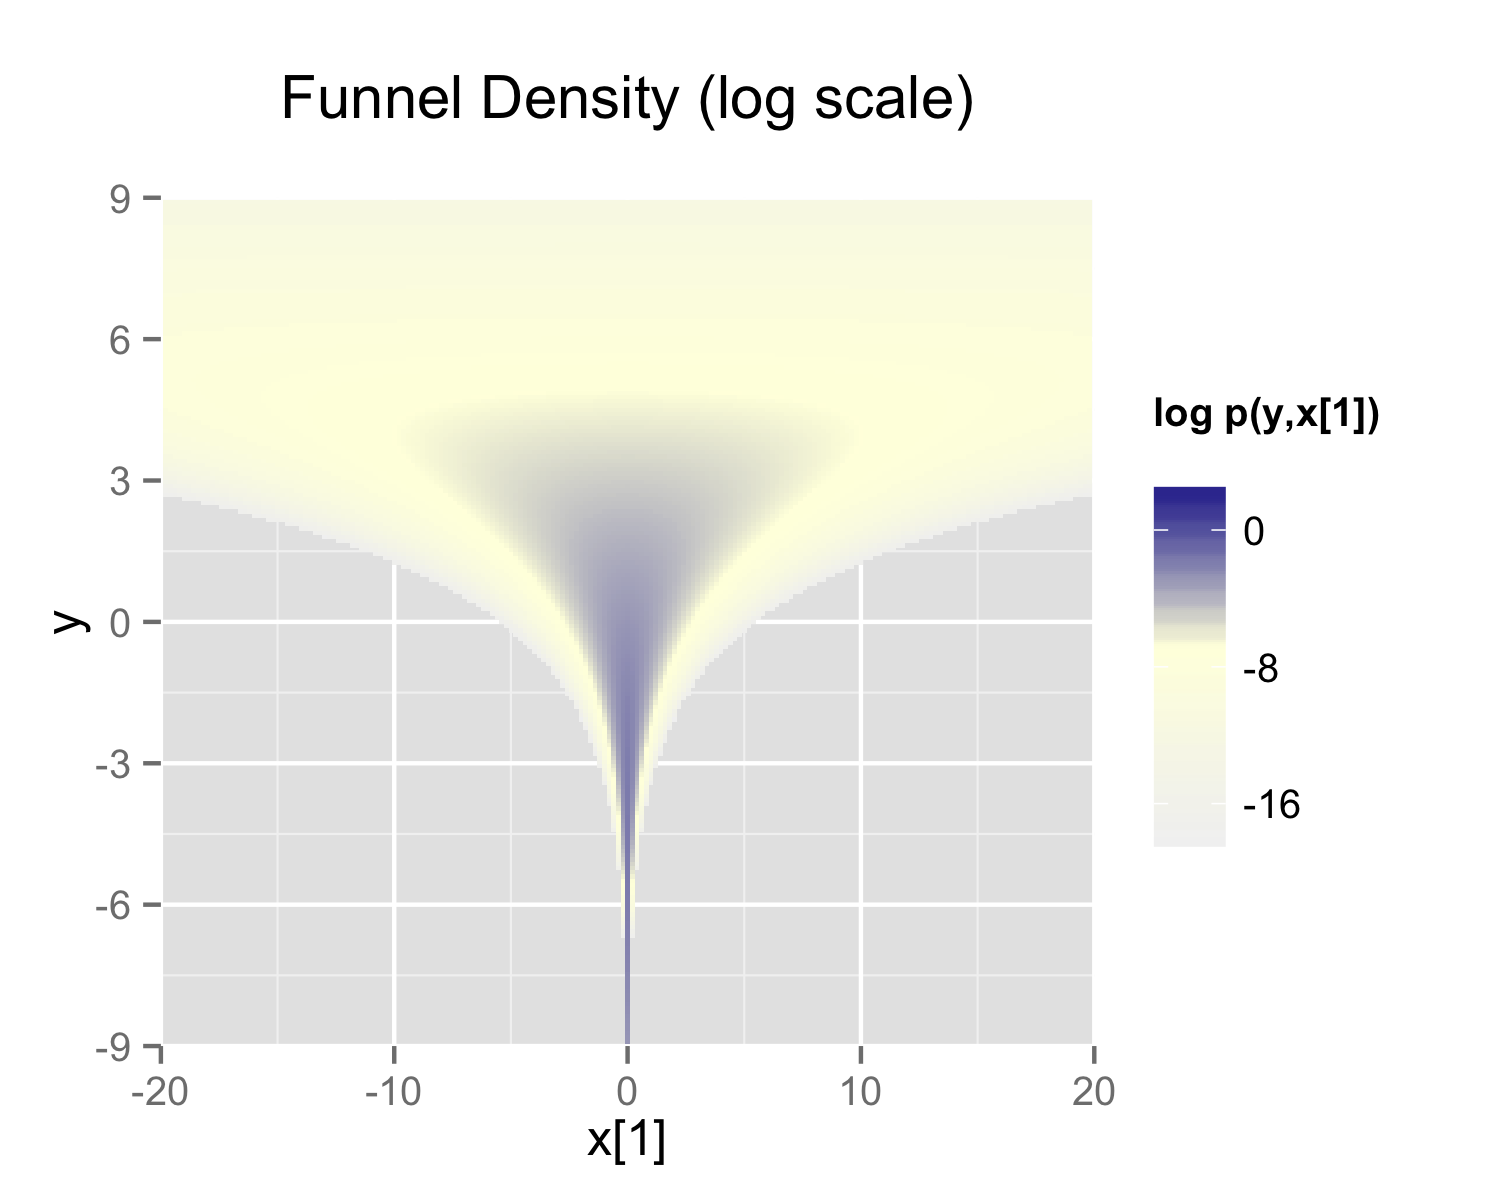
\includegraphics{img/funnel.png}
\caption{Neal's funnel density}
\end{figure}

The funnel can be implemented directly in Stan as follows.

\begin{Shaded}
\begin{Highlighting}[]
\KeywordTok{parameters}\NormalTok{ \{}
  \DataTypeTok{real}\NormalTok{ y;}
  \DataTypeTok{vector}\NormalTok{[}\DecValTok{9}\NormalTok{] x;}
\NormalTok{\}}
\KeywordTok{model}\NormalTok{ \{}
\NormalTok{  y \textasciitilde{} normal(}\DecValTok{0}\NormalTok{, }\DecValTok{3}\NormalTok{);}
\NormalTok{  x \textasciitilde{} normal(}\DecValTok{0}\NormalTok{, exp(y/}\DecValTok{2}\NormalTok{));}
\NormalTok{\}}
\end{Highlighting}
\end{Shaded}

When the model is expressed this way, Stan has trouble sampling from
the neck of the funnel, where \(y\) is small and thus \(x\) is constrained
to be near 0. This is due to the fact that the density's scale
changes with \(y\), so that a step size that works well in the body will
be too large for the neck, and a step size that works in the neck will be
inefficient in the body. This can be seen in the following plot.

4000 draws are taken from a run of Stan's sampler with default settings. Both
plots are restricted to the shown window of \(x_1\) and \(y\) values; some
draws fell outside of the displayed area as would be expected given
the density. The samples are consistent with the marginal density
\(p(y) = \textsf{normal}(y \mid 0,3)\), which has mean 0 and standard
deviation 3.

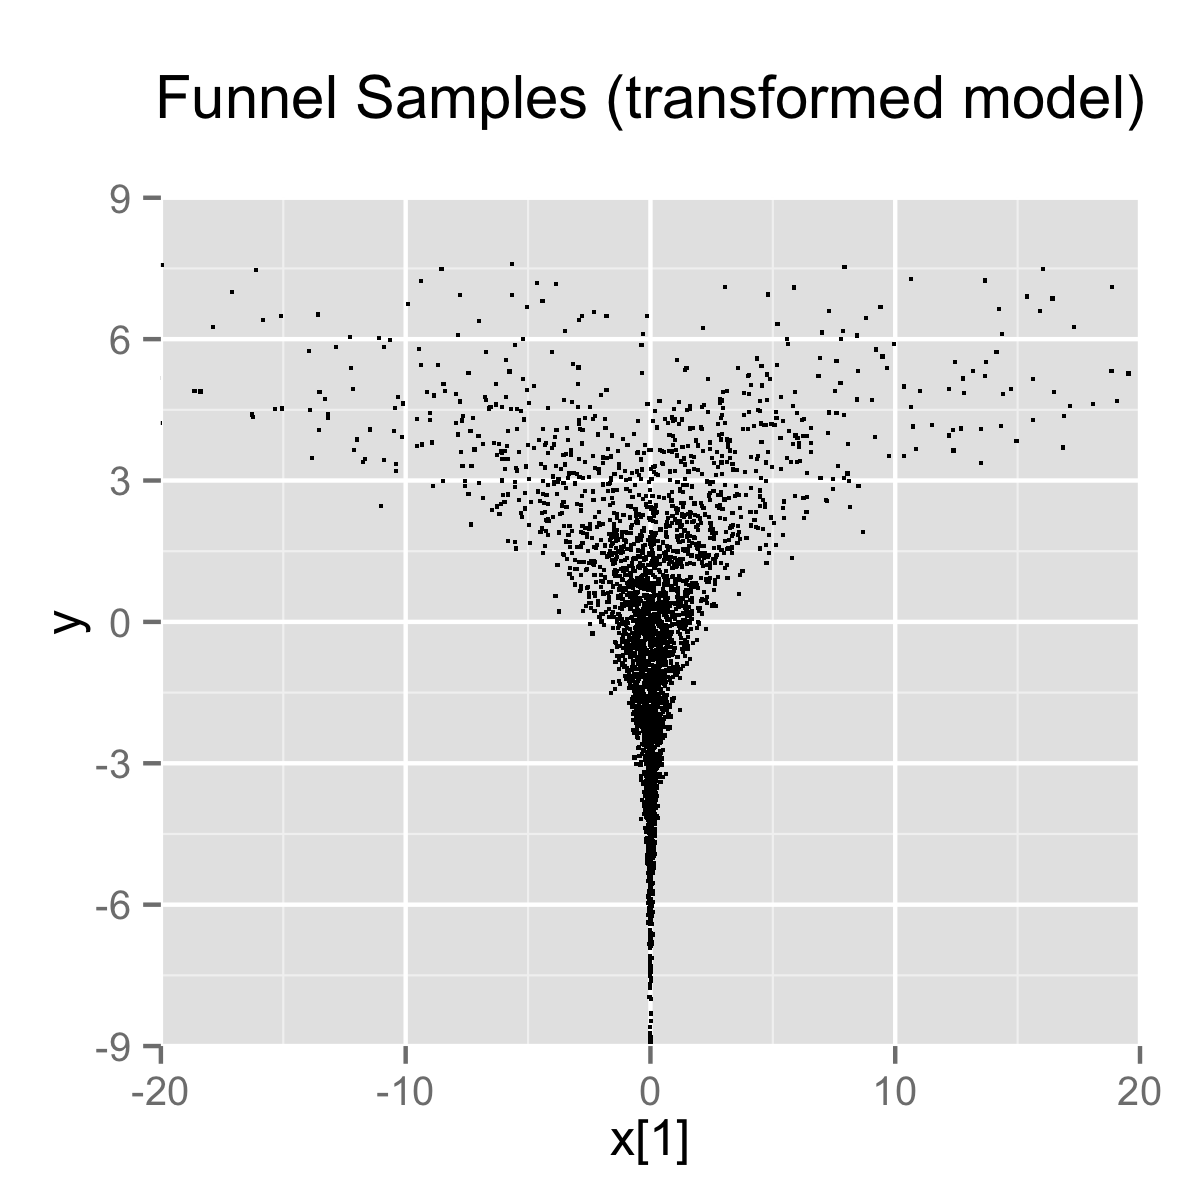
\includegraphics{img/funnel-fit.png}

In this particular instance, because the analytic form of the density
from which samples are drawn is known, the model can be converted to
the following more efficient form.

\begin{Shaded}
\begin{Highlighting}[]
\KeywordTok{parameters}\NormalTok{ \{}
  \DataTypeTok{real}\NormalTok{ y\_raw;}
  \DataTypeTok{vector}\NormalTok{[}\DecValTok{9}\NormalTok{] x\_raw;}
\NormalTok{\}}
\KeywordTok{transformed parameters}\NormalTok{ \{}
  \DataTypeTok{real}\NormalTok{ y;}
  \DataTypeTok{vector}\NormalTok{[}\DecValTok{9}\NormalTok{] x;}

\NormalTok{  y = }\FloatTok{3.0}\NormalTok{ * y\_raw;}
\NormalTok{  x = exp(y/}\DecValTok{2}\NormalTok{) * x\_raw;}
\NormalTok{\}}
\KeywordTok{model}\NormalTok{ \{}
\NormalTok{  y\_raw \textasciitilde{} std\_normal(); }\CommentTok{// implies y \textasciitilde{} normal(0, 3)}
\NormalTok{  x\_raw \textasciitilde{} std\_normal(); }\CommentTok{// implies x \textasciitilde{} normal(0, exp(y/2))}
\NormalTok{\}}
\end{Highlighting}
\end{Shaded}

In this second model, the parameters \texttt{x\_raw} and \texttt{y\_raw} are
sampled as independent standard normals, which is easy for Stan. These
are then transformed into samples from the funnel. In this case, the
same transform may be used to define Monte Carlo samples directly
based on independent standard normal samples; Markov chain Monte Carlo
methods are not necessary. If such a reparameterization were used in
Stan code, it is useful to provide a comment indicating what the
distribution for the parameter implies for the distribution of the
transformed parameter.

\hypertarget{reparameterizing-the-cauchy}{%
\subsection*{Reparameterizing the Cauchy}\label{reparameterizing-the-cauchy}}
\addcontentsline{toc}{subsection}{Reparameterizing the Cauchy}

Sampling from heavy tailed distributions such as the Cauchy is
difficult for Hamiltonian Monte Carlo, which operates within a
Euclidean geometry.\footnote{Riemannian Manifold Hamiltonian Monte Carlo (RMHMC) overcomes this difficulty by simulating the Hamiltonian dynamics in a space with a position-dependent metric; see Girolami and Calderhead (\protect\hyperlink{ref-GirolamiCalderhead:2011}{2011}) and Betancourt (\protect\hyperlink{ref-Betancourt:2012}{2012}).}

The practical problem is that tail of the Cauchy
requires a relatively large step size compared to the trunk. With a
small step size, the No-U-Turn sampler requires many steps when
starting in the tail of the distribution; with a large step size,
there will be too much rejection in the central portion of the
distribution. This problem may be mitigated by defining the
Cauchy-distributed variable as the transform of a uniformly
distributed variable using the Cauchy inverse cumulative distribution
function.

Suppose a random variable of interest \(X\) has a Cauchy distribution
with location \(\mu\) and scale \(\tau\), so that \(X \sim \textsf{Cauchy}(\mu,\tau)\). The variable \(X\) has a cumulative
distribution function \(F_X:\mathbb{R} \rightarrow (0,1)\) defined by
\[
F_X(x) = \frac{1}{\pi} \arctan \left( \frac{x - \mu}{\tau} \right) +
\frac{1}{2}.
\]
The inverse of the cumulative distribution function,
\(F_X^{-1}:(0,1) \rightarrow \mathbb{R}\), is thus

\[
F^{-1}_X(y) = \mu + \tau \tan \left( \pi \left( y - \frac{1}{2} \right) \right).
\]
Thus if the random variable \(Y\) has a unit uniform distribution, \(Y \sim \textsf{uniform}(0,1)\), then \(F^{-1}_X(Y)\) has a Cauchy
distribution with location \(\mu\) and scale \(\tau\), i.e., \(F^{-1}_X(Y) \sim \textsf{Cauchy}(\mu,\tau)\).

Consider a Stan program involving a Cauchy-distributed parameter
\texttt{beta}.

\begin{Shaded}
\begin{Highlighting}[]
\KeywordTok{parameters}\NormalTok{ \{}
  \DataTypeTok{real}\NormalTok{ beta;}
  \CommentTok{// ...}
\NormalTok{\}}
\KeywordTok{model}\NormalTok{ \{}
\NormalTok{  beta \textasciitilde{} cauchy(mu, tau);}
  \CommentTok{// ...}
\NormalTok{\}}
\end{Highlighting}
\end{Shaded}

This declaration of \texttt{beta} as a parameter may be replaced with a
transformed parameter \texttt{beta} defined in terms of a
uniform-distributed parameter \texttt{beta\_unif}.

\begin{Shaded}
\begin{Highlighting}[]
\KeywordTok{parameters}\NormalTok{ \{}
  \DataTypeTok{real}\NormalTok{\textless{}}\KeywordTok{lower}\NormalTok{={-}pi() / }\DecValTok{2}\NormalTok{, }\KeywordTok{upper}\NormalTok{=pi() / }\DecValTok{2}\NormalTok{\textgreater{} beta\_unif;}
  \CommentTok{// ...}
\NormalTok{\}}
\KeywordTok{transformed parameters}\NormalTok{ \{}
  \DataTypeTok{real}\NormalTok{ beta;}
\NormalTok{  beta = mu + tau * tan(beta\_unif);  }\CommentTok{// beta \textasciitilde{} cauchy(mu, tau)}
\NormalTok{\}}
\KeywordTok{model}\NormalTok{ \{}
\NormalTok{  beta\_unif \textasciitilde{} uniform({-}pi() / }\DecValTok{2}\NormalTok{, pi() / }\DecValTok{2}\NormalTok{);  }\CommentTok{// not necessary}
  \CommentTok{// ...}
\NormalTok{\}}
\end{Highlighting}
\end{Shaded}

It is more convenient in Stan to transform a uniform variable on
\((-\pi/2, \pi/2)\) than one on \((0,1)\). The Cauchy location and scale
parameters, \texttt{mu} and \texttt{tau}, may be defined as data or may
themselves be parameters. The variable \texttt{beta} could also be
defined as a local variable if it does not need to be included in the
sampler's output.

The uniform distribution on \texttt{beta\_unif} is defined explicitly in
the model block, but it could be safely removed from the program
without changing sampling behavior. This is because \(\log \textsf{uniform}(\beta_{\textsf{unif}} \mid -\pi/2,\pi/2) = -\log \pi\) is a constant and Stan only
needs the total log probability up to an additive constant. Stan will spend
some time checking that that \texttt{beta\_unif} is between
\texttt{-pi()\ /\ 2} and \texttt{pi()\ /\ 2}, but this condition is guaranteed by
the constraints in the declaration of \texttt{beta\_unif}.

\hypertarget{reparameterizing-a-student-t-distribution}{%
\subsection*{Reparameterizing a Student-t distribution}\label{reparameterizing-a-student-t-distribution}}
\addcontentsline{toc}{subsection}{Reparameterizing a Student-t distribution}

One thing that sometimes works when you're having trouble with the
heavy-tailedness of Student-t distributions is to use the
gamma-mixture representation, which says that you can generate a
Student-t distributed variable \(\beta\),
\[
\beta \sim \textsf{Student-t}(\nu, 0, 1),
\]
by first generating a gamma-distributed precision (inverse variance)
\(\tau\) according to
\[
\tau \sim \textsf{Gamma}(\nu/2, \nu/2),
\]
and then generating \(\beta\) from the normal distribution,
\[
\beta \sim \textsf{normal}\left(0,\tau^{-\frac{1}{2}}\right).
\]

Because \(\tau\) is precision, \(\tau^{-\frac{1}{2}}\) is the scale
(standard deviation), which is the parameterization used by Stan.

The marginal distribution of \(\beta\) when you integrate out \(\tau\) is
\(\textsf{Student-t}(\nu, 0, 1)\), i.e.,
\[
\textsf{Student-t}(\beta \mid \nu, 0, 1)
=
\int_0^{\infty}
\,
\textsf{normal}\left(\beta \middle| 0, \tau^{-0.5}\right)
\times
\textsf{Gamma}\left(\tau \middle| \nu/2, \nu/2\right)
\
\textsf{d} \tau.
\]

To go one step further, instead of defining a \(\beta\) drawn from a
normal with precision \(\tau\), define \(\alpha\) to be drawn from a unit
normal,
\[
\alpha \sim \textsf{normal}(0,1)
\]
and rescale by defining
\[
\beta = \alpha \, \tau^{-\frac{1}{2}}.
\]

Now suppose \(\mu = \beta x\) is the product of \(\beta\) with a
regression predictor \(x\). Then the reparameterization \(\mu = \alpha \tau^{-\frac{1}{2}} x\) has the same distribution, but in the original, direct
parameterization, \(\beta\) has (potentially) heavy tails, whereas in
the second, neither \(\tau\) nor \(\alpha\) have heavy tails.

To translate into Stan notation, this reparameterization replaces

\begin{Shaded}
\begin{Highlighting}[]
\KeywordTok{parameters}\NormalTok{ \{}
  \DataTypeTok{real}\NormalTok{\textless{}}\KeywordTok{lower}\NormalTok{=}\DecValTok{0}\NormalTok{\textgreater{} nu;}
  \DataTypeTok{real}\NormalTok{ beta;}
  \CommentTok{// ...}
\NormalTok{\}}
\KeywordTok{model}\NormalTok{ \{}
\NormalTok{  beta \textasciitilde{} student\_t(nu, }\DecValTok{0}\NormalTok{, }\DecValTok{1}\NormalTok{);}
  \CommentTok{// ...}
\NormalTok{\}}
\end{Highlighting}
\end{Shaded}

with

\begin{Shaded}
\begin{Highlighting}[]
\KeywordTok{parameters}\NormalTok{ \{}
  \DataTypeTok{real}\NormalTok{\textless{}}\KeywordTok{lower}\NormalTok{=}\DecValTok{0}\NormalTok{\textgreater{} nu;}
  \DataTypeTok{real}\NormalTok{\textless{}}\KeywordTok{lower}\NormalTok{=}\DecValTok{0}\NormalTok{\textgreater{} tau;}
  \DataTypeTok{real}\NormalTok{ alpha;}
  \CommentTok{// ...}
\NormalTok{\}}
\KeywordTok{transformed parameters}\NormalTok{ \{}
  \DataTypeTok{real}\NormalTok{ beta;}
\NormalTok{  beta = alpha / sqrt(tau);}
  \CommentTok{// ...}
\NormalTok{\}}
\KeywordTok{model}\NormalTok{ \{}
  \DataTypeTok{real}\NormalTok{ half\_nu;}
\NormalTok{  half\_nu = }\FloatTok{0.5}\NormalTok{ * nu;}
\NormalTok{  tau \textasciitilde{} gamma(half\_nu, half\_nu);}
\NormalTok{  alpha \textasciitilde{} std\_normal();}
  \CommentTok{// ...}
\NormalTok{\}}
\end{Highlighting}
\end{Shaded}

Although set to \texttt{0} here, in most cases, the lower bound for the
degrees of freedom parameter \texttt{nu} can be set to \texttt{1} or
higher; when \texttt{nu} is 1, the result is a Cauchy distribution with
fat tails and as \texttt{nu} approaches infinity, the Student-t
distribution approaches a normal distribution. Thus the parameter
\texttt{nu} characterizes the heaviness of the tails of the model.

\hypertarget{hierarchical-models-and-the-non-centered-parameterization}{%
\subsection*{Hierarchical models and the non-centered parameterization}\label{hierarchical-models-and-the-non-centered-parameterization}}
\addcontentsline{toc}{subsection}{Hierarchical models and the non-centered parameterization}

Unfortunately, the usual situation in applied Bayesian modeling
involves complex geometries and interactions that are not known
analytically. Nevertheless, reparameterization can still be
effective for separating parameters.

\hypertarget{centered-parameterization}{%
\subsubsection*{Centered parameterization}\label{centered-parameterization}}
\addcontentsline{toc}{subsubsection}{Centered parameterization}

For example, a vectorized hierarchical model might draw a vector of
coefficients \(\beta\) with definitions as follows. The so-called
centered parameterization is as follows.

\begin{Shaded}
\begin{Highlighting}[]
\KeywordTok{parameters}\NormalTok{ \{}
  \DataTypeTok{real}\NormalTok{ mu\_beta;}
  \DataTypeTok{real}\NormalTok{\textless{}}\KeywordTok{lower}\NormalTok{=}\DecValTok{0}\NormalTok{\textgreater{} sigma\_beta;}
  \DataTypeTok{vector}\NormalTok{[K] beta;}
  \CommentTok{// ...}
\NormalTok{\}}
\KeywordTok{model}\NormalTok{ \{}
\NormalTok{  beta \textasciitilde{} normal(mu\_beta, sigma\_beta);}
  \CommentTok{// ...}
\NormalTok{\}}
\end{Highlighting}
\end{Shaded}

Although not shown, a full model will have priors on both
\texttt{mu\_beta} and \texttt{sigma\_beta} along with data modeled based on
these coefficients. For instance, a standard binary logistic
regression with data matrix \texttt{x} and binary outcome vector
\texttt{y} would include a likelihood statement such as form
\texttt{y\ \textasciitilde{}\ bernoulli\_logit(x\ *\ beta)}, leading to an analytically
intractable posterior.

A hierarchical model such as the above will suffer from the same kind
of inefficiencies as Neal's funnel, because the values of \texttt{beta},
\texttt{mu\_beta} and \texttt{sigma\_beta} are highly correlated in the
posterior. The extremity of the correlation depends on the amount of
data, with Neal's funnel being the extreme with no data. In these
cases, the non-centered parameterization, discussed in the next
section, is preferable; when there is a lot of data, the centered
parameterization is more efficient. See
Betancourt and Girolami (\protect\hyperlink{ref-Betancourt-Girolami:2013}{2013}) for more information on the effects of
centering in hierarchical models fit with Hamiltonian Monte Carlo.

\hypertarget{non-centered-parameterization}{%
\subsection*{Non-centered parameterization}\label{non-centered-parameterization}}
\addcontentsline{toc}{subsection}{Non-centered parameterization}

Sometimes the group-level effects do not constrain the hierarchical
distribution tightly. Examples arise when there are not many groups,
or when the inter-group variation is high. In such cases,
hierarchical models can be made much more efficient by shifting the
data's correlation with the parameters to the hyperparameters. Similar
to the funnel example, this will be much more efficient in terms of
effective sample size when there is not much data (see
Betancourt and Girolami (\protect\hyperlink{ref-Betancourt-Girolami:2013}{2013})), and in more extreme cases will be
necessary to achieve convergence.

\begin{Shaded}
\begin{Highlighting}[]
\KeywordTok{parameters}\NormalTok{ \{}
  \DataTypeTok{vector}\NormalTok{[K] beta\_raw;}
  \CommentTok{// ...}
\NormalTok{\}}
\KeywordTok{transformed parameters}\NormalTok{ \{}
  \DataTypeTok{vector}\NormalTok{[K] beta;}
  \CommentTok{// implies: beta \textasciitilde{} normal(mu\_beta, sigma\_beta)}
\NormalTok{  beta = mu\_beta + sigma\_beta * beta\_raw;}
\NormalTok{\}}
\KeywordTok{model}\NormalTok{ \{}
\NormalTok{  beta\_raw \textasciitilde{} std\_normal();}
  \CommentTok{// ...}
\NormalTok{\}}
\end{Highlighting}
\end{Shaded}

Any priors defined for \texttt{mu\_beta} and \texttt{sigma\_beta} remain as
defined in the original model.

Reparameterization of hierarchical models is not limited to the normal
distribution, although the normal distribution is the best candidate
for doing so. In general, any distribution of parameters in the
location-scale family is a good candidate for reparameterization. Let
\(\beta = l + s\alpha\) where \(l\) is a location parameter and \(s\) is a
scale parameter. The parameter \(l\) need not be the mean, \(s\) need not
be the standard deviation, and neither the mean nor the standard
deviation need to exist. If \(\alpha\) and \(\beta\) are from the same
distributional family but \(\alpha\) has location zero and unit scale,
while \(\beta\) has location \(l\) and scale \(s\), then that distribution
is a location-scale distribution. Thus, if \(\alpha\) were a parameter
and \(\beta\) were a transformed parameter, then a prior distribution
from the location-scale family on \(\alpha\) with location zero and unit
scale implies a prior distribution on \(\beta\) with location \(l\) and
scale \(s\). Doing so would reduce the dependence between \(\alpha\),
\(l\), and \(s\).

There are several univariate distributions in the location-scale
family, such as the Student t distribution, including its special
cases of the Cauchy distribution (with one degree of freedom) and the
normal distribution (with infinite degrees of freedom). As shown above,
if \(\alpha\) is distributed standard normal, then \(\beta\) is distributed
normal with mean \(\mu = l\) and standard deviation \(\sigma = s\). The
logistic, the double exponential, the generalized extreme value
distributions, and the stable distribution are also in the
location-scale family.

Also, if \(z\) is distributed standard normal, then \(z^2\) is distributed
chi-squared with one degree of freedom. By summing the squares of \(K\)
independent standard normal variates, one can obtain a single variate
that is distributed chi-squared with \(K\) degrees of freedom. However,
for large \(K\), the computational gains of this reparameterization may
be overwhelmed by the computational cost of specifying \(K\) primitive
parameters just to obtain one transformed parameter to use in a model.

\hypertarget{multivariate-reparameterizations}{%
\subsection*{Multivariate reparameterizations}\label{multivariate-reparameterizations}}
\addcontentsline{toc}{subsection}{Multivariate reparameterizations}

The benefits of reparameterization are not limited to univariate
distributions. A parameter with a multivariate normal prior distribution
is also an excellent candidate for reparameterization. Suppose you intend
the prior for \(\beta\) to be multivariate normal with mean vector \(\mu\)
and covariance matrix \(\Sigma\). Such a belief is reflected by the
following code.

\begin{Shaded}
\begin{Highlighting}[]
\KeywordTok{data}\NormalTok{ \{}
  \DataTypeTok{int}\NormalTok{\textless{}}\KeywordTok{lower}\NormalTok{=}\DecValTok{2}\NormalTok{\textgreater{} K;}
  \DataTypeTok{vector}\NormalTok{[K] mu;}
  \DataTypeTok{cov\_matrix}\NormalTok{[K] Sigma;}
  \CommentTok{// ...}
\NormalTok{\}}
\KeywordTok{parameters}\NormalTok{ \{}
  \DataTypeTok{vector}\NormalTok{[K] beta;}
  \CommentTok{// ...}
\NormalTok{\}}
\KeywordTok{model}\NormalTok{ \{}
\NormalTok{  beta \textasciitilde{} multi\_normal(mu, Sigma);}
  \CommentTok{// ...}
\NormalTok{\}}
\end{Highlighting}
\end{Shaded}

In this case \texttt{mu} and \texttt{Sigma} are fixed data, but they could
be unknown parameters, in which case their priors would be unaffected
by a reparameterization of \texttt{beta}.

If \(\alpha\) has the same dimensions as \(\beta\) but the elements of
\(\alpha\) are independently and identically distributed standard normal
such that \(\beta = \mu + L\alpha\), where \(LL^\top = \Sigma\), then
\(\beta\) is distributed multivariate normal with mean vector \(\mu\) and
covariance matrix \(\Sigma\). One choice for \(L\) is the Cholesky factor
of \(\Sigma\). Thus, the model above could be reparameterized as follows.

\begin{Shaded}
\begin{Highlighting}[]
\KeywordTok{data}\NormalTok{ \{}
  \DataTypeTok{int}\NormalTok{\textless{}}\KeywordTok{lower}\NormalTok{=}\DecValTok{2}\NormalTok{\textgreater{} K;}
  \DataTypeTok{vector}\NormalTok{[K] mu;}
  \DataTypeTok{cov\_matrix}\NormalTok{[K] Sigma;}
  \CommentTok{// ...}
\NormalTok{\}}
\KeywordTok{transformed data}\NormalTok{ \{}
  \DataTypeTok{matrix}\NormalTok{[K, K] L;}
\NormalTok{  L = cholesky\_decompose(Sigma);}
\NormalTok{\}}
\KeywordTok{parameters}\NormalTok{ \{}
  \DataTypeTok{vector}\NormalTok{[K] alpha;}
  \CommentTok{// ...}
\NormalTok{\}}
\KeywordTok{transformed parameters}\NormalTok{ \{}
  \DataTypeTok{vector}\NormalTok{[K] beta;}
\NormalTok{  beta = mu + L * alpha;}
\NormalTok{\}}
\KeywordTok{model}\NormalTok{ \{}
\NormalTok{  alpha \textasciitilde{} std\_normal();}
  \CommentTok{// implies: beta \textasciitilde{} multi\_normal(mu, Sigma)}
  \CommentTok{// ...}
\NormalTok{\}}
\end{Highlighting}
\end{Shaded}

This reparameterization is more efficient for two reasons. First, it
reduces dependence among the elements of \texttt{alpha} and second, it
avoids the need to invert \texttt{Sigma} every time \texttt{multi\_normal}
is evaluated.

The Cholesky factor is also useful when a covariance matrix is
decomposed into a correlation matrix that is multiplied from both
sides by a diagonal matrix of standard deviations, where either the
standard deviations or the correlations are unknown parameters. The
Cholesky factor of the covariance matrix is equal to the product of
a diagonal matrix of standard deviations and the Cholesky factor of
the correlation matrix. Furthermore, the product of a diagonal matrix
of standard deviations and a vector is equal to the elementwise
product between the standard deviations and that vector. Thus, if for
example the correlation matrix \texttt{Tau} were fixed data but the
vector of standard deviations \texttt{sigma} were unknown parameters,
then a reparameterization of \texttt{beta} in terms of \texttt{alpha}
could be implemented as follows.

\begin{Shaded}
\begin{Highlighting}[]
\KeywordTok{data}\NormalTok{ \{}
  \DataTypeTok{int}\NormalTok{\textless{}}\KeywordTok{lower}\NormalTok{=}\DecValTok{2}\NormalTok{\textgreater{} K;}
  \DataTypeTok{vector}\NormalTok{[K] mu;}
  \DataTypeTok{corr\_matrix}\NormalTok{[K] Tau;}
  \CommentTok{// ...}
\NormalTok{\}}
\KeywordTok{transformed data}\NormalTok{ \{}
  \DataTypeTok{matrix}\NormalTok{[K, K] L;}
\NormalTok{  L = cholesky\_decompose(Tau);}
\NormalTok{\}}
\KeywordTok{parameters}\NormalTok{ \{}
  \DataTypeTok{vector}\NormalTok{[K] alpha;}
  \DataTypeTok{vector}\NormalTok{\textless{}}\KeywordTok{lower}\NormalTok{=}\DecValTok{0}\NormalTok{\textgreater{}[K] sigma;}
  \CommentTok{// ...}
\NormalTok{\}}
\KeywordTok{transformed parameters}\NormalTok{ \{}
  \DataTypeTok{vector}\NormalTok{[K] beta;}
  \CommentTok{// This equals mu + diag\_matrix(sigma) * L * alpha;}
\NormalTok{  beta = mu + sigma .* (L * alpha);}
\NormalTok{\}}
\KeywordTok{model}\NormalTok{ \{}
\NormalTok{  sigma \textasciitilde{} cauchy(}\DecValTok{0}\NormalTok{, }\DecValTok{5}\NormalTok{);}
\NormalTok{  alpha \textasciitilde{} std\_normal();}
  \CommentTok{// implies: beta \textasciitilde{} multi\_normal(mu,}
  \CommentTok{//  diag\_matrix(sigma) * L * L\textquotesingle{} * diag\_matrix(sigma)))}
  \CommentTok{// ...}
\NormalTok{\}}
\end{Highlighting}
\end{Shaded}

This reparameterization of a multivariate normal distribution in
terms of standard normal variates can be extended to other multivariate
distributions that can be conceptualized as contaminations of the
multivariate normal, such as the multivariate Student t and the skew
multivariate normal distribution.

A Wishart distribution can also be reparameterized in terms of standard
normal variates and chi-squared variates. Let \(L\) be the Cholesky factor
of a \(K \times K\) positive definite scale matrix \(S\) and let \(\nu\) be
the degrees of freedom. If
\[
A = \begin{pmatrix}
\sqrt{c_{1}} & 0            & \cdots                & 0 \\
z_{21}       & \sqrt{c_{2}} & \ddots                & \vdots \\
\vdots       & \ddots       & \ddots                & 0 \\
z_{K1}       & \cdots       & z_{K\left(K-1\right)} & \sqrt{c_{K}}
\end{pmatrix},
\]
where each \(c_i\) is distributed chi-squared with \(\nu - i + 1\) degrees
of freedom and each \(z_{ij}\) is distributed standard normal, then
\(W = LAA^{\top}L^{\top}\) is distributed Wishart with scale matrix
\(S = LL^{\top}\) and degrees of freedom \(\nu\). Such a reparameterization
can be implemented by the following Stan code:

\begin{Shaded}
\begin{Highlighting}[]
\KeywordTok{data}\NormalTok{ \{}
  \DataTypeTok{int}\NormalTok{\textless{}}\KeywordTok{lower}\NormalTok{=}\DecValTok{1}\NormalTok{\textgreater{} N;}
  \DataTypeTok{int}\NormalTok{\textless{}}\KeywordTok{lower}\NormalTok{=}\DecValTok{1}\NormalTok{\textgreater{} K;}
  \DataTypeTok{int}\NormalTok{\textless{}}\KeywordTok{lower}\NormalTok{=K + }\DecValTok{2}\NormalTok{\textgreater{} nu}
  \DataTypeTok{matrix}\NormalTok{[K, K] L; }\CommentTok{// Cholesky factor of scale matrix}
  \DataTypeTok{vector}\NormalTok{[K] mu;}
  \DataTypeTok{matrix}\NormalTok{[N, K] y;}
  \CommentTok{// ...}
\NormalTok{\}}
\KeywordTok{parameters}\NormalTok{ \{}
  \DataTypeTok{vector}\NormalTok{\textless{}}\KeywordTok{lower}\NormalTok{=}\DecValTok{0}\NormalTok{\textgreater{}[K] c;}
  \DataTypeTok{vector}\NormalTok{[}\FloatTok{0.5}\NormalTok{ * K * (K {-} }\DecValTok{1}\NormalTok{)] z;}
  \CommentTok{// ...}
\NormalTok{\}}
\KeywordTok{model}\NormalTok{ \{}
  \DataTypeTok{matrix}\NormalTok{[K, K] A;}
  \DataTypeTok{int}\NormalTok{ count = }\DecValTok{1}\NormalTok{;}
  \ControlFlowTok{for}\NormalTok{ (j }\ControlFlowTok{in} \DecValTok{1}\NormalTok{:(K {-} }\DecValTok{1}\NormalTok{)) \{}
    \ControlFlowTok{for}\NormalTok{ (i }\ControlFlowTok{in}\NormalTok{ (j + }\DecValTok{1}\NormalTok{):K) \{}
\NormalTok{      A[i, j] = z[count];}
\NormalTok{      count += }\DecValTok{1}\NormalTok{;}
\NormalTok{    \}}
    \ControlFlowTok{for}\NormalTok{ (i }\ControlFlowTok{in} \DecValTok{1}\NormalTok{:(j {-} }\DecValTok{1}\NormalTok{)) \{}
\NormalTok{      A[i, j] = }\FloatTok{0.0}\NormalTok{;}
\NormalTok{    \}}
\NormalTok{    A[j, j] = sqrt(c[j]);}
\NormalTok{  \}}
  \ControlFlowTok{for}\NormalTok{ (i }\ControlFlowTok{in} \DecValTok{1}\NormalTok{:(K {-} }\DecValTok{1}\NormalTok{)) \{}
\NormalTok{    A[i, K] = }\DecValTok{0}\NormalTok{;}
\NormalTok{  \}}
\NormalTok{  A[K, K] = sqrt(c[K]);}

  \ControlFlowTok{for}\NormalTok{ (i }\ControlFlowTok{in} \DecValTok{1}\NormalTok{:K) \{}
\NormalTok{    c[i] \textasciitilde{} chi\_square(nu {-} i + }\DecValTok{1}\NormalTok{);}
\NormalTok{  \}}

\NormalTok{  z \textasciitilde{} std\_normal();}
  \CommentTok{// implies: L * A * A\textquotesingle{} * L\textquotesingle{} \textasciitilde{} wishart(nu, L * L\textquotesingle{})}
\NormalTok{  y \textasciitilde{} multi\_normal\_cholesky(mu, L * A);}
  \CommentTok{// ...}
\NormalTok{\}}
\end{Highlighting}
\end{Shaded}

This reparameterization is more efficient for three reasons. First, it
reduces dependence among the elements of \texttt{z} and second, it
avoids the need to invert the covariance matrix, \(W\) every time
\texttt{wishart} is evaluated. Third, if \(W\) is to be used with a
multivariate normal distribution, you can pass \(L A\) to the more
efficient \texttt{multi\_normal\_cholesky} function, rather than passing
\(W\) to \texttt{multi\_normal}.

If \(W\) is distributed Wishart with scale matrix \(S\) and degrees of
freedom \(\nu\), then \(W^{-1}\) is distributed inverse Wishart with inverse
scale matrix \(S^{-1}\) and degrees of freedom \(\nu\). Thus, the previous
result can be used to reparameterize the inverse Wishart distribution.
Since \(W = L A A^{\top} L^{\top}\),
\(W^{-1} = L^{{\top}^{-1}} A^{{\top}^{-1}} A^{-1} L^{-1}\), where all four
inverses exist, but
\(L^{{-1}^{\top}} = L^{{\top}^{-1}}\) and \(A^{{-1}^{\top}} = A^{{\top}^{-1}}\).
We can slightly modify the above Stan code for this case:

\begin{Shaded}
\begin{Highlighting}[]
\KeywordTok{data}\NormalTok{ \{}
  \DataTypeTok{int}\NormalTok{\textless{}}\KeywordTok{lower}\NormalTok{=}\DecValTok{1}\NormalTok{\textgreater{} K;}
  \DataTypeTok{int}\NormalTok{\textless{}}\KeywordTok{lower}\NormalTok{=K + }\DecValTok{2}\NormalTok{\textgreater{} nu}
  \DataTypeTok{matrix}\NormalTok{[K, K] L; }\CommentTok{// Cholesky factor of scale matrix}
  \CommentTok{// ...}
\NormalTok{\}}
\KeywordTok{transformed data}\NormalTok{ \{}
  \DataTypeTok{matrix}\NormalTok{[K, K] eye;}
  \DataTypeTok{matrix}\NormalTok{[K, K] L\_inv;}
  \ControlFlowTok{for}\NormalTok{ (j }\ControlFlowTok{in} \DecValTok{1}\NormalTok{:K) \{}
    \ControlFlowTok{for}\NormalTok{ (i }\ControlFlowTok{in} \DecValTok{1}\NormalTok{:K) \{}
\NormalTok{      eye[i, j] = }\FloatTok{0.0}\NormalTok{;}
\NormalTok{    \}}
\NormalTok{    eye[j, j] = }\FloatTok{1.0}\NormalTok{;}
\NormalTok{  \}}
\NormalTok{  L\_inv = mdivide\_left\_tri\_low(L, eye);}
\NormalTok{\}}
\KeywordTok{parameters}\NormalTok{ \{}
  \DataTypeTok{vector}\NormalTok{\textless{}}\KeywordTok{lower}\NormalTok{=}\DecValTok{0}\NormalTok{\textgreater{}[K] c;}
  \DataTypeTok{vector}\NormalTok{[}\FloatTok{0.5}\NormalTok{ * K * (K {-} }\DecValTok{1}\NormalTok{)] z;}
  \CommentTok{// ...}
\NormalTok{\}}
\KeywordTok{model}\NormalTok{ \{}
  \DataTypeTok{matrix}\NormalTok{[K, K] A;}
  \DataTypeTok{matrix}\NormalTok{[K, K] A\_inv\_L\_inv;}
  \DataTypeTok{int}\NormalTok{ count;}
\NormalTok{  count = }\DecValTok{1}\NormalTok{;}
  \ControlFlowTok{for}\NormalTok{ (j }\ControlFlowTok{in} \DecValTok{1}\NormalTok{:(K {-} }\DecValTok{1}\NormalTok{)) \{}
    \ControlFlowTok{for}\NormalTok{ (i }\ControlFlowTok{in}\NormalTok{ (j + }\DecValTok{1}\NormalTok{):K) \{}
\NormalTok{      A[i, j] = z[count];}
\NormalTok{      count += }\DecValTok{1}\NormalTok{;}
\NormalTok{    \}}
    \ControlFlowTok{for}\NormalTok{ (i }\ControlFlowTok{in} \DecValTok{1}\NormalTok{:(j {-} }\DecValTok{1}\NormalTok{)) \{}
\NormalTok{      A[i, j] = }\FloatTok{0.0}\NormalTok{;}
\NormalTok{    \}}
\NormalTok{    A[j, j] = sqrt(c[j]);}
\NormalTok{  \}}
  \ControlFlowTok{for}\NormalTok{ (i }\ControlFlowTok{in} \DecValTok{1}\NormalTok{:(K {-} }\DecValTok{1}\NormalTok{)) \{}
\NormalTok{    A[i, K] = }\DecValTok{0}\NormalTok{;}
\NormalTok{  \}}
\NormalTok{  A[K, K] = sqrt(c[K]);}

\NormalTok{  A\_inv\_L\_inv = mdivide\_left\_tri\_low(A, L\_inv);}
  \ControlFlowTok{for}\NormalTok{ (i }\ControlFlowTok{in} \DecValTok{1}\NormalTok{:K) \{}
\NormalTok{    c[i] \textasciitilde{} chi\_square(nu {-} i + }\DecValTok{1}\NormalTok{);}
\NormalTok{  \}}

\NormalTok{  z \textasciitilde{} std\_normal(); }\CommentTok{// implies: crossprod(A\_inv\_L\_inv) \textasciitilde{}}
  \CommentTok{// inv\_wishart(nu, L\_inv\textquotesingle{} * L\_inv)}
  \CommentTok{// ...}
\NormalTok{\}}
\end{Highlighting}
\end{Shaded}

Another candidate for reparameterization is the Dirichlet distribution
with all \(K\) shape parameters equal. Zyczkowski and Sommers (\protect\hyperlink{ref-ZyczkowskiSommers:2001}{2001}) shows
that if \(\theta_i\) is equal to the sum of \(\beta\) independent squared
standard normal variates and \(\rho_i = \frac{\theta_i}{\sum \theta_i}\),
then the \(K\)-vector \(\rho\) is distributed Dirichlet with all shape
parameters equal to \(\frac{\beta}{2}\). In particular, if \(\beta = 2\),
then \(\rho\) is uniformly distributed on the unit simplex. Thus, we can
make \(\rho\) be a transformed parameter to reduce dependence, as in:

\begin{Shaded}
\begin{Highlighting}[]
\KeywordTok{data}\NormalTok{ \{}
  \DataTypeTok{int}\NormalTok{\textless{}}\KeywordTok{lower}\NormalTok{=}\DecValTok{1}\NormalTok{\textgreater{} beta;}
  \CommentTok{// ...}
\NormalTok{\}}
\KeywordTok{parameters}\NormalTok{ \{}
  \DataTypeTok{array}\NormalTok{[K] }\DataTypeTok{vector}\NormalTok{[beta] z;}
  \CommentTok{// ...}
\NormalTok{\}}
\KeywordTok{transformed parameters}\NormalTok{ \{}
  \DataTypeTok{simplex}\NormalTok{[K] rho;}
  \ControlFlowTok{for}\NormalTok{ (k }\ControlFlowTok{in} \DecValTok{1}\NormalTok{:K) \{}
\NormalTok{    rho[k] = dot\_self(z[k]); }\CommentTok{// sum{-}of{-}squares}
\NormalTok{  \}}
\NormalTok{  rho = rho / sum(rho);}
\NormalTok{\}}
\KeywordTok{model}\NormalTok{ \{}
  \ControlFlowTok{for}\NormalTok{ (k }\ControlFlowTok{in} \DecValTok{1}\NormalTok{:K) \{}
\NormalTok{    z[k] \textasciitilde{} std\_normal();}
\NormalTok{  \}}
  \CommentTok{// implies: rho \textasciitilde{} dirichlet(0.5 * beta * ones)}
  \CommentTok{// ...}
\NormalTok{\}}
\end{Highlighting}
\end{Shaded}

\hypertarget{vectorization}{%
\section{Vectorization}\label{vectorization}}

\hypertarget{gradient-bottleneck}{%
\subsection*{Gradient bottleneck}\label{gradient-bottleneck}}
\addcontentsline{toc}{subsection}{Gradient bottleneck}

Stan spends the vast majority of its time computing the gradient of
the log probability function, making gradients the obvious target for
optimization. Stan's gradient calculations with algorithmic
differentiation require a template expression to be allocated
and constructed for each subexpression of a Stan program involving
parameters or transformed parameters.\footnote{Stan uses its own arena-based allocation, so allocation and deallocation are faster than with a raw call to \texttt{new}.} This section defines optimization strategies based on vectorizing these subexpressions to reduce the work done during algorithmic differentiation.

\hypertarget{vectorizing-summations}{%
\subsection*{Vectorizing summations}\label{vectorizing-summations}}
\addcontentsline{toc}{subsection}{Vectorizing summations}

Because of the gradient bottleneck described in the previous section,
it is more efficient to collect a sequence of summands into a vector
or array and then apply the \texttt{sum()} operation than it is to
continually increment a variable by assignment and addition. For
example, consider the following code snippet, where \texttt{foo()} is
some operation that depends on \texttt{n}.

\begin{Shaded}
\begin{Highlighting}[]
\ControlFlowTok{for}\NormalTok{ (n }\ControlFlowTok{in} \DecValTok{1}\NormalTok{:N) \{}
\NormalTok{  total += foo(n,...);}
\NormalTok{\}}
\end{Highlighting}
\end{Shaded}

This code has to create intermediate representations for each
of the \texttt{N} summands.

A faster alternative is to copy the values into a vector, then
apply the \texttt{sum()} operator, as in the following refactoring.

\begin{Shaded}
\begin{Highlighting}[]
\NormalTok{\{}
  \DataTypeTok{vector}\NormalTok{[N] summands;}
  \ControlFlowTok{for}\NormalTok{ (n }\ControlFlowTok{in} \DecValTok{1}\NormalTok{:N) \{}
\NormalTok{    summands[n] = foo(n,...);}
\NormalTok{  \}}
\NormalTok{  total = sum(summands);}
\NormalTok{\}}
\end{Highlighting}
\end{Shaded}

Syntactically, the replacement is a statement block delineated
by curly brackets (\texttt{\{}, \texttt{\}}), starting with the definition
of the local variable \texttt{summands}.

Even though it involves extra work to allocate the \texttt{summands}
vector and copy \texttt{N} values into it, the savings in
differentiation more than make up for it. Perhaps surprisingly,
it will also use substantially less memory overall than incrementing
\texttt{total} within the loop.

\hypertarget{vectorization-through-matrix-operations}{%
\subsection*{Vectorization through matrix operations}\label{vectorization-through-matrix-operations}}
\addcontentsline{toc}{subsection}{Vectorization through matrix operations}

The following program directly encodes a linear regression with fixed
unit noise using a two-dimensional array \texttt{x} of predictors, an
array \texttt{y} of outcomes, and an array \texttt{beta} of regression
coefficients.

\begin{Shaded}
\begin{Highlighting}[]
\KeywordTok{data}\NormalTok{ \{}
  \DataTypeTok{int}\NormalTok{\textless{}}\KeywordTok{lower}\NormalTok{=}\DecValTok{1}\NormalTok{\textgreater{} K;}
  \DataTypeTok{int}\NormalTok{\textless{}}\KeywordTok{lower}\NormalTok{=}\DecValTok{1}\NormalTok{\textgreater{} N;}
  \DataTypeTok{array}\NormalTok{[K, N] }\DataTypeTok{real}\NormalTok{ x;}
  \DataTypeTok{array}\NormalTok{[N] }\DataTypeTok{real}\NormalTok{ y;}
\NormalTok{\}}
\KeywordTok{parameters}\NormalTok{ \{}
  \DataTypeTok{array}\NormalTok{[K] }\DataTypeTok{real}\NormalTok{ beta;}
\NormalTok{\}}
\KeywordTok{model}\NormalTok{ \{}
  \ControlFlowTok{for}\NormalTok{ (n }\ControlFlowTok{in} \DecValTok{1}\NormalTok{:N) \{}
    \DataTypeTok{real}\NormalTok{ gamma = }\DecValTok{0}\NormalTok{;}
    \ControlFlowTok{for}\NormalTok{ (k }\ControlFlowTok{in} \DecValTok{1}\NormalTok{:K) \{}
\NormalTok{      gamma += x[n, k] * beta[k];}
\NormalTok{    \}}
\NormalTok{    y[n] \textasciitilde{} normal(gamma, }\DecValTok{1}\NormalTok{);}
\NormalTok{  \}}
\NormalTok{\}}
\end{Highlighting}
\end{Shaded}

The following model computes the same log probability function as the
previous model, even supporting the same input files for data and
initialization.

\begin{Shaded}
\begin{Highlighting}[]
\KeywordTok{data}\NormalTok{ \{}
  \DataTypeTok{int}\NormalTok{\textless{}}\KeywordTok{lower}\NormalTok{=}\DecValTok{1}\NormalTok{\textgreater{} K;}
  \DataTypeTok{int}\NormalTok{\textless{}}\KeywordTok{lower}\NormalTok{=}\DecValTok{1}\NormalTok{\textgreater{} N;}
  \DataTypeTok{array}\NormalTok{[N] }\DataTypeTok{vector}\NormalTok{[K] x;}
  \DataTypeTok{array}\NormalTok{[N] }\DataTypeTok{real}\NormalTok{ y;}
\NormalTok{\}}
\KeywordTok{parameters}\NormalTok{ \{}
  \DataTypeTok{vector}\NormalTok{[K] beta;}
\NormalTok{\}}
\KeywordTok{model}\NormalTok{ \{}
  \ControlFlowTok{for}\NormalTok{ (n }\ControlFlowTok{in} \DecValTok{1}\NormalTok{:N) \{}
\NormalTok{    y[n] \textasciitilde{} normal(dot\_product(x[n], beta), }\DecValTok{1}\NormalTok{);}
\NormalTok{  \}}
\NormalTok{\}}
\end{Highlighting}
\end{Shaded}

Although it produces equivalent results, the dot product should not be
replaced with a transpose and multiply, as in

\begin{Shaded}
\begin{Highlighting}[]
\NormalTok{y[n] \textasciitilde{} normal(x[n]\textquotesingle{} * beta, }\DecValTok{1}\NormalTok{);}
\end{Highlighting}
\end{Shaded}

The relative inefficiency of the transpose and multiply approach is
that the transposition operator allocates a new vector into which the
result of the transposition is copied. This consumes both time
and memory.\footnote{Future versions of Stan may remove this inefficiency by more fully exploiting expression templates inside the Eigen C++ matrix library. This will require enhancing Eigen to deal with mixed-type arguments, such as the type \texttt{double} used for constants and the algorithmic differentiation type \texttt{stan::math::var} used for variables.}

The inefficiency of transposition could itself be mitigated by
reordering the product and pulling the transposition out of the loop,
as follows.

\begin{Shaded}
\begin{Highlighting}[]
\CommentTok{// ...}
\KeywordTok{transformed parameters}\NormalTok{ \{}
  \DataTypeTok{row\_vector}\NormalTok{[K] beta\_t;}
\NormalTok{  beta\_t = beta\textquotesingle{};}
\NormalTok{\}}
\KeywordTok{model}\NormalTok{ \{}
  \ControlFlowTok{for}\NormalTok{ (n }\ControlFlowTok{in} \DecValTok{1}\NormalTok{:N) \{}
\NormalTok{    y[n] \textasciitilde{} normal(beta\_t * x[n], }\DecValTok{1}\NormalTok{);}
\NormalTok{  \}}
\NormalTok{\}}
\end{Highlighting}
\end{Shaded}

The problem with transposition could be completely solved by directly
encoding the \texttt{x} as a row vector, as in the
following example.

\begin{Shaded}
\begin{Highlighting}[]
\KeywordTok{data}\NormalTok{ \{}
  \CommentTok{// ...}
  \DataTypeTok{array}\NormalTok{[N] }\DataTypeTok{row\_vector}\NormalTok{[K] x;}
  \CommentTok{// ...}
\NormalTok{\}}
\KeywordTok{parameters}\NormalTok{ \{}
  \DataTypeTok{vector}\NormalTok{[K] beta;}
\NormalTok{\}}
\KeywordTok{model}\NormalTok{ \{}
  \ControlFlowTok{for}\NormalTok{ (n }\ControlFlowTok{in} \DecValTok{1}\NormalTok{:N) \{}
\NormalTok{    y[n] \textasciitilde{} normal(x[n] * beta, }\DecValTok{1}\NormalTok{);}
\NormalTok{  \}}
\NormalTok{\}}
\end{Highlighting}
\end{Shaded}

Declaring the data as a matrix and then computing all the predictors
at once using matrix multiplication is more efficient still, as in the
example discussed in the next section.

Having said all this, the most efficient way to code this model is
with direct matrix multiplication, as in

\begin{Shaded}
\begin{Highlighting}[]
\KeywordTok{data}\NormalTok{ \{}
  \DataTypeTok{matrix}\NormalTok{[N, K] x;}
  \DataTypeTok{vector}\NormalTok{[N] y;}
\NormalTok{\}}
\KeywordTok{parameters}\NormalTok{ \{}
  \DataTypeTok{vector}\NormalTok{[K] beta;}
\NormalTok{\}}
\KeywordTok{model}\NormalTok{ \{}
\NormalTok{  y \textasciitilde{} normal(x * beta, }\DecValTok{1}\NormalTok{);}
\NormalTok{\}}
\end{Highlighting}
\end{Shaded}

In general, encapsulated single operations that do the work of loops
will be more efficient in their encapsulated forms. Rather than
performing a sequence of row-vector/vector multiplications, it is
better to encapsulate it as a single matrix/vector multiplication.

\hypertarget{vectorized-probability-functions}{%
\subsection*{Vectorized probability functions}\label{vectorized-probability-functions}}
\addcontentsline{toc}{subsection}{Vectorized probability functions}

The final and most efficient version replaces the loops and
transformed parameters by using the vectorized form of the normal
probability function, as in the following example.

\begin{Shaded}
\begin{Highlighting}[]
\KeywordTok{data}\NormalTok{ \{}
  \DataTypeTok{int}\NormalTok{\textless{}}\KeywordTok{lower}\NormalTok{=}\DecValTok{1}\NormalTok{\textgreater{} K;}
  \DataTypeTok{int}\NormalTok{\textless{}}\KeywordTok{lower}\NormalTok{=}\DecValTok{1}\NormalTok{\textgreater{} N;}
  \DataTypeTok{matrix}\NormalTok{[N, K] x;}
  \DataTypeTok{vector}\NormalTok{[N] y;}
\NormalTok{\}}
\KeywordTok{parameters}\NormalTok{ \{}
  \DataTypeTok{vector}\NormalTok{[K] beta;}
\NormalTok{\}}
\KeywordTok{model}\NormalTok{ \{}
\NormalTok{  y \textasciitilde{} normal(x * beta, }\DecValTok{1}\NormalTok{);}
\NormalTok{\}}
\end{Highlighting}
\end{Shaded}

The variables are all declared as either matrix or vector types.
The result of the matrix-vector multiplication \texttt{x\ *\ beta} in the
model block is a vector of the same length as \texttt{y}.

The probability function documentation in the function reference
manual indicates which of Stan's probability functions support
vectorization; see the function reference manual for full details.
Vectorized probability functions accept either vector or scalar inputs
for all arguments, with the only restriction being that all vector
arguments are the same dimensionality. In the example above, \texttt{y} is a
vector of size \texttt{N}, \texttt{x\ *\ beta} is a vector of size \texttt{N}, and \texttt{1} is a
scalar.

\hypertarget{reshaping-data-for-vectorization}{%
\subsection*{Reshaping data for vectorization}\label{reshaping-data-for-vectorization}}
\addcontentsline{toc}{subsection}{Reshaping data for vectorization}

Sometimes data does not arrive in a shape that is ideal for
vectorization, but can be put into such shape with some munging
(either inside Stan's transformed data block or outside).

John Hall provided a simple example on the Stan users group.
Simplifying notation a bit, the original model had a sampling
statement in a loop, as follows.

\begin{Shaded}
\begin{Highlighting}[]
\ControlFlowTok{for}\NormalTok{ (n }\ControlFlowTok{in} \DecValTok{1}\NormalTok{:N) \{}
\NormalTok{  y[n] \textasciitilde{} normal(mu[ii[n]], sigma);}
\NormalTok{\}}
\end{Highlighting}
\end{Shaded}

The brute force vectorization would build up a mean vector and then
vectorize all at once.

\begin{Shaded}
\begin{Highlighting}[]
\NormalTok{\{}
  \DataTypeTok{vector}\NormalTok{[N] mu\_ii;}
  \ControlFlowTok{for}\NormalTok{ (n }\ControlFlowTok{in} \DecValTok{1}\NormalTok{:N) \{}
\NormalTok{    mu\_ii[n] = mu[ii[n]];}
\NormalTok{  \}}
\NormalTok{  y \textasciitilde{} normal(mu\_ii, sigma);}
\NormalTok{\}}
\end{Highlighting}
\end{Shaded}

If there aren't many levels (values \texttt{ii{[}n{]}} can take), then it
behooves us to reorganize the data by group in a case like this.
Rather than having a single observation vector \texttt{y}, there are K of them.
And because Stan doesn't support ragged arrays, it means K
declarations. For instance, with 5 levels, we have

\begin{Shaded}
\begin{Highlighting}[]
\NormalTok{y\_1 \textasciitilde{} normal(mu[}\DecValTok{1}\NormalTok{], sigma);}
\CommentTok{// ...}
\NormalTok{y\_5 \textasciitilde{} normal(mu[}\DecValTok{5}\NormalTok{], sigma);}
\end{Highlighting}
\end{Shaded}

This way, both the \texttt{mu} and \texttt{sigma} parameters are shared.
Which way works out to be more efficient will depend on the shape of
the data; if the sizes are small, the simple vectorization may be
faster, but for moderate to large sized groups, the full expansion
should be faster.

\hypertarget{exploiting-sufficient-statistics}{%
\section{Exploiting sufficient statistics}\label{exploiting-sufficient-statistics}}

In some cases, models can be recoded to exploit sufficient statistics
in estimation. This can lead to large efficiency gains compared to an
expanded model. For example, consider the following Bernoulli
sampling model.

\begin{Shaded}
\begin{Highlighting}[]
\KeywordTok{data}\NormalTok{ \{}
  \DataTypeTok{int}\NormalTok{\textless{}}\KeywordTok{lower}\NormalTok{=}\DecValTok{0}\NormalTok{\textgreater{} N;}
  \DataTypeTok{array}\NormalTok{[N] }\DataTypeTok{int}\NormalTok{\textless{}}\KeywordTok{lower}\NormalTok{=}\DecValTok{0}\NormalTok{, }\KeywordTok{upper}\NormalTok{=}\DecValTok{1}\NormalTok{\textgreater{} y;}
  \DataTypeTok{real}\NormalTok{\textless{}}\KeywordTok{lower}\NormalTok{=}\DecValTok{0}\NormalTok{\textgreater{} alpha;}
  \DataTypeTok{real}\NormalTok{\textless{}}\KeywordTok{lower}\NormalTok{=}\DecValTok{0}\NormalTok{\textgreater{} beta;}
\NormalTok{\}}
\KeywordTok{parameters}\NormalTok{ \{}
  \DataTypeTok{real}\NormalTok{\textless{}}\KeywordTok{lower}\NormalTok{=}\DecValTok{0}\NormalTok{, }\KeywordTok{upper}\NormalTok{=}\DecValTok{1}\NormalTok{\textgreater{} theta;}
\NormalTok{\}}
\KeywordTok{model}\NormalTok{ \{}
\NormalTok{  theta \textasciitilde{} beta(alpha, beta);}
  \ControlFlowTok{for}\NormalTok{ (n }\ControlFlowTok{in} \DecValTok{1}\NormalTok{:N) \{}
\NormalTok{    y[n] \textasciitilde{} bernoulli(theta);}
\NormalTok{  \}}
\NormalTok{\}}
\end{Highlighting}
\end{Shaded}

In this model, the sum of positive outcomes in \texttt{y} is a
sufficient statistic for the chance of success \texttt{theta}. The
model may be recoded using the binomial distribution as follows.

\begin{Shaded}
\begin{Highlighting}[]
\NormalTok{theta \textasciitilde{} beta(alpha, beta);}
\NormalTok{sum(y) \textasciitilde{} binomial(N, theta);}
\end{Highlighting}
\end{Shaded}

Because truth is represented as one and falsehood as zero, the sum
\texttt{sum(y)} of a binary vector \texttt{y} is equal to the number of
positive outcomes out of a total of \texttt{N} trials.

This can be generalized to other discrete cases (one wouldn't expect
continuous observations to be duplicated if they are random). Suppose
there are only \(K\) possible discrete outcomes, \(z_1, \dotsc, z_K\), but
there are \(N\) observations, where \(N\) is much larger than \(K\). If
\(f_k\) is the frequency of outcome \(z_k\), then the entire likelihood
with distribution \texttt{foo} can be coded as follows.

\begin{Shaded}
\begin{Highlighting}[]
\ControlFlowTok{for}\NormalTok{ (k }\ControlFlowTok{in} \DecValTok{1}\NormalTok{:K) \{}
  \KeywordTok{target +=}\NormalTok{ f[k] * foo\_lpmf(z[k] | ...);}
\NormalTok{\}}
\end{Highlighting}
\end{Shaded}

where the ellipses are the parameters of the log probability mass
function for distribution \texttt{foo} (there's no distribution called
``foo''; this is just a placeholder for any discrete distribution
name).

The resulting program looks like a ``weighted'' regression, but here
the weights \texttt{f{[}k{]}} are counts and thus sufficient statistics for
the PMF and simply amount to an alternative, more efficient coding of
the same likelihood. For efficiency, the frequencies \texttt{f{[}k{]}}
should be counted once in the transformed data block and stored.

\hypertarget{aggregating-common-subexpressions}{%
\section{Aggregating common subexpressions}\label{aggregating-common-subexpressions}}

If an expression is calculated once, the value should be saved and
reused wherever possible. That is, rather than using
\texttt{exp(theta)} in multiple places, declare a local variable to
store its value and reuse the local variable.

Another case that may not be so obvious is with two multilevel
parameters, say \texttt{a{[}ii{[}n{]}{]}\ +\ b{[}jj{[}n{]}{]}}. If \texttt{a} and \texttt{b}
are small (i.e., do not have many levels), then a table \texttt{a\_b} of
their sums can be created, with

\begin{Shaded}
\begin{Highlighting}[]
\DataTypeTok{matrix}\NormalTok{[size(a), size(b)] a\_b;}
\ControlFlowTok{for}\NormalTok{ (i }\ControlFlowTok{in} \DecValTok{1}\NormalTok{:size(a)) \{}
  \ControlFlowTok{for}\NormalTok{ (j }\ControlFlowTok{in} \DecValTok{1}\NormalTok{:size(b)) \{}
\NormalTok{    a\_b[i, j] = a[i] + b[j];}
\NormalTok{  \}}
\NormalTok{\}}
\end{Highlighting}
\end{Shaded}

Then the sum can be replaced with \texttt{a\_b{[}ii{[}n{]},\ jj{[}n{]}{]}}.

\hypertarget{exploiting-conjugacy}{%
\section{Exploiting conjugacy}\label{exploiting-conjugacy}}

Continuing the model from the previous section, the conjugacy of the
beta prior and binomial sampling distribution allow the model to be
further optimized to the following equivalent form.

\begin{Shaded}
\begin{Highlighting}[]
\NormalTok{theta \textasciitilde{} beta(alpha + sum(y), beta + N {-} sum(y));}
\end{Highlighting}
\end{Shaded}

To make the model even more efficient, a transformed data variable
defined to be \texttt{sum(y)} could be used in the place of \texttt{sum(y)}.

\hypertarget{standardizing-predictors-and-outputs}{%
\section{Standardizing predictors and outputs}\label{standardizing-predictors-and-outputs}}

Stan programs will run faster if the input is standardized to have a
zero sample mean and unit sample variance. This section illustrates
the principle with a simple linear regression.

Suppose that \(y = (y_1,\dotsc,y_N)\) is a sequence of \(N\) outcomes and
\(x = (x_1,\dotsc,x_N)\) a parallel sequence of \(N\) predictors. A
simple linear regression involving an intercept coefficient \(\alpha\)
and slope coefficient \(\beta\) can be expressed as
\[
y_n = \alpha + \beta x_n + \epsilon_n,
\]
where
\[
\epsilon_n \sim \textsf{normal}(0,\sigma).
\]

If either vector \(x\) or \(y\) has very large or very small values or if the
sample mean of the values is far away from 0 (on the scale of the values),
then it can be more efficient to standardize the outputs \(y_n\) and
predictors \(x_n\). The data are first centered by subtracting the
sample mean, and then scaled by dividing by the sample deviation.
Thus a data point \(u\) is standardized with respect to
a vector \(y\) by the function \(\textsf{z}_y\), defined by
\[
\textsf{z}_y(u) = \frac{u - \bar{y}}{\texttt{sd}(y)}
\]
where the sample mean of \(y\) is
\[
\bar{y}
= \frac{1}{N} \sum_{n=1}^N y_n,
\]
and the sample standard deviation of \(y\) is
\[
\texttt{sd}(y)
= \left(
\frac{1}{N} \sum_{n=1}^N (y_n - \bar{y})^2
\right)^{1/2}.
\]
The inverse transform is
defined by reversing the two normalization steps, first rescaling by
the same deviation and relocating by the sample mean,
\[
\textrm{z}_y^{-1}(v) = \texttt{sd}(y) v + \bar{y}.
\]

To standardize a regression problem, the predictors and outcomes are
standardized. This changes the scale of the variables, and hence
changes the scale of the priors. Consider the following initial
model.

\begin{Shaded}
\begin{Highlighting}[]
\KeywordTok{data}\NormalTok{ \{}
  \DataTypeTok{int}\NormalTok{\textless{}}\KeywordTok{lower}\NormalTok{=}\DecValTok{0}\NormalTok{\textgreater{} N;}
  \DataTypeTok{vector}\NormalTok{[N] y;}
  \DataTypeTok{vector}\NormalTok{[N] x;}
\NormalTok{\}}
\KeywordTok{parameters}\NormalTok{ \{}
  \DataTypeTok{real}\NormalTok{ alpha;}
  \DataTypeTok{real}\NormalTok{ beta;}
  \DataTypeTok{real}\NormalTok{\textless{}}\KeywordTok{lower}\NormalTok{=}\DecValTok{0}\NormalTok{\textgreater{} sigma;}
\NormalTok{\}}
\KeywordTok{model}\NormalTok{ \{}
  \CommentTok{// priors}
\NormalTok{  alpha \textasciitilde{} normal(}\DecValTok{0}\NormalTok{, }\DecValTok{10}\NormalTok{);}
\NormalTok{  beta \textasciitilde{} normal(}\DecValTok{0}\NormalTok{, }\DecValTok{10}\NormalTok{);}
\NormalTok{  sigma \textasciitilde{} cauchy(}\DecValTok{0}\NormalTok{, }\DecValTok{5}\NormalTok{);}
  \CommentTok{// likelihood}
  \ControlFlowTok{for}\NormalTok{ (n }\ControlFlowTok{in} \DecValTok{1}\NormalTok{:N) \{}
\NormalTok{    y[n] \textasciitilde{} normal(alpha + beta * x[n], sigma);}
\NormalTok{  \}}
\NormalTok{\}}
\end{Highlighting}
\end{Shaded}

The data block for the standardized model is identical. The
standardized predictors and outputs are defined in the transformed
data block.

\begin{Shaded}
\begin{Highlighting}[]
\KeywordTok{data}\NormalTok{ \{}
  \DataTypeTok{int}\NormalTok{\textless{}}\KeywordTok{lower}\NormalTok{=}\DecValTok{0}\NormalTok{\textgreater{} N;}
  \DataTypeTok{vector}\NormalTok{[N] y;}
  \DataTypeTok{vector}\NormalTok{[N] x;}
\NormalTok{\}}
\KeywordTok{transformed data}\NormalTok{ \{}
  \DataTypeTok{vector}\NormalTok{[N] x\_std;}
  \DataTypeTok{vector}\NormalTok{[N] y\_std;}
\NormalTok{  x\_std = (x {-} mean(x)) / sd(x);}
\NormalTok{  y\_std = (y {-} mean(y)) / sd(y);}
\NormalTok{\}}
\KeywordTok{parameters}\NormalTok{ \{}
  \DataTypeTok{real}\NormalTok{ alpha\_std;}
  \DataTypeTok{real}\NormalTok{ beta\_std;}
  \DataTypeTok{real}\NormalTok{\textless{}}\KeywordTok{lower}\NormalTok{=}\DecValTok{0}\NormalTok{\textgreater{} sigma\_std;}
\NormalTok{\}}
\KeywordTok{model}\NormalTok{ \{}
\NormalTok{  alpha\_std \textasciitilde{} normal(}\DecValTok{0}\NormalTok{, }\DecValTok{10}\NormalTok{);}
\NormalTok{  beta\_std \textasciitilde{} normal(}\DecValTok{0}\NormalTok{, }\DecValTok{10}\NormalTok{);}
\NormalTok{  sigma\_std \textasciitilde{} cauchy(}\DecValTok{0}\NormalTok{, }\DecValTok{5}\NormalTok{);}
  \ControlFlowTok{for}\NormalTok{ (n }\ControlFlowTok{in} \DecValTok{1}\NormalTok{:N) \{}
\NormalTok{    y\_std[n] \textasciitilde{} normal(alpha\_std + beta\_std * x\_std[n],}
\NormalTok{                      sigma\_std);}
\NormalTok{  \}}
\NormalTok{\}}
\end{Highlighting}
\end{Shaded}

The parameters are renamed to indicate that they aren't the
``natural'' parameters, but the model is otherwise identical. In
particular, the fairly diffuse priors on the coefficients and error
scale are the same. These could have been transformed as well, but
here they are left as is, because the scales make sense as
diffuse priors for standardized data; the priors could be made more
informative. For instance, because the outputs \(y\) have been
standardized, the error \(\sigma\) should not be greater than 1, because
that's the scale of the noise for predictors \(\alpha = \beta = 0\).

The original regression
\[
y_n
= \alpha + \beta x_n + \epsilon_n
\]
has been transformed to a regression on the standardized variables,
\[
\textrm{z}_y(y_n)
= \alpha'
+ \beta' \textrm{z}_x(x_n)
+ \epsilon'_n.
\]
The original parameters can be recovered with a little algebra,
\begin{align*}
y_n &= \textrm{z}_y^{-1}(\textrm{z}_y(y_n)) \\
    &= \textrm{z}_y^{-1}
\left( \alpha' + \beta' \textrm{z}_x(x_n) + \epsilon_n' \right) \\
    &= \textrm{z}_y^{-1}
\left( \alpha' + \beta' \left( \frac{x_n - \bar{x}}{\texttt{sd}(x)} \right) + \epsilon_n' \right) \\
    &= \texttt{sd}(y)
\left( \alpha' + \beta' \left( \frac{x_n - \bar{x}}{\texttt{sd}(x)} \right) + \epsilon_n' \right) + \bar{y} \\
    &=
\left( \texttt{sd}(y) \left( \alpha' - \beta' \frac{\bar{x}}{\texttt{sd}(x)} \right) + \bar{y} \right)
+ \left( \beta' \frac{\texttt{sd}(y)}{\texttt{sd}(x)} \right) x_n
+ \texttt{sd}(y) \epsilon'_n,
\end{align*}
from which the original scale parameter values can be read off,
\[
\alpha
=
\texttt{sd}(y)
      \left(
          \alpha'
          - \beta' \frac{\bar{x}}{\texttt{sd}(x)}
      \right)
  + \bar{y};
\qquad
\beta = \beta' \frac{\texttt{sd}(y)}{\texttt{sd}(x)};
\qquad
\sigma = \texttt{sd}(y) \sigma'.
\]

These recovered parameter values on the original scales can be
calculated within Stan using a generated quantities block following
the model block,

\begin{Shaded}
\begin{Highlighting}[]
\KeywordTok{generated quantities}\NormalTok{ \{}
  \DataTypeTok{real}\NormalTok{ alpha;}
  \DataTypeTok{real}\NormalTok{ beta;}
  \DataTypeTok{real}\NormalTok{\textless{}}\KeywordTok{lower}\NormalTok{=}\DecValTok{0}\NormalTok{\textgreater{} sigma;}
\NormalTok{  alpha = sd(y) * (alpha\_std {-} beta\_std * mean(x) / sd(x))}
\NormalTok{           + mean(y);}
\NormalTok{  beta = beta\_std * sd(y) / sd(x);}
\NormalTok{  sigma = sd(y) * sigma\_std;}
\NormalTok{\}}
\end{Highlighting}
\end{Shaded}

It is inefficient to compute all of the means and standard
deviations every iteration; for more efficiency, these can be
calculated once and stored as transformed data. Furthermore, the
model sampling statement can be easily vectorized, for instance, in
the transformed model, to

\begin{Shaded}
\begin{Highlighting}[]
\NormalTok{y\_std \textasciitilde{} normal(alpha\_std + beta\_std * x\_std, sigma\_std);}
\end{Highlighting}
\end{Shaded}

\hypertarget{standard-normal-distribution}{%
\subsection*{Standard normal distribution}\label{standard-normal-distribution}}
\addcontentsline{toc}{subsection}{Standard normal distribution}

For many applications on the standard scale, normal distributions with
location zero and scale one will be used. In these cases, it is more
efficient to use

\begin{Shaded}
\begin{Highlighting}[]
\NormalTok{y \textasciitilde{} std\_normal();}
\end{Highlighting}
\end{Shaded}

than to use

\begin{Shaded}
\begin{Highlighting}[]
\NormalTok{y \textasciitilde{} normal(}\DecValTok{0}\NormalTok{, }\DecValTok{1}\NormalTok{);}
\end{Highlighting}
\end{Shaded}

because the subtraction of the location and division by the scale
cancel, as does subtracting the log of the scale.

\hypertarget{using-map-reduce}{%
\section{Using map-reduce}\label{using-map-reduce}}

The map-reduce operation, even without multi-core MPI support, can be
used to make programs more scalable and also more efficient. See the
\protect\hyperlink{map-reduce.chapter}{map-reduce chapter} for more information on
implementing map-reduce operations.

Map-reduce allows greater scalability because only the Jacobian of the
mapped function for each shard is stored. The Jacobian consists of
all of the derivatives of the outputs with respect to the parameters.
During execution, the derivatives of the shard are evaluated using
nested automatic differentiation. As often happens with modern CPUs,
reduced memory overhead leads to increased memory locality and faster
execution. The Jacobians are all computed with local memory and their
outputs stored contiguously in memory.

\hypertarget{parallelization.chapter}{%
\chapter{Parallelization}\label{parallelization.chapter}}

Stan has support for different types of parallelization:
multi-threading with Intel Threading Building Blocks (TBB),
multi-processing with Message Passing Interface (MPI) and
manycore processing with OpenCL.

Multi-threading in Stan can be used with two mechanisms:
reduce with summation and rectangular map. The latter can also
be used with multi-processing.

The advantages of reduce with summation are:

\begin{enumerate}
\def\labelenumi{\arabic{enumi}.}
\tightlist
\item
  More flexible argument interface, avoiding the packing and
  unpacking that is necessary with rectanguar map.
\item
  Partitions data for parallelization automatically (this is done manually
  in rectanguar map).
\item
  Is easier to use.
\end{enumerate}

The advantages of rectangular map are:

\begin{enumerate}
\def\labelenumi{\arabic{enumi}.}
\tightlist
\item
  Returns a list of vectors, while the reduce summation returns only a scalar.
\item
  Can be parallelized across multiple cores and multiple
  computers, while reduce summation can only parallelized across multiple
  cores on a single machine.
\end{enumerate}

The actual speedup gained from using these functions will depend on
many details. It is strongly recommended to only parallelize the
computationally most expensive operations in a Stan
program. Oftentimes this is the evaluation of the log likelihood for
the observed data. When it is not clear which parts of the model is the most
computationally expensive, we recommend using profiling, which is available
in Stan 2.26 and newer.

Since only portions of a Stan program will run in
parallel, the maximal speedup one can achieve is capped, a phenomen
described by \href{https://en.wikipedia.org/wiki/Amdahl\textquotesingle{}s_law}{Amdahl's
law}.

\hypertarget{reduce-sum}{%
\section{Reduce-sum}\label{reduce-sum}}

It is often necessary in probabilistic modeling to compute the sum of
a number of independent function evaluations. This occurs, for instance, when
evaluating a number of conditionally independent terms in a log-likelihood.
If \texttt{g:\ U\ -\textgreater{}\ real} is the function and \texttt{\{\ x1,\ x2,\ ...\ \}} is an array of
inputs, then that sum looks like:

\texttt{g(x1)\ +\ g(x2)\ +\ ...}

\texttt{reduce\_sum} and \texttt{reduce\_sum\_static} are tools for parallelizing these
calculations.

For efficiency reasons the reduce function doesn't work with the
element-wise evaluated function \texttt{g}, but instead the partial
sum function \texttt{f:\ U{[}{]}\ -\textgreater{}\ real}, where \texttt{f} computes the partial
sum corresponding to a slice of the sequence \texttt{x} passed in. Due to the
associativity of the sum reduction it holds that:

\begin{Shaded}
\begin{Highlighting}[]
\NormalTok{g(x1) + g(x2) + g(x3) = f(\{ x1, x2, x3 \})}
\NormalTok{                      = f(\{ x1, x2 \}) + f(\{ x3 \})}
\NormalTok{                      = f(\{ x1 \}) + f(\{ x2, x3 \})}
\NormalTok{                      = f(\{ x1 \}) + f(\{ x2 \}) + f(\{ x3 \})}
\end{Highlighting}
\end{Shaded}

With the partial sum function \texttt{f:\ U{[}{]}\ -\textgreater{}\ real} reduction of a
large number of terms can be evaluated in parallel automatically, since the
overall sum can be partitioned into arbitrary smaller partial
sums. The exact partitioning into the partial sums is not under the
control of the user. However, since the exact numerical result will
depend on the order of summation, Stan provides two versions of the
reduce summation facility:

\begin{itemize}
\tightlist
\item
  \texttt{reduce\_sum}: Automatically choose partial sums partitioning based on a dynamic
  scheduling algorithm.
\item
  \texttt{reduce\_sum\_static}: Compute the same sum as \texttt{reduce\_sum}, but partition
  the input in the same way for given data set (in \texttt{reduce\_sum} this partitioning
  might change depending on computer load).
\end{itemize}

\texttt{grainsize} is the one tuning parameter. For \texttt{reduce\_sum}, \texttt{grainsize} is
a suggested partial sum size. A \texttt{grainsize} of 1 leaves the partitioning
entirely up to the scheduler. This should be the default way of using
\texttt{reduce\_sum} unless time is spent carefully picking \texttt{grainsize}. For picking a \texttt{grainsize}, see details \protect\hyperlink{reduce-sum-grainsize}{below}.

For \texttt{reduce\_sum\_static}, \texttt{grainsize} specifies the maximal partial sum size.
With \texttt{reduce\_sum\_static} it is more important to choose \texttt{grainsize}
carefully since it entirely determines the partitioning of work.
See details \protect\hyperlink{reduce-sum-grainsize}{below}.

For efficiency and convenience additional
shared arguments can be passed to every term in the sum. So for the
array \texttt{\{\ x1,\ x2,\ ...\ \}} and the shared arguments \texttt{s1,\ s2,\ ...}stan
the effective sum (with individual terms) looks like:

\begin{Shaded}
\begin{Highlighting}[]
\NormalTok{g(x1, s1, s2, ...) + g(x2, s1, s2, ...) + g(x3, s1, s2, ...) + ...}
\end{Highlighting}
\end{Shaded}

which can be written equivalently with partial sums to look like:

\begin{Shaded}
\begin{Highlighting}[]
\NormalTok{f(\{ x1, x2 \}, s1, s2, ...) + f(\{ x3 \}, s1, s2, ...)}
\end{Highlighting}
\end{Shaded}

where the particular slicing of the \texttt{x} array can change.

Given this, the signatures are:

\begin{Shaded}
\begin{Highlighting}[]
\DataTypeTok{real}\NormalTok{ reduce\_sum(F f, }\DataTypeTok{array}\NormalTok{[] T x, }\DataTypeTok{int}\NormalTok{ grainsize, T1 s1, T2 s2, ...)}
\DataTypeTok{real}\NormalTok{ reduce\_sum\_static(F f, }\DataTypeTok{array}\NormalTok{[] T x, }\DataTypeTok{int}\NormalTok{ grainsize, T1 s1, T2 s2, ...)}
\end{Highlighting}
\end{Shaded}

\begin{enumerate}
\def\labelenumi{\arabic{enumi}.}
\tightlist
\item
  \texttt{f} - User defined function that computes partial sums
\item
  \texttt{x} - Array to slice, each element corresponds to a term in the summation
\item
  \texttt{grainsize} - Target for size of slices
\item
  \texttt{s1,\ s2,\ ...} - Arguments shared in every term
\end{enumerate}

The user-defined partial sum functions have the signature:

\begin{Shaded}
\begin{Highlighting}[]
\DataTypeTok{real}\NormalTok{ f(}\DataTypeTok{array}\NormalTok{[] T x\_slice, }\DataTypeTok{int}\NormalTok{ start, }\DataTypeTok{int}\NormalTok{ end, T1 s1, T2 s2, ...)}
\end{Highlighting}
\end{Shaded}

and take the arguments:

\begin{enumerate}
\def\labelenumi{\arabic{enumi}.}
\tightlist
\item
  \texttt{x\_slice} - The subset of \texttt{x} (from \texttt{reduce\_sum} / \texttt{reduce\_sum\_static}) for
  which this partial sum is responsible (\texttt{x\_slice\ =\ x{[}start:end{]}})
\item
  \texttt{start} - An integer specifying the first term in the partial sum
\item
  \texttt{end} - An integer specifying the last term in the partial sum (inclusive)
\item
  \texttt{s1,\ s2,\ ...} - Arguments shared in every term (passed on
  without modification from the \texttt{reduce\_sum} / \texttt{reduce\_sum\_static} call)
\end{enumerate}

The user-provided function \texttt{f} is expected to compute the partial
sum with the terms \texttt{start} through \texttt{end} of the overall
sum. The user function is passed the subset \texttt{x{[}start:end{]}} as
\texttt{x\_slice}. \texttt{start} and \texttt{end} are passed so that \texttt{f}stan
can index any of the tailing \texttt{sM} arguments as necessary. The
trailing \texttt{sM} arguments are passed without modification to every
call of \texttt{f}.

A \texttt{reduce\_sum} (or \texttt{reduce\_sum\_static}) call:

\begin{Shaded}
\begin{Highlighting}[]
\DataTypeTok{real}\NormalTok{ sum = reduce\_sum(f, x, grainsize, s1, s2, ...);}
\end{Highlighting}
\end{Shaded}

can be replaced by either:

\begin{Shaded}
\begin{Highlighting}[]
\DataTypeTok{real}\NormalTok{ sum = f(x, }\DecValTok{1}\NormalTok{, size(x), s1, s2, ...);}
\end{Highlighting}
\end{Shaded}

or the code:

\begin{Shaded}
\begin{Highlighting}[]
\DataTypeTok{real}\NormalTok{ sum = }\FloatTok{0.0}\NormalTok{;}
\ControlFlowTok{for}\NormalTok{(i }\ControlFlowTok{in} \DecValTok{1}\NormalTok{:size(x)) \{}
\NormalTok{  sum += f(\{ x[i] \}, i, i, s1, s2, ...);}
\NormalTok{\}}
\end{Highlighting}
\end{Shaded}

\hypertarget{example-logistic-regression}{%
\subsection{Example: logistic regression}\label{example-logistic-regression}}

Logistic regression is a useful example to clarify both the syntax
and semantics of reduce summation and how it can be used to speed up a typical
model. A basic logistic regression can be coded in Stan as:

\begin{Shaded}
\begin{Highlighting}[]
\KeywordTok{data}\NormalTok{ \{}
  \DataTypeTok{int}\NormalTok{ N;}
  \DataTypeTok{array}\NormalTok{[N] }\DataTypeTok{int}\NormalTok{ y;}
  \DataTypeTok{vector}\NormalTok{[N] x;}
\NormalTok{\}}
\KeywordTok{parameters}\NormalTok{ \{}
  \DataTypeTok{vector}\NormalTok{[}\DecValTok{2}\NormalTok{] beta;}
\NormalTok{\}}
\KeywordTok{model}\NormalTok{ \{}
\NormalTok{  beta \textasciitilde{} std\_normal();}
\NormalTok{  y \textasciitilde{} bernoulli\_logit(beta[}\DecValTok{1}\NormalTok{] + beta[}\DecValTok{2}\NormalTok{] * x);}
\NormalTok{\}}
\end{Highlighting}
\end{Shaded}

In this model predictions are made about the \texttt{N} outputs \texttt{y} using the
covariate \texttt{x}. The intercept and slope of the linear equation are to be estimated.
The key point to getting this calculation to use reduce summation, is recognizing that
the statement:

\begin{Shaded}
\begin{Highlighting}[]
\NormalTok{y \textasciitilde{} bernoulli\_logit(beta[}\DecValTok{1}\NormalTok{] + beta[}\DecValTok{2}\NormalTok{] * x);}
\end{Highlighting}
\end{Shaded}

can be rewritten (up to a proportionality constant) as:

\begin{Shaded}
\begin{Highlighting}[]
\ControlFlowTok{for}\NormalTok{(n }\ControlFlowTok{in} \DecValTok{1}\NormalTok{:N) \{}
  \KeywordTok{target +=}\NormalTok{ bernoulli\_logit\_lpmf(y[n] | beta[}\DecValTok{1}\NormalTok{] + beta[}\DecValTok{2}\NormalTok{] * x[n])}
\NormalTok{\}}
\end{Highlighting}
\end{Shaded}

Now it is clear that the calculation is the sum of a number of conditionally
independent Bernoulli log probability statements, which is the condition where
reduce summation is useful. To use the reduce summation, a function
must be written that can be used to compute arbitrary partial sums of
the total sum. Using the interface defined in
\protect\hyperlink{reduce-sum}{Reduce-Sum}, such a function can be written like:

\begin{Shaded}
\begin{Highlighting}[]
\KeywordTok{functions}\NormalTok{ \{}
  \DataTypeTok{real}\NormalTok{ partial\_sum(}\DataTypeTok{array}\NormalTok{[] }\DataTypeTok{int}\NormalTok{ y\_slice,}
                   \DataTypeTok{int}\NormalTok{ start, }\DataTypeTok{int}\NormalTok{ end,}
                   \DataTypeTok{vector}\NormalTok{ x,}
                   \DataTypeTok{vector}\NormalTok{ beta) \{}
    \ControlFlowTok{return}\NormalTok{ bernoulli\_logit\_lpmf(y\_slice | beta[}\DecValTok{1}\NormalTok{] + beta[}\DecValTok{2}\NormalTok{] * x[start:end]);}
\NormalTok{  \}}
\NormalTok{\}}
\end{Highlighting}
\end{Shaded}

The likelihood statement in the model can now be written:

\begin{Shaded}
\begin{Highlighting}[]
\KeywordTok{target +=}\NormalTok{ partial\_sum(y, }\DecValTok{1}\NormalTok{, N, x, beta); }\CommentTok{// Sum terms 1 to N of the likelihood}
\end{Highlighting}
\end{Shaded}

In this example, \texttt{y} was chosen to be sliced over because there
is one term in the summation per value of \texttt{y}. Technically \texttt{x} would have
worked as well. Use whatever conceptually makes the most
sense for a given model, e.g.~slice over independent terms like
conditionally independent observations or groups of observations as in
hierarchical models. Because \texttt{x} is a shared argument, it is subset
accordingly with \texttt{start:end}. With this function, reduce summation can
be used to automatically parallelize the likelihood:

\begin{Shaded}
\begin{Highlighting}[]
\DataTypeTok{int}\NormalTok{ grainsize = }\DecValTok{1}\NormalTok{;}
\KeywordTok{target +=}\NormalTok{ reduce\_sum(partial\_sum, y,}
\NormalTok{                     grainsize,}
\NormalTok{                     x, beta);}
\end{Highlighting}
\end{Shaded}

The reduce summation facility automatically breaks the sum into pieces
and computes them in parallel. \texttt{grainsize\ =\ 1} specifies that the
\texttt{grainsize} should be estimated automatically. The final model is:

\begin{Shaded}
\begin{Highlighting}[]
\KeywordTok{functions}\NormalTok{ \{}
  \DataTypeTok{real}\NormalTok{ partial\_sum(}\DataTypeTok{array}\NormalTok{[] }\DataTypeTok{int}\NormalTok{ y\_slice,}
                   \DataTypeTok{int}\NormalTok{ start, }\DataTypeTok{int}\NormalTok{ end,}
                   \DataTypeTok{vector}\NormalTok{ x,}
                   \DataTypeTok{vector}\NormalTok{ beta) \{}
    \ControlFlowTok{return}\NormalTok{ bernoulli\_logit\_lpmf(y\_slice | beta[}\DecValTok{1}\NormalTok{] + beta[}\DecValTok{2}\NormalTok{] * x[start:end]);}
\NormalTok{  \}}
\NormalTok{\}}
\KeywordTok{data}\NormalTok{ \{}
  \DataTypeTok{int}\NormalTok{ N;}
  \DataTypeTok{array}\NormalTok{[N] }\DataTypeTok{int}\NormalTok{ y;}
  \DataTypeTok{vector}\NormalTok{[N] x;}
\NormalTok{\}}
\KeywordTok{parameters}\NormalTok{ \{}
  \DataTypeTok{vector}\NormalTok{[}\DecValTok{2}\NormalTok{] beta;}
\NormalTok{\}}
\KeywordTok{model}\NormalTok{ \{}
  \DataTypeTok{int}\NormalTok{ grainsize = }\DecValTok{1}\NormalTok{;}
\NormalTok{  beta \textasciitilde{} std\_normal();}
  \KeywordTok{target +=}\NormalTok{ reduce\_sum(partial\_sum, y,}
\NormalTok{                       grainsize,}
\NormalTok{                       x, beta);}
\NormalTok{\}}
\end{Highlighting}
\end{Shaded}

\hypertarget{reduce-sum-grainsize}{%
\subsection{Picking the grainsize}\label{reduce-sum-grainsize}}

The rational for choosing a sensible \texttt{grainsize} is based on
balancing the overhead implied by creating many small tasks versus
creating fewer large tasks which limits the potential parallelism.

In \texttt{reduce\_sum}, \texttt{grainsize} is a recommendation on how to partition
the work in the partial sum into smaller pieces. A \texttt{grainsize} of 1
leaves this entirely up to the internal scheduler and should be chosen
if no benchmarking of other grainsizes is done. Ideally this will be
efficient, but there are no guarantees.

In \texttt{reduce\_sum\_static}, \texttt{grainsize} is an upper limit on the worksize.
Work will be split until all partial sums are just smaller than \texttt{grainsize}
(and the split will happen the same way every time for the same inputs).
For the static version it is more important to select a sensible \texttt{grainsize}.

In order to figure out an optimal \texttt{grainsize}, if there are \texttt{N}
terms and \texttt{M} cores, run a quick test model with \texttt{grainsize} set
roughly to \texttt{N\ /\ M}. Record the time, cut the \texttt{grainsize} in half, and
run the test again. Repeat this iteratively until the model runtime
begins to increase. This is a suitable \texttt{grainsize} for the model,
because this ensures the caculations can be carried out with the most
parallelism without losing too much efficiency.

For instance, in a model with \texttt{N=10000} and \texttt{M\ =\ 4}, start with \texttt{grainsize\ =\ 2500}, and
sequentially try \texttt{grainsize\ =\ 1250}, \texttt{grainsize\ =\ 625}, etc.

It is important to repeat this process until performance gets worse.
It is possible after many halvings nothing happens, but there might
still be a smaller \texttt{grainsize} that performs better. Even if a sum has
many tens of thousands of terms, depending on the internal
calculations, a \texttt{grainsize} of thirty or forty or smaller might be the
best, and it is difficult to predict this behavior. Without doing
these halvings until performance actually gets worse, it is easy to
miss this.

\hypertarget{map-rect}{%
\section{Map-rect}\label{map-rect}}

Map-reduce allows large calculations (e.g., log likelihoods) to be
broken into components which may be calculated modularly (e.g., data
blocks) and combined (e.g., by summation and incrementing the target
log density).

A \emph{map function} is a higher-order function that applies an
argument function to every member of some collection, returning a
collection of the results. For example, mapping the square function,
\(f(x) = x^2\), over the vector \([3, 5, 10]\) produces the vector
\([9, 25, 100]\). In other words, map applies the square function
elementwise.

The output of mapping a sequence is often fed into a reduction.
A \emph{reduction function} takes an arbitrarily long sequence of
inputs and returns a single output. Examples of reduction functions
are summation (with the return being a single value) or sorting (with
the return being a sorted sequence). The combination of mapping and
reducing is so common it has its own name, \emph{map-reduce}.

\hypertarget{map-function}{%
\subsection{Map function}\label{map-function}}

In order to generalize the form of functions and results that are
possible and accommodate both parameters (which need derivatives) and
data values (which don't), Stan's map function operates on more than
just a sequence of inputs.

\hypertarget{map-function-signature}{%
\subsection*{Map function signature}\label{map-function-signature}}
\addcontentsline{toc}{subsection}{Map function signature}

Stan's map function has the following signature

\begin{Shaded}
\begin{Highlighting}[]
\DataTypeTok{vector}\NormalTok{ map\_rect((}\DataTypeTok{vector}\NormalTok{, }\DataTypeTok{vector}\NormalTok{, }\DataTypeTok{array}\NormalTok{[] }\DataTypeTok{real}\NormalTok{, }\DataTypeTok{array}\NormalTok{[] }\DataTypeTok{int}\NormalTok{):}\DataTypeTok{vector}\NormalTok{ f,}
                \DataTypeTok{vector}\NormalTok{ phi, }\DataTypeTok{array}\NormalTok{[] }\DataTypeTok{vector}\NormalTok{ thetas,}
                \KeywordTok{data} \DataTypeTok{array}\NormalTok{[,] }\DataTypeTok{real}\NormalTok{ x\_rs, }\KeywordTok{data} \DataTypeTok{array}\NormalTok{[,] }\DataTypeTok{int}\NormalTok{ x\_is);}
\end{Highlighting}
\end{Shaded}

The arrays \texttt{thetas} of parameters, \texttt{x\_rs} of real data, and
\texttt{x\_is} of integer data have the suffix ``\texttt{s}'' to indicate they
are arrays. These arrays must all be the same size, as they will be
mapped in parallel by the function \texttt{f}. The value of \texttt{phi}
is reused in each mapped operation.

The \texttt{\_rect} suffix in the name arises because the data
structures it takes as arguments are rectangular. In order to deal
with ragged inputs, ragged inputs must be padded out to rectangular
form.

The last two arguments are two dimensional arrays of real and integer
data values. These argument types are marked with the \texttt{data}
qualifier to indicate that they must only contain variables
originating in the data or transformed data blocks. This will allow
such data to be pinned to a processor on which it is being processed
to reduce communication overhead.

The notation \texttt{(vector,\ vector,\ array{[}{]}\ real,\ array{[}{]}\ int):vector} indicates
that the function argument \texttt{f} must have the following signature.

\begin{Shaded}
\begin{Highlighting}[]
\DataTypeTok{vector}\NormalTok{ f(}\DataTypeTok{vector}\NormalTok{ phi, }\DataTypeTok{vector}\NormalTok{ theta,}
         \KeywordTok{data} \DataTypeTok{array}\NormalTok{[] }\DataTypeTok{real}\NormalTok{ x\_r, }\KeywordTok{data} \DataTypeTok{array}\NormalTok{[] }\DataTypeTok{int}\NormalTok{ x\_i);}
\end{Highlighting}
\end{Shaded}

Although \texttt{f} will often return a vector of size one, the built-in
flexibility allows general multivariate functions to be mapped, even
raggedly.

\hypertarget{map-function-semantics}{%
\subsubsection*{Map function semantics}\label{map-function-semantics}}
\addcontentsline{toc}{subsubsection}{Map function semantics}

Stan's map function applies the function \texttt{f} to the shared
parameters along with one element each of the job parameters, real
data, and integer data arrays. Each of the arguments \texttt{theta},
\texttt{x\_r}, and \texttt{x\_i} must be arrays of the same size. If the
arrays are all size \texttt{N}, the result is defined as follows.

\begin{Shaded}
\begin{Highlighting}[]
\NormalTok{map\_rect(f, phi, thetas, xs, ns)}
\NormalTok{= f(phi, thetas[}\DecValTok{1}\NormalTok{], xs[}\DecValTok{1}\NormalTok{], ns[}\DecValTok{1}\NormalTok{]) . f(phi, thetas[}\DecValTok{2}\NormalTok{], xs[}\DecValTok{2}\NormalTok{], ns[}\DecValTok{2}\NormalTok{])}
\NormalTok{  . ... . f(phi, thetas[N], xs[N], ns[N])}
\end{Highlighting}
\end{Shaded}

The dot operators in the notation above are meant to indicate
concatenation (implemented as \texttt{append\_row} in Stan). The output
of each application of \texttt{f} is a vector, and the sequence of
\texttt{N} vectors is concatenated together to return a single vector.

\hypertarget{example-logistic-regression-1}{%
\subsection{Example: logistic regression}\label{example-logistic-regression-1}}

An example should help to clarify both the syntax and semantics of the
mapping operation and how it may be combined with reductions built
into Stan to provide a map-reduce implementation.

\hypertarget{unmapped-logistic-regression}{%
\subsubsection*{Unmapped logistic regression}\label{unmapped-logistic-regression}}
\addcontentsline{toc}{subsubsection}{Unmapped logistic regression}

Consider the following simple logistic regression model, which is
coded unconventionally to accomodate direct translation to a mapped
implementation.

\begin{Shaded}
\begin{Highlighting}[]
\KeywordTok{data}\NormalTok{ \{}
  \DataTypeTok{array}\NormalTok{[}\DecValTok{12}\NormalTok{] }\DataTypeTok{int}\NormalTok{ y;}
  \DataTypeTok{array}\NormalTok{[}\DecValTok{12}\NormalTok{] }\DataTypeTok{real}\NormalTok{ x;}
\NormalTok{\}}
\KeywordTok{parameters}\NormalTok{ \{}
  \DataTypeTok{vector}\NormalTok{[}\DecValTok{2}\NormalTok{] beta;}
\NormalTok{\}}
\KeywordTok{model}\NormalTok{ \{}
\NormalTok{  beta \textasciitilde{} std\_normal();}
\NormalTok{  y \textasciitilde{} bernoulli\_logit(beta[}\DecValTok{1}\NormalTok{] + beta[}\DecValTok{2}\NormalTok{] * to\_vector(x));}
\NormalTok{\}}
\end{Highlighting}
\end{Shaded}

The program is unusual in that it (a) hardcodes the data size, which
is not required by the map function but is just used here for
simplicity, (b) represents the predictors as a real array even though
it needs to be used as a vector, and (c) represents the regression
coefficients (intercept and slope) as a vector even though they're
used individually. The \texttt{bernoulli\_logit} distribution is used
because the argument is on the logit scale---it implicitly applies the
inverse logit function to map the argument to a probability.

\hypertarget{mapped-logistic-regression}{%
\subsubsection*{Mapped logistic regression}\label{mapped-logistic-regression}}
\addcontentsline{toc}{subsubsection}{Mapped logistic regression}

The unmapped logistic regression model described in the previous
subsection may be implemented using Stan's rectangular mapping
functionality as follows.

\begin{Shaded}
\begin{Highlighting}[]
\KeywordTok{functions}\NormalTok{ \{}
  \DataTypeTok{vector}\NormalTok{ lr(}\DataTypeTok{vector}\NormalTok{ beta, }\DataTypeTok{vector}\NormalTok{ theta, }\DataTypeTok{array}\NormalTok{[] }\DataTypeTok{real}\NormalTok{ x, }\DataTypeTok{array}\NormalTok{[] }\DataTypeTok{int}\NormalTok{ y) \{}
    \DataTypeTok{real}\NormalTok{ lp = bernoulli\_logit\_lpmf(y | beta[}\DecValTok{1}\NormalTok{]}
\NormalTok{                                       + to\_vector(x) * beta[}\DecValTok{2}\NormalTok{]);}
    \ControlFlowTok{return}\NormalTok{ [lp]\textquotesingle{};}
\NormalTok{  \}}
\NormalTok{\}}
\KeywordTok{data}\NormalTok{ \{}
  \DataTypeTok{array}\NormalTok{[}\DecValTok{12}\NormalTok{] }\DataTypeTok{int}\NormalTok{ y;}
  \DataTypeTok{array}\NormalTok{[}\DecValTok{12}\NormalTok{] }\DataTypeTok{real}\NormalTok{ x;}
\NormalTok{\}}
\KeywordTok{transformed data}\NormalTok{ \{}
  \CommentTok{// K = 3 shards}
  \DataTypeTok{array}\NormalTok{[}\DecValTok{3}\NormalTok{, }\DecValTok{4}\NormalTok{] = \{ y[}\DecValTok{1}\NormalTok{:}\DecValTok{4}\NormalTok{], y[}\DecValTok{5}\NormalTok{:}\DecValTok{8}\NormalTok{], y[}\DecValTok{9}\NormalTok{:}\DecValTok{12}\NormalTok{] }\DataTypeTok{int}\NormalTok{ ys \};}
  \DataTypeTok{array}\NormalTok{[}\DecValTok{3}\NormalTok{, }\DecValTok{4}\NormalTok{] = \{ x[}\DecValTok{1}\NormalTok{:}\DecValTok{4}\NormalTok{], x[}\DecValTok{5}\NormalTok{:}\DecValTok{8}\NormalTok{], x[}\DecValTok{9}\NormalTok{:}\DecValTok{12}\NormalTok{] }\DataTypeTok{real}\NormalTok{ xs \};}
  \DataTypeTok{array}\NormalTok{[}\DecValTok{3}\NormalTok{] }\DataTypeTok{vector}\NormalTok{[}\DecValTok{0}\NormalTok{] theta;}
\NormalTok{\}}
\KeywordTok{parameters}\NormalTok{ \{}
  \DataTypeTok{vector}\NormalTok{[}\DecValTok{2}\NormalTok{] beta;}
\NormalTok{\}}
\KeywordTok{model}\NormalTok{ \{}
\NormalTok{  beta \textasciitilde{} std\_normal();}
  \KeywordTok{target +=}\NormalTok{ sum(map\_rect(lr, beta, theta, xs, ys));}
\NormalTok{\}}
\end{Highlighting}
\end{Shaded}

The first piece of the code is the actual function to compute the
logistic regression. The argument \texttt{beta} will contain the
regression coefficients (intercept and slope), as before. The second
argument \texttt{theta} of job-specific parameters is not used, but
nevertheless must be present. The modeled data \texttt{y} is passed as
an array of integers and the predictors \texttt{x} as an array of real
values. The function body then computes the log probability mass of \texttt{y} and
assigns it to the local variable \texttt{lp}. This variable is then
used in \texttt{{[}lp{]}\textquotesingle{}} to construct a row vector and then transpose it
to a vector to return.

The data are taken in as before. There is an additional transformed
data block that breaks the data up into three shards.\footnote{The term
  ``shard'' is borrowed from databases, where it refers to a slice of the
  rows of a database. That is exactly what it is here if we think of
  rows of a dataframe. Stan's shards are more general in that they need
  not correspond to rows of a dataframe.}

The value \texttt{3} is also hard coded; a more practical program would
allow the number of shards to be controlled. There are three parallel
arrays defined here, each of size three, corresponding to the number
of shards. The array \texttt{ys} contains the modeled data variables;
each element of the array \texttt{ys} is an array of size four. The
second array \texttt{xs} is for the predictors, and each element of it
is also of size four. These contained arrays are the same size
because the predictors \texttt{x} stand in a one-to-one relationship
with the modeled data \texttt{y}. The final array \texttt{theta} is also
of size three; its elements are empty vectors, because there are no
shard-specific parameters.

The parameters and the prior are as before. The likelihood is now
coded using map-reduce. The function \texttt{lr} to compute the log
probability mass is mapped over the data \texttt{xs} and \texttt{ys},
which contain the original predictors and outcomes broken into shards.
The parameters \texttt{beta} are in the first argument because they are
shared across shards. There are no shard-specific parameters, so
the array of job-specific parameters \texttt{theta} contains only empty
vectors.

\hypertarget{example-hierarchical-logistic-regression}{%
\subsection{Example: hierarchical logistic regression}\label{example-hierarchical-logistic-regression}}

Consider a hierarchical model of American presidential voting behavior
based on state of residence.\footnote{This example is a simplified form of the model
  described in (\protect\hyperlink{ref-GelmanHill:2007}{Andrew Gelman and Hill 2007, sec. 14.2})}

Each of the fifty states \(k \in \{1,\dotsc,50\}\) will have its own slope
\(\beta_k\) and intercept \(\alpha_k\) to model the log odds of voting for
the Republican candidate as a function of income. Suppose there are
\(N\) voters and with voter \(n \in 1{:}N\) being in state \(s[n]\) with
income \(x_n\). The likelihood for the vote \(y_n \in \{ 0, 1 \}\) is
\[
y_n \sim \textsf{Bernoulli}
\Big(
  \operatorname{logit}^{-1}\left( \alpha_{s[n]} + \beta_{s[n]} \, x_n \right)
\Big).
\]

The slopes and intercepts get hierarchical priors,
\begin{align*}
\alpha_k &\sim \textsf{normal}(\mu_{\alpha}, \sigma_{\alpha}) \\
\beta_k  &\sim \textsf{normal}(\mu_{\beta}, \sigma_{\beta})
\end{align*}

\hypertarget{unmapped-implementation}{%
\subsubsection*{Unmapped implementation}\label{unmapped-implementation}}
\addcontentsline{toc}{subsubsection}{Unmapped implementation}

This model can be coded up in Stan directly as follows.

\begin{Shaded}
\begin{Highlighting}[]
\KeywordTok{data}\NormalTok{ \{}
  \DataTypeTok{int}\NormalTok{\textless{}}\KeywordTok{lower}\NormalTok{=}\DecValTok{0}\NormalTok{\textgreater{} K;}
  \DataTypeTok{int}\NormalTok{\textless{}}\KeywordTok{lower}\NormalTok{=}\DecValTok{0}\NormalTok{\textgreater{} N;}
  \DataTypeTok{array}\NormalTok{[N] }\DataTypeTok{int}\NormalTok{\textless{}}\KeywordTok{lower}\NormalTok{=}\DecValTok{1}\NormalTok{, }\KeywordTok{upper}\NormalTok{=K\textgreater{} kk;}
  \DataTypeTok{vector}\NormalTok{[N] x;}
  \DataTypeTok{array}\NormalTok{[N] }\DataTypeTok{int}\NormalTok{\textless{}}\KeywordTok{lower}\NormalTok{=}\DecValTok{0}\NormalTok{, }\KeywordTok{upper}\NormalTok{=}\DecValTok{1}\NormalTok{\textgreater{} y;}
\NormalTok{\}}
\KeywordTok{parameters}\NormalTok{ \{}
  \DataTypeTok{matrix}\NormalTok{[K, }\DecValTok{2}\NormalTok{] beta;}
  \DataTypeTok{vector}\NormalTok{[}\DecValTok{2}\NormalTok{] mu;}
  \DataTypeTok{vector}\NormalTok{\textless{}}\KeywordTok{lower}\NormalTok{=}\DecValTok{0}\NormalTok{\textgreater{}[}\DecValTok{2}\NormalTok{] sigma;}
\NormalTok{\}}
\KeywordTok{model}\NormalTok{ \{}
\NormalTok{  mu \textasciitilde{} normal(}\DecValTok{0}\NormalTok{, }\DecValTok{2}\NormalTok{);}
\NormalTok{  sigma \textasciitilde{} normal(}\DecValTok{0}\NormalTok{, }\DecValTok{2}\NormalTok{);}
  \ControlFlowTok{for}\NormalTok{ (i }\ControlFlowTok{in} \DecValTok{1}\NormalTok{:}\DecValTok{2}\NormalTok{) \{}
\NormalTok{    beta[ , i] \textasciitilde{} normal(mu[i], sigma[i]);}
\NormalTok{  \}}
\NormalTok{  y \textasciitilde{} bernoulli\_logit(beta[kk, }\DecValTok{1}\NormalTok{] + beta[kk, }\DecValTok{2}\NormalTok{] .* x);}
\NormalTok{\}}
\end{Highlighting}
\end{Shaded}

For this model the vector of predictors \texttt{x} is coded as a vector,
corresponding to how it is used in the likelihood.
The priors for \texttt{mu} and \texttt{sigma} are vectorized. The priors
on the two components of \texttt{beta} (intercept and slope,
respectively) are stored in a \(K \times 2\) matrix.

The likelihood is also
vectorized using multi-indexing with index \texttt{kk} for the states
and elementwise multiplication (\texttt{.*}) for the income \texttt{x}.
The vectorized likelihood works out to the same thing as the following
less efficient looped form.

\begin{Shaded}
\begin{Highlighting}[]
\ControlFlowTok{for}\NormalTok{ (n }\ControlFlowTok{in} \DecValTok{1}\NormalTok{:N) \{}
\NormalTok{  y[n] \textasciitilde{} bernoulli\_logit(beta[kk[n], }\DecValTok{1}\NormalTok{] + beta[kk[n], }\DecValTok{2}\NormalTok{] * x[n]);}
\NormalTok{\}}
\end{Highlighting}
\end{Shaded}

\hypertarget{mapped-implementation}{%
\subsubsection*{Mapped implementation}\label{mapped-implementation}}
\addcontentsline{toc}{subsubsection}{Mapped implementation}

The mapped version of the model will map over the states \texttt{K}.
This means the group-level parameters, real data, and integer-data
must be arrays of the same size.

The mapped implementation requires a function to be mapped. The
following function evaluates both the likelihood for the data observed
for a group as well as the prior for the group-specific parameters
(the name \texttt{bl\_glm} derives from the fact that it's a generalized
linear model with a Bernoulli likelihood and logistic link function).

\begin{Shaded}
\begin{Highlighting}[]
\KeywordTok{functions}\NormalTok{ \{}
 \DataTypeTok{vector}\NormalTok{ bl\_glm(}\DataTypeTok{vector}\NormalTok{ mu\_sigma, }\DataTypeTok{vector}\NormalTok{ beta,}
               \DataTypeTok{array}\NormalTok{[] }\DataTypeTok{real}\NormalTok{ x, }\DataTypeTok{array}\NormalTok{[] }\DataTypeTok{int}\NormalTok{ y) \{}
   \DataTypeTok{vector}\NormalTok{[}\DecValTok{2}\NormalTok{] mu = mu\_sigma[}\DecValTok{1}\NormalTok{:}\DecValTok{2}\NormalTok{];}
   \DataTypeTok{vector}\NormalTok{[}\DecValTok{2}\NormalTok{] sigma = mu\_sigma[}\DecValTok{3}\NormalTok{:}\DecValTok{4}\NormalTok{];}
   \DataTypeTok{real}\NormalTok{ lp = normal\_lpdf(beta | mu, sigma);}
   \DataTypeTok{real}\NormalTok{ ll = bernoulli\_logit\_lpmf(y | beta[}\DecValTok{1}\NormalTok{] + beta[}\DecValTok{2}\NormalTok{] * to\_vector(x));}
   \ControlFlowTok{return}\NormalTok{ [lp + ll]\textquotesingle{};}
\NormalTok{ \}}
\NormalTok{\}}
\end{Highlighting}
\end{Shaded}

The shared parameter \texttt{mu\_sigma} contains the locations
(\texttt{mu\_sigma{[}1:2{]}}) and scales (\texttt{mu\_sigma{[}3:4{]}}) of the
priors, which are extracted in the first two lines of the program.
The variable \texttt{lp} is assigned the log density of the prior on
\texttt{beta}. The vector \texttt{beta} is of size two, as are the
vectors \texttt{mu} and \texttt{sigma}, so everything lines up for the
vectorization. Next, the variable \texttt{ll} is assigned to the log
likelihood contribution for the group. Here \texttt{beta{[}1{]}} is the
intercept of the regression and \texttt{beta{[}2{]}} the slope. The
predictor array \texttt{x} needs to be converted to a vector allow the
multiplication.

The data block is identical to that of the previous program, but
repeated here for convenience. A transformed data block computes the
data structures needed for the mapping by organizing the data into
arrays indexed by group.

\begin{Shaded}
\begin{Highlighting}[]
\KeywordTok{data}\NormalTok{ \{}
  \DataTypeTok{int}\NormalTok{\textless{}}\KeywordTok{lower}\NormalTok{=}\DecValTok{0}\NormalTok{\textgreater{} K;}
  \DataTypeTok{int}\NormalTok{\textless{}}\KeywordTok{lower}\NormalTok{=}\DecValTok{0}\NormalTok{\textgreater{} N;}
  \DataTypeTok{array}\NormalTok{[N] }\DataTypeTok{int}\NormalTok{\textless{}}\KeywordTok{lower}\NormalTok{=}\DecValTok{1}\NormalTok{, }\KeywordTok{upper}\NormalTok{=K\textgreater{} kk;}
  \DataTypeTok{vector}\NormalTok{[N] x;}
  \DataTypeTok{array}\NormalTok{[N] }\DataTypeTok{int}\NormalTok{\textless{}}\KeywordTok{lower}\NormalTok{=}\DecValTok{0}\NormalTok{, }\KeywordTok{upper}\NormalTok{=}\DecValTok{1}\NormalTok{\textgreater{} y;}
\NormalTok{\}}
\KeywordTok{transformed data}\NormalTok{ \{}
  \DataTypeTok{int}\NormalTok{\textless{}}\KeywordTok{lower}\NormalTok{=}\DecValTok{0}\NormalTok{\textgreater{} J = N / K;}
  \DataTypeTok{array}\NormalTok{[K, J] }\DataTypeTok{real}\NormalTok{ x\_r;}
  \DataTypeTok{array}\NormalTok{[K, J] }\DataTypeTok{int}\NormalTok{\textless{}}\KeywordTok{lower}\NormalTok{=}\DecValTok{0}\NormalTok{, }\KeywordTok{upper}\NormalTok{=}\DecValTok{1}\NormalTok{\textgreater{} x\_i;}
\NormalTok{  \{}
    \DataTypeTok{int}\NormalTok{ pos = }\DecValTok{1}\NormalTok{;}
    \ControlFlowTok{for}\NormalTok{ (k }\ControlFlowTok{in} \DecValTok{1}\NormalTok{:K) \{}
      \DataTypeTok{int}\NormalTok{ end = pos + J {-} }\DecValTok{1}\NormalTok{;}
\NormalTok{      x\_r[k] = to\_array\_1d(x[pos:end]);}
\NormalTok{      x\_i[k] = to\_array\_1d(y[pos:end]);}
\NormalTok{      pos += J;}
\NormalTok{    \}}
\NormalTok{  \}}
\NormalTok{\}}
\end{Highlighting}
\end{Shaded}

The integer \texttt{J} is set to the number of observations per group.\footnote{This makes the strong assumption that each group has the same number of observations!}

The real data array \texttt{x\_r} holds the predictors and the integer
data array \texttt{x\_i} holds the outcomes. The grouped data arrays
are constructed by slicing the predictor vector \texttt{x} (and
converting it to an array) and slicing the outcome array \texttt{y}.

Given the transformed data with groupings, the parameters are the same
as the previous program. The model has the same priors for the
hyperparameters \texttt{mu} and \texttt{sigma}, but moves the prior for
\texttt{beta} and the likelihood to the mapped function.

\begin{Shaded}
\begin{Highlighting}[]
\KeywordTok{parameters}\NormalTok{ \{}
  \DataTypeTok{array}\NormalTok{[K] }\DataTypeTok{vector}\NormalTok{[}\DecValTok{2}\NormalTok{] beta;}
  \DataTypeTok{vector}\NormalTok{[}\DecValTok{2}\NormalTok{] mu;}
  \DataTypeTok{vector}\NormalTok{\textless{}}\KeywordTok{lower}\NormalTok{=}\DecValTok{0}\NormalTok{\textgreater{}[}\DecValTok{2}\NormalTok{] sigma;}
\NormalTok{\}}
\KeywordTok{model}\NormalTok{ \{}
\NormalTok{  mu \textasciitilde{} normal(}\DecValTok{0}\NormalTok{, }\DecValTok{2}\NormalTok{);}
\NormalTok{  sigma \textasciitilde{} normal(}\DecValTok{0}\NormalTok{, }\DecValTok{2}\NormalTok{);}
  \KeywordTok{target +=}\NormalTok{ sum(map\_rect(bl\_glm, append\_row(mu, sigma), beta, x\_r, x\_i));}
                         
\NormalTok{\}}
\end{Highlighting}
\end{Shaded}

The model as written here computes the priors for each group's
parameters along with the likelihood contribution for the group. An
alternative mapping would leave the prior in the model block and only
map the likelihood. In a serial setting this shouldn't make much of a
difference, but with parallelization, there is reduced communication
(the prior's parameters need not be transmitted) and also reduced
parallelization with the version that leaves the prior in the model
block.

\hypertarget{ragged-inputs-and-outputs}{%
\subsection{Ragged inputs and outputs}\label{ragged-inputs-and-outputs}}

The previous examples included rectangular data structures and single
outputs. Despite the name, this is not technically required by
\texttt{map\_rect}.

\hypertarget{ragged-inputs}{%
\subsubsection*{Ragged inputs}\label{ragged-inputs}}
\addcontentsline{toc}{subsubsection}{Ragged inputs}

If each group has a different number of observations, then the
rectangular data structures for predictors and outcomes will need to
be padded out to be rectangular. In addition, the size of the ragged
structure will need to be passed as integer data. This holds for
shards with varying numbers of parameters as well as varying numbers
of data points.

\hypertarget{ragged-outputs}{%
\subsubsection*{Ragged outputs}\label{ragged-outputs}}
\addcontentsline{toc}{subsubsection}{Ragged outputs}

The output of each mapped function is concatenated in order of inputs
to produce the output of \texttt{map\_rect}. When every shard returns a singleton
(size one) array, the result is the same size as the number of shards
and is easy to deal with downstream. If functions return longer
arrays, they can still be structured using the \texttt{to\_matrix}
function if they are rectangular.

If the outputs are of varying sizes, then there will have to be some way
to convert it back to a usable form based on the input, because there
is no way to directly return sizes or a ragged structure.

\hypertarget{opencl}{%
\section{OpenCL}\label{opencl}}

OpenCL (Open Computing Language) is a framework that enables writing programs that
execute across heterogeneous platforms. An OpenCL program can be run on CPUs and GPUs.
In order to run OpenCL programs, an OpenCL runtime be installed on
the target system.

Stan's OpenCL backend is currently supported in CmdStan and its wrappers. In order
to use it, the model must be compiled with the \texttt{STAN\_OPENCL} makefile flag. Setting
this flag means that the Stan-to-C++ translator (\texttt{stanc3}) will be supplied the
\texttt{-\/-use-opencl} flag and that the OpenCL enabled backend (Stan Math functions) will be enabled.

In Stan, the following distributions can be automatically run in parallel on both CPUs
and GPUs with OpenCL:

\begin{itemize}
\item
  bernoulli\_lpmf
\item
  bernoulli\_logit\_lpmf
\item
  bernoulli\_logit\_glm\_lpmf*
\item
  beta\_lpdf
\item
  beta\_proportion\_lpdf
\item
  binomial\_lpmf
\item
  categorical\_logit\_glm\_lpmf*
\item
  cauchy\_lpdf
\item
  chi\_square\_lpdf
\item
  double\_exponential\_lpdf
\item
  exp\_mod\_normal\_lpdf
\item
  exponential\_lpdf
\item
  frechet\_lpdf
\item
  gamma\_lpdf
\item
  gumbel\_lpdf
\item
  inv\_chi\_square\_lpdf
\item
  inv\_gamma\_lpdf
\item
  logistic\_lpdf
\item
  lognormal\_lpdf
\item
  neg\_binomial\_lpmf
\item
  neg\_binomial\_2\_lpmf
\item
  neg\_binomial\_2\_log\_lpmf
\item
  neg\_binomial\_2\_log\_glm\_lpmf*
\item
  normal\_lpdf
\item
  normal\_id\_glm\_lpdf*
\item
  ordered\_logistic\_glm\_lpmf*
\item
  pareto\_lpdf
\item
  pareto\_type\_2\_lpdf
\item
  poisson\_lpmf
\item
  poisson\_log\_lpmf
\item
  poisson\_log\_glm\_lpmf*
\item
  rayleigh\_lpdf
\item
  scaled\_inv\_chi\_square\_lpdf
\item
  skew\_normal\_lpdf
\item
  std\_normal\_lpdf
\item
  student\_t\_lpdf
\item
  uniform\_lpdf
\item
  weibull\_lpdf
\item
  OpenCL is not used when the covariate argument to the GLM functions is a \texttt{row\_vector}.
\end{itemize}

\hypertarget{meta-models.part}{%
\chapter*{Part 3. Posterior Inference \& Model Checking}\label{meta-models.part}}
\addcontentsline{toc}{chapter}{Part 3. Posterior Inference \& Model Checking}

This part of the user's guide surveys algorithms that perform
posterior predictive inference and model checking. Many of these
algorithms require multiple runs of Stan in order to fit varying
simulated data samples.

\hypertarget{posterior-prediction.chapter}{%
\chapter{Posterior Predictive Sampling}\label{posterior-prediction.chapter}}

The goal of inference is often posterior prediction, that is
evaluating or sampling from the posterior predictive distribution
\(p(\tilde{y} \mid y),\) where \(y\) is observed data and \(\tilde{y}\) is
yet to be observed data. Often there are unmodeled predictors \(x\) and
\(\tilde{x}\) for the observed data \(y\) and unobserved data \(\tilde{y}\).
With predictors, the posterior predictive density is \(p(\tilde{y} \mid \tilde{x}, x, y).\) All of these variables may represent multivariate
quantities.

This chapter explains how to sample from the posterior predictive
distribution in Stan, including applications to posterior predictive
simulation and calculating event probabilities. These techniques can
be coded in Stan using random number generation in the generated
quantities block. Further, a technique for fitting and performing
inference in two stages is presented in a section on stand-alone
generated quantities in Stan

\hypertarget{posterior-predictive-distribution}{%
\section{Posterior predictive distribution}\label{posterior-predictive-distribution}}

Given a full Bayesian model \(p(y, \theta)\), the posterior predictive
density for new data \(\tilde{y}\) given observed data \(y\) is
\[
p(\tilde{y} \mid y)
= 
\int p(\tilde{y} \mid \theta) \cdot p(\theta \mid y)
\, \textrm{d}\theta.
\]
The product under the integral reduces to the joint posterior density
\(p(\tilde{y}, \theta \mid y),\) so that the integral is simply
marginalizing out the parameters \(\theta,\) leaving the predictive
density \(p(\tilde{y} \mid y)\) of future observations given past
observations.

\hypertarget{computing-the-posterior-predictive-distribution}{%
\section{Computing the posterior predictive distribution}\label{computing-the-posterior-predictive-distribution}}

The posterior predictive density (or mass) of a prediction \(\tilde{y}\)
given observed data \(y\) can be computed using \(M\) Monte Carlo draws

\[
\theta^{(m)} \sim p(\theta \mid y)
\]
from the posterior as
\[
p(\tilde{y} \mid y)
\approx 
\frac{1}{M} \sum_{m = 1}^M p(\tilde{y} \mid \theta^{(m)}).
\]

Computing directly using this formula will lead to underflow in many
situations, but the log posterior predictive density, \(\log p(\tilde{y} \mid y)\) may be computed using the stable log sum of
exponents function as
\begin{eqnarray*}
\log p(\tilde{y} \mid y)
& \approx &
\log \frac{1}{M} \sum_{m = 1}^M p(\tilde{y} \mid \theta^{(m)}).
\\[4pt]
& = &
- \log M
+ \textrm{log-sum-exp}_{m = 1}^M \log p(\tilde{y} \mid \theta^{(m)}),
\end{eqnarray*}
where
\[
\textrm{log-sum-exp}_{m = 1}^M v_m
= \log \sum_{m = 1}^M \exp v_m
\]
is used to maintain arithmetic precision. See the \protect\hyperlink{log-sum-of-exponentials}{section on log sum
of exponentials} for more details.

\hypertarget{sampling-from-the-posterior-predictive-distribution}{%
\section{Sampling from the posterior predictive distribution}\label{sampling-from-the-posterior-predictive-distribution}}

Given draws from the posterior \(\theta^{(m)} \sim p(\theta \mid y),\)
draws from the posterior predictive \(\tilde{y}^{(m)} \sim p(\tilde{y} \mid y)\) can be generated by randomly generating from the sampling
distribution with the parameter draw plugged in,
\[
\tilde{y}^{(m)} \sim p(y \mid \theta^{(m)}).
\]

Randomly drawing \(\tilde{y}\) from the sampling distribution is
critical because there are two forms of uncertainty in posterior
predictive quantities, sampling uncertainty and estimation
uncertainty. Estimation uncertainty arises because \(\theta\) is being
estimated based only on a sample of data \(y\). Sampling uncertainty
arises because even a known value of \(\theta\) leads to a sampling
distribution \(p(\tilde{y} \mid \theta)\) with variation in \(\tilde{y}\).
Both forms of uncertainty show up in the factored form of the
posterior predictive distribution,
\[
p(\tilde{y} \mid y)
=
\int
\underbrace{p(\tilde{y} \mid \theta)}_{\begin{array}{l}
                                         \textrm{sampling}
                                         \\[-2pt] \textrm{uncertainty}
                                       \end{array}}
\cdot \underbrace{p(\theta \mid y)}_{\begin{array}{l}
                                         \textrm{estimation}
                                         \\[-2pt] \textrm{uncertainty}
                                       \end{array}}
\, \textrm{d}\theta.
\]

\hypertarget{posterior-predictive-simulation-in-stan}{%
\section{Posterior predictive simulation in Stan}\label{posterior-predictive-simulation-in-stan}}

Posterior predictive quantities can be coded in Stan
using the generated quantities block.

\hypertarget{simple-poisson-model}{%
\subsection{Simple Poisson model}\label{simple-poisson-model}}

For example, consider a simple Poisson model for count data with a
rate parameter \(\lambda > 0\) following a gamma-distributed prior,
\[
\lambda \sim \textrm{gamma}(1, 1).
\]
The likelihood for \(N\) observations \(y_1, \ldots, y_N\) is modeled as
Poisson,
\[
y_n \sim \textrm{poisson}(\lambda).
\]

\hypertarget{stan-code}{%
\subsection{Stan code}\label{stan-code}}

The following Stan program defines a variable for \(\tilde{y}\)
by random number generation in the generated quantities
block.

\begin{Shaded}
\begin{Highlighting}[]
\KeywordTok{data}\NormalTok{ \{}
  \DataTypeTok{int}\NormalTok{\textless{}}\KeywordTok{lower}\NormalTok{=}\DecValTok{0}\NormalTok{\textgreater{} N;}
  \DataTypeTok{array}\NormalTok{[N] }\DataTypeTok{int}\NormalTok{\textless{}}\KeywordTok{lower}\NormalTok{=}\DecValTok{0}\NormalTok{\textgreater{} y;}
\NormalTok{\}}
\KeywordTok{parameters}\NormalTok{ \{}
  \DataTypeTok{real}\NormalTok{\textless{}}\KeywordTok{lower}\NormalTok{=}\DecValTok{0}\NormalTok{\textgreater{} lambda;}
\NormalTok{\}}
\KeywordTok{model}\NormalTok{ \{}
\NormalTok{  lambda \textasciitilde{} gamma(}\DecValTok{1}\NormalTok{, }\DecValTok{1}\NormalTok{);}
\NormalTok{  y \textasciitilde{} poisson(lambda);}
\NormalTok{\}}
\KeywordTok{generated quantities}\NormalTok{ \{}
  \DataTypeTok{int}\NormalTok{\textless{}}\KeywordTok{lower}\NormalTok{=}\DecValTok{0}\NormalTok{\textgreater{} y\_tilde = poisson\_rng(lambda);}
\NormalTok{\}}
\end{Highlighting}
\end{Shaded}

The random draw from the sampling distribution for \(\tilde{y}\) is
coded using Stan's Poisson random number generator in the generated
quantities block. This accounts for the sampling component of the
uncertainty; Stan's posterior sampler will account for the estimation
uncertainty, generating a new \(\tilde{y}^{(m)} \sim p(y \mid \lambda^{(m)})\) for each posterior draw \(\lambda^{(m)} \sim p(\theta \mid y).\)

The posterior draws \(\tilde{y}^{(m)}\) may be used to estimate the
expected value of \(\tilde{y}\) or any of its quantiles or posterior
intervals, as well as event probabilities involving \(\tilde{y}\).
In general, \(\mathbb{E}[f(\tilde{y}, \theta) \mid y]\) may be evaluated
as
\[
\mathbb{E}[f(\tilde{y}, \theta) \mid y]
\approx \frac{1}{M} \sum_{m=1}^M f(\tilde{y}^{(m)}, \theta^{(m)}),
\]
which is just the posterior mean of \(f(\tilde{y}, \theta).\) This
quantity is computed by Stan if the value of \(f(\tilde{y}, \theta)\) is assigned
to a variable in the generated quantities block. That is, if we have

\begin{Shaded}
\begin{Highlighting}[]
\KeywordTok{generated quantities}\NormalTok{ \{}
  \DataTypeTok{real}\NormalTok{ f\_val = f(y\_tilde, theta);}
  \CommentTok{// ...}
\NormalTok{\}}
\end{Highlighting}
\end{Shaded}

where the value of \(f(\tilde{y}, \theta)\) is assigned to variable \texttt{f\_val},
then the posterior mean of \texttt{f\_val} will be
the expectation \(\mathbb{E}[f(\tilde{y}, \theta) \mid y]\).

\hypertarget{analytic-posterior-and-posterior-predictive}{%
\subsection{Analytic posterior and posterior predictive}\label{analytic-posterior-and-posterior-predictive}}

The gamma distribution is the conjugate prior distribution for the
Poisson distribution, so the posterior density \(p(\lambda \mid y)\)
will also follow a gamma distribution.

Because the posterior follows a gamma distribution and the sampling
distribution is Poisson, the posterior predictive \(p(\tilde{y} \mid y)\) will follow a negative binomial distribution, because the negative
binomial is defined as a compound gamma-Poisson. That is, \(y \sim \textrm{negative-binomial}(\alpha, \beta)\) if \(\lambda \sim \textrm{gamma}(\alpha, \beta)\) and \(y \sim \textrm{poisson}(\lambda).\)
Rather than marginalizing out the rate parameter \(\lambda\)
analytically as can be done to define the negative binomial probability
mass function, the rate \(\lambda^{(m)} \sim p(\lambda \mid y)\) is
sampled from the posterior and then used to generate a draw of
\(\tilde{y}^{(m)} \sim p(y \mid \lambda^{(m)}).\)

\hypertarget{posterior-prediction-for-regressions}{%
\section{Posterior prediction for regressions}\label{posterior-prediction-for-regressions}}

\hypertarget{posterior-predictive-distributions-for-regressions}{%
\subsection{Posterior predictive distributions for regressions}\label{posterior-predictive-distributions-for-regressions}}

Consider a regression with a single predictor \(x_n\) for the training
outcome \(y_n\) and \(\tilde{x}_n\) for the test outcome \(\tilde{y}_n.\)
Without considering the parametric form of any of the distributions,
the posterior predictive distribution for a general regression in
\begin{eqnarray}
p(\tilde{y} \mid \tilde{x}, y, x)
& = & \int p(\tilde{y} \mid x, \theta) \cdot p(\theta \mid y, x) \,
\textrm{d}\theta
\\[4pt]
& \approx &
\frac{1}{M} \sum_{m=1}^M \, p(\tilde{y} \mid \tilde{x}, \theta^{(m)}),
\end{eqnarray}
where \(\theta^{(m)} \sim p(\theta \mid x, y).\)

\hypertarget{stan-program}{%
\subsection{Stan program}\label{stan-program}}

The following program defines a Poisson regression with a single
predictor. These predictors are all coded as data, as are their
sizes. Only the observed \(y\) values are coded as data. The
predictive quantities \(\tilde{y}\) appear in the generated quantities
block, where they are generated by random number generation.

\begin{Shaded}
\begin{Highlighting}[]
\KeywordTok{data}\NormalTok{ \{}
  \DataTypeTok{int}\NormalTok{\textless{}}\KeywordTok{lower}\NormalTok{=}\DecValTok{0}\NormalTok{\textgreater{} N;}
  \DataTypeTok{vector}\NormalTok{[N] x;}
  \DataTypeTok{array}\NormalTok{[N] }\DataTypeTok{int}\NormalTok{\textless{}}\KeywordTok{lower}\NormalTok{=}\DecValTok{0}\NormalTok{\textgreater{} y;}
  \DataTypeTok{int}\NormalTok{\textless{}}\KeywordTok{lower}\NormalTok{=}\DecValTok{0}\NormalTok{\textgreater{} N\_tilde;}
  \DataTypeTok{vector}\NormalTok{[N\_tilde] x\_tilde;}
\NormalTok{\}}
\KeywordTok{parameters}\NormalTok{ \{}
  \DataTypeTok{real}\NormalTok{ alpha;}
  \DataTypeTok{real}\NormalTok{ beta;}
\NormalTok{\}}
\KeywordTok{model}\NormalTok{ \{}
\NormalTok{  y \textasciitilde{} poisson\_log(alpha + beta * x);}
\NormalTok{  \{ alpha, beta \} \textasciitilde{} normal(}\DecValTok{0}\NormalTok{, }\DecValTok{1}\NormalTok{);}
\NormalTok{\}}
\KeywordTok{generated quantities}\NormalTok{ \{}
  \DataTypeTok{array}\NormalTok{[N\_tilde] }\DataTypeTok{int}\NormalTok{\textless{}}\KeywordTok{lower}\NormalTok{=}\DecValTok{0}\NormalTok{\textgreater{} y\_tilde}
\NormalTok{    = poisson\_log\_rng(alpha + beta * x\_tilde);}
\NormalTok{\}}
\end{Highlighting}
\end{Shaded}

The Poisson distributions in both the model and generated quantities
block are coded using the log rate as a parameter (that's
\texttt{poisson\_log} vs.~\texttt{poisson}, with the suffixes defining the scale of
the parameter). The regression coefficients, an intercept \texttt{alpha} and
slope \texttt{beta}, are given standard normal priors.

In the model block, the log rate for the Poisson is a linear function of
the training data \(x\), whereas in the generated quantities block it is
a function of the test data \(\tilde{x}\). Because the generated
quantities block does not affect the posterior draws, the model fits
\(\alpha\) and \(\beta\) using only the training data, reserving
\(\tilde{x}\) to generate \(\tilde{y}.\)

The result from running Stan is a predictive sample \(\tilde{y}^{(1)}, \ldots \tilde{y}^{(M)}\) where each \(\tilde{y}^{(m)} \sim p(\tilde{y} \mid \tilde{x}, x, y).\)

The mean of the posterior predictive distribution is the expected value
\begin{align}
\mathbb{E}[\tilde{y} \mid \tilde{x}, x, y]
& = &
\int
\tilde{y}
\cdot p(\tilde{y} \mid \tilde{x}, \theta)
\cdot p(\theta \mid x, y)
\, \textrm{d}\theta
\\[4pt]
& \approx & \frac{1}{M} \sum_{m = 1}^M \tilde{y}^{(m)},
\end{align}
where the \(\tilde{y}^{(m)} \sim p(\tilde{y} \mid \tilde{x}, x, y)\) are
drawn from the posterior predictive distribution. Thus the posterior
mean of \texttt{y\_tilde{[}n{]}} after running Stan is the expected value of
\(\tilde{y}_n\) conditioned on the training data \(x, y\) and
predictor \(\tilde{x}_n.\) This is the Bayesian estimate for \(\tilde{y}\)
with minimum expected squared error. The posterior draws can also be
used to estimate quantiles for the median and any posterior intervals
of interest for \(\tilde{y}\), as well as covariance of the \(\tilde{y_n}.\)
The posterior draws \(\tilde{y}^{(m)}\) may also be used to estimate
predictive event probabilities, such as \(\mbox{Pr}[\tilde{y}_1 > 0]\) or
\(\mbox{Pr}[\prod_{n = 1}^{\tilde{N}}(\tilde{y_n}) > 1],\) as expectations of indicator
functions.

All of this can be carried out by running Stan only a single time to
draw a single sample of \(M\) draws,
\[
\tilde{y}^{(1)}, \ldots, \tilde{y}^{(M)} \sim p(\tilde{y} \mid
\tilde{x}, x, y).
\]
It's only when moving to cross-validation where multiple runs are
required.

\hypertarget{estimating-event-probabilities}{%
\section{Estimating event probabilities}\label{estimating-event-probabilities}}

Event probabilities involving either parameters or predictions or both
may be coded in the generated quantities block. For example, to
evaluate \(\textrm{Pr}[\lambda > 5 \mid y]\) in the simple Poisson
example with only a rate parameter \(\lambda\), it suffices to define a
generated quantity

\begin{Shaded}
\begin{Highlighting}[]
\KeywordTok{generated quantities}\NormalTok{ \{}
  \DataTypeTok{int}\NormalTok{\textless{}}\KeywordTok{lower}\NormalTok{=}\DecValTok{0}\NormalTok{, }\KeywordTok{upper}\NormalTok{=}\DecValTok{1}\NormalTok{\textgreater{} lambda\_gt\_5 = lambda \textgreater{} }\DecValTok{5}\NormalTok{;}
  \CommentTok{// ...}
\NormalTok{\}}
\end{Highlighting}
\end{Shaded}

The value of the expression \texttt{lambda\ \textgreater{}\ 5} is 1 if the condition is
true and 0 otherwise. The posterior mean of this parameter is the
event probability
\begin{eqnarray*}
\mbox{Pr}[\lambda > 5 \mid y]
& = &
\int \textrm{I}(\lambda > 5) \cdot p(\lambda \mid y)
\, \textrm{d}\lambda
\\[4pt]
& \approx &
\frac{1}{M} \sum_{m = 1}^M \textrm{I}[\lambda^{(m)} > 5],
\end{eqnarray*}
where each \(\lambda^{(m)} \sim p(\lambda \mid y)\) is distributed
according to the posterior. In Stan, this is recovered as
the posterior mean of the parameter \texttt{lambda\_gt\_5}.

In general, event probabilities may be expressed as expectations of
indicator functions. For example,
\begin{eqnarray*}
\textrm{Pr}[\lambda > 5 \mid y]
& = & \mathbb{E}[\textrm{I}[\lambda > 5] \mid y]
\\[4pt]
& = &
\int
\textrm{I}(\lambda > 5) \cdot p(\lambda \mid y)
\, \textrm{d}\lambda
\\[4pt]
& \approx & \frac{1}{M} \sum_{m = 1}^M \textrm{I}(\lambda^{(m)} > 5).
\end{eqnarray*}
The last line above is the posterior mean of the indicator function
as coded in Stan.

Event probabilities involving posterior predictive quantities
\(\tilde{y}\) work exactly the same way as those for parameters. For
example, if \(\tilde{y}_n\) is the prediction for the \(n\)-th unobserved
outcome (such as the score of a team in a game or a level of
expression of a protein in a cell), then
\begin{eqnarray*}
\mbox{Pr}[\tilde{y}_3 > \tilde{y}_7 \mid \tilde{x}, x, y]
& = &
\mathbb{E}\!\left[I[\tilde{y}_3 > \tilde{y}_7] \mid \tilde{x}, x, y\right]
\\[4pt]
& = &
\int
\textrm{I}(\tilde{y}_3 > \tilde{y}_7)
\cdot p(\tilde{y} \mid \tilde{x}, x, y)
\, \textrm{d}\tilde{y}
\\[4pt]
& \approx &
\frac{1}{M} \sum_{m = 1}^M
\textrm{I}(\tilde{y}^{(m)}_3 > \tilde{y}^{(m)}_7),
\end{eqnarray*}
where \(\tilde{y}^{(m)} \sim p(\tilde{y} \mid \tilde{x}, x, y).\)

\hypertarget{stand-alone-generated-quantities-and-ongoing-prediction}{%
\section{Stand-alone generated quantities and ongoing prediction}\label{stand-alone-generated-quantities-and-ongoing-prediction}}

Stan's sampling algorithms take a Stan program representing a
posterior \(p(\theta \mid y, x)\) along with actual data \(x\) and \(y\) to
produce a set of draws
\(\theta^{(1)}, \ldots, \theta^{(M)}\) from the posterior.
Posterior predictive draws \(\tilde{y}^{(m)} \sim p(\tilde{y} \mid \tilde{x}, x, y)\) can be generated by drawing
\[
\tilde{y}^{(m)} \sim p(y \mid \tilde{x}, \theta^{(m)})
\]
from the sampling distribution. Note that drawing \(\tilde{y}^{(m)}\)
only depends on the new predictors \(\tilde{x}\) and the posterior draws
\(\theta^{(m)}\). Most importantly, neither the original data or the
model density is required.

By saving the posterior draws, predictions for new data items
\(\tilde{x}\) may be generated whenever needed. In Stan's interfaces,
this is done by writing a second Stan program that inputs the original
program's parameters and the new predictors. For example, for the
linear regression case, the program to take posterior draws declares
the data and parameters, and defines the model.

\begin{Shaded}
\begin{Highlighting}[]
\KeywordTok{data}\NormalTok{ \{}
  \DataTypeTok{int}\NormalTok{\textless{}}\KeywordTok{lower}\NormalTok{=}\DecValTok{0}\NormalTok{\textgreater{} N;}
  \DataTypeTok{vector}\NormalTok{[N] x;}
  \DataTypeTok{vector}\NormalTok{[N] y;}
\NormalTok{\}}
\KeywordTok{parameters}\NormalTok{ \{}
  \DataTypeTok{real}\NormalTok{ alpha;}
  \DataTypeTok{real}\NormalTok{ beta;}
  \DataTypeTok{real}\NormalTok{\textless{}}\KeywordTok{lower}\NormalTok{=}\DecValTok{0}\NormalTok{\textgreater{} sigma;}
\NormalTok{\}}
\KeywordTok{model}\NormalTok{ \{}
\NormalTok{  y \textasciitilde{} normal(alpha + beta * x, sigma);}
\NormalTok{  alpha \textasciitilde{} normal(}\DecValTok{0}\NormalTok{, }\DecValTok{5}\NormalTok{);}
\NormalTok{  beta \textasciitilde{} normal(}\DecValTok{0}\NormalTok{, }\DecValTok{1}\NormalTok{);}
\NormalTok{  sigma \textasciitilde{} lognormal(}\DecValTok{0}\NormalTok{, }\FloatTok{0.5}\NormalTok{);}
\NormalTok{\}  }
\end{Highlighting}
\end{Shaded}

A second program can be used to generate new observations. This
follow-on program need only declare the parameters as they were
originally defined. This may require defining constants in the data
block such as sizes and hyperparameters that are involved in parameter
size or constraint declarations. Then additional data is read in
corresponding to predictors for new outcomes that have yet to be
observed. There is no need to repeat the model or unneeded
transformed parameters or generated quantities. The complete follow-on
program for prediction just declares the predictors in the data, the
original parameters, and then the predictions in the generated
quantities block.

\begin{Shaded}
\begin{Highlighting}[]
\KeywordTok{data}\NormalTok{ \{}
  \DataTypeTok{int}\NormalTok{\textless{}}\KeywordTok{lower}\NormalTok{=}\DecValTok{0}\NormalTok{\textgreater{} N\_tilde;}
  \DataTypeTok{vector}\NormalTok{[N\_tilde] x\_tilde;}
\NormalTok{\}}
\KeywordTok{parameters}\NormalTok{ \{}
  \DataTypeTok{real}\NormalTok{ alpha;}
  \DataTypeTok{real}\NormalTok{ beta;}
  \DataTypeTok{real}\NormalTok{\textless{}}\KeywordTok{lower}\NormalTok{=}\DecValTok{0}\NormalTok{\textgreater{} sigma;}
\NormalTok{\}}
\KeywordTok{generated quantities}\NormalTok{ \{}
  \DataTypeTok{vector}\NormalTok{[N\_tilde] y\_tilde}
\NormalTok{    = normal\_rng(alpha + beta * x\_tilde, sigma);}
\NormalTok{\}}
\end{Highlighting}
\end{Shaded}

When running stand-alone generated quantities, the inputs required
are the original draws for the parameters and any predictors
corresponding to new predictions, and the output will be draws for
\(\tilde{y}\) or derived quantities such as event probabilities.

Any posterior predictive quantities desired may be generated this way.
For example, event probabilities are estimated in the usual way by
defining indicator variables in the generated quantities block.

\hypertarget{simulation-based-calibration}{%
\chapter{Simulation-Based Calibration}\label{simulation-based-calibration}}

A Bayesian posterior is calibrated if the posterior intervals have
appropriate coverage. For example, 80\% intervals are expected to
contain the true parameter 80\% of the time. If data is generated
according to a model, Bayesian posterior inference with respect to
that model is calibrated by construction. Simulation-based
calibration (SBC) exploits this property of Bayesian inference to
asses the soundness of a posterior sampler. Roughly, the way it works
is by simulating parameters according to the prior, then simulating
data conditioned on the simulated parameters, then testing posterior
calibration of the inference algorithm over independently simulated
data sets. This chapter follows Talts et al. (\protect\hyperlink{ref-TaltsEtAl:2018}{2018}), which improves on
the original approach developed by Cook, Gelman, and Rubin (\protect\hyperlink{ref-CookGelmanRubin:2006}{2006}).

\hypertarget{bayes-is-calibrated-by-construction}{%
\section{Bayes is calibrated by construction}\label{bayes-is-calibrated-by-construction}}

Suppose a Bayesian model is given in the form of a prior density
\(p(\theta)\) and sampling density \(p(y \mid \theta).\) Now consider
a process that first simulates
parameters from the prior,
\[
\theta^{\textrm{sim}} \sim p(\theta),
\]
and then simulates data given the parameters,
\[
y^{\textrm{sim}} \sim p(y \mid \theta^{\textrm{sim}}).
\]
By the definition of conditional densities, the simulated data and
parameters constitute an independent draw from the model's joint
distribution,
\[
(y^{\textrm{sim}}, \theta^{\textrm{sim}}) \sim p(y, \theta).
\]
From Bayes's rule, it follows that for any observed (fixed) data \(y\),
\[
p(\theta \mid y) \propto p(y, \theta).
\]
Therefore, the simulated parameters constitute a
draw from the posterior for the simulated data,
\[
\theta^{\textrm{sim}} \sim p(\theta \mid y^{\textrm{sim}}).
\]
Now consider an algorithm that produces a
sequence of draws from the posterior given this simulated data,
\[
\theta^{(1)}, \ldots, \theta^{(M)}
\sim p(\theta \mid y^{\textrm{sim}}).
\]
Because \(\theta^{\textrm{sim}}\) is also distributed as a draw from the
posterior, the rank statistics of \(\theta^{\textrm{sim}}\) with respect
to \(\theta^{(1)}, \ldots \theta^{(M)}\) should be uniform.

This is one way to define calibration, because it follows that
posterior intervals will have appropriate coverage (\protect\hyperlink{ref-Dawid:1982}{A. Philip Dawid 1982}; \protect\hyperlink{ref-GneitingEtAl:2007}{Gneiting, Balabdaoui, and Raftery 2007}). If the rank of \(\theta^{\textrm{sim}}\) is
uniform among the draws \(\theta^{(1)}, \ldots, \theta^{(M)},\) then for
any 90\% interval selected, the probability the true value
\(\theta^{\textrm{sim}}\) falls in it will also be 90\%. The same goes
for any other posterior interval.

\hypertarget{simulation-based-calibration-1}{%
\section{Simulation-based calibration}\label{simulation-based-calibration-1}}

Suppose the Bayesian model to test has joint density
\[
p(y, \theta) = p(y \mid \theta) \cdot p(\theta),
\]
with data \(y\) and parameters \(\theta\) (both are typically
multivariate). Simulation-based calibration works by generating \(N\)
simulated parameter and data pairs according to the joint density,
\[
(y^{\textrm{sim}(1)}, \theta^{\textrm{sim}(1)}),
\ldots, (y^{\textrm{sim}(N)}, \theta^{\textrm{sim}(N)}),
\sim p(y, \theta).
\]
For each simulated data set \(y^{\textrm{sim}(n)}\), use the algorithm
to be tested to generate \(M\) posterior draws, which if everything is
working properly, will be distributed marginally as
\[
\theta^{(n, 1)}, \ldots, \theta^{(n, M)}
\sim p(\theta \mid y^{\textrm{sim}(n)}).
\]
For a simulation \(n\) and parameter \(k\), the rank of the simulated
parameter among the posterior draws is
\begin{eqnarray*}
r_{n, k}
& = &
\textrm{rank}(\theta_k^{\textrm{sim}(n)},
              (\theta^{(n, 1)}, \ldots, \theta^{(n,M)}))
\\[4pt]
& = &
\sum_{m = 1}^M
  \textrm{I}[\theta_k^{(n,m)} < \theta_k^{\textrm{sim}(n)}].
\end{eqnarray*}
That is, the rank is the number of posterior draws \(\theta^{(n,m)}_k\)
that are less than the simulated draw \(\theta^{\textrm{sim}(n)}_k.\)

If the algorithm generates posterior draws according to the posterior,
the ranks should be uniformly distributed from \(0\) to \(M\), so that
the ranks plus one are uniformly distributed from \(1\) to \(M + 1\),
\[
r_{n, k} + 1
\sim
\textrm{categorical}\! \left(\frac{1}{M + 1}, \ldots, \frac{1}{M + 1}\right).
\]
Simulation-based calibration uses this expected behavior to test the
calibration of each parameter of a model on simulated data.
Talts et al. (\protect\hyperlink{ref-TaltsEtAl:2018}{2018}) suggest plotting binned counts of \(r_{1:N, k}\) for different parameters \(k\); Cook, Gelman, and Rubin (\protect\hyperlink{ref-CookGelmanRubin:2006}{2006})
automate the process with a hypothesis test for uniformity.

\hypertarget{sbc-in-stan}{%
\section{SBC in Stan}\label{sbc-in-stan}}

Running simulation-based calibration in Stan will test whether Stan's
sampling algorithm can sample from the posterior associated with data
generated according to the model. The data simulation and posterior
fitting and rank calculation can all be done within a single Stan
program. Then Stan's posterior sampler has to be run multiple times.
Each run produces a rank for each parameter being assessed for
uniformity. The total set of ranks can then be tested for uniformity.

\hypertarget{example-model}{%
\subsection{Example model}\label{example-model}}

For illustration, a very simple model will suffice. Suppose there are
two parameters \((\mu, \sigma)\) with independent priors,
\[
\mu \sim \textrm{normal}(0, 1),
\]
and
\[
\sigma \sim \textrm{lognormal}(0, 1).
\]
The data \(y = y_1, \ldots, y_N\) is drawn conditionally independently
given the parameters,
\[
y_n \sim \textrm{normal}(\mu, \sigma).
\]
The joint prior density is thus
\[
p(\mu, \sigma)
= \textrm{normal}(\mu \mid 0, 1)
  \cdot \textrm{lognormal}(\sigma \mid 0, 1),
\]
and the sampling density is
\[
p(y \mid \mu, \sigma)
= \prod_{n=1}^N \textrm{normal}(y_n \mid \mu, \sigma).
\]

For example, suppose the following two parameter values are drawn from
the prior in the first simulation,
\[
(\mu^{\textrm{sim(1)}}, \sigma^{\textrm{sim(1)}}) = (1.01, 0.23).
\]
Then data \(y^{\textrm{sim}(1)} \sim p(y \mid \mu^{\textrm{sim(1)}}, \sigma^{\textrm{sim(1)}})\) is drawn according to the sampling
distribution. Next, \(M = 4\) draws are taken from the posterior
\(\mu^{(1,m)}, \sigma^{(1,m)} \sim p(\mu, \sigma \mid y^{\textrm{sim}(1)})\),
\[
\begin{array}{r|rr}
m & \mu^{(1,m)} & \sigma^{(1,m)}
\\ \hline
1 & 1.07 & 0.33
\\
2 & -0.32 & 0.14
\\
3 & -0.99 & 0.26
\\
4 & 1.51 & 0.31
\end{array}
\]
Then the comparisons on which ranks are based look as follows,
\[
\begin{array}{r|cc}
m & \textrm{I}(\mu^{(1,m)} < \mu^{\textrm{sim}(1)})
& \textrm{I}(\sigma^{(1,m)} < \sigma^{\textrm{sim}(1)})
\\ \hline
1 & 0 & 0
\\
2 & 1 & 1
\\
3 & 1 & 0
\\
4 & 0 & 0
\end{array}
\]
The ranks are the column sums, \(r_{1,1} = 2\) and \(r_{1,2} = 1\).
Because the simulated parameters are distributed according to the posterior,
these ranks should be distributed uniformly between \(0\) and \(M\), the
number of posterior draws.

\hypertarget{testing-a-stan-program-with-simulation-based-calibration}{%
\subsection{Testing a Stan program with simulation-based calibration}\label{testing-a-stan-program-with-simulation-based-calibration}}

To code simulation-based calibration in a Stan program,
the transformed data block can be used to simulate parameters
and data from the model. The parameters, transformed parameters, and
model block then define the model over the simulated data. Then, in
the generated quantities block, the program records an indicator for
whether each parameter is less than the simulated value. As shown
above, the rank is then the sum of the simulated indicator variables.

\begin{Shaded}
\begin{Highlighting}[]
\KeywordTok{transformed data}\NormalTok{ \{}
  \DataTypeTok{real}\NormalTok{ mu\_sim = normal\_rng(}\DecValTok{0}\NormalTok{, }\DecValTok{1}\NormalTok{);}
  \DataTypeTok{real}\NormalTok{\textless{}}\KeywordTok{lower}\NormalTok{=}\DecValTok{0}\NormalTok{\textgreater{} sigma\_sim = lognormal\_rng(}\DecValTok{0}\NormalTok{, }\DecValTok{1}\NormalTok{);}
  \DataTypeTok{int}\NormalTok{\textless{}}\KeywordTok{lower}\NormalTok{=}\DecValTok{0}\NormalTok{\textgreater{} J = }\DecValTok{10}\NormalTok{;}
  \DataTypeTok{vector}\NormalTok{[J] y\_sim;}
  \ControlFlowTok{for}\NormalTok{ (j }\ControlFlowTok{in} \DecValTok{1}\NormalTok{:J) \{}
\NormalTok{    y\_sim[j] = normal\_rng(mu\_sim, sigma\_sim);}
\NormalTok{  \}}
\NormalTok{\}}
\KeywordTok{parameters}\NormalTok{ \{}
  \DataTypeTok{real}\NormalTok{ mu;}
  \DataTypeTok{real}\NormalTok{\textless{}}\KeywordTok{lower}\NormalTok{=}\DecValTok{0}\NormalTok{\textgreater{} sigma;}
\NormalTok{\}}
\KeywordTok{model}\NormalTok{ \{}
\NormalTok{  mu \textasciitilde{} normal(}\DecValTok{0}\NormalTok{, }\DecValTok{1}\NormalTok{);}
\NormalTok{  sigma \textasciitilde{} lognormal(}\DecValTok{0}\NormalTok{, }\DecValTok{1}\NormalTok{);}
\NormalTok{  y\_sim \textasciitilde{} normal(mu, sigma);}
\NormalTok{\}}
\KeywordTok{generated quantities}\NormalTok{ \{}
  \DataTypeTok{array}\NormalTok{[}\DecValTok{2}\NormalTok{] }\DataTypeTok{int}\NormalTok{\textless{}}\KeywordTok{lower}\NormalTok{=}\DecValTok{0}\NormalTok{, }\KeywordTok{upper}\NormalTok{=}\DecValTok{1}\NormalTok{\textgreater{} lt\_sim}
\NormalTok{      = \{ mu \textless{} mu\_sim, sigma \textless{} sigma\_sim \};}
\NormalTok{\}}
\end{Highlighting}
\end{Shaded}

To avoid confusion with the number of simulated data sets used
for simulation-based calibration, \texttt{J} is used for the number of
simulated data points.

The model is implemented twice---once as a data generating process
using random number generators in the transformed data block, then
again in the parameters and model block. This duplication is a
blessing and a curse. The curse is that it's more work and twice the
chance for errors. The blessing is that by implementing the model
twice and comparing results, the chance of there being a mistake
in the model is reduced.

\hypertarget{pseudocode-for-simulation-based-calibration}{%
\subsection{Pseudocode for simulation-based calibration}\label{pseudocode-for-simulation-based-calibration}}

The entire simulation-based calibration process is as follows, where

\begin{itemize}
\tightlist
\item
  \texttt{p(theta)} is the prior density
\item
  \texttt{p(y\ \textbar{}\ theta)} is the sampling density
\item
  \texttt{K} is the number of parameters
\item
  \texttt{N} is the total number of simulated data sets and fits
\item
  \texttt{M} is the number of posterior draws per simulated data set
\end{itemize}

\begin{verbatim}
SBC(p(theta), p(y | theta), K, N, M)
------------------------------------
for (n in 1:N) {
    // simulate parameters and data
    theta(sim(n)) ~ p(theta)
    y(sim(n)) ~ p(y | theta(sim(n)))

    // posterior draws given simulated data
    for (m in 1:M) {
        theta(n, m) ~ p(theta | y(sim(n)))
    }
    // calculate rank of sim among posterior draws
    for (k in 1:K) {
        rank(n, k) = SUM_m I(theta[k](n,m) < theta[k](sim(n)))
    }
}
// test uniformity of each parameter
for (k in 1:K) {
    test uniformity of rank(1:N, k)
}
\end{verbatim}

\hypertarget{the-importance-of-thinning}{%
\subsection{The importance of thinning}\label{the-importance-of-thinning}}

The draws from the posterior are assumed to be roughly independent.
If they are not, artifacts may arise in the uniformity tests due to
correlation in the posterior draws. Thus it is best to think the
posterior draws down to the point where the effective sample size is
roughly the same as the number of thinned draws. This may require
running the code a few times to judge the number of draws required to
produce a target effective sample size. This operation that can be
put into a loop that doubles the number of iterations until all
parameters have an effective sample size of \texttt{M}, then thinning down to
\texttt{M} draws.

\hypertarget{testing-uniformity}{%
\section{Testing uniformity}\label{testing-uniformity}}

A simple, though not very highly powered, \(\chi^2\)-squared test for
uniformity can be formulated by binning the ranks \(0:M\) into \(J\)
bins and testing that the bins all have roughly the
expected number of draws in them. Many other tests for uniformity are
possible. For example, Cook, Gelman, and Rubin (\protect\hyperlink{ref-CookGelmanRubin:2006}{2006}) transform the ranks
using the inverse cumulative distribution function for the standard
normal and then perform a test for normality. Talts et al. (\protect\hyperlink{ref-TaltsEtAl:2018}{2018})
recommend visual inspection of the binned plots.

The bins don't need to be exactly the same size. In general, if \(b_j\)
is the number of ranks that fall into bin \(j\) and \(e_j\) is the number
of ranks expected to fall into bin \(j\) (which will be proportional to
its size under uniformity), the test statistic is
\[
X^2 = \sum_{j = 1}^J \frac{(b_j - e_j)^2}{e_j}.
\]
The terms are approximately square standard normal, so that
under the null hypothesis of uniformity,
\[
X^2 \sim \textrm{chiSquared}(J - 1),
\]
with the corresponding \(p\)-value given by the complementary cumulative
distribution function (CCDF) of \(\textrm{chiSquared}(J - 1)\) applied
to \(X^2\). Because this test relies on the binomial being
approximately normal, the traditional advice is to make sure the
expected count in each bin is at least five, i.e., \(e_j \geq 5.\)

\hypertarget{indexing-to-simplify-arithmetic}{%
\subsection{Indexing to simplify arithmetic}\label{indexing-to-simplify-arithmetic}}

Because there are \(M + 1\) possible ranks, with \(J\) bins, it is
easiest to have \(M + 1\) be divisible by \(J\). For instance, if
\(J = 20\) and \(M = 999\), then there are \(1000\) possible ranks and an
expected count in each bin of \(\frac{M + 1}{J} = 50.\)

Distributing the ranks into bins is another fiddly operation
that can be done with integer arithmetic or the floor operation.
Using floor, the following function determines the bin for a rank,
\[
\textrm{bin}(r_{n, m}, M, J)
= 1 + \left\lfloor \frac{r_{n, m}}{(M + 1) / J} \right\rfloor.
\]
For example, with \(M = 999\) and \(J = 20\), \((M + 1) / J = 50\).
The lowest rank checks out,
\[
\textrm{bin}(0, 999, 20) = 1 + \lfloor 0 / 50 \rfloor = 1,
\]
as does the 50th rank,
\[
\textrm{bin}(49, 999, 20) = 1 + \lfloor 49 / 50 \rfloor = 1,
\]
and the 51st is appropriately put in the second bin,
\[
\textrm{bin}(50, 999, 20) = 1 + \lfloor 50 / 50 \rfloor = 2.
\]
The highest rank also checks out, with \(\textrm{bin}(1000, 999, 20) = 50.\)

To summarize, the following pseudocode computes the \(b_j\) values for
the \(\chi^2\) test or for visualization in a histogram.

\begin{verbatim}
Inputs: M draws, J bins, N parameters, ranks r[n, m]
b[1:J] = 0
for (m in 1:M) {
  ++b[1 + floor(r[n, m] * J / (M + 1))]
}
\end{verbatim}

where the \texttt{++b{[}n{]}} notation is a common form of syntactic sugar
for \texttt{b{[}n{]}\ =\ b{[}n{]}\ +\ 1.}

In general, a great deal of care must be taken in visualizing discrete
data because it's easy to introduce off-by-one errors and artifacts at
the edges because of the way boundaries are computed by default.
That's why so much attention must be devoted to indexing and binning.

\hypertarget{examples-of-simulation-based-calibration}{%
\section{Examples of simulation-based calibration}\label{examples-of-simulation-based-calibration}}

This section will show what the results look like when the tests pass
and then when they fail. The passing test will compare a normal model
and normal data generating process, whereas the second will compare a
normal model with a Student-t data generating process. The first will
produce calibrated posteriors, the second will not.

\hypertarget{when-things-go-right}{%
\subsection{When things go right}\label{when-things-go-right}}

Consider the following simple model for a normal distribution with
standard normal and lognormal priors on the location and scale
parameters.
\begin{eqnarray*}
\mu & \sim & \textrm{normal}(0, 1)
\\[4pt]
\sigma & \sim & \textrm{lognormal}(0, 1)
\\[4pt]
y_{1:10} & \sim & \textrm{normal}(\mu, \sigma).
\end{eqnarray*}
The Stan program for evaluating SBC for this model is

\begin{Shaded}
\begin{Highlighting}[]
\KeywordTok{transformed data}\NormalTok{ \{}
  \DataTypeTok{real}\NormalTok{ mu\_sim = normal\_rng(}\DecValTok{0}\NormalTok{, }\DecValTok{1}\NormalTok{);}
  \DataTypeTok{real}\NormalTok{\textless{}}\KeywordTok{lower}\NormalTok{=}\DecValTok{0}\NormalTok{\textgreater{} sigma\_sim = lognormal\_rng(}\DecValTok{0}\NormalTok{, }\DecValTok{1}\NormalTok{);}

  \DataTypeTok{int}\NormalTok{\textless{}}\KeywordTok{lower}\NormalTok{=}\DecValTok{0}\NormalTok{\textgreater{} J = }\DecValTok{10}\NormalTok{;}
  \DataTypeTok{vector}\NormalTok{[J] y\_sim;}
  \ControlFlowTok{for}\NormalTok{ (j }\ControlFlowTok{in} \DecValTok{1}\NormalTok{:J) \{}
\NormalTok{    y\_sim[j] = student\_t\_rng(}\DecValTok{4}\NormalTok{, mu\_sim, sigma\_sim);}
\NormalTok{  \}}
\NormalTok{\}}
\KeywordTok{parameters}\NormalTok{ \{}
  \DataTypeTok{real}\NormalTok{ mu;}
  \DataTypeTok{real}\NormalTok{\textless{}}\KeywordTok{lower}\NormalTok{=}\DecValTok{0}\NormalTok{\textgreater{} sigma;}
\NormalTok{\}}
\KeywordTok{model}\NormalTok{ \{}
\NormalTok{  mu \textasciitilde{} normal(}\DecValTok{0}\NormalTok{, }\DecValTok{1}\NormalTok{);}
\NormalTok{  sigma \textasciitilde{} lognormal(}\DecValTok{0}\NormalTok{, }\DecValTok{1}\NormalTok{);}

\NormalTok{  y\_sim \textasciitilde{} normal(mu, sigma);}
\NormalTok{\}}
\KeywordTok{generated quantities}\NormalTok{ \{}
  \DataTypeTok{array}\NormalTok{[}\DecValTok{2}\NormalTok{] }\DataTypeTok{int}\NormalTok{\textless{}}\KeywordTok{lower}\NormalTok{=}\DecValTok{0}\NormalTok{, }\KeywordTok{upper}\NormalTok{=}\DecValTok{1}\NormalTok{\textgreater{} I\_lt\_sim}
\NormalTok{      = \{ mu \textless{} mu\_sim, sigma \textless{} sigma\_sim \};}
\NormalTok{\}}
\end{Highlighting}
\end{Shaded}

After running this for enough iterations so that the effective sample
size is larger than \(M\), then thinning to \(M\) draws (here \(M = 999\)),
the ranks are computed and binned, and then plotted.

\begin{figure}

{\centering 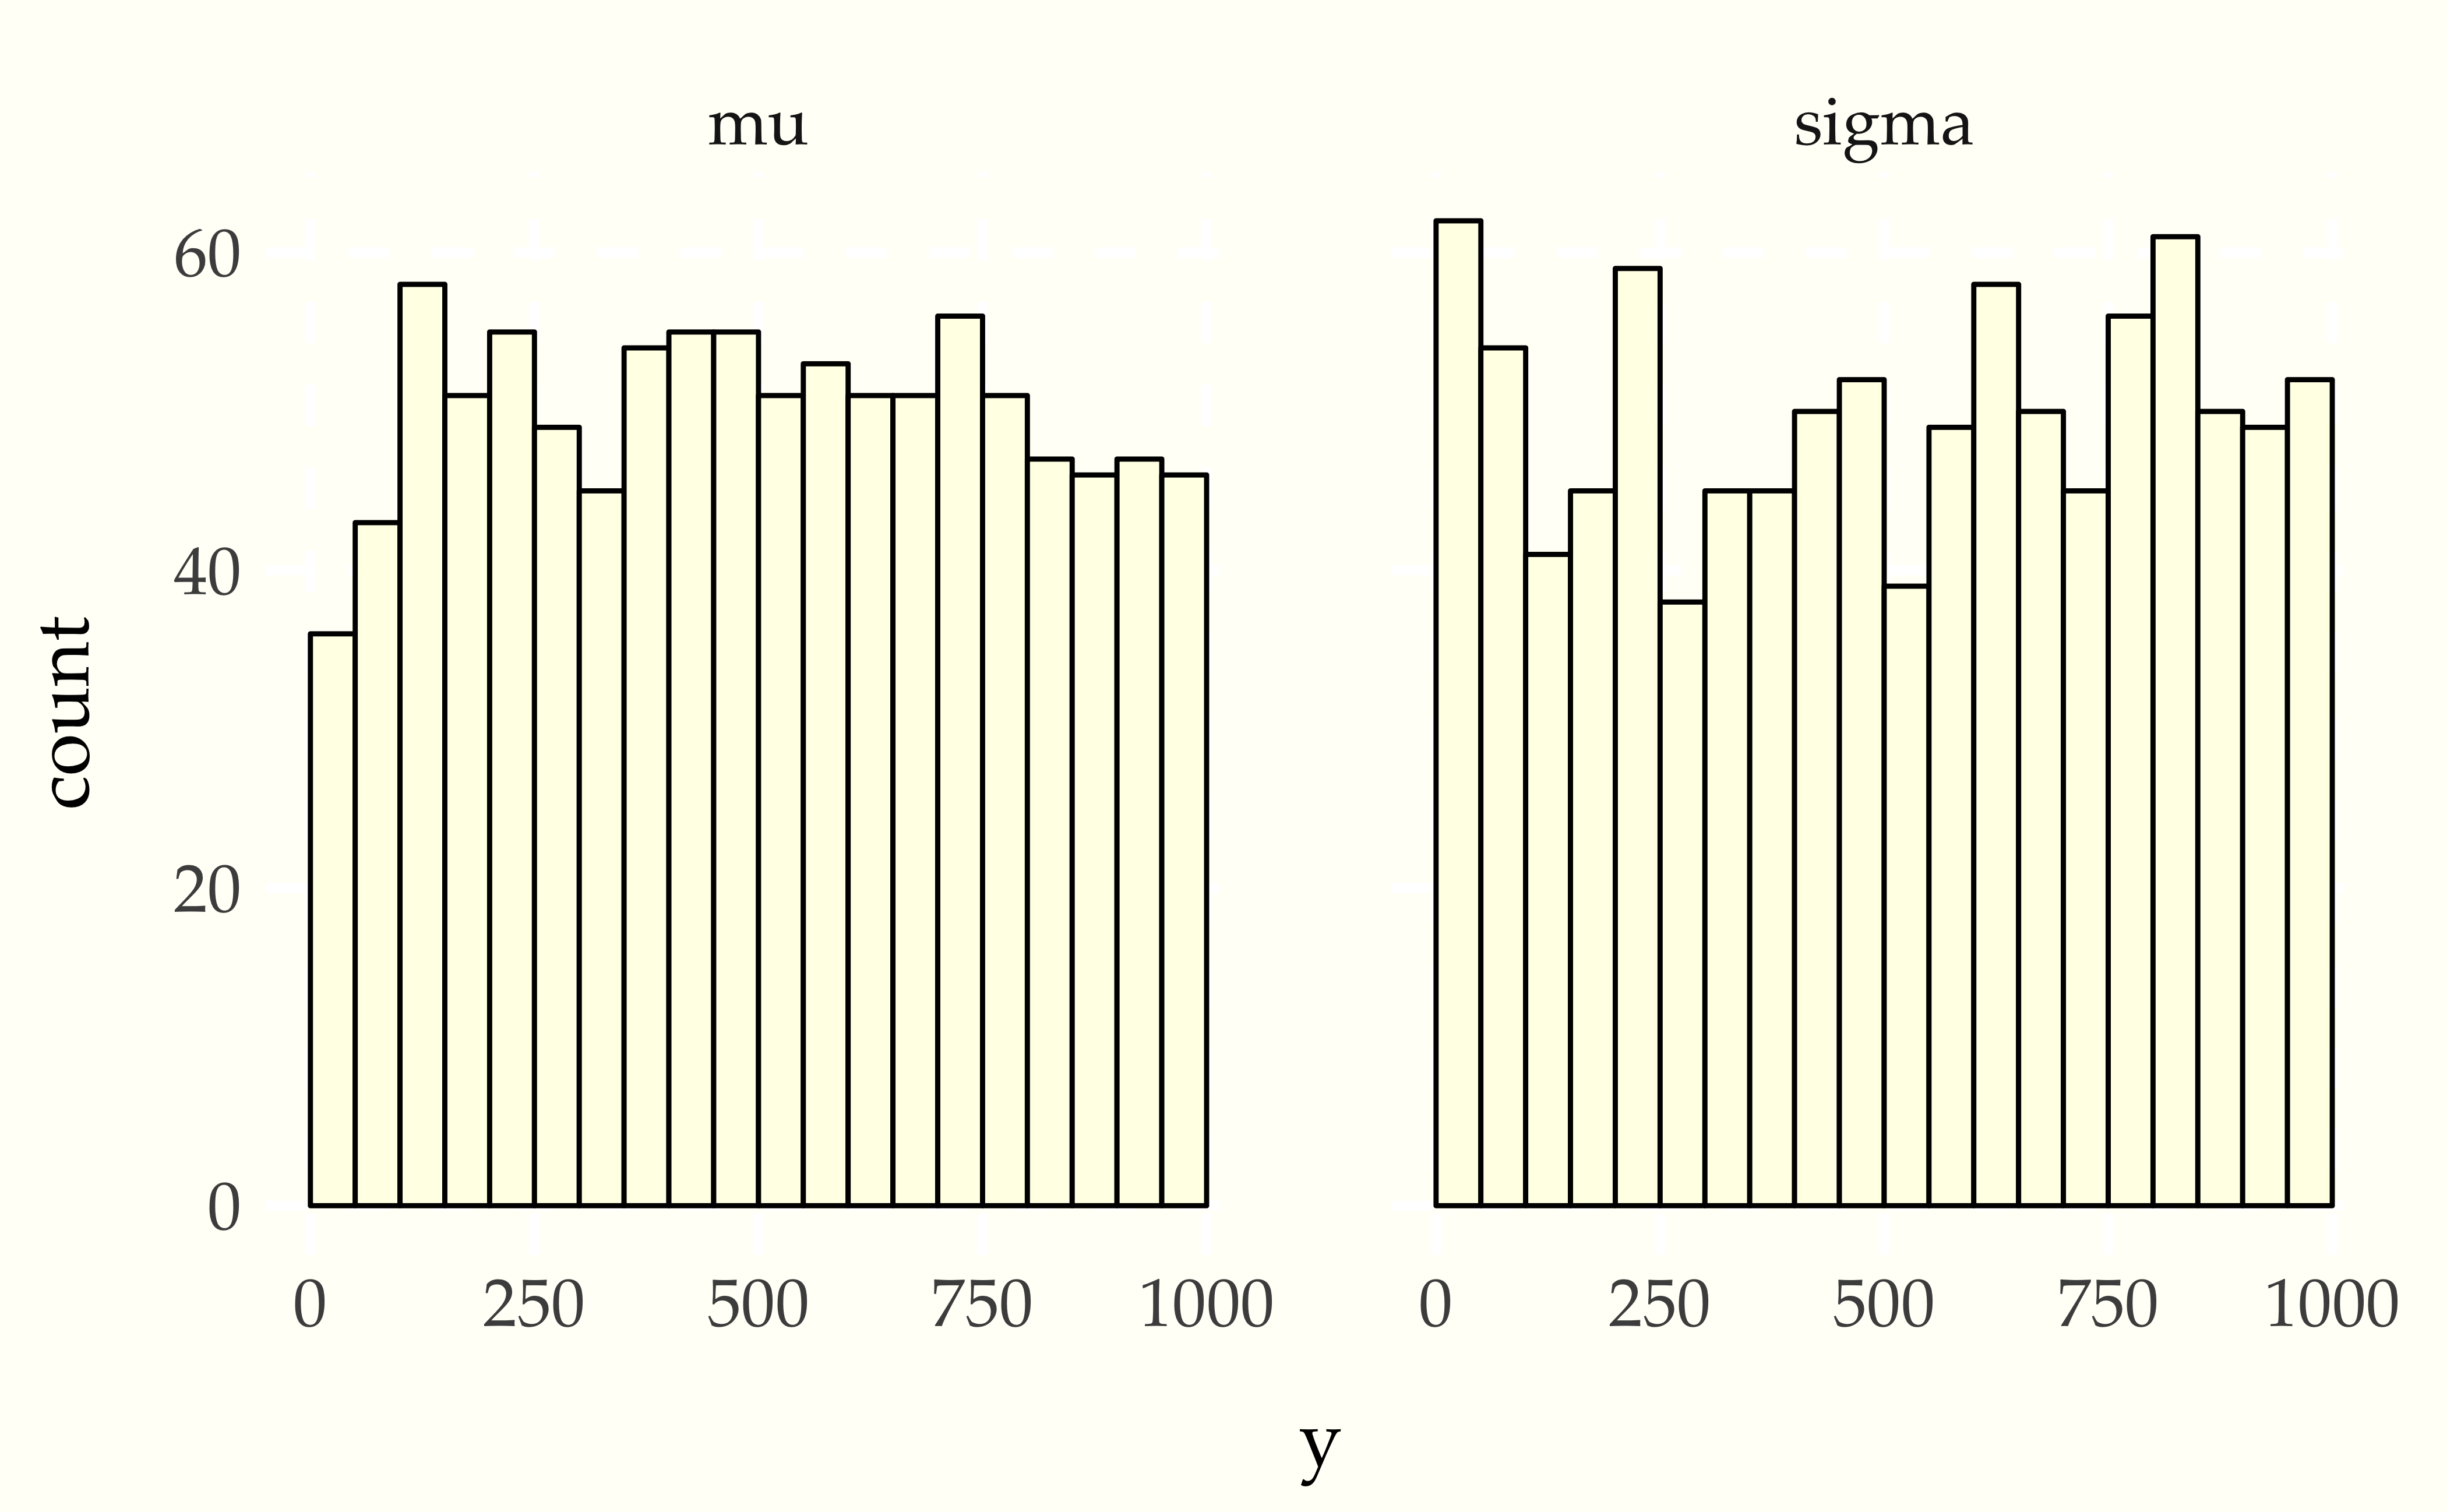
\includegraphics[width=0.7\linewidth]{./img/sbc-normal-normal} 

}

\caption{Simulation based calibration plots for location and scale  of a normal model with standard normal prior on the location  standard lognormal prior on the scale.  Both histograms appear uniform, which is consistent with inference being well calibrated.}\label{fig:unnamed-chunk-45}
\end{figure}

\hypertarget{when-things-go-wrong}{%
\subsection{When things go wrong}\label{when-things-go-wrong}}

Now consider using a Student-t data generating process with a normal model.
Compare the apparent uniformity of the well specified model with the
ill-specified situation with Student-t generative process and normal
model.

\begin{figure}

{\centering 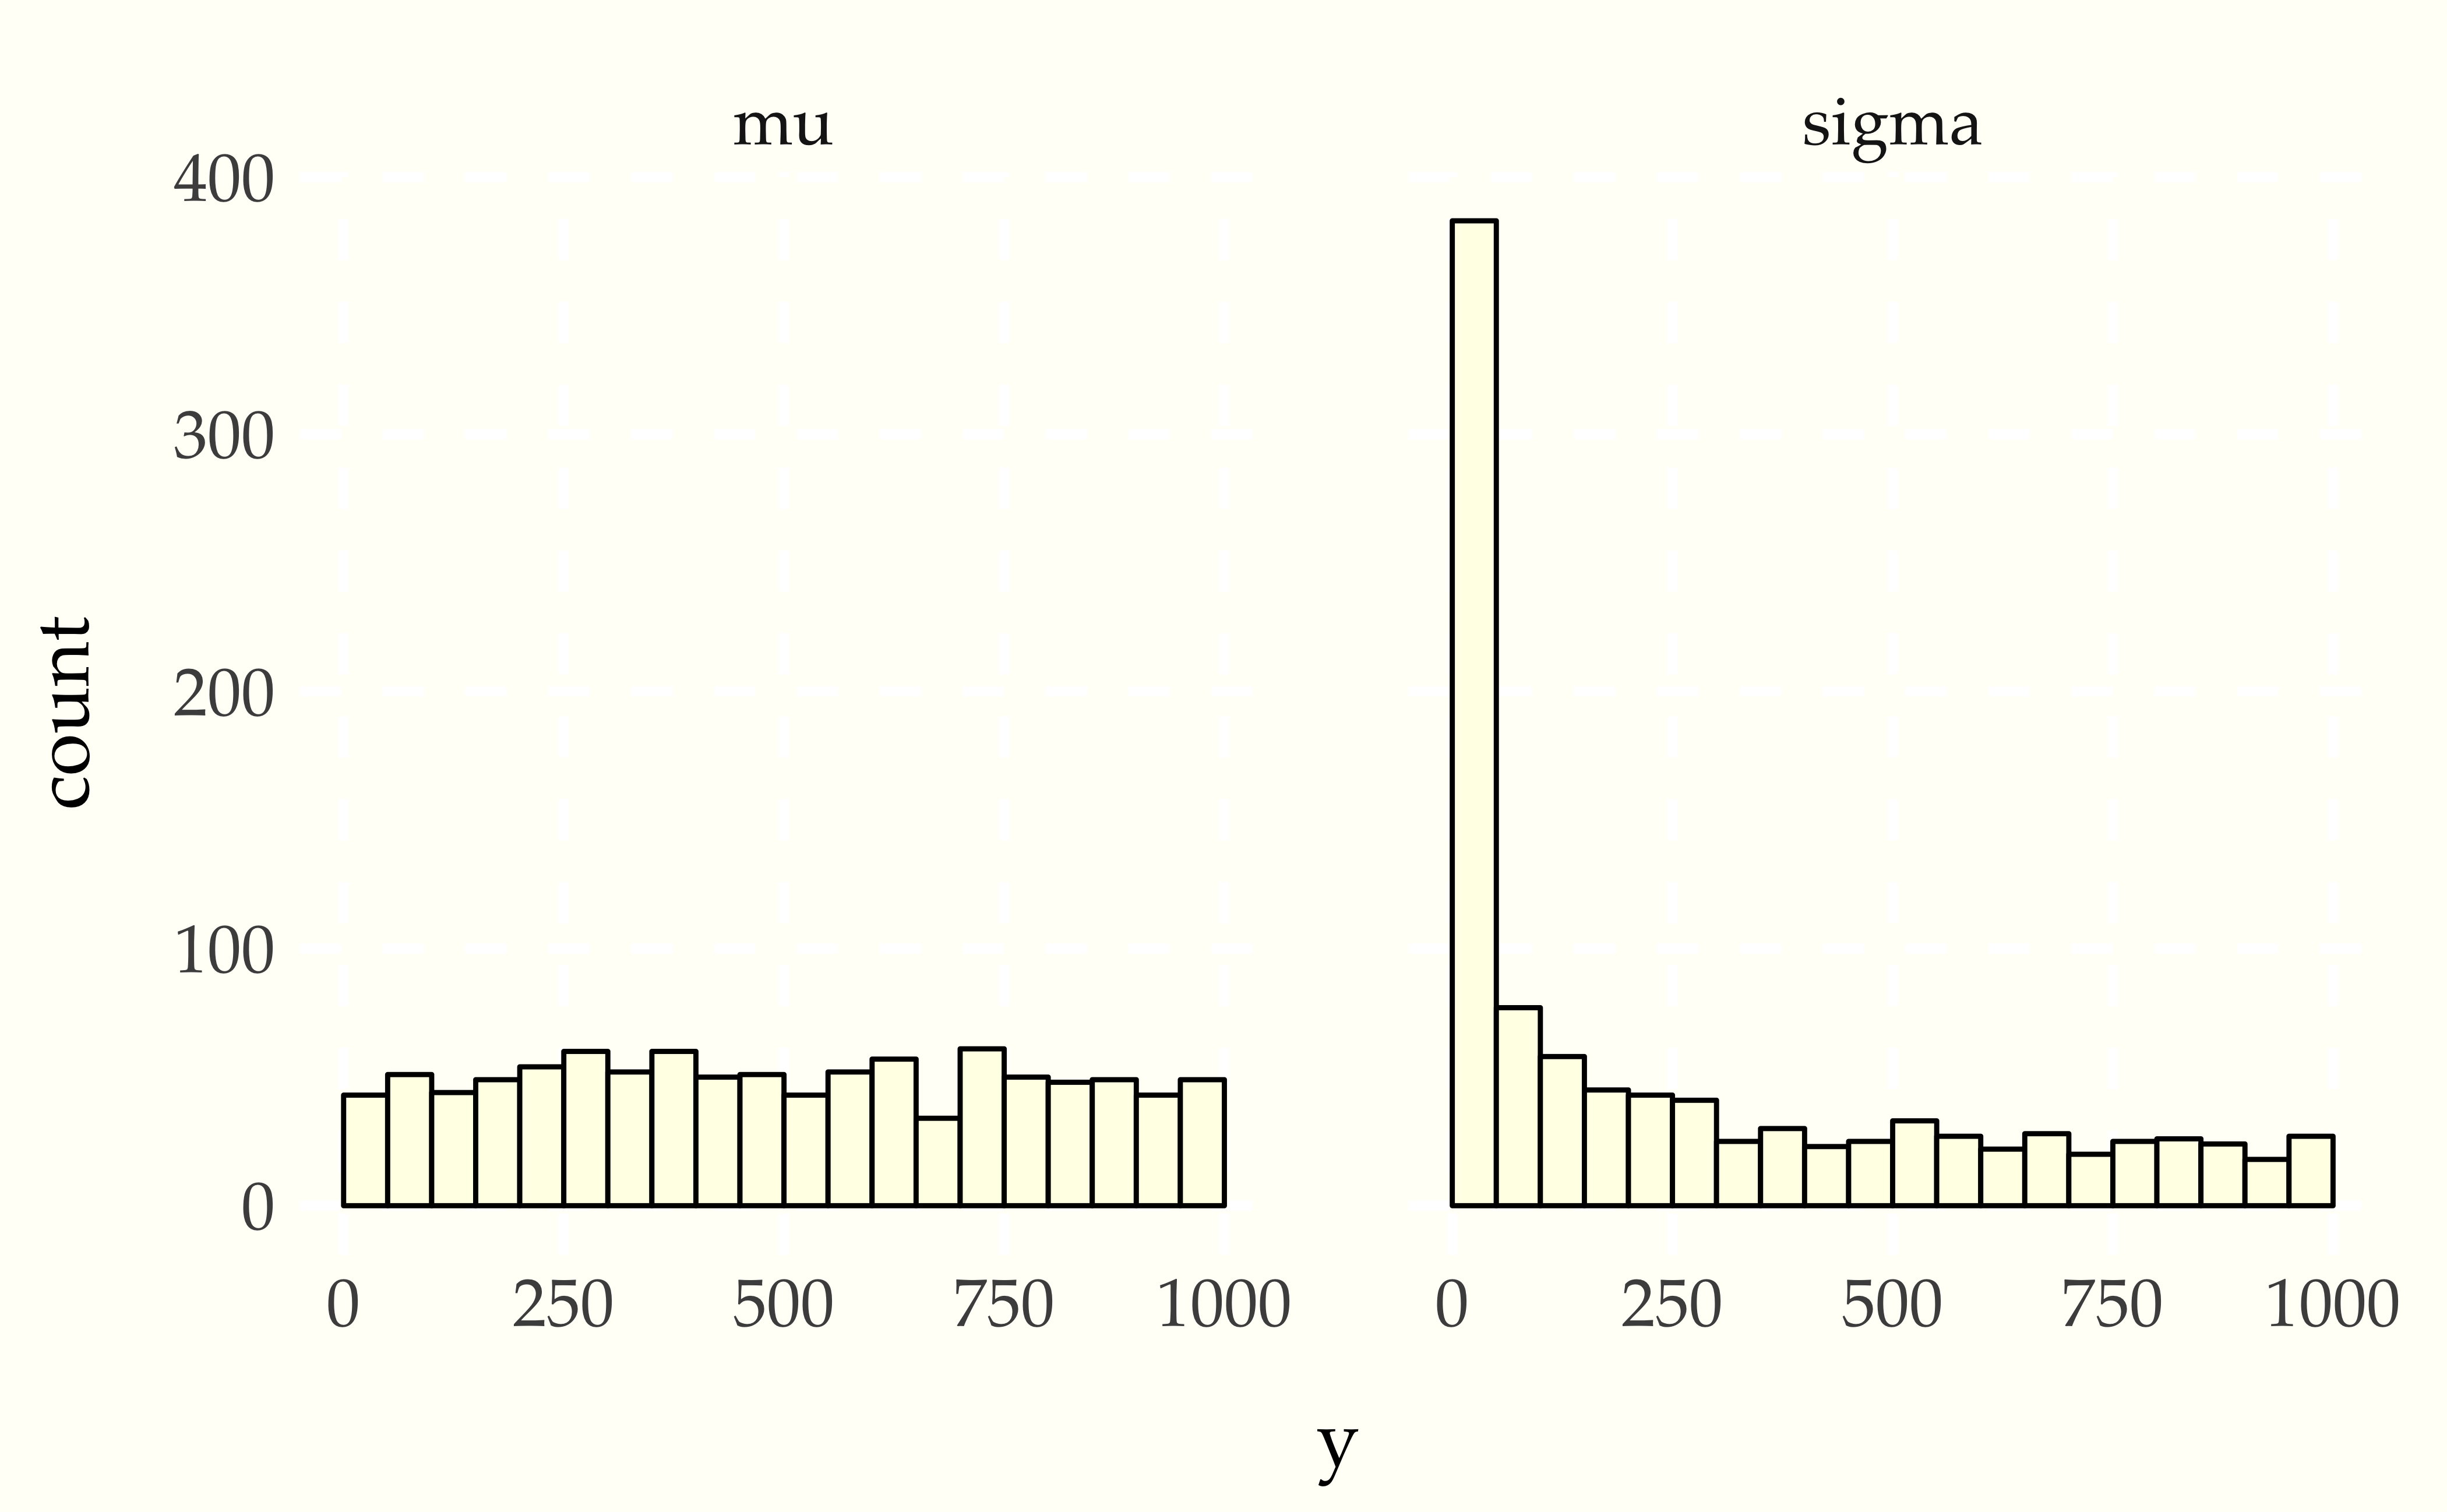
\includegraphics[width=0.7\linewidth]{./img/sbc-student-t-normal} 

}

\caption{Simulation based calibration plots for location and scale of a normal model with standard normal prior on the location standard lognormal prior on the scale with mismatched generative model using a Student-t likelihood with 4 degrees of freedom.  The mean histogram appears uniform, but the scale parameter shows simulated values much smaller than fit values, clearly signaling the lack of calibration.}\label{fig:unnamed-chunk-46}
\end{figure}

\hypertarget{when-stans-sampler-goes-wrong}{%
\subsection{When Stan's sampler goes wrong}\label{when-stans-sampler-goes-wrong}}

The example in the previous sections show hard-coded pathological
behavior. The usual application of SBC is to diagnose problems with a
sampler.

This can happen in Stan with well-specified models if the posterior
geometry is too difficult (usually due to extreme stiffness that
varies). A simple example is the eight schools problem,
the data for which consists of sample means \(y_j\) and standard
deviations \(\sigma_j\) of differences in test score after the same
intervention in \(J = 8\) different schools. Donald B. Rubin (\protect\hyperlink{ref-Rubin:1981}{1981}) applies a
hierarchical model for a meta-analysis of the results, estimating the
mean intervention effect and a varying effect for each school. With a
standard parameterization and weak priors, this model has very
challenging posterior geometry, as shown by Talts et al. (\protect\hyperlink{ref-TaltsEtAl:2018}{2018}); this
section replicates their results.

The meta-analysis model has parameters for a population mean \(\mu\) and
standard deviation \(\tau > 0\) as well as the effect \(\theta_j\) of the
treatment in each school. The model has weak normal and half-normal
priors for the population-level parameters,
\begin{eqnarray*}
\mu & \sim & \textrm{normal}(0, 5)
\\[4pt]
\tau & \sim & \textrm{normal}_{+}(0, 5).
\end{eqnarray*}
School level effects are modeled as normal given the population
parameters,
\[
\theta_j \sim \textrm{normal}(\mu, \tau).
\]
The data is modeled as in a meta-analysis, given the school effect and
sample standard deviation in the school,
\[
y_j \sim \textrm{normal}(\theta_j, \sigma_j).
\]

This model can be coded in Stan with a data-generating process that
simulates the parameters and then simulates data according to the
parameters.

\begin{Shaded}
\begin{Highlighting}[]
\KeywordTok{transformed data}\NormalTok{ \{}
  \DataTypeTok{real}\NormalTok{ mu\_sim = normal\_rng(}\DecValTok{0}\NormalTok{, }\DecValTok{5}\NormalTok{);}
  \DataTypeTok{real}\NormalTok{ tau\_sim = fabs(normal\_rng(}\DecValTok{0}\NormalTok{, }\DecValTok{5}\NormalTok{));}
  \DataTypeTok{int}\NormalTok{\textless{}}\KeywordTok{lower}\NormalTok{=}\DecValTok{0}\NormalTok{\textgreater{} J = }\DecValTok{8}\NormalTok{;}
  \DataTypeTok{array}\NormalTok{[J] }\DataTypeTok{real}\NormalTok{ theta\_sim = normal\_rng(rep\_vector(mu\_sim, J), tau\_sim);}
  \DataTypeTok{array}\NormalTok{[J] }\DataTypeTok{real}\NormalTok{\textless{}}\KeywordTok{lower}\NormalTok{=}\DecValTok{0}\NormalTok{\textgreater{} sigma = fabs(normal\_rng(rep\_vector(}\DecValTok{0}\NormalTok{, J), }\DecValTok{5}\NormalTok{));}
  \DataTypeTok{array}\NormalTok{[J] }\DataTypeTok{real}\NormalTok{ y = normal\_rng(theta\_sim, sigma);}
\NormalTok{\}}
\KeywordTok{parameters}\NormalTok{ \{}
  \DataTypeTok{real}\NormalTok{ mu;}
  \DataTypeTok{real}\NormalTok{\textless{}}\KeywordTok{lower}\NormalTok{=}\DecValTok{0}\NormalTok{\textgreater{} tau;}
  \DataTypeTok{array}\NormalTok{[J] }\DataTypeTok{real}\NormalTok{ theta;}
\NormalTok{\}}
\KeywordTok{model}\NormalTok{ \{}
\NormalTok{  tau \textasciitilde{} normal(}\DecValTok{0}\NormalTok{, }\DecValTok{5}\NormalTok{);}
\NormalTok{  mu \textasciitilde{} normal(}\DecValTok{0}\NormalTok{, }\DecValTok{5}\NormalTok{);}
\NormalTok{  theta \textasciitilde{} normal(mu, tau);}
\NormalTok{  y \textasciitilde{} normal(theta, sigma);}
\NormalTok{\}}
\KeywordTok{generated quantities}\NormalTok{ \{}
  \DataTypeTok{int}\NormalTok{\textless{}}\KeywordTok{lower}\NormalTok{=}\DecValTok{0}\NormalTok{, }\KeywordTok{upper}\NormalTok{=}\DecValTok{1}\NormalTok{\textgreater{} mu\_lt\_sim = mu \textless{} mu\_sim;}
  \DataTypeTok{int}\NormalTok{\textless{}}\KeywordTok{lower}\NormalTok{=}\DecValTok{0}\NormalTok{, }\KeywordTok{upper}\NormalTok{=}\DecValTok{1}\NormalTok{\textgreater{} tau\_lt\_sim = tau \textless{} tau\_sim;}
  \DataTypeTok{int}\NormalTok{\textless{}}\KeywordTok{lower}\NormalTok{=}\DecValTok{0}\NormalTok{, }\KeywordTok{upper}\NormalTok{=}\DecValTok{1}\NormalTok{\textgreater{} theta1\_lt\_sim = theta[}\DecValTok{1}\NormalTok{] \textless{} theta\_sim[}\DecValTok{1}\NormalTok{];}
\NormalTok{\}}
\end{Highlighting}
\end{Shaded}

As usual for simulation-based calibration, the transformed data
encodes the data-generating process using random number generators.
Here, the population parameters \(\mu\) and \(\tau\) are first simulated,
then the school-level effects \(\theta\), and then finally the observed
data \(\sigma_j\) and \(y_j.\) The parameters and model are a direct
encoding of the mathematical presentation using vectorized sampling
statements. The generated quantities block includes indicators for
parameter comparisons, saving only \(\theta_1\) because the schools are
exchangeable in the simulation.

When fitting the model in Stan, multiple warning messages are
provided that the sampler has diverged. The divergence warnings are
in Stan's sampler precisely to diagnose the sampler's inability
to follow the curvature in the posterior and provide independent
confirmation that Stan's sampler cannot fit this model as specified.

SBC also diagnoses the problem. Here's the rank plots for running \(N = 200\) simulations with 1000 warmup iterations and \(M = 999\) draws per
simulation used to compute the ranks.

\begin{figure}

{\centering 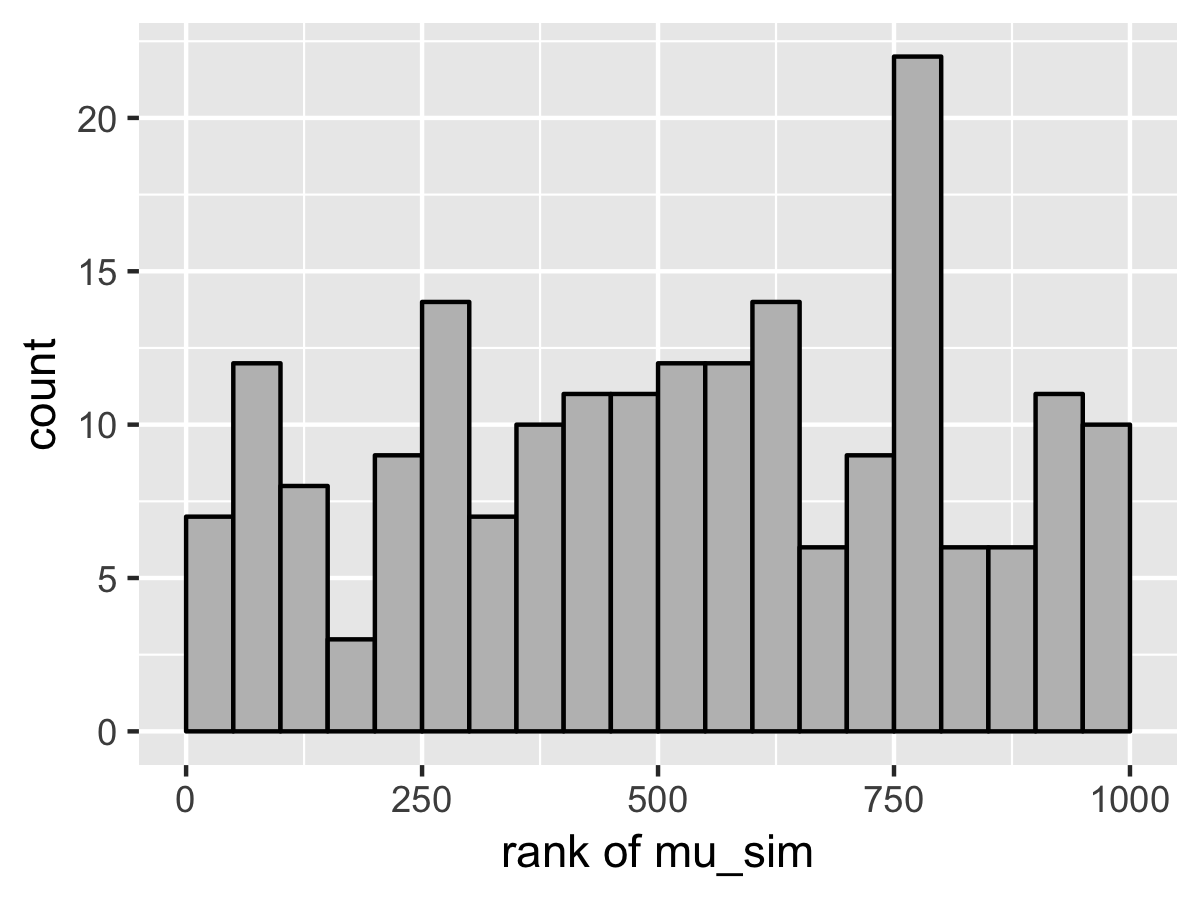
\includegraphics[width=0.3\linewidth]{./img/sbc-ctr-8-schools-mu} 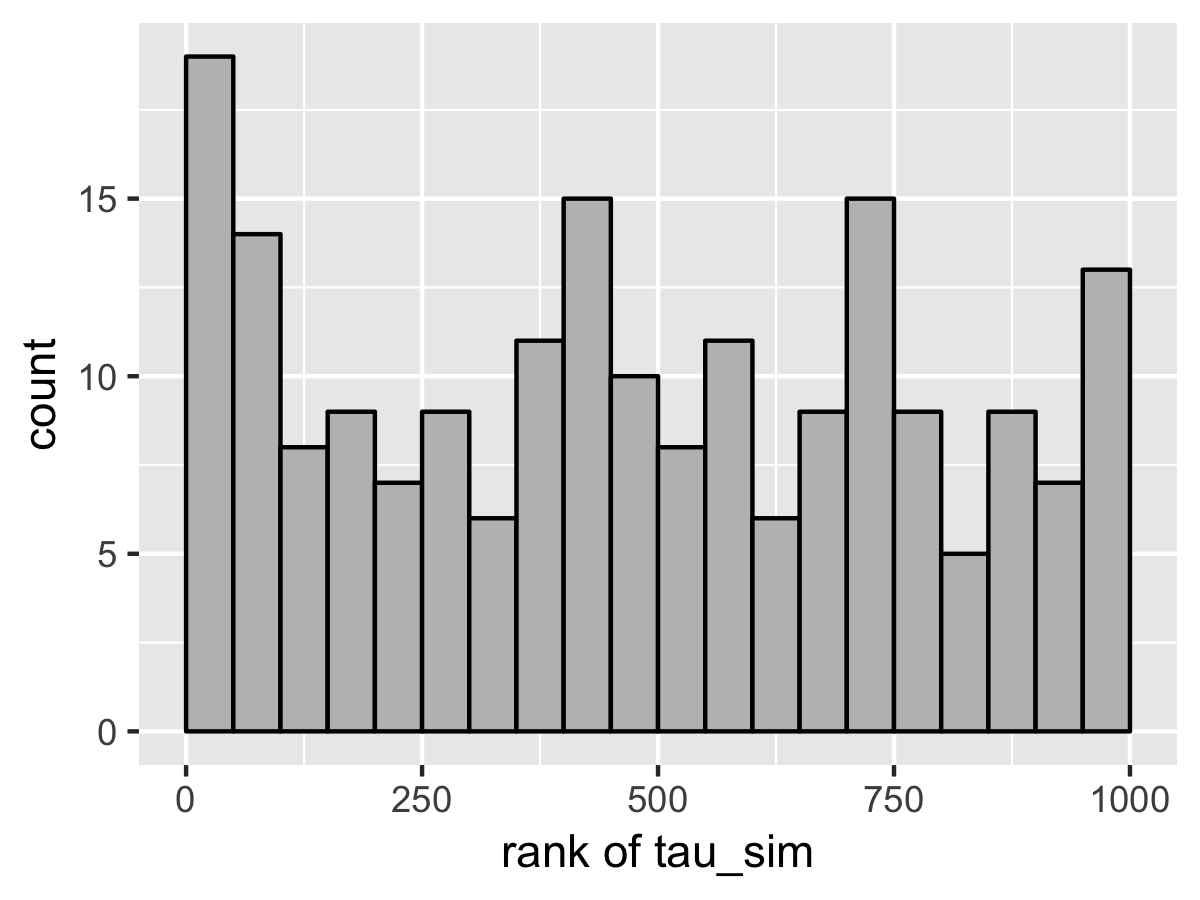
\includegraphics[width=0.3\linewidth]{./img/sbc-ctr-8-schools-tau} 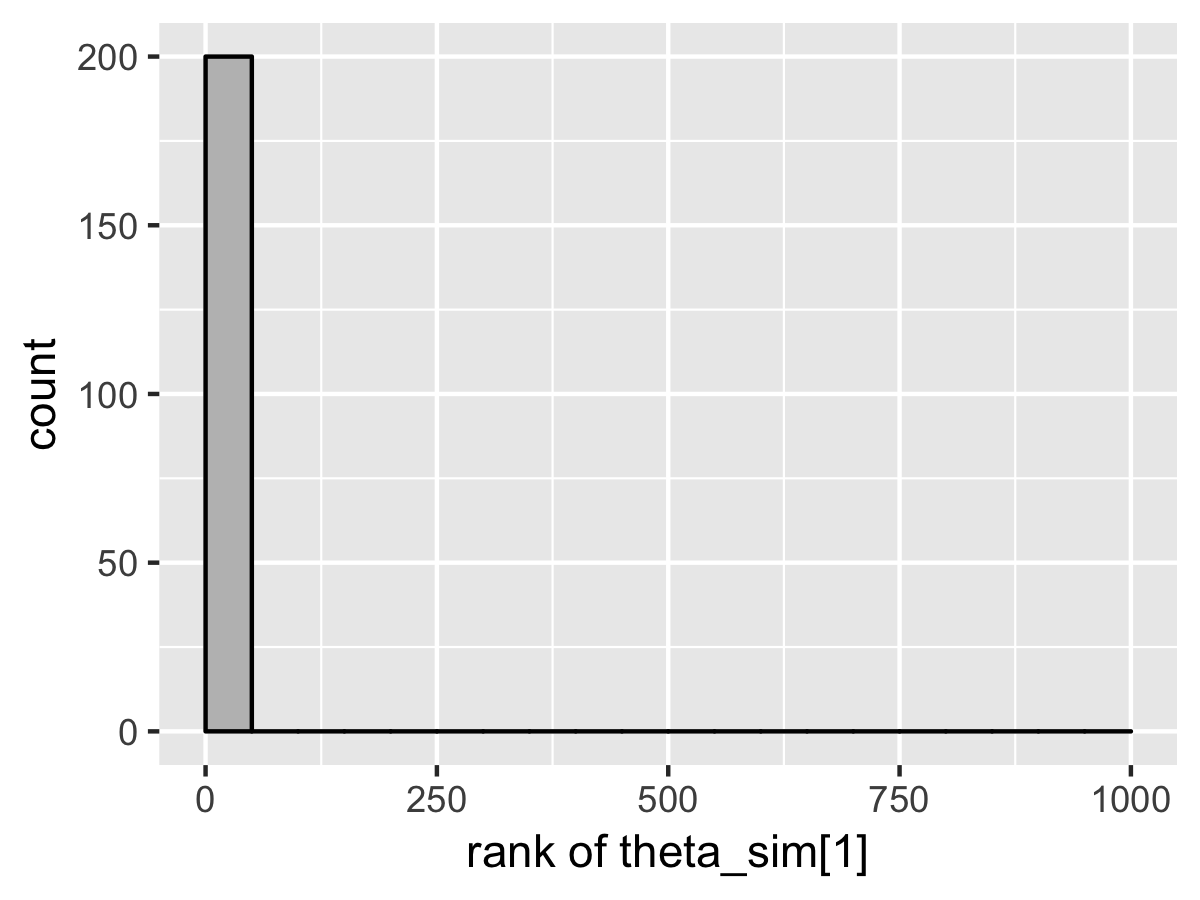
\includegraphics[width=0.3\linewidth]{./img/sbc-ctr-8-schools-theta1} 

}

\caption{Simulation based calibration plots for the eight-schools model with  centered parameterization in Stan.  The geometry is too difficult for the NUTS sampler to handle, as indicated by the plot for theta[1].}\label{fig:unnamed-chunk-47}
\end{figure}

Although the population mean and standard deviation \(\mu\) and \(\tau\)
appear well calibrated, \(\theta_1\) tells a very different story. The
simulated values are much smaller than the values fit from the data.
This is because Stan's no-U-turn sampler is unable to sample with the
model formulated in the centered parameterization---the posterior
geometry has regions of extremely high curvature as \(\tau\) approaches
zero and the \(\theta_j\) become highly constrained. The \protect\hyperlink{change-of-variables.chapter}{chapter on
reparameterization} explains how to
remedy this problem and fit this kind of hierarchical model with Stan.

\hypertarget{ppcs.chapter}{%
\chapter{Posterior and Prior Predictive Checks}\label{ppcs.chapter}}

Posterior predictive checks are a way of measuring whether a model
does a good job of capturing relevant aspects of the data, such as
means, standard deviations, and quantiles (\protect\hyperlink{ref-Rubin:1984}{Donald B. Rubin 1984}; \protect\hyperlink{ref-GelmanEtAl:1996}{Andrew Gelman, Meng, and Stern 1996}). Posterior predictive checking works by simulating
new replicated data sets based on the fitted model parameters and then
comparing statistics applied to the replicated data set with the same
statistic applied to the original data set.

Prior predictive checks evaluate the prior the same way.
Specifically, they evaluate what data sets would be consistent with
the prior. They will not be calibrated with actual data, but extreme
values help diagnose priors that are either too strong, too weak,
poorly shaped, or poorly located.

Prior and posterior predictive checks are two cases of the general
concept of predictive checks, just conditioning on different things
(no data and the observed data, respectively). For hierarchical
models, there are intermediate versions, as discussed in the section
on \protect\hyperlink{mixed-replication}{hierarchical models and mixed replication}.

\hypertarget{simulating-from-the-posterior-predictive-distribution}{%
\section{Simulating from the posterior predictive distribution}\label{simulating-from-the-posterior-predictive-distribution}}

The posterior predictive distribution is the distribution over new
observations given previous observations. It's predictive in the
sense that it's predicting behavior on new data that is not part of
the training set. It's posterior in that everything is conditioned on
observed data \(y\).

The posterior predictive distribution for replications
\(y^{\textrm{rep}}\) of the original data set \(y\) given model parameters
\(\theta\) is defined by
\[
p(y^{\textrm{rep}} \mid y)
= \int p(y^{\textrm{rep}} \mid \theta)
       \cdot p(\theta \mid y) \, \textrm{d}\theta.
\]

As with other posterior predictive quantities, generating a replicated
data set \(y^{\textrm{rep}}\) from the posterior predictive distribution is
straightforward using the generated quantities block. Consider a simple regression
model with parameters \(\theta = (\alpha, \beta, \sigma).\)

\begin{Shaded}
\begin{Highlighting}[]
\KeywordTok{data}\NormalTok{ \{}
  \DataTypeTok{int}\NormalTok{\textless{}}\KeywordTok{lower}\NormalTok{=}\DecValTok{0}\NormalTok{\textgreater{} N;}
  \DataTypeTok{vector}\NormalTok{[N] x;}
  \DataTypeTok{vector}\NormalTok{[N] y;}
\NormalTok{\}}
\KeywordTok{parameters}\NormalTok{ \{}
  \DataTypeTok{real}\NormalTok{ alpha;}
  \DataTypeTok{real}\NormalTok{ beta;}
  \DataTypeTok{real}\NormalTok{\textless{}}\KeywordTok{lower}\NormalTok{=}\DecValTok{0}\NormalTok{\textgreater{} sigma;}
\NormalTok{\}}
\KeywordTok{model}\NormalTok{ \{}
\NormalTok{  alpha \textasciitilde{} normal(}\DecValTok{0}\NormalTok{, }\DecValTok{2}\NormalTok{);}
\NormalTok{  beta \textasciitilde{} normal(}\DecValTok{0}\NormalTok{, }\DecValTok{1}\NormalTok{);}
\NormalTok{  sigma \textasciitilde{} normal(}\DecValTok{0}\NormalTok{, }\DecValTok{1}\NormalTok{);}
\NormalTok{  y \textasciitilde{} normal(alpha + beta * x, sigma);}
\NormalTok{\}}
\end{Highlighting}
\end{Shaded}

To generate a replicated data set \texttt{y\_rep} for this simple model, the
following generated quantities block suffices.

\begin{Shaded}
\begin{Highlighting}[]
\KeywordTok{generated quantities}\NormalTok{ \{}
  \DataTypeTok{array}\NormalTok{[N] }\DataTypeTok{real}\NormalTok{ y\_rep = normal\_rng(alpha + beta * x, sigma);}
\NormalTok{\}}
\end{Highlighting}
\end{Shaded}

The vectorized form of the normal random
number generator is used with the original predictors \texttt{x} and the
model parameters \texttt{alpha,\ beta}, and \texttt{sigma.}
The replicated data variable \texttt{y\_rep} is declared to be the same size
as the original data \texttt{y}, but instead of a vector type, it is
declared to be an array of reals to match
the return type of the function \texttt{normal\_rng}.
Because the vector and real array types have the same dimensions and layout,
they can be plotted against one another and otherwise compared during
downstream processing.

The posterior predictive
sampling for posterior predictive checks is different from usual
posterior predictive sampling discussed in \protect\hyperlink{posterior-prediction.chapter}{the chapter on posterior
predictions} in that the original
predictors \(x\) are used. That is, the posterior predictions are for
the original data.

\hypertarget{plotting-multiples}{%
\section{Plotting multiples}\label{plotting-multiples}}

A standard posterior predictive check would plot a histogram of each
replicated data set along with the original data set and compare them
by eye. For this purpose, only a few replications are needed. These
should be taken by thinning a larger set of replications down to the
size needed to ensure rough independence of the replications.

Here's a complete example where the model is a simple Poisson with
a weakly informative exponential prior with a mean of 10 and
standard deviation of 10.

\begin{Shaded}
\begin{Highlighting}[]
\KeywordTok{data}\NormalTok{ \{}
  \DataTypeTok{int}\NormalTok{\textless{}}\KeywordTok{lower}\NormalTok{=}\DecValTok{0}\NormalTok{\textgreater{} N;}
  \DataTypeTok{array}\NormalTok{[N] }\DataTypeTok{int}\NormalTok{\textless{}}\KeywordTok{lower}\NormalTok{=}\DecValTok{0}\NormalTok{\textgreater{} y;}
\NormalTok{\}}
\KeywordTok{transformed data}\NormalTok{ \{}
  \DataTypeTok{real}\NormalTok{\textless{}}\KeywordTok{lower}\NormalTok{=}\DecValTok{0}\NormalTok{\textgreater{} mean\_y = mean(to\_vector(y));}
  \DataTypeTok{real}\NormalTok{\textless{}}\KeywordTok{lower}\NormalTok{=}\DecValTok{0}\NormalTok{\textgreater{} sd\_y = sd(to\_vector(y));}
\NormalTok{\}}
\KeywordTok{parameters}\NormalTok{ \{}
  \DataTypeTok{real}\NormalTok{\textless{}}\KeywordTok{lower}\NormalTok{=}\DecValTok{0}\NormalTok{\textgreater{} lambda;}
\NormalTok{\}}
\KeywordTok{model}\NormalTok{ \{}
\NormalTok{  y \textasciitilde{} poisson(lambda);}
\NormalTok{  lambda \textasciitilde{} exponential(}\FloatTok{0.2}\NormalTok{);}
\NormalTok{\}}
\KeywordTok{generated quantities}\NormalTok{ \{}
  \DataTypeTok{array}\NormalTok{[N] }\DataTypeTok{int}\NormalTok{\textless{}}\KeywordTok{lower}\NormalTok{=}\DecValTok{0}\NormalTok{\textgreater{} y\_rep = poisson\_rng(rep\_array(lambda, N));}
  \DataTypeTok{real}\NormalTok{\textless{}}\KeywordTok{lower}\NormalTok{=}\DecValTok{0}\NormalTok{\textgreater{} mean\_y\_rep = mean(to\_vector(y\_rep));}
  \DataTypeTok{real}\NormalTok{\textless{}}\KeywordTok{lower}\NormalTok{=}\DecValTok{0}\NormalTok{\textgreater{} sd\_y\_rep = sd(to\_vector(y\_rep));}
  \DataTypeTok{int}\NormalTok{\textless{}}\KeywordTok{lower}\NormalTok{=}\DecValTok{0}\NormalTok{, }\KeywordTok{upper}\NormalTok{=}\DecValTok{1}\NormalTok{\textgreater{} mean\_gte = (mean\_y\_rep \textgreater{}= mean\_y);}
  \DataTypeTok{int}\NormalTok{\textless{}}\KeywordTok{lower}\NormalTok{=}\DecValTok{0}\NormalTok{, }\KeywordTok{upper}\NormalTok{=}\DecValTok{1}\NormalTok{\textgreater{} sd\_gte = (sd\_y\_rep \textgreater{}= sd\_y);}
\NormalTok{\}}
\end{Highlighting}
\end{Shaded}

The generated quantities block creates a variable \texttt{y\_rep} for the
replicated data, variables \texttt{mean\_y\_rep} and \texttt{sd\_y\_rep} for the
statistics of the replicated data, and indicator variables
\texttt{mean\_gte} and \texttt{sd\_gte} for whether the replicated statistic
is greater than or equal to the statistic applied to the original
data.

Now consider generating data \(y \sim \textrm{Poisson}(5)\). The
resulting small multiples plot shows the original data plotted in the
upper left and eight different posterior replications plotted in the
remaining boxes.

\begin{figure}

{\centering 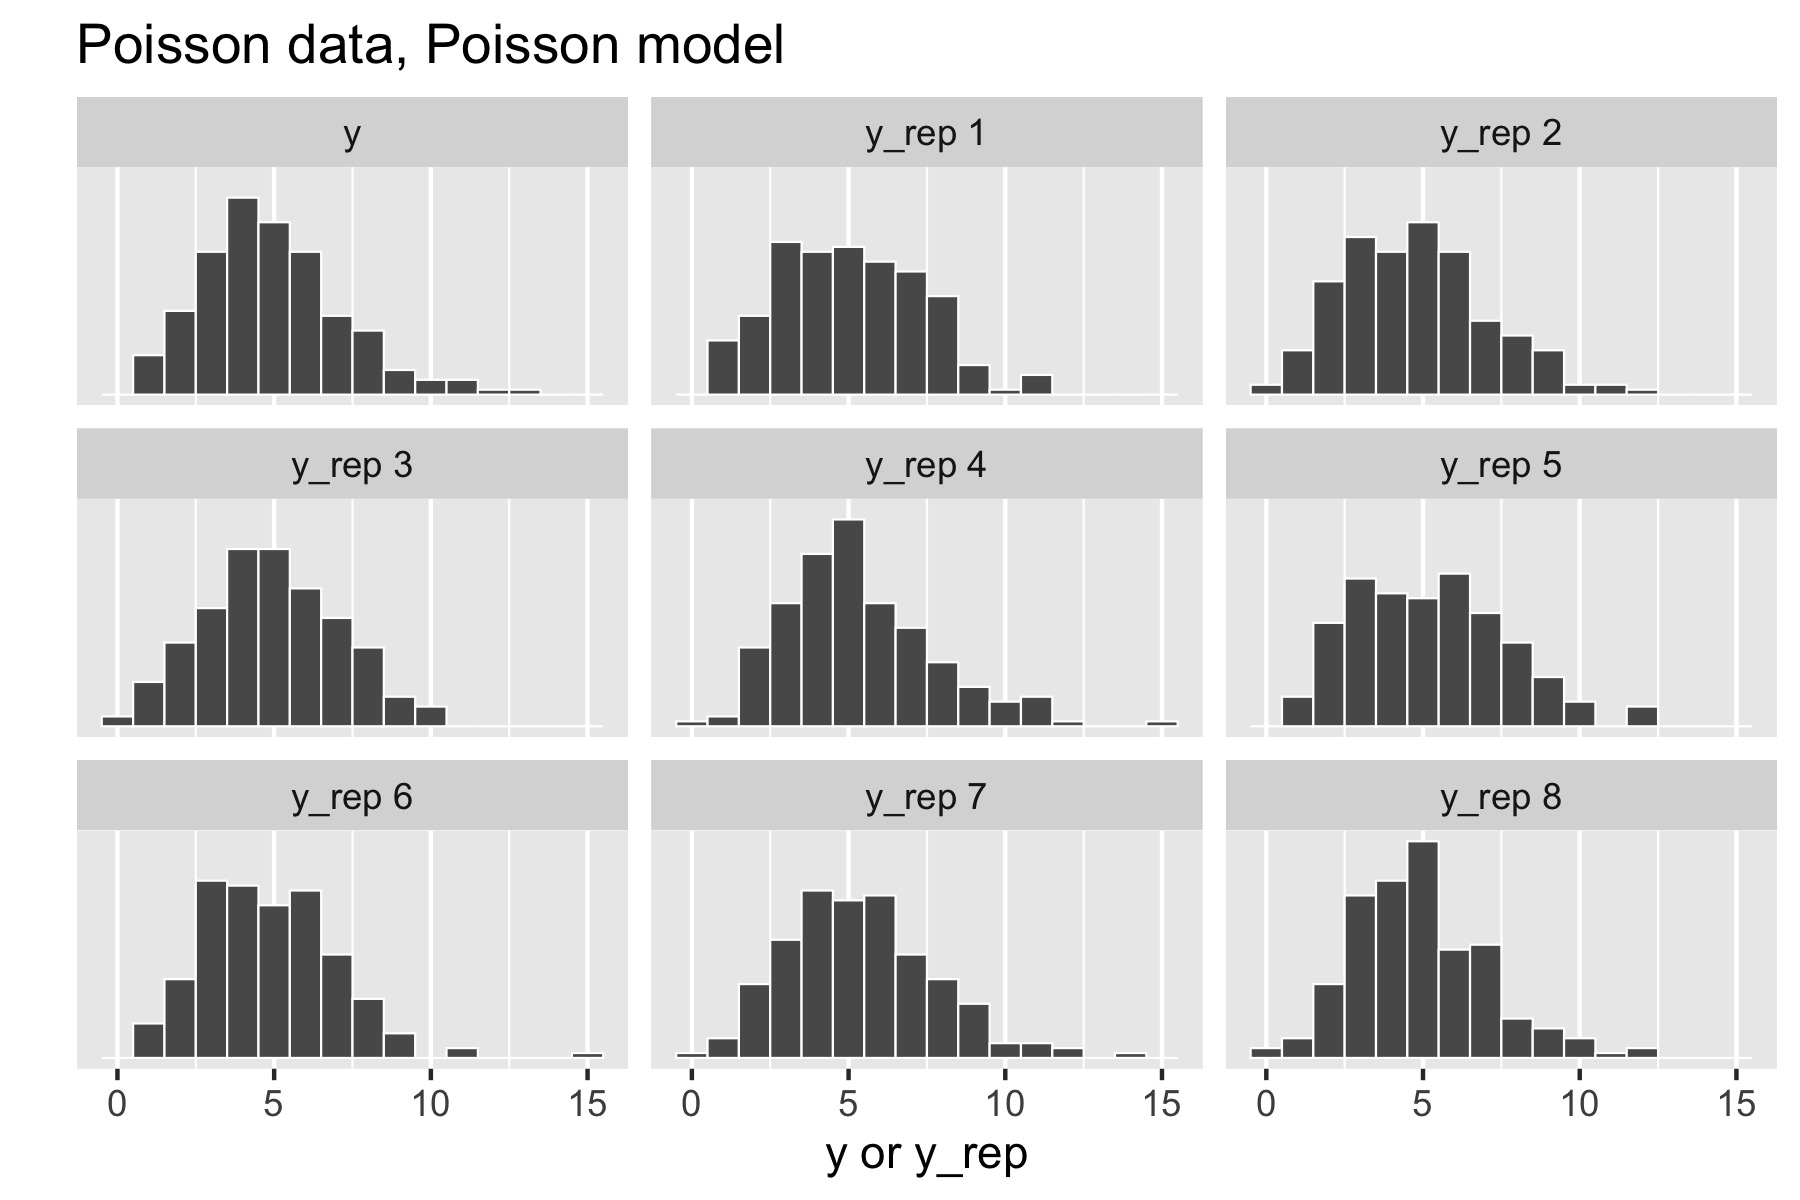
\includegraphics[width=0.7\linewidth]{./img/ppc-pois-pois} 

}

\caption{Posterior predictive checks for Poisson data generating process and Poisson model.}\label{fig:unnamed-chunk-49}
\end{figure}

With a Poisson data-generating process and Poisson model, the
posterior replications look similar to the original data. If it were
easy to pick the original data out of the lineup, there would be a
problem.

Now consider generating over-dispersed data \(y \sim \textrm{negative-binomial2}(5, 1).\) This has the same mean as
\(\textrm{Poisson}(5)\), namely \(5\), but a standard deviation of
\(\sqrt{5 + 5^2 /1} \approx 5.5.\) There is no way to fit this data with
the Poisson model, because a variable distributed as
\(\textrm{Poisson}(\lambda)\) has mean \(\lambda\) and standard deviation
\(\sqrt{\lambda},\) which is \(\sqrt{5}\) for \(\textrm{Poisson}(5).\)
Here's the resulting small multiples plot, again with original data in
the upper left.

\begin{figure}

{\centering 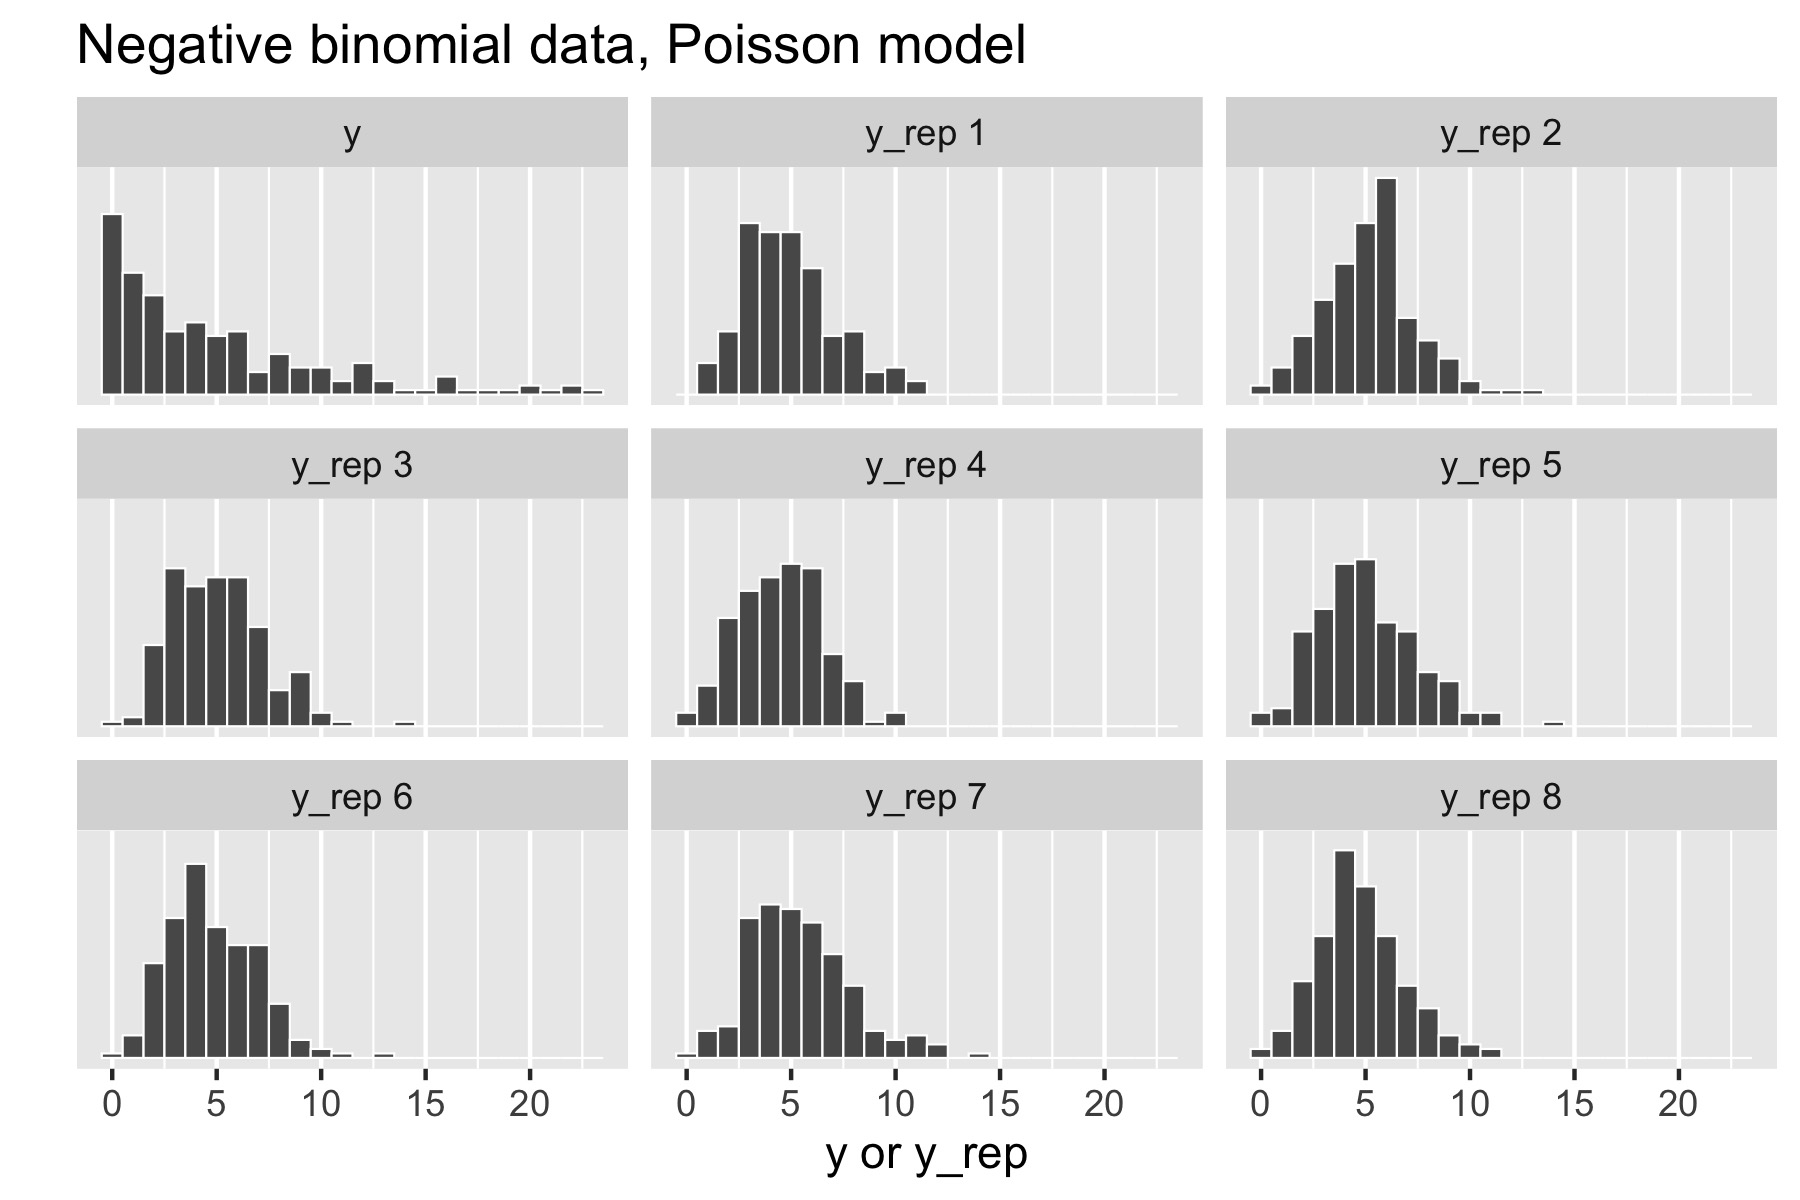
\includegraphics[width=0.7\linewidth]{./img/ppc-nb-pois} 

}

\caption{Posterior predictive checks for negative binomial data generating process and Poisson model.}\label{fig:unnamed-chunk-50}
\end{figure}

This time, the original data stands out in stark contrast to the
replicated data sets, all of which are clearly more symmetric and
lower variance than the original data. That is, the model's not
appropriately capturing the variance of the data.

\hypertarget{posterior-p-values}{%
\section{Posterior ``p-values'\,'}\label{posterior-p-values}}

If a model captures the data well, summary statistics such as
sample mean and standard deviation, should have similar values in
the original and replicated data sets. This can be tested
by means of a p-value-like statistic, which here is just the probability the
test statistic \(s(\cdot)\) in a replicated data set exceeds that in
the original data,
\[
\textrm{Pr}\left[ s(y^{\textrm{rep}}) \geq s(y) \mid y \right]
=
\int
\textrm{I}\left( s(y^{\textrm{rep}}) \geq s(y) \mid y \right)
\cdot p\left( y^{\textrm{rep}} \mid y \right)
\, \textrm{d}{y^{\textrm{rep}}}.
\]
It is important to note that``p-values'\,' is in quotes because these
statistics are not classically calibrated, and thus will not in
general have a uniform distribution even when the model is well
specified (\protect\hyperlink{ref-BayarriBerger:2000}{Bayarri and Berger 2000}).

Nevertheless, values of this statistic very close to zero or
one are cause for concern that the model is not fitting the data well.
Unlike a visual test, this p-value-like test is easily automated for
bulk model fitting.

To calculate event probabilities in Stan, it suffices to define
indicator variables that take on value 1 if the event occurs and
0 if it does not. The posterior mean is then the event probability.
For efficiency, indicator variables are defined in the
generated quantities block.

\begin{Shaded}
\begin{Highlighting}[]
\KeywordTok{generated quantities}\NormalTok{ \{}
  \DataTypeTok{int}\NormalTok{\textless{}}\KeywordTok{lower}\NormalTok{=}\DecValTok{0}\NormalTok{, }\KeywordTok{upper}\NormalTok{=}\DecValTok{1}\NormalTok{\textgreater{} mean\_gt;}
  \DataTypeTok{int}\NormalTok{\textless{}}\KeywordTok{lower}\NormalTok{=}\DecValTok{0}\NormalTok{, }\KeywordTok{upper}\NormalTok{=}\DecValTok{1}\NormalTok{\textgreater{} sd\_gt;}
\NormalTok{  \{}
    \DataTypeTok{array}\NormalTok{[N] }\DataTypeTok{real}\NormalTok{ y\_rep = normal\_rng(alpha + beta * x, sigma);}
\NormalTok{    mean\_gt = mean(y\_rep) \textgreater{} mean(y);}
\NormalTok{    sd\_gt = sd(y\_rep) \textgreater{} sd(y);}
\NormalTok{  \}}
\NormalTok{\}}
\end{Highlighting}
\end{Shaded}

The indicator variable \texttt{mean\_gt} will have value 1 if the mean of the
simulated data \texttt{y\_rep} is greater than or equal to the mean of he
original data \texttt{y}. Because the values of \texttt{y\_rep} are not needed for
the posterior predictive checks, the program saves output space by
using a local variable for \texttt{y\_rep}. The statistics \texttt{mean(u)} and
\texttt{sd(y)} could also be computed in the transformed data block and
saved.

For the example in the previous section, where over-dispersed
data generated by a negative binomial distribution was fit with a
simple Poisson model, the following plot illustrates the posterior
p-value calculation for the mean statistic.

\begin{figure}

{\centering 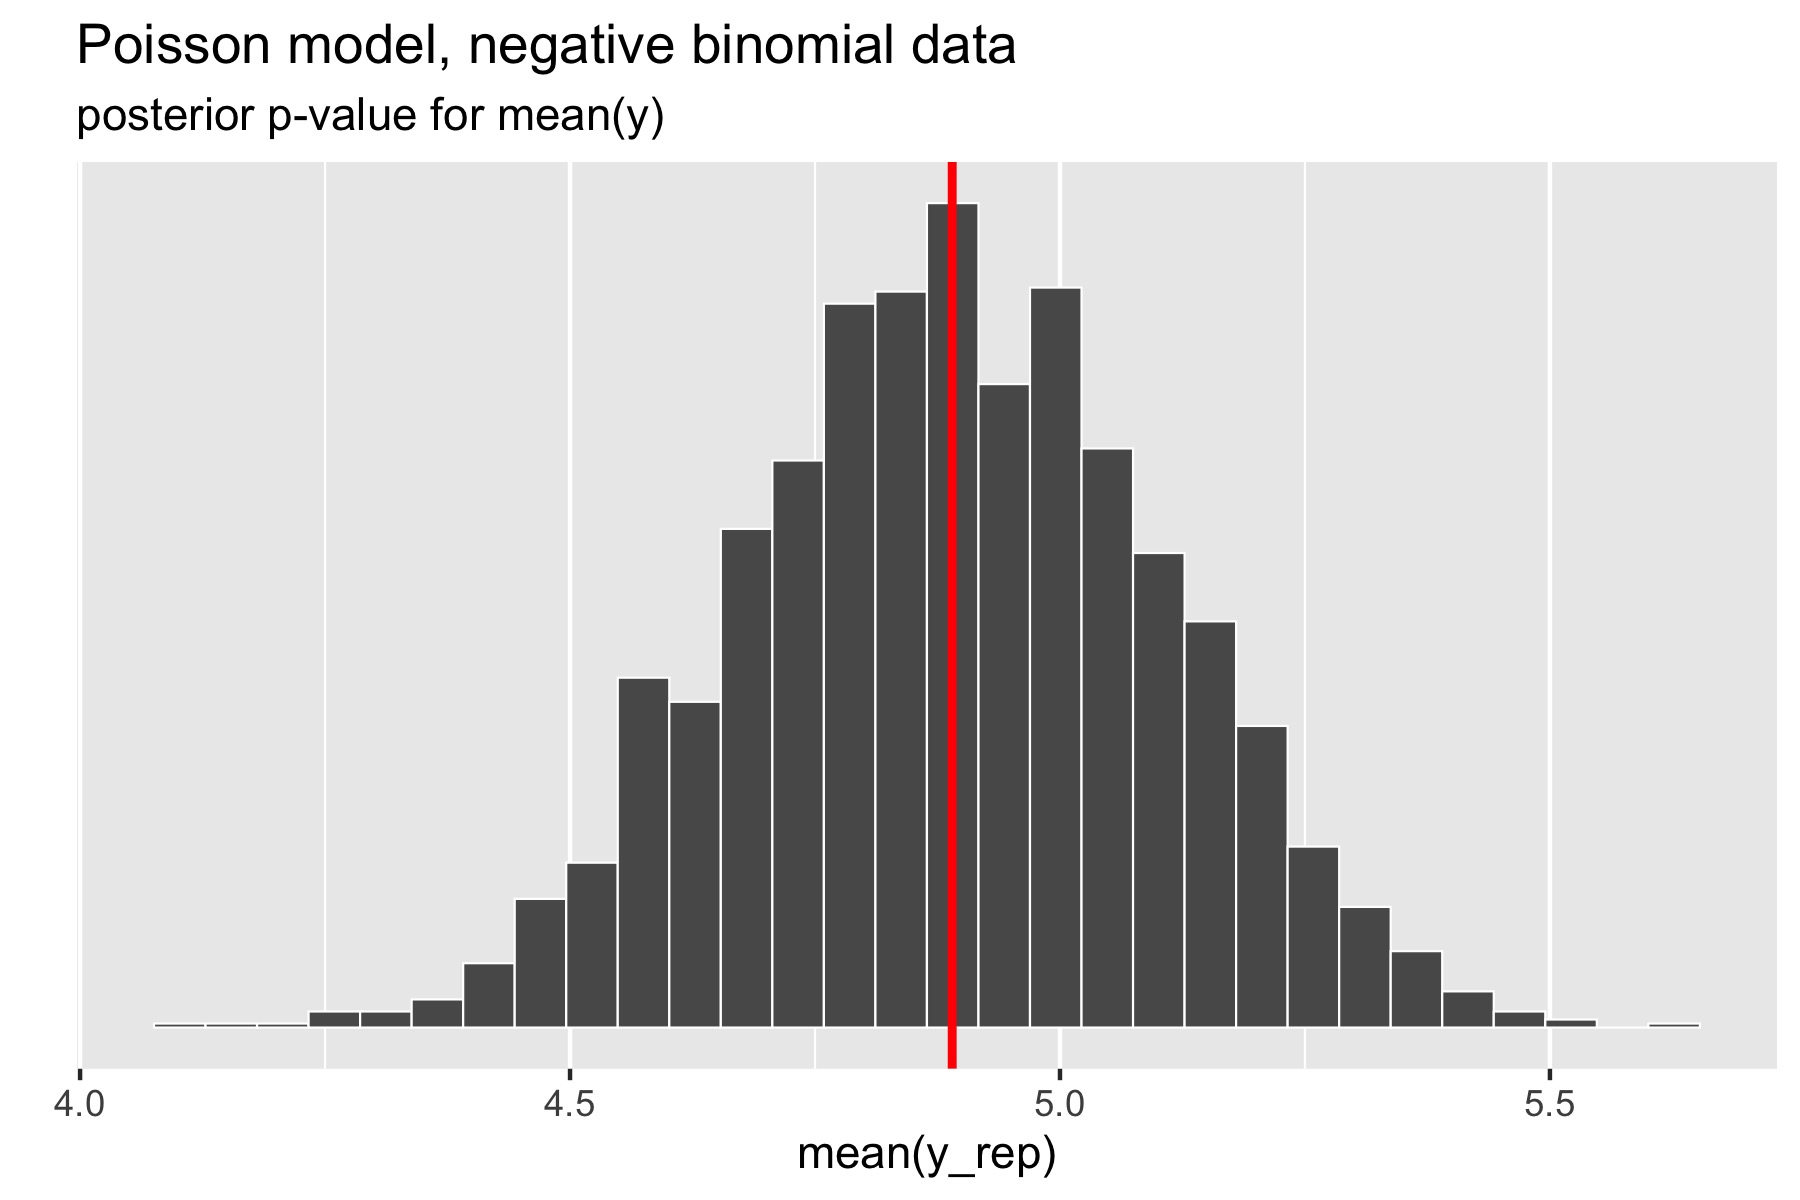
\includegraphics[width=0.5\linewidth]{./img/ppc-pvalue-nb-pois-mean} 

}

\caption{Histogram of means of replicated data sets; vertical red line at mean of original data.}\label{fig:unnamed-chunk-51}
\end{figure}

The p-value for the mean is just the percentage of replicated data
sets whose statistic is greater than or equal that of the original
data. Using a Poisson model for negative binomial data still fits the
mean well, with a posterior \(p\)-value of 0.49. In Stan terms, it is
extracted as the posterior mean of the indicator variable \texttt{mean\_gt}.

The standard deviation statistic tells a different story.

\begin{figure}

{\centering 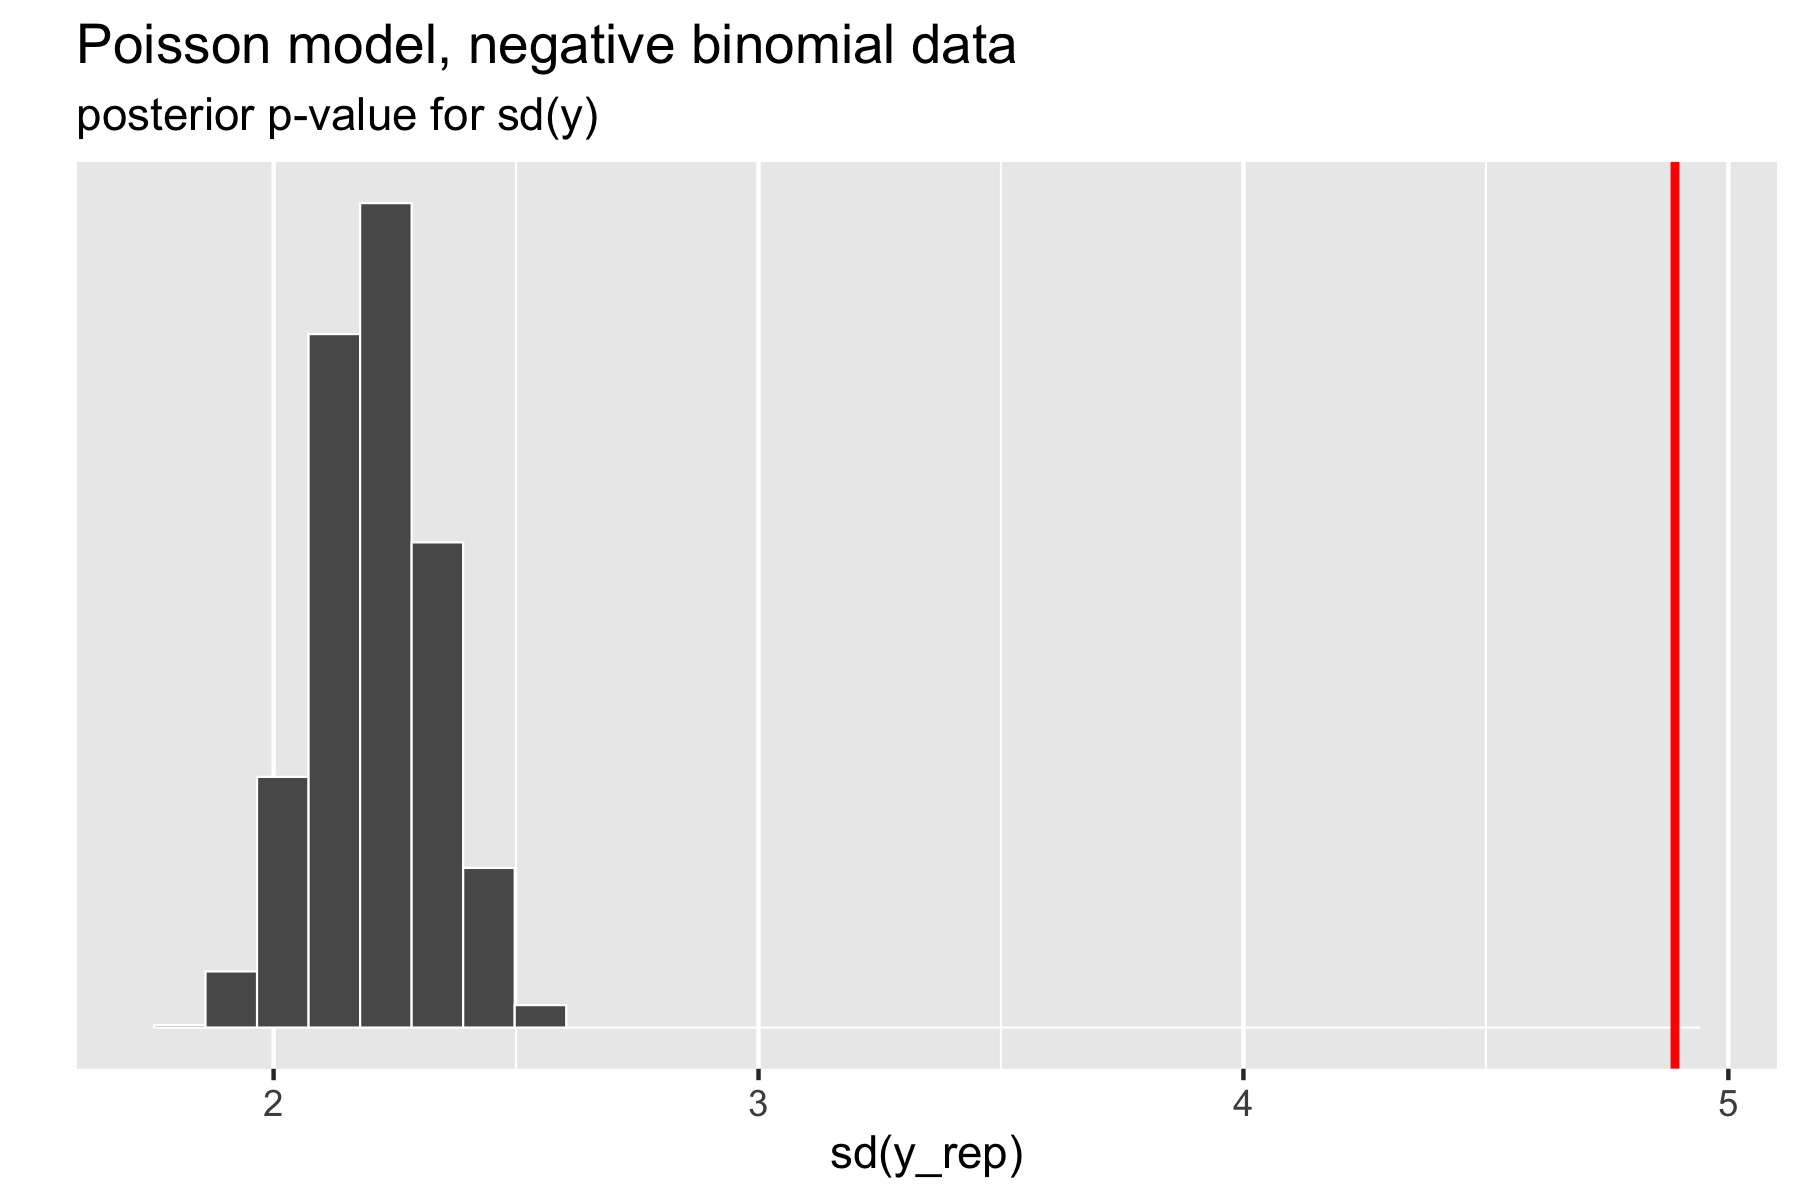
\includegraphics[width=0.5\linewidth]{./img/ppc-pvalue-nb-pois-sd} 

}

\caption{Scatterplot of standard deviations of replicated data sets; the vertical red line is at standard deviation of original data.}\label{fig:unnamed-chunk-52}
\end{figure}

Here, the original data has much higher standard deviation than any of
the replicated data sets. The resulting \(p\)-value estimated by Stan
after a large number of iterations is exactly zero (the absolute error
bounds are fine, but a lot of iterations are required to get good
relative error bounds on small \(p\)-values by sampling). In other
words, there were no posterior draws in which the replicated data set
had a standard deviation greater than or equal to that of the original
data set. Clearly, the model is not capturing the dispersion of the
original data. The point of this exercise isn't just to figure out
that there's a problem with a model, but to isolate where it is.
Seeing that the data is over-dispersed compared to the Poisson model
would be reason to fit a more general model like the negative binomial
or a latent varying effects (aka random effects) model that can
account for the over-dispersion.

\hypertarget{which-statistics-to-test}{%
\subsection{Which statistics to test?}\label{which-statistics-to-test}}

Any statistic may be used for the data, but these can be guided by the
quantities of interest in the model itself. Popular choices in
addition to mean and standard deviation are quantiles, such as the
median, 5\% or 95\% quantiles, or even the maximum or minimum value to
test extremes.

Despite the range of choices, test statistics should ideally be
ancillary, in the sense that they should be testing something other
than the fit of a parameter. For example, a simple normal model of a
data set will typically fit the mean and variance of the data quite
well as long as the prior doesn't dominate the posterior. In
contrast, a Poisson model of the same data cannot capture both the
mean and the variance of a data set if they are different, so they
bear checking in the Poisson case. As we saw with the Poisson case,
the posterior mean for the single rate parameter was located near the
data mean, not the data variance. Other distributions such as the
lognormal and gamma distribution, have means and variances that are
functions of two or more parameters.

\hypertarget{prior-predictive-checks}{%
\section{Prior predictive checks}\label{prior-predictive-checks}}

Prior predictive checks generate data according to the prior in order
to asses whether a prior is appropriate (\protect\hyperlink{ref-GabryEtAl:2019}{Gabry et al. 2019}). A
posterior predictive check generates replicated data according to the
posterior predictive distribution. In contrast, the prior predictive
check generates data according to the prior predictive distribution,
\[
y^{\textrm{sim}} \sim p(y).
\]
The prior predictive distribution is just like the posterior
predictive distribution with no observed data, so that a prior
predictive check is nothing more than the limiting case of a posterior
predictive check with no data.

This is easy to carry out mechanically by simulating parameters
\[
\theta^{\textrm{sim}} \sim p(\theta)
\]
according to the priors, then simulating data
\[
y^{\textrm{sim}} \sim p(y \mid \theta^{\textrm{sim}})
\]
according to the sampling distribution given the simulated
parameters. The result is a simulation from the joint
distribution,
\[
(y^{\textrm{sim}}, \theta^{\textrm{sim}}) \sim p(y, \theta)
\]
and thus
\[
y^{\textrm{sim}} \sim p(y)
\]
is a simulation from the prior predictive distribution.

\hypertarget{coding-prior-predictive-checks-in-stan}{%
\subsection{Coding prior predictive checks in Stan}\label{coding-prior-predictive-checks-in-stan}}

A prior predictive check is coded just like a posterior predictive
check. If a posterior predictive check has already been coded and
it's possible to set the data to be empty, then no additional coding
is necessary. The disadvantage to coding prior predictive checks as
posterior predictive checks with no data is that Markov chain Monte
Carlo will be used to sample the parameters, which is less efficient
than taking independent draws using random number generation.

Prior predictive checks can be coded entirely within the generated
quantities block using random number generation. The resulting draws
will be independent. Predictors must be read in from the actual data
set---they do not have a generative model from which to be simulated.
For a Poisson regression, prior predictive sampling can be
encoded as the following complete Stan program.

\begin{Shaded}
\begin{Highlighting}[]
\KeywordTok{data}\NormalTok{ \{}
  \DataTypeTok{int}\NormalTok{\textless{}}\KeywordTok{lower}\NormalTok{=}\DecValTok{0}\NormalTok{\textgreater{} N;}
  \DataTypeTok{vector}\NormalTok{[N] x;}
\NormalTok{\}}
\KeywordTok{generated quantities}\NormalTok{ \{}
  \DataTypeTok{real}\NormalTok{ alpha = normal\_rng(}\DecValTok{0}\NormalTok{, }\DecValTok{1}\NormalTok{);}
  \DataTypeTok{real}\NormalTok{ beta = normal\_rng(}\DecValTok{0}\NormalTok{, }\DecValTok{1}\NormalTok{);}
  \DataTypeTok{array}\NormalTok{[N] }\DataTypeTok{real}\NormalTok{ y\_sim = poisson\_log\_rng(alpha + beta * x);}
\NormalTok{\}}
\end{Highlighting}
\end{Shaded}

Running this program using Stan's fixed-parameter sampler
yields draws from the prior. These may be plotted to
consider their appropriateness.

\hypertarget{example-of-prior-predictive-checks}{%
\section{Example of prior predictive checks}\label{example-of-prior-predictive-checks}}

Suppose we have a model for a football (aka soccer) league where there
are \(J\) teams. Each team has a scoring rate \(\lambda_j\) and in each
game will be assumed to score \(\textrm{poisson}(\lambda_j)\) points.
Yes, this model completely ignores defense. Suppose the modeler does
not want to ``put their thumb on the scale'' and would rather ``let the
data speak for themselves'' and so uses a prior with very wide tails,
because it seems uninformative, such as the widely deployed
\[
\lambda_j \sim \textrm{gamma}(\epsilon_1, \epsilon_2).
\]
This is not just a manufactured example; \emph{The BUGS Book}
recommends setting \(\epsilon = (0.5, 0.00001)\), which
corresponds to a Jeffreys prior for a Poisson rate parameter prior
(\protect\hyperlink{ref-LunnEtAl:2012}{Lunn et al. 2012, 85}).

Suppose the league plays a round-robin tournament wherein every team
plays every other team. The following Stan model generates random team
abilities and the results of such a round-robin tournament, which may
be used to perform prior predictive checks.

\begin{Shaded}
\begin{Highlighting}[]
\KeywordTok{data}\NormalTok{ \{}
  \DataTypeTok{int}\NormalTok{\textless{}}\KeywordTok{lower}\NormalTok{=}\DecValTok{0}\NormalTok{\textgreater{} J;}
  \DataTypeTok{array}\NormalTok{[}\DecValTok{2}\NormalTok{] }\DataTypeTok{real}\NormalTok{\textless{}}\KeywordTok{lower}\NormalTok{=}\DecValTok{0}\NormalTok{\textgreater{} epsilon;}
\NormalTok{\}}
\KeywordTok{generated quantities}\NormalTok{ \{}
  \DataTypeTok{array}\NormalTok{[J] }\DataTypeTok{real}\NormalTok{\textless{}}\KeywordTok{lower}\NormalTok{=}\DecValTok{0}\NormalTok{\textgreater{} lambda;}
  \DataTypeTok{array}\NormalTok{[J, J] }\DataTypeTok{int}\NormalTok{ y;}
  \ControlFlowTok{for}\NormalTok{ (j }\ControlFlowTok{in} \DecValTok{1}\NormalTok{:J) lambda[j] = gamma\_rng(epsilon[}\DecValTok{1}\NormalTok{], epsilon[}\DecValTok{2}\NormalTok{]);}
  \ControlFlowTok{for}\NormalTok{ (i }\ControlFlowTok{in} \DecValTok{1}\NormalTok{:J) \{}
    \ControlFlowTok{for}\NormalTok{ (j }\ControlFlowTok{in} \DecValTok{1}\NormalTok{:J) \{}
\NormalTok{      y[i, j] = poisson\_rng(lambda[i]) {-} poisson\_rng(lambda[j]);}
\NormalTok{    \}}
\NormalTok{  \}}
\NormalTok{\}}
\end{Highlighting}
\end{Shaded}

In this simulation, teams play each other twice and play themselves
once. This could be made more realistic by controlling the
combinatorics to only generate a single result for each pair of teams,
of which there are \(\binom{J}{2} = \frac{J \cdot (J - 1)}{2}.\)

Using the \(\textrm{gamma}(0.5, 0.00001)\) reference prior on team
abilities, the following are the first 20 simulated point differences
for the match between the first two teams, \(y^{(1:20)}_{1, 2}\).

\begin{verbatim}
2597 -26000   5725  22496   1270   1072   4502  -2809   -302   4987
7513   7527  -3268 -12374   3828   -158 -29889   2986  -1392     66
\end{verbatim}

That's some pretty highly scoring football games being simulated; all
but one has a score differential greater than 100! In other words, this
\(\textrm{gamma}(0.5, 0.00001)\) prior is putting around 95\% of its
weight on score differentials above 100. Given that two teams
combined rarely score 10 points, this prior is way out of line with
prior knowledge about football matches; it is not only consistent with
outcomes that have never occurred in the history of the sport, it puts
most of the prior probability mass there.

The posterior predictive distribution can be strongly affected by the
prior when there is not much observed data and substantial prior mass
is concentrated around infeasible values (\protect\hyperlink{ref-Gelman:2006}{A. Gelman 2006}).

Just as with posterior predictive distributions, any statistics of the
generated data may be evaluated. Here, the focus was on score
difference between a single pair of teams, but it could've been on
maximums, minimums, averages, variances, etc.

In this textbook example, the prior is univariate and directly related
to the expected number of points scored, and could thus be directly
inspected for consistency with prior knowledge about scoring rates in
football. There will not be the same kind of direct connection when
the prior and sampling distributions are multivariate. In these more
challenging situations, prior predictive checks are an easy way to get
a handle on the implications of a prior in terms of what it says the
data is going to look like; for a more complex application involving
spatially heterogeneous air pollution concentration, see (\protect\hyperlink{ref-GabryEtAl:2019}{Gabry et al. 2019}).

Prior predictive checks can also be compared with the data, but one
should not expect them to be calibrated in the same way as posterior
predictive checks. That would require guessing the posterior and
encoding it in the prior. The goal is make sure the prior is not so
wide that it will pull probability mass away from feasible values.

\hypertarget{mixed-replication}{%
\section{Mixed predictive replication for hierarchical models}\label{mixed-replication}}

Andrew Gelman, Meng, and Stern (\protect\hyperlink{ref-GelmanEtAl:1996}{1996}) discuss the case of mixed replication for
hierarchical models in which the hyperparameters remain fixed, but
varying effects are replicated. This is neither a purely prior nor
purely posterior predictive check, but falls somewhere in between.

For example, consider a simple varying intercept logistic regression,
with intercepts \(\alpha_k\) for \(k \in 1:K\). Each data item
\(y_n \in \{ 0, 1 \}\) is assumed to correspond to group \(kk_n \in 1:K.\)
The sampling distribution is thus
\[
y_n \sim \textrm{bernoulli}(\textrm{logit}^{-1}(\alpha_{kk[n]})).
\]
The varying intercepts have a hierarchical normal prior,
\[
\alpha_k \sim \textrm{normal}(\mu, \sigma).
\]
The hyperparameters are themselves given weakly informative priors,
\begin{eqnarray*}
\mu & \sim & \textrm{normal}(0, 2)
\\[4pt]
\sigma & \sim & \textrm{lognormal}(0, 1).
\end{eqnarray*}

Like in a posterior predictive check, the hyperparameters \(\mu\) and
\(\sigma\) are drawn from the posterior,
\[
\mu^{(m)}, \sigma^{(m)} \sim p(\mu, \sigma \mid y)
\]
Like in a prior predictive check, replicated values of \(\alpha\) are
drawn from the hyperparameters,
\[
\alpha^{\textrm{rep}(m)}_k \sim \textrm{normal}(\alpha_k \mid
\mu^{(m)}, \sigma^{(m)}).
\]
The data items are then each replicated using the replicated intercepts,
\[
y^{\textrm{rep}(m)}_n \sim
\textrm{bernoulli}
  (\textrm{logit}^{-1}(\alpha^{\textrm{rep}(m)}_{kk[n]})).
\]
Thus the \(y^{\textrm{rep}(m)}\) can be seen as a kind of posterior
predictive replication of observations from new groups that were not
among the original \(K\) groups.

In Stan, mixed predictive replications \(y^{\textrm{rep}(m)}\) can be
programmed directly.

\begin{Shaded}
\begin{Highlighting}[]
\KeywordTok{data}\NormalTok{ \{}
  \DataTypeTok{int}\NormalTok{\textless{}}\KeywordTok{lower}\NormalTok{=}\DecValTok{0}\NormalTok{\textgreater{} K;}
  \DataTypeTok{int}\NormalTok{\textless{}}\KeywordTok{lower}\NormalTok{=}\DecValTok{0}\NormalTok{\textgreater{} N;}
  \DataTypeTok{array}\NormalTok{[N] }\DataTypeTok{int}\NormalTok{\textless{}}\KeywordTok{lower}\NormalTok{=}\DecValTok{1}\NormalTok{, }\KeywordTok{upper}\NormalTok{=K\textgreater{} kk;}
  \DataTypeTok{array}\NormalTok{[N] }\DataTypeTok{int}\NormalTok{\textless{}}\KeywordTok{lower}\NormalTok{=}\DecValTok{0}\NormalTok{, }\KeywordTok{upper}\NormalTok{=}\DecValTok{1}\NormalTok{\textgreater{} y;}
\NormalTok{\}}
\KeywordTok{parameters}\NormalTok{ \{}
  \DataTypeTok{real}\NormalTok{ mu;}
  \DataTypeTok{real}\NormalTok{\textless{}}\KeywordTok{lower}\NormalTok{=}\DecValTok{0}\NormalTok{\textgreater{} sigma;}
  \DataTypeTok{vector}\NormalTok{\textless{}}\DataTypeTok{offset}\NormalTok{=mu, }\DataTypeTok{multiplier}\NormalTok{=sigma\textgreater{}[K] alpha;}
\NormalTok{\}}
\KeywordTok{model}\NormalTok{ \{}
\NormalTok{  mu \textasciitilde{} normal(}\DecValTok{0}\NormalTok{, }\DecValTok{2}\NormalTok{);               }\CommentTok{// hyperprior}
\NormalTok{  sigma \textasciitilde{} lognormal(}\DecValTok{0}\NormalTok{, }\DecValTok{1}\NormalTok{);}
\NormalTok{  alpha \textasciitilde{} normal(mu, sigma);       }\CommentTok{// hierarchical prior}
\NormalTok{  y \textasciitilde{} bernoulli\_logit(alpha[kk]);  }\CommentTok{// sampling distribution}
\NormalTok{\}}
\KeywordTok{generated quantities}\NormalTok{ \{}
  \CommentTok{// alpha replicated;  mu and sigma not replicated}
  \DataTypeTok{array}\NormalTok{[K] }\DataTypeTok{real}\NormalTok{ alpha\_rep}
\NormalTok{    = normal\_rng(rep\_vector(mu, K), sigma);}
  \DataTypeTok{array}\NormalTok{[N] }\DataTypeTok{int}\NormalTok{\textless{}}\KeywordTok{lower}\NormalTok{=}\DecValTok{0}\NormalTok{, }\KeywordTok{upper}\NormalTok{=}\DecValTok{1}\NormalTok{\textgreater{} y\_rep}
\NormalTok{    = bernoulli\_logit\_rng(alpha\_rep[kk]);}
\NormalTok{\}}
\end{Highlighting}
\end{Shaded}

\hypertarget{joint-model-representation}{%
\section{Joint model representation}\label{joint-model-representation}}

Following Andrew Gelman, Meng, and Stern (\protect\hyperlink{ref-GelmanEtAl:1996}{1996}), prior, posterior, and mixed replications
may all be defined as posteriors from joint models over parameters and
observed and replicated data.

\hypertarget{posterior-predictive-model}{%
\subsection{Posterior predictive model}\label{posterior-predictive-model}}

For example, posterior predictive replication may be formulated
using sampling notation as follows.
\begin{eqnarray*}
\theta & \sim & p(\theta)
\\[2pt]
y & \sim & p(y \mid \theta)
\\[2pt]
y^{\textrm{rep}} & \sim & p(y \mid \theta)
\end{eqnarray*}
The heavily overloaded sampling notation is meant to indicate that
both \(y\) and \(y^{\textrm{rep}}\) are drawn from the same distribution,
or more formally using capital letters to distinguish random
variables, that the conditional densities \(p_{Y^{\textrm{rep}} \mid \Theta}\) and \(p_{Y \mid \Theta}\) are the same.

The joint density is
\[
p(\theta, y, y^{\textrm{rep}})
= p(\theta) \cdot p(y \mid \theta) \cdot p(y^{\textrm{rep}} \mid \theta).
\]
This again is assuming that the two distributions for \(y\) and
\(y^{\textrm{rep}}\) are identical.

The variable \(y\) is observed, with the predictive simulation
\(y^{\textrm{rep}}\) and parameter vector \(\theta\) not observed. The
posterior is \(p(y^{\textrm{rep}}, \theta \mid y)\). Given draws from
the posterior, the posterior predictive simulations \(y^{\textrm{rep}}\)
are retained.

\hypertarget{prior-predictive-model}{%
\subsection{Prior predictive model}\label{prior-predictive-model}}

The prior predictive model simply drops the data component of the
posterior predictive model.\\
\begin{eqnarray*}
\theta & \sim & p(\theta)
\\[2pt]
y^{\textrm{rep}} & \sim & p(y \mid \theta)
\end{eqnarray*}
This corresponds to the joint density
\[
p(\theta, y^{\textrm{rep}}) = p(\theta) \cdot p(y^{\textrm{rep}} \mid
\theta).
\]

It is typically straightforward to draw \(\theta\) from the prior and
\(y^{\textrm{rep}}\) from the sampling distribution given \(\theta\)
efficiently. In cases where it is not, the model may be coded and
executed just as the posterior predictive model, only with no data.

\hypertarget{mixed-replication-for-hierarchical-models}{%
\subsection{Mixed replication for hierarchical models}\label{mixed-replication-for-hierarchical-models}}

The mixed replication corresponds to the model
\begin{eqnarray*}
\phi & \sim & p(\phi)
\\[2pt]
\alpha & \sim & p(\alpha \mid \phi)
\\[2pt]
y & \sim & p(y \mid \alpha)
\\[2pt]
\alpha^{\textrm{rep}} & \sim & p(\alpha \mid \phi)
\\[2pt]
y^{\textrm{rep}} & \sim & p(y \mid \phi)
\end{eqnarray*}
The notation here is meant to indicate that \(\alpha\) and
\(\alpha^{\textrm{rep}}\) have identical distributions, as do \(y\) and
\(y^{\textrm{rep}}\).

This corresponds to a joint model
\[
p(\phi, \alpha, \alpha^{\textrm{rep}}, y, y^{\textrm{rep}})
=
p(\phi)
\cdot p(\alpha \mid \phi)
\cdot p(y \mid \alpha)
\cdot p(\alpha^{\textrm{rep}} \mid \phi)
\cdot p(y^{\textrm{rep}} \mid \alpha^{\textrm{rep}}),
\]
where \(y\) is the only observed variable, \(\alpha\) contains the
lower-level parameters and \(\phi\) the hyperparameters. Note that
\(\phi\) is not replicated and instead appears in the distribution for
both \(\alpha\) and \(\alpha^{\textrm{rep}}\).

The posterior is \(p(\phi, \alpha, \alpha^{\textrm{rep}}, y^{\textrm{rep}} \mid y)\). From posterior draws, the posterior
predictive simulations \(y^{\textrm{rep}}\) are kept.

\hypertarget{held-out-evaluation-and-cross-validation}{%
\chapter{Held-Out Evaluation and Cross-Validation}\label{held-out-evaluation-and-cross-validation}}

Held-out evaluation involves splitting a data set into two parts, a
training data set and a test data set. The training data is used to
estimate the model and the test data is used for evaluation. Held-out
evaluation is commonly used to declare winners in predictive modeling
competitions such as those run by \href{https://kaggle.com}{Kaggle}.

Cross-validation involves repeated held-out evaluations performed by
partitioning a single data set in different ways. The training/test
split can be done either by randomly selecting the test set, or by
partitioning the data set into several equally-sized subsets and then
using each subset in turn as the test data with the other folds as
training data.

Held-out evaluation and cross-validation may involve any kind
of predictive statistics, with common choices being the predictive log
density on test data, squared error of parameter estimates, or accuracy
in a classification task.

\hypertarget{evaluating-posterior-predictive.section}{%
\section{Evaluating posterior predictive densities}\label{evaluating-posterior-predictive.section}}

Given training data \((x, y)\) consisting of parallel sequences of
predictors and observations and test data \((\tilde{x}, \tilde{y})\) of
the same structure, the posterior predictive density is
\[
p(\tilde{y} \mid \tilde{x}, x, y)
=
\int
  p(\tilde{y} \mid \tilde{x}, \theta)
  \cdot p(\theta \mid x, y)
\, \textrm{d}\theta,
\]

where \(\theta\) is the vector of model parameters. This predictive
density is the density of the test observations, conditioned on both
the test predictors \(\tilde{x}\) and the training data \((x, y).\)

This integral may be calculated with Monte Carlo methods as usual,
\[
p(\tilde{y} \mid \tilde{x}, x, y)
\approx
\frac{1}{M} \sum_{m = 1}^M p(\tilde{y} \mid \tilde{x}, \theta^{(m)}),
\]
where the \(\theta^{(m)} \sim p(\theta \mid x, y)\) are draws from the
posterior given only the training data \((x, y).\)

To avoid underflow in calculations, it will be more stable
to compute densities on the log scale. Taking the logarithm and
pushing it through results in a stable computation,
\begin{eqnarray*}
\log p(\tilde{y} \mid \tilde{x}, x, y)
& \approx &
\log \frac{1}{M} \sum_{m = 1}^M p(\tilde{y} \mid \tilde{x}, \theta^{(m)}),
\\[4pt]
& = & -\log M + \log \sum_{m = 1}^M p(\tilde{y} \mid \tilde{x}, \theta^{(m)}),
\\[4pt]
& = & -\log M + \log \sum_{m = 1}^M \exp(\log p(\tilde{y} \mid \tilde{x}, \theta^{(m)}))
\\[4pt]
& = & -\log M + \textrm{log-sum-exp}_{m = 1}^M \log p(\tilde{y} \mid \tilde{x}, \theta^{(m)})
\end{eqnarray*}
where the log sum of exponentials function is defined so as
to make the above equation hold,
\[
\textrm{log-sum-exp}_{m = 1}^M \, \mu_m
= \log \sum_{m=1}^M \exp(\mu_m).
\]
The log sum of exponentials function can be implemented so as to avoid
underflow and maintain high arithmetic precision as
\[
\textrm{log-sum-exp}_{m = 1}^M \mu_m
= \textrm{max}(\mu)
+ \log \sum_{m = 1}^M \exp(\mu_m - \textrm{max}(\mu)).
\]
Pulling the maximum out preserves all of its precision. By
subtracting the maximum, the terms \(\mu_m - \textrm{max}(\mu) \leq 0\),
and thus will not overflow.

\hypertarget{stan-program-1}{%
\subsection{Stan program}\label{stan-program-1}}

To evaluate the log predictive density of a model, it suffices to
implement the log predictive density of the test data in the generated quantities
block. The log sum of exponentials calculation must be done on the
outside of Stan using the posterior draws of \(\log p(\tilde{y} \mid \tilde{x}, \theta^{(m)}).\)

Here is the code for evaluating the log posterior predictive density
in a simple linear regression of the test data \(\tilde{y}\) given
predictors \(\tilde{x}\) and training data \((x, y).\)

\begin{Shaded}
\begin{Highlighting}[]
\KeywordTok{data}\NormalTok{ \{}
  \DataTypeTok{int}\NormalTok{\textless{}}\KeywordTok{lower}\NormalTok{=}\DecValTok{0}\NormalTok{\textgreater{} N;}
  \DataTypeTok{vector}\NormalTok{[N] y;}
  \DataTypeTok{vector}\NormalTok{[N] x;}
  \DataTypeTok{int}\NormalTok{\textless{}}\KeywordTok{lower}\NormalTok{=}\DecValTok{0}\NormalTok{\textgreater{} N\_tilde;}
  \DataTypeTok{vector}\NormalTok{[N\_tilde] x\_tilde;}
  \DataTypeTok{vector}\NormalTok{[N\_tilde] y\_tilde;}
\NormalTok{\}}
\KeywordTok{parameters}\NormalTok{ \{}
  \DataTypeTok{real}\NormalTok{ alpha;}
  \DataTypeTok{real}\NormalTok{ beta;}
  \DataTypeTok{real}\NormalTok{\textless{}}\KeywordTok{lower}\NormalTok{=}\DecValTok{0}\NormalTok{\textgreater{} sigma;}
\NormalTok{\}}
\KeywordTok{model}\NormalTok{ \{}
\NormalTok{  y \textasciitilde{} normal(alpha + beta * x, sigma);}
\NormalTok{\}}
\KeywordTok{generated quantities}\NormalTok{ \{}
  \DataTypeTok{real}\NormalTok{ log\_p = normal\_lpdf(y\_tilde | alpha + beta * x\_tilde, sigma);}
\NormalTok{\}}
\end{Highlighting}
\end{Shaded}

Only the training data \texttt{x} and \texttt{y} are used in the model block. The
test data \texttt{y\_tilde} and test predictors \texttt{x\_tilde} appear in only the
generated quantities block. Thus the program is not cheating by using
the test data during training. Although this model does not do so,
it would be fair to use \texttt{x\_tilde} in the model block---only the
test observations \texttt{y\_tilde} are unknown before they are predicted.

Given \(M\) posterior draws from Stan, the sequence \texttt{log\_p{[}1:M{]}} will be
available, so that the log posterior predictive density of the test
data given training data and predictors is just \texttt{log\_sum\_exp(log\_p)\ -\ log(M)}.

\hypertarget{estimation-error}{%
\section{Estimation error}\label{estimation-error}}

\hypertarget{parameter-estimates}{%
\subsection{Parameter estimates}\label{parameter-estimates}}

Estimation is usually considered for unknown parameters. If the data
from which the parameters were estimated came from simulated data, the
true value of the parameters may be known. If \(\theta\) is the true
value and \(\hat{\theta}\) the estimate, then error is just the
difference between the prediction and the true value,
\[
\textrm{err} = \hat{\theta} - \theta.
\]

If the estimate is larger than the true value, the error is positive,
and if it's smaller, then error is negative. If an estimator's
unbiased, then expected error is zero. So typically, absolute error
or squared error are used, which will always have positive
expectations for an imperfect estimator. \emph{Absolute error} is defined as
\[
\textrm{abs-err} = \left| \hat{\theta} - \theta \right|
\]
and \emph{squared error} as
\[
\textrm{sq-err} = \left( \hat{\theta} - \theta \right)^2.
\]
Gneiting and Raftery (\protect\hyperlink{ref-GneitingRaftery:2007}{2007}) provide a thorough overview of such scoring rules
and their properties.

Bayesian posterior means minimize expected square error, whereas
posterior medians minimize expected absolute error. Estimates based
on modes rather than probability, such as (penalized) maximum
likelihood estimates or maximum a posterior estimates, do not have
these properties.

\hypertarget{predictive-estimates}{%
\subsection{Predictive estimates}\label{predictive-estimates}}

In addition to parameters, other unknown quantities may be estimated,
such as the score of a football match or the effect of a medical
treatment given to a subject. In these cases, square error is defined
in the same way. If there are multiple exchangeable outcomes being
estimated, \(z_1, \ldots, z_N,\) then it is common to report \emph{mean square
error} (MSE),
\[
\textrm{mse}
= \frac{1}{N} \sum_{n = 1}^N \left( \hat{z}_n - z_n\right)^2.
\]
To put the error back on the scale of the original value, the square
root may be applied, resulting in what is known prosaically
as \emph{root mean square error} (RMSE),
\[
\textrm{rmse} = \sqrt{\textrm{mean-sq-err}}.
\]

\hypertarget{predictive-estimates-in-stan}{%
\subsection{Predictive estimates in Stan}\label{predictive-estimates-in-stan}}

Consider a simple linear regression model, parameters for the
intercept \(\alpha\) and slope \(\beta\), along with predictors
\(\tilde{x}_n\). The standard Bayesian estimate is the expected value
of \(\tilde{y}\) given the predictors and training data,
\begin{eqnarray*}
\hat{\tilde{y}}_n
& = & \mathbb{E}[\tilde{y}_n \mid \tilde{x}_n, x, y]
\\[4pt]
& \approx & \frac{1}{M} \sum_{m = 1}^M \tilde{y}_n^{(m)}
\end{eqnarray*}
where \(\tilde{y}_n^{(m)}\) is drawn from the sampling distribution
\[
\tilde{y}_n^{(m)}
\sim p(\tilde{y}_n \mid \tilde{x}_n, \alpha^{(m)}, \beta^{(m)}),
\]
for parameters \(\alpha^{(m)}\) and \(\beta^{(m)}\) drawn from the posterior,
\[
(\alpha^{(m)}, \beta^{(m)}) \sim p(\alpha, \beta \mid x, y).
\]

In the linear regression case, two stages of simplification can be
carried out, the first of which helpfully reduces the variance of the
estimator. First, rather than averaging samples \(\tilde{y}_n^{(m)}\),
the same result is obtained by averaging linear predictions,
\begin{eqnarray*}
\hat{\tilde{y}}_n
& = & \mathbb{E}\left[
          \alpha + \beta \cdot \tilde{x}_n
          \mid \tilde{x}_n, x, y
       \right]
\\[4pt]
& \approx &
\frac{1}{M} \sum_{m = 1}^M
  \alpha^{(m)} + \beta^{(m)} \cdot \tilde{x}_n
\end{eqnarray*}
This is possible because
\[
\tilde{y}_n^{(m)} \sim \textrm{normal}(\tilde{y}_n \mid \alpha^{(m)} +
\beta^{(m)} \cdot \tilde{x}_n, \sigma^{(m)}),
\]
and the normal distribution has symmetric error so that the expectation of
\(\tilde{y}_n^{(m)}\) is the same as \(\alpha^{(m)} + \beta^{(m)} \cdot \tilde{x}_n\). Replacing the sampled quantity \(\tilde{y}_n^{(m)}\) with
its expectation is a general variance reduction technique for Monte
Carlo estimates known as \emph{Rao-Blackwellization} (\protect\hyperlink{ref-Rao:1945}{Rao 1945}; \protect\hyperlink{ref-Blackwell:1947}{Blackwell 1947}).

In the linear case, because the predictor is linear in the
coefficients, the estimate can be further simplified to use the
estimated coefficients,
\begin{eqnarray*}
\tilde{y}_n^{(m)}
& \approx &
\frac{1}{M} \sum_{m = 1}^M
  \left( \alpha^{(m)} + \beta^{(m)} \cdot \tilde{x}_n \right)
\\[4pt]
& = & \frac{1}{M} \sum_{m = 1}^M \alpha^{(m)}
      + \frac{1}{M} \sum_{m = 1}^M (\beta^{(m)} \cdot \tilde{x}_n)
\\[4pt]
& = & \frac{1}{M} \sum_{m = 1}^M \alpha^{(m)}
      + \left( \frac{1}{M} \sum_{m = 1}^M \beta^{(m)}\right) \cdot \tilde{x}_n
\\[4pt]
& = & \hat{\alpha} + \hat{\beta} \cdot \tilde{x}_n.
\end{eqnarray*}

In Stan, only the first of the two steps (the important variance
reduction step) can be coded in the object model. The linear
predictor is defined in the generated quantities block.

\begin{Shaded}
\begin{Highlighting}[]
\KeywordTok{data}\NormalTok{ \{}
  \DataTypeTok{int}\NormalTok{\textless{}}\KeywordTok{lower}\NormalTok{=}\DecValTok{0}\NormalTok{\textgreater{} N\_tilde;}
  \DataTypeTok{vector}\NormalTok{[N\_tilde] x\_tilde;}
  \CommentTok{// ...}
\NormalTok{\}}
\CommentTok{// ...}
\KeywordTok{generated quantities}\NormalTok{ \{}
  \DataTypeTok{vector}\NormalTok{[N\_tilde] tilde\_y = alpha + beta * x\_tilde;}
\NormalTok{\}}
\end{Highlighting}
\end{Shaded}

The posterior mean of \texttt{tilde\_y} calculated by Stan is the Bayesian
estimate \(\hat{\tilde{y}}.\) The posterior median may also be
calculated and used as an estimate, though square error and the
posterior mean are more commonly reported.

\hypertarget{cross-validation}{%
\section{Cross-validation}\label{cross-validation}}

Cross-validation involves choosing multiple subsets of a data set as
the test set and using the other data as training. This can be done
by partitioning the data and using each subset in turn as the test set
with the remaining subsets as training data. A partition into ten
subsets is common to reduce computational overhead. In the limit,
when the test set is just a single item, the result is known as
leave-one-out (LOO) cross-validation (\protect\hyperlink{ref-VehtariEtAl:2017}{Vehtari, Gelman, and Gabry 2017}).

Partitioning the data and reusing the partitions is very fiddly in the
indexes and may not lead to even divisions of the data. It's far
easier to use random partitions, which support arbitrarily sized
test/training splits and can be easily implemented in Stan. The
drawback is that the variance of the resulting estimate is higher than
with a balanced block partition.

\hypertarget{stan-implementation-with-random-folds}{%
\subsection{Stan implementation with random folds}\label{stan-implementation-with-random-folds}}

For the simple linear regression model, randomized cross-validation
can be implemented in a single model. To randomly permute a vector in
Stan, the simplest approach is the following.

\begin{Shaded}
\begin{Highlighting}[]
\KeywordTok{functions}\NormalTok{ \{}
  \DataTypeTok{array}\NormalTok{[] }\DataTypeTok{int}\NormalTok{ permutation\_rng(}\DataTypeTok{int}\NormalTok{ N) \{}
     \DataTypeTok{int}\NormalTok{ N = rows(x);}
     \DataTypeTok{array}\NormalTok{[N] }\DataTypeTok{int}\NormalTok{ y;}
     \ControlFlowTok{for}\NormalTok{ (n }\ControlFlowTok{in} \DecValTok{1}\NormalTok{:N) \{}
\NormalTok{       y[n] = n;}
\NormalTok{     \}}
     \DataTypeTok{vector}\NormalTok{[N] theta = rep\_vector(}\FloatTok{1.0}\NormalTok{ / N, N);}
     \ControlFlowTok{for}\NormalTok{ (n }\ControlFlowTok{in} \DecValTok{1}\NormalTok{:rows(y)) \{}
       \DataTypeTok{int}\NormalTok{ i = categorical\_rng(theta);}
\NormalTok{     \}}
      \DataTypeTok{array}\NormalTok{[n] }\DataTypeTok{int}\NormalTok{ temp = y;}
\NormalTok{      y[n] = y[i];}
\NormalTok{      y[i] = temp;}
\NormalTok{     \}}
     \ControlFlowTok{return}\NormalTok{ y;}
\NormalTok{  \}}
\NormalTok{\}}
\end{Highlighting}
\end{Shaded}

The name of the function must end in \texttt{\_rng} because it uses other
random functions internally. This will restrict its usage to the
transformed data and generated quantities block. The code walks
through the vector exchanging each item with another randomly chosen
item, resulting in a uniformly drawn permutation of the integers
\texttt{1:N}.\footnote{The traditional approach is to walk through a vector and replace each item with a random element from the remaining elements, which is guaranteed to only move each item once. This was not done here as it'd require new categorical \texttt{theta} because Stan does not have a uniform discrete RNG built in.}

The transformed data block uses the permutation RNG to generate
training data and test data by taking prefixes and suffixes of the
permuted data.

\begin{Shaded}
\begin{Highlighting}[]
\KeywordTok{data}\NormalTok{ \{}
  \DataTypeTok{int}\NormalTok{\textless{}}\KeywordTok{lower}\NormalTok{=}\DecValTok{0}\NormalTok{\textgreater{} N;}
  \DataTypeTok{vector}\NormalTok{[N] x;}
  \DataTypeTok{vector}\NormalTok{[N] y;}
  \DataTypeTok{int}\NormalTok{\textless{}}\KeywordTok{lower}\NormalTok{=}\DecValTok{0}\NormalTok{, }\KeywordTok{upper}\NormalTok{=N\textgreater{} N\_test;}
\NormalTok{\}}
\KeywordTok{transformed data}\NormalTok{ \{}
  \DataTypeTok{int}\NormalTok{ N\_train = N {-} N\_test;}
  \DataTypeTok{array}\NormalTok{[N] }\DataTypeTok{int}\NormalTok{ permutation = permutation\_rng(N);}
  \DataTypeTok{vector}\NormalTok{[N\_train] x\_train = x[permutation[}\DecValTok{1}\NormalTok{ : N\_train]];}
  \DataTypeTok{vector}\NormalTok{[N\_train] y\_train = y[permutation[}\DecValTok{1}\NormalTok{ : N\_train]];}
  \DataTypeTok{vector}\NormalTok{[N\_test] x\_test = x[permutation[N\_train + }\DecValTok{1}\NormalTok{ : N]];}
  \DataTypeTok{vector}\NormalTok{[N\_test] y\_test = y[permutation[N\_train + }\DecValTok{1}\NormalTok{ : N]];}
\NormalTok{\}}
\end{Highlighting}
\end{Shaded}

Recall that in Stan, \texttt{permutation{[}1:N\_train{]}} is an array of integers,
so that \texttt{x{[}permutation{[}1\ :\ N\_train{]}{]}} is a vector defined for \texttt{i\ in\ 1:N\_train}
by

\begin{Shaded}
\begin{Highlighting}[]
\NormalTok{x[permutation[}\DecValTok{1}\NormalTok{ : N\_train]][i] = x[permutation[}\DecValTok{1}\NormalTok{:N\_train][i]]}
\NormalTok{                               = x[permutation[i]]}
\end{Highlighting}
\end{Shaded}

Given the test/train split, the rest of the model is straightforward.

\begin{Shaded}
\begin{Highlighting}[]
\KeywordTok{parameters}\NormalTok{ \{}
  \DataTypeTok{real}\NormalTok{ alpha;}
  \DataTypeTok{real}\NormalTok{ beta;}
  \DataTypeTok{real}\NormalTok{\textless{}}\KeywordTok{lower}\NormalTok{=}\DecValTok{0}\NormalTok{\textgreater{} sigma;}
\NormalTok{\}}
\KeywordTok{model}\NormalTok{ \{}
\NormalTok{  y\_train \textasciitilde{} normal(alpha + beta * x\_train, sigma);}
\NormalTok{  \{ alpha, beta, sigma \} \textasciitilde{} normal(}\DecValTok{0}\NormalTok{, }\DecValTok{1}\NormalTok{);}
\NormalTok{\}}
\KeywordTok{generated quantities}\NormalTok{ \{}
  \DataTypeTok{vector}\NormalTok{[N] y\_test\_hat = normal\_rng(alpha + beta * x\_test, sigma);}
  \DataTypeTok{vector}\NormalTok{[N] err = y\_test\_sim {-} y\_hat;}
\NormalTok{\}}
\end{Highlighting}
\end{Shaded}

The prediction \texttt{y\_test\_hat} is defined in the generated quantities
block using the general form involving all uncertainty. The posterior
of this quantity corresponds to using a posterior mean estimator,
\begin{eqnarray*}
\hat{y}^{\textrm{test}}
& = & \mathbb{E}\left[ y^{\textrm{test}} \mid x^{\textrm{test}}, x^{\textrm{train}} y^{\textrm{train}} \right]
\\[4pt]
& \approx & \frac{1}{M} \sum_{m = 1}^M \hat{y}^{\textrm{test}(m)}.
\end{eqnarray*}

Because the test set is constant and the expectation operator is
linear, the posterior mean of \texttt{err} as defined in the Stan program
will be the error of the posterior mean estimate,
\begin{eqnarray*}
  \hat{y}^{\textrm{test}} - y^{\textrm{test}}
& = &
\mathbb{E}\left[
  \hat{y}^{\textrm{test}}
  \mid x^{\textrm{test}}, x^{\textrm{train}}, y^{\textrm{train}}
\right]
  - y^{\textrm{test}}
\\[4pt]
& = &
\mathbb{E}\left[
  \hat{y}^{\textrm{test}} - y^{\textrm{test}}
  \mid x^{\textrm{test}}, x^{\textrm{train}}, y^{\textrm{train}}
\right]
\\[4pt]
& \approx &
\frac{1}{M} \sum_{m = 1}^M \hat{y}^{\textrm{test}(m)} - y^{\textrm{test}},
\end{eqnarray*}
where
\[
\hat{y}^{\textrm{test}(m)}
\sim p(y \mid x^{\textrm{test}}, x^{\textrm{train}},
y^{\textrm{train}}).
\]
This just calculates error; taking absolute value or squaring will
compute absolute error and mean square error. Note that the absolute
value and square operation should \emph{not} be done within the Stan
program because neither is a linear function and the result of
averaging squares is not the same as squaring an average in general.

Because the test set size is chosen for convenience in
cross-validation, results should be presented on a per-item scale,
such as average absolute error or root mean square error, not on the
scale of error in the fold being evaluated.

\hypertarget{user-defined-permutations}{%
\subsection{User-defined permutations}\label{user-defined-permutations}}

It is straightforward to declare the variable \texttt{permutation} in the
data block instead of the transformed data block and read it in as
data. This allows an external program to control the blocking,
allowing non-random partitions to be evaluated.

\hypertarget{cross-validation-with-structured-data}{%
\subsection{Cross-validation with structured data}\label{cross-validation-with-structured-data}}

Cross-validation must be done with care if the data is inherently
structured. For example, in a simple natural language application,
data might be structured by document. For cross-validation, one needs
to cross-validate at the document level, not at the individual word
level. This is related to \protect\hyperlink{mixed-replication}{mixed replication in posterior predictive
checking}, where there is a choice to simulate new
elements of existing groups or generate entirely new groups.

Education testing applications are typically grouped by school
district, by school, by classroom, and by demographic features of the
individual students or the school as a whole. Depending on the
variables of interest, different structured subsets should be
evaluated. For example, the focus of interest may be on the
performance of entire classrooms, so it would make sense to
cross-validate at the class or school level on classroom performance.

\hypertarget{cross-validation-with-spatio-temporal-data}{%
\subsection{Cross-validation with spatio-temporal data}\label{cross-validation-with-spatio-temporal-data}}

Often data measurements have spatial or temporal properties. For
example, home energy consumption varies by time of day, day of week,
on holidays, by season, and by ambient temperature (e.g., a hot spell
or a cold snap). Cross-validation must be tailored to the predictive
goal. For example, in predicting energy consumption, the quantity of
interest may be the prediction for next week's energy consumption
given historical data and current weather covariates. This suggests
an alternative to cross-validation, wherein individual weeks are each
tested given previous data. This often allows comparing how well
prediction performs with more or less historical data.

\hypertarget{approximate-cross-validation}{%
\subsection{Approximate cross-validation}\label{approximate-cross-validation}}

Vehtari, Gelman, and Gabry (\protect\hyperlink{ref-VehtariEtAl:2017}{2017}) introduce a method that approximates the evaluation
of leave-one-out cross validation inexpensively using only the data
point log likelihoods from a single model fit. This method is
documented and implemented in the R package loo (\protect\hyperlink{ref-GabryEtAl:2019}{Gabry et al. 2019}).

\hypertarget{poststratification}{%
\chapter{Poststratification}\label{poststratification}}

Stratification is a technique developed for survey sampling in which a
population is partitioned into subgroups (i.e., stratified) and each
group (i.e., stratum) is sampled independently. If the subgroups are
more homogeneous (i.e., lower variance) than the population as a
whole, this can reduce variance in the estimate of a quantity of
interest at the population level.

Poststratification is a technique for adjusting a non-representative
sample (i.e., a convenience sample or other observational data) for
which there are demographic predictors characterizing the strata. It
is carried out after a model is fit to the observed data, hence the
name \emph{post}stratification (\protect\hyperlink{ref-Little:1993}{Little 1993}). Poststratification can be
fruitfully combined with regression modeling (or more general
parametric modeling), which provides estimates based on combinations
of predictors (or general parameters) rather than raw counts in each
stratum. Multilevel modeling is useful in determining how much
partial pooling to apply in the regressions, leading to the popularity
of the combination of multilevel regression and poststratification
(MRP) (\protect\hyperlink{ref-Park:2004}{Park, Gelman, and Bafumi 2004}).

\hypertarget{some-examples}{%
\section{Some examples}\label{some-examples}}

\hypertarget{earth-science}{%
\subsection{Earth science}\label{earth-science}}

Stratification and poststratification can be applied to many
applications beyond survey sampling (\protect\hyperlink{ref-Kennedy:2019}{Kennedy and Gelman 2019}). For example,
large-scale whole-earth soil-carbon models are fit with parametric
models of how soil-carbon depends on features of an area such as soil
composition, flora, fauna, temperature, humidity, etc. Given a model
that predicts soil-carbon concentration given these features, a
whole-earth model can be created by stratifying the earth into a grid
of say 10km by 10km ``squares'' (they can't literally be square because the
earth's surface is topologically a sphere). Each grid area has an
estimated makeup of soil type, forestation, climate, etc. The global
level of soil carbon is then estimated using poststratification by
simply summing the expected soil carbon estimated for each square in
the grid (\protect\hyperlink{ref-Paustian:1997}{Paustian et al. 1997}). Dynamic models can then be constructed by
layering a time-series component, varying the poststratification
predictors over time, or both (\protect\hyperlink{ref-Field:1998}{Field et al. 1998}).

\hypertarget{polling}{%
\subsection{Polling}\label{polling}}

Suppose a university's administration would like to estimate the
support for a given proposal among its students. A poll is carried
out in which 490 respondents are undergraduates, 112 are graduate
students, and 47 are continuing education students. Now suppose that
support for the issue among the poll respondents is is 25\% among
undergraduate students (subgroup 1), 40\% among graduate students
(subgroup 2), and 80\% among continuing education students (subgroup
3). Now suppose that the student body is made up of 20,000
undergraduates, 5,000 graduate students, and 2,000 continuing
education students. It is important that our subgroups are exclusive
and exhaustive, i.e., they form a partition of the population.

The proportion of support in the poll among students in each group
provides a simple maximum likelihood estimate \(\theta^* = (0.25, 0.5, 0.8)\) of support in each group for a simple Bernoulli model where
student \(n\)'s vote is modeled as
\[
y_n \sim \textrm{bernoulli}(\theta_{jj[n]}),
\]
where \(jj[n] \in 1:3\) is the subgroup to which the \(n\)-th student
belongs.

An estimate of the population prevalence of support for the
issue among students can be constructed by simply multiplying
estimated support in each group by the size of each group. Letting
\(N = (20\,000,\, 5\,000,\, 2\,000)\) be the subgroup sizes, the
poststratified estimate of support in the population \(\phi^*\) is
estimated by
\[
\phi^*
= \frac{\displaystyle \sum_{j = 1}^3 \theta_j^* \cdot N_j}
       {\displaystyle \sum_{j = 1}^3 N_j}.
\]
Plugging in our estimates and population counts yields
\begin{eqnarray*}
\phi*
& = & \frac{0.25 \cdot 20\,000 + 0.4 \cdot 5\,000 + 0.8 \cdot 2\,000}
           {20\,000 + 5\,000 + 2\,000}
\\[4pt] & = & \frac{8\,600}{27\,000}
\\[4pt] & \approx & 0.32.
\end{eqnarray*}

\hypertarget{bayesian-poststratification}{%
\section{Bayesian poststratification}\label{bayesian-poststratification}}

Considering the same polling data from the previous section in a
Bayesian setting, the uncertainty in the estimation of subgroup
support is pushed through predictive inference in order to get some
idea of the uncertainty of estimated support. Continuing the example
of the previous section, the likelihood remains the same,
\[
y_n \sim \textrm{bernoulli}(\theta_{jj[n]}),
\]
where \(jj[n] \in 1:J\) is the group to which item \(n\) belongs and
\(\theta_j\) is the proportion of support in group \(j\).

This can be reformulated from a Bernoulli model to a binomial model in
the usual way. Letting \(A_j\) be the number of respondents in group
\(j\) and \(a_j\) be the number of positive responses in group \(j\), the
likelihood may be reduced to the form
\[
a_j \sim \textrm{binomial}(A_j, \theta_j).
\]
A simple uniform prior on the proportion of support in each group
completes the model,
\[
\theta_j \sim \textrm{beta}(1, 1).
\]
A more informative prior could be used if there is prior information
available about support among the student body.

Using sampling, draws \(\theta^{(m)} \sim p(\theta \mid y)\) from the
posterior may be combined with the population sizes \(N\) to estimate
\(\phi\), the proportion of support in the population,
\[
\phi^{(m)}
= \frac{\displaystyle \sum_{j = 1}^J \theta_j^{(m)} \cdot N_j}
       {\displaystyle \sum_{j = 1}^J N_j}.
\]
The posterior draws for \(\phi^{(m)}\) characterize expected support for
the issue in the entire population. These draws may be used to
estimate expected support (the average of the \(\phi^{(m)}\)),
posterior intervals (quantiles of the \(\phi^{(m)}\)), or to plot a
histogram.

\hypertarget{poststratification-in-stan}{%
\section{Poststratification in Stan}\label{poststratification-in-stan}}

The maximum likelihood and Bayesian estimates can be handled with the
same Stan program. The model of individual votes is collapsed to a
binomial, where \(A_j\) is the number of voters from group \(j\), \(a_j\) is
the number of positive responses from group \(j\), and \(N_j\) is the size
of group \(j\) in the population.

\begin{Shaded}
\begin{Highlighting}[]
\KeywordTok{data}\NormalTok{ \{}
  \DataTypeTok{int}\NormalTok{\textless{}}\KeywordTok{lower}\NormalTok{=}\DecValTok{1}\NormalTok{\textgreater{} J;}
  \DataTypeTok{array}\NormalTok{[J] }\DataTypeTok{int}\NormalTok{\textless{}}\KeywordTok{lower}\NormalTok{=}\DecValTok{0}\NormalTok{\textgreater{} A; }
  \DataTypeTok{array}\NormalTok{[J] }\DataTypeTok{int}\NormalTok{\textless{}}\KeywordTok{lower}\NormalTok{=}\DecValTok{0}\NormalTok{\textgreater{} a;}
  \DataTypeTok{vector}\NormalTok{\textless{}}\KeywordTok{lower}\NormalTok{=}\DecValTok{0}\NormalTok{\textgreater{}[J] N;}
\NormalTok{\}}
\KeywordTok{parameters}\NormalTok{ \{}
  \DataTypeTok{vector}\NormalTok{\textless{}}\KeywordTok{lower}\NormalTok{=}\DecValTok{0}\NormalTok{, }\KeywordTok{upper}\NormalTok{=}\DecValTok{1}\NormalTok{\textgreater{}[J] theta;}
\NormalTok{\}}
\KeywordTok{model}\NormalTok{ \{}
\NormalTok{  a \textasciitilde{} binomial(A, theta);}
\NormalTok{\}}
\KeywordTok{generated quantities}\NormalTok{ \{t}
  \DataTypeTok{real}\NormalTok{\textless{}}\KeywordTok{lower}\NormalTok{=}\DecValTok{0}\NormalTok{, }\KeywordTok{upper}\NormalTok{=}\DecValTok{1}\NormalTok{\textgreater{} phi = dot(N, theta) / sum(N);}
\NormalTok{\}}
\end{Highlighting}
\end{Shaded}

The likelihood is vectorized, and implicitly sums over the \(j\).
The prior is implicitly uniform on \((0, 1),\) the support of \(\theta.\)
The summation is computed using a dot product and the sum function,
which is why \texttt{N} was declared as a vector rather than as an array of
integers.

\hypertarget{regression-and-poststratification}{%
\section{Regression and poststratification}\label{regression-and-poststratification}}

In applications to polling, there are often numerous demographic
features like age, gender, income, education, state of residence, etc.
If each of these demographic features induces a partition on the
population, then their product also induces a partition on the
population. Often sources such as the census have matching (or at
least matchable) demographic data; otherwise it must be estimated.

The problem facing poststratification by demographic feature is that
the number of strata increases exponentially as a function of the
number of features. For instance, 4 age brackets, 2 sexes, 5 income
brackets, and 50 states of residence leads to \(5 \cdot 2 \cdot 5 \cdot 50 = 2000\) strata. Adding another 5-way distinction, say for
education level, leads to 10,000 strata. A simple model like the one
in the previous section that takes an independent parameter \(\theta_j\)
for support in each stratum is unworkable in that many groups will
have zero respondents and almost all groups will have very few
respondents.

A practical approach to overcoming the problem of low data size per
stratum is to use a regression model. Each demographic feature will
require a regression coefficient for each of its subgroups, but now
the parameters add to rather than multiply the total number of
parameters. For example, with 4 age brackets, 2 sexes, 5 income
brackets, and 50 states of residence, there are only \(4 + 2 + 5 + 50 = 61\) regression coefficients to estimate. Now suppose that
item \(n\) has demographic features \(\textrm{age}_n \in 1:5\),
\(\textrm{sex}_n \in 1:2\), \(\textrm{income}_n \in 1:5,\) and
\(\textrm{state}_n \in 1:50\). A logistic regression may be formulated
as
\[
y_n \sim
\textrm{bernoulli}(\textrm{logit}^{-1}(
\alpha + \beta_{\textrm{age}[n]}
+ \gamma_{\textrm{sex}[n]}
+ \delta_{\textrm{income}[n]}
+ \epsilon_{\textrm{state}[n]}
)),
\]
where \(\textrm{age}[n]\) is the age of the \(n\)-th respondent,
\(\textrm{sex}[n]\) is their sex, \(\textrm{income}[n]\) their income and
\(\textrm{state}[n]\) their state of residence. These coefficients can
be assigned priors, resulting in a Bayesian regression model.

To poststratify the results, the population size for each combination of
predictors must still be known. Then the population estimate is
constructed as
\[
\sum_{i = 1}^5 \sum_{j = 1}^2 \sum_{k = 1}^5 \sum_{m = 1}^{50}
\textrm{logit}^{-1}(\alpha + \beta_i + \gamma_j + \delta_k + \eta_m)
\cdot \textrm{pop}_{i, j, k, m},
\]
where \(\textrm{pop}_{i, j, k, m}\) is the size of the subpopulation
with age \(i\), sex \(j\), income level \(k\), and state of residence \(m\).

As formulated, it should be clear that any kind of prediction could be
used as a basis for poststratification. For example, a Gaussian
process or neural network could be used to produce a non-parametric
model of outcomes \(y\) given predictors \(x\).

\hypertarget{multilevel-regression-and-poststratification}{%
\section{Multilevel regression and poststratification}\label{multilevel-regression-and-poststratification}}

With large numbers of demographic features, each cell may have very
few items in it with which to estimate regression coefficients. For
example, even in a national-level poll of 10,000 respondents, if they
are divided by the 50 states, that's only 200 respondents per state on
average. When data sizes are small, parameter estimation can be
stabilized and sharpened by providing hierarchical priors. With
hierarchical priors, the data determines the amount of partial
pooling among the groups. The only drawback is that if the number of
groups is small, it can be hard to fit these models without strong
hyperpriors.

The model introduced in the previous section had likelihood
\[
y_n \sim
\textrm{bernoulli}(\textrm{logit}^{-1}(
\alpha + \beta_{\textrm{age}[n]}
+ \gamma_{\textrm{sex}[n]}
+ \delta_{\textrm{income}[n]}
+ \epsilon_{\textrm{state}[n]}
)).
\]
The overall intercept can be given a broad fixed prior,
\[
\alpha \sim \textrm{normal}(0, 5).
\]
The other regression parameters can be given hierarchical priors,
\begin{eqnarray*}
\beta_{1:4} & \sim & \textrm{normal}(0, \sigma^{\beta})
\\[2pt]
\gamma_{1:2} & \sim & \textrm{normal}(0, \sigma^{\gamma})
\\[2pt]
\delta_{1:5} & \sim & \textrm{normal}(0, \sigma^{\delta})
\\[2pt]
\epsilon_{1:50} & \sim & \textrm{normal}(0, \sigma^{\epsilon})
\end{eqnarray*}

The hyperparameters for scale of variation within a group can
be given simple standard hyperpriors,
\[
\sigma^{\beta}, \sigma^{\gamma}, \sigma^{\delta}, \sigma^{\epsilon}
\sim \textrm{normal}(0, 1).
\]
The scales of these fixed hyperpriors need to be determined on a
problem-by-problem basis, though ideally they will be close to
standard (mean zero, unit variance).

\hypertarget{dealing-with-small-partitions-and-non-identifiability}{%
\subsection{Dealing with small partitions and non-identifiability}\label{dealing-with-small-partitions-and-non-identifiability}}

The multilevel structure of the models used for multilevel regression
and poststratification consist of a sum of intercepts that vary by
demographic feature. This immediately introduces non-identifiability.
A constant added to each state coefficient and subtracted from each age
coefficient leads to exactly the same likelihood.

This is non-identifiability that is only mitigated by the
(hierarchical) priors. When demographic partitions are small, as they
are with several categories in the example, it can be more
computationally tractable to enforce a sum-to-zero constraint on the
coefficients. Other values than zero will by necessity be absorbed
into the intercept, which is why it typically gets a broader prior
even with standardized data. With a sum to zero constraint,
coefficients for binary features will be negations of each other. For
example, because there are only two sex categories, \(\gamma_2 = -\gamma_1.\)

To implement sum-to-zero constraints,

\begin{Shaded}
\begin{Highlighting}[]
\KeywordTok{parameters}\NormalTok{ \{}
  \DataTypeTok{vector}\NormalTok{[K {-} }\DecValTok{1}\NormalTok{] alpha\_raw;}
\CommentTok{// ...}
\NormalTok{\}}
\KeywordTok{transformed parameters}\NormalTok{ \{}
  \DataTypeTok{vector}\NormalTok{\textless{}}\DataTypeTok{multiplier}\NormalTok{=sigma\_alpha\textgreater{}[K] alpha}
\NormalTok{    = append\_row(alpha\_raw, {-}sum(alpha\_raw));}
\CommentTok{// ...    }
\NormalTok{\}}
\KeywordTok{model}\NormalTok{ \{}
\NormalTok{  alpha \textasciitilde{} normal(}\DecValTok{0}\NormalTok{, sigma\_alpha);}
\NormalTok{\}}
\end{Highlighting}
\end{Shaded}

This prior is hard to interpret in that there are \texttt{K} normal
distributions, but only \texttt{K\ -\ 1} free parameters. An alternative is to
put the prior only on \texttt{alpha\_raw}, but that is also difficult to
interpret.

Soft constraints can be more computationally tractable. They are also
simpler to implement.

\begin{Shaded}
\begin{Highlighting}[]
\KeywordTok{parameters}\NormalTok{ \{}
  \DataTypeTok{vector}\NormalTok{\textless{}}\DataTypeTok{multiplier}\NormalTok{=alpha\textgreater{}[K] alpha;}
\CommentTok{// ...}
\NormalTok{\}}
\KeywordTok{model}\NormalTok{ \{}
\NormalTok{  alpha \textasciitilde{} normal(}\DecValTok{0}\NormalTok{, sigma\_alpha);}
\NormalTok{  sum(alpha) \textasciitilde{} normal(}\DecValTok{0}\NormalTok{, }\FloatTok{0.001}\NormalTok{);}
\NormalTok{\}}
\end{Highlighting}
\end{Shaded}

This leaves the regular prior, but adds a second prior that
concentrates the sum near zero. The scale of the second prior will
need to be established on a problem and data-set specific basis so
that it doesn't shrink the estimates beyond the shrinkage of the
hierarchical scale parameters.

Note that in the hierarchical model, the values of the coefficients
when there are only two coefficients should be the same absolute value
but opposite signs. Any other difference could be combined into the
overall intercept \(\alpha.\) Even with a wide prior on the intercept,
the hyperprior on \(\sigma^{\gamma}\) may not be strong enough to
enforce that, leading to a weak form non-identifiability in the
posterior. Enforcing a (hard or soft) sum-to-zero constraint can help
mitigate non-identifiability. Whatever prior is chosen, prior
predictive checks can help diagnose problems with it.

None of this work to manage identifiability in multilevel regressions
has anything to do with the poststratification; it's just required to
fit a large multilevel regression with multiple discrete categories.
Having multiple intercepts always leads to weak non-identifiability,
even with the priors on the intercepts all centered at zero.

\hypertarget{coding-mrp-in-stan}{%
\section{Coding MRP in Stan}\label{coding-mrp-in-stan}}

Multilevel regression and poststratification can be coded directly in
Stan. To code the non-centered parameterization for each coefficient,
which will be required for sampling efficiency, the \texttt{multiplier}
transform is used on each of the parameters. The combination of

\begin{Shaded}
\begin{Highlighting}[]
\DataTypeTok{vector}\NormalTok{\textless{}}\DataTypeTok{multiplier}\NormalTok{=s\textgreater{}[K] a;}
\CommentTok{// ...}
\NormalTok{a \textasciitilde{} normal(}\DecValTok{0}\NormalTok{, s);}
\end{Highlighting}
\end{Shaded}

implements a non-centered parameterization for \texttt{a}; a centered
parameterization would drop the \texttt{multiplier} specification. The prior
scale \texttt{s} is being centered here. The prior location is fixed to
zero in multilevel regressions because there is an overall intercept;
introducing a location parameters in the prior would introduce
non-identifiability with the overall intercept. The centered
parameterization drops the \texttt{multiplier}.

Here is the full Stan model, which performs poststratification in the
generated quantities using population sizes made available through
data variable \texttt{P}.

\begin{Shaded}
\begin{Highlighting}[]
\KeywordTok{data}\NormalTok{ \{}
  \DataTypeTok{int}\NormalTok{\textless{}}\KeywordTok{lower}\NormalTok{=}\DecValTok{0}\NormalTok{\textgreater{} N;}
  \DataTypeTok{array}\NormalTok{[N] }\DataTypeTok{int}\NormalTok{\textless{}}\KeywordTok{lower}\NormalTok{=}\DecValTok{1}\NormalTok{, }\KeywordTok{upper}\NormalTok{=}\DecValTok{4}\NormalTok{\textgreater{} age;}
  \DataTypeTok{array}\NormalTok{[N] }\DataTypeTok{int}\NormalTok{\textless{}}\KeywordTok{lower}\NormalTok{=}\DecValTok{1}\NormalTok{, }\KeywordTok{upper}\NormalTok{=}\DecValTok{5}\NormalTok{\textgreater{} income;}
  \DataTypeTok{array}\NormalTok{[N] }\DataTypeTok{int}\NormalTok{\textless{}}\KeywordTok{lower}\NormalTok{=}\DecValTok{1}\NormalTok{, }\KeywordTok{upper}\NormalTok{=}\DecValTok{50}\NormalTok{\textgreater{} state;}
  \DataTypeTok{array}\NormalTok{[N] }\DataTypeTok{int}\NormalTok{\textless{}}\KeywordTok{lower}\NormalTok{=}\DecValTok{0}\NormalTok{\textgreater{} y;}
  \DataTypeTok{array}\NormalTok{[}\DecValTok{4}\NormalTok{, }\DecValTok{5}\NormalTok{, }\DecValTok{50}\NormalTok{] }\DataTypeTok{int}\NormalTok{\textless{}}\KeywordTok{lower}\NormalTok{=}\DecValTok{0}\NormalTok{\textgreater{} P;}
\NormalTok{\}}
\KeywordTok{parameters}\NormalTok{ \{}
  \DataTypeTok{real}\NormalTok{ alpha;}
  \DataTypeTok{real}\NormalTok{\textless{}}\KeywordTok{lower}\NormalTok{=}\DecValTok{0}\NormalTok{\textgreater{} sigma\_beta;}
  \DataTypeTok{vector}\NormalTok{\textless{}}\DataTypeTok{multiplier}\NormalTok{=sigma\_beta\textgreater{}[}\DecValTok{4}\NormalTok{] beta;}
  \DataTypeTok{real}\NormalTok{\textless{}}\KeywordTok{lower}\NormalTok{=}\DecValTok{0}\NormalTok{\textgreater{} sigma\_gamma;}
  \DataTypeTok{vector}\NormalTok{\textless{}}\DataTypeTok{multiplier}\NormalTok{=sigma\_gamma\textgreater{}[}\DecValTok{5}\NormalTok{] gamma;}
  \DataTypeTok{real}\NormalTok{\textless{}}\KeywordTok{lower}\NormalTok{=}\DecValTok{0}\NormalTok{\textgreater{} sigma\_delta;}
  \DataTypeTok{vector}\NormalTok{\textless{}}\DataTypeTok{multiplier}\NormalTok{=sigma\_delta\textgreater{}[}\DecValTok{50}\NormalTok{] delta;}
\NormalTok{\}}
\KeywordTok{model}\NormalTok{ \{}
\NormalTok{  y \textasciitilde{} bernoulli\_logit(alpha + beta[age] + gamma[income] + delta[state]);}
\NormalTok{  alpha \textasciitilde{} normal(}\DecValTok{0}\NormalTok{, }\DecValTok{2}\NormalTok{);}
\NormalTok{  beta \textasciitilde{} normal(}\DecValTok{0}\NormalTok{, sigma\_beta);}
\NormalTok{  gamma \textasciitilde{} normal(}\DecValTok{0}\NormalTok{, sigma\_gamma);}
\NormalTok{  delta \textasciitilde{} normal(}\DecValTok{0}\NormalTok{, sigma\_delta);}
\NormalTok{  \{ sigma\_beta, sigma\_gamma, sigma\_delta \} \textasciitilde{} normal(}\DecValTok{0}\NormalTok{, }\DecValTok{1}\NormalTok{);}
\NormalTok{\}}
\KeywordTok{generated quantities}\NormalTok{ \{}
  \DataTypeTok{real}\NormalTok{ expect\_pos = }\DecValTok{0}\NormalTok{;}
  \DataTypeTok{int}\NormalTok{ total = }\DecValTok{0}\NormalTok{;}
  \ControlFlowTok{for}\NormalTok{ (b }\ControlFlowTok{in} \DecValTok{1}\NormalTok{:}\DecValTok{4}\NormalTok{) \{}
    \ControlFlowTok{for}\NormalTok{ (c }\ControlFlowTok{in} \DecValTok{1}\NormalTok{:}\DecValTok{5}\NormalTok{) \{}
      \ControlFlowTok{for}\NormalTok{ (d }\ControlFlowTok{in} \DecValTok{1}\NormalTok{:}\DecValTok{50}\NormalTok{) \{}
\NormalTok{        total += P[b, c, d];}
\NormalTok{        expect\_pos}
\NormalTok{          += P[b, c, d]}
\NormalTok{             * inv\_logit(alpha + beta[b] + gamma[c] + delta[d]);}
\NormalTok{      \}}
\NormalTok{    \}}
\NormalTok{  \}}
  \DataTypeTok{real}\NormalTok{\textless{}}\KeywordTok{lower}\NormalTok{=}\DecValTok{0}\NormalTok{, }\KeywordTok{upper}\NormalTok{=}\DecValTok{1}\NormalTok{\textgreater{} phi = expect\_pos / total;}
\NormalTok{\}}
\end{Highlighting}
\end{Shaded}

Unlike in posterior predictive inference aimed at uncertainty, there
is no need to introduce binomial sampling uncertainty into the
estimate of expected positive votes. Instead, generated quantities
are computed as expectations. In general, it is more efficient to
work in expectation if possible (the Rao-Blackwell theorem says it's
at least as efficient to work in expectation, but in practice, it can
be much much more efficient, especially for discrete quantities).

\hypertarget{binomial-coding}{%
\subsection{Binomial coding}\label{binomial-coding}}

In some cases, it can be more efficient to break the data down by
group. Suppose there are \(4 \times 5 \times 2 \times 50 = 2000\)
groups. The data can be broken down into a size-2000 array, with
entries corresponding to total vote counts in that group

\begin{Shaded}
\begin{Highlighting}[]
\DataTypeTok{int}\NormalTok{\textless{}}\KeywordTok{lower}\NormalTok{=}\DecValTok{0}\NormalTok{\textgreater{} G;}
\DataTypeTok{array}\NormalTok{[G] }\DataTypeTok{int}\NormalTok{\textless{}}\KeywordTok{lower}\NormalTok{=}\DecValTok{1}\NormalTok{, }\KeywordTok{upper}\NormalTok{=}\DecValTok{4}\NormalTok{\textgreater{} age;}
\DataTypeTok{array}\NormalTok{[G] }\DataTypeTok{int}\NormalTok{\textless{}}\KeywordTok{lower}\NormalTok{=}\DecValTok{1}\NormalTok{, }\KeywordTok{upper}\NormalTok{=}\DecValTok{5}\NormalTok{\textgreater{} income;}
\DataTypeTok{array}\NormalTok{[G] }\DataTypeTok{int}\NormalTok{\textless{}}\KeywordTok{lower}\NormalTok{=}\DecValTok{1}\NormalTok{, }\KeywordTok{upper}\NormalTok{=}\DecValTok{50}\NormalTok{\textgreater{} state;}
\end{Highlighting}
\end{Shaded}

Then the number of positive votes and the number of total votes are
collected into two parallel arrays indexed by group.

\begin{Shaded}
\begin{Highlighting}[]
\DataTypeTok{array}\NormalTok{[G] }\DataTypeTok{int}\NormalTok{\textless{}}\KeywordTok{lower}\NormalTok{=}\DecValTok{0}\NormalTok{\textgreater{} pos\_votes;}
\DataTypeTok{array}\NormalTok{[G] }\DataTypeTok{int}\NormalTok{\textless{}}\KeywordTok{lower}\NormalTok{=}\DecValTok{0}\NormalTok{\textgreater{} total\_votes;}
\end{Highlighting}
\end{Shaded}

Finally, the likelihood is converted to binomial.

\begin{Shaded}
\begin{Highlighting}[]
\NormalTok{pos\_votes \textasciitilde{} binomial\_logit(total\_votes,}
\NormalTok{                           alpha + beta[age] + ...);}
\end{Highlighting}
\end{Shaded}

The predictors look the same because of the way the \texttt{age} and other
data items are coded.

\hypertarget{coding-binary-groups}{%
\subsection{Coding binary groups}\label{coding-binary-groups}}

In this first model, sex is not included as a predictor. With only
two categories, it needs to be modeled separately, because it is not
feasible to build a hierarchical model with only two cases.
A sex predictor is straightforward to add to the data block; it takes
on values 1 or 2 for each of the \texttt{N} data points.

\begin{Shaded}
\begin{Highlighting}[]
  \DataTypeTok{array}\NormalTok{[N] }\DataTypeTok{int}\NormalTok{\textless{}}\KeywordTok{lower}\NormalTok{=}\DecValTok{1}\NormalTok{, }\KeywordTok{upper}\NormalTok{=}\DecValTok{2}\NormalTok{\textgreater{} sex;}
\end{Highlighting}
\end{Shaded}

Then add a single regression coefficient as a parameter,

\begin{verbatim}
  real epsilon;
\end{verbatim}

In the log odds calculation, introduce a new term

\begin{verbatim}
[epsilon, -epsilon][sex]';
\end{verbatim}

That is, the likelihood will now look like

\begin{Shaded}
\begin{Highlighting}[]
\NormalTok{  y \textasciitilde{} bernoulli\_logit(alpha + beta[age] + gamma[income] + delta[state]}
\NormalTok{                      + [epsilon, {-}epsilon][sex]\textquotesingle{});}
\end{Highlighting}
\end{Shaded}

For data point \texttt{n}, the expression \texttt{{[}epsilon,\ -epsilon{]}{[}sex{]}} takes on
value \texttt{{[}epsilon,\ -epsilon{]}{[}sex{]}{[}n{]}}, which with Stan's multi-indexing
reduces to \texttt{{[}epsilon,\ -epsilon{]}{[}sex{[}n{]}{]}}. This term evaluates to
\texttt{epsilon} if \texttt{sex{[}n{]}} is 1 and to \texttt{-epsilon} if \texttt{sex{[}n{]}} is 2. The
result is effectively a sum-to-zero constraint on two sex
coefficients. The \texttt{\textquotesingle{}} at the end transposes \texttt{{[}epsilon,\ -epsilon{]}{[}sex{]}}
which is a \texttt{row\_vector} into a \texttt{vector} that can be added to the other
variables.

Finally, a prior is needed for the coefficient in the model block,

\begin{Shaded}
\begin{Highlighting}[]
\NormalTok{epsilon \textasciitilde{} normal(}\DecValTok{0}\NormalTok{, }\DecValTok{2}\NormalTok{);}
\end{Highlighting}
\end{Shaded}

As with other priors in multilevel models, the posterior for \texttt{epsilon}
should be investigated to make sure it is not unrealistically wide.

\hypertarget{adding-group-level-predictors}{%
\section{Adding group-level predictors}\label{adding-group-level-predictors}}

If there are group-level predictors, such as average income in a
state, or vote share in a previous election, these may be used as
predictors in the regression. They will not pose an obstacle to
poststratification because they are at the group level. For example,
suppose the average income level in the state is available as the data
variable

\begin{Shaded}
\begin{Highlighting}[]
\DataTypeTok{array}\NormalTok{[}\DecValTok{50}\NormalTok{] }\DataTypeTok{real}\NormalTok{\textless{}}\KeywordTok{lower}\NormalTok{=}\DecValTok{0}\NormalTok{\textgreater{} income;}
\end{Highlighting}
\end{Shaded}

then a regression coefficient \texttt{psi} can be added for the effect of
average state income,

\begin{Shaded}
\begin{Highlighting}[]
\DataTypeTok{real}\NormalTok{ psi;}
\end{Highlighting}
\end{Shaded}

with a fixed prior,

\begin{Shaded}
\begin{Highlighting}[]
\NormalTok{psi \textasciitilde{} normal(}\DecValTok{0}\NormalTok{, }\DecValTok{2}\NormalTok{);}
\end{Highlighting}
\end{Shaded}

This prior assumes the \texttt{income} predictor has been standardized.
Finally, a term is added to the regression for the fixed predictor,

\begin{Shaded}
\begin{Highlighting}[]
\NormalTok{y \textasciitilde{} bernoulli\_logit(alpha + beta[age] + ... + delta[state]}
\NormalTok{                    + income[state] * psi);}
\end{Highlighting}
\end{Shaded}

And finally, the formula in the generated quantities block is also
updated,

\begin{Shaded}
\begin{Highlighting}[]
\NormalTok{expect\_pos}
\NormalTok{  += P[b, c, d]}
\NormalTok{     * inv\_logit(alpha + beta[b] + gamma[c] + delta[d]}
\NormalTok{             + income[d] * psi);}
\end{Highlighting}
\end{Shaded}

Here \texttt{d} is the loop variable looping over states. This ensures that
the poststratification formula matches the likelihood formula.

\hypertarget{decision-analysis}{%
\chapter{Decision Analysis}\label{decision-analysis}}

Statistical decision analysis is about making decisions under
uncertainty. In order to make decisions, outcomes must have some
notion of ``utility'' associated with them. The so-called ``Bayes
optimal'' decision is the one that maximizes expected utility (or
equivalently, minimizes expected loss). This chapter shows how Stan
can be used to simultaneously estimate the distribution of outcomes
based on decisions and compute the required expected utilities.

\hypertarget{outline-of-decision-analysis}{%
\section{Outline of decision analysis}\label{outline-of-decision-analysis}}

Following Andrew Gelman et al. (\protect\hyperlink{ref-GelmanEtAl:2013}{2013}), Bayesian decision analysis can be
factored into the following four steps.

\begin{enumerate}
\def\labelenumi{\arabic{enumi}.}
\item
  Define a set \(X\) of possible outcomes and a set \(D\) of possible
  decisions.
\item
  Define a probability distribution of outcomes conditional on
  decisions through a conditional density function \(p(x \mid d)\)
  for \(x \in X\) and \(d \in D.\)
\item
  Define a utility function \(U : X \rightarrow \mathbb{R}\) mapping
  outcomes to their utility.
\item
  Choose action \(d^* \in D\) with highest expected utility,
  \[
  d^* = \textrm{arg max}_d \ \mathbb{E}[U(x) \mid d].
  \]
\end{enumerate}

The outcomes should represent as much information as possible that is
relevant to utility. In Bayesian decision analysis, the distribution
of outcomes will typically be a posterior predictive distribution
conditioned on observed data. There is a large literature in
psychology and economics related to defining utility functions. For
example, the utility of money is usually assumed to be strictly
concave rather than linear (i.e., the marginal utility of getting
another unit of money decreases the more money one has).

\hypertarget{example-decision-analysis}{%
\section{Example decision analysis}\label{example-decision-analysis}}

This section outlines a very simple decision analysis for a commuter
deciding among modes of transportation to get to work: walk, bike
share, public transportation, or cab. Suppose the commuter has been
taking various modes of transportation for the previous year and the
transportation conditions and costs have not changed during that
time. Over the year, such a commuter might accumulate two hundred
observations of the time it takes to get to work given a choice of
commute mode.

\hypertarget{step-1.-define-decisions-and-outcomes}{%
\subsection*{Step 1. Define decisions and outcomes}\label{step-1.-define-decisions-and-outcomes}}
\addcontentsline{toc}{subsection}{Step 1. Define decisions and outcomes}

A decision consists of the choice of commute mode and the outcome is a
time and cost. More formally,

\begin{itemize}
\item
  the set of decisions is \(D = 1:4\), corresponding to the commute
  types walking, bicycling, public transportation, and cab,
  respectively, and
\item
  the set of outcomes \(X = \mathbb{R} \times \mathbb{R}_+\) contains
  pairs of numbers \(x = (c, t)\) consisting of a cost \(c\) and
  time \(t \geq 0\).
\end{itemize}

\hypertarget{step-2.-define-density-of-outcome-conditioned-on-decision}{%
\subsection*{Step 2. Define density of outcome conditioned on decision}\label{step-2.-define-density-of-outcome-conditioned-on-decision}}
\addcontentsline{toc}{subsection}{Step 2. Define density of outcome conditioned on decision}

The density required is \(p(x \mid d),\) where \(d \in D\) is a decision and
\(x = (c, t) \in X\) is an outcome. Being a statistical decision
problem, this density will the a posterior predictive distribution
conditioned on previously observed outcome and decision pairs, based
on a parameter model with parameters \(\theta,\)
\[
p(x \mid d, x^{\textrm{obs}}, d^{\textrm{obs}})
=
\int
  p(x \mid d, \theta)
  \cdot p(\theta \mid x^{\textrm{obs}}, d^{\textrm{obs}})
  \, \textrm{d}\theta.
\]
The observed data for a year of commutes consists of choice of the
chosen commute mode \(d^{\textrm{obs}}_n\) and observed costs and times
\(x^{\textrm{obs}}_n = (c^{\textrm{obs}}_n, t^{\textrm{obs}}_n)\) for \(n \in 1:200.\)

For simplicity, commute time \(t_n\) for trip \(n\) will be modeled as
lognormal for a given choice of transportation \(d_n \in 1:4,\)
\[
t_n \sim \textrm{lognormal}(\mu_{d[n]}, \sigma_{d[n]}).
\]
To understand the notation, \(d_n\), also written \(d[n]\), is the mode of
transportation used for trip \(n\). For example if trip \(n\) was by
bicycle, then \(t_n \sim \textrm{lognormal}(\mu_2, \sigma_2),\) where
\(\mu_2\) and \(\sigma_2\) are the lognormal parameters for bicycling.

Simple fixed priors are used for each mode of transportation \(k \in 1:4,\)
\begin{eqnarray*}
\mu_k & \sim & \textrm{normal}(0, 5)
\\[2pt]
\sigma_k & \sim & \textrm{lognormal}(0, 1).
\end{eqnarray*}
These priors are consistent with a broad range of commute times; in a
more realistic model each commute mode would have its own prior based
on knowledge of the city and the time of day would be used as a covariate;
here the commutes are taken to be exchangeable.

Cost is usually a constant function for public transportation,
walking, and bicycling. Nevertheless, for simplicity, all costs will
be modeled as lognormal,
\[
c_n \sim \textrm{lognormal}(\nu_{d[n]}, \tau_{d[n]}).
\]
Again, the priors are fixed for the modes of transportation,
\begin{eqnarray*}
\nu_k & \sim & \textrm{normal}(0, 5)
\\[2pt]
\tau_k & \sim & \textrm{lognormal}(0, 1).
\end{eqnarray*}
A more realistic approach would model cost conditional on time,
because the cost of a cab depends on route chosen and the time it
takes.

The full set of parameters that are marginalized in the posterior
predictive distribution is
\[
\theta = (\mu_{1:4}, \sigma_{1:4}, \nu_{1:4}, \tau_{1:4}).
\]

\hypertarget{step-3.-define-the-utility-function}{%
\subsection*{Step 3. Define the utility function}\label{step-3.-define-the-utility-function}}
\addcontentsline{toc}{subsection}{Step 3. Define the utility function}

For the sake of concreteness, the utility function will be assumed to
be a simple function of cost and time. Further suppose the commuter
values their commute time at \$25 per hour and has a utility function that is
linear in the commute cost and time. Then the utility function may be
defined as
\[
U(c, t) = -(c + 25 \cdot t).
\]
The sign is negative because high cost is undesirable. A better
utility function might have a step function or increasing costs for
being late, different costs for different modes of transportation
because of their comfort and environmental impact, and non-linearity
of utility in cost.

\hypertarget{step-4.-maximize-expected-utility}{%
\subsection*{Step 4. Maximize expected utility}\label{step-4.-maximize-expected-utility}}
\addcontentsline{toc}{subsection}{Step 4. Maximize expected utility}

At this point, all that is left is to calculate expected utility for
each decision and choose the optimum. If the decisions
consist of a small set of discrete choices, expected utility can be
easily coded in Stan. The utility function is coded as a function,
the observed data is coded as data, the model parameters coded as
parameters, and the model block itself coded to follow the sampling
distributions of each parameter.

\begin{Shaded}
\begin{Highlighting}[]
\KeywordTok{functions}\NormalTok{ \{}
  \DataTypeTok{real}\NormalTok{ U(}\DataTypeTok{real}\NormalTok{ c, }\DataTypeTok{real}\NormalTok{ t) \{}
    \ControlFlowTok{return}\NormalTok{ {-}(c + }\DecValTok{25}\NormalTok{ * t);}
\NormalTok{  \}}
\NormalTok{\}}
\KeywordTok{data}\NormalTok{ \{}
  \DataTypeTok{int}\NormalTok{\textless{}}\KeywordTok{lower}\NormalTok{=}\DecValTok{0}\NormalTok{\textgreater{} N;}
  \DataTypeTok{array}\NormalTok{[N] }\DataTypeTok{int}\NormalTok{\textless{}}\KeywordTok{lower}\NormalTok{=}\DecValTok{1}\NormalTok{, }\KeywordTok{upper}\NormalTok{=}\DecValTok{4}\NormalTok{\textgreater{} d;}
  \DataTypeTok{array}\NormalTok{[N] }\DataTypeTok{real}\NormalTok{ c;}
  \DataTypeTok{array}\NormalTok{[N] }\DataTypeTok{real}\NormalTok{\textless{}}\KeywordTok{lower}\NormalTok{=}\DecValTok{0}\NormalTok{\textgreater{} t;}
\NormalTok{\}}
\KeywordTok{parameters}\NormalTok{ \{}
  \DataTypeTok{vector}\NormalTok{[}\DecValTok{4}\NormalTok{] mu;}
  \DataTypeTok{vector}\NormalTok{\textless{}}\KeywordTok{lower}\NormalTok{=}\DecValTok{0}\NormalTok{\textgreater{}[}\DecValTok{4}\NormalTok{] sigma;}
  \DataTypeTok{array}\NormalTok{[}\DecValTok{4}\NormalTok{] }\DataTypeTok{real}\NormalTok{ nu;}
  \DataTypeTok{array}\NormalTok{[}\DecValTok{4}\NormalTok{] }\DataTypeTok{real}\NormalTok{\textless{}}\KeywordTok{lower}\NormalTok{=}\DecValTok{0}\NormalTok{\textgreater{} tau;}
\NormalTok{\}}
\KeywordTok{model}\NormalTok{ \{}
\NormalTok{  mu \textasciitilde{} normal(}\DecValTok{0}\NormalTok{, }\DecValTok{1}\NormalTok{);}
\NormalTok{  sigma \textasciitilde{} lognormal(}\DecValTok{0}\NormalTok{, }\FloatTok{0.25}\NormalTok{);}
\NormalTok{  nu \textasciitilde{} normal(}\DecValTok{0}\NormalTok{, }\DecValTok{20}\NormalTok{);}
\NormalTok{  tau \textasciitilde{} lognormal(}\DecValTok{0}\NormalTok{, }\FloatTok{0.25}\NormalTok{);}
\NormalTok{  t \textasciitilde{} lognormal(mu[d], sigma[d]);}
\NormalTok{  c \textasciitilde{} lognormal(nu[d], tau[d]); }
\NormalTok{\}}
\KeywordTok{generated quantities}\NormalTok{ \{}
  \DataTypeTok{array}\NormalTok{[}\DecValTok{4}\NormalTok{] }\DataTypeTok{real}\NormalTok{ util;}
  \ControlFlowTok{for}\NormalTok{ (k }\ControlFlowTok{in} \DecValTok{1}\NormalTok{:}\DecValTok{4}\NormalTok{) \{}
\NormalTok{    util[k] = U(lognormal\_rng(mu[k], sigma[k]),}
\NormalTok{                lognormal\_rng(nu[k], tau[k]));}
\NormalTok{  \}}
\NormalTok{\}}
\end{Highlighting}
\end{Shaded}

The generated quantities block defines an array variable \texttt{util} where
\texttt{util{[}k{]}}, which will hold the utility derived from a random commute
for choice \texttt{k} generated according to the model parameters for that
choice. This randomness is required to appropriately characterize the
posterior predictive distribution of utility.

For simplicity in this initial formulation, all four commute options
have their costs estimated, even though cost is fixed for three of the
options. To deal with the fact that some costs are fixed, the costs
would have to be hardcoded or read in as data, \texttt{nu} and
\texttt{tau} would be declared as univariate, and the RNG for cost would only
be employed when \texttt{k\ ==\ 4}.

Defining the utility function for pairs of vectors would allow the
random number generation in the generated quantities block to be
vectorized.

All that is left is to run Stan. The posterior mean for \texttt{util{[}k{]}}
is the expected utility, which written out with full conditioning, is
\begin{eqnarray*}
\mathbb{E}\!\left[U(x) \mid d = k, d^{\textrm{obs}}, x^{\textrm{obs}}\right]
& = &
\int
  U(x)
  \cdot p(x \mid d = k, \theta)
  \cdot p(\theta \mid d^{\textrm{obs}}, x^{\textrm{obs}})
  \, \textrm{d}\theta
\\[4pt]
& \approx &
\frac{1}{M} \sum_{m = 1}^M  U(x^{(m)} ),
\end{eqnarray*}
where
\[
x^{(m)} \sim p(x \mid d = k, \theta^{(m)} )
\]
and
\[
\theta^{(m)}
\sim p(\theta \mid d^{\textrm{obs}}, x^{\textrm{obs}}).
\]

In terms of Stan's execution, the random generation of \(x^{(m)}\) is
carried out with the \texttt{lognormal\_rng} operations after \(\theta^{(m)}\)
is drawn from the model posterior. The average is then calculated
after multiple chains are run and combined.

It only remains to make the decision \texttt{k} with highest expected
utility, which will correspond to the choice with the highest
posterior mean for \texttt{util{[}k{]}}. This can be read off of the \texttt{mean}
column of the Stan's summary statistics or accessed programmatically
through Stan's interfaces.

\hypertarget{continuous-choices}{%
\section{Continuous choices}\label{continuous-choices}}

Many choices, such as how much to invest for retirement or how long to
spend at the gym are not discrete, but continuous. In these cases,
the continuous choice can be coded as data in the Stan program. Then
the expected utilities may be calculated. In other words, Stan can be
used as a function from a choice to expected utilities. Then an
external optimizer can call that function. This optimization can be
difficult without gradient information. Gradients could be supplied
by automatic differentiation, but Stan is not currently instrumented
to calculate those derivatives.

\hypertarget{the-bootstrap-and-bagging}{%
\chapter{The Bootstrap and Bagging}\label{the-bootstrap-and-bagging}}

The bootstrap is a technique for approximately sampling from the error
distribution for an estimator. Thus it can be used as a Monte Carlo
method to estimate standard errors and confidence intervals for point
estimates (\protect\hyperlink{ref-EfronTibshirani1986}{Efron and Tibshirani 1986}; \protect\hyperlink{ref-EfronTibshirani1994}{1994}). It works by
subsampling the original data and computing sample estimates from the
subsample. Like other Monte Carlo methods, the bootstrap is
plug-and-play, allowing great flexibility in both model choice and
estimator.

Bagging is a technique for combining bootstrapped estimators for model
criticism and more robust inference (\protect\hyperlink{ref-Breiman:1996}{Breiman 1996}; \protect\hyperlink{ref-HugginsMiller:2019}{Huggins and Miller 2019}).

\hypertarget{the-bootstrap}{%
\section{The bootstrap}\label{the-bootstrap}}

\hypertarget{estimators}{%
\subsection{Estimators}\label{estimators}}

An estimator is nothing more than a function mapping a data set to one
or more numbers, which are called ``estimates''. For example, the mean
function maps a data set \(y_{1,\ldots, N}\) to a number by
\[
\textrm{mean}(y) = \frac{1}{N} \sum_{n=1}^N y_n,
\]
and hence meets the definition of an estimator. Given the likelihood
function
\[
p(y \mid \mu) = \prod_{n=1}^N \textrm{normal}(y_n \mid \mu, 1),
\]
the mean is the maximum likelihood estimator,

\[
\textrm{mean}(y) = \textrm{arg max}_{\mu} \ p(y \mid \mu, 1)
\]
A Bayesian approach to point estimation would be to add a prior and
use the posterior mean or median as an estimator. Alternatively, a
penalty function could be added to the likelihood so that optimization
produces a penalized maximum likelihood estimate. With any of these
approaches, the estimator is just a function from data to a number.

In analyzing estimators, the data set is being modeled as a random
variable. It is assumed that the observed data is just one of many
possible random samples of data that may have been produced. If the
data is modeled a random variable, then the estimator applied to the
data is also a random variable. The simulations being done for the
bootstrap are attempts to randomly sample replicated data sets and
compute the random properties of the estimators using standard Monte
Carlo methods.

\hypertarget{the-bootstrap-in-pseudocode}{%
\subsection{The bootstrap in pseudocode}\label{the-bootstrap-in-pseudocode}}

The bootstrap works by applying an estimator to replicated data sets.
These replicates are created by subsampling the original data with
replacement. The sample quantiles may then be used to estimate
standard errors and confidence intervals.

The following pseudocode estimates 95\% confidence intervals and
standard errors for a generic estimate \(\hat{\theta}\) that is a
function of data \(y\).

\begin{Shaded}
\begin{Highlighting}[]
\ControlFlowTok{for}\NormalTok{ (m }\ControlFlowTok{in} \DecValTok{1}\NormalTok{:M) \{}
\NormalTok{  y\_rep[m] \textless{}{-} sample\_uniform(y)}
\NormalTok{  theta\_hat[m] \textless{}{-} estimate\_theta(y\_rep[m])}
\NormalTok{\}}
\NormalTok{std\_error = sd(theta\_hat)}
\NormalTok{conf\_95pct = [ quantile(theta\_hat, }\FloatTok{0.025}\NormalTok{),}
\NormalTok{               quantile(theta\_hat, }\FloatTok{0.975}\NormalTok{) ]}
\end{Highlighting}
\end{Shaded}

The \texttt{sample\_uniform} function works by independently assigning each
element of \texttt{y\_rep} an element of \texttt{y} drawn uniformly at random. This
produces a sample \emph{with replacement.} That is, some elements of \texttt{y}
may show up more than once in \texttt{y\_rep} and some may not appear at all.

\hypertarget{coding-the-bootstrap-in-stan}{%
\section{Coding the bootstrap in Stan}\label{coding-the-bootstrap-in-stan}}

The bootstrap procedure can be coded quite generally in Stan models. The
following code illustrates a Stan model coding the likelihood for a
simple linear regression. There is a parallel vector
\texttt{x} of predictors in addition to outcomes \texttt{y}. To allow a single
program to fit both the original data and random subsamples, the
variable \texttt{resample} is set to 1 to resample and 0 to use the original data.

\begin{Shaded}
\begin{Highlighting}[]
\KeywordTok{data}\NormalTok{ \{}
  \DataTypeTok{int}\NormalTok{\textless{}}\KeywordTok{lower}\NormalTok{=}\DecValTok{0}\NormalTok{\textgreater{} N;}
  \DataTypeTok{vector}\NormalTok{[N] x;}
  \DataTypeTok{vector}\NormalTok{[N] y;}
  \DataTypeTok{int}\NormalTok{\textless{}}\KeywordTok{lower}\NormalTok{=}\DecValTok{0}\NormalTok{, }\KeywordTok{upper}\NormalTok{=}\DecValTok{1}\NormalTok{\textgreater{} resample;}
\NormalTok{\}}
\KeywordTok{transformed data}\NormalTok{ \{}
  \DataTypeTok{simplex}\NormalTok{[N] uniform = rep\_vector(}\FloatTok{1.0}\NormalTok{ / N, N);}
  \DataTypeTok{array}\NormalTok{[N] }\DataTypeTok{int}\NormalTok{\textless{}}\KeywordTok{lower}\NormalTok{=}\DecValTok{1}\NormalTok{, }\KeywordTok{upper}\NormalTok{=N\textgreater{} boot\_idxs;}
  \ControlFlowTok{for}\NormalTok{ (n }\ControlFlowTok{in} \DecValTok{1}\NormalTok{:N) \{}
\NormalTok{    boot\_idxs[n] = resample ? categorical\_rng(uniform) : n;}
\NormalTok{  \}}
\NormalTok{\}}
\KeywordTok{parameters}\NormalTok{ \{}
  \DataTypeTok{real}\NormalTok{ alpha;}
  \DataTypeTok{real}\NormalTok{ beta;}
  \DataTypeTok{real}\NormalTok{\textless{}}\KeywordTok{lower}\NormalTok{=}\DecValTok{0}\NormalTok{\textgreater{} sigma;}
\NormalTok{\}}
\KeywordTok{model}\NormalTok{ \{}
\NormalTok{  y[boot\_idxs] \textasciitilde{} normal(alpha + beta * x[boot\_idxs], sigma);}
\NormalTok{\}}
\end{Highlighting}
\end{Shaded}

The model accepts data in the usual form for a linear regression as a
number of observations \(N\) with a size \(N\) vector \(x\) of predictors
and a size \(N\) vector of outcomes. The transformed data block
generates a set of indexes into the data that is the same size as the
data. This is done by independently sampling each entry of \texttt{boot\_idxs}
from \texttt{1:N}, using a discrete uniform distribution coded as a
categorical random number generator with an equal chance for each
outcome. If resampling is not done, the array \texttt{boot\_idxs} is defined
to be the sequence \texttt{1:N}, because \texttt{x\ ==\ x{[}1:N{]}} and \texttt{y\ =\ y{[}1:N{]}}.

For example, when \texttt{resample\ ==\ 1}, if \(N = 4,\) the value of
\texttt{boot\_idxs} might be \texttt{\{2,\ 1,\ 1,\ 3\}}, resulting in a bootstrap sample
\texttt{\{y{[}2{]},\ y{[}1{]},\ y{[}1{]},\ y{[}3{]}\}} with the first element repeated twice and
the fourth element not sampled at all.

The parameters are the usual regression coefficients for the intercept
\texttt{alpha}, slope \texttt{beta}, and error scale \texttt{sigma}. The model uses the
bootstrap index variable \texttt{boot\_idx} to index the predictors as
\texttt{x{[}boot\_idx{]}} and outcomes as \texttt{y{[}boot\_idx{]}}. This generates a new
size-\(N\) vector whose entries are defined by \texttt{x{[}boot\_idx{]}{[}n{]}\ =\ x{[}boot\_idx{[}n{]}{]}} and similarly for \texttt{y}. For example, if \(N = 4\) and
\texttt{boot\_idxs\ =\ \{2,\ 1,\ 1,\ 3\}}, then \texttt{x{[}boot\_idxs{]}\ =\ {[}x{[}2{]},\ x{[}1{]},\ x{[}1{]},\ x{[}3{]}{]}\textquotesingle{}} and \texttt{y{[}boot\_idxs{]}\ =\ {[}y{[}2{]},\ y{[}1{]},\ y{[}1{]},\ y{[}3{]}{]}\textquotesingle{}}. The predictor
and outcome vectors remain aligned, with both elements of the pair
\texttt{x{[}1{]}} and \texttt{y{[}1{]}} repeated twice.

With the model defined this way, if \texttt{resample} is 1, the model is fit
to a bootstrap subsample of the data. If \texttt{resample} is 0, the model
is fit to the original data as given. By running the bootstrap fit
multiple times, confidence intervals can be generated from quantiles
of the results.

\hypertarget{error-statistics-from-the-bootstrap}{%
\section{Error statistics from the bootstrap}\label{error-statistics-from-the-bootstrap}}

Running the model multiple times produces a Monte Carlo sample of
estimates from multiple alternative data sets subsampled from the
original data set. The error distribution is just the distribution of
the bootstrap estimates minus the estimate for the original data set.

To estimate standard errors and confidence intervals for maximum
likelihood estimates the Stan program is executed multiple times using
optimization (which turns off Jacobian adjustments for constraints and
finds maximum likelihood estimates). On the order of one hundred
replicates is typically enough to get a good sense of standard error;
more will be needed to accurate estimate the boundaries of a 95\%
confidence interval. On the other hand, given that there is inherent
variance due to sampling the original data \(y\), it is usually not
worth calculating bootstrap estimates to high precision.

\hypertarget{standard-errors}{%
\subsection{Standard errors}\label{standard-errors}}

Here's the result of calculating standard errors for the linear
regression model above with \(N = 50\) data points, \(\alpha = 1.2, \beta = -0.5,\) and \(\sigma = 1.5.\) With a total of \(M = 100\) bootstrap
samples, there are 100 estimates of \(\alpha\), 100 of \(\beta\), and 100
of \(\sigma\). These are then treated like Monte Carlo draws.
For example, the sample standard deviation of the draws for \(\alpha\)
provide the bootstrap estimate of the standard error in the estimate
for \(\alpha\). Here's what it looks like for the above model with \(M = 100\)

\begin{verbatim}
 parameter   estimate    std err
 ---------   --------    -------
     alpha      1.359      0.218
      beta     -0.610      0.204
     sigma      1.537      0.142
\end{verbatim}

With the data set fixed, these estimates of standard error will display
some Monte Carlo error. For example, here are the standard error
estimates from five more runs holding the data the same, but allowing
the subsampling to vary within Stan:

\begin{verbatim}
 parameter   estimate    std err
 ---------   --------    -------
     alpha      1.359      0.206
     alpha      1.359      0.240
     alpha      1.359      0.234
     alpha      1.359      0.249
     alpha      1.359      0.227
\end{verbatim}

Increasing \(M\) will reduce Monte Carlo error, but this is not usually
worth the extra computation time as there is so much other uncertainty
due to the original data sample \(y\).

\hypertarget{confidence-intervals}{%
\subsection{Confidence intervals}\label{confidence-intervals}}

As usual with Monte Carlo methods, confidence intervals are estimated
using quantiles of the draws. That is, if there are \(M = 1000\)
estimates of \(\hat{\alpha}\) in different subsamples, the 2.5\% quantile
and 97.5\% quantile pick out the boundaries of the 95\% confidence
interval around the estimate for the actual data set \(y\). To get
accurate 97.5\% quantile estimates requires a much larger number of
Monte Carlo simulations (roughly twenty times as large as needed for
the median).

\hypertarget{bagging}{%
\section{Bagging}\label{bagging}}

When bootstrapping is carried through inference it is known as
bootstrap aggregation, or \emph{bagging}, in the machine-learning
literature (\protect\hyperlink{ref-Breiman:1996}{Breiman 1996}). In the simplest case, this involves
bootstrapping the original data, fitting a model to each bootstrapped
data set, then averaging the predictions. For instance, rather than
using an estimate \(\hat{\sigma}\) from the original data set,
bootstrapped data sets \(y^{\textrm{boot}(1)}, \ldots, y^{\textrm{boot}(N)}\) are generated. Each is used to generate an
estimate \(\hat{\sigma}^{\textrm{boot}(n)}.\) The final estimate is
\[
\hat{\sigma} = \frac{1}{N} \sum_{n = 1}^N \hat{\sigma}^{\textrm{boot}(n)}.
\]
The same would be done to estimate a predictive quantity \(\tilde{y}\)
for as yet unseen data.
\[
\hat{\tilde{y}} = \frac{1}{N} \sum_{n = 1}^N
\hat{\tilde{y}}^{\textrm{boot}(n)}.
\]
For discrete parameters, voting is used to select the outcome.

One way of viewing bagging is as a classical attempt to get something
like averaging over parameter estimation uncertainty.

\hypertarget{bayesian-bootstrap-and-bagging}{%
\section{Bayesian bootstrap and bagging}\label{bayesian-bootstrap-and-bagging}}

A Bayesian estimator may be analyzed with the bootstrap in exactly the
same way as a (penalized) maximum likelihood estimate. For example,
the posterior mean and posterior median are two different Bayesian
estimators. The bootstrap may be used estimate standard errors and
confidence intervals, just as for any other estimator.

(\protect\hyperlink{ref-HugginsMiller:2019}{Huggins and Miller 2019}) use the bootstrap to assess model calibration
and fitting in a Bayesian framework and further suggest using bagged
estimators as a guard against model misspecification. Bagged
posteriors will typically have wider posterior intervals than those
fit with just the original data, showing that the method is not a pure
Bayesian approach to updating, and indicating it would not be
calibrated if the model were well specified. The hope is that it
can guard against over-certainty in a poorly specified model.

\hypertarget{appendices.part}{%
\chapter*{Appendices}\label{appendices.part}}
\addcontentsline{toc}{chapter}{Appendices}

These are the appendices for the book, including an introduction to the Stan
compiler, a program style guide, and a guide to translating BUGS or JAGS
programs.

\hypertarget{using-the-stan-compiler}{%
\chapter{Using the Stan Compiler}\label{using-the-stan-compiler}}

Stan is used in most of our
\href{https://mc-stan.org/users/interfaces/}{interfaces} through the Stan compiler
\texttt{stanc}. Since version 2.22, the Stan compiler has been implemented in OCaml and
is referred to as \href{https://github.com/stan-dev/stanc3}{stanc3}. The binary name
is still simply \texttt{stanc}, so this document uses both stanc and stanc3
interchangeably.

\hypertarget{stanc-args}{%
\section{Command-line options for stanc3}\label{stanc-args}}

The stanc3 compiler has the following command-line syntax:

\begin{verbatim}
> stanc (options) <model_file>
\end{verbatim}

where \texttt{\textless{}model\_file\textgreater{}} is a path to either a Stan model
file ending in suffix \texttt{.stan} \emph{or} a Stan functions
file which ends in \texttt{.stanfunctions}.

The stanc3 options are:

\begin{itemize}
\item
  \texttt{-\/-help} - Displays the complete list of stanc3 options, then exits.
\item
  \texttt{-\/-version} - Display stanc version number
\item
  \texttt{-\/-info} - Print information about the model, such
  as the type information for variables and the list of used distributions.
\item
  \texttt{-\/-name=\textless{}model\_name\textgreater{}} - Specify the name of the class
  used for the implementation of the Stan model in the generated C++ code.
\item
  \texttt{-\/-o=\textless{}file\_name\textgreater{}} - Specify a path to an output file for generated C++ code
  (default = .hpp) or auto-formatting output (default: no file/print
  to stdout)
\item
  \texttt{-\/-allow-undefined} - Do not throw a parser error if there is a function in
  the Stan program that is declared but not defined in the functions block.
\item
  \texttt{-\/-include\_paths=\textless{}dir1,...dirN\textgreater{}} - Takes a comma-separated list
  of directories that may contain a file in an \texttt{\#include} directive.
\item
  \texttt{-\/-use-opencl} - If set, will use additional Stan OpenCL
  features enabled in the Stan-to-C++ compiler.
\item
  \texttt{-\/-auto-format} - Pretty prints the program to the console. See \protect\hyperlink{stanc-pretty-printing}{more on auto
  formatting}.
\item
  \texttt{-\/-canonicalize} - Make changes to the program before pretty-printing by
  specifying options in a comma separated list. Options are `deprecations',
  `parentheses', `braces', `includes'.
\item
  \texttt{-\/-max-line-length=\textless{}number\textgreater{}} - Set the column number at which formatting with
  \texttt{-\/-auto-format} attempts to split lines. The default value is 78, which
  results in most lines being shorter than 80 characters.
\item
  \texttt{-\/-print-canonical} - Synonymous with \texttt{-\/-auto-format\ -\/-canonicalize={[}all\ \ \ options{]}}.
\item
  \texttt{-\/-print-cpp} - If set, output the generated C++ Stan model class to stdout.
\item
  \texttt{-\/-standalone-functions} - If set, only generate the code for the functions
  defined in the file. This is the default behavior for \texttt{.stanfunctions} files.
\item
  \texttt{-\/-O0} (Default) Do not apply optimizations to the Stan code.
\item
  \texttt{-\/-O1} Apply level 1 compiler \protect\hyperlink{optimization}{optimizations} (only basic optimizations).
\item
  \texttt{-\/-Oexperimental} \textbf{WARNING:} \emph{This is currently an experimental feature whose
  components are not thoroughly tested and may not improve a programs
  performance!} Allow the compiler to apply all \protect\hyperlink{optimization}{optimizations} to the Stan code.
\item
  \texttt{-\/-O} \textbf{WARNING:} \emph{This is currently an experimental feature whose components
  are not thoroughly tested and may not improve a programs performance!} Same as
  \texttt{-\/-Oexperimental}. Allow the compiler to apply all \protect\hyperlink{optimization}{optimizations} to the Stan
  code.
\item
  \texttt{-\/-warn-uninitialized} - Emit warnings about uninitialized variables
  to stderr. Currently an experimental feature.
\item
  \texttt{-\/-warn-pedantic} - Emit warnings in \protect\hyperlink{pedantic-mode}{Pedantic mode}
  which warns of potential issues in the meaning of your program.
\end{itemize}

The compiler also provides a number of debug options which are
primarily of interest to stanc3 developers; use the \texttt{-\/-help}
option to see the full set.

\hypertarget{understanding-stanc3-errors-and-warnings}{%
\section{Understanding stanc3 errors and warnings}\label{understanding-stanc3-errors-and-warnings}}

During model compilation, stanc can produce a variety of errors (issues that
prevent the model from being compiled) and warnings (non-fatal issues that
should still be considered).

\hypertarget{warnings}{%
\subsection{Warnings}\label{warnings}}

Even without the optional \texttt{-\/-warn-pedantic} and \texttt{-\/-warn-uninitialized} \protect\hyperlink{stanc-args}{command
line flags}, both of which enable additional warnings, stanc can still
produce warnings about your program. In particular, warnings will be produced
in two situations

\begin{enumerate}
\def\labelenumi{\arabic{enumi}.}
\item
  A completely blank Stan program will produce the following warning message

\begin{verbatim}
Warning: Empty file 'empty.stan' detected;
    this is a valid stan model but likely unintended!
\end{verbatim}
\item
  The use of any \href{https://mc-stan.org/docs/reference-manual/deprecated-features-appendix.html}{deprecated
  features}
  will lead to warnings which will look as follows

\begin{verbatim}
Warning in 'deprecated.stan', line 2, column 0: Comments beginning with # are
 deprecated and this syntax will be removed in Stan 2.32.0. Use // to
 begin line comments; this can be done automatically using stanc
 --auto-format
\end{verbatim}

  A single Stan program can produce many warnings during compilation.
\end{enumerate}

\hypertarget{errors}{%
\subsection{Errors}\label{errors}}

Errors differ from warnings in their severity and format. In particular, errors
are \emph{fatal} and stop compilation, so at most one error is displayed per run of
stanc.

There are four kinds of errors emitted by stanc3

\begin{enumerate}
\def\labelenumi{\arabic{enumi}.}
\item
  File errors occur when the file passed to stanc is either missing or cannot
  be opened (i.e.~has permissions issues). They look like

\begin{verbatim}
Error: file 'notfound.stan' not found or cannot be opened
\end{verbatim}
\item
  Syntatic errors occur whenever a program violates the Stan language's
  \href{https://mc-stan.org/docs/2_27/reference-manual/language-syntax.html}{syntax}
  requirements. There are three kinds of errors within syntax errors; ``lexing''
  errors mean that the input was unable to be read properly on the character
  level, ``include'' errors which occur when the \texttt{\#include} directive fails, and
  ``parsing'' errors which result when the structure of the program is incorrect.

  \begin{itemize}
  \item
    The lexing errors occur due to the use of invalid characters in a program.
    For example, a lexing error due to the use of \texttt{\$} in a variable name will
    look like the following.

\begin{verbatim}
Syntax error in 'char.stan', line 2, column 6, lexing error:
-------------------------------------------------
  1:  data {
  2:     int $ome_variable;
             ^
  3:  }
-------------------------------------------------
Invalid character found.
\end{verbatim}
  \item
    When an include directive is used, it can lead to errors if the included file
    is not found, or if a file includes itself (including a recursive loop of
    includes, such as A -\textgreater{} B -\textgreater{} A).

\begin{verbatim}
Syntax error in './incl.stan', line 1, column 0, included from
'./incl.stan', line 1, column 0, included from
'incl.stan', line 1, column 0, include error:
-------------------------------------------------
  1:  #include <incl.stan>
      ^
-------------------------------------------------
File incl.stan recursively included itself.
\end{verbatim}
  \item
    It is much more common to see parsing errors, which tend to have more
    in-depth explanations of the error found. For example, if a user forgets to
    put a size on a type like vector, as in the following, this raises a parsing
    (structural) error in the compiler.

\begin{verbatim}
Syntax error in vec.stan', line 3, column 10 to column 11, parsing error:
-------------------------------------------------
  1:  data {
  2:     int<lower=0> N;
  3:     vector x;
                ^
  4:  }
-------------------------------------------------
"[" expression "]" expected for vector size.
\end{verbatim}
  \end{itemize}
\item
  Semantic errors (also known as type errors) occur when a program is stuctured
  correctly but features an error in the \href{https://mc-stan.org/docs/reference-manual/extra-grammatical-constraints.html}{type
  rules}
  imposed by the language. An example of this is assigning a real value to a
  variable defined as an integer.

\begin{verbatim}
Semantic error in 'type.stan', line 2, column 3 to column 15:
-------------------------------------------------
  1:  transformed data {
  2:     int x = 1.5;
         ^
  3:  }
-------------------------------------------------
Ill-typed arguments supplied to assignment operator =: lhs has
type int and rhs has type real
\end{verbatim}
\item
  Finally, the compiler can raise an internal error. These are caused by bugs
  in the compiler, \textbf{not} your model, and we would appreciate it if you report
  them on the \href{https://github.com/stan-dev/stanc3/issues}{stanc3 repo} with the
  error message provided. These errors usually say something like ``This should
  never happen,'' and we apologize if they do.
\end{enumerate}

\hypertarget{pedantic-mode}{%
\section{Pedantic mode}\label{pedantic-mode}}

Pedantic mode is a compilation option built into Stanc3 that warns you about
potential issues in your Stan program.

For example, consider the following program.

\begin{Shaded}
\begin{Highlighting}[]
\KeywordTok{data}\NormalTok{ \{}
  \DataTypeTok{int}\NormalTok{ N;}
  \DataTypeTok{array}\NormalTok{[N] }\DataTypeTok{real}\NormalTok{ x;}
\NormalTok{\}}
\KeywordTok{parameters}\NormalTok{ \{}
  \DataTypeTok{real}\NormalTok{ sigma;}
\NormalTok{\}}
\KeywordTok{model}\NormalTok{ \{}
  \DataTypeTok{real}\NormalTok{ mu;}
\NormalTok{  x \textasciitilde{} normal(mu, sigma);}
\NormalTok{\}}
\end{Highlighting}
\end{Shaded}

When pedantic mode is turned on, the compiler will produce the following warnings.

\begin{verbatim}
Warning:
  The parameter sigma has no priors.
Warning at 'ped-mode-ex1.stan', line 10, column 14 to column 16:
  The variable mu may not have been assigned a value before its use.
Warning at 'ped-mode-ex1.stan', line 10, column 18 to column 23:
  A normal distribution is given parameter sigma as a scale parameter
  (argument 2), but sigma was not constrained to be strictly positive.
\end{verbatim}

Here are the kinds of issues that pedantic mode will find (which are described
in more detail in following sections):

\begin{itemize}
\tightlist
\item
  \emph{Distribution usages issues.} Distribution arguments don't match the
  distribution specification, or some specific distribution is used in an
  inadvisable way.
\item
  \emph{Unused parameter.} A parameter is defined but doesn't contribute to target.
\item
  \emph{Large or small constant in a distribution.} Very large or very small
  constants are used as distribution arguments.
\item
  \emph{Control flow depends on a parameter.} Branching control flow (like if/else)
  depends on a parameter value .
\item
  \emph{Parameter has multiple tildes.} A parameter is on the left-hand side of
  multiple tildes.
\item
  \emph{Parameter has zero or multiple priors.} A parameter has zero or more than
  one prior distribution.
\item
  \emph{Variable is used before assignment.} A variable is used before being
  assigned a value.
\item
  \emph{Strict or nonsensical parameter bounds.} A parameter is given questionable
  bounds.
\item
  \emph{Nonlinear transformations.} When the left-hand side of a tilde statement
  (or first argument of a log probability function) contains a nonlinear
  transform which may require a Jacobian change of variables adjustment.
\end{itemize}

Some important limitations of pedantic mode are listed at the end of this chapter.

\hypertarget{distribution-argument-and-variate-constraint-issues}{%
\subsection{Distribution argument and variate constraint issues}\label{distribution-argument-and-variate-constraint-issues}}

When an argument to a built-in distribution certainly does not match that
distribution's specification in the \href{https://mc-stan.org/docs/functions-reference/index.html}{Stan Functions
Reference}, a warning
is thrown. This primarily checks if any distribution argument's bounds at
declaration, compile-time value, or subtype at declaration (e.g.~\texttt{simplex}) is
incompatible with the domain of the distribution. x

For example, consider the following program.

\begin{Shaded}
\begin{Highlighting}[]
\KeywordTok{parameters}\NormalTok{ \{}
  \DataTypeTok{real}\NormalTok{ unb\_p;}
  \DataTypeTok{real}\NormalTok{\textless{}}\KeywordTok{lower}\NormalTok{=}\DecValTok{0}\NormalTok{\textgreater{} pos\_p;}
\NormalTok{\}}
\KeywordTok{model}\NormalTok{ \{}
  \DecValTok{1}\NormalTok{ \textasciitilde{} poisson(unb\_p);}
  \DecValTok{1}\NormalTok{ \textasciitilde{} poisson(pos\_p);}
\NormalTok{\}}
\end{Highlighting}
\end{Shaded}

The parameter of \texttt{poisson} should be strictly positive, but \texttt{unb\_p} is not constrained to be positive.

Pedantic mode produces the following warning.

\begin{verbatim}
Warning at 'ex-dist-args.stan', line 6, column 14 to column 19:
  A poisson distribution is given parameter unb_p as a rate parameter
  (argument 1), but unb_p was not constrained to be strictly positive.
\end{verbatim}

\hypertarget{special-case-distribution-issues}{%
\subsection{Special-case distribution issues}\label{special-case-distribution-issues}}

Pedantic mode checks for some specific uses of distributions that may indicate a
statistical mistake:

\hypertarget{uniform-distributions}{%
\subsubsection{Uniform distributions}\label{uniform-distributions}}

Any use of uniform distribution generates a warning, except when the variate
parameter's declared \texttt{upper} and \texttt{lower} bounds exactly match the uniform
distribution bounds. In general, assigning a parameter a uniform distribution
can create non-differentiable boundary conditions and is not recommended.

For example, consider the following program.

\begin{Shaded}
\begin{Highlighting}[]
\KeywordTok{parameters}\NormalTok{ \{}
  \DataTypeTok{real}\NormalTok{ a;}
  \DataTypeTok{real}\NormalTok{\textless{}}\KeywordTok{lower}\NormalTok{=}\DecValTok{0}\NormalTok{, }\KeywordTok{upper}\NormalTok{=}\DecValTok{1}\NormalTok{\textgreater{} b;}
\NormalTok{\}}
\KeywordTok{model}\NormalTok{ \{}
\NormalTok{  a \textasciitilde{} uniform(}\DecValTok{0}\NormalTok{, }\DecValTok{1}\NormalTok{);}
\NormalTok{  b \textasciitilde{} uniform(}\DecValTok{0}\NormalTok{, }\DecValTok{1}\NormalTok{);}
\NormalTok{\}}
\end{Highlighting}
\end{Shaded}

\texttt{a} is assigned a uniform distribution that doesn't match its constraints.

Pedantic mode produces the following warning.

\begin{verbatim}
Warning at 'uniform-warn.stan', line 6, column 2 to column 20:
  Parameter a is given a uniform distribution. The uniform distribution is
  not recommended, for two reasons: (a) Except when there are logical or
  physical constraints, it is very unusual for you to be sure that a
  parameter will fall inside a specified range, and (b) The infinite gradient
  induced by a uniform density can cause difficulties for Stan's sampling
  algorithm. As a consequence, we recommend soft constraints rather than hard
  constraints; for example, instead of giving an elasticity parameter a
  uniform(0, 1) distribution, try normal(0.5, 0.5).
\end{verbatim}

\hypertarget{inverse--gamma-distributions}{%
\subsubsection{(Inverse-) Gamma distributions}\label{inverse--gamma-distributions}}

Gamma distributions are sometimes used as an attempt to assign an improper prior
to a parameter. Pedantic mode gives a warning when the Gamma arguments indicate
that this may be the case.

\hypertarget{lkj_corr-distribution}{%
\subsubsection{lkj\_corr distribution}\label{lkj_corr-distribution}}

Any use of the \texttt{lkj\_corr} distribution generates a warning that suggests using
the Cholesky variant instead. See
\url{https://mc-stan.org/docs/functions-reference/lkj-correlation.html} for details.

\hypertarget{unused-parameters}{%
\subsection{Unused parameters}\label{unused-parameters}}

A warning is generated when a parameter is declared but does not have any effect
on the program. This is determined by checking whether the value of the \texttt{target}
variable depends in any way on each of the parameters.

For example, consider the following program.

\begin{Shaded}
\begin{Highlighting}[]
\KeywordTok{parameters}\NormalTok{ \{}
  \DataTypeTok{real}\NormalTok{ a;}
  \DataTypeTok{real}\NormalTok{ b;}
\NormalTok{\}}
\KeywordTok{model}\NormalTok{ \{}
\NormalTok{  a \textasciitilde{} normal(}\DecValTok{1}\NormalTok{, }\DecValTok{1}\NormalTok{);}
\NormalTok{\}}
\end{Highlighting}
\end{Shaded}

\texttt{a} participates in the density function but \texttt{b} does not.

Pedantic mode produces the following warning.

\begin{verbatim}
Warning:
  The parameter b was declared but was not used in the density calculation.
\end{verbatim}

\hypertarget{large-or-small-constants-in-a-distribution}{%
\subsection{Large or small constants in a distribution}\label{large-or-small-constants-in-a-distribution}}

When numbers with magnitude less than 0.1 or greater than 10 are used as
arguments to a distribution, it indicates that some parameter is not scaled to
unit value, so a warning is thrown. See
\url{https://mc-stan.org/docs/stan-users-guide/standardizing-predictors-and-outputs.html}
for a discussion of scaling parameters.

For example, consider the following program.

\begin{Shaded}
\begin{Highlighting}[]
\KeywordTok{parameters}\NormalTok{ \{}
  \DataTypeTok{real}\NormalTok{ x;}
  \DataTypeTok{real}\NormalTok{ y;}
\NormalTok{\}}
\KeywordTok{model}\NormalTok{ \{}
\NormalTok{  x \textasciitilde{} normal({-}}\DecValTok{100}\NormalTok{, }\DecValTok{100}\NormalTok{);}
\NormalTok{  y \textasciitilde{} normal(}\DecValTok{0}\NormalTok{, }\DecValTok{1}\NormalTok{);}
\NormalTok{\}}
\end{Highlighting}
\end{Shaded}

The constants \texttt{-100} and \texttt{100} suggest that \texttt{x} is not unit scaled.

Pedantic mode produces the following warning.

\begin{verbatim}
Warning at 'constants-warn.stan', line 6, column 14 to column 17:
  Argument -100 suggests there may be parameters that are not unit scale;
  consider rescaling with a multiplier (see manual section 22.12).
Warning at 'constants-warn.stan', line 6, column 19 to column 22:
  Argument 100 suggests there may be parameters that are not unit scale;
  consider rescaling with a multiplier (see manual section 22.12).
\end{verbatim}

\hypertarget{control-flow-depends-on-a-parameter}{%
\subsection{Control flow depends on a parameter}\label{control-flow-depends-on-a-parameter}}

Control flow statements, such as \texttt{if}, \texttt{for} and \texttt{while} should not depend on
parameters or functions of parameters to determine their branching conditions.
This is likely to introduce a discontinuity into the density function. Pedantic
mode generates a warning when any branching condition may depend on a parameter
value.

For example, consider the following program.

\begin{Shaded}
\begin{Highlighting}[]
\KeywordTok{parameters}\NormalTok{ \{}
  \DataTypeTok{real}\NormalTok{ a;}
\NormalTok{\}}
\KeywordTok{model}\NormalTok{ \{}
  \CommentTok{// x depends on parameter a}
  \DataTypeTok{real}\NormalTok{ x = a * a;}

  \DataTypeTok{int}\NormalTok{ m;}

  \CommentTok{// the if{-}then{-}else depends on x which depends on a}
  \ControlFlowTok{if}\NormalTok{(x \textgreater{} }\DecValTok{0}\NormalTok{) \{}
    \CommentTok{//now m depends on x which depends on a}
\NormalTok{    m = }\DecValTok{1}\NormalTok{;}
\NormalTok{  \} }\ControlFlowTok{else}\NormalTok{ \{}
\NormalTok{    m = }\DecValTok{2}\NormalTok{;}
\NormalTok{  \}}

  \CommentTok{// for loop depends on m {-}\textgreater{} x {-}\textgreater{} a}
  \ControlFlowTok{for}\NormalTok{ (i }\ControlFlowTok{in} \DecValTok{0}\NormalTok{:m) \{}
\NormalTok{    a \textasciitilde{} normal(i, }\DecValTok{1}\NormalTok{);}
\NormalTok{  \}}
\NormalTok{\}}
\end{Highlighting}
\end{Shaded}

The \texttt{if} and \texttt{for} statements are control flow that depend (indirectly) on the value of the parameter \texttt{m}.

Pedantic mode produces the following warning.

\begin{verbatim}
Warning at 'param-dep-cf-warn.stan', line 11, column 2 to line 16, column 3:
  A control flow statement depends on parameter(s): a.
Warning at 'param-dep-cf-warn.stan', line 19, column 2 to line 21, column 3:
  A control flow statement depends on parameter(s): a.
\end{verbatim}

\hypertarget{parameters-with-multiple-tildes}{%
\subsection{Parameters with multiple tildes}\label{parameters-with-multiple-tildes}}

A warning is generated when a parameter is found on the left-hand side of more than one \textasciitilde{} statements (or an equivalent \texttt{target\ +=} conditional density statement). This pattern is not inherently an issue, but it is unusual and may indicate a mistake.

Pedantic mode only searches for repeated statements, it will not for example generate a warning when a \textasciitilde{} statement is executed repeatedly inside of a loop.

For example, consider the following program.

\begin{Shaded}
\begin{Highlighting}[]
\KeywordTok{data}\NormalTok{ \{}
  \DataTypeTok{real}\NormalTok{ x;}
\NormalTok{\}}
\KeywordTok{parameters}\NormalTok{ \{}
  \DataTypeTok{real}\NormalTok{ a;}
  \DataTypeTok{real}\NormalTok{ b;}
\NormalTok{\}}
\KeywordTok{model}\NormalTok{ \{}
\NormalTok{  a \textasciitilde{} normal(}\DecValTok{0}\NormalTok{, }\DecValTok{1}\NormalTok{);}
\NormalTok{  a \textasciitilde{} normal(x, }\DecValTok{1}\NormalTok{);}

\NormalTok{  b \textasciitilde{} normal(}\DecValTok{1}\NormalTok{, }\DecValTok{1}\NormalTok{);}
\NormalTok{\}}
\end{Highlighting}
\end{Shaded}

Pedantic mode produces the following warning.

\begin{verbatim}
Warning at 'multi-tildes.stan', line 9, column 2 to column 19:
  The parameter a is on the left-hand side of more than one tildes
  statement.
\end{verbatim}

\hypertarget{parameters-with-zero-or-multiple-priors}{%
\subsection{Parameters with zero or multiple priors}\label{parameters-with-zero-or-multiple-priors}}

A warning is generated when a parameter appears to have greater than or less than one prior distribution factor.

This analysis depends on a \href{https://en.wikipedia.org/wiki/Factor_graph}{\emph{factor graph}} representation of a Stan program. A factor F that depends on a parameter P is called a \emph{prior factor for P} if there is no path in the factor graph from F to any data variable except through P.

One limitation of this approach is that the compiler cannot distinguish between \emph{modeled} \texttt{data} variables and other convenient uses of \texttt{data} variables such as data sizes or hyperparameters. This warning assumes that all data variables (except for \texttt{int} variables) are modeled data, which may cause extra warnings.

For example, consider the following program.

\begin{Shaded}
\begin{Highlighting}[]
\KeywordTok{data}\NormalTok{ \{}
  \DataTypeTok{real}\NormalTok{ x;}
\NormalTok{\}}
\KeywordTok{parameters}\NormalTok{ \{}
  \DataTypeTok{real}\NormalTok{ a;}
  \DataTypeTok{real}\NormalTok{ b;}
  \DataTypeTok{real}\NormalTok{ c;}
  \DataTypeTok{real}\NormalTok{ d;}
\NormalTok{\}}
\KeywordTok{model}
\NormalTok{\{}
\NormalTok{  a \textasciitilde{} normal(}\DecValTok{0}\NormalTok{, }\DecValTok{1}\NormalTok{); }\CommentTok{// this is a prior}
\NormalTok{  x \textasciitilde{} normal(a, }\DecValTok{1}\NormalTok{); }\CommentTok{// this is not a prior, since data is involved}

\NormalTok{  b \textasciitilde{} normal(x, }\DecValTok{1}\NormalTok{); }\CommentTok{// this is also not a prior, since data is involved}

  \CommentTok{// this is not a prior for c, since data is involved through b}
  \CommentTok{// but it is a prior for b, since the data is only involved through b}
\NormalTok{  c \textasciitilde{} normal(b, }\DecValTok{1}\NormalTok{);}

  \CommentTok{//these are multiple priors:}
\NormalTok{  d \textasciitilde{} normal(}\DecValTok{0}\NormalTok{, }\DecValTok{1}\NormalTok{);}
  \DecValTok{1}\NormalTok{ \textasciitilde{} normal(d, }\DecValTok{1}\NormalTok{);}
\NormalTok{\}}
\end{Highlighting}
\end{Shaded}

One prior is found for \texttt{a} and for \texttt{b}, while \texttt{c} only has a factor that touches a \texttt{data} variable and \texttt{d} has multiple priors.

Pedantic mode produces the following warning.

\begin{verbatim}
Warning:
  The parameter c has no priors.
Warning:
  The parameter d has 2 priors.
\end{verbatim}

\hypertarget{variables-used-before-assignment}{%
\subsection{Variables used before assignment}\label{variables-used-before-assignment}}

A warning is generated when any variable is used before it has been assigned a value.

For example, consider the following program.

\begin{Shaded}
\begin{Highlighting}[]
\KeywordTok{transformed data}\NormalTok{ \{}
  \DataTypeTok{real}\NormalTok{ x;}
  \ControlFlowTok{if}\NormalTok{ (}\DecValTok{1}\NormalTok{ \textgreater{} }\DecValTok{2}\NormalTok{) \{}
\NormalTok{    x = }\DecValTok{1}\NormalTok{;}
\NormalTok{  \} }\ControlFlowTok{else}\NormalTok{ \{}
    \KeywordTok{print}\NormalTok{(}\StringTok{"oops"}\NormalTok{);}
\NormalTok{  \}}
  \KeywordTok{print}\NormalTok{(x);}
\NormalTok{\}}
\end{Highlighting}
\end{Shaded}

Since \texttt{x} is only assigned in one of the branches of the \texttt{if} statement, it might get to \texttt{print(x)} without having been assigned to.

Pedantic mode produces the following warning.

\begin{verbatim}
Warning at 'uninit-warn.stan', line 7, column 8 to column 9:
  The variable x may not have been assigned a value before its use.
\end{verbatim}

\hypertarget{strict-or-nonsensical-parameter-bounds}{%
\subsection{Strict or nonsensical parameter bounds}\label{strict-or-nonsensical-parameter-bounds}}

Except when there are logical or physical constraints, it is very unusual for you to be sure that a parameter will fall inside a specified range. A warning is generated for all parameters declared with the bounds \texttt{\textless{}lower=..,\ upper=..\textgreater{}} except for \texttt{\textless{}lower=0,\ upper=1\textgreater{}} or \texttt{\textless{}lower=-1,\ upper=1\textgreater{}}.

In addition, a warning is generated when a parameter bound is found to have \texttt{lower\ \textgreater{}=\ upper}.

For example, consider the following program.

\begin{Shaded}
\begin{Highlighting}[]
\KeywordTok{parameters}\NormalTok{ \{}
  \DataTypeTok{real}\NormalTok{\textless{}}\KeywordTok{lower}\NormalTok{=}\DecValTok{0}\NormalTok{, }\KeywordTok{upper}\NormalTok{=}\DecValTok{1}\NormalTok{\textgreater{} a;}
  \DataTypeTok{real}\NormalTok{\textless{}}\KeywordTok{lower}\NormalTok{={-}}\DecValTok{1}\NormalTok{, }\KeywordTok{upper}\NormalTok{=}\DecValTok{1}\NormalTok{\textgreater{} b;}
  \DataTypeTok{real}\NormalTok{\textless{}}\KeywordTok{lower}\NormalTok{={-}}\DecValTok{2}\NormalTok{, }\KeywordTok{upper}\NormalTok{=}\DecValTok{1012}\NormalTok{\textgreater{} c;}
\NormalTok{\}}
\KeywordTok{model}\NormalTok{ \{}
\NormalTok{  c \textasciitilde{} normal(b, a);}
\NormalTok{\}}
\end{Highlighting}
\end{Shaded}

Pedantic mode produces the following warning.

\begin{verbatim}
Warning:
  Your Stan program has a parameter c with a lower and upper bound in its
  declaration. These hard constraints are not recommended, for two reasons:
  (a) Except when there are logical or physical constraints, it is very
  unusual for you to be sure that a parameter will fall inside a specified
  range, and (b) The infinite gradient induced by a hard constraint can cause
  difficulties for Stan's sampling algorithm. As a consequence, we recommend
  soft constraints rather than hard constraints; for example, instead of
  constraining an elasticity parameter to fall between 0, and 1, leave it
  unconstrained and give it a normal(0.5, 0.5) prior distribution.
\end{verbatim}

\hypertarget{nonlinear-transformations}{%
\subsection{Nonlinear transformations}\label{nonlinear-transformations}}

When a parameter is transformed in a non-linear fashion, an adjustment must be
applied to account for distortion caused by the transform. This is discussed in
depth in the \protect\hyperlink{changes-of-variables}{Changes of variables} section.

This portion of pedantic mode tries to detect instances where such an adjustment
would be necessary and remind the user.

For example, consider the following program.

\begin{Shaded}
\begin{Highlighting}[]
\KeywordTok{parameters}\NormalTok{ \{}
  \DataTypeTok{real}\NormalTok{ y;}
\NormalTok{\}}
\KeywordTok{model}\NormalTok{ \{}
\NormalTok{  log(y) \textasciitilde{} normal(}\DecValTok{0}\NormalTok{,}\DecValTok{1}\NormalTok{);}
\NormalTok{\}}
\end{Highlighting}
\end{Shaded}

Pedantic mode produces the following warning.

\begin{verbatim}
Warning:
    Left-hand side of sampling statement (~) may contain a non-linear
    transform of a parameter or local variable. If it does, you need
    to include a target += statement with the log absolute determinant
    of the Jacobian of the transform.
\end{verbatim}

\hypertarget{pedantic-mode-limitations}{%
\subsection{Pedantic mode limitations}\label{pedantic-mode-limitations}}

\begin{itemize}
\item
  Constant values are sometimes uncomputable

  Pedantic mode attempts to evaluate expressions down to literal values so that
  they can be used to generate warnings. For example, in the code \texttt{normal(x,\ 1\ -\ 2)}, the expression \texttt{1\ -\ 2} will be evaluated to \texttt{-1}, which is not a valid
  variance argument so a warning is generated. However, this strategy is
  limited; it is often impossible to fully evaluate expressions in finite time.
\item
  Container types

  Currently, indexed variables are not handled intelligently, so they are
  treated as monolithic variables. Each analysis treats indexed variables
  conservatively (erring toward generating fewer warnings).
\item
  Data variables

  The declaration information for \texttt{data} variables is currently not considered,
  so using \texttt{data} as incompatible arguments to distributions may not generate
  the appropriate warnings.
\item
  Control flow dependent on parameters in nested functions

  If a parameter is passed as an argument to a user-defined function within
  another user-defined function, and then some control flow depends on that
  argument, the appropriate warning will not be thrown.
\end{itemize}

\hypertarget{stanc-pretty-printing}{%
\section{Automatic updating and formatting of Stan programs}\label{stanc-pretty-printing}}

In addition to compiling Stan programs, stanc3 features several \protect\hyperlink{stanc-args}{flags}
which can be used to format Stan programs and update them to the most recent
Stan syntax by removing any
\href{https://mc-stan.org/docs/reference-manual/deprecated-features-appendix.html}{deprecation
features}
which can be automatically replaced.

These flags work for both \texttt{.stan} model files and \texttt{.stanfunctions} function
files. They can be combined with \texttt{-\/-o} to redirect the formatted output to a new
file.

\hypertarget{automatic-formatting}{%
\subsection{Automatic formatting}\label{automatic-formatting}}

Invoking \texttt{stanc\ -\/-auto-format\ \textless{}model\_file\textgreater{}} will print a version of your model
which has been re-formatted. The goal is to have this automatic formatting stay
as close as possible to the \protect\hyperlink{stan-program-style-guide}{Stan Program Style Guide}. This means spacing,
indentation, and line length are all regularized. \emph{Some} deprecated features,
like the use of \texttt{\#} for line comments, are replaced, but the goal is mainly to
preserve the program while formatting it.

By default, this will try to split lines at or before column 78. This number can
be changed using \texttt{-\/-max-line-length}.

\hypertarget{canonicalizing}{%
\subsection{Canonicalizing}\label{canonicalizing}}

In addition to automatic formatting, stanc can also ``canonicalize'' programs by
updating deprecated syntax, removing unnecessary parenthesis, and adding braces
around bodies of \texttt{if} statements and \texttt{for} and \texttt{while} loops.

This can be done by using \texttt{stanc\ -\/-auto-format\ -\/-canonicalize=...} where \texttt{...}
is a comma-separated list of options. Currently these options are:

\begin{itemize}
\item
  \texttt{deprecations}

  Removes deprecated syntax such as replacing \texttt{\textless{}-} with \texttt{=}, replacing the
  deprecated \texttt{\_log} suffix, replacing deprecated functions with their drop-in
  replacements, and replacing \texttt{get\_lp()} with \texttt{target()} and
  \texttt{increment\_log\_prob(...)} with \texttt{target\ +=\ ...}.
\item
  \texttt{parentheses}

  Removes unnecessary extra parentheses, such as converting \texttt{y\ =\ ((x-1))} to
  \texttt{y\ =\ x\ -\ 1}
\item
  \texttt{braces}

  Places braces around all blocks. For example, the following statement

\begin{Shaded}
\begin{Highlighting}[]
\ControlFlowTok{if}\NormalTok{ (cond)}
  \CommentTok{//result}
\end{Highlighting}
\end{Shaded}

  will be formatted as

\begin{Shaded}
\begin{Highlighting}[]
\ControlFlowTok{if}\NormalTok{ (cond) \{}
  \CommentTok{//result}
\NormalTok{\}}
\end{Highlighting}
\end{Shaded}

  and similarly for both kinds of loops containing a single statement.
\item
  \texttt{includes}

  This will pretty-print code from other files included with \texttt{\#include} as part
  of the program. This was the default behavior prior to Stan 2.29. When not
  enabled, the pretty-printer output will include the same \texttt{\#include} directives
  as the input program.
\end{itemize}

Invoking \texttt{stanc\ -\/-print-canonical\ \textless{}model\_file\textgreater{}} is synonymous with running
\texttt{stanc\ -\/-auto-format\ -\/-canonicalize=deprecations,braces,parentheses,includes}

\hypertarget{known-issues}{%
\subsection{Known issues}\label{known-issues}}

The formatting and canonicalizing features of stanc3 are still under
development. The following are some known issues one should be aware of before
using either:

\begin{itemize}
\item
  Oddly placed comments

  If your Stan program features comments in unexpected places, such as inside an
  expression, they may be moved in the process of formatting. Moved comments are
  prefixed with the string \texttt{\^{}\^{}\^{}:} to indicate they originally appeared higher in
  the program.

  We hope to improve this functionality in future versions. For now, this can
  usually be avoided by manually moving the comment outside of an expression,
  either by placing it on its own line or following a separator such as a comma
  or keyword.
\item
  Failure to recreate strange \texttt{\#include} structure

  Printing \emph{without} include inlining (\texttt{-\/-canonicalize=includes}) can fail when
  includes were used in atypical locations, such as in the middle of statements.
  We recommend either printing with inlining enabled or reconsidering the use of
  includes in this way.
\end{itemize}

\hypertarget{optimization}{%
\section{Optimization}\label{optimization}}

The stanc3 compiler can optimize the code of Stan model during compilation. The
optimized model code behaves the same as unoptimized code, but it may be faster,
more memory efficient, or more numerically stable.

This section introduces the available optimization options and describes their
effect.

To print out a representation of the optimized Stan program, use the stanc3
command-line flag \texttt{-\/-debug-optimized-mir-pretty}. To print an analagous
representation of the Stan program prior to optimization, use the flag
\texttt{-\/-debug-transformed-mir-pretty}.

\hypertarget{optimization-levels}{%
\subsection{Optimization levels}\label{optimization-levels}}

To turn optimizations on, the user specifies the desired optimization \emph{level}.
The level specifies the set of optimizations to use. The chosen optimizations
are used in a specific order, with some of them applied repeatedly.

Optimization levels are specified by the numbers 0 and 1 and the `experimental'
tag:

\begin{itemize}
\tightlist
\item
  \textbf{O0} No optimizations are applied.
\item
  \textbf{O1} Optimizations that are simple, do not dramatically change the
  program, and are unlikely to noticeably slow down compile times are applied.
\item
  \textbf{Oexperimental} All optimizations are applied. Some of these are not
  thorougly tested and may not always improve a programs performance.
\end{itemize}

O0 is the default setting.

The levels include these optimizations:

\begin{itemize}
\tightlist
\item
  \textbf{O0} includes no optimizations.
\item
  \textbf{O1} includes:

  \begin{itemize}
  \tightlist
  \item
    \protect\hyperlink{dead-code-elimination}{Dead code elimination}
  \item
    \protect\hyperlink{copy-propagation}{Copy propagation}
  \item
    \protect\hyperlink{constant-propagation}{Constant propagation}
  \end{itemize}
\item
  \textbf{Oexperimental} includes optimizations specified by \textbf{O1} and also:

  \begin{itemize}
  \tightlist
  \item
    \protect\hyperlink{automatic-differentiation-level-optimization}{Automatic-differentiation level optimization}
  \item
    \protect\hyperlink{one-step-loop-unrolling}{One step loop unrolling}
  \item
    \protect\hyperlink{expression-propagation}{Expression propagation}
  \item
    \protect\hyperlink{partial-evaluation}{Partial evaluation}
  \item
    \protect\hyperlink{lazy-code-motion}{Lazy code motion}
  \item
    \protect\hyperlink{function-inlining}{Function inlining}
  \item
    \protect\hyperlink{static-loop-unrolling}{Static loop unrolling}
  \end{itemize}
\end{itemize}

In addition, \textbf{Oexperimental} will apply more repetitions of the optimizations,
which may increase compile times.

\hypertarget{o1-optimizations}{%
\subsection{\texorpdfstring{\textbf{O1} Optimizations}{O1 Optimizations}}\label{o1-optimizations}}

\hypertarget{dead-code-elimination}{%
\subsubsection{Dead code elimination}\label{dead-code-elimination}}

Dead code is code that does not affect the behavior of the program. Code is not
dead if it affects \texttt{target}, the value of any outside-observable variable like
transformed parameters or generated quantities, or side effects such as print
statements. Removing dead code can speed up a program by avoiding unnecessary
computations.

Example Stan program:

\begin{Shaded}
\begin{Highlighting}[]
\KeywordTok{model}\NormalTok{ \{}
  \DataTypeTok{int}\NormalTok{ i;}
\NormalTok{  i = }\DecValTok{5}\NormalTok{;}
  \ControlFlowTok{for}\NormalTok{ (j }\ControlFlowTok{in} \DecValTok{1}\NormalTok{:}\DecValTok{10}\NormalTok{);}
  \ControlFlowTok{if}\NormalTok{ (}\DecValTok{0}\NormalTok{) \{}
    \KeywordTok{print}\NormalTok{(}\StringTok{"Dead code"}\NormalTok{);}
\NormalTok{  \} }\ControlFlowTok{else}\NormalTok{ \{}
    \KeywordTok{print}\NormalTok{(}\StringTok{"Hi!"}\NormalTok{);}
\NormalTok{  \}}
\NormalTok{\}}
\end{Highlighting}
\end{Shaded}

Compiler representation of program \textbf{before dead code elimination} (simplified
from the output of \texttt{-\/-debug-transformed-mir-pretty}):

\begin{verbatim}
log_prob {
  int i = 5;
  for(j in 1:10) {
    ;
  }
  if(0) {
    FnPrint__("Dead code");
  } else {
    FnPrint__("Hi!");
  }
}
\end{verbatim}

Compiler representation of program \textbf{after dead code elimination} (simplified
from the output of \texttt{-\/-debug-optimized-mir-pretty}):

\begin{verbatim}
log_prob {
  int i;
  FnPrint__("Hi!");
}
\end{verbatim}

\hypertarget{constant-propagation}{%
\subsubsection{Constant propagation}\label{constant-propagation}}

Constant propagation replaces uses of a variable which is known to have a
constant value \texttt{C} with that constant \texttt{C}. This removes the overhead of looking
up the variable, and also makes many other optimizations possible (such as
static loop unrolling and partial evaluation).

Example Stan program:

\begin{Shaded}
\begin{Highlighting}[]
\KeywordTok{transformed data}\NormalTok{ \{}
  \DataTypeTok{int}\NormalTok{ n = }\DecValTok{100}\NormalTok{;}
  \DataTypeTok{int}\NormalTok{ a[n];}
  \ControlFlowTok{for}\NormalTok{ (i }\ControlFlowTok{in} \DecValTok{1}\NormalTok{:n) \{}
\NormalTok{    a[i] = i;}
\NormalTok{  \}}
\NormalTok{\}}
\end{Highlighting}
\end{Shaded}

Compiler representation of program \textbf{before constant propagation} (simplified
from the output of \texttt{-\/-debug-transformed-mir-pretty}):

\begin{verbatim}
prepare_data {
  data int n = 100;
  data array[int, n] a;
  for(i in 1:n) {
    a[i] = i;
  }
}
\end{verbatim}

Compiler representation of program \textbf{after constant propagation} (simplified
from the output of \texttt{-\/-debug-optimized-mir-pretty}):

\begin{verbatim}
prepare_data {
  data int n = 100;
  data array[int, 100] a;
  for(i in 1:100) {
    a[i] = i;
  }
}
\end{verbatim}

\hypertarget{copy-propagation}{%
\subsubsection{Copy propagation}\label{copy-propagation}}

Copy propagation is similar to \protect\hyperlink{expression-propagation}{expression propagation}, but only
propagates variables rather than arbitrary expressions. This can reduce the
complexity of the code for other optimizations such as expression propagation.

Example Stan program:

\begin{Shaded}
\begin{Highlighting}[]
\KeywordTok{model}\NormalTok{ \{}
  \DataTypeTok{int}\NormalTok{ i = }\DecValTok{1}\NormalTok{;}
  \DataTypeTok{int}\NormalTok{ j = i;}
  \DataTypeTok{int}\NormalTok{ k = i + j;}
\NormalTok{\}}
\end{Highlighting}
\end{Shaded}

Compiler representation of program \textbf{before copy propagation} (simplified from
the output of \texttt{-\/-debug-transformed-mir-pretty}):

\begin{verbatim}
log_prob {
    int i = 1;
    int j = i;
    int k = (i + j);
}
\end{verbatim}

Compiler representation of program \textbf{after copy propagation} (simplified from
the output of \texttt{-\/-debug-optimized-mir-pretty}):

\begin{verbatim}
log_prob {
  int i = 1;
  int j = i;
  int k = (i + i);
}
\end{verbatim}

\hypertarget{partial-evaluation}{%
\subsubsection{Partial evaluation}\label{partial-evaluation}}

Partial evaluation searches for expressions that we can replace with a faster,
simpler, more memory efficient, or more numerically stable expression with the
same meaning.

Example Stan program:

\begin{Shaded}
\begin{Highlighting}[]
\KeywordTok{model}\NormalTok{ \{}
  \DataTypeTok{real}\NormalTok{ a = }\DecValTok{1}\NormalTok{ + }\DecValTok{1}\NormalTok{;}
  \DataTypeTok{real}\NormalTok{ b = log(}\DecValTok{1}\NormalTok{ {-} a);}
  \DataTypeTok{real}\NormalTok{ c = a + b * }\DecValTok{5}\NormalTok{;}
\NormalTok{\}}
\end{Highlighting}
\end{Shaded}

Compiler representation of program \textbf{before partial evaluation} (simplified
from the output of \texttt{-\/-debug-transformed-mir-pretty}):

\begin{verbatim}
log_prob {
  real a = (1 + 1);
  real b = log((1 - a));
  real c = (a + (b * 5));
}
\end{verbatim}

Compiler representation of program \textbf{after partial evaluation} (simplified from
the output of \texttt{-\/-debug-optimized-mir-pretty}):

\begin{verbatim}
log_prob {
  real a = 2;
  real b = log1m(a);
  real c = fma(b, 5, a);
}
\end{verbatim}

\hypertarget{oexperimental-optimizations}{%
\subsection{\texorpdfstring{\textbf{Oexperimental} Optimizations}{Oexperimental Optimizations}}\label{oexperimental-optimizations}}

\hypertarget{automatic-differentiation-level-optimization}{%
\subsubsection{Automatic-differentiation level optimization}\label{automatic-differentiation-level-optimization}}

Stan variables can have two auto-differentiation (AD) \emph{levels}: AD or non-AD. AD
variables carry gradient information with them, which allows Stan to calculate
the log-density gradient, but they also have more overhead than non-AD
variables. It is therefore inefficient for a variable to be AD unnecessarily.
AD-level optimization sets every variable to be a floating point type unless its
gradient is necessary.

Example Stan program:

\begin{Shaded}
\begin{Highlighting}[]
\KeywordTok{data}\NormalTok{ \{}
  \DataTypeTok{real}\NormalTok{ y;}
\NormalTok{\}}
\KeywordTok{model}\NormalTok{ \{}
  \DataTypeTok{real}\NormalTok{ x = y + }\DecValTok{1}\NormalTok{;}
\NormalTok{\}}
\end{Highlighting}
\end{Shaded}

Compiler representation of program \textbf{before AD-level optimization} (simplified
from the output of \texttt{-\/-debug-transformed-mir-pretty}):

\begin{verbatim}
input_vars {
  real y;
}

log_prob {
  real x = (y + 1);
}
\end{verbatim}

Compiler representation of program \textbf{after AD-level optimization} (simplified
from the output of \texttt{-\/-debug-optimized-mir-pretty}):

\begin{verbatim}
input_vars {
  real y;
}

log_prob {
  data real x = (y + 1);
}
\end{verbatim}

\hypertarget{one-step-loop-unrolling}{%
\subsubsection{One step loop unrolling}\label{one-step-loop-unrolling}}

One step loop unrolling is similar to \protect\hyperlink{static-loop-unrolling}{static loop unrolling}.
However, this optimization only `unrolls' the first loop iteration, and can
therefore work even when the total number of iterations is not predictable. This
can speed up a program by providing more opportunities for further optimizations
such as partial evaluation and lazy code motion.

Example Stan program:

\begin{Shaded}
\begin{Highlighting}[]
\KeywordTok{data}\NormalTok{ \{}
  \DataTypeTok{int}\NormalTok{ n;}
\NormalTok{\}}
\KeywordTok{transformed data}\NormalTok{ \{}
  \DataTypeTok{int}\NormalTok{ x = }\DecValTok{0}\NormalTok{;}
  \ControlFlowTok{for}\NormalTok{ (i }\ControlFlowTok{in} \DecValTok{1}\NormalTok{:n) \{}
\NormalTok{    x += i;}
\NormalTok{  \}}
\NormalTok{\}}
\end{Highlighting}
\end{Shaded}

Compiler representation of program \textbf{before one step static loop unrolling}
(simplified from the output of \texttt{-\/-debug-transformed-mir-pretty}):

\begin{verbatim}
prepare_data {
  data int n = FnReadData__("n")[1];
  data int x = 0;
  for(i in 1:n) {
    x = (x + i);
  }
}
\end{verbatim}

Compiler representation of program \textbf{after one step static loop unrolling}
(simplified from the output of \texttt{-\/-debug-optimized-mir-pretty}):

\begin{verbatim}
prepare_data {
  data int n = FnReadData__("n")[1];
  int x = 0;
  if((n >= 1)) {
    x = (x + 1);
    for(i in (1 + 1):n) {
      x = (x + i);
    }
  }
}
\end{verbatim}

\hypertarget{expression-propagation}{%
\subsubsection{Expression propagation}\label{expression-propagation}}

Constant propagation replaces the uses of a variable which
is known to have a constant value \texttt{E} with that constant \texttt{E}. This often results
in recalculating the expression, but provides more opportunities for further
optimizations such as partial evaluation. Expression propagation is always
followed by \protect\hyperlink{lazy-code-motion}{lazy code motion} to avoid unnecessarily recomputing
expressions.

Example Stan program:

\begin{Shaded}
\begin{Highlighting}[]
\KeywordTok{data}\NormalTok{ \{}
  \DataTypeTok{int}\NormalTok{ m;}
\NormalTok{\}}
\KeywordTok{transformed data}\NormalTok{ \{}
  \DataTypeTok{int}\NormalTok{ n = m+}\DecValTok{1}\NormalTok{;}
  \DataTypeTok{int}\NormalTok{ a[n];}
  \ControlFlowTok{for}\NormalTok{ (i }\ControlFlowTok{in} \DecValTok{1}\NormalTok{:n}\DecValTok{{-}1}\NormalTok{) \{}
\NormalTok{    a[i] = i;}
\NormalTok{  \}}
\NormalTok{\}}
\end{Highlighting}
\end{Shaded}

Compiler representation of program \textbf{before expression propagation} (simplified
from the output of \texttt{-\/-debug-transformed-mir-pretty}):

\begin{verbatim}
prepare_data {
  data int m = FnReadData__("m")[1];
  data int n = (m + 1);
  data array[int, n] a;
  for(i in 1:(n - 1)) {
    a[i] = i;
  }
}
\end{verbatim}

Compiler representation of program \textbf{after expression propagation} (simplified
from the output of \texttt{-\/-debug-optimized-mir-pretty}):

\begin{verbatim}
prepare_data {
  data int m = FnReadData__("m")[1];
  data int n = (m + 1);
  data array[int, (m + 1)] a;
  for(i in 1:((m + 1) - 1)) {
    a[i] = i;
  }
}
\end{verbatim}

\hypertarget{lazy-code-motion}{%
\subsubsection{Lazy code motion}\label{lazy-code-motion}}

Lazy code motion rearranges the statements and expressions in a program with the
goals of:

\begin{itemize}
\tightlist
\item
  Avoiding computing expressions more than once, and
\item
  Computing expressions as late as possible (to minimize the strain on the
  working memory set).
\end{itemize}

To accomplish these goals, lazy code motion will perform optimizations such as:

\begin{itemize}
\tightlist
\item
  Moving a repeatedly calculated expression to its own variable (also referred
  to as \emph{common-subexpression elimination})
\item
  Moving an expression outside of a loop if it does not need to be in the loop
  (also referred to as \emph{loop-invariant code motion})
\end{itemize}

Lazy code motion can make some programs significantly more efficient by avoiding
redundant or early computations.

Example Stan program:

\begin{Shaded}
\begin{Highlighting}[]
\KeywordTok{model}\NormalTok{ \{}
  \DataTypeTok{real}\NormalTok{ x;}
  \DataTypeTok{real}\NormalTok{ y;}
  \DataTypeTok{real}\NormalTok{ z;}

  \ControlFlowTok{for}\NormalTok{ (i }\ControlFlowTok{in} \DecValTok{1}\NormalTok{:}\DecValTok{10}\NormalTok{) \{}
\NormalTok{    x = sqrt(}\DecValTok{10}\NormalTok{);}
\NormalTok{    y = sqrt(i);}
\NormalTok{  \}}
\NormalTok{  z = sqrt(}\DecValTok{10}\NormalTok{);}
\NormalTok{\}}
\end{Highlighting}
\end{Shaded}

Compiler representation of program before lazy code motion (simplified from the
output of \texttt{-\/-debug-transformed-mir-pretty}):

\begin{verbatim}
log_prob {
  real x;
  real y;
  real z;
  for(i in 1:10) {
    x = sqrt(10);
    y = sqrt(i);
  }
  z = sqrt(10);
}
\end{verbatim}

Compiler representation of program after lazy code motion (simplified from the
output of \texttt{-\/-debug-optimized-mir-pretty}):

\begin{verbatim}
log_prob {
  data real lcm_sym4__;
  data real lcm_sym3__;
  real x;
  real y;
  lcm_sym4__ = sqrt(10);
  real z;
  for(i in 1:10) {
    x = lcm_sym4__;
    y = sqrt(i);
  }
  z = lcm_sym4__;
}
\end{verbatim}

\hypertarget{function-inlining}{%
\subsubsection{Function inlining}\label{function-inlining}}

Function inlining replaces each function call to each user-defined function \texttt{f}
with the body of \texttt{f}. It does this by copying the function body to the call site
and doing appropriately renaming the argument variables. This optimization can
speed up a program by avoiding the overhead of a function call and providing
more opportunities for further optimizations (such as partial evaluation).

Example Stan program:

\begin{Shaded}
\begin{Highlighting}[]
\KeywordTok{functions}\NormalTok{ \{}
  \DataTypeTok{int}\NormalTok{ incr(}\DataTypeTok{int}\NormalTok{ x) \{}
    \DataTypeTok{int}\NormalTok{ y = }\DecValTok{1}\NormalTok{;}
    \ControlFlowTok{return}\NormalTok{ x + y;}
\NormalTok{  \}}
\NormalTok{\}}
\KeywordTok{transformed data}\NormalTok{ \{}
  \DataTypeTok{int}\NormalTok{ a = }\DecValTok{2}\NormalTok{;}
  \DataTypeTok{int}\NormalTok{ b = incr(a);}
\NormalTok{\}}
\end{Highlighting}
\end{Shaded}

Compiler representation of program \textbf{before function inlining} (simplified from
the output of \texttt{-\/-debug-transformed-mir-pretty}):

\begin{verbatim}
functions {
  int incr(int x) {
    int y = 1;
    return (x + y);
  }
}

prepare_data {
  data int a = 2;
  data int b = incr(a);
}
\end{verbatim}

Compiler representation of program \textbf{after function inlining} (simplified from
the output of \texttt{-\/-debug-optimized-mir-pretty}):

\begin{verbatim}
prepare_data {
  data int a;
  a = 2;
  data int b;
  data int inline_sym1__;
  data int inline_sym3__;
  inline_sym3__ = 0;
  for(inline_sym4__ in 1:1) {
    int inline_sym2__;
    inline_sym2__ = 1;
    inline_sym3__ = 1;
    inline_sym1__ = (a + inline_sym2__);
    break;
  }
  b = inline_sym1__;
}
\end{verbatim}

In this code, the \texttt{for} loop and \texttt{break} is used to simulate the behavior of a
\texttt{return} statement. The value to be returned is held in \texttt{inline\_sym1\_\_}. The
flag variable \texttt{inline\_sym3\_\_} indicates whether a return has occurred and is
necessary to handle \texttt{return} statements nested inside loops within the function
body.

\hypertarget{static-loop-unrolling}{%
\subsubsection{Static loop unrolling}\label{static-loop-unrolling}}

Static loop unrolling takes a loop with a predictable number of iterations
\texttt{X} and replaces it by writing out the loop body \texttt{X} times. The loop index in
each repeat is replaced with the appropriate constant. This optimization can
speed up a program by avoiding the overhead of a loop and providing more
opportunities for further optimizations (such as partial evaluation).

Example Stan program:

\begin{Shaded}
\begin{Highlighting}[]
\KeywordTok{transformed data}\NormalTok{ \{}
  \DataTypeTok{int}\NormalTok{ x = }\DecValTok{0}\NormalTok{;}
  \ControlFlowTok{for}\NormalTok{ (i }\ControlFlowTok{in} \DecValTok{1}\NormalTok{:}\DecValTok{4}\NormalTok{) \{}
\NormalTok{    x += i;}
\NormalTok{  \}}
\NormalTok{\}}
\end{Highlighting}
\end{Shaded}

Compiler representation of program \textbf{before static loop unrolling} (simplified
from the output of \texttt{-\/-debug-transformed-mir-pretty}):

\begin{verbatim}
prepare_data {
  data int x = 0;
  for(i in 1:4) {
    x = (x + i);
  }
}
\end{verbatim}

Compiler representation of program \textbf{after static loop unrolling} (simplified
from the output of \texttt{-\/-debug-optimized-mir-pretty}):

\begin{verbatim}
prepare_data {
  data int x;
  x = 0;
  x = (x + 1);
  x = (x + 2);
  x = (x + 3);
  x = (x + 4);
}
\end{verbatim}

\hypertarget{stan-program-style-guide}{%
\chapter{Stan Program Style Guide}\label{stan-program-style-guide}}

This chapter describes the preferred style for laying out Stan
models. These are not rules of the language, but simply
recommendations for laying out programs in a text editor. Although
these recommendations may seem arbitrary, they are similar to those of
many teams for many programming languages. Like rules for typesetting
text, the goal is to achieve readability without wasting white space
either vertically or horizontally. This is the style used in the Stan
documentation, and should align with the auto-formatting ability of
\texttt{stanc3}.

\hypertarget{choose-a-consistent-style}{%
\section{Choose a consistent style}\label{choose-a-consistent-style}}

The most important point of style is consistency. Consistent coding
style makes it easier to read not only a single program, but multiple
programs. So when departing from this style guide, the number one
recommendation is to do so consistently.

\hypertarget{line-length}{%
\section{Line length}\label{line-length}}

Line lengths should not exceed 80 characters.\footnote{Even 80 characters may be too many for rendering in print; for instance, in this manual, the number of code characters that fit on a line is about 65.}

This is a typical recommendation for many programming language style
guides because it makes it easier to lay out text edit windows side by
side and to view the code on the web without wrapping, easier to view
diffs from version control, etc. About the only thing that is
sacrificed is laying out expressions on a single line.

\hypertarget{file-extensions}{%
\section{File extensions}\label{file-extensions}}

The recommended file extension for Stan model files is \texttt{.stan}.
Files which contain only function definitions (intended for use with
\texttt{\#include}) should be given the \texttt{.stanfunctions} extension. A \texttt{.stanfunctions}
file only includes the function definition and does not require
the \texttt{functions\{\}} block wrapped around the function. A simple example
of usage where the function is defined and saved in the file
\texttt{foo.stanfunctions}:

\begin{Shaded}
\begin{Highlighting}[]
\DataTypeTok{real}\NormalTok{ foo(}\DataTypeTok{real}\NormalTok{ x, }\DataTypeTok{real}\NormalTok{ y) \{}
  \ControlFlowTok{return}\NormalTok{ sqrt(x * log(y));}
\NormalTok{\}}
\end{Highlighting}
\end{Shaded}

The function \texttt{foo} can be accessed in the Stan program by including
the path to the \texttt{foo.stanfunctions} file as:

\begin{Shaded}
\begin{Highlighting}[]
\KeywordTok{functions}\NormalTok{ \{}
  \CommentTok{\#include foo.stanfunctions;}
\NormalTok{\}}
\CommentTok{// ...body...}
\end{Highlighting}
\end{Shaded}

For Stan data dump files, the recommended extension is \texttt{.R}, or
more informatively, \texttt{.data.R}. For JSON output, the recommended
extension is \texttt{.json}.

\hypertarget{variable-naming}{%
\section{Variable naming}\label{variable-naming}}

The recommended variable naming is to follow C/C++ naming
conventions, in which variables are lowercase, with the underscore
character (\texttt{\_}) used as a separator. Thus it is preferred to use
\texttt{sigma\_y}, rather than the run together \texttt{sigmay}, camel-case
\texttt{sigmaY}, or capitalized camel-case \texttt{SigmaY}. An exception is often
made for terms appearing in mathematical expressions with standard
names, like \texttt{A} for a matrix.

Another exception to the lowercasing recommendation, which follows
the C/C++ conventions, is for size constants, for which the
recommended form is a single uppercase letter. The reason for this is
that it allows the loop variables to match. So loops over the indices of
an \(M \times N\) matrix \(a\) would look as follows.

\begin{Shaded}
\begin{Highlighting}[]
\ControlFlowTok{for}\NormalTok{ (m }\ControlFlowTok{in} \DecValTok{1}\NormalTok{:M) \{}
  \ControlFlowTok{for}\NormalTok{ (n }\ControlFlowTok{in} \DecValTok{1}\NormalTok{:N) \{}
\NormalTok{     a[m, n] = ...}
\NormalTok{  \}}
\NormalTok{\}}
\end{Highlighting}
\end{Shaded}

\hypertarget{local-variable-scope}{%
\section{Local variable scope}\label{local-variable-scope}}

Declaring local variables in the block in which they are used aids in
understanding programs because it cuts down on the amount of text
scanning or memory required to reunite the declaration and definition.

The following Stan program corresponds to a direct translation of a
BUGS model, which uses a different element of \texttt{mu} in each
iteration.

\begin{Shaded}
\begin{Highlighting}[]
\KeywordTok{model}\NormalTok{ \{}
  \DataTypeTok{array}\NormalTok{[N] }\DataTypeTok{real}\NormalTok{ mu;}
  \ControlFlowTok{for}\NormalTok{ (n }\ControlFlowTok{in} \DecValTok{1}\NormalTok{:N) \{}
\NormalTok{    mu[n] = alpha * x[n] + beta;}
\NormalTok{    y[n] \textasciitilde{} normal(mu[n],sigma);}
\NormalTok{  \}}
\NormalTok{\}}
\end{Highlighting}
\end{Shaded}

Because variables can be reused in Stan and because they should be
declared locally for clarity, this model should be recoded as follows.

\begin{Shaded}
\begin{Highlighting}[]
\KeywordTok{model}\NormalTok{ \{}
  \ControlFlowTok{for}\NormalTok{ (n }\ControlFlowTok{in} \DecValTok{1}\NormalTok{:N) \{}
    \DataTypeTok{real}\NormalTok{ mu;}
\NormalTok{    mu = alpha * x[n] + beta;}
\NormalTok{    y[n] \textasciitilde{} normal(mu,sigma);}
\NormalTok{  \}}
\NormalTok{\}}
\end{Highlighting}
\end{Shaded}

The local variable can be eliminated altogether, as follows.

\begin{Shaded}
\begin{Highlighting}[]
\KeywordTok{model}\NormalTok{ \{}
  \ControlFlowTok{for}\NormalTok{ (n }\ControlFlowTok{in} \DecValTok{1}\NormalTok{:N) \{}
\NormalTok{    y[n] \textasciitilde{} normal(alpha * x[n] + beta, sigma);}
\NormalTok{  \}}
\NormalTok{\}}
\end{Highlighting}
\end{Shaded}

There is unlikely to be any measurable efficiency difference
between the last two implementations, but both should be a bit
more efficient than the BUGS translation.

\hypertarget{scope-of-compound-structures-with-componentwise-assignment}{%
\subsubsection*{Scope of compound structures with componentwise assignment}\label{scope-of-compound-structures-with-componentwise-assignment}}
\addcontentsline{toc}{subsubsection}{Scope of compound structures with componentwise assignment}

In the case of local variables for compound structures, such as
arrays, vectors, or matrices, if they are built up component by
component rather than in large chunks, it can be more efficient to
declare a local variable for the structure outside of the block
in which it is used. This allows it to be allocated once and then
reused.

\begin{Shaded}
\begin{Highlighting}[]
\KeywordTok{model}\NormalTok{ \{}
  \DataTypeTok{vector}\NormalTok{[K] mu;}
  \ControlFlowTok{for}\NormalTok{ (n }\ControlFlowTok{in} \DecValTok{1}\NormalTok{:N) \{}
    \ControlFlowTok{for}\NormalTok{ (k }\ControlFlowTok{in} \DecValTok{1}\NormalTok{:K) \{}
\NormalTok{      mu[k] = }\CommentTok{// ...}
\NormalTok{    \}}
\NormalTok{    y[n] \textasciitilde{} multi\_normal(mu,Sigma);}
\NormalTok{\}}
\end{Highlighting}
\end{Shaded}

In this case, the vector \texttt{mu} will be allocated
outside of both loops, and used a total of \texttt{N} times.

\hypertarget{parentheses-and-brackets}{%
\section{Parentheses and brackets}\label{parentheses-and-brackets}}

\hypertarget{braces-for-single-statement-blocks}{%
\subsection*{Braces for single-statement blocks}\label{braces-for-single-statement-blocks}}
\addcontentsline{toc}{subsection}{Braces for single-statement blocks}

Single-statement blocks can be rendered in several ways.
The preferred style is fully bracketed with the statement
appearing on its own line, as follows.

\begin{Shaded}
\begin{Highlighting}[]
\ControlFlowTok{for}\NormalTok{ (n }\ControlFlowTok{in} \DecValTok{1}\NormalTok{:N) \{}
\NormalTok{  y[n] \textasciitilde{} normal(mu,}\DecValTok{1}\NormalTok{);}
\NormalTok{\}}
\end{Highlighting}
\end{Shaded}

The use of loops and conditionals without brackets can be dangerous.
For instance, consider this program.

\begin{Shaded}
\begin{Highlighting}[]
\ControlFlowTok{for}\NormalTok{ (n }\ControlFlowTok{in} \DecValTok{1}\NormalTok{:N)}
\NormalTok{  z[n] \textasciitilde{} normal(nu,}\DecValTok{1}\NormalTok{);}
\NormalTok{  y[n] \textasciitilde{} normal(mu,}\DecValTok{1}\NormalTok{);}
\end{Highlighting}
\end{Shaded}

Because Stan ignores whitespace and the parser completes a statement
as eagerly as possible (just as in C++), the previous program is
equivalent to the following program.

\begin{Shaded}
\begin{Highlighting}[]
\ControlFlowTok{for}\NormalTok{ (n }\ControlFlowTok{in} \DecValTok{1}\NormalTok{:N) \{}
\NormalTok{  z[n] \textasciitilde{} normal(nu,}\DecValTok{1}\NormalTok{);}
\NormalTok{\}}
\NormalTok{y[n] \textasciitilde{} normal(mu,}\DecValTok{1}\NormalTok{);}
\end{Highlighting}
\end{Shaded}

Therefore, one should prefer to use braces. The only exception is when
nesting if-else clauses, where the \texttt{else} branch contains exactly one
conditional. Then, it is preferred to place the following \texttt{if} on the
same line, as in the following.

\begin{Shaded}
\begin{Highlighting}[]
\ControlFlowTok{if}\NormalTok{ (x) \{}
  \CommentTok{// ...}
\NormalTok{\} }\ControlFlowTok{else} \ControlFlowTok{if}\NormalTok{ (y) \{}
  \CommentTok{// ...}
\NormalTok{\} }\ControlFlowTok{else}\NormalTok{ \{}
  \CommentTok{// ...}
\NormalTok{\}}
\end{Highlighting}
\end{Shaded}

\hypertarget{parentheses-in-nested-operator-expressions}{%
\subsection*{Parentheses in nested operator expressions}\label{parentheses-in-nested-operator-expressions}}
\addcontentsline{toc}{subsection}{Parentheses in nested operator expressions}

The preferred style for operators minimizes parentheses. This reduces
clutter in code that can actually make it harder to read expressions.
For example, the expression \texttt{a\ +\ b\ *\ c} is preferred to the
equivalent \texttt{a\ +\ (b\ *\ c)} or \texttt{(a\ +\ (b\ *\ c))}. The operator
precedences and associativities follow those of pretty much every
programming language including Fortran, C++, R, and Python; full
details are provided in the reference manual.

Similarly, comparison operators can usually be written with minimal
bracketing, with the form \texttt{y{[}n{]}\ \textgreater{}\ 0\ \textbar{}\textbar{}\ x{[}n{]}\ !=\ 0} preferred to
the bracketed form \texttt{(y{[}n{]}\ \textgreater{}\ 0)\ \textbar{}\textbar{}\ (x{[}n{]}\ !=\ 0)}.

\hypertarget{no-open-brackets-on-own-line}{%
\subsection*{No open brackets on own line}\label{no-open-brackets-on-own-line}}
\addcontentsline{toc}{subsection}{No open brackets on own line}

Vertical space is valuable as it controls how much of a program you
can see. The preferred Stan style is with the opening brace appearing
at the end of a line.

\begin{Shaded}
\begin{Highlighting}[]
\ControlFlowTok{for}\NormalTok{ (n }\ControlFlowTok{in} \DecValTok{1}\NormalTok{:N) \{}
\NormalTok{  y[n] \textasciitilde{} normal(mu,}\DecValTok{1}\NormalTok{);}
\NormalTok{\}}
\end{Highlighting}
\end{Shaded}

This also goes for parameters blocks, transformed data blocks,
which should look as follows.

\begin{Shaded}
\begin{Highlighting}[]
\KeywordTok{transformed parameters}\NormalTok{ \{}
  \DataTypeTok{real}\NormalTok{ sigma;}
  \CommentTok{// ...}
\NormalTok{\}}
\end{Highlighting}
\end{Shaded}

The exception to this rule is local blocks which only exist for
scoping reasons. The opening brace of these blocks is not associated
with any control flow or block structure, so it should appear on its
own line.

\hypertarget{conditionals}{%
\section{Conditionals}\label{conditionals}}

While Stan supports the full C++-style conditional syntax,
allowing real or integer values to act as conditions, real
values should be avoided. For a real-valued \texttt{x}, one should
use

\begin{Shaded}
\begin{Highlighting}[]
\ControlFlowTok{if}\NormalTok{ (x != }\DecValTok{0}\NormalTok{) \{ ...}
\end{Highlighting}
\end{Shaded}

in place of

\begin{Shaded}
\begin{Highlighting}[]
\ControlFlowTok{if}\NormalTok{ (x) \{ ...}
\end{Highlighting}
\end{Shaded}

Beyond stylistic choices, one should be careful using real values
in a conditional expression, as direct comparison can have unexpected
results due to numerical accuracy.

\hypertarget{functions}{%
\section{Functions}\label{functions}}

Functions are laid out the same way as in languages such as Java and
C++. For example,

\begin{Shaded}
\begin{Highlighting}[]
\DataTypeTok{real}\NormalTok{ foo(}\DataTypeTok{real}\NormalTok{ x, }\DataTypeTok{real}\NormalTok{ y) \{}
  \ControlFlowTok{return}\NormalTok{ sqrt(x * log(y));}
\NormalTok{\}}
\end{Highlighting}
\end{Shaded}

The return type is flush left, the parentheses for the arguments are
adjacent to the arguments and function name, and there is a space
after the comma for arguments after the first. The open curly brace
for the body is on the same line as the function name, following the
layout of loops and conditionals. The body itself is indented; here
we use two spaces. The close curly brace appears on its own line.

If function names or argument lists are long, they can be
written as

\begin{Shaded}
\begin{Highlighting}[]
\DataTypeTok{matrix}
\NormalTok{function\_to\_do\_some\_hairy\_algebra(}\DataTypeTok{matrix}\NormalTok{ thingamabob,}
                                  \DataTypeTok{vector}\NormalTok{ doohickey2) \{}
  \CommentTok{// ...body...}
\NormalTok{\}}
\end{Highlighting}
\end{Shaded}

The function starts a new line, under the type. The arguments are
aligned under each other.

Function documentation should follow the Javadoc and Doxygen styles.
Here's an example repeated from the \protect\hyperlink{documenting-functions.section}{documenting functions
section}.

\begin{Shaded}
\begin{Highlighting}[]
\CommentTok{/**}
\CommentTok{ * Return a data matrix of specified size with rows}
\CommentTok{ * corresponding to items and the first column filled}
\CommentTok{ * with the value 1 to represent the intercept and the}
\CommentTok{ * remaining columns randomly filled with unit{-}normal draws.}
\CommentTok{ *}
\CommentTok{ * @param N Number of rows correspond to data items}
\CommentTok{ * @param K Number of predictors, counting the intercept, per}
\CommentTok{ *          item.}
\CommentTok{ * @return Simulated predictor matrix.}
\CommentTok{ */}
\DataTypeTok{matrix}\NormalTok{ predictors\_rng(}\DataTypeTok{int}\NormalTok{ N, }\DataTypeTok{int}\NormalTok{ K) \{}
  \CommentTok{// ...}
\NormalTok{\}}
\end{Highlighting}
\end{Shaded}

The open comment is \texttt{/**}, asterisks are aligned below the first
asterisk of the open comment, and the end comment \texttt{*/} is also
aligned on the asterisk. The tags \texttt{@param} and \texttt{@return}
are used to label function arguments (i.e., parameters) and return
values.

\hypertarget{white-space}{%
\section{White space}\label{white-space}}

Stan allows spaces between elements of a program. The white space
characters allowed in Stan programs include the space (ASCII
\texttt{0x20}), line feed (ASCII \texttt{0x0A}), carriage return
(\texttt{0x0D}), and tab (\texttt{0x09}). Stan treats all whitespace
characters interchangeably, with any sequence of whitespace characters
being syntactically equivalent to a single space character.
Nevertheless, effective use of whitespace is the key to good program
layout.

\hypertarget{line-breaks-between-statements-and-declarations}{%
\subsection*{Line breaks between statements and declarations}\label{line-breaks-between-statements-and-declarations}}
\addcontentsline{toc}{subsection}{Line breaks between statements and declarations}

Each statement of a program should appear on its own line.
Declaring multiple variables of the same type can be
accomplished in a single statement with the syntax

\begin{Shaded}
\begin{Highlighting}[]
\DataTypeTok{real}\NormalTok{ mu, sigma;}
\end{Highlighting}
\end{Shaded}

\hypertarget{no-tabs}{%
\subsection*{No tabs}\label{no-tabs}}
\addcontentsline{toc}{subsection}{No tabs}

Stan programs should not contain tab characters. Using tabs to layout a
program is highly unportable because the number of spaces
represented by a single tab character varies depending on which
program is doing the rendering and how it is configured.

\hypertarget{two-character-indents}{%
\subsection*{Two-character indents}\label{two-character-indents}}
\addcontentsline{toc}{subsection}{Two-character indents}

Stan has standardized on two space characters of indentation, which is
the standard convention for C/C++ code.

\hypertarget{space-between-if-and-condition}{%
\subsection{\texorpdfstring{Space between \texttt{if}, \texttt{\{} and condition}{Space between if, \{ and condition}}\label{space-between-if-and-condition}}

Use a space after \texttt{if}s. For instance, use \texttt{if\ (x\ \textless{}\ y)\ \{...}, not
\texttt{if(x\ \textless{}\ y)\{\ ...}.

\hypertarget{no-space-for-function-calls}{%
\subsection*{No space for function calls}\label{no-space-for-function-calls}}
\addcontentsline{toc}{subsection}{No space for function calls}

There should not be space between a function name and the arguments
it applies to. For instance, use \texttt{normal(0,\ 1)}, not \texttt{normal\ (0,1)}.

\hypertarget{spaces-around-operators}{%
\subsection*{Spaces around operators}\label{spaces-around-operators}}
\addcontentsline{toc}{subsection}{Spaces around operators}

There should be spaces around binary operators. For instance, use
\texttt{y{[}1{]}\ =\ x}, not \texttt{y{[}1{]}=x}, use \texttt{(x\ +\ y)\ *\ z} not
\texttt{(x+y)*z}.

Unary operators are written without a space, such as in \texttt{-x}, \texttt{!y}.

\hypertarget{no-spaces-in-type-constraints}{%
\subsection*{No spaces in type constraints}\label{no-spaces-in-type-constraints}}
\addcontentsline{toc}{subsection}{No spaces in type constraints}

Another exception to the above rule is when the assignment operator
(\texttt{=}) is used inside a type constraint, such as

\begin{Shaded}
\begin{Highlighting}[]
\DataTypeTok{real}\NormalTok{\textless{}}\KeywordTok{lower}\NormalTok{=}\DecValTok{0}\NormalTok{\textgreater{} x;}
\end{Highlighting}
\end{Shaded}

Spaces should still be used in arithmetic and following commas, as in

\begin{Shaded}
\begin{Highlighting}[]
\DataTypeTok{real}\NormalTok{\textless{}}\KeywordTok{lower}\NormalTok{=}\DecValTok{0}\NormalTok{, }\KeywordTok{upper}\NormalTok{=a * x + b\textgreater{} x;}
\end{Highlighting}
\end{Shaded}

\hypertarget{breaking-expressions-across-lines}{%
\subsection*{Breaking expressions across lines}\label{breaking-expressions-across-lines}}
\addcontentsline{toc}{subsection}{Breaking expressions across lines}

Sometimes expressions are too long to fit on a single line. In that case,
the recommended form is to break \emph{before} an
operator,\footnote{This is the usual convention in both typesetting and other programming languages. Neither R nor BUGS allows breaks before an operator because they allow newlines to signal the end of an expression or statement.}
aligning the operator to a term above to indicate scoping.
For example, use the following form

\begin{Shaded}
\begin{Highlighting}[]
\DataTypeTok{vector}\NormalTok{[J] p\_distance = Phi((distance\_tolerance {-} overshot)}
\NormalTok{                           ./ ((x + overshot) * sigma\_distance))}
\NormalTok{                       {-} Phi(({-}overshot)}
\NormalTok{                             ./ ((x + overshot) * sigma\_distance));}
\end{Highlighting}
\end{Shaded}

Here, the elementwise division operator (\texttt{./}) is aligned to clearly
signal the division is occuring inside the parethenesis, while the
subtraction indicates it is between the function applications (\texttt{Phi}).

For functions with multiple arguments, break after a comma and
line the next argument up underneath as follows.

\begin{Shaded}
\begin{Highlighting}[]
\NormalTok{y[n] \textasciitilde{} normal(alpha + beta * x + gamma * y,}
\NormalTok{              pow(tau,{-}}\FloatTok{0.5}\NormalTok{));}
\end{Highlighting}
\end{Shaded}

\hypertarget{spaces-after-commas}{%
\subsection*{Spaces after commas}\label{spaces-after-commas}}
\addcontentsline{toc}{subsection}{Spaces after commas}

Commas should always be followed by spaces, including in function
arguments, sequence literals, between variable declarations, etc.

For example,

\begin{Shaded}
\begin{Highlighting}[]
\NormalTok{normal(alpha * x[n] + beta, sigma);}
\end{Highlighting}
\end{Shaded}

is preferred over

\begin{Shaded}
\begin{Highlighting}[]
\NormalTok{normal(alpha * x[n] + beta,sigma);}
\end{Highlighting}
\end{Shaded}

\hypertarget{unix-newlines}{%
\subsection*{Unix newlines}\label{unix-newlines}}
\addcontentsline{toc}{subsection}{Unix newlines}

Wherever possible, Stan programs should use a single line feed
character to separate lines. All of the Stan developers (so far, at
least) work on Unix-like operating systems and using a standard
newline makes the programs easier for us to read and share.

\hypertarget{platform-specificity-of-newlines}{%
\subsubsection*{Platform specificity of newlines}\label{platform-specificity-of-newlines}}
\addcontentsline{toc}{subsubsection}{Platform specificity of newlines}

Newlines are signaled in Unix-like operating systems such as Linux and
Mac OS X with a single line-feed (LF) character (ASCII code point
\texttt{0x0A}). Newlines are signaled in Windows using two characters,
a carriage return (CR) character (ASCII code point \texttt{0x0D})
followed by a line-feed (LF) character.

\hypertarget{stan-for-bugs.appendix}{%
\chapter{Transitioning from BUGS}\label{stan-for-bugs.appendix}}

From the outside, Stan and BUGS\footnote{Except where otherwise noted, we use ``BUGS'' to refer to WinBUGS, OpenBUGS, and JAGS, indiscriminately.}
are similar---they use statistically-themed modeling languages
(which are similar but with some differences; see below), they can be
called from R, running some specified number of chains to some
specified length, producing posterior simulations that can be assessed
using standard convergence diagnostics. This is not a coincidence:
in designing Stan: we wanted to keep many of the useful features of
Bugs.

\hypertarget{some-differences-in-how-bugs-and-stan-work}{%
\section{Some differences in how BUGS and Stan work}\label{some-differences-in-how-bugs-and-stan-work}}

\hypertarget{bugs-is-interpreted-stan-is-compiled}{%
\subsection*{BUGS is interpreted, Stan is compiled}\label{bugs-is-interpreted-stan-is-compiled}}
\addcontentsline{toc}{subsection}{BUGS is interpreted, Stan is compiled}

Stan is compiled in two steps, first a
model is translated to templated C++ and then to a
platform-specific executable. Stan, unlike BUGS, allows the user
to directly program in C++, but we do not describe how to do this in
this Stan manual (see the getting started with C++ section of
\url{https://mc-stan.org} for more information on using Stan directly
from C++).

\hypertarget{bugs-performs-mcmc-updating-one-scalar-parameter-at-a-time-stan-uses-hmc-which-moves-in-the-entire-space-of-all-the-parameters-at-each-step}{%
\subsection*{BUGS performs MCMC updating one scalar parameter at a time, Stan uses HMC which moves in the entire space of all the parameters at each step}\label{bugs-performs-mcmc-updating-one-scalar-parameter-at-a-time-stan-uses-hmc-which-moves-in-the-entire-space-of-all-the-parameters-at-each-step}}
\addcontentsline{toc}{subsection}{BUGS performs MCMC updating one scalar parameter at a time, Stan uses HMC which moves in the entire space of all the parameters at each step}

BUGS performs MCMC updating one scalar parameter at a time,
(with some exceptions such as JAGS's implementation of regression
and generalized linear models and some conjugate multivariate
parameters), using conditional distributions (Gibbs sampling) where
possible and otherwise using adaptive rejection sampling, slice
sampling, and Metropolis jumping. BUGS figures out the dependence
structure of the joint distribution as specified in its modeling
language and uses this information to compute only what it needs at
each step. Stan moves in the entire space of all the parameters
using Hamiltonian Monte Carlo (more precisely, the no-U-turn
sampler), thus avoiding some difficulties that occur with
one-dimension-at-a-time sampling in high dimensions but at the cost
of requiring the computation of the entire log density at each step.

\hypertarget{differences-in-tuning-during-warmup}{%
\subsection*{Differences in tuning during warmup}\label{differences-in-tuning-during-warmup}}
\addcontentsline{toc}{subsection}{Differences in tuning during warmup}

BUGS tunes its adaptive jumping (if necessary) during its
warmup phase (traditionally referred to as ``burn-in''). Stan uses
its warmup phase to tune the no-U-turn sampler (NUTS).

\hypertarget{the-stan-language-is-directly-executable-the-bugs-modeling-language-is-not}{%
\subsection*{The Stan language is directly executable, the BUGS modeling language is not}\label{the-stan-language-is-directly-executable-the-bugs-modeling-language-is-not}}
\addcontentsline{toc}{subsection}{The Stan language is directly executable, the BUGS modeling language is not}

The BUGS modeling language is not directly executable. Rather,
BUGS parses its model to determine the posterior density and then
decides on a sampling scheme. In contrast, the statements in a Stan
model are directly executable: they translate exactly into C++ code
that is used to compute the log posterior density (which in turn is
used to compute the gradient).

\hypertarget{differences-in-statement-order}{%
\subsection*{Differences in statement order}\label{differences-in-statement-order}}
\addcontentsline{toc}{subsection}{Differences in statement order}

In BUGS, statements are executed according to the directed graphical
model so that variables are always defined when needed. A side effect
of the direct execution of Stan's modeling language is that statements
execute in the order in which they are written. For instance, the
following Stan program, which sets \texttt{mu} before using it to sample \texttt{y}:

\begin{Shaded}
\begin{Highlighting}[]
\NormalTok{mu = a + b * x;}
\NormalTok{y \textasciitilde{} normal(mu, sigma);}
\end{Highlighting}
\end{Shaded}

translates to the following C++ code:

\begin{Shaded}
\begin{Highlighting}[]
\NormalTok{mu = a + b * x;}
\KeywordTok{target +=}\NormalTok{ normal\_lpdf(y | mu, sigma);}
\end{Highlighting}
\end{Shaded}

Contrast this with the following Stan program:

\begin{Shaded}
\begin{Highlighting}[]
\NormalTok{y \textasciitilde{} normal(mu, sigma);}
\NormalTok{mu = a + b * x;}
\end{Highlighting}
\end{Shaded}

This program is well formed, but is almost certainly
a coding error, because it attempts to use \texttt{mu} before
it is set. The direct translation to C++ code
highlights the potential error of using \texttt{mu} in the first
statement:

\begin{Shaded}
\begin{Highlighting}[]
\KeywordTok{target +=}\NormalTok{ normal\_lpdf(y | mu, sigma);}
\NormalTok{mu = a + b * x;}
\end{Highlighting}
\end{Shaded}

To trap these kinds of errors, variables are initialized to the
special not-a-number (\texttt{NaN}) value. If \texttt{NaN} is passed to a
log probability function, it will raise a domain exception, which will
in turn be reported by the sampler. The sampler will reject the
sample out of hand as if it had zero probability.

\hypertarget{stan-computes-the-gradient-of-the-log-density-bugs-computes-the-log-density-but-not-its-gradient}{%
\subsection*{Stan computes the gradient of the log density, BUGS computes the log density but not its gradient}\label{stan-computes-the-gradient-of-the-log-density-bugs-computes-the-log-density-but-not-its-gradient}}
\addcontentsline{toc}{subsection}{Stan computes the gradient of the log density, BUGS computes the log density but not its gradient}

Stan uses its own C++ algorithmic differentiation packages to
compute the gradient of the log density (up to a proportion).
Gradients are required during the Hamiltonian dynamics simulations
within the leapfrog algorithm of the Hamiltonian Monte Carlo and
NUTS samplers.

\hypertarget{both-bugs-and-stan-are-semi-automatic}{%
\subsection*{Both BUGS and Stan are semi-automatic}\label{both-bugs-and-stan-are-semi-automatic}}
\addcontentsline{toc}{subsection}{Both BUGS and Stan are semi-automatic}

Both BUGS and Stan are semi-automatic in that they run by
themselves with no outside tuning required.
Nevertheless, the user
needs to pick the number of chains and number of iterations per
chain. We usually pick 4 chains and start with 10 iterations per
chain (to make sure there are no major bugs and to approximately
check the timing), then go to 100, 1000, or more iterations as
necessary. Compared to Gibbs or Metropolis, Hamiltonian Monte Carlo
can take longer per iteration (as it typically takes many ``leapfrog
steps'' within each iteration), but the iterations typically have lower
autocorrelation. So Stan might work fine with 1000 iterations in an
example where BUGS would require 100,000 for good mixing. We
recommend monitoring potential scale reduction statistics (\(\hat{R}\))
and the effective sample size to judge when to stop (stopping when
\(\hat{R}\) values do not counter-indicate convergence and when enough
effective samples have been collected).

\hypertarget{licensing}{%
\subsection*{Licensing}\label{licensing}}
\addcontentsline{toc}{subsection}{Licensing}

WinBUGS is closed source. OpenBUGS and JAGS are both licensed
under the Gnu Public License (GPL), otherwise known as copyleft due
to the restrictions it places on derivative works. Stan is licensed
under the much more liberal new BSD license.

\hypertarget{interfaces}{%
\subsection*{Interfaces}\label{interfaces}}
\addcontentsline{toc}{subsection}{Interfaces}

Like WinBUGS, OpenBUGS and JAGS, Stan can be run directly from
the command line or through common analytics platforms like R,
Python, Julia, MATLAB, Mathematica, and the command line.

\hypertarget{platforms}{%
\subsection*{Platforms}\label{platforms}}
\addcontentsline{toc}{subsection}{Platforms}

Like OpenBUGS and JAGS, Stan can be run on Linux, Mac, and Windows platforms.

\hypertarget{some-differences-in-the-modeling-languages}{%
\section{Some differences in the modeling languages}\label{some-differences-in-the-modeling-languages}}

The BUGS modeling language follows an R-like syntax in which
line breaks are meaningful. Stan follows the rules of C, in which
line breaks are equivalent to spaces, and each statement ends in a
semicolon. For example:

\begin{Shaded}
\begin{Highlighting}[]
\NormalTok{y \textasciitilde{} normal(mu, sigma);}
\end{Highlighting}
\end{Shaded}

and

\begin{Shaded}
\begin{Highlighting}[]
\ControlFlowTok{for}\NormalTok{ (i }\ControlFlowTok{in} \DecValTok{1}\NormalTok{:n) y[i] \textasciitilde{} normal(mu, sigma);}
\end{Highlighting}
\end{Shaded}

Or, equivalently (recall that a line break is just another form of whitespace),

\begin{Shaded}
\begin{Highlighting}[]
\ControlFlowTok{for}\NormalTok{ (i }\ControlFlowTok{in} \DecValTok{1}\NormalTok{:n)}
\NormalTok{  y[i] \textasciitilde{} normal(mu, sigma);}
\end{Highlighting}
\end{Shaded}

and also equivalently,

\begin{Shaded}
\begin{Highlighting}[]
\ControlFlowTok{for}\NormalTok{ (i }\ControlFlowTok{in} \DecValTok{1}\NormalTok{:n) \{}
\NormalTok{  y[i] \textasciitilde{} normal(mu, sigma);}
\NormalTok{\}}
\end{Highlighting}
\end{Shaded}

There's a semicolon after the model statement but not after the
brackets indicating the body of the for loop.

In Stan, variables can have names constructed
using letters, numbers, and the underscore (\texttt{\_}) symbol, but
nothing else (and a variable name cannot begin with a number).
BUGS variables can also include the dot, or period (\texttt{.}) symbol.

In Stan, the second argument to the ``normal'' function is the
standard deviation (i.e., the scale), not the variance (as in \emph{Bayesian Data Analysis})
and not the inverse-variance (i.e., precision) (as in BUGS).
Thus a normal with mean 1 and standard deviation 2 is \texttt{normal(1,2)},
not \texttt{normal(1,4)} or \texttt{normal(1,0.25)}.

Similarly, the second argument to the ``multivariate normal''
function is the covariance matrix and not the inverse covariance matrix
(i.e., the precision matrix) (as in BUGS). The same is true for
the ``multivariate student'' distribution.

The distributions have slightly different names:

\begin{longtable}[]{@{}cc@{}}
\toprule()
BUGS & Stan \\
\midrule()
\endhead
\texttt{dnorm} & \texttt{normal} \\
\texttt{dbinom} & \texttt{binomial} \\
\texttt{dpois} & \texttt{poisson} \\
\ldots{} & \ldots{} \\
\bottomrule()
\end{longtable}

Stan, unlike BUGS, allows intermediate quantities, in the form
of local variables, to be reassigned. For example, the following is
legal and meaningful (if possibly inefficient) Stan code.

\begin{Shaded}
\begin{Highlighting}[]
\NormalTok{\{}
\NormalTok{  total = }\DecValTok{0}\NormalTok{;}
  \ControlFlowTok{for}\NormalTok{ (i }\ControlFlowTok{in} \DecValTok{1}\NormalTok{:n) \{}
\NormalTok{    theta[i] \textasciitilde{} normal(total, sigma);}
\NormalTok{    total = total + theta[i];}
\NormalTok{  \}}
\NormalTok{\}}
\end{Highlighting}
\end{Shaded}

In BUGS, the above model would not be legal because the variable
\texttt{total} is defined more than once. But in Stan, the loop is
executed in order, so \texttt{total} is overwritten in each step.

Stan uses explicit declarations. Variables are declared with
base type integer or real, and vectors, matrices, and arrays have
specified dimensions. When variables are bounded, we give that
information also. For data and transformed parameters, the bounds
are used for error checking. For parameters, the constraints
are critical to sampling as they determine the geometry over which
the Hamiltonian is simulated.

In Stan, variables can be declared as data, transformed data,
parameters, transformed parameters, or generated quantities. They
can also be declared as local variables within blocks. For more
information, see the part of this manual devoted to the Stan
programming language and examine at the example models.

Stan allows all sorts of tricks with vector and matrix operations
which can make Stan models more compact. For example, arguments to
probability functions may be vectorized,\footnote{Most distributions have been vectorized, but currently the truncated versions may not exist.}
allowing

\begin{Shaded}
\begin{Highlighting}[]
\ControlFlowTok{for}\NormalTok{ (i }\ControlFlowTok{in} \DecValTok{1}\NormalTok{:n) \{}
\NormalTok{  y[i] \textasciitilde{} normal(mu[i], sigma[i]);}
\NormalTok{\}}
\end{Highlighting}
\end{Shaded}

to be expressed more compactly as

\begin{Shaded}
\begin{Highlighting}[]
\NormalTok{y \textasciitilde{} normal(mu, sigma);}
\end{Highlighting}
\end{Shaded}

The vectorized form is also more efficient because Stan can unfold the
computation of the chain rule during algorithmic differentiation.

Stan also allows for arrays of vectors and matrices.
For example, in a hierarchical model might have a vector of \texttt{K}
parameters for each of \texttt{J} groups; this can be declared using

\begin{Shaded}
\begin{Highlighting}[]
\DataTypeTok{array}\NormalTok{[J] }\DataTypeTok{vector}\NormalTok{[K] theta;}
\end{Highlighting}
\end{Shaded}

Then \texttt{theta{[}j{]}} is an expression denoting a \texttt{K}-vector and
may be used in the code just like any other vector variable.

An alternative encoding would be with a two-dimensional array, as in

\begin{Shaded}
\begin{Highlighting}[]
\DataTypeTok{array}\NormalTok{[J, K] }\DataTypeTok{real}\NormalTok{ theta;}
\end{Highlighting}
\end{Shaded}

The vector version can have some advantages, both in convenience and
in computational speed for some operations.

A third encoding would use a matrix:

\begin{Shaded}
\begin{Highlighting}[]
\DataTypeTok{matrix}\NormalTok{[J, K] theta;}
\end{Highlighting}
\end{Shaded}

but in this case, \texttt{theta{[}j{]}} is a row vector, not a vector, and
accessing it as a vector is less efficient than with an array of
vectors. The transposition operator, as in \texttt{theta{[}j{]}\textquotesingle{}}, may be
used to convert the row vector \texttt{theta{[}j{]}} to a (column) vector.
Column vector and row vector types are not interchangeable everywhere
in Stan; see the function signature declarations in the programming
language section of this manual.

Stan supports general conditional statements using a standard
if-else syntax. For example, a zero-inflated (or -deflated) Poisson
mixture model is defined using the if-else syntax as described in
the \protect\hyperlink{zero-inflated.section}{zero inflation section}.

Stan supports general while loops using a standard syntax.
While loops give Stan full Turing equivalent computational power.
They are useful for defining iterative functions with complex
termination conditions. As an illustration of their syntax,
the for-loop

\begin{Shaded}
\begin{Highlighting}[]
\KeywordTok{model}\NormalTok{ \{}
    \CommentTok{// ...}
    \ControlFlowTok{for}\NormalTok{ (n }\ControlFlowTok{in} \DecValTok{1}\NormalTok{:N) \{}
        \CommentTok{// ... do something with n ....}
\NormalTok{    \}}
\NormalTok{\}}
\end{Highlighting}
\end{Shaded}

may be recoded using the following while loop.

\begin{Shaded}
\begin{Highlighting}[]
\KeywordTok{model}\NormalTok{ \{}
    \DataTypeTok{int}\NormalTok{ n;}
    \CommentTok{// ...}
\NormalTok{    n = }\DecValTok{1}\NormalTok{;}
    \ControlFlowTok{while}\NormalTok{ (n \textless{}= N) \{}
        \CommentTok{// ... do something with n ...}
\NormalTok{        n = n + }\DecValTok{1}\NormalTok{;}
\NormalTok{    \}}
\NormalTok{\}}
\end{Highlighting}
\end{Shaded}

\hypertarget{some-differences-in-the-statistical-models-that-are-allowed}{%
\section{Some differences in the statistical models that are allowed}\label{some-differences-in-the-statistical-models-that-are-allowed}}

Stan does not yet support declaration of discrete parameters.
Discrete data variables are supported. Inference is supported
for discrete parameters as described in the mixture and latent
discrete parameters chapters of the manual.

Stan has some distributions on covariance matrices that do not
exist in BUGS, including a uniform distribution over correlation
matrices which may be rescaled, and the priors based on C-vines
defined in Lewandowski, Kurowicka, and Joe (\protect\hyperlink{ref-LewandowskiKurowickaJoe:2009}{2009}). In particular, the
Lewandowski et al.~prior allows the correlation matrix to be shrunk
toward the unit matrix while the scales are given independent priors.

In BUGS you need to define all variables. In Stan, if you
declare but don't define a parameter it implicitly has a flat prior
(on the scale in which the parameter is defined). For example, if
you have a parameter \texttt{p} declared as

\begin{Shaded}
\begin{Highlighting}[]
\DataTypeTok{real}\NormalTok{\textless{}}\KeywordTok{lower}\NormalTok{=}\DecValTok{0}\NormalTok{, }\KeywordTok{upper}\NormalTok{=}\DecValTok{1}\NormalTok{\textgreater{} p;}
\end{Highlighting}
\end{Shaded}

and then have no sampling statement for \texttt{p} in the \texttt{model}
block, then you are implicitly assigning a uniform \([0,1]\) prior on
\texttt{p}.

On the other hand, if you have a parameter \texttt{theta} declared with

\begin{Shaded}
\begin{Highlighting}[]
\DataTypeTok{real}\NormalTok{ theta;}
\end{Highlighting}
\end{Shaded}

and have no sampling statement for \texttt{theta} in the \texttt{model} block, then
you are implicitly assigning an improper uniform prior on
\((-\infty,\infty)\) to \texttt{theta}.

BUGS models are always proper (being constructed as a product
of proper marginal and conditional densities). Stan models can be
improper. Here is the simplest improper Stan model:

\begin{Shaded}
\begin{Highlighting}[]
\KeywordTok{parameters}\NormalTok{ \{}
  \DataTypeTok{real}\NormalTok{ theta;}
\NormalTok{\}}
\KeywordTok{model}\NormalTok{ \{ \}}
\end{Highlighting}
\end{Shaded}

Although parameters in Stan models may have improper priors, we
do not want improper \emph{posterior} distributions, as we are trying to
use these distributions for Bayesian inference. There is no general
way to check if a posterior distribution is improper. But if all
the priors are proper, the posterior will be proper also.

Each statement in a Stan model is directly translated into the C++ code for
computing the log posterior. Thus, for example, the following pair of statements is
legal in a Stan model:

\begin{Shaded}
\begin{Highlighting}[]
\NormalTok{y \textasciitilde{} normal(}\DecValTok{0}\NormalTok{,}\DecValTok{1}\NormalTok{);}
\NormalTok{y \textasciitilde{} normal(}\DecValTok{2}\NormalTok{,}\DecValTok{3}\NormalTok{);}
\end{Highlighting}
\end{Shaded}

The second line here does \emph{not} simply overwrite the first;
rather, \emph{both} statements contribute to the density function that
is evaluated. The above two lines have the effect of including the
product, \(\textsf{normal}(y \mid 0,1) * \textsf{normal}(y \mid 2,3)\), into the
density function.

For a perhaps more confusing example, consider the following two lines in a Stan model:

\begin{Shaded}
\begin{Highlighting}[]
\NormalTok{x \textasciitilde{} normal(}\FloatTok{0.8}\NormalTok{ * y, sigma);}
\NormalTok{y \textasciitilde{} normal(}\FloatTok{0.8}\NormalTok{ * x, sigma);}
\end{Highlighting}
\end{Shaded}

At first, this might look like a joint normal distribution with a
correlation of 0.8. But it is not. The above are \emph{not} interpreted
as conditional entities; rather, they are factors in the joint
density. Multiplying them gives, \(\textsf{normal}(x \mid 0.8y,\sigma) \times \textsf{normal}(y \mid 0.8x,\sigma)\), which is what it is (you can
work out the algebra) but it is not the joint distribution where the
conditionals have regressions with slope 0.8.

With censoring and truncation, Stan uses the censored-data or
truncated-data likelihood---this is not always done in BUGS. All of
the approaches to censoring and truncation discussed in
Andrew Gelman et al. (\protect\hyperlink{ref-GelmanEtAl:2013}{2013}) and Andrew Gelman and Hill (\protect\hyperlink{ref-GelmanHill:2007}{2007}) may be implemented in Stan
directly as written.

Stan, like BUGS, can benefit from human intervention in the form of reparameterization.

\hypertarget{some-differences-when-running-from-r}{%
\section{Some differences when running from R}\label{some-differences-when-running-from-r}}

Stan can be set up from within R using two lines of code.
Follow the instructions for running Stan from R on the
\href{https://mc-stan.org}{Stan web site}. You don't need to separately download
Stan and RStan. Installing RStan will automatically set up Stan.

In practice we typically run the same Stan model repeatedly. If
you pass RStan the result of a previously fitted model the model will
not need be recompiled. An example is given on the running
Stan from R pages available from the \href{https://mc-stan.org}{Stan web site}.

When you run Stan, it saves various conditions including
starting values, some control variables for the tuning and running
of the no-U-turn sampler, and the initial random seed. You can
specify these values in the Stan call and thus achieve exact
replication if desired. (This can be useful for debugging.)

When running BUGS from R, you need to send exactly the data
that the model needs. When running RStan, you can include extra
data, which can be helpful when playing around with models. For
example, if you remove a variable \texttt{x} from the model, you can keep
it in the data sent from R, thus allowing you to quickly alter the
Stan model without having to also change the calling information in
your R script.

As in R2WinBUGS and R2jags, after running the Stan model, you
can quickly summarize using \texttt{plot()} and \texttt{print()}. You
can access the simulations themselves using various extractor
functions, as described in the RStan documentation.

Various information about the sampler, such as number of
leapfrog steps, log probability, and step size, is available through
extractor functions. These can be useful for understanding what is
going wrong when the algorithm is slow to converge.

\hypertarget{the-stan-community}{%
\section{The Stan community}\label{the-stan-community}}

Stan, like WinBUGS, OpenBUGS, and JAGS, has an active community,
which you can access via the user's mailing list and the developer's
mailing list; see the \href{https://mc-stan.org}{Stan web site} for information on
subscribing and posting and to look at archives.

\hypertarget{references}{%
\chapter*{References}\label{references}}
\addcontentsline{toc}{chapter}{References}

\hypertarget{refs}{}
\begin{CSLReferences}{1}{0}
\leavevmode\vadjust pre{\hypertarget{ref-BoostQuadrature:2017}{}}%
Agrawal, Nikhar, Anton Bikineev, Paul Bristow, Marco Guazzone, Christopher Kormanyos, Hubert Holin, Bruno Lalande, et al. 2017. {``Double-Exponential Quadrature.''} https://www.boost.org/doc/libs/1\_66\_0/libs/math/doc/html/math\_toolkit/double\_exponential.html.

\leavevmode\vadjust pre{\hypertarget{ref-aguilar-west:2000}{}}%
Aguilar, Omar, and Mike West. 2000. {``Bayesian Dynamic Factor Models and Portfolio Allocation.''} \emph{Journal of Business \& Economic Statistics} 18 (3): 338--57.

\leavevmode\vadjust pre{\hypertarget{ref-AhnertMulansky:2011}{}}%
Ahnert, Karsten, and Mario Mulansky. 2011. {``Odeint---Solving Ordinary Differential Equations in {C}++.''} \emph{arXiv} 1110.3397.

\leavevmode\vadjust pre{\hypertarget{ref-AlbertChib:1993}{}}%
Albert, J. H., and S. Chib. 1993. {``Bayesian Analysis of Binary and Polychotomous Response Data.''} \emph{Journal of the American Statistical Association} 88: 669--79.

\leavevmode\vadjust pre{\hypertarget{ref-ascher_computer:1998}{}}%
Ascher, Uri M., and Linda R. Petzold. 1998. \emph{Computer {Methods} for {Ordinary} {Differential} {Equations} and {Differential}-{Algebraic} {Equations}}. Philadelphia: SIAM: Society for Industrial; Applied Mathematics.

\leavevmode\vadjust pre{\hypertarget{ref-barnard-mcculloch-meng:2000}{}}%
Barnard, John, Robert McCulloch, and Xiao-Li Meng. 2000. {``Modeling Covariance Matrices in Terms of Standard Deviations and Correlations, with Application to Shrinkage.''} \emph{Statistica Sinica}, 1281--311.

\leavevmode\vadjust pre{\hypertarget{ref-BayarriBerger:2000}{}}%
Bayarri, MJ, and James O Berger. 2000. {``P Values for Composite Null Models.''} \emph{Journal of the American Statistical Association} 95 (452): 1127--42.

\leavevmode\vadjust pre{\hypertarget{ref-Betancourt:2012}{}}%
Betancourt, Michael. 2012. {``A General Metric for {R}iemannian Manifold {H}amiltonian {M}onte {C}arlo.''} \emph{arXiv} 1212.4693. \url{http://arxiv.org/abs/1212.4693}.

\leavevmode\vadjust pre{\hypertarget{ref-Betancourt-Girolami:2013}{}}%
Betancourt, Michael, and Mark Girolami. 2013. {``{H}amiltonian {M}onte {C}arlo for Hierarchical Models.''} \emph{arXiv} 1312.0906. \url{http://arxiv.org/abs/1312.0906}.

\leavevmode\vadjust pre{\hypertarget{ref-Blackwell:1947}{}}%
Blackwell, David. 1947. {``Conditional Expectation and Unbiased Sequential Estimation.''} \emph{The Annals of Mathematical Statistics} 18 (1): 105--10. \url{https://doi.org/10.1214/aoms/1177730497}.

\leavevmode\vadjust pre{\hypertarget{ref-BleiLafferty:2007}{}}%
Blei, David M., and John D. Lafferty. 2007. {``A Correlated Topic Model of \emph{{S}cience}.''} \emph{The Annals of Applied Statistics} 1 (1): 17--37.

\leavevmode\vadjust pre{\hypertarget{ref-BleiNgJordan:2003}{}}%
Blei, David M., Andrew Y. Ng, and Michael I. Jordan. 2003. {``Latent {D}irichlet Allocation.''} \emph{Journal of Machine Learning Research} 3: 993--1022.

\leavevmode\vadjust pre{\hypertarget{ref-Breiman:1996}{}}%
Breiman, Leo. 1996. {``Bagging Predictors.''} \emph{Machine Learning} 24 (2): 123--40.

\leavevmode\vadjust pre{\hypertarget{ref-Brenan:1996}{}}%
Brenan, K. E., S. L. Campbell, and L. R. Petzold. 1995. \emph{{N}umerical {S}olution of {Initial-Value} {P}roblems in {Differential-Algebraic} {E}quations}. SIAM Classics in Applied Mathematics 14. Philadelphia: Society for Industrial; Applied Mathematics.

\leavevmode\vadjust pre{\hypertarget{ref-cashvariable:1990}{}}%
Cash, J. R., and Alan H. Karp. 1990. {``A Variable Order {Runge}-{Kutta} Method for Initial Value Problems with Rapidly Varying Right-Hand Sides.''} \emph{ACM Transactions on Mathematical Software} 16 (3): 201--22. \url{https://doi.org/10.1145/79505.79507}.

\leavevmode\vadjust pre{\hypertarget{ref-ChungEtAl:2013}{}}%
Chung, Yeojin, Sophia Rabe-Hesketh, Vincent Dorie, Andrew Gelman, and Jingchen Liu. 2013. {``A Nondegenerate Penalized Likelihood Estimator for Variance Parameters in Multilevel Models.''} \emph{Psychometrika} 78 (4): 685--709.

\leavevmode\vadjust pre{\hypertarget{ref-Clayton:1992}{}}%
Clayton, D. G. 1992. {``Models for the Analysis of Cohort and Case-Control Studies with Inaccurately Measured Exposures.''} In \emph{Statistical Models for Longitudinal Studies of Exposure and Health}, edited by James H. Dwyer, Manning Feinleib, Peter Lippert, and Hans Hoffmeister, 301--31. New York: Oxford University Press.

\leavevmode\vadjust pre{\hypertarget{ref-CohenHindmarsh:1996}{}}%
Cohen, Scott D, and Alan C Hindmarsh. 1996. {``{CVODE}, a Stiff/Nonstiff {ODE} Solver in {C}.''} \emph{Computers in Physics} 10 (2): 138--43.

\leavevmode\vadjust pre{\hypertarget{ref-CookGelmanRubin:2006}{}}%
Cook, Samantha R., Andrew Gelman, and Donald B Rubin. 2006. {``Validation of Software for {B}ayesian Models Using Posterior Quantiles.''} \emph{Journal of Computational and Graphical Statistics} 15 (3): 675--92. \url{https://doi.org/10.1198/106186006X136976}.

\leavevmode\vadjust pre{\hypertarget{ref-Cormack:1964}{}}%
Cormack, R. M. 1964. {``Estimates of Survival from the Sighting of Marked Animals.''} \emph{Biometrika} 51 (3/4): 429--38.

\leavevmode\vadjust pre{\hypertarget{ref-Curtis:2010}{}}%
Curtis, S. McKay. 2010. {``{BUGS} Code for Item Response Theory.''} \emph{Journal of Statistical Software} 36 (1): 1--34.

\leavevmode\vadjust pre{\hypertarget{ref-Dawid:1982}{}}%
Dawid, A Philip. 1982. {``The Well-Calibrated {B}ayesian.''} \emph{Journal of the American Statistical Association} 77 (379): 605--10.

\leavevmode\vadjust pre{\hypertarget{ref-DawidSkene:1979}{}}%
Dawid, A. P., and A. M. Skene. 1979. {``Maximum Likelihood Estimation of Observer Error-Rates Using the {EM} Algorithm.''} \emph{Journal of the Royal Statistical Society. Series C (Applied Statistics)} 28 (1): 20--28.

\leavevmode\vadjust pre{\hypertarget{ref-dempster-et-al:1977}{}}%
Dempster, A. P., N. M. Laird, and D. B. Rubin. 1977. {``Maximum Likelihood from Incomplete Data via the {EM} Algorithm.''} \emph{Journal of the Royal Statistical Society. Series B (Methodological)} 39 (1): 1--38.

\leavevmode\vadjust pre{\hypertarget{ref-DormandPrince:1980}{}}%
Dormand, John R, and Peter J Prince. 1980. {``A Family of Embedded {R}unge-{K}utta Formulae.''} \emph{Journal of Computational and Applied Mathematics} 6 (1): 19--26.

\leavevmode\vadjust pre{\hypertarget{ref-EfronTibshirani1986}{}}%
Efron, Bradley, and Robert Tibshirani. 1986. {``Bootstrap Methods for Standard Errors, Confidence Intervals, and Other Measures of Statistical Accuracy.''} \emph{Statistical Science} 1 (1): 54--75.

\leavevmode\vadjust pre{\hypertarget{ref-EfronTibshirani1994}{}}%
Efron, Bradley, and Robert J Tibshirani. 1994. \emph{An Introduction to the Bootstrap}. Chapman \& Hall/CRC.

\leavevmode\vadjust pre{\hypertarget{ref-Engle:1982}{}}%
Engle, Robert F. 1982. {``Autoregressive Conditional Heteroscedasticity with Estimates of Variance of {U}nited {K}ingdom Inflation.''} \emph{Econometrica} 50: 987--1008.

\leavevmode\vadjust pre{\hypertarget{ref-Field:1998}{}}%
Field, Christopher B, Michael J Behrenfeld, James T Randerson, and Paul Falkowski. 1998. {``Primary Production of the Biosphere: Integrating Terrestrial and Oceanic Components.''} \emph{Science} 281 (5374): 237--40.

\leavevmode\vadjust pre{\hypertarget{ref-PyMC:2014}{}}%
Fonnesbeck, Chris, Anand Patil, David Huard, and John Salvatier. 2013. \emph{PyMC User's Guide}.

\leavevmode\vadjust pre{\hypertarget{ref-GabryEtAl:2019}{}}%
Gabry, Jonah, Daniel Simpson, Aki Vehtari, Michael Betancourt, and Andrew Gelman. 2019. {``Visualization in {B}ayesian Workflow.''} \emph{Journal of the Royal Statistical Society: Series A (Statistics in Society)} 182 (2): 389--402.

\leavevmode\vadjust pre{\hypertarget{ref-Gelman:2006}{}}%
Gelman, A. 2006. {``Prior Distributions for Variance Parameters in Hierarchical Models.''} \emph{Bayesian Analysis} 1 (3): 515--34.

\leavevmode\vadjust pre{\hypertarget{ref-Gelman:2004}{}}%
Gelman, Andrew. 2004. {``Parameterization and {B}ayesian Modeling.''} \emph{Journal of the American Statistical Association} 99: 537--45.

\leavevmode\vadjust pre{\hypertarget{ref-GelmanEtAl:2013}{}}%
Gelman, Andrew, J. B. Carlin, Hal S. Stern, David B. Dunson, Aki Vehtari, and Donald B. Rubin. 2013. \emph{Bayesian Data Analysis}. Third Edition. London: Chapman \& Hall / CRC Press.

\leavevmode\vadjust pre{\hypertarget{ref-GelmanHill:2007}{}}%
Gelman, Andrew, and Jennifer Hill. 2007. \emph{Data Analysis Using Regression and Multilevel-Hierarchical Models}. Cambridge, United Kingdom: Cambridge University Press.

\leavevmode\vadjust pre{\hypertarget{ref-GelmanEtAl:1996}{}}%
Gelman, Andrew, Xiao-Li Meng, and Hal Stern. 1996. {``Posterior Predictive Assessment of Model Fitness via Realized Discrepancies.''} \emph{Statistica Sinica}, 733--60.

\leavevmode\vadjust pre{\hypertarget{ref-GirolamiCalderhead:2011}{}}%
Girolami, Mark, and Ben Calderhead. 2011. {``Riemann Manifold {L}angevin and {H}amiltonian {M}onte {C}arlo Methods.''} \emph{Journal of the Royal Statistical Society: Series B (Statistical Methodology)} 73 (2): 123--214.

\leavevmode\vadjust pre{\hypertarget{ref-GneitingEtAl:2007}{}}%
Gneiting, Tilmann, Fadoua Balabdaoui, and Adrian E Raftery. 2007. {``Probabilistic Forecasts, Calibration and Sharpness.''} \emph{Journal of the Royal Statistical Society: Series B (Statistical Methodology)} 69 (2): 243--68.

\leavevmode\vadjust pre{\hypertarget{ref-GneitingRaftery:2007}{}}%
Gneiting, Tilmann, and Adrian E Raftery. 2007. {``Strictly Proper Scoring Rules, Prediction, and Estimation.''} \emph{Journal of the American Statistical Association} 102 (477): 359--78.

\leavevmode\vadjust pre{\hypertarget{ref-Greene:2011}{}}%
Greene, William H. 2011. \emph{Econometric Analysis}. 7th ed. Prentice-Hall.

\leavevmode\vadjust pre{\hypertarget{ref-hairer:1993}{}}%
Hairer, Ernst, Syvert P. Nørsett, and Gerhard Wanner. 1993. \emph{Solving {Ordinary} {Differential} {Equations} {I}: {Nonstiff} {Problems}}. 2nd ed. Springer {Series} in {Computational} {Mathematics}, {Springer} {Ser}.{Comp}.{Mathem}. {Hairer},{E}.:{Solving} {Ordinary} {Diff}. Berlin Heidelberg: Springer-Verlag.

\leavevmode\vadjust pre{\hypertarget{ref-Hindmarsh:2005}{}}%
Hindmarsh, Alan C, Peter N Brown, Keith E Grant, Steven L Lee, Radu Serban, Dan E Shumaker, and Carol S Woodward. 2005. {``{SUNDIALS}: Suite of Nonlinear and Differential/Algebraic Equation Solvers.''} \emph{ACM Transactions on Mathematical Software (TOMS)} 31 (3): 363--96.

\leavevmode\vadjust pre{\hypertarget{ref-HoetingEtAl:1999}{}}%
Hoeting, Jennifer A., David Madigan, Adrian E Raftery, and Chris T. Volinsky. 1999. {``Bayesian Model Averaging: A Tutorial.''} \emph{Statistical Science} 14 (4): 382--417.

\leavevmode\vadjust pre{\hypertarget{ref-Hoffman-Gelman:2014}{}}%
Hoffman, Matthew D., and Andrew Gelman. 2014. {``{T}he {N}o-{U}-{T}urn {S}ampler: {A}daptively {S}etting {P}ath {L}engths in {H}amiltonian {M}onte {C}arlo.''} \emph{Journal of Machine Learning Research} 15: 1593--623. \url{http://jmlr.org/papers/v15/hoffman14a.html}.

\leavevmode\vadjust pre{\hypertarget{ref-HugginsMiller:2019}{}}%
Huggins, Jonathan H, and Jeffrey W Miller. 2019. {``Using Bagged Posteriors for Robust Inference and Model Criticism.''} \emph{arXiv}, no. 1912.07104.

\leavevmode\vadjust pre{\hypertarget{ref-Jarret:1979}{}}%
Jarrett, R. G. 1979. {``A Note on the Intervals Between Coal-Mining Disasters.''} \emph{Biometrika} 66 (1): 191--93.

\leavevmode\vadjust pre{\hypertarget{ref-Jolly:1965}{}}%
Jolly, G. M. 1965. {``Explicit Estimates from Capture-Recapture Data with Both Death and Immigration-Stochastic Model.''} \emph{Biometrika} 52 (1/2): 225--47.

\leavevmode\vadjust pre{\hypertarget{ref-Kennedy:2019}{}}%
Kennedy, Lauren, and Andrew Gelman. 2019. {``Know Your Population and Know Your Model: Using Model-Based Regression and Poststratification to Generalize Findings Beyond the Observed Sample.''} \emph{arXiv}, no. 1906.11323.

\leavevmode\vadjust pre{\hypertarget{ref-KimShephardChib:1998}{}}%
Kim, Sangjoon, Neil Shephard, and Siddhartha Chib. 1998. {``Stochastic Volatility: Likelihood Inference and Comparison with {ARCH} Models.''} \emph{Review of Economic Studies} 65: 361--93.

\leavevmode\vadjust pre{\hypertarget{ref-Lambert:1992}{}}%
Lambert, Diane. 1992. {``Zero-Inflated {P}oisson Regression, with an Application to Defects in Manufacturing.''} \emph{Technometrics} 34 (1).

\leavevmode\vadjust pre{\hypertarget{ref-LewandowskiKurowickaJoe:2009}{}}%
Lewandowski, Daniel, Dorota Kurowicka, and Harry Joe. 2009. {``Generating Random Correlation Matrices Based on Vines and Extended Onion Method.''} \emph{Journal of Multivariate Analysis} 100: 1989--2001.

\leavevmode\vadjust pre{\hypertarget{ref-Lincoln:1930}{}}%
Lincoln, F. C. 1930. {``Calculating Waterfowl Abundance on the Basis of Banding Returns.''} \emph{United States Department of Agriculture Circular} 118: 1--4.

\leavevmode\vadjust pre{\hypertarget{ref-Little:1993}{}}%
Little, Roderick JA. 1993. {``Post-Stratification: A Modeler's Perspective.''} \emph{Journal of the American Statistical Association} 88 (423): 1001--12.

\leavevmode\vadjust pre{\hypertarget{ref-LunnEtAl:2012}{}}%
Lunn, David, Christopher Jackson, Nicky Best, Andrew Thomas, and David Spiegelhalter. 2012. \emph{The {BUGS} Book: A Practical Introduction to {B}ayesian Analysis}. CRC Press/Chapman \& Hall.

\leavevmode\vadjust pre{\hypertarget{ref-mazziatest:2012}{}}%
Mazzia, F., J. R. Cash, and K. Soetaert. 2012. {``A {Test} {Set} for Stiff {Initial} {Value} {Problem} {Solvers} in the Open Source Software {R}: {Package} {deTestSet}.''} \emph{Journal of Computational and Applied Mathematics} 236 (16): 4119--31.

\leavevmode\vadjust pre{\hypertarget{ref-montenbrucksatellite:2000}{}}%
Montenbruck, Oliver, and Eberhard Gill. 2000. \emph{Satellite {Orbits}: {Models}, {Methods} and {Applications}}. Berlin Heidelberg: Springer-Verlag. \url{https://doi.org/10.1007/978-3-642-58351-3}.

\leavevmode\vadjust pre{\hypertarget{ref-Muller:1959}{}}%
Muller, Mervin E. 1959. {``A Note on a Method for Generating Points Uniformly on n-Dimensional Spheres.''} \emph{Commun. ACM} 2 (4): 19--20. \url{https://doi.org/10.1145/377939.377946}.

\leavevmode\vadjust pre{\hypertarget{ref-Neal:1996}{}}%
Neal, Radford M. 1996a. \emph{Bayesian Learning for Neural Networks}. Lecture Notes in Statistics 118. New York: Springer.

\leavevmode\vadjust pre{\hypertarget{ref-Neal:1996b}{}}%
---------. 1996b. {``Sampling from Multimodal Distributions Using Tempered Transitions.''} \emph{Statistics and Computing} 6 (4): 353--66.

\leavevmode\vadjust pre{\hypertarget{ref-Neal:1997}{}}%
---------. 1997. {``Monte {C}arlo Implementation of {G}aussian Process Models for {B}ayesian Regression and Classification.''} 9702. University of Toronto, Department of Statistics.

\leavevmode\vadjust pre{\hypertarget{ref-Neal:2003}{}}%
---------. 2003. {``Slice Sampling.''} \emph{Annals of Statistics} 31 (3): 705--67.

\leavevmode\vadjust pre{\hypertarget{ref-papa-et-al:2007}{}}%
Papaspiliopoulos, Omiros, Gareth O. Roberts, and Martin Sköld. 2007. {``A General Framework for the Parametrization of Hierarchical Models.''} \emph{Statistical Science} 22 (1): 59--73.

\leavevmode\vadjust pre{\hypertarget{ref-Park:2004}{}}%
Park, David K, Andrew Gelman, and Joseph Bafumi. 2004. {``Bayesian Multilevel Estimation with Poststratification: State-Level Estimates from National Polls.''} \emph{Political Analysis} 12 (4): 375--85.

\leavevmode\vadjust pre{\hypertarget{ref-Paustian:1997}{}}%
Paustian, Keith, Elissa Levine, Wilfred M Post, and Irene M Ryzhova. 1997. {``The Use of Models to Integrate Information and Understanding of Soil {C} at the Regional Scale.''} \emph{Geoderma} 79 (1-4): 227--60.

\leavevmode\vadjust pre{\hypertarget{ref-Petersen:1896}{}}%
Petersen, C. G. J. 1896. {``The Yearly Immigration of Young Plaice into the {L}imfjord from the {G}erman {S}ea.''} \emph{Report of the Danish Biological Station} 6: 5--84.

\leavevmode\vadjust pre{\hypertarget{ref-PiironenVehtari:2016}{}}%
Piironen, Juho, and Aki Vehtari. 2016. {``Projection Predictive Model Selection for {Gaussian} Processes.''} In \emph{Machine Learning for Signal Processing (MLSP), 2016 IEEE 26th International Workshop on}. IEEE.

\leavevmode\vadjust pre{\hypertarget{ref-Powell:1970}{}}%
Powell, Michael J. D. 1970. {``A Hybrid Method for Nonlinear Equations.''} In \emph{Numerical Methods for Nonlinear Algebraic Equations}, edited by P. Rabinowitz. Gordon; Breach.

\leavevmode\vadjust pre{\hypertarget{ref-PullinEtAl:2021}{}}%
Pullin, Jeffrey, Lyle Gurrin, and Damjan Vukcevic. 2021. {``Statistical Models of Repeated Categorical Ratings: The r Package Rater.''} \emph{arXiv} 2010.09335. \url{https://arxiv.org/abs/2010.09335}.

\leavevmode\vadjust pre{\hypertarget{ref-Rao:1945}{}}%
Rao, C. Radhakrishna. 1945. {``Information and Accuracy Attainable in the Estimation of Statistical Parameters.''} \emph{Bulletin of the Calcutta Math Society} 37 (3): 81--91.

\leavevmode\vadjust pre{\hypertarget{ref-RasmussenWilliams:2006}{}}%
Rasmussen, Carl Edward, and Christopher K. I. Williams. 2006. \emph{Gaussian Processes for Machine Learning}. MIT Press.

\leavevmode\vadjust pre{\hypertarget{ref-RichardsonGilks:1993}{}}%
Richardson, Sylvia, and Walter R. Gilks. 1993. {``A {B}ayesian Approach to Measurement Error Problems in Epidemiology Using Conditional Independence Models.''} \emph{American Journal of Epidemiology} 138 (6): 430--42.

\leavevmode\vadjust pre{\hypertarget{ref-robertson_solution:1966}{}}%
Robertson, H. H. 1966. {``The Solution of a Set of Reaction Rate Equations.''} In \emph{Numerical Analysis, an Introduction}, 178--82. Lodon; New York: Academic Press.

\leavevmode\vadjust pre{\hypertarget{ref-Rubin:1984}{}}%
Rubin, Donald B. 1984. {``Bayesianly Justifiable and Relevant Frequency Calculations for the Applied Statistician.''} \emph{The Annals of Statistics}, 1151--72.

\leavevmode\vadjust pre{\hypertarget{ref-Rubin:1981}{}}%
Rubin, Donald B. 1981. {``Estimation in Parallel Randomized Experiments.''} \emph{Journal of Educational Statistics} 6: 377--401.

\leavevmode\vadjust pre{\hypertarget{ref-Schofield:2007}{}}%
Schofield, Matthew R. 2007. {``Hierarchical Capture-Recapture Models.''} PhD thesis, Department of Statistics, University of Otago, Dunedin.

\leavevmode\vadjust pre{\hypertarget{ref-Seber:1965}{}}%
Seber, G. A. F. 1965. {``A Note on the Multiple-Recapture Census.''} \emph{Biometrika} 52 (1/2): 249--59.

\leavevmode\vadjust pre{\hypertarget{ref-SerbanHindmarsh:2005}{}}%
Serban, Radu, and Alan C Hindmarsh. 2005. {``{CVODES}: The Sensitivity-Enabled {ODE} Solver in {SUNDIALS}.''} In \emph{ASME 2005 International Design Engineering Technical Conferences and Computers and Information in Engineering Conference}, 257--69. American Society of Mechanical Engineers.

\leavevmode\vadjust pre{\hypertarget{ref-serban_example:2021}{}}%
Serban, Radu, and Alan C. Hindmarsh. 2021. {``Example {Programs} for {IDAS}.''} LLNL-TR-437091. Lawrence Livermore National Laboratory.

\leavevmode\vadjust pre{\hypertarget{ref-serban_user:2021}{}}%
Serban, Radu, Cosmin Petra, Alan C. Hindmarsh, Cody J. Balos, David J. Gardner, Daniel R. Reynolds, and Carol S. Woodward. 2021. {``User {Documentation} for {IDAS} V5.0.0.''} Lawrence Livermore National Laboratory.

\leavevmode\vadjust pre{\hypertarget{ref-SmithSpiegelhalterThomas:1995}{}}%
Smith, Teresa C., David J. Spiegelhalter, and Andrew Thomas. 1995. {``{B}ayesian Approaches to Random-Effects Meta-Analysis: A Comparative Study.''} \emph{Statistics in Medicine} 14 (24): 2685--99.

\leavevmode\vadjust pre{\hypertarget{ref-SwendsenWang:1986}{}}%
Swendsen, Robert H., and Jian-Sheng Wang. 1986. {``Replica {M}onte {C}arlo Simulation of Spin Glasses.''} \emph{Physical Review Letters} 57: 2607--9.

\leavevmode\vadjust pre{\hypertarget{ref-TaltsEtAl:2018}{}}%
Talts, Sean, Michael Betancourt, Daniel Simpson, Aki Vehtari, and Andrew Gelman. 2018. {``Validating {B}ayesian Inference Algorithms with Simulation-Based Calibration.''} \emph{arXiv}, no. 1804.06788.

\leavevmode\vadjust pre{\hypertarget{ref-VehtariEtAl:2017}{}}%
Vehtari, Aki, Andrew Gelman, and Jonah Gabry. 2017. {``Practical {B}ayesian Model Evaluation Using Leave-One-Out Cross-Validation and {WAIC}.''} \emph{Statistics and Computing} 27 (5): 1413--32.

\leavevmode\vadjust pre{\hypertarget{ref-WarnThompsonSpiegelhalter:2002}{}}%
Warn, David E., S. G. Thompson, and David J. Spiegelhalter. 2002. {``{B}ayesian Random Effects Meta-Analysis of Trials with Binary Outcomes: Methods for the Absolute Risk Difference and Relative Risk Scales.''} \emph{Statistics in Medicine} 21: 1601--23.

\leavevmode\vadjust pre{\hypertarget{ref-Zellner:1962}{}}%
Zellner, Arnold. 1962. {``An Efficient Method of Estimating Seemingly Unrelated Regression Equations and Tests for Aggregation Bias.''} \emph{Journal of the American Statistical Association} 57: 348--68.

\leavevmode\vadjust pre{\hypertarget{ref-zhang-gp:2004}{}}%
Zhang, Hao. 2004. {``Inconsistent Estimation and Asymptotically Equal Interpolations in Model-Based Geostatistics.''} \emph{Journal of the American Statistical Association} 99 (465): 250--61.

\leavevmode\vadjust pre{\hypertarget{ref-ZyczkowskiSommers:2001}{}}%
Zyczkowski, K., and H. J. Sommers. 2001. {``Induced Measures in the Space of Mixed Quantum States.''} \emph{Journal of Physics A: Mathematical and General} 34 (35): 7111.

\end{CSLReferences}

\end{document}
